% -*- Mode:TeX -*-

\documentclass[12pt,twoside]{mitthesis}

%\setcounter{tocdepth}{3}
%\setcounter{secnumdepth}{3}

\usepackage{lgrind}
\usepackage{cmap}
\usepackage[T1]{fontenc}
\pagestyle{plain}

\usepackage[superscript]{cite}

\usepackage{amsmath}
\usepackage{amssymb}
\usepackage{hyperref}

\usepackage{tocloft}

\usepackage{tikz} 
\usepackage{pgfplots}

\usepackage{empheq}
\usepackage[siunitx,cuteinductors,americanvoltages,americancurrents]{circuitikz}
\usepackage{xfrac}

\usepackage{adjustbox}

\usepackage{subcaption}

\usepackage[capitalise]{cleveref}

\usepackage[symbol, flushmargin, hang, perpage]{footmisc}
\renewcommand{\thefootnote}{\fnsymbol{footnote}}

\usepackage[most]{tcolorbox}
\setlength{\parindent}{0pt}
\setlength{\parskip}{6pt}

\newcommand{\listequationsname}{List of Equations}
\newlistof{myequations}{equ}{\listequationsname}
\newcommand{\myequations}[1]{\addcontentsline{equ}{myequations}{\protect\numberline{\theequation} \ \ \, #1}}

\makeatletter
\DeclareRobustCommand{\volume}{\text{\volumedash}V}
\newcommand{\volumedash}{%
  \makebox[0pt][l]{%
    \ooalign{\hfil\hphantom{$\m@th V$}\hfil\cr\kern0.08em--\hfil\cr}%
  }%
}
\makeatother

%% This bit allows you to either specify only the files which you wish to
%% process, or `all' to process all files which you \include.
%% Krishna Sethuraman (1990).

\pgfplotsset{compat=1.3}

\begin{document}

% -*-latex-*-
% 
% For questions, comments, concerns or complaints:
% thesis@mit.edu
% 
%
% $Log: cover.tex,v $
% Revision 1.8  2008/05/13 15:02:15  jdreed
% Degree month is June, not May.  Added note about prevdegrees.
% Arthur Smith's title updated
%
% Revision 1.7  2001/02/08 18:53:16  boojum
% changed some \newpages to \cleardoublepages
%
% Revision 1.6  1999/10/21 14:49:31  boojum
% changed comment referring to documentstyle
%
% Revision 1.5  1999/10/21 14:39:04  boojum
% *** empty log message ***
%
% Revision 1.4  1997/04/18  17:54:10  othomas
% added page numbers on abstract and cover, and made 1 abstract
% page the default rather than 2.  (anne hunter tells me this
% is the new institute standard.)
%
% Revision 1.4  1997/04/18  17:54:10  othomas
% added page numbers on abstract and cover, and made 1 abstract
% page the default rather than 2.  (anne hunter tells me this
% is the new institute standard.)
%
% Revision 1.3  93/05/17  17:06:29  starflt
% Added acknowledgements section (suggested by tompalka)
% 
% Revision 1.2  92/04/22  13:13:13  epeisach
% Fixes for 1991 course 6 requirements
% Phrase "and to grant others the right to do so" has been added to 
% permission clause
% Second copy of abstract is not counted as separate pages so numbering works
% out
% 
% Revision 1.1  92/04/22  13:08:20  epeisach

% NOTE:
% These templates make an effort to conform to the MIT Thesis specifications,
% however the specifications can change.  We recommend that you verify the
% layout of your title page with your thesis advisor and/or the MIT 
% Libraries before printing your final copy.
\title{A Levelized Comparison of \\ Pulsed and Steady-State Tokamaks}

\author{Daniel Joseph Segal}
% If you wish to list your previous degrees on the cover page, use the 
% previous degrees command:
       \prevdegrees{B.S.\ Engineering Physics, University of Wisconsin (2014)}
       
% You can use the \\ command to list multiple previous degrees
%       \prevdegrees{B.S., University of California (1978) \\
%                    S.M., Massachusetts Institute of Technology (1981)}
\department{Department of Nuclear Science and Engineering}

% If the thesis is for two degrees simultaneously, list them both
% separated by \and like this:
% \degree{Doctor of Philosophy \and Master of Science}
\degree{Master of Science in Nuclear Science and Engineering}

% As of the 2007-08 academic year, valid degree months are September, 
% February, or June.  The default is June.
\degreemonth{February}
\degreeyear{2018}
\thesisdate{November 11, 2018}

%% By default, the thesis will be copyrighted to MIT.  If you need to copyright
%% the thesis to yourself, just specify the `vi' documentclass option.  If for
%% some reason you want to exactly specify the copyright notice text, you can
%% use the \copyrightnoticetext command.  
%\copyrightnoticetext{\copyright IBM, 1990.  Do not open till Xmas.}

% If there is more than one supervisor, use the \supervisor command
% once for each.
\supervisor{Jeffrey P. Freidberg}{KEPCO Professor Emeritus}

% This is the department committee chairman, not the thesis committee
% chairman.  You should replace this with your Department's Committee
% Chairman.
\reader{Anne E. White}{Cecil and Ida Green Associate Professor}

\chairman{Ju Li}{Battelle Energy Alliance Professor}
% Make the titlepage based on the above information.  If you need
% something special and can't use the standard form, you can specify
% the exact text of the titlepage yourself.  Put it in a titlepage
% environment and leave blank lines where you want vertical space.
% The spaces will be adjusted to fill the entire page.  The dotted
% lines for the signatures are made with the \signature command.
\maketitle

% The abstractpage environment sets up everything on the page except
% the text itself.  The title and other header material are put at the
% top of the page, and the supervisors are listed at the bottom.  A
% new page is begun both before and after.  Of course, an abstract may
% be more than one page itself.  If you need more control over the
% format of the page, you can use the abstract environment, which puts
% the word "Abstract" at the beginning and single spaces its text.

%% You can either \input (*not* \include) your abstract file, or you can put
%% the text of the abstract directly between the \begin{abstractpage} and
%% \end{abstractpage} commands.

% First copy: start a new page, and save the page number.
\cleardoublepage
% Uncomment the next line if you do NOT want a page number on your
% abstract and acknowledgments pages.
% \pagestyle{empty}
\setcounter{savepage}{\thepage}
\begin{abstractpage}
% $Log: abstract.tex,v $
% Revision 1.1  93/05/14  14:56:25  starflt
% Initial revision
% 
% Revision 1.1  90/05/04  10:41:01  lwvanels
% Initial revision
% 
%
%% The text of your abstract and nothing else (other than comments) goes here.
%% It will be single-spaced and the rest of the text that is supposed to go on
%% the abstract page will be generated by the abstractpage environment.  This
%% file should be \input (not \include 'd) from cover.tex.

\deleted{The goal of fusion energy research is to build a profitable reactor. This thesis develops a cost estimate model for fusion reactors from a physicist's perspective. It then applies it to the two main modes of operation for a tokamak reactor: pulsed and steady-state. In the end, an apples-to-apples comparison is developed, which is used to explain: the relative advantages of pulsed and steady-state operation, as well as, the design parameters that provide the most leverage in lowering machine costs. The most notable of these is the magnetic field strength -- which should be doubled by ongoing research efforts at MIT using high-temperature superconducting (HTS) tape.}

\added{The goal of fusion energy research is to build an economically competitive reactor. This is difficult due to the complicated system composing a reactor and the nonlinearities it entails. Practically, to even get to the neighborhood of an economic reactor requires hundreds of simulations -- which in turn necessitate quick running fusion systems codes. Moving towards these economic reactors then involves finding what design parameters provide the most leverage in lowering reactor costs.}

\added{As highlighted by the difference between European and American designs, however, the most important decision for tokamaks is whether to run them as \emph{pulsed} or \emph{steady-state}. This paper aims to fairly compare the two modes of operation using a single, comprehensive model. Benchmarked against other codes, this model actually shows that no fusion reactor is achievable without some technological advancements. This can be seen through every referenced design using nonstandard values of $H$ and $N_G$.}

\added{The interesting result this paper shows is that developing high-temperature superconducting (HTS) tape could actually make both steady-state and pulsed tokamaks economically competitive against solar and coal. Further, this HTS tape actually has different best uses for the two modes of operation, appearing in the magnet structures of: TF coils for steady state and the central solenoid for pulsed. Developments in this technology should produce economic reactors within the coming decade.}

\end{abstractpage}

% Additional copy: start a new page, and reset the page number.  This way,
% the second copy of the abstract is not counted as separate pages.
% Uncomment the next 6 lines if you need two copies of the abstract
% page.
% \setcounter{page}{\thesavepage}
% \begin{abstractpage}
% % $Log: abstract.tex,v $
% Revision 1.1  93/05/14  14:56:25  starflt
% Initial revision
% 
% Revision 1.1  90/05/04  10:41:01  lwvanels
% Initial revision
% 
%
%% The text of your abstract and nothing else (other than comments) goes here.
%% It will be single-spaced and the rest of the text that is supposed to go on
%% the abstract page will be generated by the abstractpage environment.  This
%% file should be \input (not \include 'd) from cover.tex.

\deleted{The goal of fusion energy research is to build a profitable reactor. This thesis develops a cost estimate model for fusion reactors from a physicist's perspective. It then applies it to the two main modes of operation for a tokamak reactor: pulsed and steady-state. In the end, an apples-to-apples comparison is developed, which is used to explain: the relative advantages of pulsed and steady-state operation, as well as, the design parameters that provide the most leverage in lowering machine costs. The most notable of these is the magnetic field strength -- which should be doubled by ongoing research efforts at MIT using high-temperature superconducting (HTS) tape.}

\added{The goal of fusion energy research is to build an economically competitive reactor. This is difficult due to the complicated system composing a reactor and the nonlinearities it entails. Practically, to even get to the neighborhood of an economic reactor requires hundreds of simulations -- which in turn necessitate quick running fusion systems codes. Moving towards these economic reactors then involves finding what design parameters provide the most leverage in lowering reactor costs.}

\added{As highlighted by the difference between European and American designs, however, the most important decision for tokamaks is whether to run them as \emph{pulsed} or \emph{steady-state}. This paper aims to fairly compare the two modes of operation using a single, comprehensive model. Benchmarked against other codes, this model actually shows that no fusion reactor is achievable without some technological advancements. This can be seen through every referenced design using nonstandard values of $H$ and $N_G$.}

\added{The interesting result this paper shows is that developing high-temperature superconducting (HTS) tape could actually make both steady-state and pulsed tokamaks economically competitive against solar and coal. Further, this HTS tape actually has different best uses for the two modes of operation, appearing in the magnet structures of: TF coils for steady state and the central solenoid for pulsed. Developments in this technology should produce economic reactors within the coming decade.}

% \end{abstractpage}

\cleardoublepage

%\section*{Acknowledgments}
%
%This is the acknowledgements section.  You should replace this with your
%own acknowledgements.

%%%%%%%%%%%%%%%%%%%%%%%%%%%%%%%%%%%%%%%%%%%%%%%%%%%%%%%%%%%%%%%%%%%%%%
% -*-latex-*-

\pagestyle{plain}
  % -*- Mode:TeX -*-
%% This file simply contains the commands that actually generate the table of
%% contents and lists of figures and tables.  You can omit any or all of
%% these files by simply taking out the appropriate command.  For more
%% information on these files, see appendix C.3.3 of the LaTeX manual. 
\tableofcontents
\newpage
\listoffigures
\newpage
\listoftables



%\documentclass[11pt]{book}
%
%\setlength{\parindent}{0pt}
%\setlength{\parskip}{8pt}
%
%\usepackage{amsmath}
%\usepackage{amssymb}
%\usepackage{hyperref}
%
%\renewcommand*{\thefootnote}{\fnsymbol{footnote}}
%
%\setcounter{chapter}{0}
%
%\begin{document}
%
%\section*{A Levelized Comparison of \\ Pulsed and Steady-State Tokamaks}
%
%\let\cleardoublepage\relax \tableofcontents \newpage

\chapter{Introducing Fusion Reactor Design}

\begin{figure}
	\centering
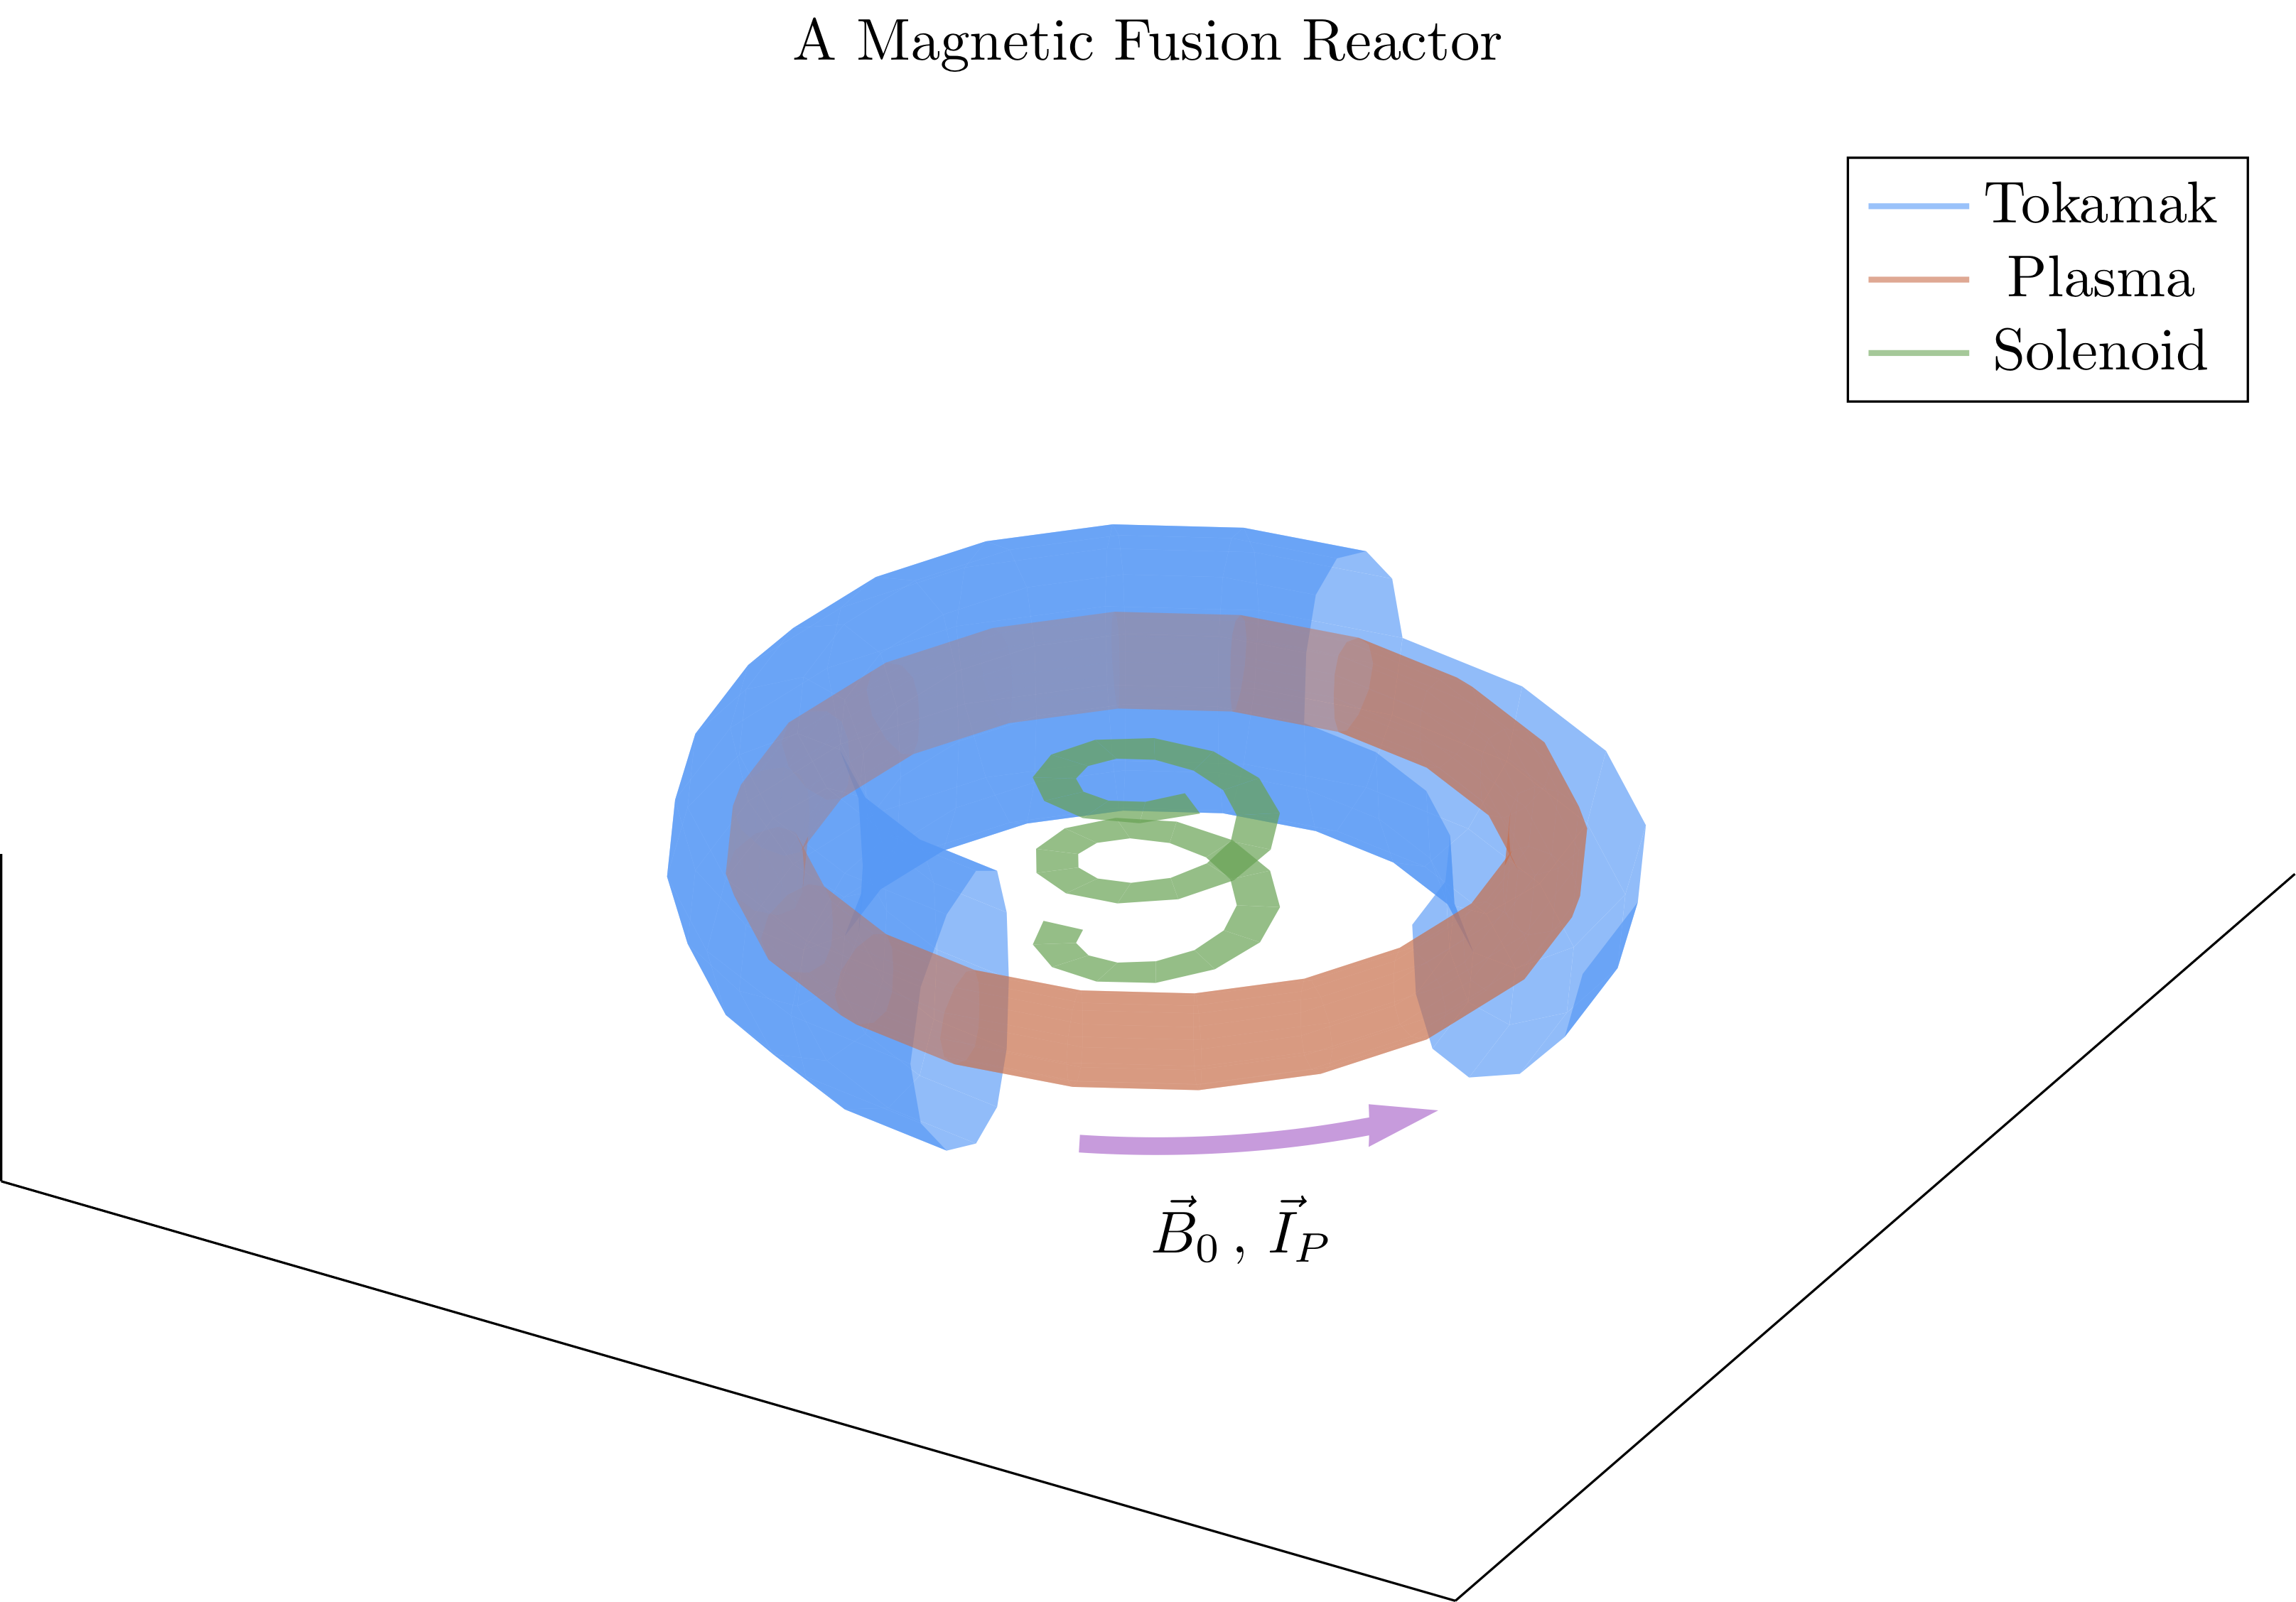
\includegraphics[width=0.75\textwidth]{images/fusion_reactor}
	\caption{Cut-Away of Tokamak Reactor} ~\\
	\small The three main components of a magnetic fusion reactor are: the tokamak structure, the plasma fuel, and the spring-like solenoid at the center. Here, the directions of the magnetic field ($B_0$) and plasma current ($I_P$) variables are shown to be in the toroidal direction.
	\label{fig:fusion_reactor}
\end{figure}

\added{The central goal of fusion energy research is to build an economically competitive nuclear reactor. It has long been joked, though, that fusion power will always be twenty years away. This is mainly due to the nonlinearities inherent to a reactor system and the high upfront cost of building new machines. The model developed for this paper uses standard theory and empirical fits to find cost trends from this nonlinear system. An important conclusion is that building an economic reactor using existing technology would be impossible. One solution may be improving magnet technology -- as MIT is exploring with high-temperature superconducting (HTS) tape.}

\added{As can be seen by comparing the European and American/Asian fusion reactor design efforts, though, one of the most important decisions is whether to run the reactor as pulsed (EU\cite{eupulsed,eupulsed_2}) or steady-state (US\cite{ussteady} and Korea\cite{kstar}). The distinction between the two mainly manifests itself in the choice of auxiliary current drive:  inductive  for pulsed and lower hybrid for steady-state.\cite{jeff} With the model built for this thesis, it is possible to perform a direct comparison of these two modes of operations. }

\added{Due to the speed and simplicity of the model, hundreds of reactors can be simulated in minutes. Further, the model has been benchmarked against other ones from the literature\cite{ussteady,arc,process,inputfile}, allowing it to answer several critical questions regarding the comparison of the two modes of operation. A major finding of this is that HTS tape should appear in different places for the two modes of operation: within the central solenoid for pulsed machines and inside the TF coil magnets for steady-state ones. A more basic finding is that pulsed can be competitive and the US should investigate it further. }

\deleted{The central goal of fusion energy research is to build a profitable nuclear reactor. It has long been joked though that fusion power will always be 20-50 years away. This paper lays a framework for exploring reactor space for functional, efficient designs -- based on world experiments during the last half-century. Due to the speed and simplicity of the model, hundreds of reactors can be explored in minutes (outpacing the domestic program slightly).}

\deleted{With this proposed model, interesting reactors can be pinpointed long before engineers hit the blueprints. This should help shorten the time until a profitable reactor, as well as illuminate ways to improve modern plasma theory. Further, it verifies the reasoning of MIT's PSFC to invest in high field, high-temperature superconducting (HTS) tape -- as this technology would lead to much smaller devices.}

\section{Distinguishing Pulsed from Steady-State}

\added{The leading candidate for the first economic, power-producing fusion reactor is a tokamak. As shown in \cref{fig:fusion_reactor}, tokamaks are doughnut-shaped metal structures that use magnets to confine their fusion-grade plasmas. The challenge in building such a device comes from the various physics and engineering constraints it must satisfy -- i.e. not surpassing acceptable levels of neutron damage, plasma pressure, etc.}

\added{One of the most contentious points of reactor design, however, is whether to run it as: pulsed (the European effort\cite{eupulsed,eupulsed_2}) or steady-state (the American/Asian approach\cite{ussteady,kstar}). Here, pulsed operation refers to how a reactor is ramped up and down several times a day. Whereas steady-state implies a machine is functionally kept ramped up the entirety of its fifty-year campaign. These behaviors are shown in \cref{fig:pulses}. The difficulties involves with the two modes of operation are then: cyclical stresses for pulsed and expensive current drive for steady state.\cite{jeff}}

\deleted{When people talk about fusion, they usually talk about plasma physics, and when people talk about plasma physics, they often talk about things like: the sun, lightning, and the aurora borealis. Of these three, the sun is the only nuclear reactor. However, the sun can stay on all day because the massive gravity of its fuel source helps keep it self-contained in space. On Earth, this is not possible -- the plasma fuel needs to be contained by other means (i.e.\ with magnets).}

%\footnote{Plasmas are the fourth state of matter after: solids, liquids, and gases. Fundamentally they are gaseous fluids that respond to electric and magnetic fields.}

\deleted{A tokamak is one of the leading candidates for a profitable fusion reactor. It shares the shape of a doughnut, using magnets to keep a hula hoop of plasma swirling inside it. The difficulty of keeping this plasma swirling though, is that it does not enjoy being spun too fast or squeezed too hard. Conversely, the tokamak housing the plasma does not like taking too much of a beating or being scaled to T-Rex sized proportions. This sets the stage for tokamak reactor design -- building on the various plasma physics and nuclear engineering constraints of the day. }

\deleted{One of the most contentious points of building a tokamak, however, is whether it will be run as: pulsed (the European approach \cite{eupulsed}) or steady-state (the United States effort \cite{ussteady}). Here, pulsed operation refers to how a reactor is turned on and off periodically -- around ten times a day. Whereas, steady state machines are meant to be left on nearly the entirety of their 50-year campaigns. These behaviors are shown in Fig.\ \ref{fig:pulses}.}

\begin{figure}
	\centering
	\begin{adjustbox}{width=0.65\textwidth}
		\large
		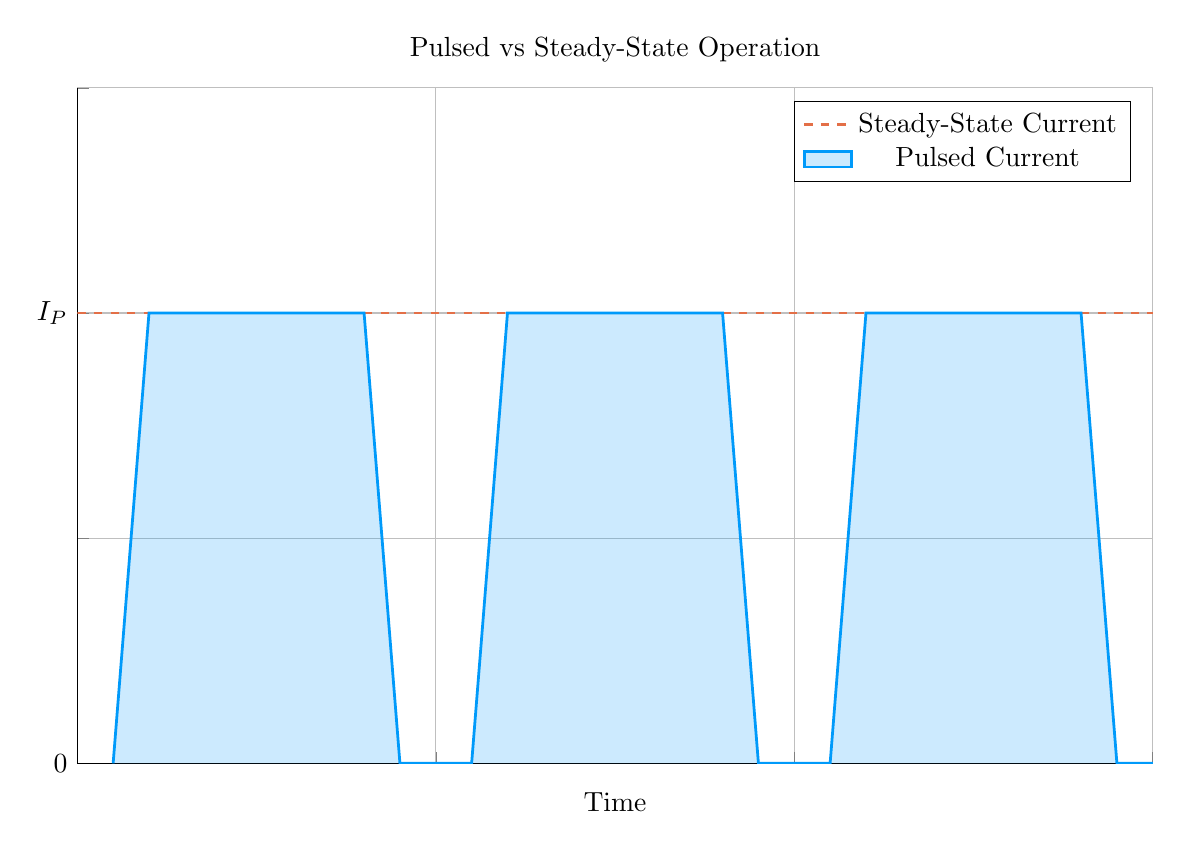
\begin{tikzpicture}[]
\begin{axis}[height = {101.6mm}, ylabel = {}, title = {Pulsed vs Steady-State Operation}, xmin = {0}, xmax = {30}, ymax = {1.5}, xlabel = {Time}, {unbounded coords=jump, scaled x ticks = false, xticklabel style={rotate = 0}, xmajorgrids = true, xtick = {10,20,30}, xticklabels = {}, xtick align = inside, axis lines* = left, scaled y ticks = false, yticklabel style={rotate = 0}, ymajorgrids = true, ytick = {0.0,0.5,1.0,1.5}, yticklabels = {0,,$I_P$,}, ytick align = inside, axis lines* = left,     xshift = 0.0mm,
    yshift = 0.0mm,
    axis background/.style={fill={rgb,1:red,1.00000000;green,1.00000000;blue,1.00000000}}
}, ymin = {0}, width = {152.4mm}]\addplot+ [color = {rgb,1:red,0.88887350;green,0.43564919;blue,0.27812294},
draw opacity=1.0,
line width=1,
dashed,mark = none,
mark size = 2.0,
mark options = {
    color = {rgb,1:red,0.00000000;green,0.00000000;blue,0.00000000}, draw opacity = 1.0,
    fill = {rgb,1:red,0.88887350;green,0.43564919;blue,0.27812294}, fill opacity = 1.0,
    line width = 1,
    rotate = 0,
    solid
}]coordinates {
(0.0, 1.0)
(2.0, 1.0)
(NaN, NaN)
(8.0, 1.0)
(12.0, 1.0)
(NaN, NaN)
(18.0, 1.0)
(22.0, 1.0)
(NaN, NaN)
(28.0, 1.0)
(30.0, 1.0)
};
\addlegendentry{Steady-State Current}
\addplot+ [color = {rgb,1:red,0.00000000;green,0.60560316;blue,0.97868012},
draw opacity=1.0,
line width=1,
solid,mark = none,
mark size = 2.0,
mark options = {
    color = {rgb,1:red,0.00000000;green,0.00000000;blue,0.00000000}, draw opacity = 1.0,
    fill = {rgb,1:red,0.00000000;green,0.60560316;blue,0.97868012}, fill opacity = 1.0,
    line width = 1,
    rotate = 0,
    solid
},fill = {rgb,1:red,0.00000000;green,0.60560316;blue,0.97868012}, fill opacity=0.2,area legend]coordinates {
(1, 0)
(2, 1)
(8, 1)
(9, 0)
(11, 0)
(11, 0)
(12, 1)
(18, 1)
(19, 0)
(21, 0)
(21, 0)
(22, 1)
(28, 1)
(29, 0)
(31, 0)
};
\addlegendentry{Pulsed Current}
\end{axis}

\end{tikzpicture}

	\end{adjustbox}
%	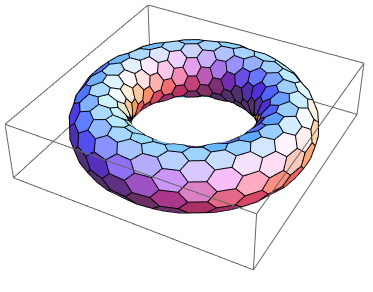
\includegraphics[width=0.85\textwidth]{images/test_image}
	\caption{Comparison of Pulsed and Steady-State Current} ~\\
	\small Inside a pulsed reactor, current is ramped up and down several times a day -- with downtime in-between. Steady state reactors are meant to remain on for weeks or months.
	\label{fig:pulses}
\end{figure}

\replaced{The main way these}{These} two modes of operation, \emph{pulsed} and \emph{steady-state}, \deleted{greatly} influence \replaced{reactor design, though, is}{the design} through the current balance equation (derived later). What this means practically is \replaced{a tokamak plasma requires some current to stay in equilibrium}{tokamaks need current to spin their plasma hoops at some required speed} and this current has to \replaced{be partially generated by auxiliary systems: inductively for pulsed and non-inductively for steady-state.}{come from somewhere. Luckily, the plasma naturally enjoys spinning and provides some assistance through the bootstrap current. The remaining current must then be produced by external means.} \added{To fairly compare the two modes of operation thus requires a generalized handling of current balance that can incorporate both auxiliary systems. }

\deleted{The source of external current drive is what distinguishes pulsed from steady-state devices. Steady-state devices provide the required current assistance either through lasers or particle beams -- this paper's model focusing on a type of laser assistance called lower-hybrid current drive (LHCD). \cite{jeff} Pulsed machines, on the other hand, rely on inductive sources -- which by definition require cycles of charging and discharging several times a day.}

%\footnote{ These inductive sources are akin to a battery on a laptop that must be recharged every so often. }

\deleted{The goal of this document is to show that pulsed and steady-state operation are actually two sides of the same coin. This yields the simple conclusion that a single comprehensive model can run both modes at the flip of a switch. It even opens the opportunity of a hybrid reactor that exists somewhere in between the two.}

%\section{Treating Fusion as a Business}
%
%Plasmas may be interesting, but that is not why countries build billion dollar research experiments. The ultimate goal of fusion research is to develop an energy resource that competes with coal and other base-load power sources (e.g.\ from hydroelectric and nuclear fission power plants). The problem is plasmas are chaotic and hard to contain, while tokamaks are expensive and slow to build. This perfect match has long put the field's projected timeline to that of \emph{fusion never}. \cite{fusionfunding}
%
%\begin{figure}[h]
%	\centering
%	\begin{adjustbox}{width=0.75\textwidth}
%		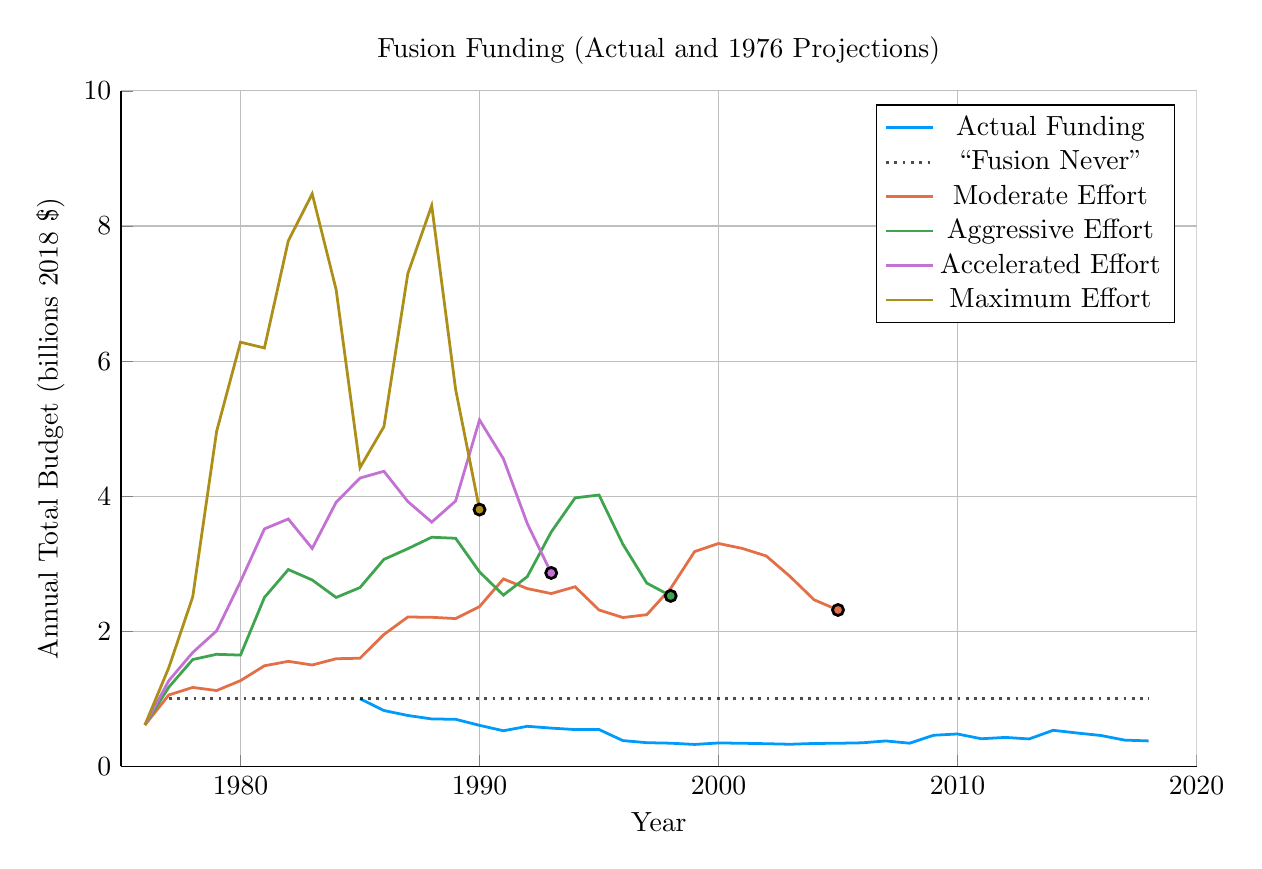
\begin{tikzpicture}[]
\begin{axis}[height = {101.6mm}, ylabel = {Annual Total Budget (billions 2018 \$)}, title = {Fusion Funding (Actual and 1976 Projections)}, xmin = {1975}, xmax = {2020}, ymax = {10}, xlabel = {Year}, {unbounded coords=jump, scaled x ticks = false, xticklabel style={rotate = 0}, xmajorgrids = true, xtick = {1980.0,1990.0,2000.0,2010.0,2020.0}, xticklabels = {1980,1990,2000,2010,2020}, xtick align = inside, axis lines* = left, scaled y ticks = false, yticklabel style={rotate = 0}, ymajorgrids = true, ytick = {0.0,2.0,4.0,6.0,8.0,10.0}, yticklabels = {0,2,4,6,8,10}, ytick align = inside, axis lines* = left,     xshift = 0.0mm,
    yshift = 0.0mm,
    axis background/.style={fill={rgb,1:red,1.00000000;green,1.00000000;blue,1.00000000}}
}, ymin = {0}, width = {152.4mm}]\addplot+ [color = {rgb,1:red,0.00000000;green,0.60560316;blue,0.97868012},
draw opacity=1.0,
line width=1,
solid,mark = none,
mark size = 2.0,
mark options = {
    color = {rgb,1:red,0.00000000;green,0.00000000;blue,0.00000000}, draw opacity = 1.0,
    fill = {rgb,1:red,0.00000000;green,0.60560316;blue,0.97868012}, fill opacity = 1.0,
    line width = 1,
    rotate = 0,
    solid
}]coordinates {
(1985.0, 1.001836)
(1986.0, 0.827367)
(1987.0, 0.754179)
(1988.0, 0.702929)
(1989.0, 0.697497)
(1990.0, 0.608102)
(1991.0, 0.527899)
(1992.0, 0.593976)
(1993.0, 0.567297)
(1994.0, 0.545463)
(1995.0, 0.545963)
(1996.0, 0.382175)
(1997.0, 0.351267)
(1998.0, 0.343818)
(1999.0, 0.325482)
(2000.0, 0.347117)
(2001.0, 0.342814)
(2002.0, 0.336267)
(2003.0, 0.32825)
(2004.0, 0.339832)
(2005.0, 0.342925)
(2006.0, 0.349302)
(2007.0, 0.377075)
(2008.0, 0.343662)
(2009.0, 0.461341)
(2010.0, 0.48051)
(2011.0, 0.409602)
(2012.0, 0.42938)
(2013.0, 0.406833)
(2014.0, 0.534818)
(2015.0, 0.494834)
(2016.0, 0.457833)
(2017.0, 0.389125)
(2018.0, 0.377419)
};
\addlegendentry{Actual Funding}
\addplot+ [color = {rgb,1:red,0.00000000;green,0.00000000;blue,0.00000000},
draw opacity=0.7,
line width=1,
dotted,mark = none,
mark size = 2.0,
mark options = {
    color = {rgb,1:red,0.00000000;green,0.00000000;blue,0.00000000}, draw opacity = 0.7,
    fill = {rgb,1:red,0.00000000;green,0.00000000;blue,0.00000000}, fill opacity = 0.7,
    line width = 1,
    rotate = 0,
    solid
}]coordinates {
(1977, 1)
(2018, 1)
};
\addlegendentry{``Fusion Never''}
\addplot+ [color = {rgb,1:red,0.88887350;green,0.43564919;blue,0.27812294},
draw opacity=1.0,
line width=1,
solid,mark = none,
mark size = 2.0,
mark options = {
    color = {rgb,1:red,0.00000000;green,0.00000000;blue,0.00000000}, draw opacity = 1.0,
    fill = {rgb,1:red,0.88887350;green,0.43564919;blue,0.27812294}, fill opacity = 1.0,
    line width = 1,
    rotate = 0,
    solid
}]coordinates {
(1976.0, 0.61374)
(1977.0, 1.05764)
(1978.0, 1.1695799999999998)
(1979.0, 1.12326)
(1980.0, 1.2699399999999998)
(1981.0, 1.48996)
(1982.0, 1.55558)
(1983.0, 1.5015399999999999)
(1984.0, 1.59418)
(1985.0, 1.6018999999999999)
(1986.0, 1.9531599999999998)
(1987.0, 2.2117799999999996)
(1988.0, 2.2079199999999997)
(1989.0, 2.18862)
(1990.0, 2.36618)
(1991.0, 2.77534)
(1992.0, 2.63252)
(1993.0, 2.55918)
(1994.0, 2.65954)
(1995.0, 2.316)
(1996.0, 2.2040599999999997)
(1997.0, 2.24652)
(1998.0, 2.63638)
(1999.0, 3.18064)
(2000.0, 3.3002999999999996)
(2001.0, 3.2269599999999996)
(2002.0, 3.11502)
(2003.0, 2.8100799999999997)
(2004.0, 2.4665399999999997)
(2005.0, 2.316)
};
\addlegendentry{Moderate Effort}
\addplot+[draw=none, color = {rgb,1:red,0.88887350;green,0.43564919;blue,0.27812294},
draw opacity=1.0,
line width=0,
solid,mark = *,
mark size = 2.0,
mark options = {
    color = {rgb,1:red,0.00000000;green,0.00000000;blue,0.00000000}, draw opacity = 1.0,
    fill = {rgb,1:red,0.88887350;green,0.43564919;blue,0.27812294}, fill opacity = 1.0,
    line width = 1,
    rotate = 0,
    solid
},forget plot] coordinates {
(2005.0, 2.316)
};
\addplot+ [color = {rgb,1:red,0.24222430;green,0.64327509;blue,0.30444865},
draw opacity=1.0,
line width=1,
solid,mark = none,
mark size = 2.0,
mark options = {
    color = {rgb,1:red,0.00000000;green,0.00000000;blue,0.00000000}, draw opacity = 1.0,
    fill = {rgb,1:red,0.24222430;green,0.64327509;blue,0.30444865}, fill opacity = 1.0,
    line width = 1,
    rotate = 0,
    solid
}]coordinates {
(1976.0, 0.61374)
(1977.0, 1.1734399999999998)
(1978.0, 1.5825999999999998)
(1979.0, 1.6598)
(1980.0, 1.6482199999999998)
(1981.0, 2.50128)
(1982.0, 2.9143)
(1983.0, 2.7598999999999996)
(1984.0, 2.50128)
(1985.0, 2.64796)
(1986.0, 3.06484)
(1987.0, 3.2230999999999996)
(1988.0, 3.39294)
(1989.0, 3.3775)
(1990.0, 2.8795599999999997)
(1991.0, 2.5360199999999997)
(1992.0, 2.8100799999999997)
(1993.0, 3.47014)
(1994.0, 3.9757999999999996)
(1995.0, 4.01826)
(1996.0, 3.2887199999999996)
(1997.0, 2.71358)
(1998.0, 2.52444)
};
\addlegendentry{Aggressive Effort}
\addplot+[draw=none, color = {rgb,1:red,0.24222430;green,0.64327509;blue,0.30444865},
draw opacity=1.0,
line width=0,
solid,mark = *,
mark size = 2.0,
mark options = {
    color = {rgb,1:red,0.00000000;green,0.00000000;blue,0.00000000}, draw opacity = 1.0,
    fill = {rgb,1:red,0.24222430;green,0.64327509;blue,0.30444865}, fill opacity = 1.0,
    line width = 1,
    rotate = 0,
    solid
},forget plot] coordinates {
(1998.0, 2.52444)
};
\addplot+ [color = {rgb,1:red,0.76444018;green,0.44411178;blue,0.82429754},
draw opacity=1.0,
line width=1,
solid,mark = none,
mark size = 2.0,
mark options = {
    color = {rgb,1:red,0.00000000;green,0.00000000;blue,0.00000000}, draw opacity = 1.0,
    fill = {rgb,1:red,0.76444018;green,0.44411178;blue,0.82429754}, fill opacity = 1.0,
    line width = 1,
    rotate = 0,
    solid
}]coordinates {
(1976.0, 0.61374)
(1977.0, 1.2699399999999998)
(1978.0, 1.68682)
(1979.0, 2.0071999999999997)
(1980.0, 2.7367399999999997)
(1981.0, 3.51646)
(1982.0, 3.66314)
(1983.0, 3.2269599999999996)
(1984.0, 3.9101799999999995)
(1985.0, 4.269159999999999)
(1986.0, 4.36952)
(1987.0, 3.92176)
(1988.0, 3.6168199999999997)
(1989.0, 3.92948)
(1990.0, 5.1299399999999995)
(1991.0, 4.554799999999999)
(1992.0, 3.59366)
(1993.0, 2.8641199999999998)
};
\addlegendentry{Accelerated Effort}
\addplot+[draw=none, color = {rgb,1:red,0.76444018;green,0.44411178;blue,0.82429754},
draw opacity=1.0,
line width=0,
solid,mark = *,
mark size = 2.0,
mark options = {
    color = {rgb,1:red,0.00000000;green,0.00000000;blue,0.00000000}, draw opacity = 1.0,
    fill = {rgb,1:red,0.76444018;green,0.44411178;blue,0.82429754}, fill opacity = 1.0,
    line width = 1,
    rotate = 0,
    solid
},forget plot] coordinates {
(1993.0, 2.8641199999999998)
};
\addplot+ [color = {rgb,1:red,0.67554396;green,0.55566233;blue,0.09423434},
draw opacity=1.0,
line width=1,
solid,mark = none,
mark size = 2.0,
mark options = {
    color = {rgb,1:red,0.00000000;green,0.00000000;blue,0.00000000}, draw opacity = 1.0,
    fill = {rgb,1:red,0.67554396;green,0.55566233;blue,0.09423434}, fill opacity = 1.0,
    line width = 1,
    rotate = 0,
    solid
}]coordinates {
(1976.0, 0.61374)
(1977.0, 1.46294)
(1978.0, 2.509)
(1979.0, 4.9601)
(1980.0, 6.28022)
(1981.0, 6.1953)
(1982.0, 7.781759999999999)
(1983.0, 8.47656)
(1984.0, 7.059939999999999)
(1985.0, 4.423559999999999)
(1986.0, 5.029579999999999)
(1987.0, 7.2954)
(1988.0, 8.302859999999999)
(1989.0, 5.58156)
(1990.0, 3.8021)
};
\addlegendentry{Maximum Effort}
\addplot+[draw=none, color = {rgb,1:red,0.67554396;green,0.55566233;blue,0.09423434},
draw opacity=1.0,
line width=0,
solid,mark = *,
mark size = 2.0,
mark options = {
    color = {rgb,1:red,0.00000000;green,0.00000000;blue,0.00000000}, draw opacity = 1.0,
    fill = {rgb,1:red,0.67554396;green,0.55566233;blue,0.09423434}, fill opacity = 1.0,
    line width = 1,
    rotate = 0,
    solid
},forget plot] coordinates {
(1990.0, 3.8021)
};
\end{axis}

\end{tikzpicture}

%	\end{adjustbox}
%%	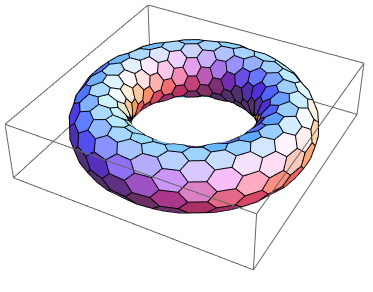
\includegraphics[width=0.75\textwidth]{images/test_image}
%	\caption{Fusion Never Funding Timeline} ~\\
%	\small Comparison of Projected Timelines of Fusion from 1976 with Actual DOE Budgets. \cite{doe87, doe19} \\ The dotted line is popularly referred to in the community as ``Fusion Never.'' \cite{fusionnever}
%\end{figure}
%
%The major problem with containing a plasma in a reactor is that a plasma does not want to be contained. Since the early days of fusion research, plasmas have often found escape mechanisms. When presented with a magnetic bottle, they found their way out the top. In a tokamak, they attack the outer edges like an overinflated tire-tube. Fusion energy has seemed to remain a Tantalizing effort -- within arms reach, but staunchly guarded by a shroud of instabilities.
%
%The truth is plasmas are extremely chaotic: they show nonlinear behavior in almost everything they do. As of now, no theory or supercomputer-backed code can predict even something so fundamental to design as the movement of energy and particles within a tokamak. As such, the field has adopted several rules of thumb and empirical scalings -- based on the last half century of experiments -- which help one navigate around a plasma's finicky behavior.
%
%The two most widely used rules of thumb within the fusion design community are: the Greenwald density limit and the ELMy H-Mode confinement time scaling law. As such, the model in this document heavily utilizes the two to make a quick running code. These two relations are also why this model -- which happens to be zero-dimensional -- can reproduce with high fidelity the answers from three-dimensional codes, which can take days, weeks, or even months to run!
%
%\begin{figure}
%	\centering
%	\begin{adjustbox}{width=0.75\textwidth}
%		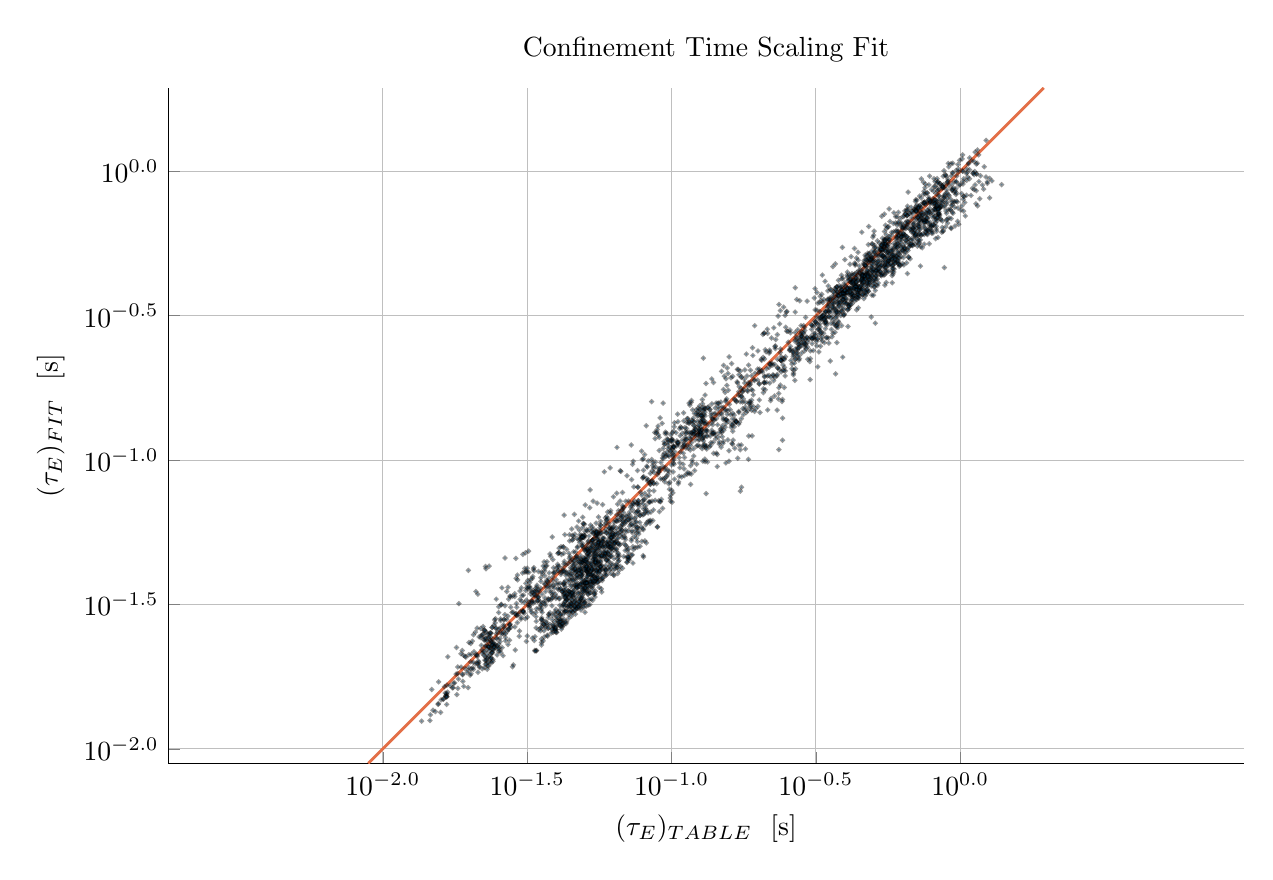
\begin{tikzpicture}[]
\begin{axis}[height = {101.6mm}, axis equal = {true}, ylabel = {$(\tau_E)_{ FIT } \ \ [ \textnormal{s} ]$}, title = {Confinement Time Scaling Fit}, xmin = {0.008904842990761705}, xmax = {1.9473999999999996}, ymax = {1.9473999999999996}, ymode = {log}, xlabel = {$(\tau_E)_{ TABLE } \ \ [ \textnormal{s} ]$}, {unbounded coords=jump, scaled x ticks = false, xticklabel style={rotate = 0}, log basis x=10, xmajorgrids = true, xtick = {0.01,0.03162277660168379,0.1,0.31622776601683794,1.0}, xticklabels = {$10^{-2.0}$,$10^{-1.5}$,$10^{-1.0}$,$10^{-0.5}$,$10^{0.0}$}, xtick align = inside, axis lines* = left, scaled y ticks = false, yticklabel style={rotate = 0}, log basis y=10, ymajorgrids = true, ytick = {0.01,0.03162277660168379,0.1,0.31622776601683794,1.0}, yticklabels = {$10^{-2.0}$,$10^{-1.5}$,$10^{-1.0}$,$10^{-0.5}$,$10^{0.0}$}, ytick align = inside, axis lines* = left,     xshift = 0.0mm,
    yshift = 0.0mm,
    axis background/.style={fill={rgb,1:red,1.00000000;green,1.00000000;blue,1.00000000}}
}, xmode = {log}, ymin = {0.008904842990761705}, width = {152.4mm}]\addplot+[draw=none, color = {rgb,1:red,0.00000000;green,0.60560316;blue,0.97868012},
draw opacity=0.4,
line width=0,
solid,mark = *,
mark size = 0.325,
mark options = {
    color = {rgb,1:red,0.00000000;green,0.00000000;blue,0.00000000}, draw opacity = 0.4,
    fill = {rgb,1:red,0.00000000;green,0.60560316;blue,0.97868012}, fill opacity = 0.4,
    line width = 1,
    rotate = 0,
    solid
},forget plot] coordinates {
(0.048709999999999996, 0.03286927009465151)
(0.047479999999999994, 0.030718782340371346)
(0.056709999999999997, 0.04427687673230967)
(0.06154, 0.040523205193333994)
(0.049249999999999995, 0.031000215657666388)
(0.046439999999999995, 0.03902384637413358)
(0.04536, 0.03366158264691253)
(0.041229999999999996, 0.029311430641277475)
(0.04224, 0.03489492877112558)
(0.05357, 0.03985677848149215)
(0.042449999999999995, 0.030139467297048302)
(0.04393, 0.03525642598465171)
(0.037579999999999995, 0.029115058174186102)
(0.040589999999999994, 0.03552938448965956)
(0.016339999999999997, 0.016414220556232706)
(0.01926, 0.018966660638066977)
(0.014769999999999998, 0.01604916788911629)
(0.020909999999999998, 0.019687625330862386)
(0.014559999999999998, 0.01252323235667468)
(0.016659999999999998, 0.016615842361327)
(0.017099999999999997, 0.016562775820865377)
(0.025429999999999998, 0.024119656293897448)
(0.01834, 0.03183654298531315)
(0.02225, 0.026522518089311862)
(0.02354, 0.023762954142859543)
(0.01883, 0.02190554572449257)
(0.0156, 0.0170549295762654)
(0.01678, 0.020822704009415233)
(0.154, 0.14943255990407037)
(0.17639999999999997, 0.1506224447310805)
(0.7525999999999999, 0.7841653529419872)
(0.7196999999999999, 0.7123510444198007)
(0.7581, 0.7126653992395249)
(0.5971, 0.6636747785042374)
(0.5545, 0.6034081737695671)
(0.5620999999999999, 0.5855426425362842)
(0.7231, 0.611757051674103)
(0.7314999999999999, 0.6000776436052295)
(0.8261999999999999, 0.7332080576221435)
(0.8526999999999999, 0.6874473851854792)
(0.7659999999999999, 0.6249854199535853)
(0.8212999999999999, 0.6647675128338589)
(0.7968, 0.6202645990011652)
(1.1369999999999998, 0.8572954951071405)
(0.8379, 0.709498458538988)
(0.7112999999999999, 0.6481476339591892)
(0.8383999999999999, 0.7100253242029977)
(0.9772, 0.7850517774047457)
(0.6932999999999999, 0.6449986085844157)
(0.7078, 0.5696128161569505)
(0.7666999999999999, 0.6076651618162499)
(0.7231, 0.8218656209469912)
(0.7654, 0.7824204839027497)
(0.8880999999999999, 0.9751544259782554)
(0.9436, 0.987045215482296)
(0.982, 1.0567556111003251)
(1.0659999999999998, 1.0600221351309262)
(1.021, 1.0023421135083617)
(1.037, 0.780421246365204)
(1.0139999999999998, 0.7598649860996711)
(0.9391999999999999, 0.722374477345195)
(0.7876, 0.7737488110528499)
(0.7564, 0.8355652777917266)
(0.8073999999999999, 0.7829615268340135)
(0.6101, 0.662119064106307)
(0.5015, 0.6015695673902948)
(0.7323999999999999, 0.8090796506003152)
(0.6535, 0.7394639493973881)
(0.5972, 0.6975536633839833)
(0.8778999999999999, 0.7874999827504517)
(0.7773, 0.8125562886500788)
(0.6810999999999999, 0.7238692523345119)
(0.6392, 0.701072652615907)
(0.6046999999999999, 0.6507248504722397)
(0.9085, 1.0662323587837632)
(0.746, 0.9171741777262944)
(0.6601999999999999, 0.8477587902173862)
(1.019, 1.1402820961295275)
(0.9123, 1.0371038527895822)
(0.5081, 0.5255375119481419)
(0.7402, 0.6843189302449205)
(0.7313999999999999, 0.6912025500896107)
(1.0779999999999998, 1.1138270195034614)
(0.6314, 0.6309700937894861)
(0.9303999999999999, 0.9647835607071941)
(0.8503, 0.9084098651600415)
(0.8125, 0.8871934724039697)
(0.9943, 1.0920838325900788)
(0.8109999999999999, 0.94316240550339)
(0.7583, 0.9027068941508603)
(0.8357, 0.9197400869136341)
(0.6762999999999999, 0.7509390530838264)
(0.6529999999999999, 0.7031904860947172)
(0.3892, 0.34318485870648646)
(0.34049999999999997, 0.3124029593731834)
(0.45299999999999996, 0.3908324185235881)
(0.44149999999999995, 0.37445805641759866)
(0.5680999999999999, 0.519309036063986)
(0.5427, 0.470258508275619)
(0.3973, 0.3208880474419727)
(0.4023, 0.3620545624474692)
(0.36279999999999996, 0.3723269788644909)
(0.5475, 0.4394327211967968)
(0.3898, 0.37922457801357046)
(0.31279999999999997, 0.303118325347936)
(0.38389999999999996, 0.35281373501460195)
(0.3181, 0.31386085182034285)
(0.7142, 0.6930925801653104)
(0.6252, 0.6626568011479417)
(0.6154999999999999, 0.5263153459242683)
(0.9141999999999999, 0.6902582143865932)
(0.7587999999999999, 0.6215886466745869)
(0.6337999999999999, 0.5997015869390643)
(0.9221999999999999, 0.7382203149764545)
(0.6928, 0.6177290812059213)
(0.7125999999999999, 0.6963967594591091)
(0.21899999999999997, 0.18496435234301067)
(0.20789999999999997, 0.1766203805469118)
(0.26499999999999996, 0.20490261922028621)
(0.4225, 0.34891440428748743)
(0.4118, 0.3421446077261888)
(0.2397, 0.22159945467095882)
(0.26959999999999995, 0.22409261472703068)
(0.3127, 0.2631427459860977)
(0.32389999999999997, 0.2832737570128158)
(0.8515999999999999, 0.9068928303444452)
(0.8177, 0.9220516908419841)
(1.0179999999999998, 1.002889177259622)
(0.5892999999999999, 0.7186483132855688)
(0.9675999999999999, 0.918899482262656)
(0.8809999999999999, 0.4645188486258639)
(1.077, 1.013495270683344)
(0.5667, 0.7415870515780109)
(0.5344, 0.6992580529977903)
(0.5457, 0.7114200487063042)
(0.6599999999999999, 0.568829584256022)
(0.7506999999999999, 0.604323636235005)
(0.7131, 0.5987909231331726)
(0.6576, 0.5815966808550769)
(0.6386, 0.6040200009888924)
(0.4816, 0.6444934910993216)
(0.45589999999999997, 0.6160051006574458)
(0.6427999999999999, 0.7305600248168257)
(0.8285999999999999, 0.7476043736628556)
(0.6534, 0.6544069370264392)
(0.6638999999999999, 0.6723198321350972)
(0.5883999999999999, 0.5629685596654105)
(0.6073999999999999, 0.5947667114406178)
(0.5639, 0.5731530731910407)
(0.6101, 0.6034835968431853)
(0.6638999999999999, 0.5863468310710566)
(0.6346999999999999, 0.5309682418246683)
(0.5062, 0.456996379113654)
(0.6548999999999999, 0.703107054401337)
(0.5526, 0.5545528151553201)
(0.8658999999999999, 0.7858011508612296)
(0.7361, 0.7026740161837454)
(0.734, 0.7080907193345652)
(0.722, 0.7026124938878728)
(0.9287, 1.0629014859458583)
(0.7698999999999999, 0.84074579772222)
(0.8176, 0.8870105921186713)
(0.5843999999999999, 0.5035404234450113)
(0.9373999999999999, 0.8698220688660848)
(0.9337, 0.8623382177770421)
(0.8964, 0.7160170198322513)
(0.7332, 0.9423078640879671)
(0.7831999999999999, 0.963224279565402)
(0.9906999999999999, 0.8952623033567918)
(0.9087, 0.8308130537672082)
(0.7955, 0.8658102097350978)
(0.9360999999999999, 0.9039593399896794)
(0.7863, 0.714131359979918)
(0.8229, 0.740299033130453)
(0.823, 0.760314511413916)
(0.7636999999999999, 0.7163144408463683)
(0.6311, 0.5556779797096207)
(0.6262, 0.6533313908678976)
(0.8946999999999999, 0.9586908006605939)
(0.8576999999999999, 0.7537146014939096)
(0.8473999999999999, 0.7461424250229518)
(0.9255, 0.801575405231461)
(0.8498, 0.7649223531344689)
(0.7823, 0.7268518889656576)
(0.8255999999999999, 0.7470872412684922)
(0.8631, 0.7753860665056598)
(0.7994, 0.728145541191726)
(0.8747999999999999, 0.8208827079316118)
(1.015, 1.1045865073889138)
(1.1609999999999998, 0.9219761380746218)
(0.7623, 0.6715119057586799)
(0.7824, 0.6467686006890678)
(0.5243, 0.564617572937227)
(0.5503999999999999, 0.5783318044105018)
(0.5407, 0.5701439812605221)
(0.5317999999999999, 0.5494542896098417)
(0.5491999999999999, 0.5670933149802504)
(0.5455, 0.5598085924937554)
(0.8478, 0.7018507562099994)
(0.7223999999999999, 0.6570441876740942)
(0.8067, 0.7135500971429034)
(0.7686999999999999, 0.6885128255514706)
(0.7448999999999999, 0.6760240646258281)
(0.7343, 0.6742929760912958)
(0.6597999999999999, 0.7354882011318915)
(0.6793999999999999, 0.7289884081681665)
(0.6546, 0.7051597393592424)
(0.9087999999999999, 0.7368656746766299)
(0.7526999999999999, 0.671806203783079)
(0.7545, 0.8781283223894364)
(0.969, 1.0091726548574242)
(0.9864999999999999, 0.9978820947672817)
(0.9519, 0.8476711232851686)
(0.8273999999999999, 0.778663500363082)
(0.8248, 0.7801934517664398)
(0.6835, 0.6627837535553688)
(0.6928, 0.6114247462326845)
(0.7931999999999999, 0.6269714335560767)
(0.7208, 0.6045147201505461)
(0.6963999999999999, 0.6028585041743847)
(0.8253999999999999, 0.6317543998575686)
(0.6675, 0.5602136085491106)
(0.7319, 0.6026263780884397)
(0.6533, 0.5360321914526158)
(0.564, 0.4904554472531542)
(0.9439, 0.7157171194446946)
(0.7939999999999999, 0.6411620402371146)
(0.8091999999999999, 0.6525781912908896)
(0.7292, 0.5485933677696657)
(0.6357999999999999, 0.503286345980577)
(0.6447999999999999, 0.5185162967617107)
(1.069, 1.0695180372896376)
(0.8583, 0.8908809768320126)
(0.8087, 0.8543034142940075)
(0.8318, 0.9446369769051516)
(0.7786, 0.8979525071302351)
(1.1219999999999999, 0.9996281574893591)
(1.107, 0.9853860242113884)
(1.2109999999999999, 1.0380777356700828)
(1.109, 0.988185626984255)
(0.8967999999999999, 0.7722301840545289)
(0.824, 0.8390911317907782)
(0.8246, 0.7494173273698013)
(0.7246999999999999, 0.6803976433290927)
(0.6926, 0.6607682224597816)
(0.8103999999999999, 0.7710346210832281)
(0.7748999999999999, 0.7325112272388337)
(0.7414999999999999, 0.7062682017319861)
(0.8249, 0.6842066249663288)
(0.8475999999999999, 0.7093971409693103)
(0.7781999999999999, 0.6302194723063099)
(0.7003999999999999, 0.6008831528899192)
(0.6518999999999999, 0.5945976708252837)
(0.7195999999999999, 0.5780911978357602)
(0.7698999999999999, 0.6045774400058568)
(0.6951999999999999, 0.5594902956731888)
(0.6265999999999999, 0.5281946682083224)
(1.0519999999999998, 0.9316449640552941)
(1.011, 0.8373271253227542)
(1.0619999999999998, 0.9564802790915702)
(0.9991, 0.8998058834673238)
(1.1019999999999999, 0.874362127898913)
(0.9502999999999999, 0.7861813492490419)
(1.1929999999999998, 0.8970574608241824)
(1.1409999999999998, 0.9798783118539908)
(1.1389999999999998, 0.981247441890904)
(0.7454, 0.6506062999832742)
(0.7213999999999999, 0.6316980480914915)
(0.7511, 0.6382470829505086)
(1.168, 0.8045488413734408)
(1.1329999999999998, 0.7723998453123871)
(1.2049999999999998, 0.8686731269524)
(0.8418, 0.7105640304650586)
(0.8438, 0.7167529167481481)
(0.8319, 0.6761440014142099)
(0.7971999999999999, 0.647212185326572)
(0.8099999999999999, 0.6507837939912798)
(0.954, 0.7838744415871535)
(1.0279999999999998, 0.8191939822720388)
(1.029, 0.8188141254422304)
(0.9371999999999999, 0.765214397024378)
(1.0219999999999998, 0.9050020965486358)
(1.1449999999999998, 1.0674931488210169)
(1.136, 1.0609598989430766)
(0.9721, 0.9642173576087313)
(0.8966, 0.8641697646781274)
(0.8880999999999999, 0.8373748291165626)
(0.8997999999999999, 0.8442042621804475)
(1.0219999999999998, 0.9220333467704045)
(1.126, 0.897657994702853)
(1.2879999999999998, 0.9272527550966493)
(0.8389, 0.7182547844853155)
(0.9348, 0.7828004050235056)
(1.051, 0.8269739428545848)
(1.0239999999999998, 0.8005745674982954)
(1.158, 1.1412196875478482)
(0.8996, 0.8065770952173787)
(0.9666999999999999, 0.8315473131899693)
(0.8414999999999999, 0.7684067296642498)
(0.8493999999999999, 0.7527319188772996)
(0.8481, 0.7458196646149527)
(0.8429, 0.7423208728716764)
(0.8990999999999999, 0.7842614607464142)
(0.8253999999999999, 0.7485587864344085)
(0.8107, 0.7384132406448961)
(0.8147, 0.7410312659641048)
(0.9854999999999999, 1.0196276084818066)
(1.1469999999999998, 1.1863286392932)
(1.126, 1.1666665208852889)
(0.9404999999999999, 0.8611051902461748)
(0.7303, 0.7213915082892701)
(1.0959999999999999, 1.0877850615898468)
(1.117, 1.0833298051794935)
(1.057, 0.9923729605851154)
(0.9539, 0.9233369235535771)
(1.2289999999999999, 1.2805920757347342)
(0.8688999999999999, 0.8918437252115444)
(0.8352999999999999, 0.8716065387445937)
(0.9081999999999999, 0.9368678123602089)
(0.8755, 0.90002820580841)
(0.8695999999999999, 0.8794079728006472)
(0.8787999999999999, 0.881459737915593)
(0.9007, 0.9104206399267062)
(0.872, 0.8798842972291739)
(0.8658999999999999, 0.8749949687250976)
(0.8429, 0.8633412845042695)
(0.8341, 0.8574697533575164)
(0.7795, 0.80110995309816)
(0.8055, 0.8051314579770487)
(0.7888999999999999, 0.7871440794358052)
(0.7888, 0.78597297922507)
(0.7839999999999999, 0.783736968755363)
(0.8906999999999999, 0.9705362439027034)
(0.8353999999999999, 0.9206177853670467)
(0.9397, 0.9901636819697397)
(0.833, 0.9066645584090964)
(0.7091, 0.7411169895186779)
(0.7263999999999999, 0.7515058392068585)
(0.9071999999999999, 0.9226286568967264)
(0.8681, 0.8888136889786512)
(0.7014999999999999, 0.7549502980032216)
(0.6941999999999999, 0.7414453256597049)
(0.6193, 0.6868705118704591)
(0.7438999999999999, 0.7801456918201667)
(0.6958, 0.7373496835919023)
(0.7162, 0.7545932329675524)
(0.7295999999999999, 0.7653022211346575)
(0.7071, 0.7633267093779594)
(0.7009, 0.79841785676154)
(0.7074999999999999, 0.7960705831433198)
(0.6993999999999999, 0.7869623482126145)
(0.7202, 0.7611057495934285)
(0.7847999999999999, 0.7953466660425729)
(0.7509999999999999, 0.7704143379652046)
(0.6954999999999999, 0.7363969319361924)
(0.6666, 0.7152819454604417)
(0.7485999999999999, 0.7778447754623078)
(0.7101999999999999, 0.7347703554376556)
(0.6983999999999999, 0.7278364728917994)
(0.5580999999999999, 0.4833226862967873)
(0.6591999999999999, 0.5325006454360778)
(0.6224999999999999, 0.507999140907478)
(0.592, 0.4829571034104287)
(0.5678, 0.4750822637133591)
(0.5478999999999999, 0.46940311682153735)
(0.7485999999999999, 0.7775297709191064)
(0.7027, 0.7322537919167466)
(0.7165999999999999, 0.7453502012689315)
(0.7544, 0.7813252510105715)
(0.701, 0.7340106625957865)
(1.0499999999999998, 0.9847941321751483)
(0.7162, 0.7493085145738181)
(0.6687, 0.7135001121348747)
(0.7599999999999999, 0.768274815018355)
(0.7058, 0.7290656456829794)
(0.7031, 0.7275885380278503)
(0.7041, 0.6367181066561843)
(0.688, 0.6354802698552251)
(1.077, 0.943090689087118)
(0.9655999999999999, 0.8715157034912367)
(0.8762, 0.8088387283718785)
(0.8806999999999999, 0.8127564086172461)
(0.5542999999999999, 0.41253102576251693)
(0.5478, 0.4036039372001265)
(0.4941, 0.373031283060472)
(0.5829, 0.512947049410342)
(0.5613999999999999, 0.48664164380957775)
(0.5247999999999999, 0.4527986103525293)
(0.4695, 0.4227065708121077)
(0.48919999999999997, 0.5073610229958332)
(0.6664, 0.5504072752437238)
(0.6019, 0.506184963883185)
(0.5290999999999999, 0.46835384346341935)
(0.6813999999999999, 0.5595253856241379)
(0.5491999999999999, 0.47440537547191425)
(0.5149999999999999, 0.454161051345693)
(0.6145999999999999, 0.5153919313492221)
(0.5720999999999999, 0.48890197499449095)
(0.7011999999999999, 0.5951245600889739)
(0.6801999999999999, 0.5862584147630384)
(0.6436, 0.5779925943174439)
(0.6879, 0.6355711960485161)
(0.7161, 0.6580154715421902)
(0.6805, 0.6403947308683965)
(0.5677, 0.4994502254665087)
(0.6407999999999999, 0.537341813479382)
(0.5336, 0.4735622145714224)
(0.6022, 0.48585628016871496)
(0.5301999999999999, 0.43812776843405565)
(0.5569, 0.4511379734712108)
(0.5309999999999999, 0.4382828143980356)
(0.7189, 0.561283944496514)
(0.6033, 0.49593491486870384)
(0.5882, 0.48791409058918084)
(0.5133, 0.47086714482313546)
(0.6835, 0.5557071339364735)
(0.5457, 0.4595648149111282)
(0.5548, 0.46523133962452173)
(0.47969999999999996, 0.4249658620586939)
(0.4523, 0.415295964493189)
(0.6022, 0.5400209296818028)
(0.5538, 0.5052764641657136)
(0.5436, 0.5055194776119623)
(0.6782999999999999, 0.6163137196828592)
(0.695, 0.6266243673269388)
(0.62, 0.5813674172258797)
(0.6432, 0.5431537583550402)
(0.6287999999999999, 0.5349480622390502)
(0.6376, 0.54586058250559)
(0.5668, 0.4914002086290934)
(0.5511999999999999, 0.47842606650822395)
(0.5179999999999999, 0.4490979395028368)
(0.4926, 0.43740028298001615)
(0.45459999999999995, 0.4189036373559835)
(0.6536, 0.5941545657972782)
(0.5829, 0.5349527992919924)
(0.18815494499765392, 0.1581399078244611)
(0.2146061814556331, 0.19572896069781145)
(0.16599999999999998, 0.13799498658430565)
(0.18969999999999998, 0.14876546786696357)
(0.1833, 0.1482841294703696)
(0.1813, 0.14622039951602703)
(0.17729999999999999, 0.14361309282173648)
(0.1793, 0.14932396239540086)
(0.16018654635778376, 0.14375168149593862)
(0.23608148464163825, 0.20618864049175167)
(0.15090505517866634, 0.13993845766847318)
(0.16462308753545907, 0.14319802218703614)
(0.22867658825412063, 0.2432843316035902)
(0.15437048917401763, 0.19150835096181462)
(0.204407884525842, 0.2234568824525145)
(0.3385921358212541, 0.25515688094639516)
(0.30803062388011077, 0.2920590580475614)
(0.3698439872088892, 0.1989826760084809)
(0.3020055284361583, 0.1900834656284462)
(0.391747288185283, 0.22739364529660014)
(0.18722432262129804, 0.1513418397949884)
(0.35449272544635624, 0.220335621447283)
(0.23145587735894824, 0.1958237725659035)
(0.22568075547813332, 0.1966426493637936)
(0.12419999999999999, 0.12535236963339896)
(0.1362, 0.12116477109254274)
(0.1686, 0.18668565060566708)
(0.2571, 0.24065324034899624)
(0.14309999999999998, 0.10574864224466833)
(0.1001, 0.07861924902447287)
(0.1394, 0.11523665402006138)
(0.13169999999999998, 0.11054302384899538)
(0.1679, 0.16024914750084338)
(0.1679, 0.1592375423514523)
(0.1379, 0.1269124989160874)
(0.13759999999999997, 0.13474346567467413)
(0.15669999999999998, 0.11752104464678922)
(0.1634, 0.11731413030603775)
(0.1513, 0.11615944954854357)
(0.1641, 0.1342046675569159)
(0.1324, 0.11202070716494673)
(0.144, 0.10455225164776064)
(0.08367999999999999, 0.07550572887234856)
(0.08138, 0.06960465607403137)
(0.07985999999999999, 0.06790024415870552)
(0.06914, 0.06133434654420463)
(0.07455999999999999, 0.0659594636095902)
(0.06749, 0.059094960344554005)
(0.07956999999999999, 0.06457109181522346)
(0.07042, 0.06434532605690742)
(0.1243, 0.11740776302358609)
(0.1098, 0.10570841747417169)
(0.11209999999999999, 0.10998875997985506)
(0.12769999999999998, 0.10957807347983331)
(0.10719999999999999, 0.1065573371040371)
(0.13019999999999998, 0.11151703529901563)
(0.11929999999999999, 0.10336177621901224)
(0.18949999999999997, 0.16142608123554003)
(0.13319999999999999, 0.0985814769637825)
(0.122, 0.12133203045600598)
(0.13249999999999998, 0.12167416353208241)
(0.1772, 0.16311084283670516)
(0.11599999999999999, 0.12343156692499643)
(0.118, 0.12364896689819536)
(0.14439999999999997, 0.13258051012966407)
(0.08478999999999999, 0.06604715398119469)
(0.06265, 0.05571638354031536)
(0.06549999999999999, 0.05587664803721788)
(0.07185, 0.06281229971832496)
(0.09925999999999999, 0.07568059816491898)
(0.08231, 0.06687006216262115)
(0.10619999999999999, 0.08785115077712564)
(0.12229999999999999, 0.11192205816899478)
(0.11739999999999999, 0.11521568056327589)
(0.12789999999999999, 0.1567843318502842)
(0.13579999999999998, 0.14986674835019317)
(0.1419, 0.1450258373657531)
(0.16909999999999997, 0.18501546928802198)
(0.17149999999999999, 0.17951957710562474)
(0.1555, 0.1814374863085525)
(0.08192999999999999, 0.060625895818463005)
(0.054299999999999994, 0.04462659847247578)
(0.2382, 0.1819535561143575)
(0.09888999999999999, 0.07391663231244197)
(0.124, 0.14509661104394564)
(0.07007999999999999, 0.08833187686319875)
(0.1354, 0.11128291067705666)
(0.08912999999999999, 0.05866212753957971)
(0.09344, 0.10979611752819195)
(0.08574, 0.09185740084703009)
(0.07637999999999999, 0.08068943179070469)
(0.1404, 0.13841888959775664)
(0.09434999999999999, 0.10565360812919727)
(0.08445, 0.08995215787515654)
(0.07651, 0.08056048684717657)
(0.07107, 0.07211752477661636)
(0.06596999999999999, 0.06504025851381419)
(0.06323, 0.06094593014549412)
(0.12, 0.12630414943307358)
(0.1007, 0.10525729084649234)
(0.1108, 0.1020943378561658)
(0.1661, 0.16132082925344174)
(0.1372, 0.14528321511173972)
(0.15119999999999997, 0.1523332546589318)
(0.1488, 0.14590645549660508)
(0.1263, 0.13574445405586816)
(0.16479999999999997, 0.13044837625750083)
(0.1802, 0.15262991045375698)
(0.15419999999999998, 0.13767198793228275)
(0.2344, 0.16286922831246586)
(0.1619, 0.13198012828918207)
(0.1316, 0.1276676250276773)
(0.1719, 0.13525220987281406)
(0.1177, 0.09988977043209674)
(0.1011, 0.07701041806885227)
(0.1016, 0.09769656334934149)
(0.2014, 0.16156529514473916)
(0.12619999999999998, 0.1453260279389522)
(0.1273, 0.14152422005247894)
(0.10569999999999999, 0.11434661903762405)
(0.1306, 0.1680125891907873)
(0.1319, 0.13503314008427944)
(0.1026, 0.10687459020159086)
(0.09519999999999999, 0.09412923196453649)
(0.08876999999999999, 0.08283955952603496)
(0.10229999999999999, 0.08588833148769484)
(0.08658999999999999, 0.08299779138044373)
(0.12799999999999997, 0.14134838261978305)
(0.10079999999999999, 0.10946905609261658)
(0.09147999999999999, 0.09369943456869442)
(0.08574999999999999, 0.08482791867206357)
(0.08084, 0.0767519431544391)
(0.07662, 0.07222614911256207)
(0.1523, 0.19536945325599323)
(0.11299999999999999, 0.13487967435723913)
(0.10949999999999999, 0.11143501760664376)
(0.09051, 0.09340434624717418)
(0.08438999999999999, 0.08268489965566242)
(0.07891999999999999, 0.07556694845270819)
(0.07379999999999999, 0.07096169353245259)
(0.1397, 0.18575095007051093)
(0.13799999999999998, 0.14010775280450505)
(0.1104, 0.11206507718092389)
(0.102, 0.09676166903886248)
(0.09311, 0.08600781045736207)
(0.08688, 0.07826153594175268)
(0.08052999999999999, 0.07301355683925279)
(0.1487, 0.1442582464317744)
(0.1137, 0.11263854088300114)
(0.09999999999999999, 0.0962223851675817)
(0.09147999999999999, 0.08616202229912978)
(0.08366, 0.07830055417672487)
(0.07941999999999999, 0.0721875693170648)
(0.07307, 0.0675705560076057)
(0.143, 0.13914318897713676)
(0.23379999999999998, 0.31531076056144025)
(0.19399999999999998, 0.29205931398123475)
(0.149, 0.20306944284381495)
(0.09272999999999999, 0.13401719596726916)
(0.08355, 0.0716089079690666)
(0.09022, 0.07228247460420813)
(0.09165, 0.07174064320583198)
(0.11389999999999999, 0.13914314602381422)
(0.1133, 0.13923921674291376)
(0.11889999999999999, 0.1397352499217919)
(0.1568, 0.19945630712290494)
(0.156, 0.2085005358684465)
(0.1306, 0.09881166008611196)
(0.1283, 0.09913341046916643)
(0.08012999999999999, 0.07302668206755579)
(0.06458, 0.06144775295643559)
(0.08765999999999999, 0.07256126399136432)
(0.05644, 0.05559868896061745)
(0.06917999999999999, 0.06275059588936908)
(0.061579999999999996, 0.058396471040249004)
(0.07954, 0.07048587142644203)
(0.1114, 0.11994745431276213)
(0.1113, 0.11733327502135991)
(0.1148, 0.13484774445886444)
(0.11049999999999999, 0.11437476436659133)
(0.10729999999999999, 0.13021477026161207)
(0.1225, 0.13606696165153784)
(0.1157, 0.15513167323708593)
(0.11499999999999999, 0.13411837835876708)
(0.1306, 0.14213468350709502)
(0.08935, 0.08915179338374941)
(0.11009999999999999, 0.14576047007944345)
(0.1278, 0.1619777264626628)
(0.11689999999999999, 0.15853225680858268)
(0.1243, 0.12387254013383525)
(0.1234, 0.14767466023768622)
(0.1273, 0.127599209482771)
(0.11199999999999999, 0.11785537828827053)
(0.13229999999999997, 0.1268143883172406)
(0.12069999999999999, 0.12856174969577555)
(0.1263, 0.13531885730621823)
(0.12649999999999997, 0.1235050552789202)
(0.1498, 0.12054317047255599)
(0.1419, 0.12202374495418274)
(0.12819999999999998, 0.11819378475482076)
(0.1293, 0.1197207947117362)
(0.1249, 0.1320341256906147)
(0.1119, 0.12530666859701617)
(0.12079999999999999, 0.1175727963826226)
(0.1204, 0.12404401900584305)
(0.15419999999999998, 0.16117819943343953)
(0.15519999999999998, 0.1630004223267142)
(0.149, 0.12447480533003696)
(0.1815, 0.23294309109366615)
(0.1515, 0.2128608494637006)
(0.15819999999999998, 0.22787106445763292)
(0.23679999999999998, 0.29618766989262024)
(0.1482, 0.15871540189049393)
(0.1704, 0.16791245305450714)
(0.1541, 0.15959671783996715)
(0.1457, 0.1433583512001976)
(0.1629, 0.14532409688704132)
(0.1392, 0.12337134064185833)
(0.1377, 0.1240380342864336)
(0.1618, 0.11436185846084809)
(0.1304, 0.10081951424495947)
(0.1729, 0.10855438062534839)
(0.12209999999999999, 0.09685894331856996)
(0.09917, 0.0720708881226102)
(0.13179999999999997, 0.07655681296476237)
(0.10039999999999999, 0.07154353600621864)
(0.19299999999999998, 0.18986364317050522)
(0.15849999999999997, 0.1559406980770874)
(0.2203, 0.1607446930750097)
(0.1851, 0.12123867726350177)
(0.17099999999999999, 0.14743911231994888)
(0.1596, 0.14955493831854305)
(0.15419999999999998, 0.09773120055026036)
(0.16909999999999997, 0.2061243181784032)
(0.17029999999999998, 0.2058381027830356)
(0.1606, 0.19290619953642732)
(0.1022, 0.13045114095945723)
(0.09720999999999999, 0.1125395501329079)
(0.1992, 0.23890615900756107)
(0.09857999999999999, 0.08380725082730994)
(0.08400999999999999, 0.0836857170876031)
(0.07471, 0.06121716742820579)
(0.060759999999999995, 0.060182296774004926)
(0.09648, 0.11853897362627272)
(0.10049999999999999, 0.11797322686773393)
(0.11059999999999999, 0.09326023592393005)
(0.102, 0.10089694561208583)
(0.11639999999999999, 0.0957494494183482)
(0.10619999999999999, 0.10201496245161465)
(0.1402, 0.13744893646663867)
(0.1284, 0.13797694791841408)
(0.09651, 0.10670447338174062)
(0.08660999999999999, 0.09403021636813678)
(0.07813999999999999, 0.07734075393518643)
(0.1283, 0.12482444828543321)
(0.1196, 0.12295895913744047)
(0.08606, 0.09579042147664807)
(0.0823, 0.09464568864104099)
(0.056609999999999994, 0.05967258031319823)
(0.055209999999999995, 0.05388213282227408)
(0.1161, 0.11225766369562562)
(0.10869999999999999, 0.11699912494083614)
(0.14839999999999998, 0.1109136505090462)
(0.1901, 0.12128013508649073)
(0.16959999999999997, 0.10151304495153544)
(0.1846, 0.10065505375492664)
(0.1802, 0.10928137721748753)
(0.1581, 0.0991190670353167)
(0.144, 0.09497874232346445)
(0.14559999999999998, 0.15747921112760563)
(0.16469999999999999, 0.16280904518476683)
(0.09311, 0.06809312959312291)
(0.2354, 0.10867715161077376)
(0.1132, 0.08940805796206792)
(0.23859999999999998, 0.24265880726016018)
(0.2014, 0.20649899178209827)
(0.2125, 0.23708492761951952)
(0.1987, 0.2067527428125195)
(0.2582, 0.27595496112874146)
(0.2176, 0.23477458786297317)
(0.21509999999999999, 0.2748956590299204)
(0.2112, 0.24127609628614075)
(0.23559999999999998, 0.34572248038156783)
(0.2445, 0.33877484516585993)
(0.20889999999999997, 0.1860324730832509)
(0.14259999999999998, 0.15760892680189537)
(0.1788, 0.1907498251164262)
(0.20259999999999997, 0.20229735213250857)
(0.25049999999999994, 0.2797364122577605)
(0.24869999999999998, 0.28864117170195547)
(0.2324, 0.27200854100824934)
(0.27259999999999995, 0.24095712361087654)
(0.14479999999999998, 0.15727123584741792)
(0.17099999999999999, 0.146311066352737)
(0.25279999999999997, 0.27915593412286555)
(0.16149999999999998, 0.2159785303177128)
(0.2012, 0.1838662699508891)
(0.17479999999999998, 0.19429681993630987)
(0.1795, 0.20546503367693428)
(0.2065, 0.20172375012643864)
(0.18949999999999997, 0.1960774602491867)
(0.2004, 0.20091302365583058)
(0.20509999999999998, 0.2216737122541796)
(0.1913, 0.23034255208373441)
(0.1671, 0.13608055982080755)
(0.2422, 0.16221177390492433)
(0.1674, 0.13579011535793092)
(0.17079999999999998, 0.13322188934623178)
(0.2422, 0.11709623548612105)
(0.1153, 0.08987545119182616)
(0.11699999999999999, 0.08945266735800408)
(0.09839999999999999, 0.07929935971289688)
(0.09126, 0.07188966657454025)
(0.08113, 0.06571471170536555)
(0.2153, 0.1492539132981206)
(0.1573, 0.13627029545931585)
(0.26739999999999997, 0.1888399985041798)
(0.2473, 0.1957211434435336)
(0.18359999999999999, 0.17325295604505397)
(0.2276, 0.21431505378819005)
(0.21, 0.1955367394519443)
(0.2395, 0.22823459423604212)
(0.20989999999999998, 0.19411397518986154)
(0.18769999999999998, 0.20475009474126396)
(0.23789999999999997, 0.23589564766282592)
(0.16269999999999998, 0.1950964585633041)
(0.1712, 0.19775428241515514)
(0.22219999999999998, 0.21696298191216917)
(0.15119999999999997, 0.1756801334185195)
(0.23329999999999998, 0.20840584050079666)
(0.1793, 0.18506052364877812)
(0.12599999999999997, 0.12287744772297488)
(0.2322, 0.14895050290636133)
(0.1488, 0.1286069479697702)
(0.1866, 0.15734728132882891)
(0.24239999999999998, 0.1397956283398731)
(0.1492, 0.12619156829671674)
(0.17459999999999998, 0.08055313390322363)
(0.07780999999999999, 0.06428661312191306)
(0.17309999999999998, 0.07813376266193288)
(0.09726, 0.08947298251455935)
(0.09426999999999999, 0.08620176021989492)
(0.11599999999999999, 0.10834189064266644)
(0.06767999999999999, 0.05991663837471774)
(0.09945, 0.10692611324801736)
(0.10189999999999999, 0.10409600624325935)
(0.08793, 0.098392083176672)
(0.09173999999999999, 0.09819867560781786)
(0.0881, 0.09467620104667158)
(0.07249, 0.06971858881927705)
(0.06788, 0.0687027184850796)
(0.0638, 0.05214911600923483)
(0.06534, 0.051463869151886554)
(0.09065, 0.10798375106622375)
(0.07407, 0.0808089542364699)
(0.06179, 0.05769612546096603)
(0.05411, 0.04153581887795808)
(0.22119999999999998, 0.16352395227295474)
(0.16269999999999998, 0.13885985821041003)
(0.2412, 0.15953996334513368)
(0.12469999999999999, 0.12551071491627808)
(0.10429999999999999, 0.11657304485547855)
(0.08536999999999999, 0.10049365375288266)
(0.1379, 0.19100894797578152)
(0.1316, 0.18428617507449538)
(0.10239999999999999, 0.13470260690029018)
(0.06288999999999999, 0.07463547168385536)
(0.048319999999999995, 0.05326501666698749)
(0.08302999999999999, 0.09928961207224235)
(0.11729999999999999, 0.1608911209872414)
(0.149, 0.15212784864177845)
(0.18619999999999998, 0.159501776903014)
(0.1284, 0.11939956210704208)
(0.1069, 0.09413987192099378)
(0.11639999999999999, 0.0823526920772639)
(0.18769999999999998, 0.15355776611125668)
(0.1991, 0.15356802969542246)
(0.2287, 0.2487537473757535)
(0.22799999999999998, 0.24700230258041972)
(0.2573, 0.28246695327196)
(0.20989999999999998, 0.22387245009083012)
(0.1329, 0.12554558687880552)
(0.1744, 0.1935795424268048)
(0.18259999999999998, 0.19559326244974617)
(0.2296, 0.2617586433112894)
(0.24969999999999998, 0.325551325400114)
(0.2218, 0.26480813246836626)
(0.1762, 0.17231226581412426)
(0.17609999999999998, 0.1732391867863001)
(0.08295, 0.061486957322273585)
(0.07457, 0.06266876380790434)
(0.07491999999999999, 0.059557100094138865)
(0.07762, 0.06083165347186544)
(0.07651, 0.058267780551432426)
(0.06197999999999999, 0.0577665739122182)
(0.08023999999999999, 0.06499986257129406)
(0.07157999999999999, 0.06150372894319572)
(0.058969999999999995, 0.06309751098303848)
(0.057879999999999994, 0.0537416693041645)
(0.05943, 0.0559945728249867)
(0.059489999999999994, 0.056110927753351775)
(0.042769999999999996, 0.0413682676590617)
(0.03992999999999999, 0.04223255836407681)
(0.041949999999999994, 0.04215722867685451)
(0.030529999999999998, 0.0300339743250663)
(0.030889999999999997, 0.02947397056803015)
(0.06823, 0.06578551977634188)
(0.076, 0.07087353087869819)
(0.06670999999999999, 0.06428197312604807)
(0.07608, 0.07057297019238358)
(0.08127999999999999, 0.06800083709642646)
(0.06728999999999999, 0.0636928217502245)
(0.07306, 0.06297451652537106)
(0.06752999999999999, 0.06006982317240965)
(0.06910999999999999, 0.060465931187406174)
(0.06928999999999999, 0.05735393668498113)
(0.08220999999999999, 0.0747742141627103)
(0.07626999999999999, 0.06653152369237965)
(0.07647, 0.07084263327632506)
(0.08672999999999999, 0.08319125798549942)
(0.08442, 0.08237903544761241)
(0.08524999999999999, 0.08435175719029939)
(0.07744, 0.06573756472416)
(0.09222999999999999, 0.07313801529568059)
(0.08127, 0.06667274731113847)
(0.07221, 0.05982258221378274)
(0.07987, 0.057431530113228595)
(0.07948999999999999, 0.05781483279072657)
(0.06624, 0.05873605187005876)
(0.05848999999999999, 0.056514777560105776)
(0.06298, 0.054616873245672465)
(0.07114, 0.062458481246712584)
(0.06460999999999999, 0.06472646920395032)
(0.07349, 0.07080760838201602)
(0.06549999999999999, 0.0667358866509557)
(0.07398999999999999, 0.06999479702397633)
(0.07737999999999999, 0.07055456609076001)
(0.07214999999999999, 0.06875755572867255)
(0.06960999999999999, 0.06402221874244592)
(0.06441, 0.05817662578647154)
(0.07551999999999999, 0.06382065567962092)
(0.056409999999999995, 0.05694452868487799)
(0.049069999999999996, 0.05462344622251885)
(0.056769999999999994, 0.0613293166979812)
(0.0643, 0.05648369630319677)
(0.05003, 0.04561644832449351)
(0.047779999999999996, 0.0454458249419369)
(0.045739999999999996, 0.04455883579969699)
(0.05465999999999999, 0.05709811483935313)
(0.05341, 0.05584938935322688)
(0.05177, 0.05455199940055293)
(0.054509999999999996, 0.055872293106406304)
(0.05721999999999999, 0.05584146162584512)
(0.05463, 0.05454495200713225)
(0.056729999999999996, 0.055769777958188986)
(0.06764999999999999, 0.06744130324281997)
(0.06692, 0.06688479167403714)
(0.06760999999999999, 0.05540813686444543)
(0.06329, 0.05507643268217983)
(0.06741, 0.05707681444000063)
(0.06866, 0.05440513458870319)
(0.06623, 0.054814540457069995)
(0.06273999999999999, 0.05427589673248694)
(0.061489999999999996, 0.05527004413634945)
(0.09483, 0.08408816730522116)
(0.1566, 0.14820472884968763)
(0.1071, 0.12149261299572511)
(0.1544, 0.13423732792755952)
(0.1283, 0.1384880113792176)
(0.1674, 0.1353148892312939)
(0.1288, 0.13462223185340558)
(0.161, 0.12994450526359577)
(0.1296, 0.13412391229788448)
(0.1421, 0.11851028468528989)
(0.1368, 0.11493579083908262)
(0.1058, 0.08407299739730385)
(0.1084, 0.0874438651574127)
(0.1182, 0.09797171038774165)
(0.1533, 0.1301097475804018)
(0.1228, 0.14218157415906343)
(0.1274, 0.14370143720646936)
(0.1309, 0.15090535522437679)
(0.1512, 0.1380979131720662)
(0.1183, 0.1492713170858393)
(0.1628, 0.1259128126265888)
(0.1248, 0.12722005822535085)
(0.1389, 0.13263042694693655)
(0.1238, 0.15099299116711412)
(0.1297, 0.14411230115170373)
(0.1305, 0.15029373076314514)
(0.04847, 0.045675528167181935)
(0.050379999999999994, 0.044873710407074704)
(0.050749999999999997, 0.04370347874497095)
(0.048479999999999995, 0.043710268049808515)
(0.06319, 0.04559195751176136)
(0.06558, 0.0462767281048458)
(0.08398, 0.061558294911051664)
(0.053509999999999995, 0.07211108621196018)
(0.045829999999999996, 0.054330497917725686)
(0.05207, 0.06842122598337619)
(0.04267, 0.05517926052046134)
(0.055799999999999995, 0.06352502091347549)
(0.05014999999999999, 0.05653506342111358)
(0.04858, 0.053194021280888376)
(0.033209999999999996, 0.0419256579194234)
(0.05023, 0.06991059361959831)
(0.058499999999999996, 0.09112585677836395)
(0.05, 0.054876691080469706)
(0.06470999999999999, 0.1107003689262583)
(0.05523, 0.07092388040718704)
(0.05223, 0.07885854706177597)
(0.05328, 0.05298021417670986)
(0.04557, 0.05316400438323801)
(0.06673, 0.09143741016625018)
(0.057699999999999994, 0.07010510549474457)
(0.125, 0.15393784124347562)
(0.1219, 0.14966336400601812)
(0.07651, 0.0668164568452781)
(0.1345, 0.15305308481153276)
(0.1239, 0.1427402497182206)
(0.1379, 0.15655338527902882)
(0.1292, 0.14906937744964177)
(0.1055, 0.08277935187087547)
(0.129, 0.11639524926090943)
(0.1108, 0.0883125771053816)
(0.1068, 0.09786880127191908)
(0.09776, 0.08277728428981354)
(0.1549, 0.13780788842979494)
(0.12019999999999999, 0.09201427058617603)
(0.15309999999999999, 0.14875740563187737)
(0.14159999999999998, 0.15160597098620893)
(0.13229999999999997, 0.10925760692445917)
(0.15799999999999997, 0.10776553068682639)
(0.08238999999999999, 0.08471609723468296)
(0.07942, 0.08669069291724071)
(0.07976, 0.08706498807067349)
(0.04606, 0.06490335310913804)
(0.04245, 0.0645329376800915)
(0.0973, 0.1096947638706353)
(0.09913, 0.10777002997722854)
(0.0956, 0.10370029408131938)
(0.09354, 0.103938547908765)
(0.1181, 0.13665433557444123)
(0.1198, 0.13567655430912065)
(0.1152, 0.13627982776740938)
(0.0491, 0.044348326049970944)
(0.1002, 0.11823277472074821)
(0.105, 0.1443289348743426)
(0.08746, 0.12465286732832695)
(0.09061, 0.11990519779132883)
(0.08893, 0.12516423419670564)
(0.1301, 0.15214869546469234)
(0.1288, 0.2255155183166059)
(0.09348, 0.15759823893015865)
(0.08528, 0.15941684058432107)
(0.12419999999999999, 0.12195065121186409)
(0.12569999999999998, 0.1374565755280349)
(0.1732, 0.20320665960583337)
(0.13959999999999997, 0.12366910099714125)
(0.14109999999999998, 0.12430754552123721)
(0.12409999999999999, 0.12880032982989656)
(0.15059999999999998, 0.11421111664343418)
(0.16549999999999998, 0.10990801564826941)
(0.1709, 0.11262984028705153)
(0.1744, 0.11286867434901504)
(0.1055, 0.11289515934280171)
(0.1283, 0.11198760726025224)
(0.09007, 0.12225868340047104)
(0.11359999999999999, 0.09068171745435977)
(0.1462, 0.11365702623830429)
(0.14639999999999997, 0.11561011062342046)
(0.13649999999999998, 0.1123931461778589)
(0.1132, 0.12509873540612407)
(0.09333999999999999, 0.09498468586724412)
(0.1251, 0.1116942826507943)
(0.1304, 0.11257872208906217)
(0.1294, 0.12130744690491709)
(0.15019999999999997, 0.13149356252183778)
(0.12589999999999998, 0.12072340901798598)
(0.07783999999999999, 0.06439530806899496)
(0.06775999999999999, 0.06385161520464276)
(0.07626, 0.09201388986727703)
(0.12459999999999999, 0.12714590487008093)
(0.1299, 0.11329191002724368)
(0.13129999999999997, 0.1258856655214462)
(0.09624999999999999, 0.12385402916374029)
(0.09126, 0.140130820406291)
(0.121, 0.13057325091806632)
(0.13849999999999998, 0.13870651374891094)
(0.1142, 0.10995265725315949)
(0.0885, 0.12391235454665024)
(0.06644, 0.09184942445780366)
(0.07164999999999999, 0.06452766437686051)
(0.09735999999999999, 0.11642961582706703)
(0.08070999999999999, 0.10447922483805273)
(0.09434, 0.11360314165418156)
(0.09477999999999999, 0.1135356201973556)
(0.12669999999999998, 0.129975462949832)
(0.08918999999999999, 0.12759437856843164)
(0.109, 0.12380036080640254)
(0.06710999999999999, 0.061818713018713986)
(0.06793999999999999, 0.06133553501580421)
(0.06127, 0.0939913706036707)
(0.121, 0.12771967112435265)
(0.1181, 0.13347411309741714)
(0.11729999999999999, 0.12441504247038145)
(0.12329999999999999, 0.11252768904302743)
(0.16269999999999998, 0.113496351186043)
(0.15589999999999998, 0.14417523179908165)
(0.08771, 0.11859999903705179)
(0.09523, 0.1250204184086543)
(0.11939999999999999, 0.12371081191534117)
(0.11629999999999999, 0.11804369340210522)
(0.10149999999999999, 0.12589039786834094)
(0.10369999999999999, 0.1243916447692094)
(0.1006, 0.12435234256843904)
(0.1399, 0.1055473924806664)
(0.09796999999999999, 0.09163498397751507)
(0.08294, 0.06558549092055614)
(0.07876, 0.10743013860227772)
(0.06841, 0.06845462656277039)
(0.051329999999999994, 0.052057311859872134)
(0.051559999999999995, 0.05254108455984637)
(0.09692999999999999, 0.09217986793723612)
(0.07998, 0.09220581651823166)
(0.06712, 0.0629131318635799)
(0.10099999999999999, 0.09979934695914197)
(0.0861, 0.09800229764971968)
(0.15439999999999998, 0.13860946050196066)
(0.12279999999999999, 0.12210508814948884)
(0.10519999999999999, 0.13584490163220816)
(0.07254, 0.11279009869911553)
(0.11989999999999999, 0.12566268567316524)
(0.11259999999999999, 0.12866661409855143)
(0.1112, 0.1294858844702571)
(0.09941, 0.12232657130752157)
(0.11879999999999999, 0.12601338729640035)
(0.12669999999999998, 0.12426405413897554)
(0.10659999999999999, 0.12845277442343564)
(0.09007, 0.09080934805665608)
(0.09508, 0.1233928617509406)
(0.1294, 0.13667678773620542)
(0.08707, 0.09068530929777574)
(0.1123, 0.12337708199376132)
(0.08198, 0.08639335900843197)
(0.08209999999999999, 0.09523864120856623)
(0.11499999999999999, 0.15767285594551322)
(0.07365999999999999, 0.09907168487830971)
(0.08312, 0.0853612314119027)
(0.09713999999999999, 0.11801143864658041)
(0.07329999999999999, 0.09673907606211848)
(0.06512, 0.063023365872411)
(0.13549999999999998, 0.14955704827553037)
(0.09985, 0.11618485215481959)
(0.09756, 0.11497562639949635)
(0.07457, 0.07221047216387508)
(0.06455999999999999, 0.07674999536987968)
(0.07577999999999999, 0.06590178291411886)
(0.07064999999999999, 0.062222414227090884)
(0.05438, 0.050763778653052906)
(0.06949999999999999, 0.06133222914584153)
(0.05431, 0.051209517320050094)
(0.10079999999999999, 0.10340902849993704)
(0.09806, 0.10294473996353326)
(0.08167999999999999, 0.13155320349132546)
(0.1012, 0.0910179839144466)
(0.09617999999999999, 0.08791569975337975)
(0.08564999999999999, 0.07211056702124978)
(0.10959999999999999, 0.09680617904654507)
(0.12409999999999999, 0.1321602014865297)
(0.14509999999999998, 0.15327592785587155)
(0.12169999999999999, 0.14504819027613808)
(0.07271999999999999, 0.08563754443128341)
(0.1196, 0.1315090384489796)
(0.08979, 0.13122541161208645)
(0.06936999999999999, 0.07202047055670764)
(0.1103, 0.13672581711368698)
(0.104, 0.11185186931596473)
(0.1404, 0.144552147983772)
(0.07677999999999999, 0.07232878130823436)
(0.09974, 0.11698525740125511)
(0.13699999999999998, 0.14243402467920438)
(0.09477, 0.09259434833531666)
(0.08428999999999999, 0.0716081102803995)
(0.1084, 0.12939197175729403)
(0.07917999999999999, 0.10056699555846009)
(0.12549999999999997, 0.1499633270885214)
(0.125, 0.11785049446031891)
(0.1258, 0.12218761772929966)
(0.1176, 0.12024479486655033)
(0.1477, 0.12799981529830304)
(0.12589999999999998, 0.12532263795529228)
(0.12699999999999997, 0.12711880201914286)
(0.11549999999999999, 0.12475342870521901)
(0.13269999999999998, 0.1206690356828618)
(0.1128, 0.11751387493213465)
(0.11499999999999999, 0.11971869826060168)
(0.07988999999999999, 0.1010700832605083)
(0.15339999999999998, 0.17164743250594205)
(0.09304, 0.10172703396904313)
(0.09369999999999999, 0.10115527336607896)
(0.1308, 0.13392963181365516)
(0.1341, 0.13203578883911835)
(0.12749999999999997, 0.1428139857049046)
(0.1175, 0.1370113042456721)
(0.12639999999999998, 0.14261395249606929)
(0.09574999999999999, 0.10327750174654599)
(0.09742999999999999, 0.10404187749552464)
(0.10099999999999999, 0.11045647697951541)
(0.09892999999999999, 0.1103240550664823)
(0.10149999999999999, 0.11176524526508155)
(0.1049, 0.11464659823714847)
(0.102, 0.11144896659771159)
(0.10139999999999999, 0.1115184334913019)
(0.10479999999999999, 0.11514668826256849)
(0.10189999999999999, 0.11074596579716918)
(0.13319999999999999, 0.152134742964813)
(0.1201, 0.1450707224400905)
(0.0953, 0.0871451758926745)
(0.07712, 0.06908716239003389)
(0.08006999999999999, 0.08769541662115697)
(0.06760999999999999, 0.06959655065568175)
(0.1084, 0.11010009805517544)
(0.09054999999999999, 0.09236587853069575)
(0.09047, 0.0908918275722975)
(0.06571999999999999, 0.06171502677099673)
(0.13049999999999998, 0.14669645905988252)
(0.12739999999999999, 0.14902970225305368)
(0.12799999999999997, 0.15208775807296487)
(0.1011, 0.11622942096714987)
(0.09419, 0.11590333943260595)
(0.062139999999999994, 0.043807126805594794)
(0.05121, 0.03758276043879671)
(0.04854, 0.04188928691324043)
(0.058679999999999996, 0.041754403697277835)
(0.051829999999999994, 0.03772453021255255)
(0.056089999999999994, 0.05236381625047371)
(0.09076999999999999, 0.06628979462576573)
(0.07708999999999999, 0.05663764891390501)
(0.052989999999999995, 0.049880565329447395)
(0.08657999999999999, 0.06724796958361724)
(0.07852999999999999, 0.05864519685405708)
(0.057769999999999995, 0.05239550415437296)
(0.08613, 0.061743726336050374)
(0.07558, 0.05363693062268584)
(0.05384, 0.039744205311861486)
(0.04919, 0.03600428248701913)
(0.044059999999999995, 0.03347985370339069)
(0.05755, 0.03826955667730545)
(0.051559999999999995, 0.03512616106470059)
(0.04906, 0.04032372242817625)
(0.058679999999999996, 0.04214444563079101)
(0.05012, 0.037502672969671226)
(0.050129999999999994, 0.042430783157216004)
(0.04822, 0.034792805809842606)
(0.048279999999999997, 0.032619944690633604)
(0.04013, 0.028002041041515307)
(0.04205, 0.029170276562792554)
(0.03738, 0.026162823529597843)
(0.05393, 0.03943172805693677)
(0.050769999999999996, 0.03495612307283419)
(0.043669999999999994, 0.031045632399048853)
(0.04403, 0.031618631445663424)
(0.042699999999999995, 0.029932727265347615)
(0.04108, 0.028925903253109522)
(0.04484, 0.03183738666236927)
(0.045149999999999996, 0.03146721524329628)
(0.039839999999999993, 0.02858424780951381)
(0.0426, 0.02975641390272645)
(0.04357, 0.02996641353096916)
(0.041269999999999994, 0.029193782152619648)
(0.054889999999999994, 0.05500535213193049)
(0.07554999999999999, 0.05591811006975335)
(0.06824, 0.04636280684367296)
(0.05511, 0.04672160286737354)
(0.07113, 0.04584180889427859)
(0.06291, 0.04152720570189643)
(0.054419999999999996, 0.045428123478448955)
(0.06992999999999999, 0.04612361683254559)
(0.06449999999999999, 0.04242120362059848)
(0.061919999999999996, 0.04807160682356552)
(0.07135, 0.045762491094245426)
(0.06363999999999999, 0.04219806322929389)
(0.052, 0.048372279638101104)
(0.07269999999999999, 0.0468040440484844)
(0.06595999999999999, 0.041570472489462135)
(0.05107999999999999, 0.047183085073742595)
(0.07082, 0.0461554492235355)
(0.0629, 0.04006546620834503)
(0.06649999999999999, 0.04287181171264254)
(0.07622999999999999, 0.05837251483801267)
(0.07612999999999999, 0.05215117266301809)
(0.07103999999999999, 0.04759241413313047)
(0.06299999999999999, 0.052817145211616214)
(0.08087, 0.052506486127834665)
(0.07494999999999999, 0.04977898525649905)
(0.056459999999999996, 0.04891705048708967)
(0.07626999999999999, 0.04993263731360597)
(0.07773999999999999, 0.050343045793943254)
(0.07164, 0.06610173472165022)
(0.07299, 0.05615105030368495)
(0.06177, 0.04940751143085813)
(0.06467999999999999, 0.052188354754795545)
(0.07018999999999999, 0.04884134712167059)
(0.052899999999999996, 0.051741716695579455)
(0.07347, 0.05018394405510633)
(0.07013, 0.04421800868229376)
(0.08453999999999999, 0.0617390727633646)
(0.07072999999999999, 0.04529772441151242)
(0.055659999999999994, 0.05451464652476719)
(0.07002, 0.0443650578957311)
(0.05218999999999999, 0.04964667672770208)
(0.08178999999999999, 0.051640094402335475)
(0.07128, 0.045052511376517)
(0.051089999999999997, 0.04874524801561931)
(0.08947, 0.05871229255121658)
(0.06763999999999999, 0.04219320039650211)
(0.07361, 0.05932933487413711)
(0.07380999999999999, 0.04899247538083112)
(0.05916999999999999, 0.03988049695301668)
(0.045739999999999996, 0.03075691624554024)
(0.05014999999999999, 0.035401936689860816)
(0.033449999999999994, 0.023700887298799177)
(0.053309999999999996, 0.032676177975323885)
(0.047099999999999996, 0.03080356662595087)
(0.050699999999999995, 0.03595772068320578)
(0.052719999999999996, 0.033020284032847846)
(0.05067, 0.031184906998317417)
(0.050649999999999994, 0.037656117203829845)
(0.05425, 0.03442624362513712)
(0.05212, 0.03159101870740787)
(0.054439999999999995, 0.035188185934650985)
(0.04645, 0.030224786461125842)
(0.0573, 0.03494551090327198)
(0.048549999999999996, 0.030257084736934982)
(0.04747, 0.04135021016473731)
(0.06317999999999999, 0.03982508027185115)
(0.053959999999999994, 0.0346268854209517)
(0.05143, 0.03427530371566186)
(0.04686, 0.03120614023043205)
(0.056549999999999996, 0.038287530588219355)
(0.048279999999999997, 0.032958921992933446)
(0.053439999999999994, 0.037585052989652805)
(0.039209999999999995, 0.026514308280023078)
(0.05409, 0.037412048857159125)
(0.046639999999999994, 0.03088282794362106)
(0.07297999999999999, 0.05693901026043227)
(0.057769999999999995, 0.046046079564715486)
(0.06492999999999999, 0.043174389389974886)
(0.053149999999999996, 0.03624914998591414)
(0.050219999999999994, 0.03225742769689555)
(0.048229999999999995, 0.03088307422218342)
(0.054299999999999994, 0.0335587098052626)
(0.049749999999999996, 0.031003527657185174)
(0.057109999999999994, 0.0358135779317065)
(0.05143, 0.031485811399370074)
(0.043989999999999994, 0.03761777517924622)
(0.05243, 0.038282480138270826)
(0.04350999999999999, 0.033005142328412534)
(0.08366, 0.07153028553566486)
(0.06323, 0.05176468048260886)
(0.07561, 0.061109348491963394)
(0.06385999999999999, 0.05183748083133759)
(0.054639999999999994, 0.04508115403462853)
(0.07281, 0.05345805985067246)
(0.05962, 0.04523765375910066)
(0.05397, 0.04781061844296936)
(0.06993999999999999, 0.050115911134589464)
(0.05873, 0.04020647496480056)
(0.047779999999999996, 0.04230161759273692)
(0.0658, 0.04488581377727357)
(0.05721, 0.038907659702185675)
(0.04869, 0.03729477101085321)
(0.04049, 0.02974114494857944)
(0.05993999999999999, 0.052024431970484036)
(0.0532, 0.04198675629086556)
(0.043179999999999996, 0.032831826514113836)
(0.057089999999999995, 0.046560287216035466)
(0.04724999999999999, 0.0360910713658527)
(0.042269999999999995, 0.031519775987039554)
(0.049179999999999995, 0.03411621800943581)
(0.047979999999999995, 0.031395409412267636)
(0.04185, 0.026457476863003582)
(0.03143, 0.023559452842022342)
(0.03294, 0.024191193682469768)
(0.03362999999999999, 0.02445319477047692)
(0.05352, 0.04555484255452605)
(0.06036999999999999, 0.04230717245489598)
(0.05898, 0.04092733613909257)
(0.03594, 0.02365069058393874)
(0.0501, 0.037665493374325495)
(0.044899999999999995, 0.029978715337933833)
(0.04405, 0.02834125410198317)
(0.0472, 0.03661553469194371)
(0.04298, 0.03158286755633917)
(0.03859, 0.02805717934692784)
(0.043199999999999995, 0.03378778112236379)
(0.036599999999999994, 0.02763055086580289)
(0.03548, 0.026402444570132584)
(0.045009999999999994, 0.03703011841448374)
(0.045329999999999995, 0.033819895538348514)
(0.03639, 0.02671635397810346)
(0.04436, 0.03496089912997418)
(0.03931, 0.027563793963025496)
(0.04047, 0.026883356729058002)
(0.056429999999999994, 0.04205696457404693)
(0.053689999999999995, 0.037756483483319746)
(0.048769999999999994, 0.033455436981654645)
(0.055729999999999995, 0.04417119268895516)
(0.057519999999999995, 0.041866740635265375)
(0.04887, 0.03385624850789497)
(0.04509, 0.028860198770128964)
(0.04328, 0.027523750313724553)
(0.042129999999999994, 0.026771242589141424)
(0.049539999999999994, 0.036323873064086375)
(0.039119999999999995, 0.026371052445352896)
(0.03961, 0.025854179708570544)
(0.046439999999999995, 0.03301722359260753)
(0.0498, 0.032196506271848294)
(0.043109999999999996, 0.027105912960769706)
(0.07107, 0.049326575054020876)
(0.05538, 0.047189806803314985)
(0.052349999999999994, 0.04296051271539761)
(0.0506, 0.04138058160525018)
(0.05021, 0.037955032628458285)
(0.038669999999999996, 0.02904041064101643)
(0.03943, 0.029289920396264903)
(0.04994, 0.03813699008048943)
(0.03943, 0.0298269422075107)
(0.037489999999999996, 0.028486638285630885)
(0.042499999999999996, 0.035293216474861715)
(0.04323, 0.032761673855646094)
(0.04183, 0.031233257450439693)
(0.05067, 0.041228206190652504)
(0.055299999999999995, 0.04145679364135235)
(0.044879999999999996, 0.03188445303300164)
(0.051579999999999994, 0.048421431277563876)
(0.06305, 0.0491128852804413)
(0.053, 0.03791875345281894)
(0.03585, 0.02786794841954307)
(0.03394, 0.02623117834448156)
(0.035629999999999995, 0.02719573931429382)
(0.036169999999999994, 0.026981104545494138)
(0.035239999999999994, 0.026209812725624077)
(0.03754, 0.029271724901413543)
(0.035989999999999994, 0.027064400898775383)
(0.034629999999999994, 0.025883550055635036)
(0.04742, 0.034555392026848625)
(0.03711999999999999, 0.026894115962422565)
(0.035179999999999996, 0.025633243130909103)
(0.037939999999999995, 0.02695112454493581)
(0.03618, 0.025634398809376048)
(0.04026999999999999, 0.027158340352581127)
(0.036199999999999996, 0.024393946352571364)
(0.05352, 0.0480122407394134)
(0.046259999999999996, 0.036825844828731996)
(0.04248, 0.03214908610941244)
(0.048729999999999996, 0.03604796004122758)
(0.04371, 0.03097584319157523)
(0.061149999999999996, 0.04654581942999267)
(0.05552, 0.04092100373510931)
(0.05021, 0.036408566128837264)
(0.056639999999999996, 0.04160010586103059)
(0.051539999999999996, 0.036650182475572106)
(0.050719999999999994, 0.035366860127939916)
(0.039779999999999996, 0.033184283534412946)
(0.04314, 0.03310277887864934)
(0.042879999999999995, 0.03243468318042962)
(0.03537, 0.028024821149512047)
(0.049839999999999995, 0.03599952802236968)
(0.046139999999999994, 0.031019200946584814)
(0.041229999999999996, 0.02662056645495299)
(0.057019999999999994, 0.039971022591691746)
(0.042199999999999994, 0.027387223798712317)
(0.04153, 0.02595622736579993)
(0.04955, 0.04414358340703178)
(0.04674, 0.04105118737287537)
(0.045599999999999995, 0.04001434425879645)
(0.04416, 0.031072392536260273)
(0.04405, 0.029172748666705474)
(0.04131, 0.026963455158686467)
(0.05307, 0.039939102443030616)
(0.04294, 0.03001031029290522)
(0.04158, 0.028076529913457184)
(0.0482, 0.03715197577398297)
(0.038919999999999996, 0.02660760265621123)
(0.039729999999999994, 0.026371333545799833)
(0.048029999999999996, 0.03178317101479531)
(0.042839999999999996, 0.027559440764451347)
(0.03986, 0.025301463032816076)
(0.04468, 0.03117912257299728)
(0.04246, 0.028088319600306236)
(0.039869999999999996, 0.025883172035342596)
(0.04974, 0.03518875712420223)
(0.04128999999999999, 0.02766285639963346)
(0.0394, 0.025826057456375943)
(0.06481999999999999, 0.04681553415445039)
(0.05177, 0.036144490601876175)
(0.04865, 0.03322277997327565)
(0.049949999999999994, 0.03486760462501651)
(0.045459999999999993, 0.029928672121444885)
(0.04137, 0.026592294764567318)
(0.04631999999999999, 0.032560875988658346)
(0.044379999999999996, 0.02975226714676566)
(0.03938, 0.025910804282523184)
(0.048369999999999996, 0.04230438601068989)
(0.040249999999999994, 0.028629298695145917)
(0.040999999999999995, 0.028013454845046738)
(0.03859, 0.026028936109391845)
(0.05595, 0.040651048020974294)
(0.041229999999999996, 0.028027432153189154)
(0.0389, 0.025306741901049937)
(0.04511, 0.03179471921712473)
(0.040409999999999995, 0.02758606120429414)
(0.03961, 0.026245528738720946)
(0.04622, 0.031238874605723662)
(0.0421, 0.02710348340874567)
(0.040049999999999995, 0.02534401125217854)
(0.046889999999999994, 0.0319978953522729)
(0.04171999999999999, 0.027137277522240388)
(0.039549999999999995, 0.02542923275099463)
(0.05001, 0.04270733316867462)
(0.048819999999999995, 0.03990011739412072)
(0.045689999999999995, 0.035987063029765586)
(0.04321, 0.029963341715362454)
(0.03707, 0.02473775814120398)
(0.035449999999999995, 0.02333833052822582)
(0.051219999999999995, 0.04107922620313101)
(0.04527, 0.03449411206017924)
(0.051879999999999996, 0.04052410773349539)
(0.047479999999999994, 0.03465236967810864)
(0.04946, 0.044796026370465716)
(0.051219999999999995, 0.04061201722646834)
(0.04607, 0.0342101990445086)
(0.06082, 0.058156032358951275)
(0.04373, 0.04037346360760039)
(0.03659, 0.02630697838545053)
(0.035449999999999995, 0.024002694322198023)
(0.0336, 0.02191938919126572)
(0.03723, 0.02456410143773018)
(0.03408, 0.021898138292734654)
(0.044899999999999995, 0.03296744803553329)
(0.03856999999999999, 0.025879606558637504)
(0.033979999999999996, 0.021870743639875723)
(0.04446, 0.03478983476934267)
(0.038799999999999994, 0.02698940111078313)
(0.03365, 0.0217954424138954)
(0.038259999999999995, 0.025160188130300548)
(0.03541, 0.02288524612115034)
(0.05483, 0.038444328645044684)
(0.053259999999999995, 0.03562149453573055)
(0.046819999999999994, 0.030573150028132066)
(0.0658, 0.04693482331225837)
(0.0593, 0.04168611079756195)
(0.043919999999999994, 0.03519771600076149)
(0.04092, 0.02749350239397576)
(0.050859999999999995, 0.04117206139217811)
(0.04131, 0.027568730033184982)
(0.047959999999999996, 0.03357678902249291)
(0.040979999999999996, 0.0268198215038522)
(0.06947999999999999, 0.056322471571686225)
(0.054909999999999994, 0.039180507447196866)
(0.04577, 0.03203521301987455)
(0.0556, 0.039013731832366734)
(0.04545, 0.029684501573588415)
(0.059579999999999994, 0.05181805053938185)
(0.06007, 0.0477458984938311)
(0.05554, 0.04458005175271727)
(0.05964, 0.05127966044286074)
(0.07509999999999999, 0.05710509181060265)
(0.061489999999999996, 0.04648649495034286)
(0.05819, 0.047776706992870226)
(0.06845, 0.05133049158682345)
(0.06064, 0.045837944071215)
(0.04831, 0.041395780527819545)
(0.07251999999999999, 0.05260023656352511)
(0.06391, 0.04306288354098858)
(0.061489999999999996, 0.05054295543010538)
(0.06430999999999999, 0.0492933003922123)
(0.056459999999999996, 0.041483307827431225)
(0.061099999999999995, 0.05000930607013184)
(0.06016, 0.05041839595451042)
(0.05486, 0.04291590518741538)
(0.05298, 0.041550436932967075)
(0.05774, 0.0522281589767972)
(0.06488999999999999, 0.055540984575026375)
(0.05107999999999999, 0.04203718812090458)
(0.05252999999999999, 0.043210938792144875)
(0.06426, 0.04359490611063006)
(0.06478999999999999, 0.042450564314710115)
(0.06741, 0.05393940803467957)
(0.06491, 0.04561127459840459)
(0.05783, 0.03912360915828068)
(0.051179999999999996, 0.0426312349715133)
(0.05712999999999999, 0.04305810278718661)
(0.05508, 0.039529616248591734)
(0.06075, 0.05008749535931189)
(0.06098, 0.04294355608020117)
(0.052439999999999994, 0.03473145039982899)
(0.06388999999999999, 0.05529644883660158)
(0.049769999999999995, 0.0374781494985194)
(0.050809999999999994, 0.03752990586920512)
(0.05255, 0.03992333489812251)
(0.05488, 0.03871516312559054)
(0.05248, 0.03648936403279889)
(0.038509999999999996, 0.03128890418694755)
(0.037919999999999995, 0.029610090390963635)
(0.042499999999999996, 0.031098952591799726)
(0.05916, 0.041532857264628444)
(0.04974, 0.0329483063126124)
(0.055619999999999996, 0.038012113760066385)
(0.04819, 0.031336837068120314)
(0.05227, 0.048454666496922906)
(0.05916999999999999, 0.04644456416277519)
(0.05264, 0.04017404857594558)
(0.056479999999999995, 0.04277695867172708)
(0.058589999999999996, 0.05079197424838071)
(0.0602, 0.05015514312365183)
(0.05635999999999999, 0.04633756360803307)
(0.050929999999999996, 0.04173323455012917)
(0.05522, 0.03754905182335937)
(0.04888, 0.031846553682433436)
(0.05282, 0.04454818747658203)
(0.05245, 0.041161882224101255)
(0.04928, 0.03777537069417967)
(0.05252999999999999, 0.037035319995371456)
(0.05339, 0.03680833694758647)
(0.05479, 0.041400386095808164)
(0.05332, 0.04048032047089661)
(0.050929999999999996, 0.03879256034674798)
(0.06002, 0.052538011386075716)
(0.06046, 0.044779422312630254)
(0.05218999999999999, 0.0376128944515065)
(0.05379, 0.04654214366197547)
(0.05551, 0.03778351219660085)
(0.051359999999999996, 0.03438205656741011)
(0.05925999999999999, 0.047171713083550976)
(0.051449999999999996, 0.040128684667407516)
(0.05606, 0.049878041063484084)
(0.059359999999999996, 0.04500483735227026)
(0.05429, 0.038290772304040745)
(0.060099999999999994, 0.05099245461524577)
(0.05635, 0.044967804581317015)
(0.05298, 0.0417878619726053)
(0.058899999999999994, 0.04728088252737356)
(0.059449999999999996, 0.045017566867429484)
(0.05538, 0.052956042800574206)
(0.05604, 0.05169574481895553)
(0.054669999999999996, 0.049206929902610726)
(0.06045, 0.05514412381137318)
(0.057879999999999994, 0.05027204336303889)
(0.054549999999999994, 0.04742557092488681)
(0.056209999999999996, 0.052535114271623336)
(0.06269, 0.05754602530210281)
(0.05465, 0.05121905861529514)
(0.061489999999999996, 0.0668489892266253)
(0.05862, 0.05967367024187677)
(0.054689999999999996, 0.05493740662994372)
(0.05925, 0.060682410016612884)
(0.05542999999999999, 0.05536244826631737)
(0.05343, 0.05303310781504308)
(0.05434, 0.04430983054107062)
(0.0554, 0.04211920770580433)
(0.050199999999999995, 0.0374338675473437)
(0.03739, 0.03309692417162335)
(0.03387999999999999, 0.02968209716822948)
(0.038669999999999996, 0.03409328513752852)
(0.04285, 0.03400357319125994)
(0.04103, 0.0313985267936527)
(0.05014999999999999, 0.03750884283566652)
(0.06538, 0.044511402466800985)
(0.046169999999999996, 0.030214160297030477)
(0.05626, 0.04334666908089799)
(0.07057, 0.04626667129860035)
(0.05175, 0.03290730440448738)
(0.0382, 0.03278209847144525)
(0.07311999999999999, 0.0470269977484591)
(0.05386, 0.03422438947102727)
(0.060169999999999994, 0.06269833996380637)
(0.06311, 0.05917343865820327)
(0.05737, 0.05263915237303688)
(0.04883, 0.043354986922602076)
(0.051579999999999994, 0.04167475482578621)
(0.04597, 0.03495427684517097)
(0.048929999999999994, 0.04504091425663451)
(0.05663, 0.046937655108107046)
(0.052099999999999994, 0.040174957000100285)
(0.040499999999999994, 0.03733563038602567)
(0.042429999999999995, 0.03549677962595195)
(0.040929999999999994, 0.03320789765877802)
(0.054099999999999995, 0.04871548769637523)
(0.055029999999999996, 0.04133114481814371)
(0.05092, 0.036641925161548176)
(0.04690999999999999, 0.041184548703789924)
(0.046529999999999995, 0.03804736772054051)
(0.042089999999999995, 0.03375303942293149)
(0.037939999999999995, 0.03540797312961206)
(0.04844999999999999, 0.041914336608437935)
(0.051039999999999995, 0.037568714996609166)
(0.04471, 0.03014750947860926)
(0.03351, 0.03440662557935258)
(0.03813999999999999, 0.03476954998348969)
(0.03634999999999999, 0.03236559526246643)
(0.036239999999999994, 0.03736189360112195)
(0.03881999999999999, 0.0381570503955528)
(0.03779, 0.03648970053762369)
(0.03985, 0.03727699665227257)
(0.038799999999999994, 0.03345127248367704)
(0.035649999999999994, 0.029691019501746584)
(0.053489999999999996, 0.04300030245324201)
(0.06910999999999999, 0.04867428601906883)
(0.04786, 0.03232269245875938)
(0.04999, 0.04144444820205272)
(0.050289999999999994, 0.0360723947600714)
(0.04609, 0.032244482728131525)
(0.05586, 0.050802854988832066)
(0.05513, 0.038872733870573405)
(0.055659999999999994, 0.05087725372305442)
(0.07698999999999999, 0.055432650261195246)
(0.05959, 0.04001553205517576)
(0.0518, 0.04688060558559667)
(0.07447999999999999, 0.05458704419645025)
(0.061649999999999996, 0.0421482768796164)
(0.049049999999999996, 0.035493182901452286)
(0.06509, 0.04045751394646205)
(0.050159999999999996, 0.02970807814016159)
(0.055479999999999995, 0.05298923861873267)
(0.06589999999999999, 0.05067097476609811)
(0.05916, 0.043187979054619796)
(0.060759999999999995, 0.058340575702210955)
(0.061309999999999996, 0.056825050388284656)
(0.051739999999999994, 0.047990064291929674)
(0.02872, 0.021991151350571118)
(0.05567999999999999, 0.05600382183293284)
(0.05116999999999999, 0.04415535435910399)
(0.039749999999999994, 0.030400027044893297)
(0.04781, 0.032413782405142075)
(0.055119999999999995, 0.04820939803164962)
(0.060669999999999995, 0.044337518604464984)
(0.044919999999999995, 0.031035606412003307)
(0.045219999999999996, 0.04217874449844669)
(0.054959999999999995, 0.04065656884779951)
(0.04688, 0.03178931623615448)
(0.07088, 0.05694654337189137)
(0.05739, 0.04316363905567389)
(0.05565, 0.03921162167194618)
(0.04752, 0.031019807127883933)
(0.050609999999999995, 0.03869459333360339)
(0.040409999999999995, 0.029689160966617098)
(0.051329999999999994, 0.04194649926197363)
(0.054189999999999995, 0.037961792608831556)
(0.04915, 0.03491641494908949)
(0.04452, 0.03846494689119722)
(0.04999, 0.032104251314690996)
(0.056659999999999995, 0.04274354736297203)
(0.05227999999999999, 0.037961002841612766)
(0.04672, 0.0335418028724764)
(0.053419999999999995, 0.03822814811420505)
(0.05610999999999999, 0.03625793704847974)
(0.046459999999999994, 0.029274393440629005)
(0.047029999999999995, 0.039875433967434516)
(0.06224, 0.043241106786234364)
(0.049609999999999994, 0.031860700377524066)
(0.047499999999999994, 0.03927883260618694)
(0.05214, 0.034685204006533354)
(0.03856999999999999, 0.033341254982174225)
(0.041069999999999995, 0.030238802882683824)
(0.037369999999999994, 0.026200406980571665)
(0.05576999999999999, 0.05165407313766035)
(0.06632999999999999, 0.051182641489536884)
(0.05783, 0.03902240731840701)
(0.05298, 0.04989927065192724)
(0.06283, 0.05038603927316746)
(0.05302, 0.03884168642927923)
(0.06434, 0.048254357295283885)
(0.05431, 0.038989436797381004)
(0.04527, 0.045385418665426995)
(0.052969999999999996, 0.03892774390688113)
(0.053329999999999995, 0.052584995758789034)
(0.06127, 0.04978768503089732)
(0.05635999999999999, 0.04121234160552009)
(0.06381999999999999, 0.06180685564037409)
(0.06892, 0.05384287176181795)
(0.05683, 0.04274892220393436)
(0.03634, 0.041358778322521425)
(0.03988, 0.03849221220497752)
(0.03872, 0.0364638847760882)
(0.036969999999999996, 0.0273369467102266)
(0.028339999999999997, 0.01953658565221176)
(0.02811, 0.019242781803430992)
(0.03548, 0.02841083181107432)
(0.03163, 0.024593035232370938)
(0.6186999999999999, 0.5527520622885186)
(0.7935, 0.6501911657223417)
(0.7838999999999999, 0.6558069471247496)
(0.8281, 0.6209205685695759)
(0.8041999999999999, 0.6111019031483682)
(0.6248999999999999, 0.5931602699826816)
(0.5984999999999999, 0.5495590963889001)
(0.5637, 0.5254674326638633)
(0.5251999999999999, 0.5292139928163043)
(0.5286, 0.5350148428828109)
(0.5480999999999999, 0.5824188670399325)
(0.6879, 0.6131332166799048)
(0.7496999999999999, 0.6722586276927994)
(0.7689999999999999, 0.6891479009085897)
(0.7584, 0.6757704577614778)
(0.8137, 0.6962392034997542)
(0.7645, 0.669458282230263)
(0.7559999999999999, 0.6680306305398734)
(0.7730999999999999, 0.6254221805034001)
(0.7588999999999999, 0.615678046415659)
(0.7423, 0.6072492996984746)
(0.7838999999999999, 0.6685306349734867)
(0.6436999999999999, 0.6013534169948768)
(0.7795, 0.7226702181183312)
(0.8374999999999999, 0.7446003119184083)
(0.7215999999999999, 0.642129517401127)
(0.8435999999999999, 0.7270547589628914)
(0.8321999999999999, 0.6918566270493204)
(0.8918999999999999, 0.7296314454306362)
(0.8785999999999999, 0.7523133179271677)
(0.7173999999999999, 0.6715359801764549)
(0.9473999999999999, 0.8757621312090283)
(0.8279, 0.7918280609461607)
(0.9601, 0.8545487611950366)
(0.8028, 0.7704826799613372)
(0.7684, 0.7345219812622645)
(0.8015, 0.6547620849060369)
(0.5639, 0.5297155209558391)
(0.6742999999999999, 0.5544041006968006)
(0.6440999999999999, 0.52660533817917)
(0.6002, 0.506732855876665)
(0.4936, 0.43319852059539515)
(0.728, 0.46993402046542554)
(1.0059999999999998, 0.7353255046133941)
(1.027, 0.7285942629020193)
(0.8321999999999999, 0.7579760704954372)
(0.7761999999999999, 0.7119546594999552)
(0.8164999999999999, 0.697962591738087)
(0.607, 0.5883559494598027)
(0.5569999999999999, 0.5244571327272487)
(0.5028999999999999, 0.6209462422627147)
(0.8148, 0.7766834122783495)
(0.6269999999999999, 0.5945317740115772)
(0.5134, 0.46369652947037926)
(1.2639999999999998, 0.9452863567895553)
(0.9683999999999999, 0.7883127749368145)
(0.5726, 0.4997364737907523)
(0.5551999999999999, 0.5143226571949301)
(0.4905, 0.42758439984784713)
(0.6840999999999999, 0.5530622904670989)
(0.6013, 0.5113110567817074)
(0.7386999999999999, 0.543747825187262)
(0.6793999999999999, 0.6293992716829699)
(0.6708999999999999, 0.6302672038352027)
(0.6701999999999999, 0.6281538728934806)
(0.6109, 0.6208369136431433)
(0.5482999999999999, 0.5626596153984148)
(0.5404, 0.5498642288986815)
(0.5387, 0.5362787434020904)
(0.3957, 0.371670620454098)
(0.36369999999999997, 0.3342517649698936)
(0.7098, 0.6187989743657507)
(0.5843999999999999, 0.4745062989307511)
(0.5435, 0.4373648036179361)
(0.6564, 0.44258991006029563)
(0.6705, 0.4978919692144581)
(0.6211, 0.4730344620740657)
(0.7021999999999999, 0.6906871811332598)
(0.859, 0.7609540703842953)
(0.8835999999999999, 0.8250835053743938)
(1.1749999999999998, 0.9661237194494905)
(0.8374999999999999, 0.5907794737860472)
(0.8211999999999999, 0.5848245128461818)
(0.8631, 0.6157381661943029)
(0.7814, 0.5614731142811491)
(1.117, 0.8643893058936392)
(1.2639999999999998, 0.8103061689417329)
(1.1489999999999998, 0.7599845449887764)
(1.041, 0.7011731104434227)
(0.8577999999999999, 0.7945274089404176)
(0.7525999999999999, 0.7247827888927846)
(0.9329, 0.7620617336793662)
(0.8993, 0.6827143683604552)
(0.7954, 0.6112160598795201)
(0.979, 0.6719996315122976)
(0.8717999999999999, 0.6190270789464353)
(1.242, 0.9091642004451842)
(1.3909999999999998, 0.8997037634004964)
(1.029, 0.9431365561991832)
(1.228, 0.9569315461607647)
(1.24, 0.9199517501759673)
(0.9561999999999999, 0.7511875654587099)
(0.8561, 0.6793635024017334)
(0.9589, 0.6469155853506282)
(0.9271999999999999, 0.6375662116593728)
(0.9309, 0.634671873118761)
(0.8726999999999999, 0.6240739932420415)
(0.9882, 0.6563166443862991)
(0.5825999999999999, 0.47195818038131104)
(0.625, 0.5444593889382754)
(0.5337, 0.4874086908654478)
(0.8896, 0.6422215636408419)
(0.5942, 0.5442770149509969)
(0.5367, 0.507855317932444)
(0.5076999999999999, 0.4871926581371351)
(0.9412999999999999, 1.0674742403949902)
(0.7488999999999999, 0.8537839354818606)
(0.7673, 0.8438038937773517)
(0.9696999999999999, 0.8422742700686829)
(0.7498999999999999, 0.6779949155189536)
(0.7684, 0.6679290549198155)
(0.8683, 0.6735187301204548)
(0.9292999999999999, 0.6864951082730082)
(0.8147, 0.6773674419889165)
(0.8956, 0.6772935906094765)
(1.0899999999999999, 0.8256780812139015)
(0.9823, 0.7468444410858194)
(0.8821, 0.761736653980472)
(0.9269999999999999, 0.73488143720906)
(0.6962999999999999, 0.5989262553338442)
(0.7801999999999999, 0.6214527387629999)
(0.8323999999999999, 0.6909739794682419)
(0.7594, 0.6331562647988525)
(0.7327999999999999, 0.7479492020275712)
(0.486, 0.4991582966857936)
(0.9149999999999999, 0.8227183330806095)
(0.8291, 0.7652261413720448)
(0.9138, 0.8902480789843931)
(0.8088, 0.7928764688016058)
(0.8230999999999999, 0.7952536788815145)
(0.5046999999999999, 0.527826022582772)
(0.5789, 0.5420752959562744)
(0.7487999999999999, 0.6652834419745871)
(0.5983999999999999, 0.5592398058345223)
(0.5448999999999999, 0.5426500311458502)
(0.6368999999999999, 0.594713909051408)
(0.5412999999999999, 0.5108770291245782)
(0.6254, 0.6065316534637767)
(0.7272, 0.6309317316038652)
(0.6455, 0.5644358580703307)
(0.5795999999999999, 0.4970191351631676)
(0.6164999999999999, 0.49987523022964564)
(0.8259, 0.6454986752210894)
(0.6414, 0.5411219989164773)
(0.5822999999999999, 0.5293738482655047)
(0.9037999999999999, 0.662320167556819)
(0.8654, 0.6394944256912475)
(0.8142999999999999, 0.7979436240116342)
(0.7544, 0.6979738000707932)
(0.8785999999999999, 1.0052833075387289)
(0.873, 0.9628956544520038)
(0.9013, 0.9192952916329703)
(0.7755, 0.7960468262458333)
(0.6855, 0.7142659896924313)
(0.6791999999999999, 0.6904025456064653)
(0.6473, 0.6334222430583282)
(0.5649, 0.6438029937081184)
(0.4981, 0.5919126787129679)
(0.6523, 0.7311576991682788)
(0.5509999999999999, 0.651194634211818)
(0.5709, 0.6706946777584928)
(0.722, 0.6787490884883682)
(0.6888, 0.6550637078863958)
(0.6606, 0.6521585968392247)
(0.8413999999999999, 0.8210216625578244)
(0.5049999999999999, 0.5441800775167654)
(0.5306, 0.5323382659862758)
(0.2475, 0.3172615123064655)
(0.2382, 0.3294006844340666)
(0.209, 0.2749928309583979)
(0.21459999999999999, 0.28411910855072775)
(0.26799999999999996, 0.325732956231735)
(0.2261, 0.2873859614076087)
(0.39859999999999995, 0.49493801425198863)
(0.3878, 0.43662557905925553)
(0.3141, 0.3925456171712394)
(0.3329, 0.437684573712928)
(0.43239999999999995, 0.47359245712157483)
(0.44439999999999996, 0.453359425014722)
(0.5152, 0.5127424016105406)
(0.43589999999999995, 0.42525619704955747)
(0.5395, 0.529847978674794)
(0.43829999999999997, 0.4466543566265977)
(0.5447, 0.5041239589442734)
(0.45909999999999995, 0.4579297960184493)
(0.5273, 0.4654854188961313)
(0.5436, 0.48655294370569163)
(0.48869999999999997, 0.4662386530531713)
(0.5029999999999999, 0.491421681456107)
(0.6093, 0.5644035637608211)
(0.6255, 0.5792368102530077)
(0.5185, 0.4971578858101474)
(0.41869999999999996, 0.5067612356584902)
(0.44229999999999997, 0.525045867630468)
(0.5288999999999999, 0.5406283106008598)
(0.433, 0.47793073021226784)
(0.4725, 0.46853330834963486)
(0.44699999999999995, 0.4702197591365669)
(0.4971, 0.5021731951174488)
(0.4815, 0.4880960629461943)
(0.47309999999999997, 0.4922448144998003)
(0.47829999999999995, 0.5210080778295038)
(0.4195, 0.39340985035495696)
(0.5509999999999999, 0.4853364004218103)
(0.46799999999999997, 0.4427121123729043)
(0.3958, 0.3760872077219361)
(0.4044, 0.38047275422270715)
(0.469, 0.3809976337273325)
(0.3681, 0.3939470615488976)
(0.3559, 0.38910263769908726)
(0.3757, 0.39843410878889796)
(0.5419999999999999, 0.562162199211449)
(0.5585, 0.5359990213560281)
(0.34959999999999997, 0.3274922880312436)
(0.36069999999999997, 0.31400810494941456)
(0.3383, 0.2982060125694586)
(0.3418, 0.3024136488989675)
(0.5876999999999999, 0.617291168754752)
(0.3478, 0.38576285054493525)
(0.3344, 0.3512969310928087)
(0.6492, 0.5773112481246603)
(0.49429999999999996, 0.5617018062877753)
(0.48069999999999996, 0.5577608075259999)
(0.4961, 0.4915687390313487)
(0.5472999999999999, 0.533868687861957)
(0.5222, 0.511595607509166)
(0.6103, 0.721583114271629)
(0.6568999999999999, 0.7578647653665804)
(0.5380999999999999, 0.58673167364013)
(0.5468999999999999, 0.5803884001613453)
(0.5541999999999999, 0.5832675481731866)
(0.3257, 0.29630149409856277)
(0.3188, 0.33069311978705745)
(0.3334, 0.3093212624263834)
(0.40959999999999996, 0.393843922570771)
(0.42639999999999995, 0.41993652939136555)
(0.7837, 0.7463866913630562)
(0.27399999999999997, 0.25236705924290975)
(0.3933, 0.3597659644881242)
(0.3418, 0.3013542940476441)
(0.31779999999999997, 0.29811930821190025)
(0.45849999999999996, 0.43272727588593585)
(0.37849999999999995, 0.4198105996393588)
(0.3559, 0.3902196154187848)
(0.2354, 0.1781720927427736)
(0.24569999999999997, 0.1784944188062051)
(0.23509999999999998, 0.1701486444685744)
(0.3645, 0.38273791458900513)
(0.47619999999999996, 0.4086454209254139)
(0.47759999999999997, 0.40062113641746355)
(0.39299999999999996, 0.38238425674737375)
(0.49889999999999995, 0.4137795084611184)
(0.5124, 0.4354844933619734)
(0.4416, 0.4028271444716223)
(0.5793999999999999, 0.5318857771915588)
(0.6524, 0.6719994366587583)
(0.6092, 0.5525413190418276)
(0.5939, 0.5513985242076849)
(0.28019999999999995, 0.25113411698535454)
(0.2734, 0.24478188882181726)
(0.308, 0.26371974549813526)
(0.3493, 0.3287473119314671)
(0.3334, 0.31638672156510683)
(0.34109999999999996, 0.32808966061437544)
(0.289, 0.28799156217932587)
(0.28909999999999997, 0.2811603568657574)
(0.306, 0.2935438160066862)
(0.40109999999999996, 0.35887720114409677)
(0.4075, 0.3310496759949158)
(0.5319999999999999, 0.4732150982708785)
(0.35679999999999995, 0.29786569580768457)
(0.497, 0.44945242066292035)
(0.4229, 0.3669843425794542)
(0.4836, 0.5189407185656972)
(0.4446, 0.3791696074655237)
(0.5462999999999999, 0.6194057827288045)
(0.45139999999999997, 0.39356001744873575)
(0.5049999999999999, 0.5546939536873218)
(0.42619999999999997, 0.36869118745890045)
(0.6003, 0.6248580764665578)
(0.4916, 0.3131614641771857)
(0.5079999999999999, 0.2980064012408738)
(0.4815, 0.3846423486922374)
(0.5375, 0.4401030652429297)
(0.5167999999999999, 0.4025720088990313)
(0.4673, 0.43012475529919303)
(0.4577, 0.43676292851183474)
(0.4774, 0.450610214757353)
(0.4594, 0.44039633158907343)
(0.4614, 0.4464538188391845)
(0.49579999999999996, 0.46195009361620626)
(0.4699, 0.467675305358842)
(0.35259999999999997, 0.32591301353571034)
(0.357, 0.32645909770093723)
(0.35409999999999997, 0.33212348689064924)
(0.577, 0.6004218143970788)
(0.5886999999999999, 0.5121152718741617)
(0.432, 0.39607097420666565)
(0.5619999999999999, 0.4731294431711675)
(0.5156999999999999, 0.4753678254114378)
(0.42119999999999996, 0.3567443635004734)
(0.3772, 0.3534826496329452)
(0.7509999999999999, 0.559563354280606)
(0.7101999999999999, 0.5510082907056222)
(0.6071, 0.5617135550052029)
(0.6032, 0.5731772900993573)
(0.7191, 0.6461029481391397)
(0.2092, 0.18533128129238874)
(0.2682, 0.22350794909587185)
(0.34369999999999995, 0.3140972520939037)
(0.34149999999999997, 0.30993986233248944)
(0.32839999999999997, 0.30669346259979896)
(0.22779999999999997, 0.19346381137058483)
(0.2102, 0.1851960193169027)
(0.22419999999999998, 0.19746956795001092)
(0.2012, 0.1836304037733235)
(0.28009999999999996, 0.27085772106515443)
(0.27399999999999997, 0.2645623381805092)
(0.2835, 0.2676819837486658)
(0.3026, 0.22476530458707955)
(0.30139999999999995, 0.21943591150998545)
(0.5015, 0.44753649287978114)
(0.45189999999999997, 0.42249321310661514)
(0.37779999999999997, 0.36967727890409696)
(0.4603, 0.37605783752606314)
(0.622, 0.5677105766694989)
(1.117, 0.9737074768110023)
(0.4936, 0.5039659367168183)
(0.6457999999999999, 0.663143552515965)
(0.5301999999999999, 0.5444463633285608)
(0.4856, 0.4064864463964688)
(0.47959999999999997, 0.38399051749583774)
(0.474, 0.38787705248464227)
(0.6987, 0.6798880564391039)
(0.4764, 0.4531090410581006)
(0.4507, 0.4414360531359226)
(0.423, 0.41227020749415816)
(0.5153, 0.4590071423740111)
(0.4708, 0.43790210019664066)
(0.6880999999999999, 0.5801562454034916)
(0.4623, 0.4798659803127579)
(0.43799999999999994, 0.4287419044719971)
(0.4149, 0.43080887937572965)
(0.5331999999999999, 0.5173923199533981)
(0.41659999999999997, 0.38452731572580673)
(0.4079, 0.386068988027759)
(0.5381999999999999, 0.5359761868098799)
(0.48219999999999996, 0.4149827131619387)
(0.48229999999999995, 0.43718463578788097)
(0.5066999999999999, 0.41946171525091175)
(0.4705, 0.398609763354897)
(0.5156999999999999, 0.4241212906479504)
(0.43489999999999995, 0.40586355518506395)
(0.4745, 0.4425318859311907)
(0.44229999999999997, 0.3812508767041467)
(0.3745, 0.34833248747836304)
(0.4301, 0.5404777581119994)
(0.47969999999999996, 0.44304101083732)
(0.47809999999999997, 0.44040345329354663)
(0.4906, 0.4997079101168436)
(0.5370999999999999, 0.5609170206384834)
(0.5471999999999999, 0.5514056057350718)
(0.48839999999999995, 0.49039273545663187)
(0.4644, 0.47521812858950596)
(0.4962, 0.4354542300612929)
(0.45259999999999995, 0.4193006012969606)
(0.46049999999999996, 0.42635507729898764)
(0.49839999999999995, 0.4863397297548647)
(0.46749999999999997, 0.47737135990907337)
(0.46809999999999996, 0.47263990603351286)
(0.5593999999999999, 0.5444857066666406)
(0.4992, 0.41958614314987663)
(0.6364, 0.6074578882131912)
(0.5569, 0.5531515722918277)
(0.4951, 0.47694500836166737)
(0.43139999999999995, 0.4017721676337998)
(0.3776, 0.3031122525761031)
(0.5317, 0.5094606710563269)
(0.48069999999999996, 0.4362700647625468)
(0.407, 0.39221739851210136)
(0.4563, 0.44065147507922797)
(0.34869999999999995, 0.3442367478996655)
(0.3903, 0.3939028400088916)
(0.38809999999999995, 0.4000359448947391)
(0.39709999999999995, 0.41065143838151724)
(0.28059999999999996, 0.27421797238262435)
(0.32349999999999995, 0.2852723645011169)
(0.40169999999999995, 0.3500911567135457)
(0.35159999999999997, 0.31537800838185354)
(0.35969999999999996, 0.2675164225939671)
(0.34919999999999995, 0.264530587510002)
(0.3454, 0.2661462476131233)
(0.25699999999999995, 0.24257277602085928)
(0.2632, 0.23891138461482764)
(0.25649999999999995, 0.2398684849793579)
(0.2733, 0.28289602252030194)
(0.2683, 0.2767936169137675)
(0.2809, 0.2921966513596083)
(0.5798, 0.4500462042270829)
(0.6089, 0.48532089129386274)
(0.5553999999999999, 0.44682491155765935)
(0.4009, 0.3788183018788661)
(0.4003, 0.38039086714757675)
(0.40409999999999996, 0.380086720942035)
(0.2481, 0.227981280569579)
(0.24209999999999998, 0.22435028804346607)
(0.2638, 0.22817848182855105)
(0.712, 0.582722255358281)
(0.6116999999999999, 0.47715011146952724)
(0.6107999999999999, 0.5019343775979342)
(0.5928, 0.4997046716375931)
(0.8456999999999999, 0.8237396321723383)
(0.8220999999999999, 0.7358597242711473)
(0.7146999999999999, 0.6921790230720491)
(0.6335999999999999, 0.6963580324027195)
(0.6450999999999999, 0.712553404770077)
(0.34009999999999996, 0.41614756200402897)
(0.2949, 0.3554602299819364)
(0.2714, 0.360009457222162)
(0.6083999999999999, 0.4893772341411698)
(0.5801, 0.4704083075527772)
(0.349, 0.40090990209128885)
(0.31229999999999997, 0.3644267628998685)
(0.25079999999999997, 0.3275683913969337)
(0.5388999999999999, 0.5103216693537438)
(0.47619999999999996, 0.5103812264051043)
(0.6089, 0.47845966190211314)
(0.5743999999999999, 0.4784282047930035)
(0.46799999999999997, 0.5132255791129375)
(0.4901, 0.4949216954404725)
(0.5862999999999999, 0.4608229543705143)
(0.6378999999999999, 0.4741572408824594)
(0.35229999999999995, 0.363880860196204)
(0.3212, 0.34995673477730466)
(0.6097999999999999, 0.5192705288239727)
(0.5782999999999999, 0.5069078769739742)
(0.5922999999999999, 0.48870106054134266)
(0.5902, 0.45879444352352955)
(0.6305, 0.47975699501578056)
(0.29329999999999995, 0.26675664215028266)
(0.27199999999999996, 0.23605185516886634)
(0.27099999999999996, 0.23429527766831054)
(0.4508, 0.38592073939493543)
(0.35019999999999996, 0.3139331071234615)
(0.36519999999999997, 0.3383798130607952)
(0.373, 0.3285527704468291)
(0.5339999999999999, 0.5541531578587583)
(0.5029999999999999, 0.524807706108491)
(0.5157999999999999, 0.5392374310453111)
(0.2824, 0.235051576814999)
(0.2759, 0.2219780756659216)
(0.2773, 0.22473620320367624)
(0.45449999999999996, 0.4035914408870231)
(0.3262, 0.3126511314437383)
(0.3238, 0.309294535917615)
(0.2764, 0.25997804116804923)
(0.2823, 0.2687960227335888)
(0.29629999999999995, 0.25704167012301143)
(0.26139999999999997, 0.20723797581787948)
(0.2432, 0.21367149868840934)
(0.23229999999999998, 0.19799535377941063)
(0.2395, 0.20209588377681034)
(0.373, 0.39790424834970617)
(0.41709999999999997, 0.4235405336971331)
(0.4114, 0.4209672019696786)
(0.5499999999999999, 0.46416429739143156)
(0.4688, 0.4259334205087105)
(0.4678, 0.422721234572321)
(0.48129999999999995, 0.42832251029964724)
(0.22569999999999998, 0.18836202516107742)
(0.5894999999999999, 0.5168827972451926)
(0.5619999999999999, 0.4901189459832117)
(0.5819, 0.4973226347870648)
(0.5798, 0.5143868663454028)
(0.41509999999999997, 0.476721537813367)
(0.43039999999999995, 0.48104938182045964)
(0.47159999999999996, 0.5054461450023707)
(0.30679999999999996, 0.25332474381204517)
(0.28909999999999997, 0.23901167376002372)
(0.28969999999999996, 0.2466988819291138)
(0.7982999999999999, 0.6961122376763471)
(0.6009, 0.5917737310273858)
(0.6427999999999999, 0.6372286912459286)
(0.6265, 0.6442863518194151)
(0.5942999999999999, 0.480504729812762)
(0.43179999999999996, 0.41987029522478747)
(0.9703999999999999, 0.9216774756422924)
(0.5805999999999999, 0.4356703589915679)
(0.6153, 0.46896839623712355)
(0.3917, 0.38080034613463537)
(0.38589999999999997, 0.3784692304052789)
(0.7660999999999999, 0.6908944093725509)
(0.6198999999999999, 0.6115686020486658)
(0.6359999999999999, 0.6397715676746335)
(0.6297999999999999, 0.6378329959848925)
(0.44289999999999996, 0.4932673726683581)
(0.4065, 0.44822200210563556)
(0.4058, 0.43726566373423337)
(0.5663999999999999, 0.5956778996993985)
(0.5506, 0.5612599769204295)
(0.6591999999999999, 0.6685817014277831)
(0.8461, 0.7963875651436096)
(1.0519999999999998, 1.0208381430624431)
(0.6614, 0.504410622795961)
(0.6630999999999999, 0.5054466116964587)
(0.45799999999999996, 0.4373123108450308)
(0.47009999999999996, 0.4382842988564169)
(0.5811999999999999, 0.41149767218157235)
(0.3473, 0.33799671819604227)
(0.34119999999999995, 0.3232113498635166)
(0.34249999999999997, 0.32728246152399154)
(0.5608, 0.5513552711838428)
(0.5164, 0.5745704813820455)
(0.5646, 0.5815224067550457)
(0.208, 0.1712403878127631)
(0.1851, 0.15697981425542606)
(0.5351999999999999, 0.4432192317059059)
(0.36079999999999995, 0.3411563646508341)
(0.32589999999999997, 0.32711732053306186)
(0.2864, 0.27384360488266024)
(0.30479999999999996, 0.29427771605333)
(0.30539999999999995, 0.2837055858984311)
(0.4124, 0.37425205111119175)
(0.41809999999999997, 0.3860032622499)
(0.1672, 0.1362741202509062)
(0.1745, 0.1391599849158656)
(0.7464999999999999, 0.8342472887518778)
(0.6456, 0.7136860481880529)
(0.6045999999999999, 0.6970710438451209)
(0.5324, 0.5556662907779369)
(0.5065999999999999, 0.5444995887336935)
(0.3621, 0.46826614762423663)
(0.5102, 0.5124954449109967)
(0.4216, 0.44191670364426444)
(0.39209999999999995, 0.4259877990217977)
(0.2077, 0.22699874344497858)
(0.2188, 0.23723324521932798)
(0.2185, 0.24041695631657217)
(0.1863, 0.1819008207683882)
(0.1987, 0.18920776757264632)
(0.18359999999999999, 0.18027101421705202)
(0.17079999999999998, 0.17239476459905867)
(0.17429999999999998, 0.1771969686094261)
(0.178, 0.175878708966568)
(0.3735, 0.3807795192985324)
(0.2689, 0.2607110345832118)
(0.26759999999999995, 0.25812491164044576)
(0.25799999999999995, 0.2478180243712337)
(0.1735, 0.1675836902754422)
(0.17379999999999998, 0.16585232186518112)
(0.175, 0.1663056238107551)
(0.18899999999999997, 0.17562673457211272)
(0.1908, 0.1744014221569851)
(0.183, 0.17439170121844766)
(0.21319999999999997, 0.20729324197779708)
(0.20559999999999998, 0.20425548607294772)
(0.19469999999999998, 0.19999976354449456)
(0.1876, 0.1833220281418334)
(0.18419999999999997, 0.18538484085744217)
(0.1875, 0.18607605364096322)
(0.1462, 0.12452046114629556)
(0.1518, 0.12695838864290354)
(0.14489999999999997, 0.12014657546830881)
(0.2899, 0.26152381623429993)
(0.38939999999999997, 0.36438264843133705)
(0.44549999999999995, 0.3930233047137652)
(0.5105, 0.43250377290528713)
(0.48879999999999996, 0.4243856309852342)
(0.28099999999999997, 0.2629958490361782)
(0.28659999999999997, 0.2922889839207683)
(0.43329999999999996, 0.39876255934046645)
(0.4185, 0.41302828914477185)
(0.42539999999999994, 0.41990809198107454)
(0.3979, 0.40357965637058546)
(0.35429999999999995, 0.35661042073802074)
(0.3636, 0.36593845841166456)
(0.38489999999999996, 0.37209923477111895)
(0.43279999999999996, 0.38008923429115)
(0.4962, 0.5599967357213713)
(0.5608, 0.6413363782826588)
(0.6349999999999999, 0.6106771004628027)
(0.5629, 0.4993296035129141)
(0.36939999999999995, 0.4783774469384774)
(0.5140999999999999, 0.4808253208619202)
(0.36229999999999996, 0.2748954110181749)
(0.33209999999999995, 0.2581643922091723)
(0.34299999999999997, 0.26515097105652835)
(0.49319999999999997, 0.4666604014330104)
(0.45389999999999997, 0.3882168336056837)
(0.4457, 0.39151631563891387)
(0.44639999999999996, 0.3979615125551286)
(0.5309999999999999, 0.5138838630735595)
(0.4342, 0.4279852542270291)
(0.422, 0.4134321890772985)
(0.4623, 0.433984715379028)
(0.35819999999999996, 0.28351572137774)
(0.373, 0.2887724344210701)
(0.37679999999999997, 0.2879723319309903)
(0.2173, 0.19644222272006906)
(0.31889999999999996, 0.38095059284490806)
(0.27809999999999996, 0.3564297834350624)
(0.13909999999999997, 0.12442970368683559)
(0.3198, 0.26229020809032033)
(0.3362, 0.2746600375584639)
(0.3635, 0.3062300836321202)
(0.3324, 0.31564913430733704)
(0.32739999999999997, 0.3696572932703845)
(0.3101, 0.2650112346522011)
(0.31439999999999996, 0.3003766658959321)
(0.31779999999999997, 0.2573238915517321)
(0.34149999999999997, 0.32680824088605304)
(0.31039999999999995, 0.2747501368937305)
(0.3329, 0.3068797049637068)
(0.2914, 0.31221196702094717)
(0.38849999999999996, 0.4249804883034519)
(0.42229999999999995, 0.4363641077065277)
(0.33449999999999996, 0.31847827429464437)
(0.495, 0.5307289584690587)
(0.6383, 0.64753781048754)
(0.598, 0.5827846660869547)
(0.6537999999999999, 0.6420551913903981)
(0.6075999999999999, 0.618046194334855)
(0.599, 0.6187985593494791)
(0.6111, 0.668722515259894)
(0.5865999999999999, 0.6600914004188535)
(0.5548, 0.6333703398949355)
(0.4018, 0.38629310654538307)
(0.2643, 0.19993604266930556)
(0.3026, 0.2391566475290221)
(0.32609999999999995, 0.35145491019652353)
(0.3364, 0.35997515819157605)
(0.5784999999999999, 0.6148604688957735)
(0.39759999999999995, 0.38575672455541893)
(0.3843, 0.3853578339900477)
(0.36379999999999996, 0.3504534853981242)
(0.33059999999999995, 0.2774429145722224)
(0.5242, 0.4889013980751563)
(0.4184, 0.41141322253110185)
(0.23279999999999998, 0.22362590255694373)
(0.2455, 0.22473384729206558)
(0.26439999999999997, 0.23153933909485225)
(0.32889999999999997, 0.3104841029878232)
(0.3208, 0.2634248277481869)
(0.3187, 0.24872713487089207)
(0.37589999999999996, 0.2957279643007974)
(0.32799999999999996, 0.24806004523338387)
(0.31439999999999996, 0.27459178110406657)
(0.26799999999999996, 0.39541541649309775)
(0.4316, 0.44231933519491035)
(0.435, 0.4129397373024623)
(0.3953, 0.376977724983644)
(0.3732, 0.3979534625325265)
(0.3948, 0.37791427023697055)
(0.35259999999999997, 0.3480506250520118)
(0.5315, 0.5370609082531467)
(0.2819, 0.2782650767222861)
(0.29169999999999996, 0.26297836233944094)
(0.4053, 0.3494410542542784)
(0.4849, 0.5182481169360411)
(0.43029999999999996, 0.40188195854587205)
(0.4255, 0.387579146279172)
(0.4251, 0.36748106581068457)
(0.45849999999999996, 0.3735605923598992)
(0.46769999999999995, 0.38648042823765405)
(0.5109999999999999, 0.40474836158916494)
(0.4124, 0.3353633886406595)
(0.2763, 0.2296583119878064)
(0.2463, 0.2093126332833795)
(0.3912, 0.36940586219660143)
(0.5848, 0.4415257564157675)
(0.4764, 0.49218077836610047)
(0.35579999999999995, 0.31048960924046837)
(0.3902, 0.334325690825835)
(0.4579, 0.37445498873548244)
(0.4422, 0.43673793735307526)
(0.40069999999999995, 0.3998785952851859)
(0.41459999999999997, 0.3943774070461519)
(0.29829999999999995, 0.26235640705115315)
(0.2774, 0.24588607266189724)
(0.4068, 0.43061556286877445)
(0.34609999999999996, 0.35739761603539255)
(0.42179999999999995, 0.40881958592951356)
(0.4572, 0.4285204682341951)
(0.45659999999999995, 0.4322751378037804)
(0.45589999999999997, 0.42389383125479996)
(0.479, 0.4079513921026879)
(0.7371, 0.7210274667630912)
(0.6232, 0.5929075557488314)
(0.5510999999999999, 0.5302747932713269)
(0.4577, 0.4369895134217603)
(0.5225, 0.47631592743142315)
(0.5441999999999999, 0.4966338872055408)
(0.5259999999999999, 0.4498241286525777)
(0.47659999999999997, 0.415617977324674)
(0.5089999999999999, 0.4352933708447728)
(0.434, 0.36898881750334167)
(0.36069999999999997, 0.33808121714568207)
(0.567, 0.5613388570817414)
(0.5699, 0.5805415432454181)
(0.49779999999999996, 0.5128469690849604)
(0.45059999999999995, 0.45565094284047086)
(0.37279999999999996, 0.3869971702378465)
(0.33199999999999996, 0.31384890377703534)
(0.4125, 0.3478714495838302)
(0.5183, 0.4875412118230822)
(0.5605, 0.47706697878885596)
(0.41869999999999996, 0.37652046636244707)
(0.49119999999999997, 0.4009309663556469)
(0.5309999999999999, 0.4498806612496407)
(0.5814999999999999, 0.46031730748465716)
(0.4446, 0.3870370417374084)
(0.5673999999999999, 0.5176629414444541)
(0.48779999999999996, 0.41888407247750115)
(0.46559999999999996, 0.4335072593701879)
(0.4834, 0.4218017846277826)
(0.43779999999999997, 0.33146973486767745)
(0.4113, 0.34189856875590363)
(0.37039999999999995, 0.3904664505621129)
(0.40159999999999996, 0.348141633412532)
(0.38389999999999996, 0.3946576272344116)
(0.3645, 0.3811653109776877)
(0.6116999999999999, 0.597665742191542)
(0.5721999999999999, 0.5295535483292371)
(0.39089999999999997, 0.5456284849429804)
(0.45909999999999995, 0.4076362582756084)
(0.41209999999999997, 0.3449438231375068)
(0.38189999999999996, 0.3262440833886876)
(0.2687, 0.2072671947961389)
(0.3122, 0.29123249022926956)
(0.48529999999999995, 0.4944384423808277)
(0.3807, 0.3446879974764788)
(0.36989999999999995, 0.33263097600593367)
(0.4422, 0.3648338534372764)
(0.6054999999999999, 0.5458159945469001)
(0.5939, 0.49479611205855534)
(0.5153, 0.4450116067319009)
(0.6523, 0.48240210254733173)
(0.5021, 0.3981745484771828)
(0.5048999999999999, 0.39865493282997067)
(0.47, 0.472780843591897)
(0.43589999999999995, 0.40469425413165205)
(0.39149999999999996, 0.3512130604710496)
(0.4231, 0.37394501363705607)
(0.34049999999999997, 0.3052574656113735)
(0.32689999999999997, 0.28943645269023954)
(0.34419999999999995, 0.29768037282885473)
(0.3247, 0.2719267876091949)
(0.29059999999999997, 0.2509736691922378)
(0.2959, 0.24635700645894892)
(0.40809999999999996, 0.4190205099830307)
(0.48069999999999996, 0.49932898866671427)
(0.4819, 0.4824236520818924)
(0.4144, 0.39529959221797745)
(0.6174999999999999, 0.4748683276534075)
(0.4695, 0.37097522812395156)
(0.5009999999999999, 0.3724318352309228)
(0.7232, 0.56614520267789)
(0.4718, 0.37584289258248377)
(0.4437, 0.3371122386827327)
(0.46349999999999997, 0.3627338704958744)
(0.4271, 0.4078318459588586)
(0.36819999999999997, 0.2773224973215779)
(0.37079999999999996, 0.29267825611255416)
(0.3882, 0.2923618900979083)
(0.4083, 0.29026540483762037)
(0.3948, 0.3167106328163787)
(0.37339999999999995, 0.2928984224259295)
(0.3237, 0.23699289419207603)
(0.5497, 0.45185717659036906)
(0.433, 0.36316928106089974)
(0.43739999999999996, 0.3598986244733242)
(0.3797, 0.2997273506961995)
(0.5222, 0.45988047955723993)
(0.42379999999999995, 0.37740509972979097)
(0.32039999999999996, 0.2960971405053028)
(0.38539999999999996, 0.3168424491500876)
(0.5486, 0.5735364905228649)
(0.49829999999999997, 0.47570927493112686)
(0.4619, 0.4107352004225035)
(0.429, 0.438166015700742)
(0.5028999999999999, 0.4090942856994187)
(0.4377, 0.417210267506878)
(0.3142, 0.3314649773301977)
(0.47159999999999996, 0.38136701805641865)
(0.4195, 0.3759219004620855)
(0.5200999999999999, 0.410420811010907)
(0.4755, 0.4110787675306708)
(0.19199999999999998, 0.16838546872878785)
(0.24789999999999998, 0.20380853131487123)
(0.2612, 0.21529578424905238)
(0.34099999999999997, 0.28518649265386586)
(0.30429999999999996, 0.2647164459248797)
(0.213, 0.1858854203269478)
(0.2809, 0.24879638524259956)
(0.31039999999999995, 0.26711220460669227)
(0.4074, 0.33291439006208723)
(0.31499999999999995, 0.2693038204390351)
(0.3449, 0.29397486839807985)
(0.30979999999999996, 0.23965467904689514)
(0.3656, 0.2993144181325216)
(0.19399999999999998, 0.14740190447202)
(0.30339999999999995, 0.2679999815701535)
(0.37529999999999997, 0.32023563355558954)
(0.434, 0.39312399663533454)
(0.1918, 0.15348511468878923)
(0.211, 0.17535653719553893)
(0.2428, 0.20491075203470216)
(0.32759999999999995, 0.27996150220259985)
(0.373, 0.31379389268893504)
(0.7019, 0.6065003552462539)
(0.48619999999999997, 0.4523822272438422)
(0.5478999999999999, 0.5011202991341911)
(0.5883999999999999, 0.448141795921577)
(0.728, 0.5792936493926983)
(0.6053, 0.5271685010951435)
(0.5650999999999999, 0.45063583322268785)
(0.6750999999999999, 0.5623057096989867)
(0.292, 0.2524324281097153)
(0.39339999999999997, 0.360827972278034)
(0.42519999999999997, 0.41390323542988583)
(0.37699999999999995, 0.32509200113095055)
(0.29619999999999996, 0.22347210333545608)
(0.3953, 0.3193400621338368)
(0.39209999999999995, 0.35919239727385455)
(0.4461, 0.3641973137570721)
(0.39709999999999995, 0.33461717022557613)
(0.45209999999999995, 0.4008528859700895)
(0.45809999999999995, 0.39223970079037346)
(0.38849999999999996, 0.3277458397393034)
(0.374, 0.25526403339797316)
(0.41559999999999997, 0.3737159405837956)
(0.4402, 0.3805987314586666)
(0.5093, 0.4230730749317468)
(0.2682, 0.24273874052418573)
(0.26249999999999996, 0.23700112108912624)
(0.3867, 0.38843111610193953)
(0.41369999999999996, 0.4382346383801522)
(0.44249999999999995, 0.4185275056191777)
(0.6749999999999999, 0.5765736185396624)
(0.47609999999999997, 0.4368498024641675)
(0.41659999999999997, 0.35872149234614453)
(0.32889999999999997, 0.27550418554669615)
(0.37649999999999995, 0.3380363412495345)
(0.2592, 0.22122319528808096)
(0.22729999999999997, 0.16685248963471214)
(0.18, 0.15870793675060252)
(0.16149999999999998, 0.13331193899391838)
(0.19369999999999998, 0.18867801492420472)
(0.2241, 0.21362211087711028)
(0.21969999999999998, 0.2152827401530821)
(0.27549999999999997, 0.2522481496995114)
(0.24029999999999999, 0.22035228348532993)
(0.2211, 0.1936865208223577)
(0.22089999999999999, 0.21363907373594285)
(0.3065, 0.26392906219390233)
(0.21769999999999998, 0.20952756888073337)
(0.32099999999999995, 0.28349935359076284)
(0.2186, 0.21541755166246682)
(0.28209999999999996, 0.2552735845148249)
(0.2395, 0.22135042537027924)
(0.26449999999999996, 0.23547980197591373)
(0.23299999999999998, 0.20926308677963196)
(0.25339999999999996, 0.25600001743925244)
(0.2717, 0.22981459932248177)
(0.34109999999999996, 0.2995340891837074)
(0.49279999999999996, 0.4549469987600862)
(0.4448, 0.38869909507380485)
(0.47669999999999996, 0.3913949963729598)
(0.4602, 0.4191626690357025)
(0.44799999999999995, 0.39667199224860566)
(0.32099999999999995, 0.21044363521908924)
(0.3302, 0.26281980105674124)
(0.35069999999999996, 0.2542289457669549)
(0.39659999999999995, 0.35110042137048614)
(0.3691, 0.3226678926414647)
(0.495, 0.4484666858227093)
(0.39499999999999996, 0.36893600413455374)
(0.3737, 0.3636013065666249)
(0.36819999999999997, 0.3593276152174325)
(0.37579999999999997, 0.37110612600779347)
(0.35559999999999997, 0.3643545914132001)
(0.34859999999999997, 0.3395774361914745)
(0.3811, 0.40219734668214246)
(0.4997, 0.45735317535889985)
(0.4372, 0.5015535568580463)
(0.17609999999999998, 0.15898330214475997)
(0.1729, 0.15929870173950758)
(0.19579999999999997, 0.15054957914313638)
(0.2024, 0.14625740302778525)
(0.23879999999999998, 0.2223339937095519)
(0.2814, 0.26737819686614184)
(0.2744, 0.2443885452313199)
(0.2895, 0.2540341139565752)
(0.24559999999999998, 0.2232476529430935)
(0.5079999999999999, 0.4476086057546632)
(0.6636, 0.5466670755466212)
(0.5038999999999999, 0.42590226515893675)
(0.44079999999999997, 0.36670160008563657)
(0.3696, 0.32917249508847823)
(0.41119999999999995, 0.3403762880385567)
(0.4209, 0.3949502945704062)
(0.337587851816959, 0.3081004828791023)
(0.28786338628072794, 0.2527926155452161)
(0.4151237045214599, 0.3805310027017808)
(0.43508752598107026, 0.3905350994725226)
(0.37707371389668, 0.3504323115579068)
(0.3876601192072834, 0.3278424861353316)
(0.39725476586625075, 0.3871674048998558)
(0.43604568892061135, 0.3985088624015951)
(0.46010293248077266, 0.4125922978565356)
(0.8375373994364755, 0.7398243642720816)
(0.3641393195040758, 0.34866539534481394)
(0.4157962958166068, 0.4226870305656531)
(0.47670847869140887, 0.45503986969728405)
(0.38086995627883086, 0.3408801488122758)
(0.33134111822425893, 0.3756352467189432)
(0.36521314517185066, 0.2949307233787445)
(0.3322678128302267, 0.2677230211845174)
(0.4785948370157542, 0.4327374777126626)
(0.42779529530548777, 0.3714029147516166)
(0.4293071571278312, 0.3924317586687595)
(0.5104179840101832, 0.4537025597784146)
(0.430983469599404, 0.3563981993821954)
(0.4634293312095987, 0.4025088065463128)
(0.5336766991434906, 0.43505533927365464)
(0.4852810372939498, 0.4117527891795099)
(0.33625421289377566, 0.3169697295670631)
(0.287071192483932, 0.25657229403498755)
(0.4066223812781032, 0.39568472710358743)
(0.2864448683653076, 0.27644315835027633)
(0.27458660678690444, 0.25724089103971115)
(0.28432319552012436, 0.26251926189559294)
(0.29456422626080275, 0.2662402253546249)
(0.4644855136424024, 0.4908859934291456)
(0.37599220542481904, 0.38261603557853463)
(0.35440132929078844, 0.35950769285179734)
(0.40712498109325257, 0.3804494459654061)
(0.43699460680504537, 0.3979553155969574)
(0.32917503444110274, 0.35716408376435616)
(0.3901694144679778, 0.3774963300365497)
(0.40187959320310845, 0.3646184565590088)
(0.37442136345680294, 0.37339268449010266)
(0.315674098480989, 0.3021062918400383)
(0.4439379783797455, 0.37178859171853035)
(0.37040719390013965, 0.3109987564901897)
(0.3727486884666189, 0.3254095722922142)
(0.4364055286447659, 0.41384660353740305)
(0.2927398987056485, 0.24313992823266015)
(0.2665689290704938, 0.21674690971882243)
(0.26402048384305393, 0.19738426336343423)
(0.3891903587945944, 0.38994028594535257)
(0.2701331278708641, 0.266669705163537)
(0.3826219241031703, 0.3577985209042911)
(0.3831223712867374, 0.3513290239573301)
(0.4643105766979794, 0.41476609006586623)
(0.35882577938770316, 0.3480037333673096)
(0.2451072385594004, 0.2042121743764351)
(0.3475185459270383, 0.3606594729769049)
(0.37909328668467807, 0.3705997643726195)
(0.4475959321199367, 0.4467542366641025)
(0.46087846353771567, 0.38852423142417125)
(0.5080341571808104, 0.38683692936995145)
(0.42238752791174744, 0.3597410576594376)
(0.3844031598146132, 0.3761349102124809)
(0.3645115815694952, 0.3562934699751326)
(0.4479171449672546, 0.37078039901111776)
(0.4708125858008124, 0.4945429966255177)
(0.3791406470799335, 0.37154739421188776)
(0.4274860060557844, 0.3953179415154655)
(0.4322241235390518, 0.39999871181252317)
(0.4369493039887258, 0.3889433701644114)
(0.44185330970495806, 0.37521082779432596)
(0.41777966319633986, 0.34547506477122825)
(0.40631179564861886, 0.39324294689050293)
(0.044689999999999994, 0.036535552443545255)
(0.0331, 0.029371238508843024)
(0.04312, 0.03576110146357209)
(0.03661, 0.03135447651891317)
(0.048049999999999995, 0.03951767326830578)
(0.036419999999999994, 0.03332731893382612)
(0.06254, 0.04969449824739488)
(0.03934, 0.03604568070285879)
(0.059919999999999994, 0.04761133589765355)
(0.045509999999999995, 0.03875916288991665)
(0.055119999999999995, 0.049069985903948024)
(0.044689999999999994, 0.04242708553309025)
(0.0511, 0.04735581012925613)
(0.05338, 0.048524557769226394)
(0.057539999999999994, 0.05217217428174564)
(0.037169999999999995, 0.03809536243711238)
(0.025189999999999997, 0.031041886422406094)
(0.03875, 0.0393852534428942)
(0.025699999999999997, 0.03152194984872617)
(0.04384999999999999, 0.04380113608933268)
(0.027669999999999997, 0.03372249103627734)
(0.046979999999999994, 0.04634948005988274)
(0.029859999999999998, 0.035217603326477505)
(0.050519999999999995, 0.049355924910415516)
(0.04656999999999999, 0.0457674643482982)
(0.043039999999999995, 0.043385135551864254)
(0.0842, 0.06039028818182971)
(0.06358, 0.05118167186650033)
(0.04312, 0.04068885146787182)
(0.07561, 0.05835388777224069)
(0.06935, 0.050729794912146)
(0.08137, 0.05973771115665323)
(0.048929999999999994, 0.04016608832145033)
(0.04885, 0.04122595792187791)
(0.053869999999999994, 0.04702521306504706)
(0.04971999999999999, 0.04491488616782333)
(0.06261, 0.055720665812516966)
(0.046799999999999994, 0.04641680264590784)
(0.05105, 0.05082357488821044)
(0.053829999999999996, 0.05313821450303352)
(0.04709, 0.039121543794457)
(0.042409999999999996, 0.03738054169096483)
(0.05239, 0.043885687494973354)
(0.04591, 0.04161462745066014)
(0.05264, 0.05172189664472857)
(0.04917, 0.050187112261243456)
(0.058359999999999995, 0.04979210891647857)
(0.019889999999999998, 0.02335566401561129)
(0.031909999999999994, 0.031366683857804174)
(0.029969999999999997, 0.029914816443881494)
(0.020159999999999997, 0.023141094684878162)
(0.018, 0.02243284738048231)
(0.02377, 0.023244400903859336)
(0.027469999999999998, 0.026862259254050044)
(0.0306, 0.029755902364414052)
(0.02394, 0.026333127543656593)
(0.03292, 0.03240715264910193)
(0.03272, 0.03259516153558812)
(0.021609999999999997, 0.0191832283138307)
(0.01891, 0.018064867456428147)
(0.0215, 0.019941678549304637)
(0.02055, 0.019955278679462535)
(0.024909999999999998, 0.02281185931907646)
(0.023549999999999998, 0.022446884040721954)
(0.027319999999999997, 0.02619748230229979)
(0.0264, 0.026071065000361677)
(0.01866, 0.019186677504934718)
(0.01817, 0.019206387424873284)
(0.022469999999999997, 0.02372080790550348)
(0.017939999999999998, 0.018147867369111906)
(0.020479999999999998, 0.01908767411082696)
(0.019829999999999997, 0.019127939561691232)
(0.022279999999999998, 0.02169644429765814)
(0.02123, 0.020878206719219278)
(0.019799999999999998, 0.018662230127432577)
(0.01886, 0.018151462761339585)
(0.01773, 0.0169167778850327)
(0.01741, 0.016269127630755054)
(0.01661, 0.015544606674045537)
(0.01664, 0.015439137256683838)
(0.01654, 0.01526998545171411)
(0.015919999999999997, 0.014777912009037244)
(0.01653, 0.015217817773538337)
(0.016239999999999997, 0.01489816965952912)
(0.01661, 0.015183575812380492)
(0.01619, 0.014849605999464085)
(0.016679999999999997, 0.01515974384616695)
(0.016569999999999998, 0.015108237074926775)
(0.01644, 0.015598659971223908)
(0.016759999999999997, 0.015710327838544265)
(0.01816, 0.018231202839122558)
(0.018269999999999998, 0.017445355754604427)
(0.01556, 0.014341236893350413)
(0.01492, 0.013595065703730647)
(0.01554, 0.014259555121149382)
(0.0152, 0.013462600519873942)
(0.02623, 0.02494792183684805)
(0.023319999999999997, 0.025046346797610423)
(0.023049999999999998, 0.02496389217289885)
(0.021199999999999997, 0.026193405224934053)
(0.022119999999999997, 0.02489241379479816)
(0.020419999999999997, 0.0236030278073016)
(0.02182, 0.02610414042629343)
(0.020909999999999998, 0.025353524429359422)
(0.025759999999999998, 0.024958951813466596)
(0.02242, 0.025677476047517904)
(0.030649999999999997, 0.03005602906069624)
(0.025189999999999997, 0.029638922779537582)
(0.033819999999999996, 0.03371657779991511)
(0.02865, 0.03370109499978995)
(0.031229999999999997, 0.03534831596462829)
(0.031819999999999994, 0.035921640914582706)
(0.04054, 0.04132428153541446)
(0.031479999999999994, 0.03616396403508814)
(0.04915, 0.05137505667076721)
(0.049109999999999994, 0.05056471805302254)
(0.03476, 0.03514149816534428)
(0.027719999999999998, 0.030928977065758388)
(0.03415, 0.03630212911085102)
(0.03263, 0.03511417019454972)
(0.04452, 0.04470379451496373)
(0.035239999999999994, 0.038029158755666655)
(0.021009999999999997, 0.021209747868707104)
(0.020249999999999997, 0.021250969279941526)
(0.019399999999999997, 0.020770268595232403)
(0.01985, 0.021190209853726015)
(0.01902, 0.02107287911333861)
(0.01865, 0.021330601938752684)
(0.022949999999999998, 0.02207509126840199)
(0.02106, 0.021110881821902305)
(0.01893, 0.017132969657710342)
(0.01758, 0.016871432365765715)
(0.021369999999999997, 0.019727591071475054)
(0.02022, 0.01890795393131482)
(0.024089999999999997, 0.0229697123612274)
(0.021269999999999997, 0.021126129400284955)
(0.02473, 0.024998093685583124)
(0.02328, 0.024409760352210687)
(0.03435, 0.033647028506578046)
(0.02897, 0.02942117710827008)
(0.01461, 0.013116649516874256)
(0.013619999999999998, 0.012466780187066385)
(0.01954, 0.018377917846056555)
(0.017519999999999997, 0.016288746302387167)
(0.022099999999999998, 0.021425357897419197)
(0.02013, 0.020008314406725656)
(0.023729999999999998, 0.023610351383142072)
(0.022049999999999997, 0.02202962380829788)
(0.02618, 0.026890801984807946)
(0.022799999999999997, 0.0237575071582868)
(0.01664, 0.014248022582901112)
(0.01585, 0.013364727852300324)
(0.019059999999999997, 0.016454344098605782)
(0.018189999999999998, 0.016198440708847184)
(0.021199999999999997, 0.019790542258700385)
(0.02139, 0.02015050597946351)
(0.024249999999999997, 0.026783306896378166)
(0.04436, 0.04011494523787679)
(0.035559999999999994, 0.034306492876393285)
(0.041339999999999995, 0.040193211696541734)
(0.03523, 0.03602300339031062)
(0.04724999999999999, 0.05019134797829221)
(0.044509999999999994, 0.04643038433816754)
(0.03881, 0.034786525278038494)
(0.033179999999999994, 0.03195859832819219)
(0.03736, 0.03271949340237314)
(0.03254, 0.03035066495936492)
(0.035149999999999994, 0.03223692450035447)
(0.03213, 0.031039728295001373)
(0.050859999999999995, 0.049136232190362034)
(0.04609, 0.04481798514367188)
(0.03224, 0.036432090833799405)
(0.02863, 0.03446780174800119)
(0.03226, 0.03764445676022847)
(0.03017, 0.0361016390248433)
(0.035629999999999995, 0.04037651159003524)
(0.031279999999999995, 0.037418493488971354)
(0.04579, 0.04806349755849738)
(0.03294, 0.0389258256288225)
(0.03637, 0.039739640874473764)
(0.028079999999999997, 0.033729351179354564)
(0.044969999999999996, 0.04028485921637439)
(0.03897, 0.03687455775579365)
(0.02745, 0.023758541866409744)
(0.026609999999999998, 0.024285924696789026)
(0.026619999999999998, 0.023654195615097115)
(0.0243, 0.02270990553065105)
(0.023239999999999997, 0.019347239078648458)
(0.02404, 0.020419913383657333)
(0.02277, 0.020184304725875856)
(0.020579999999999998, 0.01885361908653592)
(0.019749999999999997, 0.016288942949764983)
(0.018039999999999997, 0.015409453997813977)
(0.02522, 0.02306099829333109)
(0.023979999999999998, 0.022972651056689778)
(0.02974, 0.02557950713182577)
(0.02734, 0.026004893448317638)
(0.035309999999999994, 0.030178013234636557)
(0.03165, 0.028595282049509795)
(0.03231, 0.03137757208722513)
(0.03202, 0.03160644251947692)
(0.03539, 0.03140439647753675)
(0.044129999999999996, 0.0324154587602022)
(0.042289999999999994, 0.03169379921971817)
(0.036789999999999996, 0.0362750025106299)
(0.033659999999999995, 0.03228960057756952)
(0.03059, 0.02991078110047415)
(0.026959999999999998, 0.025528425683443337)
(0.02495, 0.025402513367010035)
(0.02924, 0.02734207025748737)
(0.0266, 0.025053364044711764)
(0.02361, 0.01999291684866895)
(0.02252, 0.019114052326158835)
(0.02608, 0.021017011664404204)
(0.022989999999999997, 0.018877196479006438)
(0.035449999999999995, 0.027990544734232726)
(0.033999999999999996, 0.027644159326533194)
(0.027989999999999998, 0.029658679349777697)
(0.026459999999999997, 0.02916201660878033)
(0.02558, 0.027797371641418926)
(0.02455, 0.028220887336696383)
(0.0339, 0.028709794312986533)
(0.028659999999999998, 0.02646073020731771)
(0.03584, 0.03214314952051601)
(0.029029999999999997, 0.029010408966856697)
(0.042409999999999996, 0.037055456111661576)
(0.03523, 0.03152154496664499)
(0.04121, 0.035842294989470225)
(0.030049999999999997, 0.02811485802740054)
(0.037559999999999996, 0.03293606843934932)
(0.03018, 0.028524676645865076)
(0.03473, 0.030745364445294677)
(0.03639, 0.031842576029545704)
(0.03405, 0.030576449975067085)
(0.02521, 0.025947861893414612)
(0.029189999999999997, 0.02894171504660314)
(0.02623, 0.026530353113422587)
(0.0271, 0.028799501865774114)
(0.020059999999999998, 0.0179984891308908)
(0.0202, 0.018189978051533003)
(0.02589, 0.022401635733943215)
(0.02317, 0.02079721089781263)
(0.029679999999999998, 0.02453230041039539)
(0.02487, 0.021136449572311183)
(0.025429999999999998, 0.02186448918458933)
(0.02293, 0.02059912599144555)
(0.02284, 0.02032509986985659)
(0.022629999999999997, 0.020842277031704663)
(0.02318, 0.019911701824597748)
(0.023629999999999998, 0.02075550337761052)
(0.025599999999999998, 0.021573286865835546)
(0.023549999999999998, 0.020466814413004013)
(0.02285, 0.019699947372883903)
(0.022549999999999997, 0.02027924984768471)
(0.02156, 0.019344371048027484)
(0.02369, 0.020612536274263484)
(0.02208, 0.018932605094980643)
(0.021349999999999997, 0.018408563797546355)
(0.023119999999999998, 0.01941423102108539)
(0.022639999999999997, 0.019610767890856282)
(0.02378, 0.019881012053888484)
(0.024059999999999998, 0.020108418407259677)
(0.02532, 0.022372361193044386)
(0.027149999999999997, 0.022972139074110467)
(0.02513, 0.021800257165840345)
(0.02454, 0.02239663526563439)
(0.0241, 0.022098710704961257)
(0.02385, 0.021998697897189234)
(0.0225, 0.021691054868584962)
(0.02488, 0.022564228047581326)
(0.023379999999999998, 0.02184144632319196)
(0.02431, 0.02303850950899128)
(0.02268, 0.02257461488124156)
(0.027549999999999998, 0.02705796436316865)
(0.023579999999999997, 0.02440231013068204)
(0.025679999999999998, 0.025360421061072638)
(0.023229999999999997, 0.024194873178326703)
(0.02617, 0.025381316386984813)
(0.024059999999999998, 0.023921311507430678)
(0.02778, 0.026355133992087443)
(0.023809999999999998, 0.023343295070400037)
(0.023069999999999997, 0.022745816235528446)
(0.024769999999999997, 0.024233655291555474)
(0.022709999999999998, 0.022770138320561763)
(0.02309, 0.023543075301541178)
(0.021949999999999997, 0.022823833190857363)
(0.023639999999999998, 0.02519879290470948)
(0.02192, 0.02462762667427519)
(0.02369, 0.025152023815034306)
(0.02155, 0.024422510229513694)
(0.02549, 0.026218202522275903)
(0.02259, 0.02424494461616006)
(0.02463, 0.026105420088943235)
(0.02242, 0.023931589028049944)
(0.02388, 0.026300431473586117)
(0.02274, 0.025377072228411953)
(0.02249, 0.025824178429354)
(0.020589999999999997, 0.02484013072540003)
(0.02352, 0.02520960348386551)
(0.022729999999999997, 0.024144654830685956)
(0.024849999999999997, 0.024022536915837143)
(0.02446, 0.023076420131373173)
(0.0241, 0.023253954887831045)
(0.023319999999999997, 0.022495559156734058)
(0.02718, 0.025890065029382407)
(0.02352, 0.022495847224101976)
(0.02546, 0.023509106402064786)
(0.023289999999999998, 0.022539954991664276)
(0.02413, 0.022026187526654993)
(0.02507, 0.02225180310990925)
(0.023209999999999998, 0.022585510482418514)
(0.023899999999999998, 0.0228920200280843)
(0.024339999999999997, 0.022629302790371043)
(0.024249999999999997, 0.022456268444992933)
(0.02388, 0.021469706611630883)
(0.0236, 0.02121294054121689)
(0.023979999999999998, 0.02161030352139741)
(0.022389999999999997, 0.021077782703317987)
(0.023839999999999997, 0.02151308057524317)
(0.02294, 0.021270079840036198)
(0.01928296566811585, 0.020887172876842643)
(0.11069999999999999, 0.11328351044647847)
(0.11919999999999999, 0.10949554021353251)
(0.1054, 0.11506549191105943)
(0.1906, 0.2450873041914369)
(0.2072, 0.2725380304577339)
(0.1573, 0.1746227650196762)
(0.20959999999999998, 0.2756644461580381)
(0.1452, 0.14929684588149789)
(0.18489999999999998, 0.21328428950418513)
(0.0676, 0.07722490279008072)
(0.044289999999999996, 0.05513835171471553)
(0.04994, 0.059942618027705286)
(0.04437, 0.05252257247338417)
(0.049409999999999996, 0.06032444041165781)
(0.0414, 0.050153138316515126)
(0.05962, 0.06373141062218984)
(0.05103, 0.05677010129998985)
(0.05479, 0.06046517655409604)
(0.047729999999999995, 0.05294690357896477)
(0.050789999999999995, 0.05746756869634803)
(0.04529, 0.05275721920574832)
(0.059739999999999994, 0.06208383601538592)
(0.04903999999999999, 0.03718980454904934)
(0.051419999999999993, 0.04755966155857795)
(0.04704, 0.03658306670880609)
(0.051359999999999996, 0.04390163533784122)
(0.04758999999999999, 0.04075793998685861)
(0.042359999999999995, 0.03424714106950546)
(0.06093, 0.05158188351606889)
(0.05144, 0.03997718565336676)
(0.05144, 0.04232843713386519)
(0.04183, 0.035009063811259886)
(0.050269999999999995, 0.04523876429766469)
(0.04758, 0.03729138397007235)
(0.05057, 0.04624979673167925)
(0.04441, 0.03510387231656423)
(0.0537, 0.04617417013144517)
(0.04903999999999999, 0.03882351157360073)
(0.048409999999999995, 0.04670737916135866)
(0.048839999999999995, 0.03967986690675069)
(0.05638, 0.04991795387349136)
(0.0453, 0.03491883447418387)
(0.05121, 0.04940817077061355)
(0.05531, 0.0436444064057351)
(0.057629999999999994, 0.050056454997612375)
(0.05513, 0.044030610352376334)
(0.07994, 0.0461996786788967)
(0.06197, 0.04948385444192772)
(0.05935, 0.05753216337563585)
(0.049769999999999995, 0.04500860401106235)
(0.05715, 0.05080585432469059)
(0.047159999999999994, 0.04418016544486142)
(0.05848999999999999, 0.05362650658647848)
(0.049589999999999995, 0.04585349132335523)
(0.07887999999999999, 0.05228675800327987)
(0.05801, 0.048044507005300136)
(0.06238, 0.0551202094251238)
(0.051559999999999995, 0.04616711245310937)
(0.07977, 0.04669955716538692)
(0.058809999999999994, 0.048014511675940556)
(0.061399999999999996, 0.05345079788295799)
(0.05218999999999999, 0.0470570998520679)
(0.06541999999999999, 0.04758080036738166)
(0.05663, 0.04799983914870152)
(0.055689999999999996, 0.05190921467649165)
(0.05021, 0.04902345307705971)
(0.06273999999999999, 0.058386905899473415)
(0.0499, 0.04880913435136771)
(0.07347, 0.044013426992547414)
(0.05352, 0.045311486494337895)
(0.060869999999999994, 0.041544319834224096)
(0.039549999999999995, 0.03439511579261647)
(0.045259999999999995, 0.0384310812264956)
(0.04561, 0.038215447813893945)
(0.041699999999999994, 0.03509729716310522)
(0.04679, 0.0365700143310241)
(0.048709999999999996, 0.0385084943902809)
(0.03457, 0.032896628957700326)
(0.047779999999999996, 0.036573729985345395)
(0.04622999999999999, 0.037085472203210124)
(0.032709999999999996, 0.03210737135561788)
(0.046979999999999994, 0.03614552045998815)
(0.04693, 0.03595621210953499)
(0.03437, 0.03242241964465294)
(0.05024, 0.04832906206892103)
(0.046849999999999996, 0.042942506082018016)
(0.035519999999999996, 0.03068170842419186)
(0.04305, 0.03826507713013031)
(0.03659, 0.03503389958822592)
(0.052669999999999995, 0.04146762930287538)
(0.046919999999999996, 0.037124169943625066)
(0.04316999999999999, 0.03405671838807229)
(0.03999, 0.03368738772736214)
(0.04539, 0.03409609561876223)
(0.04511, 0.05771418591999429)
(0.049229999999999996, 0.06343178989976109)
(0.049569999999999996, 0.060180063991032685)
(0.04765, 0.061536906478750555)
(0.046099999999999995, 0.04189099518632414)
(0.04221, 0.03717241418710381)
(0.049019999999999994, 0.044168636379086655)
(0.04151, 0.040751954449451705)
(0.03909, 0.04089114633194971)
(0.04224, 0.05001696469000538)
(0.04536, 0.05486622527615805)
(0.04876, 0.05489891700590375)
(0.04792999999999999, 0.057238269182964624)
(0.048799999999999996, 0.053870472695455716)
(0.049139999999999996, 0.05827576857716711)
(0.04708, 0.053558381264105906)
(0.05243, 0.059594901853509456)
(0.04985, 0.0538367959413565)
(0.047009999999999996, 0.05866917893136702)
(0.046239999999999996, 0.05539929564091507)
(0.053189999999999994, 0.058643484101111094)
(0.05182, 0.0575815250578471)
(0.061489999999999996, 0.06556236294199867)
(0.04811, 0.05511159981700338)
(0.05366, 0.05591390504299047)
(0.05468, 0.05653809752658166)
(0.055049999999999995, 0.0558415587592374)
(0.05653, 0.05832072551811888)
(0.04872, 0.05415592654607132)
(0.0528, 0.05651904916538612)
(0.059419999999999994, 0.06191480826513461)
(0.04985, 0.05453726176647355)
(0.05683, 0.059447987980852025)
(0.04935, 0.05414940127235008)
(0.054759999999999996, 0.05608272266563222)
(0.04964, 0.05492567775590057)
(0.055049999999999995, 0.0566055003158289)
(0.060379999999999996, 0.047290736423396096)
(0.06077, 0.048506890315173606)
(0.06202, 0.046654812457916625)
(0.047979999999999995, 0.044167163194341934)
(0.06921, 0.053082698834005834)
(0.06441, 0.049103425316441976)
(0.055229999999999994, 0.049780980087449946)
(0.04833, 0.03719190523810921)
(0.05681, 0.04469220890838415)
(0.042809999999999994, 0.0332848329134431)
(0.054079999999999996, 0.042546524820608486)
(0.060939999999999994, 0.056383943116628116)
(0.0513, 0.03960242535608556)
(0.044109999999999996, 0.04097726688329823)
(0.058219999999999994, 0.04637728790484874)
(0.0448, 0.034145383112834174)
(0.05415, 0.04429213853425076)
(0.043649999999999994, 0.034328211561443854)
(0.05853, 0.0464673313391958)
(0.044539999999999996, 0.03418550981340869)
(0.054599999999999996, 0.043803148612468944)
(0.04588, 0.03522401533458782)
(0.054389999999999994, 0.045671530090693926)
(0.0452, 0.034685857616667176)
(0.050749999999999997, 0.03751784518400152)
(0.058879999999999995, 0.04750038247530907)
(0.044489999999999995, 0.033795890418733675)
(0.055749999999999994, 0.04633867740147464)
(0.04636, 0.0408549171233406)
(0.054479999999999994, 0.04956046776533566)
(0.04509, 0.04135770031104235)
(0.061099999999999995, 0.05407457060531757)
(0.046439999999999995, 0.0418269043186673)
(0.043039999999999995, 0.039837210737018694)
(0.053169999999999995, 0.050651238442049266)
(0.045899999999999996, 0.043334722457067515)
(0.05681, 0.050738334995819125)
(0.06197, 0.054112847984239626)
(0.05058, 0.04230717809613887)
(0.05436, 0.04648443452822288)
(0.06670999999999999, 0.05657032014757507)
(0.05447, 0.044226573323612954)
(0.054569999999999994, 0.045087789783300476)
(0.05746, 0.046555715853135844)
(0.0617, 0.05250790012739748)
(0.06527999999999999, 0.05135681162675191)
(0.062079999999999996, 0.052121915891990896)
(0.06154, 0.05131479281301689)
(0.0672, 0.0572984349676951)
(0.059329999999999994, 0.048781487064656195)
(0.061599999999999995, 0.050245184879470224)
(0.05005999999999999, 0.042800042229292436)
(0.06466, 0.05356958384189124)
(0.05719, 0.04664703641409278)
(0.04881, 0.04092123353109416)
(0.06172999999999999, 0.05376954776317733)
(0.054509999999999996, 0.04425735478196253)
(0.07168, 0.058999113146313203)
(0.05277, 0.04204083638697227)
(0.050089999999999996, 0.042005248941407045)
(0.047099999999999996, 0.039919481328546676)
(0.050699999999999995, 0.04271661690818799)
(0.07293999999999999, 0.060145479892049256)
(0.06336, 0.051394961187440955)
(0.05078, 0.044296000652645724)
(0.0464, 0.04211696309545008)
(0.06523, 0.053570588386277575)
(0.05715, 0.05155680830019954)
(0.05896, 0.05012219523647234)
(0.06175, 0.05392996062167523)
(0.04718, 0.04978174021162874)
(0.03881999999999999, 0.04522551973552221)
(0.049519999999999995, 0.05406467213811921)
(0.04076, 0.049554603437207724)
(0.044079999999999994, 0.03867921968005582)
(0.048049999999999995, 0.05185112068878185)
(0.037009999999999994, 0.04445823070813258)
(0.06466999999999999, 0.061601175249384396)
(0.0662, 0.057744596771405955)
(0.034589999999999996, 0.04111052819280698)
(0.05776, 0.05358899043098397)
(0.036939999999999994, 0.043057367608454286)
(0.038149999999999996, 0.04633541607964236)
(0.04072, 0.0478575449653584)
(0.040679999999999994, 0.04766560779574598)
(0.0423, 0.0475687261989722)
(0.03791, 0.047300671667752286)
(0.03666, 0.04294410654276191)
(0.060079999999999995, 0.06613619295182957)
(0.03304, 0.03954015904013024)
(0.03634, 0.04211861789489728)
(0.035899999999999994, 0.04297175393485735)
(0.04649, 0.048038273880976305)
(0.042499999999999996, 0.04459779424848249)
(0.037579999999999995, 0.03893106961214043)
(0.0372, 0.036389375480062706)
(0.03457, 0.03361324158381026)
(0.047069999999999994, 0.045580732327366195)
(0.04525, 0.03281445603601794)
(0.04042, 0.035954720911021365)
(0.04131, 0.03588590223380064)
(0.04239, 0.037735414366599156)
(0.050719999999999994, 0.042864962875856304)
(0.03439, 0.0326466806853204)
(0.05026, 0.04460886641737668)
(0.05143, 0.045499729329440984)
(0.04427, 0.045658490939640146)
(0.03913, 0.040562406031906535)
(0.04237, 0.04371541077397211)
(0.05225, 0.04968811143376)
(0.053079999999999995, 0.052766506899146345)
(0.052809999999999996, 0.04359750523540746)
(0.04849, 0.04435952311697977)
(0.05066, 0.045176961146679934)
(0.04899, 0.05041359350540966)
(0.02712, 0.036266622556608424)
(0.02686, 0.03508917105231971)
(0.0312, 0.04778522051693336)
(0.031059999999999997, 0.04092750877382609)
(0.031, 0.04212413054476753)
(0.03133, 0.04126231375213189)
(0.031619999999999995, 0.040922110119990265)
(0.03206, 0.040862700151657085)
(0.030459999999999997, 0.04065291341689421)
(0.028949999999999997, 0.038930298988504496)
(0.03163, 0.042213742923373786)
(0.02727, 0.03298299340716785)
(0.03067, 0.03405833217565502)
(0.033019999999999994, 0.03391516873063112)
(0.031939999999999996, 0.036380635436911155)
(0.02754, 0.03382909251030213)
(0.029019999999999997, 0.0318836541828949)
(0.030309999999999997, 0.033907351421626)
(0.029859999999999998, 0.03292935125390598)
(0.03383, 0.03525143235910338)
(0.033249999999999995, 0.035239181632783646)
(0.033819999999999996, 0.03594365870655537)
(0.03244, 0.034447250007414554)
(0.03301, 0.03485861666217372)
(0.034559999999999994, 0.033425134177321104)
(0.033549999999999996, 0.034179145786432226)
(0.031409999999999993, 0.03275750638709042)
(0.03093, 0.03210524524369068)
(0.028239999999999998, 0.02977595645990913)
(0.028739999999999998, 0.02927832747618063)
(0.029439999999999997, 0.029171885494120683)
(0.041819999999999996, 0.04110287118676846)
(0.04079, 0.04280808013799728)
(0.04557, 0.043748700650300135)
(0.034539999999999994, 0.03559341993559352)
(0.037149999999999996, 0.037889178677322215)
(0.040409999999999995, 0.04148281479122505)
(0.029099999999999997, 0.030918946962676434)
(0.03026, 0.03241732619326234)
(0.047729999999999995, 0.04450948975107178)
(0.03553, 0.04097890683820149)
(0.0416, 0.04709635465792673)
(0.031149999999999997, 0.028205473442797092)
(0.032589999999999994, 0.029805360157552592)
(0.050769999999999996, 0.03950241210770951)
(0.03791, 0.03719507764235822)
(0.03652, 0.03715241759063424)
(0.0448, 0.03959486999097749)
(0.043269999999999996, 0.034468825794746416)
(0.042649999999999993, 0.03459262320457434)
(0.04278, 0.03651982898113296)
(0.04078, 0.03304903722836696)
(0.04276, 0.03355048852742553)
(0.03362, 0.034993341040558054)
(0.042199999999999994, 0.04135835174478842)
(0.03768, 0.04066291744673759)
(0.040429999999999994, 0.042876360892568355)
(0.03936, 0.04081608107838329)
(0.044109999999999996, 0.04754394416915782)
(0.0247, 0.033001942037313194)
(0.047779999999999996, 0.04159583922301237)
(0.040319999999999995, 0.043548624508269324)
(0.03698, 0.03836130602974049)
(0.0411, 0.03741159499801661)
(0.04561, 0.04303012792171863)
(0.04844, 0.04033488693618397)
(0.04246, 0.040991510799004406)
(0.03419, 0.036841027967825436)
(0.026359999999999998, 0.02802107059455607)
(0.02684, 0.028061612581991906)
(0.02259, 0.025637188933253566)
(0.02463, 0.026214173586396185)
(0.027549999999999998, 0.02688292302445215)
(0.022189999999999998, 0.024909901227670398)
(0.021859999999999997, 0.02424849290662236)
(0.020679999999999997, 0.02169402707160411)
(0.03181, 0.03832195755284632)
(0.03251999999999999, 0.03856108746822751)
(0.035289999999999995, 0.03917525234726874)
(0.03437, 0.03492003840010694)
(0.039009999999999996, 0.04240083580015435)
(0.032429999999999994, 0.03596644203526033)
(0.032119999999999996, 0.032217661045931774)
(0.029249999999999998, 0.039987690722167755)
(0.029269999999999997, 0.038475104339501374)
(0.02584, 0.03612192811296477)
(0.0334, 0.04132465906295884)
(0.033339999999999995, 0.042421056938875164)
(0.02437, 0.02797099955062651)
(0.02133, 0.034309976209264625)
(0.021009999999999997, 0.035040935585638325)
(0.02575, 0.03165813567177302)
(0.02649, 0.031277941995642315)
(0.02448, 0.02730065912486178)
(0.02556, 0.02818192706175056)
(0.02626, 0.02807165863788451)
(0.01978, 0.041474805156349166)
(0.02267, 0.04279316964217733)
(0.026479999999999997, 0.04579540105341497)
(0.04208, 0.050064009436171515)
(0.053329999999999995, 0.05756813211450312)
(0.04896, 0.054200729296187605)
(0.03619, 0.044391829529588145)
(0.0433, 0.049085249321152206)
(0.06638, 0.07214726120323511)
(0.06503999999999999, 0.07043789560576806)
(0.0404, 0.04752128513819001)
(0.03197, 0.04840947853618693)
(0.02889, 0.04565725353720405)
(0.030549999999999997, 0.047145792633310736)
(0.02276, 0.04206378609928549)
(0.02334, 0.04296326706930354)
(0.03863, 0.05416930236998188)
};
\addplot+ [color = {rgb,1:red,0.88887350;green,0.43564919;blue,0.27812294},
draw opacity=1.0,
line width=1,
solid,mark = none,
mark size = 2.0,
mark options = {
    color = {rgb,1:red,0.00000000;green,0.00000000;blue,0.00000000}, draw opacity = 1.0,
    fill = {rgb,1:red,0.88887350;green,0.43564919;blue,0.27812294}, fill opacity = 1.0,
    line width = 1,
    rotate = 0,
    solid
},forget plot]coordinates {
(0.008904842990761705, 0.008904842990761705)
(1.9473999999999996, 1.9473999999999996)
};
\end{axis}

\end{tikzpicture}

%	\end{adjustbox}
%%	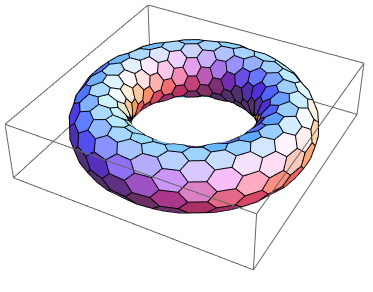
\includegraphics[width=0.75\textwidth]{images/test_image}
%	\caption{H-Mode Confinement Time Scaling} ~\\
%	\small This plot shows how well the ELMy H-Mode Scaling Law does for fitting $\tau_E$ to the ITER98 database of global tokamaks. For most values, the fit is at least 80\% accurate.
%	\label{fig:elmy}
%\end{figure}
%
%The use of the ELMy H-Mode scaling law also brings up another subtlety in the field. To measure the movement of energy within a plasma, scaling relations are needed that correlate to specific modes of plasma behavior -- i.e.\ ones that can robustly be found on a device by technicians. Currently, people rank H-Mode scalings over L-Mode ones (because H stands for high confinement and L stands for low). However, people often seek out other modes that can reliably be found on other machines. These go by names like: I-Mode (i.e.\ intermediate confinement), Enhanced H-Mode, and Reversed Shear modes. \cite{imode,enhanced,shear}
%
%Without going into too much detail, these alternate modes can be extremely valuable, as they often lead to more attractive reactors (than those made under H-Mode scalings). The problem, however, is often not finding a better performing mode on a single machine, but robustly finding it on other ones. This is important, because finding a mode on multiple machines is what allows new scaling relations to be produced and refined.\footnote{ In H-Mode and L-Mode's favor, they have been found on every machine that should see them. }

\section{Pricing a Fusion Reactor}

To \added{truly} compare tokamaks used as fusion \replaced{reactors, though,}{reactors} the obvious metrics are costs. ITER -- the \deleted{second} most expensive experiment \replaced{in the world\cite{nyt,bloomberg}}{today (only behind the LHC)} -- has a history \replaced{full of}{rich in} countries backing out for high \replaced{construction costs}{price tags} and rejoining only \replaced{after}{when} they finally get lowered.\cite{jeff} The problem is \$20B is a lot of money and 20 years is a long time. Moreover, approximating true costs \replaced{is difficult due to the}{becomes even trickier when designers} need to project (or neglect)  economies-of-scale for expensive components, such as the \added{superconducting} magnets and irradiated materials.

\replaced{Therefore,}{As such,} this paper adopts stand-ins for the conventional capital cost and cost-per-watt metrics. This is done for simplicity, \replaced{both in:}{for both:} \replaced{formulating the relations and}{modeling reasons as well as} conveying the two metrics to physicists. \replaced{The approximation for the}{To begin, the relevant approximation for} capital cost -- how much a tokamak costs to build -- is the magnetic energy. \cite{griffiths}
\begin{equation}
	\tcboxmath{
	W_M \propto R^3 B^2
	\label{eq:w_m}
	}
\end{equation}
\myequations{Magnetic Energy -- $W_M$}
In this magnetic energy proportion relation, the tokamak's major radius -- R -- is involved in a volumetric term ($R^3$) and B is the strength (in Teslas) of the \replaced{toroidal magnetic field.}{hooped shape magnetic field that lays nested within the plasma's shell (near its core).} This quantity simply states that the two surefire ways to make a machine more expensive \replaced{are to build it bigger and to use stronger magnets.}{to build are: making it larger and using stronger magnets.} \added{As these terms also improve confinement, this cost introduces a trade-off between size and magnet technology. This is why the proposed ARC reactor -- designed with HTS tape -- could be half the size of ITER, which uses conventional LTS technology.}

The next metric, the cost-per-watt, is defined by dividing the capital cost (i.e.\ the magnetic energy) by the main source of power output. \added{For a tokamak, this source of power is fusion -- discussed in more detail in \cref{chapter:power}.} \added{The cost-per-watt thus measures how economically competitive a reactor will be once it is build. This is how to compare the rate of return for different base-load power sources (e.g. fission, coal, and solar).} \deleted{This quantity measures how profitable a reactor will be once it is built. In a tokamak, the main power output is assumed to be fusion power, which relies on light elements (i.e.\ two Hydrogens) fusing into a heavier one (i.e.\ one Helium) -- hopefully releasing enough energy to offset the expense of causing it to happen in the first place. Although fusion power will not be defined till later, it does highlight the fact that this measure of cost-per-watt actually has units of time!}
\begin{equation}
	\tilde C_W = \frac{W_M}{P_F}
\end{equation}
\added{A final correction can be made on the cost-per-watt to account for reactor downtime, which is fundamental to pulsed operation. This is handled through the duty factor ($f_{duty}$) that is defined as the ratio of a reactor's quasi-steady-state flattop duration to the entire pulse length of a tokamak. In the context of the cost-per-watt, it scales down the fusion power:}
%\footnote{As energy per unit watt has units of time (i.e seconds).
\deleted{The final piece of the costing puzzle is a duty factor that levelizes the comparison of pulsed and steady-state tokamaks. As pulsed machines may be off 20\% of the time, their fusion power output should be reduced by that percentage. This is accounted for in the duty factor, which is simply the ratio of the flattop -- the time when pulsed machines are approximately held at steady-state -- to the entire length of the pulse.}
\deleted{In pulsed machines, the entire pulse includes charging the inductive sources as well as flushing out the tokamak between runs. These non-flattop portions of time can last around thirty minutes (where the reactor makes no money). As steady-state machines lack these non-flattop portions, their duty factors are rightfully one. Analysis in Fig.\ \ref{section:pulse} and discussion with several researchers, however, show that the same will probably hold true for a pulsed reactor, too.}
\deleted{Summarizing, the cost-per-watt coupled with the duty factor provides an ad hoc pricing metric, $C_W$, given by:}
\begin{equation}
	\tcbhighmath{
	C_W = \frac{W_M}{f_{duty} \cdot P_F}
	}
	\label{eq:c_w}
\end{equation}
\myequations{Cost-per-Watt -- $C_W$}
\added{For a steady-state reactor, this duty factor is assumed to be held at one. Pulsed machines, on the other hand, can see around thirty minutes of downtime,\cite{inputfile} which leads to duty factors around 80\%. Analysis in \cref{section:pulse}, however, shows that pulsed reactors may also have duty factors near unity.}

\deleted{It serves as a cornerstone for comparing the entire landscape of tokamak reactors -- whether they run in pulsed or steady-state operation. Although not a true engineering cost metric (i.e.\ in dollars per watt), it does provide an obvious physics meaning. Coupled with the magnetic energy stand-in for capital cost, these two costs allow researchers to pinpoint profitable and inexpensive tokamaks within reactor space.}

\added{Combined, these two cost metrics allow designers to pinpoint economically competitive tokamaks within reactor space. Although not rigorous in an engineering context, these capital cost and cost-per-watt approximations do provide true physics meaning while comparing different machines -- whether they run as pulsed or steady-state.}

\section{Modeling Fusion Systems}

Before reactors can be \replaced{priced}{costed}, though, they have to be modeled. Therefore the first half of this thesis is devoted to the theory behind tokamak design. \replaced{Emphasis}{A priority} is placed more on a physicist's intuition than an engineer's costing rigor. This is justified by the nonlinearities inherent to \deleted{the} fusion systems and rationalized by this paper's results matching more sophisticated \replaced{models}{frameworks} with high fidelity.

\added{Stepping back, a fusion systems model is an approach to designing reactors based on satisfying various physics and engineering constraints. There are many of these models in the field.\cite{hartmann,process,arc,minervini,helios,sycomore,fresco,aries,plasmod} Zero-dimensional (0-D) systems models are then a particular subclass of these that reduce the inherently 3-D problem of design to a collection of scalar, averaged values. This reduction in complexity allows models to be orders of magnitude faster. The natural corollary of this is that hundreds of reactors can be simulated in minutes.}

\added{Within the context of reactor design, these 0-D systems models serve an important role due to their speed and simplicity. Although not truly self-consistent,}\footnote{For speed concerns, 0-D fusion systems models often ignore self consistency in quantities like pressure profiles and use empirical fits to estimate values such as the confinement time.} \added{these models are capable of exploring large areas of reactor space. This is especially important in the early stages of tokamak planning when researchers are selecting a design point. These models also have use in finding general costing trends -- as shown in this document.}

What makes this paper's \added{systems} model different from \replaced{other ones, though,}{others in the field} is \replaced{its}{the} generalized handling of both modes of tokamak operation: pulsed and steady-state. This was necessitated by a desire to \added{fairly} compare the \replaced{two.}{two modes on a level playing field.} \replaced{The most fundamental result of this analysis is that both modes are actually capable of leading to economically competitive reactors}{What this shows is that both pulsed and steady-state tokamaks could make for profitable fusion reactors} -- assuming some technological advancements.

\section{Discussing HTS Magnet Technology}

\added{As mentioned, no economically competitive fusion reactor can be built using existing technology -- regardless of whether it runs as pulsed or steady-state. This is why MIT has been exploring HTS magnet technology for their ARC reactor in an effort to nearly double the maximum achievable field strength. What this paper shows is that this logic is indeed correct and HTS may be the final magnet advancement needed for the conventional fusion paradigm (i.e. D-T fuel, H-Mode, etc.)}

\deleted{One technological advancement that could lead to major wins is improving magnet components. This is why MIT has championed high-field designs for the better part of the last century. In their latest effort, the PSFC team has explored new high-temperature superconducting (HTS) tape capable of doubling the maximum achievable field strength. What this paper shows is that this logic is indeed correct and that HTS tape is all that is needed to build optimum reactors.}

More concretely, this paper shows that new HTS \deleted{tape} technology is capable of lowering \replaced{reactor costs -- both for pulsed and steady-state operation.}{both pulsed and steady-state tokamak costs.} \replaced{Further, this HTS tape has different uses within the two modes of operation -- as set by cost concerns (see \cref{fig:charybdis_intro,fig:proteus_intro}). This analysis shows that HTS should be employed in the TF coils for steady-state reactors \emph{and} in the central solenoid for pulsed ones. This is because pulsed machines require lower toroidal field strengths, which are achievable with less expensive LTS magnets.}{Further, the benefits of doubling the magnet strength bring the situation to a realm of significantly diminished rates of return. HTS is thus the end goal for the conventional D-T fusion paradigm.}

\deleted{Moreover, this model shows that HTS is best utilized in different components for pulsed and steady-state operation. Steady-state tokamaks favor HTS use in the D-shaped magnets that circle the machine (i.e.\ the TF coils). Whereas pulsed devices would benefit from employing HTS in the central solenoid -- that produces most of a reactor's inductive current. A corollary of this is the more conventional low-temperature superconducting (LTS) magnets (i.e.\ less expensive ones) can be used for pulsed TF coils, as their improved confinement levels off at much lower field strengths.}

Now that the problem has been thoroughly introduced, we will go over the theory behind steady-state and, then, pulsed tokamaks. A couple \replaced{detours}{segues} will be taken along the way to show how the model can be incorporated into a fusion systems code. This code -- Fussy.jl -- is the topic of \cref{chapter:fussy} and is freely available at:

{\centering \href{http://git.io/tokamak}{git.io/tokamak} \par } ~

\begin{figure*}[h]
    \centering
    \hfill
    \begin{subfigure}[t]{0.42\textwidth}
        \centering
    \begin{adjustbox}{width=\textwidth}
      \Large
      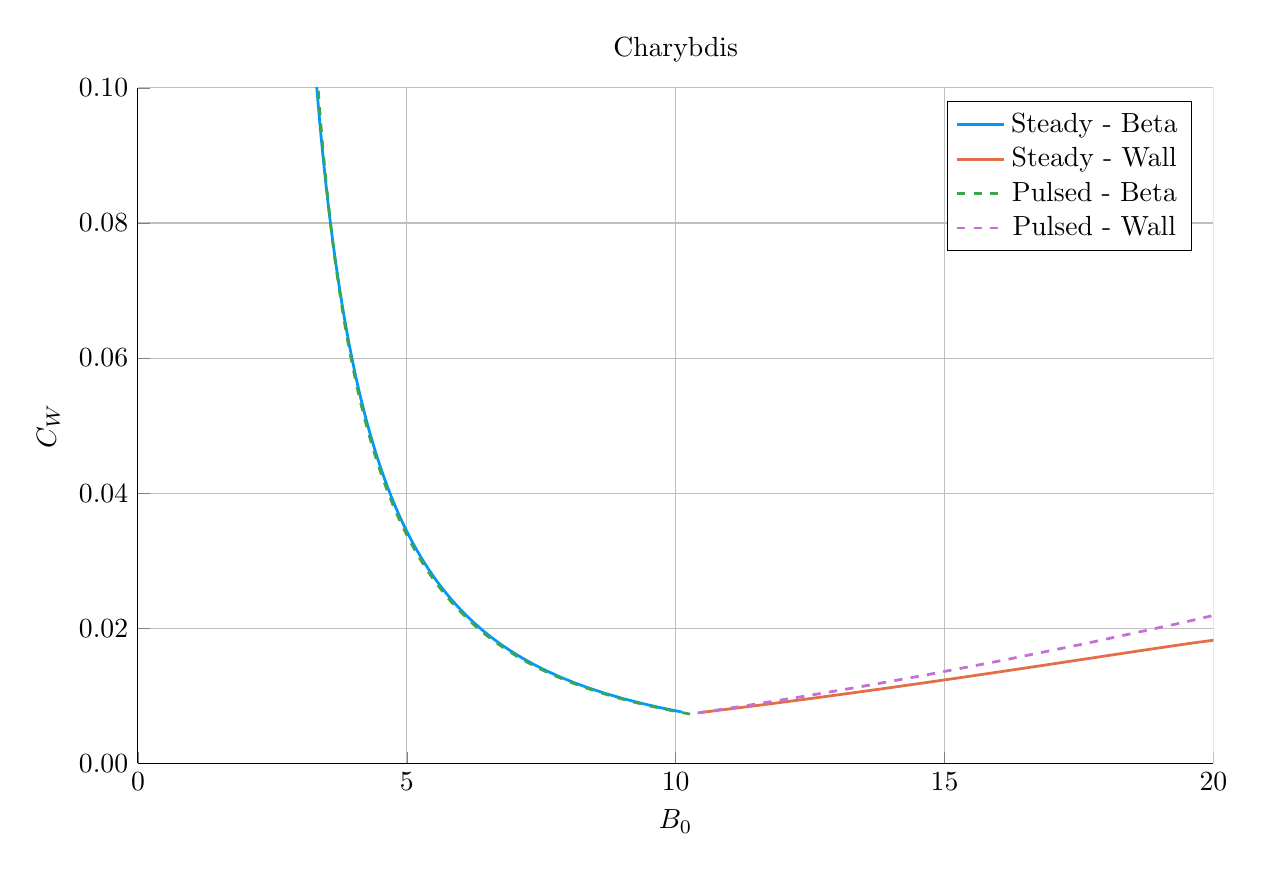
\begin{tikzpicture}[]
\begin{axis}[height = {101.6mm}, ylabel = {${C}_{W}$}, title = {Charybdis}, xmin = {0.0}, xmax = {20.0}, ymax = {0.1}, xlabel = {${B}_{0}$}, {unbounded coords=jump, scaled x ticks = false, xticklabel style={rotate = 0}, xmajorgrids = true, xtick = {0.0,5.0,10.0,15.0,20.0}, xticklabels = {0,5,10,15,20}, xtick align = inside, axis lines* = left, scaled y ticks = false, yticklabel style={rotate = 0}, ymajorgrids = true, ytick = {0.0,0.02,0.04,0.06,0.08,0.1}, yticklabels = {0.00,0.02,0.04,0.06,0.08,0.10}, ytick align = inside, axis lines* = left,     xshift = 0.0mm,
    yshift = 0.0mm,
    axis background/.style={fill={rgb,1:red,1.00000000;green,1.00000000;blue,1.00000000}}
, colorbar style={title=}}, ymin = {0.0}, width = {152.4mm}]\addplot+ [color = {rgb,1:red,0.00000000;green,0.60560316;blue,0.97868012},
draw opacity=1.0,
line width=1,
solid,mark = none,
mark size = 2.0,
mark options = {
    color = {rgb,1:red,0.00000000;green,0.00000000;blue,0.00000000}, draw opacity = 1.0,
    fill = {rgb,1:red,0.00000000;green,0.60560316;blue,0.97868012}, fill opacity = 1.0,
    line width = 1,
    rotate = 0,
    solid
}]coordinates {
(10.112818033153026, 0.007598383414978856)
(9.722156888543116, 0.008230424223188452)
(9.357875603858393, 0.008896404207575682)
(9.017653755630063, 0.009597023567402527)
(8.6995124437054, 0.010332804662622194)
(8.401566530516865, 0.011104394978990672)
(8.122163706328223, 0.011912345200844093)
(7.859819415455661, 0.012757161102175962)
(7.613196557650265, 0.013639302343912054)
(7.381088038653343, 0.014559181429827196)
(7.162401716104116, 0.015517162820285028)
(6.956147367527331, 0.016513562202290014)
(6.761425371986388, 0.017548645913683623)
(6.577416849463348, 0.018622630518712633)
(6.403375044688587, 0.019735682531644493)
(6.2386177769852695, 0.02088791828458706)
(6.0825208065966905, 0.022079403933712667)
(5.934511989185341, 0.02331015560822712)
(5.794066116682695, 0.024580139674436858)
(5.660700347012839, 0.02588927313954039)
(5.533970150598111, 0.027237424167073223)
(5.413465705416883, 0.02862441270831249)
(5.298808685607224, 0.03005001123436344)
(5.189649392059402, 0.031513945582432444)
(5.085664187259174, 0.033015895883282464)
(4.986553195072601, 0.03455549758379169)
(4.892038235455667, 0.03613234255000151)
(4.801860966679364, 0.037745980245626594)
(4.7157812114040425, 0.03939591897965519)
(4.633575445956479, 0.041081627216715676)
(4.5550354347559185, 0.04280253494397791)
(4.479966994069385, 0.04455803508845128)
(4.408188871204256, 0.046347484978679)
(4.33953172691477, 0.048170207844964834)
(4.273837210246432, 0.05002549435242988)
(4.210957116299974, 0.051912604161371986)
(4.15075261849161, 0.053830767509593334)
(4.0930935678432965, 0.05577918681155204)
(4.037857852672517, 0.05775703826940529)
(3.9849308127842145, 0.05976347349121981)
(3.9342047029103653, 0.06179762111185749)
(3.8855782007091695, 0.06385858841225403)
(3.838955955133626, 0.06594546293303978)
(3.7942481714200484, 0.06805731407868133)
(3.7513702293348077, 0.07019319470855978)
(3.710242331663442, 0.07235214271160313)
(3.6707891802306123, 0.0745331825613442)
(3.6329396770109583, 0.07673532684849063)
(3.5966266481325166, 0.07895757778829673)
(3.5617865887889004, 0.08119892870027327)
(3.5283594272686503, 0.08345836545794902)
(3.496288306480746, 0.08573486790664452)
(3.465519381509793, 0.08802741124736263)
(3.4360016318699595, 0.09033496738515884)
(3.4076866872513096, 0.0926565062404898)
(3.380528665662031, 0.09499099702224018)
(3.3544840229690007, 0.09733740946131986)
(3.3295114129297314, 0.09969471500383864)
(3.3055715568879336, 0.10206188796308927)
(3.2826271223788512, 0.10443790662966322)
(3.260642607548369, 0.10682175444066445)
(3.239584247604666, 0.10921242049746493)
(3.2194198921826622, 0.11160890156230109)
(3.2001189373344725, 0.11401020198268878)
(3.181652227422265, 0.11641533509457672)
(3.163991977015565, 0.11882332397376366)
(3.1471116955378684, 0.12123320224599504)
(3.130986116696265, 0.12364401485456963)
(3.115591132350856, 0.1260548187858383)
(3.1009037305081053, 0.12846468375306214)
(3.0869019371473265, 0.13087269283917113)
(3.0735647616124355, 0.13327794309901428)
(3.0608721453218655, 0.13567954612178545)
};
\addlegendentry{Steady - Beta}
\addplot+ [color = {rgb,1:red,0.88887350;green,0.43564919;blue,0.27812294},
draw opacity=1.0,
line width=1,
solid,mark = none,
mark size = 2.0,
mark options = {
    color = {rgb,1:red,0.00000000;green,0.00000000;blue,0.00000000}, draw opacity = 1.0,
    fill = {rgb,1:red,0.88887350;green,0.43564919;blue,0.27812294}, fill opacity = 1.0,
    line width = 1,
    rotate = 0,
    solid
}]coordinates {
(20.758867641064707, 0.018765308409143346)
(20.346250098246923, 0.018594952760163406)
(19.57104597888471, 0.01777146918538113)
(18.681781921115476, 0.016727851446155666)
(17.775790175980152, 0.015638576778075435)
(16.896654716492492, 0.014581653280825104)
(16.063927450323227, 0.013591211730165224)
(15.285557510665852, 0.012680275903338053)
(14.563500533069154, 0.01185123263968419)
(13.896568848875791, 0.01110114677254841)
(13.281970890030232, 0.010424581221258129)
(12.716170469467318, 0.009815118917575654)
(12.195372283741088, 0.00926617943914564)
(11.715794270833433, 0.008771443174384838)
(11.273815669498969, 0.008325054959037046)
(10.866051794088186, 0.007921704192505699)
(10.489365023931143, 0.007556609136513177)
};
\addlegendentry{Steady - Wall}
\addplot+ [color = {rgb,1:red,0.24222430;green,0.64327509;blue,0.30444865},
draw opacity=1.0,
line width=1,
dashed,mark = none,
mark size = 2.0,
mark options = {
    color = {rgb,1:red,0.00000000;green,0.00000000;blue,0.00000000}, draw opacity = 1.0,
    fill = {rgb,1:red,0.24222430;green,0.64327509;blue,0.30444865}, fill opacity = 1.0,
    line width = 1,
    rotate = 0,
    solid
}]coordinates {
(10.26788634689966, 0.007291637162809203)
(9.953967652326213, 0.007763018579561715)
(9.567926244368271, 0.008410560830066265)
(9.207974394987358, 0.009093056690349528)
(8.871841888699304, 0.009811202030777346)
(8.557505525932248, 0.010565644256199823)
(8.263156925406376, 0.01135697964954635)
(7.9871752024348766, 0.01218575089778548)
(7.728103682045175, 0.013052444820635726)
(7.484629973620137, 0.01395749030938975)
(7.255568856523303, 0.014901256485610468)
(7.039847526735421, 0.015884051087442074)
(6.836492834698909, 0.01690611908975986)
(6.644620209081183, 0.01796764156282338)
(6.463424013335149, 0.01906873477252413)
(6.2921691243175495, 0.020209449523749864)
(6.13018355681404, 0.02138977074682875)
(5.97685198655569, 0.022609617323612653)
(5.831610044919842, 0.023868842161338135)
(5.693939286027163, 0.025167232481888336)
(5.563362729090489, 0.026504510357656302)
(5.439440906144732, 0.0278803334592314)
(5.321768347746793, 0.02929429601917866)
(5.209970453003084, 0.030745929990983068)
(5.103700692769835, 0.03223470641747899)
(5.002638109938164, 0.03376003696406285)
(4.906485077678376, 0.03532127563010485)
(4.814965286571576, 0.03691772061565451)
(4.727821933804548, 0.03854861633202897)
(4.644816091323922, 0.04021315554278132)
(4.565725232806084, 0.04191048162126061)
(4.490341901840154, 0.04363969091085349)
(4.418472505906755, 0.04539983517396531)
(4.349936222622964, 0.047189924115870814)
(4.284564006352339, 0.049008927969770806)
(4.222197684694192, 0.05085578012965056)
(4.162689135592264, 0.05272937981792158)
(4.105899536872315, 0.05462859477526984)
(4.051698680949713, 0.056552263960658246)
(3.9999643482627323, 0.058499200250012214)
(3.9505817337017928, 0.06046819312273483)
(3.903442920928527, 0.062458011325916454)
(3.858446400032002, 0.06446740550676137)
(3.8154966244515616, 0.06649511080452623)
(3.7745036035252744, 0.06853984939399767)
(3.7353825273991994, 0.07060033297331114)
(3.6980534213689746, 0.07267526518964869)
(3.6624408270205375, 0.07476334399712868)
(3.62847350780097, 0.07686326394192533)
(3.5960841768845415, 0.07897371837037194)
(3.565209245407392, 0.08109340155652811)
(3.5357885893311605, 0.0832210107463015)
(3.5077653333614305, 0.08535524811591486)
(3.4810856504959875, 0.08749482264305544)
(3.4556985759109375, 0.08963845188964095)
(3.4315558340122845, 0.09178486369563649)
(3.408611677587535, 0.09393279778385825)
(3.3868227380888998, 0.09608100727612065)
(3.36614788616562, 0.09822826012150637)
(3.3465481016421226, 0.10037334043786662)
(3.327986352208224, 0.1025150497680155)
(3.3104274769652595, 0.10465220838353721)
(3.2938380965241474, 0.1067836557197021)
(3.278186482171801, 0.10890825269906537)
(3.263442495132517, 0.11102488135374605)
(3.2495774839156075, 0.1131324463411963)
(3.236564206241785, 0.11522987560063444)
(3.224376752844934, 0.11731612107126856)
(3.212990475972638, 0.11939015934381376)
(3.2023819222517877, 0.12145099224802183)
(3.192528769611062, 0.12349764737898258)
(3.1834097679780142, 0.1255291785649034)
(3.1750046834890777, 0.12754466627907632)
(3.1672942459724482, 0.12954321799866983)
};
\addlegendentry{Pulsed - Beta}
\addplot+ [color = {rgb,1:red,0.76444018;green,0.44411178;blue,0.82429754},
draw opacity=1.0,
line width=1,
dashed,mark = none,
mark size = 2.0,
mark options = {
    color = {rgb,1:red,0.00000000;green,0.00000000;blue,0.00000000}, draw opacity = 1.0,
    fill = {rgb,1:red,0.76444018;green,0.44411178;blue,0.82429754}, fill opacity = 1.0,
    line width = 1,
    rotate = 0,
    solid
}]coordinates {
(48.990476413653056, 0.09724163307501366)
(42.83950920694117, 0.07766994779263652)
(37.687790427214495, 0.06269593244609177)
(33.33937742845888, 0.05109841711622891)
(29.64296398154308, 0.04201539110057761)
(26.48039367255613, 0.034828857187910324)
(23.758442882319894, 0.029089432591006322)
(21.402860298405816, 0.02446606951047545)
(19.353987387634486, 0.020711961258999954)
(17.563502020363714, 0.017641064746807725)
(15.991970371213752, 0.015111701839397276)
(14.606987499719377, 0.013014953187280779)
(13.381751501116137, 0.011266342778060628)
(12.293960329570087, 0.009799811915435606)
(11.32495111804522, 0.00856330563618739)
(10.459023415380802, 0.007515507834648486)
(10.26788634689966, 0.007291637162809203)
};
\addlegendentry{Pulsed - Wall}
\end{axis}

\end{tikzpicture}

    \end{adjustbox}
        \caption{Toroidal Field Sensitivity}
    \end{subfigure}
    \hfill
    \begin{subfigure}[t]{0.48\textwidth}
        \centering
    \begin{adjustbox}{width=\textwidth}
      \Large
      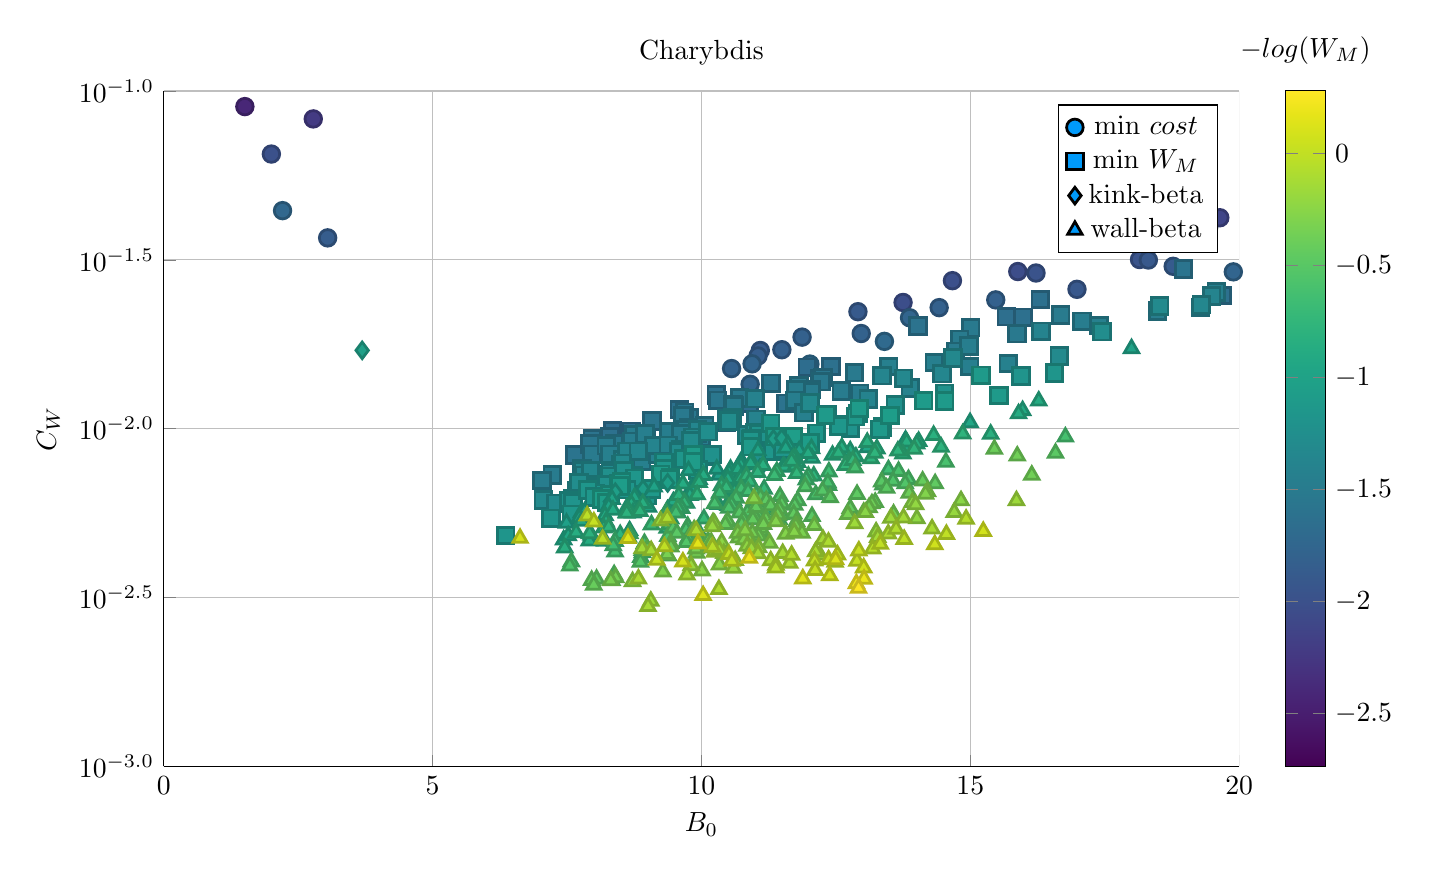
\begin{tikzpicture}[]
\begin{axis}[colorbar = {true}, height = {101.6mm}, ylabel = {${C}_{W}$}, title = {Charybdis}, xmin = {0.0}, xmax = {20.0}, ymax = {0.1}, ymode = {log}, xlabel = {${B}_{0}$}, {unbounded coords=jump, scaled x ticks = false, xticklabel style={rotate = 0}, xmajorgrids = true, xtick = {0.0,5.0,10.0,15.0,20.0}, xticklabels = {0,5,10,15,20}, xtick align = inside, axis lines* = left, scaled y ticks = false, yticklabel style={rotate = 0}, log basis y=10, ymajorgrids = true, ytick = {0.001,0.0031622776601683794,0.01,0.03162277660168379,0.1}, yticklabels = {$10^{-3.0}$,$10^{-2.5}$,$10^{-2.0}$,$10^{-1.5}$,$10^{-1.0}$}, ytick align = inside, axis lines* = left,     xshift = 0.0mm,
    yshift = 0.0mm,
    axis background/.style={fill={rgb,1:red,1.00000000;green,1.00000000;blue,1.00000000}}
, colormap={plots}{rgb=(0.26700400,0.00487400,0.32941500), rgb=(0.27794100,0.05632400,0.38119100), rgb=(0.28291000,0.10539300,0.42690200), rgb=(0.28229000,0.14591200,0.46151000), rgb=(0.27619400,0.19007400,0.49300100), rgb=(0.26514500,0.23295600,0.51659900), rgb=(0.25042500,0.27429000,0.53310300), rgb=(0.23360300,0.31382800,0.54391400), rgb=(0.21813000,0.34743200,0.55003800), rgb=(0.20123900,0.38367000,0.55429400), rgb=(0.18555600,0.41857000,0.55675300), rgb=(0.17117600,0.45253000,0.55796500), rgb=(0.15772900,0.48593200,0.55801300), rgb=(0.14618000,0.51541300,0.55682300), rgb=(0.13374300,0.54853500,0.55354100), rgb=(0.12346300,0.58168700,0.54744500), rgb=(0.11948300,0.61481700,0.53769200), rgb=(0.12632600,0.64410700,0.52531100), rgb=(0.15014800,0.67663100,0.50658900), rgb=(0.19109000,0.70836600,0.48228400), rgb=(0.24607000,0.73891000,0.45202400), rgb=(0.31192500,0.76782200,0.41558600), rgb=(0.37777900,0.79178100,0.37793900), rgb=(0.45867400,0.81636300,0.32972700), rgb=(0.54552400,0.83803900,0.27562600), rgb=(0.63690200,0.85654200,0.21662000), rgb=(0.73088900,0.87191600,0.15602900), rgb=(0.81457600,0.88339300,0.11034700), rgb=(0.90631100,0.89485500,0.09812500), rgb=(0.99324800,0.90615700,0.14393600)}, colorbar style={title=$-log( W_M )$}}, ymin = {0.001}, width = {152.4mm}]\addplot+[scatter, scatter src=explicit, only marks = {true}, color = {rgb,1:red,0.00000000;green,0.60560316;blue,0.97868012},
draw opacity=1,
line width=0,
solid,mark = *,
mark size = 3.0,
mark options = {
    color = {rgb,1:red,0.00000000;green,0.00000000;blue,0.00000000}, draw opacity = 1.0,
    fill = {rgb,1:red,0.00000000;green,0.60560316;blue,0.97868012}, fill opacity = 1,
    line width = 1,
    rotate = 0,
    solid
}] coordinates {
(43.17364371307109, 0.20372611777337152) [-2.737608795379803]
(36.93734773821979, 0.16756698485075783) [-2.687028959846787]
(48.32519073723288, 0.20307732356386315) [-2.590964172611572]
(27.818653653131317, 0.09697011319422226) [-2.5133293798402634]
(24.031609210800628, 0.08246486806905176) [-2.5100019193902536]
(46.9757183374081, 0.19848215388453824) [-2.5025824444647777]
(45.280165981821085, 0.18469850991270712) [-2.5011605733960924]
(34.33588556676648, 0.12156262800516612) [-2.487146433631915]
(49.350050230883724, 0.19851381203738652) [-2.4809660057819647]
(47.77223182347582, 0.18516332132320687) [-2.470276837036607]
(1.509009505191671, 0.08989325143911144) [-2.4120510478783452]
(1.607785753409308, 0.11208716242840429) [-2.40064821683863]
(36.7130287359324, 0.1197463715660703) [-2.3953673323479805]
(1.8837521570225992, 0.16126185747296792) [-2.393026566903574]
(40.03911031913926, 0.12157790627296668) [-2.3890711431592075]
(29.797147437037797, 0.08892691625963052) [-2.3841714318705525]
(49.837627165397436, 0.19098420146344375) [-2.3835230043455686]
(44.09667775143585, 0.1567069747417994) [-2.381290315955617]
(40.10027193508949, 0.12013460973440174) [-2.372431680776573]
(49.50704240080035, 0.18909730733563926) [-2.3528250340145016]
(28.968881363864583, 0.09075329244454268) [-2.3367870360584306]
(42.98831457790196, 0.14161197175057597) [-2.321478568273318]
(20.175934198309292, 0.05204568902739023) [-2.305558880403713]
(39.444164493588694, 0.12356138844469775) [-2.304074016625784]
(18.58289304393365, 0.04451265485552352) [-2.302767677581907]
(48.357898732015734, 0.16063854506387298) [-2.296827704935537]
(37.45895333311772, 0.10163604971512134) [-2.2875898578722627]
(38.208044910992896, 0.11621384520807569) [-2.277792210835674]
(48.821328515678495, 0.1663671711858832) [-2.2429196737605452]
(44.47436973980107, 0.14065371048755002) [-2.2307023150334016]
(36.201327387935265, 0.0992781716492562) [-2.229928759421221]
(24.976048511930994, 0.06165765133592798) [-2.225497521252979]
(2.781115265361342, 0.08264995845897197) [-2.2254079847151558]
(38.524798940282565, 0.10066936171865973) [-2.2222117952587324]
(40.75335661697331, 0.11283696845057267) [-2.2164511971368666]
(31.550557574122383, 0.07858675141449649) [-2.209080463460292]
(22.187409115367732, 0.055353669168383704) [-2.209072102647127]
(30.40343222814581, 0.08246628156983182) [-2.2082284492074966]
(22.891943050812795, 0.05534045927382465) [-2.207545754633005]
(32.48318348912026, 0.0812523499942961) [-2.2073960717358423]
(20.46108539491903, 0.04959003498021099) [-2.1906798686881843]
(24.303991155057293, 0.058916370946488036) [-2.180354292184896]
(20.69670598282277, 0.04458441983079472) [-2.1445063804884623]
(23.83667769146755, 0.05969099272190574) [-2.1441459472897755]
(19.63958505006771, 0.04213154094480493) [-2.1211539010866085]
(40.900769162095195, 0.11416954810746238) [-2.118865769548717]
(21.37751157855586, 0.04953083435602705) [-2.0989534800462293]
(33.36930679768429, 0.08867461574773429) [-2.098220502653117]
(24.013965403457117, 0.0528553369774306) [-2.0935531757786148]
(22.393434928615605, 0.05131047258257683) [-2.0908793980048204]
(29.571629059289982, 0.06966107994211436) [-2.071206080374841]
(20.977574074646927, 0.03996425224364798) [-2.064010547202469]
(18.060179054192336, 0.03708750697043753) [-2.056677518407323]
(35.94446843645834, 0.08410248770893317) [-2.046651526754166]
(15.882761260039363, 0.029196081498388402) [-2.0379011758864283]
(30.46355269165919, 0.07740613615195041) [-2.0346098603711273]
(13.74929111510663, 0.023645385119135078) [-2.0286798881208097]
(14.667163745602908, 0.027435451545116674) [-2.0136110022221563]
(40.970645504124256, 0.11225395679162868) [-2.009422091461703]
(18.86549676786543, 0.038038514881495206) [-2.0046094254929896]
(2.0018449519379766, 0.06504727548043324) [-1.9998626026906214]
(1.333016896105282, 0.1292818470624988) [-1.994011891463306]
(16.221280003397087, 0.028908830411030862) [-1.9684875514336135]
(18.146839242470875, 0.031694615819844695) [-1.962505769886516]
(20.536616448979608, 0.041976164443053174) [-1.9620022465602456]
(26.5908410355429, 0.0558374666834525) [-1.9556964151982232]
(24.564582250767256, 0.051180643617204404) [-1.951439472922028]
(19.431812066409112, 0.03938689654476367) [-1.9407104232831573]
(26.69111333219166, 0.05202238389928039) [-1.9285131737739916]
(16.98328208989546, 0.025864965787053298) [-1.9158089273231942]
(18.310414889815103, 0.0315876708787529) [-1.9026235632381945]
(23.297584692796203, 0.04007799426592172) [-1.8998797107494547]
(31.023963052023834, 0.06078277028813781) [-1.899469008660825]
(12.910038525246692, 0.022206649532263138) [-1.8922403969034376]
(41.62061738174131, 0.10343738795419383) [-1.8906275193753241]
(20.52842536101005, 0.03865878413437627) [-1.888904730447693]
(11.094220133483955, 0.01704724215883986) [-1.881726038777211]
(26.82066656529518, 0.05468787224768575) [-1.8763775212700056]
(35.10552519829791, 0.06894730353059726) [-1.8735628617782005]
(18.772509744848122, 0.030255781340376833) [-1.8728583861908288]
(27.360822192582077, 0.05616340524751281) [-1.8726476950037667]
(24.81797703498571, 0.04508699905590542) [-1.8707673950160981]
(3.0483538111563147, 0.036730885786441146) [-1.8559040168248113]
(29.522060018630928, 0.06072120698828991) [-1.844735439552174]
(39.46604489934323, 0.0887876180917983) [-1.8430067319432535]
(36.423170296938046, 0.06618962633184258) [-1.8418706711323614]
(11.051798631687303, 0.016421469596061083) [-1.839654971931263]
(25.458813886025002, 0.041749778425302704) [-1.8363695553529753]
(11.495131548398012, 0.017133631996777206) [-1.8261042714032643]
(32.71889711711922, 0.06559232169922954) [-1.8156007183182272]
(27.372160767771714, 0.050477285906930965) [-1.814915147975814]
(25.58270520703581, 0.0463768454249938) [-1.8142470512570916]
(14.420380568742246, 0.022826470712123872) [-1.8122133933822206]
(11.871194516454642, 0.018671308945999422) [-1.8120480447424478]
(15.472612894867664, 0.02406843511337114) [-1.810457309558868]
(20.542658667696518, 0.03627504764978015) [-1.8068853182048894]
(12.97099575986033, 0.019138039216325595) [-1.8019457667366159]
(21.252479627137433, 0.03724912279904193) [-1.7968505393892884]
(10.560232043643675, 0.015068032824050809) [-1.7952329403066731]
(45.12856703204009, 0.10460346899306477) [-1.7847262081815998]
(42.21258282310005, 0.09611727933154134) [-1.7840094275762153]
(13.869520871341438, 0.021310065419317785) [-1.76773605949338]
(19.89092632819806, 0.02913495659310822) [-1.7643358761825505]
(10.905382526033923, 0.013537430460188857) [-1.7636964772599824]
(10.941389456318912, 0.015563838196545969) [-1.7631697711543228]
(22.454106310710905, 0.039135813481222324) [-1.7625125196445544]
(30.835040451521607, 0.058991966200443106) [-1.7573515468471756]
(2.20974763812607, 0.04422563848495237) [-1.7287980416000448]
(38.02614384410885, 0.07767888704178068) [-1.7234251960549989]
(32.76556364087757, 0.06204137364185275) [-1.706346162862732]
(13.40240917641803, 0.018138423087163798) [-1.7045486732225623]
(46.55916074836906, 0.09124971330207729) [-1.7014359592573747]
(22.042270993490888, 0.0365316783828158) [-1.6927990438723723]
(12.016385149605648, 0.015536674756802697) [-1.6898457437353114]
(24.29682482728058, 0.04003550886686569) [-1.6732846842044926]
};
\addlegendentry{min $cost$}
\addlegendentry{min $W_M$}
\addlegendentry{kink-beta}
\addlegendentry{wall-beta}
\addplot+[scatter, scatter src=explicit, only marks = {true}, color = {rgb,1:red,0.00000000;green,0.60560316;blue,0.97868012},
draw opacity=1,
line width=0,
solid,mark = square*,
mark size = 3.0,
mark options = {
    color = {rgb,1:red,0.00000000;green,0.00000000;blue,0.00000000}, draw opacity = 1.0,
    fill = {rgb,1:red,0.00000000;green,0.60560316;blue,0.97868012}, fill opacity = 1,
    line width = 1,
    rotate = 0,
    solid
}] coordinates {
(11.967738248169791, 0.015197399614753464) [-1.6681264025020264]
(8.696464418773537, 0.009823451646161325) [-1.663027891651841]
(8.345089297998298, 0.009846202245989184) [-1.6574639825902946]
(10.880655338826603, 0.011920058291303071) [-1.6569597902573525]
(44.33631295480244, 0.07535163980234072) [-1.6567719329389001]
(15.669504585643491, 0.02145281320442147) [-1.6490985707391912]
(10.539028948810953, 0.010980468278747128) [-1.6422304847233504]
(16.300333423271717, 0.024120165421292625) [-1.6325751861823363]
(15.984439076117749, 0.021369208393676346) [-1.6291941426087102]
(32.92820758192895, 0.059322254561326254) [-1.6271960977249518]
(12.410293143428914, 0.015274978962504819) [-1.6270750467611084]
(19.688988499386202, 0.02479273110440336) [-1.626888156587228]
(47.183683314686505, 0.08930149237460469) [-1.6249314455189936]
(8.292561647347492, 0.009464726031912818) [-1.616950986036806]
(9.588347137721799, 0.01140193486941599) [-1.6155813119347568]
(8.006641138103518, 0.008812988458667981) [-1.6136190879018757]
(39.148691259933166, 0.06439016913414505) [-1.6120765470743166]
(10.27384306214681, 0.012585512817446045) [-1.6084381516776733]
(14.028211695717372, 0.02012839274260647) [-1.6020711217447665]
(7.943473491980901, 0.008960652359910951) [-1.5956625490662]
(11.571557791481624, 0.011885919211945236) [-1.5936419030965376]
(21.806471384188846, 0.03445722055743375) [-1.591719437101271]
(7.968648039596557, 0.00935259758229712) [-1.5882416690043395]
(8.97123185854356, 0.00941739351173858) [-1.587943800614445]
(7.642159237594249, 0.008359730036220061) [-1.5878025494857624]
(10.460983583083753, 0.010419937829338555) [-1.5868755906181577]
(18.965059522862617, 0.029697190504060857) [-1.5849823271963874]
(12.194568732238995, 0.014090253789926491) [-1.5820661333237485]
(9.813866298873991, 0.009872769680224545) [-1.571414774494934]
(24.25469890895016, 0.036055486397936085) [-1.561587842338199]
(8.517935684154212, 0.009008401602884603) [-1.5604752308741954]
(9.080862100268657, 0.010548811329102839) [-1.560024208321792]
(9.789660341943907, 0.00975086483062938) [-1.5595172183929409]
(8.133164457566973, 0.008877515881031174) [-1.5547403592804268]
(10.297704899446542, 0.012128004524771618) [-1.5525172912757694]
(9.766479902832291, 0.01075120106159998) [-1.550211325130473]
(12.2632951302657, 0.01417054313300387) [-1.5499921130488996]
(11.291662119925611, 0.013636547782905628) [-1.5488389310082484]
(9.686757381363082, 0.01118682853182229) [-1.548636584215126]
(7.924713370279235, 0.009004515948176011) [-1.5484303677563682]
(8.54226502879131, 0.008589361734950092) [-1.5300696832010154]
(9.64758141032686, 0.010918478084483) [-1.5240418415006989]
(12.21993539420707, 0.013786535741271849) [-1.52035115860342]
(15.867234965970042, 0.019102159289939535) [-1.5187095286365286]
(15.007125908258939, 0.019900882686515825) [-1.5152558703618486]
(10.70858947114034, 0.01233142370653334) [-1.5130633149050525]
(8.529805552034778, 0.008998649144966384) [-1.5127417843169062]
(8.377294862413901, 0.009033035828776036) [-1.512065872282441]
(12.846715954681153, 0.014648425212785676) [-1.508698938344436]
(16.682126583618288, 0.021717369003602268) [-1.5042599211378067]
(10.58390997110411, 0.011787983533386965) [-1.5034350531454859]
(11.810966417691285, 0.013402736400337721) [-1.50170709764633]
(7.965952597674263, 0.008403497514698337) [-1.501622468932281]
(12.052123659751864, 0.013038942564365743) [-1.5014482706318735]
(14.803678461986678, 0.018390392389316428) [-1.4999954524234758]
(14.727306928855038, 0.01694354359189593) [-1.4973617780251773]
(10.061864920509048, 0.010183371556613061) [-1.497105465512374]
(40.24136746900709, 0.062282935043912684) [-1.4929511344473714]
(41.49663881325739, 0.06324187033686292) [-1.4921349419619385]
(11.804455973082419, 0.012548762978995496) [-1.4884591559674822]
(12.029939715648373, 0.012867101009559307) [-1.487363796795517]
(12.601637635718813, 0.012921001622500157) [-1.4866917975345906]
(9.754197703405268, 0.010047951074758055) [-1.4840978906845892]
(21.882416551144317, 0.03303866433608294) [-1.4824521913249147]
(12.942504869667264, 0.012726704506142847) [-1.4821332841886103]
(7.226740691315094, 0.007290805739373347) [-1.48122389777201]
(9.72526998487911, 0.00977012454088988) [-1.4804970319589599]
(7.032760703447595, 0.007020834402326414) [-1.4800609203732897]
(8.228283040534254, 0.008910343679206711) [-1.4785263901161534]
(11.757080569358145, 0.013060328514041545) [-1.4759327339004988]
(8.742108415330497, 0.009568901799246174) [-1.4716802129865878]
(10.608355718332808, 0.011686646580567617) [-1.4714171457200942]
(10.002017917096252, 0.009432683201513142) [-1.4697490463241623]
(17.076056816605465, 0.0207896268155257) [-1.469182095495403]
(9.93096524460024, 0.00970055448692835) [-1.4669160574764228]
(9.646537177073283, 0.009906198335664992) [-1.4650279037766998]
(8.492788974520707, 0.008175296861755412) [-1.4649157170050158]
(39.01795702656691, 0.06304537805517052) [-1.4637589731711664]
(37.319780376430465, 0.058293696935902015) [-1.4637269213699509]
(18.482121616159016, 0.022332692478256824) [-1.4633431723635995]
(8.698182291263416, 0.009175072172052877) [-1.4625771233357587]
(28.127107238558466, 0.03507245292213848) [-1.4624493219359893]
(24.405556044324065, 0.0323252483349636) [-1.456137936078477]
(11.740431759483823, 0.012144991566364045) [-1.4552956920106896]
(9.39566274467647, 0.009807429458519862) [-1.4545765412204814]
(14.971887946904854, 0.017552109366812733) [-1.4536933205355047]
(8.340793691955412, 0.008376880643338882) [-1.4536264367612777]
(20.758621662871732, 0.027928446404318328) [-1.4522195766945736]
(14.989566420933915, 0.015275332383460013) [-1.4474663709891824]
(14.328449262483707, 0.015700047070746036) [-1.4473086055649607]
(9.614108815012006, 0.009670159078421467) [-1.4394573389116623]
(8.946816680478415, 0.00966580645268258) [-1.43910869750835]
(17.39032103778615, 0.02020398851625505) [-1.4359212547397637]
(8.887301811416945, 0.008025741974410725) [-1.4345455569874563]
(8.293678413022477, 0.008395971364345037) [-1.4342039611389994]
(34.870157215661116, 0.055516720625521446) [-1.431939711468657]
(9.215949656599236, 0.008564631451482608) [-1.4318393301192203]
(13.483733389139449, 0.015286328537971657) [-1.4298782830268841]
(11.909294643223976, 0.011144326549623773) [-1.4297531319990848]
(19.28479299500749, 0.022836013108600235) [-1.429493152311542]
(19.574343065749268, 0.02541733792453219) [-1.4257656907023994]
(7.775559573362513, 0.007637958943877289) [-1.4246908118870814]
(25.190615990519625, 0.032702505993041836) [-1.4223151615986427]
(15.706222639321235, 0.015605848032644089) [-1.4209285260987674]
(9.186736487920959, 0.00838874188644035) [-1.4103191250155003]
(7.810243176708771, 0.007287678962320866) [-1.409160412241362]
(10.994509564269785, 0.012263516831132143) [-1.3987487890322283]
(11.014663159593116, 0.010656632838165833) [-1.3961077718749653]
(13.882977876787413, 0.013186567390631069) [-1.39553831950318]
(9.36196654538676, 0.00805251109990194) [-1.3921916689745937]
(16.3128197434878, 0.019423304332311736) [-1.391977480132208]
(21.05130093390351, 0.025114205055596032) [-1.3910450519688433]
(21.18381811006707, 0.026458278303411537) [-1.3854794296349102]
(13.100755547904486, 0.012247975078154037) [-1.3835251244626703]
(9.120715613380417, 0.008921077760690099) [-1.3812630274600655]
(7.896894254399229, 0.007416332681742631) [-1.3791460184166777]
(9.381274310380604, 0.008932161350486465) [-1.376877777579119]
(19.488100600993267, 0.024683476432383993) [-1.375791428631395]
(10.475402655568338, 0.010670268336180793) [-1.3747828318073587]
(9.32515552589659, 0.007870433585163046) [-1.3692376523933565]
(7.9286970308329465, 0.0074378152848894735) [-1.3684330757581267]
(8.538214357510187, 0.008098566001726598) [-1.3642308788975135]
(13.354119232582212, 0.014345667909698757) [-1.3639106630352087]
(8.608422674568363, 0.008572986953587419) [-1.3552608297970883]
(9.925761115396522, 0.00992037446225701) [-1.3550143961305745]
(8.004082331921554, 0.007328347073490059) [-1.3536632792649093]
(7.802422783894211, 0.007510901593863939) [-1.3520272957429909]
(14.471041037539871, 0.014541602438699657) [-1.3510576974042412]
(7.810600769649848, 0.007284218364658594) [-1.3496042220443973]
(19.296422276685288, 0.023274179527198832) [-1.341589260669594]
(8.824939461101431, 0.008576558289309913) [-1.3400141478767358]
(8.49764138867205, 0.00783880949696723) [-1.3300314493551002]
(13.758392145064837, 0.01411038207207742) [-1.3284263237560021]
(7.937511343586117, 0.007486503783717723) [-1.3242939338468662]
(14.679707952711722, 0.016172436730796002) [-1.323178727777929]
(8.319781298347303, 0.007515284989600465) [-1.3213550729926942]
(27.500324284476235, 0.031083172357107024) [-1.3188753969554132]
(7.672777169827471, 0.006572813918743706) [-1.3138992633454782]
(34.26204390685552, 0.04309583371292883) [-1.3112533972207423]
(8.305241116382918, 0.007413444843148486) [-1.3066175516543825]
(18.522037273131268, 0.02306836377257982) [-1.3040612288627607]
(9.843274954742599, 0.00943254285754032) [-1.3038133693852783]
(12.01595379328233, 0.01190899263404481) [-1.301084703290134]
(8.530188695097733, 0.00789699984651379) [-1.3010145120900876]
(7.059381386127842, 0.006149219434619409) [-1.3000605956773916]
(16.655180883583878, 0.016437005811172183) [-1.2981699890610565]
(9.606246685298759, 0.008660055713531614) [-1.2951558801969907]
(10.571439501867458, 0.010749954823506654) [-1.29444309797184]
(7.284894188691189, 0.006015009649024556) [-1.2856101424882644]
(10.842752178226151, 0.009584357937856927) [-1.285263592011844]
(34.353143867925155, 0.04494124949431044) [-1.284383793501614]
(7.905156667937178, 0.00683431321635412) [-1.2828114288158374]
(31.635765029342274, 0.039187382342347976) [-1.2826431650359629]
(8.313601928775393, 0.007231700278305266) [-1.2824255065429995]
(9.578913894726805, 0.00853616645957665) [-1.2813323109549335]
(7.924882086401339, 0.006837657402697755) [-1.2806421539894215]
(9.808329366529762, 0.009211465915111147) [-1.2790915578265545]
(10.511748242466084, 0.010542099378207213) [-1.2707451840708122]
(23.70716861300546, 0.024447750750697092) [-1.2676539939434082]
(11.00520478529279, 0.009098409772603787) [-1.2653553126366786]
(7.876105123562427, 0.006725537497980498) [-1.264293982211982]
(17.45204956258683, 0.019363431367524053) [-1.262045130852001]
(7.719844293445014, 0.006906076996276599) [-1.2611290819783112]
(10.118399421716713, 0.009803145458874337) [-1.2555987795426622]
(7.612390232156273, 0.00619895569247597) [-1.2513270179335647]
(8.729387536492673, 0.007239853513876978) [-1.2453167838780697]
(10.961169543919764, 0.008896586162085272) [-1.2430939343579344]
(10.985358154781366, 0.009719593902466845) [-1.2381773742332136]
(10.055825077383927, 0.008270424440644015) [-1.2346782486332617]
(8.291481327682558, 0.0072241626571935376) [-1.2264046023709216]
(12.335638193913455, 0.01098843719538726) [-1.2247195887884887]
(8.246208566536797, 0.006808974225612837) [-1.2180889658059086]
(8.540264952931636, 0.006611305121542242) [-1.2173874089477876]
(8.556190004184526, 0.007501419726936573) [-1.2146247722956514]
(13.602894240173864, 0.011764386053045915) [-1.2132972156104522]
(10.195221885432844, 0.008378063320530003) [-1.2109120215395388]
(11.049738848862685, 0.008427299987451904) [-1.2084181738286368]
(14.519807280009873, 0.01273555061242485) [-1.20714909048448]
(12.595222602654314, 0.010213320377511352) [-1.2033520253557135]
(26.383495577820405, 0.032086426450625864) [-1.1973567207367808]
(12.639134913781255, 0.01024990923611188) [-1.1946911954531152]
(12.771017041564328, 0.010020735618058307) [-1.194687477055283]
(11.065493657555185, 0.009634752809511687) [-1.1937967228670217]
(15.93895045303613, 0.014319974319254046) [-1.185724861965876]
(28.62771924607459, 0.030946696104817876) [-1.1815951507377263]
(7.535456478096903, 0.006119538485938838) [-1.1806237088701466]
(7.610400378886139, 0.0060467130253046425) [-1.1800813312023146]
(9.303943294896706, 0.007952378649071718) [-1.176244530950471]
(8.033169581940832, 0.006432608194369421) [-1.1748225292203367]
(7.199323628519372, 0.005427058328431804) [-1.1721208310483742]
(8.635658099111911, 0.006744537821609478) [-1.1717373686057835]
(6.357367087501427, 0.004828891223049449) [-1.1708649361692889]
(8.68097527641003, 0.006810003648499363) [-1.1692163263768098]
(10.941107168878954, 0.009353534353065332) [-1.167353919317699]
(16.564321004099757, 0.014618785296867573) [-1.1652399164280889]
(11.54197585545895, 0.008829535690276422) [-1.162809974145342]
(8.753893841415247, 0.007136024429485349) [-1.1600693635040116]
(7.885243678455898, 0.006579111152003091) [-1.157321108695414]
(11.32266327338597, 0.008599780741533768) [-1.1572067562856314]
(10.915418141745553, 0.009251618906581017) [-1.1571634670399211]
(9.667898706541429, 0.008133610271699837) [-1.154357334346231]
(12.910014006891455, 0.011084851654264415) [-1.1506586644938104]
(11.51111009989439, 0.008713510430388705) [-1.150227655836216]
(8.60996222930752, 0.006602548762005154) [-1.1491924102402016]
(8.006315067088401, 0.006272419326365313) [-1.1477835171917188]
(9.30257761823372, 0.007620679601131938) [-1.1465058315496728]
(11.285570988608995, 0.010377192915174936) [-1.145014274974487]
(12.138687953769608, 0.009696220536212618) [-1.1375870233869183]
(12.553842085049038, 0.010180634102852183) [-1.1373650551215082]
(9.934623605013899, 0.007542730978334406) [-1.1357458790371815]
(13.364635095205022, 0.010126349397671063) [-1.133986432515703]
(7.577912363275431, 0.005578205050921048) [-1.1320341014158335]
(12.86501420031779, 0.010846318354017281) [-1.127079592692178]
(8.98804676924596, 0.006331906889150134) [-1.1252988863479554]
(8.452377355502822, 0.006879141460401252) [-1.123003263844327]
(23.025824780010147, 0.022040928898795047) [-1.1207682191899027]
(13.322832437569058, 0.00996173564893061) [-1.1180749050851169]
(9.076598934998714, 0.006626896988025552) [-1.1159299024060154]
(15.198462033251472, 0.014399132022875615) [-1.111366047368976]
(14.521859369334845, 0.01206983625295502) [-1.1093461418096882]
(8.297041065786505, 0.006356432017833017) [-1.1083223146390213]
(15.534651072689927, 0.012535144034281957) [-1.108020004377878]
(10.912955767488512, 0.00883860338226376) [-1.1055395253528022]
(12.308396510673756, 0.010954609847675004) [-1.1018087579792433]
(8.515520072517582, 0.006955673427821012) [-1.1000312304906807]
(12.935222387807004, 0.011476323196829152) [-1.0958683903566835]
(14.133023152666118, 0.012099180088161502) [-1.0918611830445206]
(9.240930260616448, 0.007324655445979312) [-1.084008635561983]
(9.850752183763255, 0.008347799057721199) [-1.0818442729737123]
(9.835917844908545, 0.007973263522900845) [-1.0762205003226006]
(13.503659427877482, 0.010946001598484297) [-1.0742112770850791]
(12.015541559387604, 0.009087852412631436) [-1.0708769548182164]
(8.48180872327906, 0.0067597442860644836) [-1.069695292943837]
(9.426016311012596, 0.007160447099405331) [-1.0603710996179994]
(11.370815749528317, 0.009473258949863166) [-1.058639833713732]
(8.145331814193963, 0.0061899243692649306) [-1.0559914680496412]
(11.710887773696074, 0.009482529791919412) [-1.0537452246128203]
(9.401232433154894, 0.00708059455566661) [-1.0532767994986825]
(8.244715434296548, 0.006035560775312132) [-1.0518252532905286]
};
\addlegendentry{min $cost$}
\addlegendentry{min $W_M$}
\addlegendentry{kink-beta}
\addlegendentry{wall-beta}
\addplot+[scatter, scatter src=explicit, only marks = {true}, color = {rgb,1:red,0.00000000;green,0.60560316;blue,0.97868012},
draw opacity=1,
line width=0,
solid,mark = diamond*,
mark size = 3.0,
mark options = {
    color = {rgb,1:red,0.00000000;green,0.00000000;blue,0.00000000}, draw opacity = 1.0,
    fill = {rgb,1:red,0.00000000;green,0.60560316;blue,0.97868012}, fill opacity = 1,
    line width = 1,
    rotate = 0,
    solid
}] coordinates {
(8.305244154675892, 0.006083501631057066) [-1.0496814932160978]
(8.913067820493207, 0.006629793134010975) [-1.0478282176510978]
(11.088375868477236, 0.00764908073743482) [-1.0476862508436227]
(8.893467896647309, 0.005862884354721373) [-1.0434060376287386]
(11.339319277973114, 0.009322710512378526) [-1.042586757918211]
(8.397189975968995, 0.006487752068877104) [-1.0395059774095508]
(11.489774589946819, 0.009374281366493263) [-1.037130039873791]
(3.690186058729787, 0.0170614588554745) [-1.0308313508546258]
(9.371675394558984, 0.006913114243597262) [-1.0275590312193816]
};
\addlegendentry{min $cost$}
\addlegendentry{min $W_M$}
\addlegendentry{kink-beta}
\addlegendentry{wall-beta}
\addplot+[scatter, scatter src=explicit, only marks = {true}, color = {rgb,1:red,0.00000000;green,0.60560316;blue,0.97868012},
draw opacity=1,
line width=0,
solid,mark = triangle*,
mark size = 3.0,
mark options = {
    color = {rgb,1:red,0.00000000;green,0.00000000;blue,0.00000000}, draw opacity = 1.0,
    fill = {rgb,1:red,0.00000000;green,0.60560316;blue,0.97868012}, fill opacity = 1,
    line width = 1,
    rotate = 0,
    solid
}] coordinates {
(7.490392990216207, 0.005256053052710575) [-1.025114084474608]
(10.324607857349502, 0.007284527271346537) [-1.025064662372027]
(10.786179524347823, 0.00782078493256419) [-1.0135716419780334]
(8.265254899703113, 0.005878041854646887) [-1.0133032391552028]
(9.759627120315386, 0.007516810149579491) [-1.0129395602075102]
(7.765989799277702, 0.005642606316680264) [-1.0090683465802397]
(10.284485653997232, 0.007590586049588419) [-1.00487994972194]
(10.740566234689192, 0.008018904893245096) [-1.0024486517409639]
(7.82952747253988, 0.005687012650490601) [-0.9982503197852052]
(17.997767505161434, 0.017272851302606376) [-0.9980863049007114]
(11.607406337271188, 0.008976011549139531) [-0.9976413099828907]
(9.120664508219399, 0.00672377146821775) [-0.9952427135597887]
(8.33813410692626, 0.006179152610909006) [-0.9882704184280687]
(9.809381065883368, 0.006658577387207133) [-0.9865959618907963]
(11.05015741923656, 0.008611185683760977) [-0.9861502224644026]
(11.81726987578575, 0.00861006159819778) [-0.9834884062410291]
(9.955965615750785, 0.007078972975952707) [-0.9755470230412873]
(10.468778589579204, 0.007165169234302644) [-0.9751682968759733]
(8.275975247764718, 0.00588288059860778) [-0.9745460269854277]
(11.56641933994839, 0.008762707263760248) [-0.9724510296030006]
(7.729666360230168, 0.0054508764537053) [-0.9721723790112873]
(10.728788856458863, 0.007500206088288035) [-0.9683079871351761]
(13.794818258324069, 0.00925430650881406) [-0.9640479639625688]
(10.68702976676658, 0.007713542274813112) [-0.9605456904465843]
(13.086397858972267, 0.008793232884908199) [-0.9509475064598062]
(10.540636515545728, 0.00758530046831779) [-0.9475613034981963]
(14.994597091286334, 0.010432599107525612) [-0.9431073279051986]
(10.771912405971477, 0.006669463740427501) [-0.9395228095882537]
(7.437916255626304, 0.004688262944849126) [-0.9379797386819722]
(9.01626097658872, 0.005855680709409532) [-0.936956260188316]
(7.522698377806809, 0.004823068577046762) [-0.9328401416066296]
(8.754915642687301, 0.006257853989784519) [-0.9307108052550614]
(10.594981119045784, 0.006461854726339168) [-0.9281558619803609]
(12.045885329425058, 0.008735963170322575) [-0.9264995775599043]
(7.771430799983934, 0.005328057424477724) [-0.9262426999191099]
(10.735292233144142, 0.007790932759723544) [-0.9227003718927437]
(10.512921169293449, 0.007406866683715918) [-0.9211202387251416]
(7.950782637474951, 0.004842693465206878) [-0.9122780994598872]
(8.205592174769814, 0.00553456744660005) [-0.9098639973117462]
(10.931685642752342, 0.00799774423691871) [-0.9085892171866993]
(15.972145415340275, 0.011322447729645281) [-0.9043705523492929]
(12.054696727590375, 0.008178982728725071) [-0.903352069757217]
(8.649488124233137, 0.0058981820527739225) [-0.9005612951337819]
(9.785411486209819, 0.006353815969057234) [-0.8985196847828957]
(8.355237320864756, 0.005739892493181049) [-0.8983797144291398]
(10.676348105658398, 0.007583618995886536) [-0.8971261027713628]
(9.478163505938792, 0.006081355532545074) [-0.8962149920198969]
(10.912879849760056, 0.007895141300507174) [-0.8947574466288085]
(11.983353362889243, 0.008446442250875192) [-0.8916300803179569]
(16.272383561884997, 0.012086236110976131) [-0.890947883956792]
(11.52098349265942, 0.007728598763745398) [-0.8865999168444305]
(10.536757160705346, 0.006968625853256571) [-0.8862290860463612]
(9.655565692459556, 0.00686791587727973) [-0.8853692596179883]
(15.897115425748877, 0.011077289150155845) [-0.884029767456243]
(8.695755457607955, 0.005982150284429834) [-0.8837850767800522]
(10.492158100051922, 0.007098671990886852) [-0.8828563557879437]
(10.037701951865458, 0.0072796273438267495) [-0.8804549747402444]
(11.638039502619437, 0.007792003070402551) [-0.8799662830695792]
(11.546710974717332, 0.007704064980519725) [-0.8744133357565225]
(8.726391874140708, 0.0056363780626130485) [-0.8730986298376362]
(8.663680556671139, 0.004988178616679241) [-0.8728030894608018]
(13.787374648539751, 0.008770502666972253) [-0.8727320299344076]
(12.766608989345242, 0.008601244202966506) [-0.8720334149277572]
(7.912625943172549, 0.004655770362479482) [-0.8693487943882443]
(10.513846731080314, 0.006084065906903396) [-0.8630202034214742]
(7.669338719372169, 0.004924842040843803) [-0.861299793442028]
(8.225117880579704, 0.005298172414294102) [-0.8595038240809204]
(8.203452347735475, 0.0046473625238345456) [-0.8567854750862633]
(8.606501005951438, 0.005815101976145971) [-0.8560196956809655]
(12.610505281824743, 0.008787976150626518) [-0.8549409997795642]
(8.607112161141583, 0.005657937584887749) [-0.8549130093089008]
(14.038960987293587, 0.00917703801839012) [-0.8535716907113037]
(12.43732861090992, 0.008347881751030625) [-0.8521148893133685]
(10.730288560624734, 0.007128967537191795) [-0.848258534769848]
(13.814182568957458, 0.009136355586300991) [-0.8460593767435973]
(10.614949449057972, 0.006518603909074656) [-0.8436096023361083]
(8.910346704261844, 0.006010163492689091) [-0.8427994583004987]
(11.789269747471279, 0.007945945585113466) [-0.841947416622939]
(9.721588138355992, 0.0060248058000312785) [-0.840612447094069]
(7.4570907362874745, 0.004440943928455613) [-0.840512586473128]
(11.749954066883152, 0.008192611227802852) [-0.8396933257766793]
(11.145583374518681, 0.007794162811523137) [-0.8357637262102798]
(14.002098633144497, 0.009012091589396549) [-0.8345082268411569]
(11.71396125221291, 0.008170154991858254) [-0.8326261675235949]
(9.954982275936574, 0.006937374865533122) [-0.8320882392153445]
(9.368409582792285, 0.005749714926123568) [-0.8315762378530004]
(10.476236084679716, 0.00662694635784487) [-0.8307347851507457]
(15.378598226574077, 0.009642717688792466) [-0.830544413041331]
(12.871582541696636, 0.008249655917762508) [-0.8297213382977437]
(13.261596482506313, 0.00872151277844613) [-0.8286741188165131]
(13.0829776821363, 0.009115953893059449) [-0.8267848509238259]
(14.317311822247486, 0.009559156785738465) [-0.8225460718617404]
(8.639262951926671, 0.005739050504125615) [-0.8214723162104086]
(11.749576633189198, 0.00777900336077081) [-0.8201412806434945]
(12.546153140118335, 0.008465745314703852) [-0.8151576039795889]
(8.183555235334351, 0.005082760625336129) [-0.8142249848207472]
(11.675608431762104, 0.008019437945510303) [-0.8140641213229001]
(10.313233660105723, 0.005973868428211905) [-0.8103019758142813]
(7.919842291864804, 0.0048937089468515296) [-0.8012431956657198]
(8.609864055202394, 0.005621145192877696) [-0.8003481799777136]
(9.57863964924036, 0.006353153460386551) [-0.7977579467571502]
(13.746798877450388, 0.008421833334043108) [-0.7930251215824343]
(11.044783092119218, 0.007429093264895125) [-0.7890451923079399]
(14.456103371629998, 0.008826772268823495) [-0.787865286509519]
(9.919321037115749, 0.006383916218566666) [-0.7843040366780064]
(8.854683142750217, 0.005696794743220581) [-0.7839186276792087]
(10.597279263558937, 0.006115696804857897) [-0.7832803335041352]
(9.426262484951625, 0.005413509713037376) [-0.7821184247172652]
(13.65357832167086, 0.008596617727968549) [-0.7805782205003577]
(14.85793053450062, 0.009659872283801132) [-0.7798419979328133]
(13.154203573323626, 0.008159117975808313) [-0.779526126485372]
(12.747830729091781, 0.00801636696090187) [-0.7754633993416067]
(13.223550772820014, 0.008468144805643287) [-0.7736782567370082]
(12.088805642739427, 0.007247388825611958) [-0.7730881104428101]
(8.488492913699757, 0.004861686496363432) [-0.771875090323587]
(10.495316608073319, 0.005934301325116477) [-0.7684162906476206]
(9.362567206766446, 0.005077595748671911) [-0.7679743247932476]
(10.372000769339135, 0.006786674226710283) [-0.7648185888526707]
(8.27284371455478, 0.005109733182186724) [-0.7640789887074095]
(13.955087628156079, 0.008706119585241447) [-0.761342175922955]
(10.544958602900675, 0.005941882664679825) [-0.7543127087245246]
(11.77031037870365, 0.007371584809935278) [-0.7536484511278393]
(10.836697344568485, 0.007235631321785017) [-0.7503956953450397]
(12.6755982178082, 0.007794584633403252) [-0.7487808552191573]
(12.814719377106297, 0.008059650365173391) [-0.7476061772087611]
(10.900321708767143, 0.006963610302502873) [-0.7471256555265617]
(10.461287221109892, 0.006698880656946609) [-0.7413304463691416]
(9.558670032438643, 0.005641975327508916) [-0.7367054574686347]
(9.682364623465833, 0.006032870871331476) [-0.7331219552552337]
(11.16543967690182, 0.006626912607429937) [-0.7143600945963312]
(11.401694656436039, 0.007474831733495699) [-0.7106398428950327]
(9.939172881280367, 0.0049761893476396495) [-0.6960873863412442]
(10.046704529687267, 0.005409555517719824) [-0.6958903955949629]
(11.07309218913271, 0.005844386265058715) [-0.6930492540076382]
(9.631413377269118, 0.00580869705512685) [-0.6929516890222392]
(9.0705472826982, 0.005195474212399125) [-0.6915921881710438]
(10.340119383327263, 0.006450299363758911) [-0.6857195379800745]
(11.988661863115587, 0.007235955498415392) [-0.6856480650317041]
(11.356954793810704, 0.007277002386326683) [-0.6825231692879921]
(9.559961062893178, 0.005826409813708321) [-0.6799325504597861]
(11.1835890784689, 0.005748438997690529) [-0.6756496749536086]
(8.391628360065997, 0.004642372121698665) [-0.6668421547656437]
(11.949965044033023, 0.0070613972149505) [-0.6594486343899455]
(9.397214543064022, 0.005204006670639966) [-0.6592191769587943]
(10.74094896614302, 0.006638640066368149) [-0.6536209377575128]
(13.476998824812561, 0.007561107269230883) [-0.650948550154174]
(12.36964710930465, 0.0074536379991662315) [-0.6505954513533947]
(9.341639857223466, 0.00562511440860501) [-0.649384718466127]
(9.524994554706348, 0.0056379604361593005) [-0.6434610863211887]
(8.667648129644444, 0.004893302789367808) [-0.6386314300711667]
(10.86703111417762, 0.006520915492483144) [-0.6385156325462752]
(8.903387056823963, 0.004295648023998173) [-0.6376426431852426]
(8.39310786606612, 0.0043195416112934695) [-0.63745836942971]
(8.35978027986981, 0.004504479712425151) [-0.634161727858793]
(11.107940679063978, 0.00550347046899009) [-0.6307004133850902]
(12.85647542381142, 0.0076645781815444635) [-0.6183303859395417]
(8.639519611289709, 0.004777548127961022) [-0.6130870829164431]
(9.745180550219304, 0.005139848231321853) [-0.6129648030838463]
(16.767571242014334, 0.009455939774823839) [-0.6084696230229766]
(10.246078544026743, 0.005998204689845081) [-0.6069152599086628]
(10.644474286152628, 0.006234008404953501) [-0.6054076068022625]
(10.558536641296014, 0.005960524285263344) [-0.6024296737568321]
(8.8713583098509, 0.004158248718194877) [-0.6015484963981724]
(12.361855328211519, 0.006792484353594769) [-0.6012984238357434]
(9.29332885392237, 0.0053623804243832325) [-0.5960707607608329]
(11.022485713541675, 0.006374522460113841) [-0.5936136176179417]
(14.544923574963594, 0.007967211841028115) [-0.5931302760876686]
(7.580679209591517, 0.0040369634147211595) [-0.5915885524237119]
(12.35005177039308, 0.006918880590157332) [-0.5911727158362008]
(8.939525190055026, 0.004576324737559804) [-0.5900682137185816]
(13.665039848744003, 0.0074842396419395755) [-0.5884302817228046]
(9.713564610860795, 0.005019503207090587) [-0.5877411509443977]
(12.126528919726603, 0.006377695642268969) [-0.5867809186460089]
(11.440704257189838, 0.005390939798069345) [-0.5825897309583699]
(10.508484132698012, 0.005822320038436803) [-0.5801191442990684]
(13.849878080699321, 0.007078947827278213) [-0.5723010609292049]
(9.374762480988647, 0.004797737450304729) [-0.5679221681687051]
(9.752323594641952, 0.004745752868187461) [-0.5631840336886528]
(7.551644254176505, 0.00392267122135458) [-0.5608362242209843]
(13.563019186288107, 0.0069992567132512) [-0.5571205537040459]
(10.980344118197824, 0.006126321093742513) [-0.5485242916279889]
(13.788594176245665, 0.006874419461623871) [-0.5418068538132612]
(13.375319234807094, 0.006822436837333278) [-0.5416427697741687]
(10.855430367894837, 0.005644924884791849) [-0.5402605106654789]
(11.931629567657803, 0.0067352955911504) [-0.5386131387961719]
(11.460783403825179, 0.006300681826786258) [-0.5359571495451664]
(8.900383653315783, 0.004361609192009016) [-0.535080858548875]
(9.718967895206884, 0.004607755561392721) [-0.5306887960741941]
(11.790942156263833, 0.0061242176982959935) [-0.5279445193313689]
(11.11832225535947, 0.005699821777253932) [-0.5261185431060132]
(8.375897572810382, 0.0036996967788339836) [-0.5222207530468324]
(8.865085382679942, 0.0040283964244842855) [-0.5213443855242413]
(12.252425259957667, 0.00654764695467552) [-0.5183202512122866]
(11.487278273941813, 0.005565518290350856) [-0.5127600710400247]
(11.095685417577602, 0.006257154173968822) [-0.5093311143657722]
(9.471660054644722, 0.005081917135024615) [-0.5092608114367078]
(10.70678890662084, 0.005634560391700447) [-0.5060145289105423]
(11.032486649342086, 0.005696558547132009) [-0.4991936251195474]
(13.352670922926903, 0.006963136499419175) [-0.4985513425302997]
(11.734657678462304, 0.005936448000755268) [-0.49568499824767104]
(12.055781244217124, 0.005499933154622071) [-0.49145223309081343]
(10.78233329277987, 0.005365451873400001) [-0.489720395145329]
(9.542508252809819, 0.00491035857559783) [-0.48946631183449096]
(11.05073334272965, 0.005551912726236007) [-0.4844323986419559]
(9.94400856308007, 0.004748719229574022) [-0.48348457652780674]
(16.58389735249392, 0.008465503287908559) [-0.4828289975574789]
(12.39306388158575, 0.006257332981884576) [-0.4809853618707981]
(9.379598213601293, 0.004200694755861984) [-0.4809735664575194]
(11.493178913107707, 0.0059994354167316145) [-0.4808665748655182]
(8.332702974211756, 0.003555536540962884) [-0.47941962356708046]
(13.44284602192036, 0.0066692846879273) [-0.47870566324028313]
(11.206320448126096, 0.006131865359849344) [-0.4657796688745686]
(12.893136948528893, 0.006395516513040164) [-0.46371269394589404]
(10.990275740458832, 0.005496536453572034) [-0.45939503859612524]
(10.747891384870442, 0.005214384126637902) [-0.4580684801880486]
(11.427273011202958, 0.0055399395484132434) [-0.4551930791506963]
(8.049389553757022, 0.0035852448301646562) [-0.4548470636638538]
(14.345231023152648, 0.006879940028304696) [-0.4511448351238025]
(11.287032475635504, 0.005918008902458026) [-0.4506410472161431]
(11.715912126229652, 0.005592591526077269) [-0.44462955271421334]
(11.443687641196867, 0.005788664224478401) [-0.4417671924951601]
(10.489189485475219, 0.00532175252277852) [-0.44063870628617696]
(11.015471630669209, 0.005848263216255258) [-0.437792328306716]
(10.957005752655471, 0.005381947350223633) [-0.4372128319808473]
(12.767874676809946, 0.005807357934085231) [-0.43652773545054785]
(7.958181987834607, 0.0035579027524431407) [-0.4353218816843834]
(11.387029747701952, 0.005420864551162702) [-0.43301226198144244]
(10.122157375190174, 0.004646937579329881) [-0.42496774176553237]
(13.230701978565413, 0.006054896100373839) [-0.4234566027757057]
(10.44434411883204, 0.005209006616931108) [-0.4201824434096411]
(14.112823153995304, 0.007002732156807032) [-0.41942034556894325]
(11.062061797558213, 0.0049133604129482904) [-0.41625636474955513]
(11.105456925958254, 0.004976224512696799) [-0.4153472596885677]
(7.996801458669602, 0.003443555856640112) [-0.413698533116882]
(9.426679654304635, 0.004578061980750892) [-0.40716887268106433]
(8.988447788810735, 0.004403076051908361) [-0.4054968032106688]
(11.19894911187342, 0.005401731740408723) [-0.4052996247784937]
(11.76825986958034, 0.005310951805886482) [-0.4028975857602535]
(15.44687339946091, 0.008698035154467071) [-0.39012186383455005]
(11.415852777468853, 0.005569688147985928) [-0.3893599374140784]
(13.86344621286896, 0.006443553450960519) [-0.3874731327472749]
(9.431074457481548, 0.004467008080186493) [-0.38658238651008303]
(9.952849591589269, 0.004460761734980448) [-0.3844088155607324]
(11.102745537791256, 0.005076162944946042) [-0.3841297559869705]
(11.063005437740118, 0.004818082688701254) [-0.3799233329958369]
(13.17009498491374, 0.005997359653275597) [-0.37864836021510145]
(11.797417013849147, 0.005149154541509343) [-0.36993435073896774]
(15.872912099986983, 0.008306174738593903) [-0.36922049805921237]
(11.153084760742862, 0.005209314390453537) [-0.36517136675970174]
(16.14270329821061, 0.007290638437768607) [-0.36363162472662647]
(8.403879019467869, 0.0036256611613784515) [-0.3560282417598354]
(13.115813468322328, 0.005842256453254562) [-0.3516846326479429]
(10.946014822935268, 0.004905016792320226) [-0.3492105588330574]
(13.57250123618552, 0.005590131426966687) [-0.3472840105385271]
(11.754875170811676, 0.005148015449606661) [-0.3423857768648871]
(9.908698318368758, 0.004286076178376731) [-0.34008473263330824]
(13.016952042703096, 0.0056574013522528305) [-0.33981132719586027]
(12.721738454813128, 0.005572777477606549) [-0.3368100665351775]
(9.363983047959946, 0.004245020651172842) [-0.3261286700088182]
(8.312490793858167, 0.0035524606866130194) [-0.3248828072953213]
(9.898618326327647, 0.0044119162569870325) [-0.3237537030658796]
(10.68953135457854, 0.004750368231083765) [-0.32158297109256706]
(12.098120258532854, 0.005171308764988888) [-0.31633610176099597]
(11.869585156024094, 0.004909553661940458) [-0.3101872292940103]
(10.673795467814978, 0.004909294009190796) [-0.3098160147643643]
(9.864609706286855, 0.00502576457768123) [-0.3093537996509379]
(10.13418981012766, 0.004436392853703478) [-0.3020236790754892]
(14.203404000924808, 0.006511577615926468) [-0.29745070147912883]
(10.18170663047429, 0.00461306470000636) [-0.29735951526414567]
(10.88982583318435, 0.004680465313596841) [-0.297096548566907]
(10.7931970362076, 0.004697469217442598) [-0.29644992799415604]
(9.28264959316486, 0.0037669244430361265) [-0.2938964922996455]
(11.268417417628417, 0.004587575266941993) [-0.28257092790254534]
(14.16688315629684, 0.0064078055838669235) [-0.28099252950211584]
(11.38428238816872, 0.00530715855216879) [-0.28082048228309614]
(11.56617483025201, 0.004877778130689163) [-0.27593193726701837]
(10.81286606047368, 0.0049912232219049505) [-0.2703748605364829]
(10.21521731311282, 0.005273043762881384) [-0.2690545270372634]
(11.72560521137972, 0.004937266497875911) [-0.26717424050172617]
(10.976814102447136, 0.006213446728866137) [-0.265997200376606]
(13.046910966614577, 0.0056524730424728446) [-0.25038689413733667]
(10.335584266613429, 0.003954761985215201) [-0.24780076823439073]
(10.010917187183093, 0.0037967630657851185) [-0.24432516132466198]
(14.8272563231673, 0.006126176695457683) [-0.24228545507340632]
(13.918587840487504, 0.006043677482025348) [-0.24098176705620405]
(10.376366820059857, 0.004606765283521174) [-0.23498602936303697]
(10.243937487329118, 0.005233988553759739) [-0.23384238299419924]
(10.847268506590662, 0.004493731334283636) [-0.22307147750953485]
(14.006116168862748, 0.005417738815022194) [-0.21993321473743283]
(11.062386616188476, 0.004448263928283447) [-0.2187092653207969]
(8.718626855252902, 0.003528184507838447) [-0.2182304394283714]
(13.983583910844501, 0.005959058756527068) [-0.20811612422232886]
(13.247796771542765, 0.004950566138327164) [-0.1949465367242654]
(10.202668462679265, 0.005133692047824322) [-0.1906791623947412]
(14.700206607509946, 0.005653716907312768) [-0.18810565894941653]
(10.416291129437592, 0.004274427302329817) [-0.18713071963852396]
(10.595641202823662, 0.003864016941599036) [-0.18677877294445888]
(10.929061404350323, 0.00441554608508164) [-0.17703877611975558]
(9.238505330802848, 0.005336988341345154) [-0.17123608041269103]
(9.807859890871404, 0.003933529206939484) [-0.16802217090161298]
(13.521641900778313, 0.0054347452369170315) [-0.159632078632109]
(15.85758839281872, 0.006126736142780316) [-0.1584653585633993]
(9.05794453489073, 0.0030873738272408995) [-0.15384637826205888]
(12.849263247326576, 0.005238443186491151) [-0.15261474916905785]
(8.896720166169352, 0.004417302118131127) [-0.1399740101427423]
(13.757609358606302, 0.005445321947113288) [-0.1326527268391873]
(13.278368257880445, 0.0047684556241454085) [-0.13113219309132482]
(10.242383745816138, 0.004308730820813426) [-0.1292786219162588]
(11.511187487940832, 0.004274521004327736) [-0.1287276514871562]
(12.260363730112388, 0.0047020999988556375) [-0.1277634173442259]
(12.20260905211438, 0.004231887627104429) [-0.12738968493207978]
(10.330140219273634, 0.0043748812191618065) [-0.1269755756384773]
(11.051410932591356, 0.004265235011823922) [-0.12633579891447322]
(10.62788322731973, 0.004072522986806291) [-0.12472658311146567]
(9.064829168772716, 0.0043583870179065036) [-0.12390518423353727]
(9.730250588517745, 0.003689222647756418) [-0.11839837879753673]
(9.005938874802066, 0.0029776650111935925) [-0.11670888529278417]
(14.288501931299454, 0.005053754755206823) [-0.1088797827790834]
(8.827093733836227, 0.00359222417326949) [-0.10724377834470548]
(12.123245620220903, 0.004324887110288639) [-0.1057014515796088]
(9.90273041021652, 0.004991657187472934) [-0.09762333047105631]
(11.287886989541104, 0.004066007527325285) [-0.08986115010427638]
(11.641823986429442, 0.00399810728176478) [-0.08972858144092397]
(12.361297444519732, 0.004617875020603879) [-0.08815417484720212]
(13.474131310574805, 0.004884171206849132) [-0.08799047414483956]
(9.364389506795185, 0.0054399968889194406) [-0.08650970832660004]
(10.324641673494636, 0.0033449406828065663) [-0.07833703721847408]
(13.619088757170262, 0.005044147678571036) [-0.07809781976917668]
(11.386005862720326, 0.003945875866690141) [-0.06836893206765238]
(11.676759827185505, 0.004223534548837912) [-0.06760495405668326]
(14.921488635772578, 0.005403026282163361) [-0.061661540452943434]
(13.184711110043622, 0.004408434014542463) [-0.04494064281798065]
(11.380617481180675, 0.0038724933369633707) [-0.04318904098672454]
(10.20521510391574, 0.004460267391873656) [-0.038212612054477985]
(8.16276693983027, 0.004707734601250787) [-0.03133173591244241]
(7.874858789748727, 0.005522119503805925) [-0.023022004136594866]
(13.770047231191834, 0.0047045473818455) [-0.016271910745168695]
(12.485059190740545, 0.004024540177598891) [-0.013950276486558543]
(9.312358733139153, 0.004474130911360584) [-0.0058016737384623505]
(14.55493971443871, 0.00486934716156001) [-0.00432271776304289]
(13.325023878137985, 0.0045544637197796455) [-0.0034234668049169196]
(12.530157166099249, 0.004230145080346881) [0.0008245153063078174]
(12.102667672137938, 0.004063826320255954) [0.0009736941531625351]
(10.510345994080849, 0.004242088244665306) [0.011365608602917526]
(10.565606404055988, 0.004053843666656986) [0.017217287277544974]
(12.891616622188511, 0.004053311634801778) [0.022463112293714088]
(12.363983250719919, 0.0040944555844462105) [0.024356347238311652]
(7.9988973260130205, 0.005301589093750614) [0.024444866029481902]
(9.168830441378368, 0.004081705695114133) [0.024513255745396062]
(12.113229090441378, 0.003808447532264428) [0.030693175440979267]
(12.9268379954392, 0.00434886546170174) [0.033659198538161794]
(14.338970794985244, 0.00453657251614911) [0.06978595592755837]
(13.017028802676457, 0.0038756765128374598) [0.08105387259127383]
(15.240431681685411, 0.004970147185238468) [0.0850573900693481]
(12.385828483494706, 0.003672425930249121) [0.0924093363293227]
(9.655008703897247, 0.004032921363211944) [0.0970147585653836]
(6.626382243487151, 0.004740310225079134) [0.0995058258534219]
(12.495767737733003, 0.004094436086370008) [0.12004841257485119]
(8.634007001419924, 0.004736045243736728) [0.13042403285969037]
(10.030701314412552, 0.003208919299190161) [0.13155686422561652]
(11.884801834480777, 0.0035950709225546947) [0.1464031650577429]
(9.932474072608722, 0.004559290914970883) [0.16139055314319325]
(13.023858875261855, 0.0035888572812232517) [0.19432690543735484]
(10.889767359440034, 0.004139628207801369) [0.20016528780138218]
(12.880652990819826, 0.003476959519620879) [0.22908467155128953]
(12.921153691645934, 0.003372651368355341) [0.2806695016232924]
};
\addlegendentry{min $cost$}
\addlegendentry{min $W_M$}
\addlegendentry{kink-beta}
\addlegendentry{wall-beta}
\end{axis}

\end{tikzpicture}

    \end{adjustbox}
        \caption{Toroidal Field Samplings}
    \end{subfigure}
    \hfill \hfill ~\\ ~\\ ~\\
    \caption{Steady State Magnet Components} ~\\
    \small{\added{Steady-state reactors benefit from increased toroidal field strength until neutron wall loading starts to dominate design (at around 10-15 T for Charybdis). This is well within the range accessible to HTS magnets.}}
    \label{fig:charybdis_intro}
\end{figure*}

\begin{figure*}[h]
    \centering
    \hfill
    \begin{subfigure}[t]{0.42\textwidth}
        \centering
    \begin{adjustbox}{width=\textwidth}
      \Large
      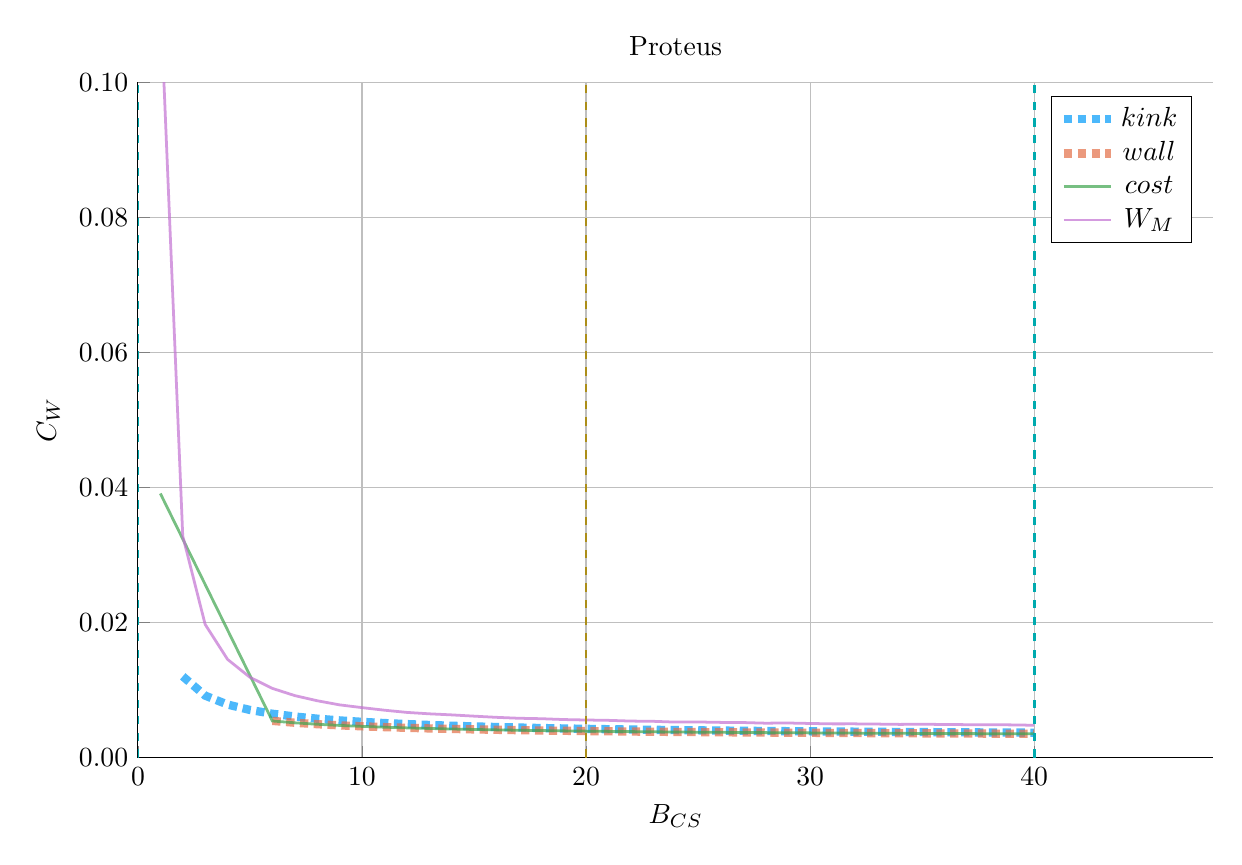
\begin{tikzpicture}[]
\begin{axis}[height = {101.6mm}, ylabel = {${C}_{W}$}, title = {Proteus}, xmin = {0.0}, xmax = {48.0}, ymax = {0.1}, xlabel = {${B}_{CS}$}, {unbounded coords=jump, scaled x ticks = false, xticklabel style={rotate = 0}, xmajorgrids = true, xtick = {0.0,10.0,20.0,30.0,40.0}, xticklabels = {0,10,20,30,40}, xtick align = inside, axis lines* = left, scaled y ticks = false, yticklabel style={rotate = 0}, ymajorgrids = true, ytick = {0.0,0.02,0.04,0.06,0.08,0.1}, yticklabels = {0.00,0.02,0.04,0.06,0.08,0.10}, ytick align = inside, axis lines* = left,     xshift = 0.0mm,
    yshift = 0.0mm,
    axis background/.style={fill={rgb,1:red,1.00000000;green,1.00000000;blue,1.00000000}}
, colorbar style={title=}}, ymin = {0.0}, width = {152.4mm}]\addplot+ [color = {rgb,1:red,0.00000000;green,0.60560316;blue,0.97868012},
draw opacity=0.7,
line width=3,
dotted,mark = none,
mark size = 2.0,
mark options = {
    color = {rgb,1:red,0.00000000;green,0.00000000;blue,0.00000000}, draw opacity = 0.7,
    fill = {rgb,1:red,0.00000000;green,0.60560316;blue,0.97868012}, fill opacity = 0.7,
    line width = 1,
    rotate = 0,
    solid
}]coordinates {
(2.0, 0.01203588028473762)
(3.0, 0.009184398565447248)
(4.0, 0.007862884013421416)
(5.0, 0.007057989599185806)
(6.0, 0.006502613319842857)
(7.0, 0.006090672614199328)
(8.0, 0.005770350019203115)
(9.0, 0.005512859892710094)
(10.0, 0.005300727695239639)
(11.0, 0.005122630604633569)
(12.0, 0.004970854616305319)
(13.0, 0.00483993073972795)
(14.0, 0.0047258536533321)
(15.0, 0.004625609812173743)
(16.0, 0.004536878856245803)
(17.0, 0.004457840030041975)
(18.0, 0.004387039347241793)
(19.0, 0.004323297793305687)
(20.0, 0.004265648725148842)
(21.0, 0.00421328852908289)
(22.0, 0.004165543387382086)
(23.0, 0.0041218418382133306)
(24.0, 0.004081697424729452)
(25.0, 0.004044691025187507)
(26.0, 0.004010460170934446)
(27.0, 0.00397868942182741)
(28.0, 0.003949102890414613)
(29.0, 0.003921458228696752)
(30.0, 0.0038955417483358588)
(31.0, 0.00387116442730114)
(32.0, 0.003848158715413871)
(33.0, 0.0038263753834889853)
(34.0, 0.003805681791784416)
(35.0, 0.0037859598267780737)
(36.0, 0.003767103936991627)
(37.0, 0.003749019788626583)
(38.0, 0.0037316235037579658)
(39.0, 0.0037148400629903496)
(40.0, 0.003698602652227772)
};
\addlegendentry{$kink$}
\addplot+ [color = {rgb,1:red,0.88887350;green,0.43564919;blue,0.27812294},
draw opacity=0.7,
line width=3,
dotted,mark = none,
mark size = 2.0,
mark options = {
    color = {rgb,1:red,0.00000000;green,0.00000000;blue,0.00000000}, draw opacity = 0.7,
    fill = {rgb,1:red,0.88887350;green,0.43564919;blue,0.27812294}, fill opacity = 0.7,
    line width = 1,
    rotate = 0,
    solid
}]coordinates {
(6.0, 0.0054444534313977866)
(7.0, 0.005168634641274746)
(8.0, 0.004954271193511655)
(9.0, 0.004781774855931542)
(10.0, 0.0046393940524333595)
(11.0, 0.004519572327657892)
(12.0, 0.004417187891782309)
(13.0, 0.004328621916738755)
(14.0, 0.004251229863078844)
(15.0, 0.004183024392188461)
(16.0, 0.004122476375660697)
(17.0, 0.004068385219748399)
(18.0, 0.004019791621043741)
(19.0, 0.003975917241919141)
(20.0, 0.003936121998618529)
(21.0, 0.0038998731854890116)
(22.0, 0.0038667227426346573)
(23.0, 0.0038362902440819057)
(24.0, 0.003808249979473852)
(25.0, 0.003782321013899768)
(26.0, 0.003758259446775421)
(27.0, 0.003735852316365348)
(28.0, 0.0037149127505960292)
(29.0, 0.0036952760721994664)
(30.0, 0.003676796641638663)
(31.0, 0.003659345275564596)
(32.0, 0.003642807117806076)
(33.0, 0.0036270798687725717)
(34.0, 0.003612072300608303)
(35.0, 0.0035977030015636596)
(36.0, 0.0035838993052924165)
(37.0, 0.003570596370170802)
(38.0, 0.0035577363809944163)
(39.0, 0.003545267851071995)
(40.0, 0.003533145007184075)
};
\addlegendentry{$wall$}
\addplot+ [color = {rgb,1:red,0.24222430;green,0.64327509;blue,0.30444865},
draw opacity=0.7,
line width=1,
solid,mark = none,
mark size = 2.0,
mark options = {
    color = {rgb,1:red,0.00000000;green,0.00000000;blue,0.00000000}, draw opacity = 0.7,
    fill = {rgb,1:red,0.24222430;green,0.64327509;blue,0.30444865}, fill opacity = 0.7,
    line width = 1,
    rotate = 0,
    solid
}]coordinates {
(1.0, 0.03911143879274214)
(6.0, 0.005431918985170686)
(7.0, 0.005156651927896806)
(8.0, 0.0049427222925668)
(9.0, 0.004770577307210836)
(10.0, 0.004628487505103093)
(11.0, 0.004508911021409933)
(12.0, 0.004406736153465557)
(13.0, 0.004318351239259131)
(14.0, 0.0042411171388798095)
(15.0, 0.004173050519899446)
(16.0, 0.00411262543808849)
(17.0, 0.0040586437812760905)
(18.0, 0.004010148222137883)
(19.0, 0.003966362101140297)
(20.0, 0.003926646631736614)
(21.0, 0.003890470261769361)
(22.0, 0.003857385855340664)
(23.0, 0.003827013846123357)
(24.0, 0.003799029152446192)
(25.0, 0.0037731515135378028)
(26.0, 0.0037491374742800476)
(27.0, 0.003726774572373303)
(28.0, 0.0037058763309042774)
(29.0, 0.0036862784148944654)
(30.0, 0.0036678355176402353)
(31.0, 0.0036504187072176437)
(32.0, 0.0036339133609214515)
(33.0, 0.003618217419267161)
(34.0, 0.003603239855200063)
(35.0, 0.0035888993956205303)
(36.0, 0.003575123536625824)
(37.0, 0.0035618476053302967)
(38.0, 0.00354901385682175)
(39.0, 0.0035365709088021192)
(40.0, 0.0035244731223137145)
};
\addlegendentry{$cost$}
\addplot+ [color = {rgb,1:red,0.76444018;green,0.44411178;blue,0.82429754},
draw opacity=0.7,
line width=1,
solid,mark = none,
mark size = 2.0,
mark options = {
    color = {rgb,1:red,0.00000000;green,0.00000000;blue,0.00000000}, draw opacity = 0.7,
    fill = {rgb,1:red,0.76444018;green,0.44411178;blue,0.82429754}, fill opacity = 0.7,
    line width = 1,
    rotate = 0,
    solid
}]coordinates {
(1.0, 0.11281791824873516)
(2.0, 0.032817502153924004)
(3.0, 0.019728226993225767)
(4.0, 0.014550673387607675)
(5.0, 0.01189537503222638)
(6.0, 0.010254586386818185)
(7.0, 0.009187722848027494)
(8.0, 0.008426409595366063)
(9.0, 0.007814460956383539)
(10.0, 0.007407116893402244)
(11.0, 0.007026609234473925)
(12.0, 0.006699623094822548)
(13.0, 0.006490049586328449)
(14.0, 0.006332285776340749)
(15.0, 0.006145121123500574)
(16.0, 0.005968637732544897)
(17.0, 0.005831116183284295)
(18.0, 0.005766436928694199)
(19.0, 0.005641758652539625)
(20.0, 0.005573536740322697)
(21.0, 0.005522757977005573)
(22.0, 0.005416005772196298)
(23.0, 0.005379655600977924)
(24.0, 0.005261536268439173)
(25.0, 0.005281022329992938)
(26.0, 0.0052218684208626695)
(27.0, 0.005199327855049588)
(28.0, 0.005104248642193906)
(29.0, 0.005130959429711627)
(30.0, 0.005061392939220031)
(31.0, 0.005001395595923804)
(32.0, 0.005003038146366862)
(33.0, 0.004969709625977857)
(34.0, 0.004924506782614121)
(35.0, 0.004946663939864212)
(36.0, 0.004912455965902953)
(37.0, 0.004883749116586274)
(38.0, 0.004871307710986148)
(39.0, 0.004851151446945242)
(40.0, 0.004795575554984452)
};
\addlegendentry{$W_M$}
\addplot+ [color = {rgb,1:red,0.67554396;green,0.55566233;blue,0.09423434},
draw opacity=1.0,
line width=1,
dashed,mark = none,
mark size = 2.0,
mark options = {
    color = {rgb,1:red,0.00000000;green,0.00000000;blue,0.00000000}, draw opacity = 1.0,
    fill = {rgb,1:red,0.67554396;green,0.55566233;blue,0.09423434}, fill opacity = 1.0,
    line width = 1,
    rotate = 0,
    solid
},forget plot]coordinates {
(20.0, 0.0)
(20.0, 0.1)
};
\addplot+ [color = {rgb,1:red,0.00000048;green,0.66575898;blue,0.68099695},
draw opacity=1.0,
line width=1,
dashed,mark = none,
mark size = 2.0,
mark options = {
    color = {rgb,1:red,0.00000000;green,0.00000000;blue,0.00000000}, draw opacity = 1.0,
    fill = {rgb,1:red,0.00000048;green,0.66575898;blue,0.68099695}, fill opacity = 1.0,
    line width = 1,
    rotate = 0,
    solid
},forget plot]coordinates {
(0.0, 0.0)
(0.0, 0.1)
};
\addplot+ [color = {rgb,1:red,0.00000048;green,0.66575898;blue,0.68099695},
draw opacity=1.0,
line width=1,
dashed,mark = none,
mark size = 2.0,
mark options = {
    color = {rgb,1:red,0.00000000;green,0.00000000;blue,0.00000000}, draw opacity = 1.0,
    fill = {rgb,1:red,0.00000048;green,0.66575898;blue,0.68099695}, fill opacity = 1.0,
    line width = 1,
    rotate = 0,
    solid
},forget plot]coordinates {
(40.0, 0.0)
(40.0, 0.1)
};
\end{axis}

\end{tikzpicture}

    \end{adjustbox}
        \caption{Solenoid Strength Sensitivity}
    \end{subfigure}
    \hfill
    \begin{subfigure}[t]{0.48\textwidth}
        \centering
    \begin{adjustbox}{width=\textwidth}
      \Large
      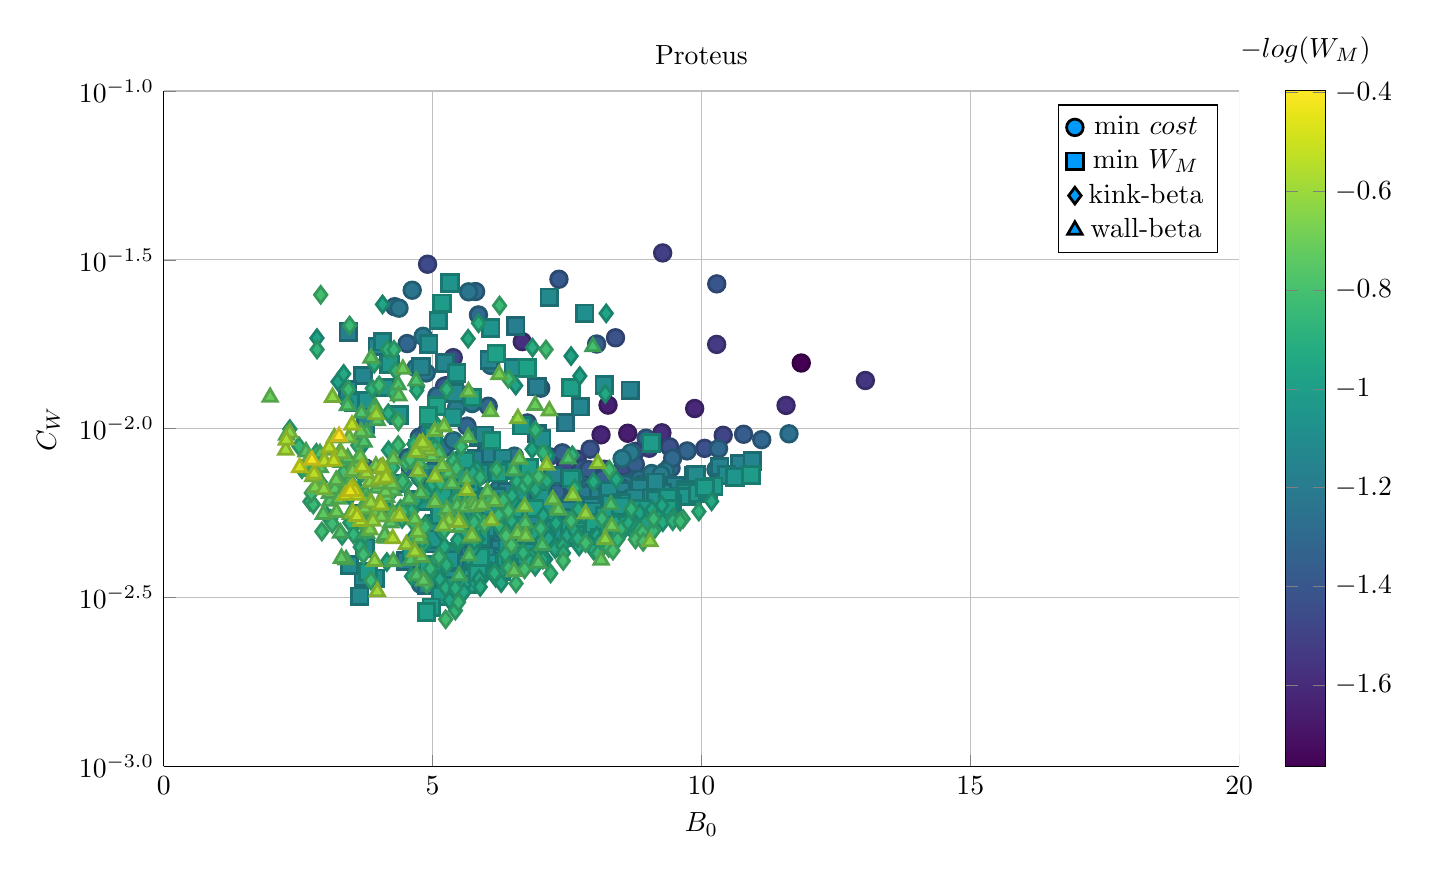
\begin{tikzpicture}[]
\begin{axis}[colorbar = {true}, height = {101.6mm}, ylabel = {${C}_{W}$}, title = {Proteus}, xmin = {0.0}, xmax = {20.0}, ymax = {0.1}, ymode = {log}, xlabel = {${B}_{0}$}, {unbounded coords=jump, scaled x ticks = false, xticklabel style={rotate = 0}, xmajorgrids = true, xtick = {0.0,5.0,10.0,15.0,20.0}, xticklabels = {0,5,10,15,20}, xtick align = inside, axis lines* = left, scaled y ticks = false, yticklabel style={rotate = 0}, log basis y=10, ymajorgrids = true, ytick = {0.001,0.0031622776601683794,0.01,0.03162277660168379,0.1}, yticklabels = {$10^{-3.0}$,$10^{-2.5}$,$10^{-2.0}$,$10^{-1.5}$,$10^{-1.0}$}, ytick align = inside, axis lines* = left,     xshift = 0.0mm,
    yshift = 0.0mm,
    axis background/.style={fill={rgb,1:red,1.00000000;green,1.00000000;blue,1.00000000}}
, colormap={plots}{rgb=(0.26700400,0.00487400,0.32941500), rgb=(0.27794100,0.05632400,0.38119100), rgb=(0.28291000,0.10539300,0.42690200), rgb=(0.28229000,0.14591200,0.46151000), rgb=(0.27619400,0.19007400,0.49300100), rgb=(0.26514500,0.23295600,0.51659900), rgb=(0.25042500,0.27429000,0.53310300), rgb=(0.23360300,0.31382800,0.54391400), rgb=(0.21813000,0.34743200,0.55003800), rgb=(0.20123900,0.38367000,0.55429400), rgb=(0.18555600,0.41857000,0.55675300), rgb=(0.17117600,0.45253000,0.55796500), rgb=(0.15772900,0.48593200,0.55801300), rgb=(0.14618000,0.51541300,0.55682300), rgb=(0.13374300,0.54853500,0.55354100), rgb=(0.12346300,0.58168700,0.54744500), rgb=(0.11948300,0.61481700,0.53769200), rgb=(0.12632600,0.64410700,0.52531100), rgb=(0.15014800,0.67663100,0.50658900), rgb=(0.19109000,0.70836600,0.48228400), rgb=(0.24607000,0.73891000,0.45202400), rgb=(0.31192500,0.76782200,0.41558600), rgb=(0.37777900,0.79178100,0.37793900), rgb=(0.45867400,0.81636300,0.32972700), rgb=(0.54552400,0.83803900,0.27562600), rgb=(0.63690200,0.85654200,0.21662000), rgb=(0.73088900,0.87191600,0.15602900), rgb=(0.81457600,0.88339300,0.11034700), rgb=(0.90631100,0.89485500,0.09812500), rgb=(0.99324800,0.90615700,0.14393600)}, colorbar style={title=$-log( W_M )$}}, ymin = {0.001}, width = {152.4mm}]\addplot+[scatter, scatter src=explicit, only marks = {true}, color = {rgb,1:red,0.00000000;green,0.60560316;blue,0.97868012},
draw opacity=1,
line width=0,
solid,mark = *,
mark size = 3.0,
mark options = {
    color = {rgb,1:red,0.00000000;green,0.00000000;blue,0.00000000}, draw opacity = 1.0,
    fill = {rgb,1:red,0.00000000;green,0.60560316;blue,0.97868012}, fill opacity = 1,
    line width = 1,
    rotate = 0,
    solid
}] coordinates {
(11.855851167264671, 0.015650867313707448) [-1.7651507846396934]
(8.62894306410229, 0.009694646552347688) [-1.652530796858066]
(8.262669569295957, 0.011744038729478485) [-1.647000146345283]
(8.132345586482765, 0.009590177278586947) [-1.6184546481250472]
(9.87352129314419, 0.011474300333025303) [-1.6124908438767973]
(9.26466071494926, 0.00972401084478665) [-1.5828949402967583]
(6.667811597046653, 0.018106858351787505) [-1.577618500437912]
(11.573395463568893, 0.011719738653164523) [-1.56873554690934]
(5.264528343635174, 0.013419897432724169) [-1.5599002750009094]
(13.048135395345042, 0.013892471464509717) [-1.5518482038436605]
(10.282796584070674, 0.017767343192357253) [-1.5302287668791192]
(9.278542294221232, 0.033146306422516245) [-1.5115301730224102]
(7.5044360623009565, 0.007510212646674021) [-1.5013825191439996]
(9.02784009554164, 0.008751202105526691) [-1.4958902811815062]
(8.710683108208965, 0.00816949735167802) [-1.4892617900728689]
(7.687377168804008, 0.008118078139228204) [-1.4884348201277007]
(10.404534949568816, 0.009559158760396884) [-1.4866425610729714]
(5.384524713145202, 0.01623184139531336) [-1.4835478223239928]
(7.472857057569771, 0.007837831837729894) [-1.4780728724015184]
(4.906484287411937, 0.03069401611625924) [-1.4650031348255397]
(7.111580297007043, 0.006765803188842749) [-1.4601242927308113]
(8.773685022223647, 0.008568870415676909) [-1.453691298071198]
(8.545510256202396, 0.007723927816166263) [-1.4489094778079963]
(7.070436548811644, 0.006162431971740805) [-1.432973868001932]
(6.884154096232421, 0.006329451983138475) [-1.4325147285303634]
(9.405921329983288, 0.008839617844718544) [-1.4268866569895065]
(10.057985274469397, 0.008744700190770928) [-1.4268347679685771]
(8.401821549997786, 0.018590297650719324) [-1.4237681445033143]
(8.189937032371649, 0.007587250291191641) [-1.4234658725845162]
(8.234578254729767, 0.007390656211515189) [-1.4109108269606008]
(7.92991212471289, 0.008694085637837138) [-1.4079262096010774]
(6.59839258184741, 0.00634066157530613) [-1.407330123320285]
(10.284931156770094, 0.026840973164111593) [-1.3996791570309395]
(7.3137838143058795, 0.007040053838733538) [-1.3974870797438]
(5.221820332167986, 0.013359280479800206) [-1.3946269662443698]
(7.785957307166937, 0.007634837530984513) [-1.3905305073664083]
(7.069469201177765, 0.006488653571629467) [-1.3895960301339119]
(6.200523563918331, 0.00554611680879456) [-1.381931002288656]
(7.340133149046422, 0.00695131625200887) [-1.3818272949203658]
(7.349866215424601, 0.027704627448181397) [-1.3812563757949996]
(7.351199097200025, 0.00681167564679013) [-1.379699079550137]
(8.120289345307025, 0.006715817539753603) [-1.376650573885692]
(7.90274300232169, 0.00757067906104037) [-1.3758581110553065]
(7.565484576443418, 0.006499559071472007) [-1.375220700855124]
(7.688718501611012, 0.00646934556613389) [-1.3742348635950123]
(7.005633077388933, 0.0063267927368600325) [-1.3713423550361032]
(7.166534585210968, 0.008267480512087599) [-1.370057699317172]
(5.695615872659735, 0.004988896324536347) [-1.3686239973313072]
(6.620180775083285, 0.005540386026064644) [-1.3680076928767484]
(5.712356159098289, 0.005024205798518008) [-1.3672266212882762]
(10.783439028923059, 0.009628839399324697) [-1.3667105305870977]
(6.000471468140266, 0.0050592629231849704) [-1.3651176317240314]
(8.050752136473724, 0.017814080806893125) [-1.3612722200713383]
(8.77043990632116, 0.007840171434328094) [-1.360737823431438]
(7.010340303297389, 0.013182987051350502) [-1.3596008789905631]
(7.295294539644262, 0.006730765435871485) [-1.3568098625263256]
(6.641599582701438, 0.005632641769207446) [-1.3562925407270994]
(6.645748730966029, 0.005613911931897123) [-1.3540300242042478]
(6.054699810485283, 0.005176189759381431) [-1.3527684291391184]
(9.401252816575663, 0.007678792615766904) [-1.3513432280511455]
(5.581708167132495, 0.006888425944911811) [-1.3508742741062625]
(7.803535098905909, 0.006674090356682625) [-1.348444904526092]
(6.76411548346407, 0.010402669872398145) [-1.3482429808137002]
(8.969455503638764, 0.009376571407375644) [-1.3481015746033576]
(5.634510628688515, 0.012583797530216616) [-1.34746159692277]
(8.156032796881272, 0.007115527316776566) [-1.3450418873098828]
(7.056939291922313, 0.006464286011476574) [-1.3449397649071608]
(7.240799475525162, 0.006186516144095541) [-1.344834769873685]
(6.571134452649435, 0.0053864817732829605) [-1.3436955024234147]
(7.4120702527384665, 0.00848434463520388) [-1.3426163725681677]
(5.934011898969639, 0.004938310227983135) [-1.3374912582230194]
(7.37766442956072, 0.006636608478826529) [-1.335539302100867]
(5.026669706190863, 0.007606581585076429) [-1.3352915983538123]
(6.825792187162438, 0.006029019944814239) [-1.331337874103357]
(9.732916904654346, 0.008594819258321628) [-1.3310780697195672]
(5.698038434377145, 0.004728216221281147) [-1.3292068036291638]
(6.854283769326888, 0.005953363383436291) [-1.32828646244698]
(4.7527705925878685, 0.009441137210103956) [-1.3280975618898123]
(6.452485475407575, 0.005079524630506098) [-1.3278697867431468]
(6.6282734062471, 0.005749625528658903) [-1.327757292865828]
(7.362442088263758, 0.006249734903697681) [-1.3253106415861637]
(6.357926345811093, 0.005155209960292018) [-1.3237407060184172]
(9.434691757978365, 0.007650804529712704) [-1.3217246458754282]
(5.945683748997239, 0.004926318213851794) [-1.319376268743699]
(5.716699212704698, 0.004774448071559269) [-1.3182101821558738]
(7.9999703999657505, 0.0066268624262571275) [-1.31770129332637]
(4.526018058829261, 0.017867829271260238) [-1.3171626271127284]
(7.307142270921693, 0.006479743346210051) [-1.3144438328362922]
(5.64022055353738, 0.010177994071422254) [-1.314397397461996]
(11.121291715489328, 0.009279261565995508) [-1.3134452963620502]
(6.890660641840135, 0.005896178522672516) [-1.3126768401499638]
(5.8496112618323926, 0.007223214696135702) [-1.3123916957087167]
(3.755618871416242, 0.007643344629724278) [-1.3117090270675453]
(6.965828665871357, 0.0062843154751196315) [-1.3112976001573549]
(7.132942553696917, 0.006316305209750007) [-1.3102933400586538]
(6.034623082086722, 0.011655743235665423) [-1.3084666426112759]
(9.464190150712176, 0.008181643780093392) [-1.3081739820914746]
(6.735484315816856, 0.005920113041607297) [-1.3081169022767745]
(6.329532230716051, 0.005266304291939928) [-1.3075986397555424]
(6.949512174456946, 0.0056632699287416785) [-1.3038897119548887]
(5.7123865302563095, 0.004515583648974614) [-1.3034916079905217]
(4.588431546307119, 0.00762405310841983) [-1.301506470226052]
(5.8529754306366, 0.021723513711501174) [-1.2978787946122285]
(6.763583440942078, 0.005860560202229156) [-1.297460949292816]
(5.79974352272628, 0.02547444831481485) [-1.2953226778576867]
(4.294506467374343, 0.022974551007964673) [-1.2951062787178942]
(10.317711969577175, 0.008727794605170999) [-1.2946978796261759]
(7.030442720189729, 0.00606442154900928) [-1.293243062455323]
(6.3155245633398005, 0.00478216163852665) [-1.2916316854649297]
(5.594153930448576, 0.004505685536187866) [-1.291573412415986]
(7.0608047385200905, 0.006201757851874389) [-1.2910367642815292]
(8.746159160738731, 0.007056272547770033) [-1.2894268757747884]
(5.790961836119614, 0.004812007322004063) [-1.2891780169645117]
(7.13931972393237, 0.005900795309436559) [-1.2883016772579983]
(5.642350264315365, 0.004575860387174974) [-1.2877120777365891]
(5.500511487756749, 0.007501625869556503) [-1.2825608117529994]
(5.1870060839860015, 0.004048206616482656) [-1.2803416949249293]
(5.0793762257146975, 0.012501014524680899) [-1.2790944723531177]
(4.900710067477188, 0.009849033693022476) [-1.2789599032268324]
(5.416336002756713, 0.004266328381972482) [-1.278637308935949]
(7.047880217226236, 0.00602317781329061) [-1.2752962713941192]
(4.537987048593646, 0.008202673797589401) [-1.2724318730764337]
(6.7947527911354095, 0.005313590913225172) [-1.26778944603233]
(7.547856502776895, 0.005746237915345085) [-1.2652894696394015]
(8.337373800803634, 0.0063394092295352205) [-1.263844406219344]
(5.839234828237175, 0.004670640784960837) [-1.2622412045786418]
(6.307588148065544, 0.005025369604276285) [-1.2622057750392766]
(6.369182324037021, 0.004715175023029078) [-1.2568407944078956]
(7.25221896281004, 0.005515822538041083) [-1.2564369672634057]
(5.207422458409709, 0.008763742702873716) [-1.255580803936347]
(8.846964102011665, 0.007090160917314494) [-1.2542825781236586]
(11.62801313878366, 0.009658252430988482) [-1.253606675738751]
(6.586437041421525, 0.005078101074449218) [-1.2533258835374417]
(5.896819232149536, 0.004668333949768413) [-1.252740293490489]
(7.218625057420257, 0.005623439530060779) [-1.2512906609771755]
(4.770007649977626, 0.007192663750971734) [-1.2505906665339703]
(6.391248250395476, 0.004753912504004936) [-1.2505667349102745]
(6.722228809625436, 0.00547669175115548) [-1.2505409706978425]
(5.9975644347104575, 0.008585550973626429) [-1.2504311283223648]
(6.220483255591395, 0.00536142422310656) [-1.2495193060816674]
(7.131398255569569, 0.005891517799670805) [-1.2472203996667584]
(4.620896334693883, 0.025703839631456088) [-1.246340221801285]
(5.634708074324937, 0.004426672964739238) [-1.246337044553182]
(6.0053836269885, 0.004733745531528537) [-1.2444533586241864]
(6.122472771064873, 0.004373459187272198) [-1.2410504069560844]
(4.881468969197191, 0.014622918962551527) [-1.2404616678069278]
(5.669873863181108, 0.025422666134658947) [-1.2402101811954278]
(9.159921449108527, 0.00699405114862055) [-1.2399625556579728]
(6.619988989498716, 0.005459593535350185) [-1.2395775558220574]
(4.0721743569002395, 0.006780135026174841) [-1.238968027160994]
(8.487125648729805, 0.006381273355008305) [-1.2381935518916032]
(5.785136288326493, 0.005454977773134567) [-1.2372164242860222]
(7.805870043590986, 0.006162937475975255) [-1.2359322527835273]
(6.521775930847536, 0.008295248979234676) [-1.2345953253761524]
(7.299795216034374, 0.005661235915534237) [-1.2333782101635051]
(6.654376116038794, 0.005116145429327062) [-1.2329256482335589]
(8.586321868785943, 0.0068738253515159406) [-1.2318041138227]
(5.871716076416853, 0.007759607253139788) [-1.2286780396839752]
(5.525881431830733, 0.004270512991179436) [-1.225800447150557]
(4.37566370657649, 0.022744869820021597) [-1.2237626122718148]
(5.386416012885563, 0.009221148903357415) [-1.2192315569877235]
(5.735606858683557, 0.011868028475244749) [-1.2191811590789894]
(8.68706974133124, 0.008481483201532794) [-1.2185680785343938]
(8.63032181590475, 0.00622802822970762) [-1.2179132583990178]
(8.508158073563377, 0.006703260233628488) [-1.2171472173843672]
(7.953691408978824, 0.00633213628058925) [-1.2167448502658762]
(6.081331959057098, 0.015392818825938645) [-1.2162995250149307]
(5.225401290559421, 0.003872910530196867) [-1.215703789534109]
(5.988978974443945, 0.004720977485089404) [-1.2156312790675603]
(9.073087462786646, 0.00736963569440644) [-1.2145283350978044]
(7.217725198328268, 0.005383150867826381) [-1.214317974252912]
(5.536577745729214, 0.004178935326843822) [-1.2138536176262873]
(4.776559777248383, 0.0034641548226198885) [-1.2119360055173332]
(5.211688187540344, 0.0038140534914709043) [-1.2104347246988538]
(10.269380266980404, 0.007570292211977012) [-1.2084631186053005]
(6.918845939903695, 0.0052385995930077645) [-1.2083264519217767]
(7.0692693982238906, 0.005083028024589718) [-1.2073346872626274]
(5.874112036399968, 0.004039129704078142) [-1.2071975929322125]
(4.690082401892927, 0.01513911751066285) [-1.2067840670536927]
(7.861161945792819, 0.006395373245847939) [-1.206736577191552]
(9.326423266814658, 0.007483645463069493) [-1.2065799786199445]
(8.029413669351802, 0.005698374888186277) [-1.203843641047789]
(6.959732144718079, 0.005550896360654382) [-1.203724365314369]
(6.960477287319412, 0.005010777712400389) [-1.2024406864855146]
(7.654476699386534, 0.007157947201399507) [-1.2021169810907544]
(4.823547237227045, 0.01877759730610099) [-1.2015933815507112]
(6.062862639710857, 0.004489267037355289) [-1.2014423796656961]
(8.999102001729389, 0.006374667856956503) [-1.2011965112492808]
(7.2717504340335415, 0.00572395742880883) [-1.2005427289121806]
(6.227413325881237, 0.0066192080125215165) [-1.1994215784439877]
(9.247503176233229, 0.007316062816603203) [-1.1975084180232178]
(5.443249511926066, 0.011502671870448664) [-1.1972619972446426]
(6.742357647461489, 0.005266662336518346) [-1.1967371969067386]
(5.926964832086266, 0.004368135902166705) [-1.1965134818457024]
(8.524769827029726, 0.008154332104698897) [-1.196084536648355]
(8.867575034400405, 0.006843978332329513) [-1.1943424204563022]
(6.457339766119646, 0.005029914775543452) [-1.1908054127888088]
};
\addlegendentry{min $cost$}
\addlegendentry{min $W_M$}
\addlegendentry{kink-beta}
\addlegendentry{wall-beta}
\addplot+[scatter, scatter src=explicit, only marks = {true}, color = {rgb,1:red,0.00000000;green,0.60560316;blue,0.97868012},
draw opacity=1,
line width=0,
solid,mark = square*,
mark size = 3.0,
mark options = {
    color = {rgb,1:red,0.00000000;green,0.00000000;blue,0.00000000}, draw opacity = 1.0,
    fill = {rgb,1:red,0.00000000;green,0.60560316;blue,0.97868012}, fill opacity = 1,
    line width = 1,
    rotate = 0,
    solid
}] coordinates {
(7.4724590738720655, 0.010422279639263054) [-1.1890033537880158]
(6.938996985119089, 0.009658294464102987) [-1.1883675827161198]
(6.9393893920794385, 0.013313745665171912) [-1.1879538738656286]
(6.377850385556073, 0.006487414571263668) [-1.1878029685724296]
(6.547487324963764, 0.020145877705477357) [-1.186260879134981]
(8.029613686159495, 0.005801884747670386) [-1.1859242026174677]
(5.6874025972941205, 0.004217349677698315) [-1.183889066210908]
(7.827309596895398, 0.0058827996938258294) [-1.1830291222504283]
(5.8219713598117036, 0.008160599297710009) [-1.1826268505607591]
(6.946718058585209, 0.004857174007518612) [-1.182365307189366]
(3.434094114791118, 0.01935279381255584) [-1.1822251925764147]
(6.23809783755075, 0.00447855648592392) [-1.1813612663460882]
(5.88781791976068, 0.00428725320402622) [-1.1785285195809967]
(4.505121226933233, 0.004053651772674214) [-1.1775655951090325]
(6.553162158329651, 0.005121496915389368) [-1.17705398157876]
(5.8303432949169745, 0.005890819973806921) [-1.1767452937515073]
(8.807822926389145, 0.006104718148251412) [-1.1766083315756861]
(4.18691738643155, 0.01556268699280997) [-1.173888237216638]
(7.55203601905607, 0.005882961839613334) [-1.1734465174435744]
(5.819836385827624, 0.005961179911412564) [-1.1729466514857931]
(9.116693027577789, 0.006287276174883399) [-1.172839252676928]
(3.659189590525744, 0.005599267038542826) [-1.1727769211527406]
(7.004035835152084, 0.005070632392189801) [-1.1727372361954858]
(4.897086463141796, 0.003434292526080427) [-1.1726542785062386]
(8.087708955601924, 0.0062657093568900535) [-1.1703764252048678]
(6.7024429891400565, 0.004942047034638912) [-1.1699166462753263]
(5.893015258208656, 0.004183590560340062) [-1.1681831393061217]
(7.479710666339309, 0.005170881199231806) [-1.1671080842733117]
(9.508375514310952, 0.006777996547666784) [-1.1655606692177785]
(6.075560203652315, 0.008402469668507205) [-1.165303541813206]
(6.61932998550545, 0.004666935296152095) [-1.1643973078802388]
(6.286558265163782, 0.004663766235492665) [-1.1632535008384055]
(5.050068824721165, 0.004566940606242733) [-1.1631989573193973]
(7.688714523679582, 0.0054331000812183365) [-1.1630392685982025]
(8.505800422917172, 0.006544368204474158) [-1.1625753891662707]
(8.975209897762664, 0.006511116933487475) [-1.1617936783337066]
(8.380983437312786, 0.006126048639979384) [-1.159367616011031]
(8.67470730810651, 0.012995381528200805) [-1.1593260324319568]
(5.960621269295445, 0.004013416769217783) [-1.1592024857112633]
(6.282535161243701, 0.004530529794416821) [-1.1590403977294572]
(10.712436821713085, 0.007867971330715704) [-1.1589428109110296]
(7.099415207654768, 0.005330271588661515) [-1.158451320077056]
(10.3395352744249, 0.007724720119696045) [-1.157468772898154]
(6.536306152444655, 0.004436262085616985) [-1.1570637161067505]
(9.855000808062698, 0.007249642226094706) [-1.1563966451418943]
(5.856384724795581, 0.009420901412013665) [-1.1561531921827275]
(7.454679880823048, 0.0057898611640113395) [-1.1538328200442942]
(5.14753239685863, 0.007237376261288284) [-1.1525173430901554]
(6.856563325018079, 0.004881019954742076) [-1.1522162283529644]
(7.618840457764884, 0.0059379940430840635) [-1.151968932860403]
(8.398440991699191, 0.0061407721476487214) [-1.1511586507355254]
(4.781165601129724, 0.015255960449664327) [-1.1509834966159156]
(6.247011281135245, 0.004419080970160178) [-1.1503660387736743]
(3.7553680100049234, 0.01032617135589161) [-1.1500086948877408]
(5.5152996897670015, 0.004014883666259908) [-1.1494080253790357]
(7.800728278542519, 0.005291422749753008) [-1.1493093072503229]
(6.054088477025007, 0.01598351560152435) [-1.1489823622220707]
(5.411295562966824, 0.003915099463846501) [-1.1484511044037433]
(7.052045109627868, 0.005020529922825154) [-1.1483999797493492]
(5.28488049549897, 0.0034947010100993764) [-1.147064765638366]
(7.62011089503286, 0.005859550653426385) [-1.1465028274549764]
(7.468210164743146, 0.005641165149475234) [-1.144883586902141]
(5.595946792423691, 0.007176119328254024) [-1.144368544047569]
(10.943656185786155, 0.00802165691682325) [-1.1435280806157744]
(7.908061023064291, 0.005447269817044685) [-1.1433393449411435]
(8.854582349908517, 0.006668732693209443) [-1.143332108158641]
(6.549837080949351, 0.004886014774808058) [-1.143184585873657]
(3.9729755898485215, 0.017515494611674454) [-1.1428249654095861]
(3.703954177548893, 0.014377117697389604) [-1.1427984862828113]
(3.4213090828497417, 0.013005276311642224) [-1.142397010267489]
(6.02709699747974, 0.005929095379259443) [-1.1423708774410877]
(5.231750077921478, 0.01565086593371781) [-1.1422424769576425]
(7.2349136535832095, 0.007266091038483963) [-1.140012696356206]
(7.647205004097057, 0.005840600330748377) [-1.1399465227440013]
(6.532016233135844, 0.00480284773560221) [-1.1387943392990294]
(7.523885505796154, 0.005752426766742318) [-1.1382802201938975]
(7.750130276532692, 0.011612930840038163) [-1.1380314198362265]
(9.276469763067444, 0.006446360072583165) [-1.137892443914052]
(5.952941013085345, 0.009562541252399106) [-1.1311113631375915]
(7.951426521304668, 0.005743536904522906) [-1.1302954325651586]
(5.952653119927932, 0.0041760314888273755) [-1.1295543261638465]
(8.253192497448524, 0.006161648966500728) [-1.129462828049983]
(5.512192429439468, 0.00369116854025651) [-1.1277963061708562]
(6.180741676638315, 0.006278926396423389) [-1.126807171194116]
(6.608627477861355, 0.004487529275565533) [-1.1267021554022474]
(9.14457555501132, 0.006938744439971839) [-1.1265761162904897]
(5.310301950330671, 0.004304336836767321) [-1.1261385034152473]
(7.969320198807478, 0.005917258047258142) [-1.1260458936236624]
(7.954215183655014, 0.005885263457738176) [-1.1250537668582923]
(6.771595293849517, 0.005616858230043609) [-1.124511019242948]
(6.641944516873176, 0.004843731890681865) [-1.1236988869720232]
(6.896134858333351, 0.005173923137495115) [-1.1235064786985465]
(3.7132325707792995, 0.003624821435760545) [-1.1232730371267585]
(4.936839162331792, 0.007429853985811719) [-1.1231293548483412]
(6.555316024199809, 0.005231942783984398) [-1.1209978185544383]
(6.304604592673814, 0.008169617815892689) [-1.1196911148335087]
(8.737416781995437, 0.0061580609115664325) [-1.1194748634113345]
(6.123815672401932, 0.004188882178419093) [-1.119418152841014]
(8.324353852438948, 0.005791769416647159) [-1.1191123923650526]
(6.830685941792606, 0.004931972266091366) [-1.1181736482095217]
(8.279157421008941, 0.005611347227289511) [-1.1176702646643628]
(7.172394160745635, 0.024480989089009208) [-1.1175403888423328]
(6.753756430979739, 0.004518885765871233) [-1.1174827013795072]
(8.76524294869496, 0.0062233325455323925) [-1.1174414411464733]
(5.952289891041446, 0.006299808378708293) [-1.1171134960728113]
(6.523754565443294, 0.004568184715721437) [-1.1171111976535804]
(5.4096290381473375, 0.012757776435747556) [-1.1168806186241906]
(9.896916686410892, 0.007305420869085463) [-1.1160945644374545]
(8.286804128590813, 0.005340773800773009) [-1.1139896885893594]
(5.399012890266871, 0.0036233885329560954) [-1.1123768792739945]
(8.296167355721272, 0.005311493039288053) [-1.1112153482766423]
(6.778775360762903, 0.0045000578497955725) [-1.1111283014916062]
(3.642453456441478, 0.003188662256079057) [-1.1108869662710774]
(6.918579935305505, 0.004842654136629077) [-1.1089922492653659]
(6.5071710234613676, 0.00452032863173795) [-1.108391782497311]
(7.258592477367294, 0.00535669926333167) [-1.1082929384878708]
(6.6776055936353265, 0.004745534590751309) [-1.1074346113685616]
(5.3226296796509205, 0.004323464728471098) [-1.1074227437950106]
(10.46985584146923, 0.007293078759243216) [-1.1069130893453907]
(3.4547855533452156, 0.003945456212149148) [-1.106325178133445]
(7.57975455174028, 0.004982808461571556) [-1.1060035644106432]
(5.06842585608741, 0.0052409052861536465) [-1.1038776732161713]
(5.698043204630489, 0.0065314531396132094) [-1.10351060592976]
(7.734654274692709, 0.005173060010686301) [-1.1022315889718237]
(6.228402773452205, 0.005951424789746293) [-1.1016702257969113]
(5.288893434740895, 0.007437806150470808) [-1.100448826904311]
(7.254453932047169, 0.005288339533793414) [-1.0998565094908217]
(6.807046489565401, 0.004337170224988449) [-1.0995498480529582]
(8.496667761878552, 0.005750254423520601) [-1.0992970719713648]
(6.506723144546308, 0.004423364554484401) [-1.0987351440216522]
(8.273277101596172, 0.006535275113176343) [-1.0983869460625248]
(7.024499917691516, 0.006822630998366228) [-1.0977261444257258]
(4.929559505548113, 0.017828562633364364) [-1.0969882385788774]
(6.546519891753608, 0.004407786879742766) [-1.096807077081938]
(6.299458688060015, 0.0041501216036249275) [-1.0962033310727437]
(5.917588131126826, 0.003972749736578854) [-1.0948458082881816]
(6.5027787367036485, 0.015155543307471772) [-1.093965318294314]
(8.191093731826841, 0.013471957430229371) [-1.093275686079877]
(5.765417917352738, 0.003923510470624812) [-1.0931318196649105]
(4.067683728143941, 0.01811006730780237) [-1.0926393639694263]
(5.643295069658257, 0.005671433069083637) [-1.09199330517098]
(5.33448260992027, 0.0035546432563184145) [-1.0916603258728452]
(5.996010919360583, 0.005082501155756355) [-1.091508438458307]
(6.130249778803564, 0.003922207642532424) [-1.0911853630489914]
(5.152309500808404, 0.007129588907950501) [-1.0896526200520398]
(6.613976143688219, 0.004468466025444819) [-1.088663441639713]
(7.828710312153846, 0.021949864805969728) [-1.0877780715734315]
(7.029871400370792, 0.009322832924906896) [-1.0870739196827126]
(6.6598420793586, 0.004672088916974179) [-1.0855818982110972]
(6.33097870945106, 0.004039319528471343) [-1.0844715994400023]
(7.702268833143657, 0.0053439960085053) [-1.0842780595786392]
(6.084754710909704, 0.005760793758021615) [-1.084266572782003]
(7.98999393987453, 0.00569380985136289) [-1.0839928767281124]
(5.068992476376386, 0.0039349920083461085) [-1.0828594792618813]
(9.086048642306793, 0.0062405207423892875) [-1.082853352734588]
(7.44906676523106, 0.0054577800846403015) [-1.0824719035597]
(5.375575122544495, 0.0035809652689903063) [-1.0824709528228211]
(7.386984140765724, 0.005148297391297789) [-1.0814366033908964]
(9.702271536107535, 0.006582162000449632) [-1.0809878234039578]
(9.614854186704672, 0.006301853688415234) [-1.0808972954130593]
(4.645688111866446, 0.006161790226168522) [-1.0797863646031054]
(3.927334262139488, 0.0036086053477567665) [-1.079163153355685]
(6.963971610592974, 0.004793357206410555) [-1.0780309855478056]
(8.244956752748422, 0.0054298508521766365) [-1.076806285491668]
(5.769697532800943, 0.00604411217248383) [-1.0765985094568509]
(7.283344319549832, 0.004828662165485411) [-1.0760641298404754]
(5.392578394594405, 0.005661819547798889) [-1.0757730303287785]
(3.7434225317786316, 0.00443044659495794) [-1.0744056068515366]
(7.7252366425534715, 0.005467468655559742) [-1.073726482715373]
(8.506016241294386, 0.006046667097602973) [-1.072815333291583]
(5.722077224788854, 0.006315687038558954) [-1.0718638391063322]
(3.5290681872248832, 0.011989877345034696) [-1.0710072465261937]
(5.408389828424612, 0.006287200186056995) [-1.0706716976099708]
(5.880603880610476, 0.00739594343637032) [-1.069478881808043]
(3.770984054785403, 0.012080600310741674) [-1.0679830462657767]
(9.144669371614333, 0.006138341400017388) [-1.0670572282884458]
(5.3325423351198395, 0.004085658341340117) [-1.0667391835901658]
(8.316799187366927, 0.006004004929014098) [-1.066302608545655]
(6.389619437625667, 0.004440975162005993) [-1.064104157833971]
(5.324355765249537, 0.026972932068461592) [-1.0640878812065675]
(6.511622532652898, 0.004395996587917252) [-1.0635820925869255]
(6.911249511094287, 0.004423420241739423) [-1.062988318250961]
(7.502962627592097, 0.00480727122317776) [-1.0628036997189863]
(5.469724443246719, 0.0034131330547271113) [-1.062700357913494]
(5.706475165604361, 0.0036974585830479817) [-1.0626514373993834]
(7.276669037534987, 0.004776499853086686) [-1.0610739421064752]
(6.526975357350624, 0.004144297606935685) [-1.0588352037418618]
(5.105089902831069, 0.0209014980088616) [-1.0585986545827941]
(4.374531653432859, 0.010988948677442597) [-1.057135771526312]
(4.122473679442906, 0.013241941603829825) [-1.056315661795303]
(6.078673477412938, 0.019862106250452566) [-1.0562734967702754]
(7.427558910001991, 0.004858658731965693) [-1.0561257856094448]
(7.01015270925273, 0.006223828461257365) [-1.0559814704124602]
(5.014809023336614, 0.004706089102701761) [-1.0555859489072712]
(6.029077134394886, 0.003994614402213268) [-1.0549803415205259]
(9.718000396033032, 0.006463993798881436) [-1.0545713902023608]
(5.896086527792721, 0.0038990516235787613) [-1.054205756099488]
(10.62632239203378, 0.007195479612398366) [-1.0536290024409787]
(9.830251746280974, 0.006286763322784177) [-1.0533216125601341]
(5.653429182632709, 0.004822724612666477) [-1.0529307720930816]
(7.148582094551358, 0.005656264568736301) [-1.0525850668019536]
(9.721783343528084, 0.006295530789348686) [-1.052552508886994]
(6.4747129291886205, 0.007550888758433211) [-1.0509835312174363]
(7.5553171987129115, 0.004904482654727138) [-1.0508250621973283]
(5.689433662550519, 0.006571304536184572) [-1.050680345054969]
(6.819358408267933, 0.004560195418506711) [-1.0506245233592775]
(5.372500908480495, 0.01080264515897382) [-1.0505217359121972]
(9.464104357867244, 0.00597835329976134) [-1.049317623712287]
(9.421645636318559, 0.00605275476812188) [-1.0490747591885061]
(6.83923495211403, 0.004511808104116367) [-1.0489907539423449]
(7.595014509377157, 0.0049153150140211965) [-1.0478434867034416]
(6.9492853284169565, 0.004616652674773231) [-1.0473758850488442]
(6.631954997333512, 0.006447737760929581) [-1.046767629611379]
(4.836574702453568, 0.006114416229637186) [-1.0460742739305466]
(5.447392742867525, 0.01461141466329314) [-1.0428746875530057]
(5.278008805745069, 0.0034297894059699906) [-1.0409932776852704]
(6.869290933859089, 0.004324846597058025) [-1.040720375777512]
(4.388359570069462, 0.0068957525832947) [-1.0400494553390642]
(7.730136216039545, 0.0047742837106654985) [-1.03963800286999]
(5.097390647393597, 0.0070972253563865) [-1.0394862991533038]
(5.705197239891871, 0.006107051538135721) [-1.0391370640013136]
(4.211114439903267, 0.015503036624972183) [-1.038354289214968]
(9.925180494788561, 0.006445735380428859) [-1.0380750082543837]
(8.392824243874195, 0.005205902574339689) [-1.0370263081612092]
(7.973811270774484, 0.005283195240312258) [-1.0365321066837632]
(8.49921904371083, 0.005892181423629392) [-1.0364145571368009]
(6.655649338522086, 0.010214094301379546) [-1.0358730287795153]
(6.272206414918943, 0.003781581128188247) [-1.0352797650690977]
(9.40142074331525, 0.0061316127141858145) [-1.0352425491421158]
(4.6061758509773245, 0.004345014451914255) [-1.0335536367675167]
(5.764426452876033, 0.00415632052734694) [-1.0319535365225938]
(9.372888478292797, 0.006253917955260214) [-1.031638330454266]
(5.729013310777877, 0.003613822408322808) [-1.0316283345953763]
(5.883030813164119, 0.00478160347928963) [-1.0312630056422283]
(6.556479558238363, 0.004326998549376461) [-1.030801418278412]
(6.395724956994062, 0.006039359373565179) [-1.0301227610636083]
(5.139256557257989, 0.005550817437725965) [-1.029015666765989]
(10.123332193763748, 0.006583295742064639) [-1.0288573869793878]
(6.568561456688728, 0.004204292638824563) [-1.0245024368116802]
(5.6039086370880105, 0.007145400138218064) [-1.0231385619546913]
(7.648719554707365, 0.004789677204757558) [-1.021449027000752]
(10.226601060349507, 0.00675373673736514) [-1.0213127693885564]
(5.153470412653239, 0.003193542226257652) [-1.0209276741398987]
(7.579001576207003, 0.007121099635585821) [-1.0202684704954939]
(3.8015765702844804, 0.0037708668397859442) [-1.0187837906200732]
(8.894908266877893, 0.005805595496214904) [-1.0179738483919518]
(9.066566182501706, 0.009070154520460257) [-1.0169425110693646]
(8.213444606213486, 0.00501503870041615) [-1.0162045101447212]
(10.062564168396998, 0.00670010251636303) [-1.0149810946438107]
(4.727731778507776, 0.008752580219573484) [-1.014353466976016]
(5.174769297851055, 0.023528952793841592) [-1.0140528730661398]
(8.195915051921629, 0.005527004085356763) [-1.0133093427968076]
(7.054369905297556, 0.004778958682375364) [-1.0128360857902137]
(5.031848935370691, 0.003842216867194081) [-1.0126834015105255]
(10.922140692684003, 0.007300503854095673) [-1.0124869131348806]
(5.915584448350069, 0.0038089628255598917) [-1.0084966915198963]
(5.602678326023923, 0.008048423371546378) [-1.005776006726422]
(7.544600594243294, 0.005136336479510988) [-1.0027757315503723]
(4.977942341177753, 0.0029594317443149176) [-1.002422823826331]
(5.642218938318191, 0.003459304695059543) [-1.0023352556688647]
(8.295019648678474, 0.004988217345842403) [-0.9994656987080655]
(7.070940189155582, 0.004649343635980374) [-0.9991953302395459]
(6.226711465325763, 0.007411548557741582) [-0.9991876183275935]
(6.419292049664728, 0.0038831217844692545) [-0.9971256954762724]
(4.887255844769486, 0.0028654321699102935) [-0.9968293366364798]
(7.7523402111694955, 0.004992975570566671) [-0.9965130838642419]
(5.890289877584987, 0.003830578946172306) [-0.9960911988132904]
(7.574296219984337, 0.013215773066776348) [-0.9953080727443692]
(9.012153601445592, 0.005338097758519931) [-0.994764309342816]
(9.386356586964215, 0.005798704578553127) [-0.9941918143808477]
(6.789856926677994, 0.007661762309327555) [-0.9939974184414383]
(5.741492166499531, 0.012372283627325148) [-0.9936895922796631]
(8.093840230774958, 0.0047417231470052315) [-0.9920762514365737]
(8.423301149042322, 0.005175409039233765) [-0.9891335090238219]
(6.5096125388500665, 0.005799134035216279) [-0.988320863141931]
(6.362065295698958, 0.003975692742134705) [-0.9873980470532571]
(6.898795759334327, 0.005803966541873779) [-0.9872638091155089]
(5.86662772167221, 0.005281651647264406) [-0.9871243344745786]
(5.00980677003057, 0.00954881671016918) [-0.9862026242600886]
(6.0980328290063905, 0.009231911938640338) [-0.9851939256634008]
(8.004532839270633, 0.005233428706224578) [-0.9845137991026185]
(6.760939557779194, 0.015110407509335635) [-0.9844063088607684]
(5.192252043701997, 0.006274740712107015) [-0.9843851675543582]
(6.182612803400956, 0.01666579340898781) [-0.9832677624207663]
(8.112468976523042, 0.004743145828135927) [-0.9823156156623659]
(5.841361480008224, 0.003744148435661381) [-0.9817957805945331]
(7.647006952351862, 0.0048552692105239565) [-0.9817262777133879]
(5.077285700891451, 0.01167873981501713) [-0.980944500204026]
(5.883453787587344, 0.004161496814710868) [-0.9808435285359967]
(4.920420200443467, 0.010903168023481107) [-0.9803069086017846]
(8.471906861597214, 0.005187973951951495) [-0.979926239566149]
(4.915731269106913, 0.0039527765780552285) [-0.9799255860420428]
};
\addlegendentry{min $cost$}
\addlegendentry{min $W_M$}
\addlegendentry{kink-beta}
\addlegendentry{wall-beta}
\addplot+[scatter, scatter src=explicit, only marks = {true}, color = {rgb,1:red,0.00000000;green,0.60560316;blue,0.97868012},
draw opacity=1,
line width=0,
solid,mark = diamond*,
mark size = 3.0,
mark options = {
    color = {rgb,1:red,0.00000000;green,0.00000000;blue,0.00000000}, draw opacity = 1.0,
    fill = {rgb,1:red,0.00000000;green,0.60560316;blue,0.97868012}, fill opacity = 1,
    line width = 1,
    rotate = 0,
    solid
}] coordinates {
(5.163569333804058, 0.0049343734079309275) [-0.9797193514246809]
(7.7377435890937285, 0.014326928101993836) [-0.9793649258547107]
(5.770648171127724, 0.004418560150536774) [-0.9793554194238832]
(4.7261265073999565, 0.007133046942930264) [-0.9793399260652301]
(4.749925847834237, 0.004527202123528333) [-0.9786718824413932]
(3.240965863210715, 0.013777079521683793) [-0.9784247640598123]
(8.408728218761828, 0.005278344797288595) [-0.9784156054323705]
(5.20936895107677, 0.004002965553163199) [-0.9772101816150688]
(6.546367069245276, 0.013418113026562503) [-0.9771245449599791]
(6.406431686907994, 0.004027289040267911) [-0.9768013676267739]
(2.8493674862886933, 0.018551171796247393) [-0.9763993914483391]
(4.701597365840406, 0.006130885121857039) [-0.9762949474128021]
(9.199948291326558, 0.005562603331167774) [-0.9759999361809304]
(7.151824598817379, 0.008328856003390762) [-0.9748577786630778]
(7.102409218167167, 0.004109700372311695) [-0.9738966318394574]
(8.195112351068081, 0.004913914166672265) [-0.9734793512186626]
(8.019705338927611, 0.004665122126804512) [-0.9731032751395803]
(4.288110261014516, 0.006640697404806304) [-0.9726016535105552]
(7.158134609952364, 0.004736078134325021) [-0.9724572780741577]
(8.692965677697089, 0.005647304198937851) [-0.9722087723669882]
(7.04081204863579, 0.004389286248628818) [-0.9718244022964762]
(6.172874474865109, 0.0036192646662402627) [-0.970582002945255]
(5.829412829585688, 0.007574170243236733) [-0.9693863160362324]
(7.575254278646649, 0.016406094197261946) [-0.968978562403945]
(6.893566062723393, 0.004910644527520683) [-0.9682987091511867]
(5.843014132287411, 0.004713875842941002) [-0.9661896439247507]
(4.121615844519561, 0.005899389733384474) [-0.96458538139874]
(8.852159273433807, 0.0056286885015633895) [-0.9644132418595727]
(7.329772367480614, 0.004458328702018249) [-0.9642494738631832]
(5.31195688229714, 0.005896947846453336) [-0.9638749980488863]
(3.697832735744159, 0.008919099387898428) [-0.9633607889353855]
(6.250834556973929, 0.003704995647544644) [-0.9628913890413714]
(6.500149334307347, 0.00612171997200749) [-0.9627420883815555]
(5.897610687949902, 0.003560196433315863) [-0.9623524414535783]
(8.228428756399241, 0.02195538724653361) [-0.9620751879990892]
(5.31447757801713, 0.0031037314795763953) [-0.9616273380898692]
(4.624496397148145, 0.004737846584498155) [-0.9614728013262]
(9.047502524734744, 0.0056288454988440186) [-0.9611621976310423]
(3.471426876486878, 0.006420794710655912) [-0.9607076853432408]
(8.055993344424852, 0.004827398822111102) [-0.9600064809118957]
(4.06945875470874, 0.02333271298987377) [-0.9582788764682687]
(7.8112502642797335, 0.005548252171458194) [-0.9582126253448857]
(4.396839446778801, 0.005664193052715976) [-0.9580357625022031]
(7.059156686353003, 0.005536719771654066) [-0.957784719926681]
(6.4485520230870526, 0.003853864382102105) [-0.9569481934101607]
(9.079267570556611, 0.005755412847229535) [-0.9553125817248839]
(6.850175265995453, 0.008689466677368552) [-0.9542931196842905]
(9.265046294027139, 0.0059335279307082415) [-0.9535689234008579]
(5.556145133044266, 0.00540418577910244) [-0.9533577705177119]
(5.606085450842784, 0.004951751523060612) [-0.9524896594035642]
(5.864773049982009, 0.0035965091424978767) [-0.9519498604980341]
(4.871789867074014, 0.005225320910765454) [-0.9518141933322811]
(4.821265154656363, 0.0064487141747247515) [-0.9516817791582881]
(7.49714796909489, 0.004824944888873151) [-0.9503280372896984]
(7.652085089646745, 0.00494548994415281) [-0.9501901690400224]
(3.6090788861115164, 0.005348280279251544) [-0.9501200807106565]
(5.592765892679784, 0.003451161099821506) [-0.9494094470373718]
(8.211654548745017, 0.012679296138241048) [-0.9485432404545778]
(3.4687639943104416, 0.006306624155522614) [-0.9476409244484506]
(4.715290208355647, 0.013277570668597095) [-0.945668217439486]
(3.3968467639253097, 0.012011087422302516) [-0.9455646191283261]
(6.929080513992421, 0.0042225651663969944) [-0.9452539976263535]
(5.753334163582096, 0.007400046119087899) [-0.9445379968061569]
(6.431026814779499, 0.0038853521635503845) [-0.9442842771351952]
(5.13470470595001, 0.003581425300578328) [-0.9439633256599537]
(3.346771982647369, 0.014533706969027229) [-0.9435190061725043]
(7.296199575307953, 0.005251128867230356) [-0.9431579759120018]
(5.584711216656185, 0.0032803092315458883) [-0.9428483368499935]
(5.759317722724291, 0.005138967929828396) [-0.9422331530579936]
(6.2763056958379275, 0.0034905159514662587) [-0.9396609276523904]
(4.148908790420203, 0.004029446318551389) [-0.939623008122614]
(4.852715089804117, 0.00455015926208741) [-0.9389137302612279]
(7.2815528500474205, 0.00439803335731196) [-0.938282475354221]
(8.414244745385743, 0.007076676002554203) [-0.9381610470878076]
(6.837652278417975, 0.004180164094848145) [-0.9375089447207223]
(8.362247909505692, 0.0047224227678250175) [-0.9369328543779993]
(10.188852826189901, 0.0060949751266714085) [-0.9362670591806482]
(6.3722625009771, 0.005648330019282998) [-0.9352069487820426]
(8.70602103637789, 0.005000154489324483) [-0.9348472459577944]
(4.65445869454244, 0.005297957377087851) [-0.9342522553820941]
(6.8577055008924, 0.006759629185969791) [-0.9338432220939059]
(6.911805980008015, 0.006608248212098614) [-0.9331696663167082]
(5.222906626654739, 0.004476157560195598) [-0.9323821674335669]
(5.462373220366154, 0.004553679627799357) [-0.9312147370194936]
(5.777533206690353, 0.004658130964295737) [-0.930280167995953]
(5.763106093855023, 0.005060711761627857) [-0.9280045677807334]
(5.661287853711494, 0.018476285473848813) [-0.9280031254185547]
(5.886099304722964, 0.0034004941489706427) [-0.9276368843131759]
(8.72982393926539, 0.005166624841841688) [-0.9268239261037757]
(7.993966095669579, 0.004359745755123362) [-0.926124917347277]
(7.709858613265846, 0.005775582114052551) [-0.9257073204007308]
(5.000710041954155, 0.008935057639573897) [-0.924623493423007]
(9.280863770388121, 0.005284834073095107) [-0.9243237059537647]
(7.992982212357834, 0.006960808141066332) [-0.9233834598837832]
(7.725388495469679, 0.004477816754705252) [-0.9228152651263011]
(8.642887767693, 0.005256266572834143) [-0.9225398322566478]
(8.106323440719299, 0.004614605578452094) [-0.9221817845745035]
(5.467084936816215, 0.004684328138894626) [-0.9215264386089611]
(8.780851791680211, 0.005073667236310502) [-0.9182360577808578]
(7.127056236434144, 0.00699448652183368) [-0.9171606639000199]
(7.050193019070159, 0.004096269252840535) [-0.9167994991962954]
(8.504167071645156, 0.004877105036737716) [-0.9148199077007076]
(6.466794968280729, 0.005333658362398189) [-0.9143950266851926]
(6.4762426876721335, 0.0063326000908344015) [-0.9137204603649657]
(4.608410559498858, 0.003656199076187517) [-0.9133127453951064]
(4.874118431629954, 0.006406059775809559) [-0.9121627392578615]
(4.992030378511728, 0.006847766811629225) [-0.9120709030515949]
(3.6261454471826053, 0.006587871594639965) [-0.9120475096142877]
(5.161608445600136, 0.006957117514637042) [-0.9120417957644669]
(5.239590416114853, 0.003379934383470047) [-0.9119544487627024]
(4.011896732092007, 0.010913194864582846) [-0.911708891151293]
(6.811789581560687, 0.004041226194685478) [-0.9111798161472054]
(3.6595530888001493, 0.0073486956507704685) [-0.9107411837742436]
(7.698908400710838, 0.004735506056694406) [-0.9100560207797687]
(5.100881887137048, 0.010112207946458425) [-0.9096645202732524]
(4.180407160338469, 0.008635225183072814) [-0.9087883894803973]
(4.432443411649786, 0.005403661462545021) [-0.9082790009204854]
(6.956153316752639, 0.004047054134608013) [-0.9081431792626627]
(6.908028260305316, 0.003902974011235298) [-0.9067699437470415]
(6.8575179411615865, 0.017382642208156447) [-0.9060971962820227]
(7.419270217881975, 0.004507017121233361) [-0.9060048430542386]
(9.468233477067555, 0.0054677225459759575) [-0.9051444524245076]
(6.350468665669973, 0.004250447610661418) [-0.9046954309394458]
(3.0344651126470925, 0.005523706134151735) [-0.9046460109599029]
(8.852524961116277, 0.005058679669540388) [-0.9046042329773717]
(8.429824505672025, 0.004880341290688154) [-0.9039977279126346]
(3.744595844946886, 0.004848014991264962) [-0.9034337968845987]
(5.423208070923409, 0.0033710581928259836) [-0.9031566859943262]
(5.854967990299706, 0.02051608060889296) [-0.9023267465363606]
(5.260632439324682, 0.00394866132787808) [-0.9008355008980751]
(4.176250216898683, 0.011116102682336754) [-0.9007285357561787]
(6.151982676445439, 0.0037301270643077876) [-0.8972742280672815]
(6.568398224096726, 0.006975150409970039) [-0.897175036870542]
(7.434263593402055, 0.004282665596744035) [-0.8971186814881362]
(4.7045725522240245, 0.012972814791692319) [-0.8969796612342156]
(6.237480125766376, 0.0051618357133361315) [-0.89672282177903]
(3.915156568157962, 0.015575744813995764) [-0.8963952627105445]
(7.6422870146573105, 0.006658522954563811) [-0.8958485488547734]
(3.1061306919040166, 0.005404120857058153) [-0.8943684288096996]
(4.651637430520222, 0.009007603010797853) [-0.8914082601651864]
(2.9116931238222, 0.006944169371814818) [-0.8896483571913044]
(5.604053658526947, 0.006491642132230442) [-0.8869865112217631]
(2.3447738696941314, 0.009974107942199384) [-0.8866075677924622]
(3.8768524181937223, 0.013162396177814029) [-0.8851823316418669]
(4.806668995668227, 0.004826124490303322) [-0.8846740900795415]
(9.950873397294433, 0.005684202227253982) [-0.8840192815000373]
(3.3163864725304015, 0.0048201007942522064) [-0.8839767416908659]
(2.796699494263198, 0.007830361841197038) [-0.8835453569153728]
(5.845373623491452, 0.005186138093663713) [-0.8832514898254401]
(9.465990707647464, 0.0053254692875210185) [-0.8832295476215102]
(5.091098829533018, 0.008573190683116311) [-0.883069564455261]
(3.6554194556792865, 0.004462559243137306) [-0.8830632191913902]
(4.608870374016982, 0.005696949886972815) [-0.8825797897872378]
(4.159834486518271, 0.01716789737474233) [-0.8801231316414504]
(3.461957709000272, 0.005269633409728344) [-0.8791867595932125]
(5.446600645662568, 0.006190708259408953) [-0.877951083604425]
(5.262304519052551, 0.013073202281995273) [-0.8774262288873376]
(5.145509881332488, 0.006886241915548495) [-0.8751523935645794]
(4.937914504418897, 0.003750268079957199) [-0.8748921304141444]
(4.316563676997114, 0.014828542032509849) [-0.874690516784764]
(6.682091561189088, 0.004289107281658671) [-0.8742887892359985]
(8.694827653054606, 0.005786133363621624) [-0.8739921539442262]
(5.044814371961976, 0.008747322528766296) [-0.8716524887679293]
(2.851521374083037, 0.01715728174165555) [-0.8712831508374237]
(7.599350171224736, 0.008344053133431154) [-0.8707782727491976]
(6.707964087851157, 0.006756312980238707) [-0.8688158783682262]
(8.499063750692546, 0.005033506475358252) [-0.8686482360373176]
(2.720184002283725, 0.0060832943243140855) [-0.8685858440662988]
(6.731544640110328, 0.004920623586218273) [-0.8672784286683882]
(3.52951352848754, 0.004866417685086465) [-0.866786932045215]
(5.885273892942349, 0.007171410952306857) [-0.8662743883953999]
(4.813561604112889, 0.004690311648627596) [-0.8651646039969739]
(2.5691810641922643, 0.007587597698564831) [-0.8649542416484729]
(7.055071809944492, 0.008493030870048135) [-0.8638854242016366]
(4.258502368067083, 0.007681026757569149) [-0.8637850725340939]
(4.957528699510972, 0.00385351424497451) [-0.8621520373035888]
(5.832946651653685, 0.005420954062013184) [-0.8611949292176813]
(4.280553079517511, 0.012767830297498842) [-0.8597568594294163]
(5.4236101919168185, 0.0028935280651521448) [-0.859303050958753]
(6.7700394723593345, 0.007054888627501927) [-0.85891018749718]
(5.217260861023469, 0.005004853345841743) [-0.8586165859116928]
(6.911535960841843, 0.009908479871966714) [-0.8586114389950454]
(6.065282585150003, 0.006151478093055551) [-0.8583221454358831]
(3.2738674623080715, 0.006469455145345583) [-0.8577258338037467]
(5.7751786231727715, 0.0052827318377912606) [-0.856994532353176]
(5.481645974933554, 0.0030638188926231558) [-0.8566075426873476]
(5.385506583044884, 0.008039114601071939) [-0.8562684441084778]
(4.280883541253691, 0.01712944125320649) [-0.8558052872802134]
(8.073531613860254, 0.004267584417782998) [-0.8545697779334551]
(2.8392040579287516, 0.008482681890822595) [-0.8538958276429577]
(6.409644241428625, 0.003872739374790015) [-0.8535463695644936]
(2.514320277808639, 0.008873113176598642) [-0.85173359228685]
(7.008327136552047, 0.0050732777646726) [-0.8517054901788327]
(8.442352665513507, 0.004701607268823488) [-0.8493774101081241]
(8.148031613950224, 0.005419475274884782) [-0.8484701682854062]
(6.316167713542666, 0.00613724465859049) [-0.8467333432677736]
(6.189789330037644, 0.007557168723331712) [-0.8464349448005866]
(4.6352075165423, 0.005291739209830012) [-0.8453378253842451]
(9.107643778189926, 0.004983376401809511) [-0.8450087852753472]
(7.195931866197252, 0.003726820437409142) [-0.8448171197590391]
(4.403900232032701, 0.005789125924199343) [-0.8432574743352121]
(6.227392115626739, 0.005549754850410065) [-0.8430436771013377]
(3.175630469470364, 0.006783858344365182) [-0.8427718589011481]
(9.11147345565457, 0.005406145285483184) [-0.8415948084087838]
(9.659660586121168, 0.005406021522066206) [-0.8413272380615733]
(2.781736340373693, 0.005966658469646099) [-0.840505435392519]
(4.487900836996558, 0.006853609897202617) [-0.8403240064715908]
(9.605416701378251, 0.005315540207414598) [-0.8379028159133117]
(5.530331473589358, 0.008857688291635324) [-0.8377789816141492]
(4.500095834838545, 0.007938563015546142) [-0.8372578650925528]
(5.1180363941421, 0.004170239875860694) [-0.8369045170441011]
(4.446762671744573, 0.0056579135553807185) [-0.8359444642160421]
(3.6082156583342995, 0.008931755340602409) [-0.8352235482527809]
(4.440645087448686, 0.006981447071324104) [-0.8348048184219272]
(6.5517248820925245, 0.0034808725102794254) [-0.8343383061127448]
(6.245750692074205, 0.023150613766082406) [-0.833965424798725]
(3.4341154849757043, 0.0130684108929944) [-0.8330108332095327]
(3.4575971581688485, 0.02020816396851675) [-0.8328999767795251]
(4.866122429846157, 0.005117909063290362) [-0.8325894160918027]
(4.360928384599431, 0.008942904219591468) [-0.8305235366709506]
(7.573516533245067, 0.005329721235361873) [-0.8279917628427604]
(4.006532203799648, 0.013442707154089855) [-0.8257253077335049]
(2.940881576078556, 0.004961296668951894) [-0.8244439870918499]
(3.85217798810421, 0.003549416514808207) [-0.8243214968512095]
(8.903737057598516, 0.004936273572913412) [-0.8242933470610456]
(2.7453228911556184, 0.006450216216685992) [-0.823012819256833]
(5.441285944818317, 0.0076278023903487095) [-0.8223450782723788]
(3.7132970420259257, 0.004240662831829435) [-0.8222030505336514]
(7.844347645651706, 0.004583574206680189) [-0.8220930638276832]
(8.285167619412919, 0.007568987706711713) [-0.8220631016600264]
(5.219354497266211, 0.005518205902757275) [-0.8219864216086542]
(3.133964735348043, 0.005230785495605878) [-0.8219312934239001]
(6.410501193983617, 0.014042771210954628) [-0.8200917106540455]
(6.410186075327697, 0.0057025663921860025) [-0.8199389869999576]
(4.893182308960504, 0.003461216371181937) [-0.8184296236132867]
(6.972081871326781, 0.007217320297822837) [-0.8176734758564849]
(8.276667542305814, 0.004437347255537501) [-0.8154036160329199]
(7.108991012539537, 0.01716089273801921) [-0.8153527954342572]
(4.752962405123785, 0.007223735861818005) [-0.8144082854197419]
(4.363736627051301, 0.010504588562265854) [-0.8128175200037216]
(5.317750785182672, 0.005469791669344847) [-0.8124816458921246]
(4.683554404099402, 0.00800956789757918) [-0.811311819724745]
(2.919467974948761, 0.024915969416016464) [-0.8111026189728189]
(8.772147756566394, 0.004696885840713195) [-0.8093556032871382]
(3.702230002294393, 0.007424815290696485) [-0.8081403395005344]
(5.242616968483684, 0.002726446890806165) [-0.8078565007546591]
(7.429821268323427, 0.004060122004748655) [-0.8076401136101801]
(5.968749232485764, 0.00521133009673052) [-0.8058609898285525]
(3.680050411757493, 0.005311081041698119) [-0.8047538384635771]
(6.36797123807192, 0.004818293923541147) [-0.8045321061264834]
(5.703734554705681, 0.006080023629405084) [-0.804095594882759]
(4.182050476436067, 0.006910473351855834) [-0.8037221310081099]
(4.584011173528611, 0.008100775387463259) [-0.8035470296524466]
(4.0849372192137805, 0.007575262106447099) [-0.8029316931085251]
(3.3442067896455874, 0.007394228868903094) [-0.8027212756805284]
(6.710692775140918, 0.0038334779249383955) [-0.8021950738645045]
(8.916589972717246, 0.004623754785007905) [-0.8001182754285723]
(6.4666546955770725, 0.004516682923706159) [-0.8000707725554996]
(8.354731342303536, 0.0043544029690039685) [-0.7981120109543962]
};
\addlegendentry{min $cost$}
\addlegendentry{min $W_M$}
\addlegendentry{kink-beta}
\addlegendentry{wall-beta}
\addplot+[scatter, scatter src=explicit, only marks = {true}, color = {rgb,1:red,0.00000000;green,0.60560316;blue,0.97868012},
draw opacity=1,
line width=0,
solid,mark = triangle*,
mark size = 3.0,
mark options = {
    color = {rgb,1:red,0.00000000;green,0.00000000;blue,0.00000000}, draw opacity = 1.0,
    fill = {rgb,1:red,0.00000000;green,0.60560316;blue,0.97868012}, fill opacity = 1,
    line width = 1,
    rotate = 0,
    solid
}] coordinates {
(7.982186289271877, 0.017490077363632575) [-0.796569715037787]
(3.2703794534567265, 0.006971446105088665) [-0.79441004262747]
(3.7700680738136, 0.004911921812799429) [-0.7933559474809188]
(8.317086445019621, 0.005954017273857897) [-0.793170820712885]
(3.2978194637633975, 0.007955591590128024) [-0.7930383455051904]
(4.758988363113068, 0.007901931985354861) [-0.7901570548309161]
(7.521156355356296, 0.008137353095022991) [-0.7899846868276869]
(7.040825833920544, 0.00451444584006381) [-0.7877812779595144]
(3.775326933700475, 0.009753587016237195) [-0.7866817518906072]
(5.493725267865333, 0.003671094509078405) [-0.7862115386558454]
(4.044146101287071, 0.005984919625817065) [-0.7857827687264937]
(2.6739732720090017, 0.007731178757598179) [-0.7852361561866921]
(4.383409797222648, 0.005487637707476247) [-0.7839377375933054]
(4.701229802777103, 0.0036719603734188056) [-0.7819628551532836]
(6.725347674318221, 0.0052571395699657075) [-0.7811216845856691]
(4.694259764069304, 0.013864387522447816) [-0.7809918721633216]
(4.593444572959526, 0.004076457809715312) [-0.7809175837352759]
(4.3590806325424705, 0.01348942620030939) [-0.7808076935800926]
(5.119162577980096, 0.008463888793993459) [-0.7806814861016669]
(2.7498069256958906, 0.007481884358420134) [-0.7801570592845017]
(3.726046647970594, 0.009121533238626805) [-0.779570124080519]
(4.909504781625994, 0.008320597960456288) [-0.7795292440734509]
(2.906745811964016, 0.008435833537480966) [-0.7778143736900492]
(3.3113079850647438, 0.008142288298726664) [-0.7773545006224067]
(4.224105244662667, 0.006689457230456803) [-0.7764899368885182]
(3.287361803194864, 0.0049083517753881175) [-0.7756195405244002]
(6.505558276268843, 0.007521529262855716) [-0.775153683924341]
(5.696926430611809, 0.004740003739998331) [-0.7750610829327748]
(3.2056338644246307, 0.006724172004779728) [-0.7747436949495959]
(3.4176105890393247, 0.011698217503304088) [-0.7742992479600759]
(3.4708440181749936, 0.006405289888306118) [-0.7742009181502876]
(5.554417332033395, 0.005273402730059259) [-0.7740650517521674]
(5.300614309096901, 0.007399875727122566) [-0.7739873317108487]
(3.677909811172474, 0.01112021819603376) [-0.7725628696347435]
(3.392392352186492, 0.004092971739154845) [-0.7712605585908249]
(3.9317889259985774, 0.011622544197713853) [-0.7710828598045486]
(7.321786350346492, 0.005847108178504653) [-0.7673997285740343]
(6.965596652437369, 0.004002837382643835) [-0.7673383740621305]
(3.761908287399655, 0.006406320488396418) [-0.7672456113797256]
(3.4947623268472614, 0.005660698191622548) [-0.764435393058592]
(3.902024165303857, 0.011426609842125667) [-0.7638357297225782]
(4.026166603652503, 0.007631339242334709) [-0.7626015633802015]
(3.9702515853629077, 0.01056591877280965) [-0.7619966091715842]
(5.633920675122439, 0.007093482393847056) [-0.7612576974946794]
(5.678365104919285, 0.004199528649097035) [-0.7606477643719728]
(3.0898883044164016, 0.0061043171457404255) [-0.7605070169615751]
(5.456072776414409, 0.005910142488032306) [-0.758989724487738]
(4.562083126103043, 0.006191333042698553) [-0.7584940036454934]
(3.783215377526504, 0.005196318355535534) [-0.7578164289426172]
(3.69963159331381, 0.005719494012873511) [-0.7567591049966362]
(2.646115652877054, 0.008543926940425047) [-0.7538617973810071]
(4.169636958974256, 0.0073469528110748335) [-0.7537871731800888]
(4.780525396363716, 0.006441611010764987) [-0.7521304210847025]
(3.5612333508340304, 0.007873808712793464) [-0.7505360316489605]
(3.4227864539388366, 0.008186819140401449) [-0.7500694348357367]
(2.9094781628733806, 0.0076761152805164415) [-0.7494357842274176]
(4.149974065981728, 0.0047411278954142926) [-0.7487383263348856]
(4.222313327749478, 0.005267487206516911) [-0.748295040109479]
(5.503526344628001, 0.00510155095748603) [-0.7479526703994891]
(3.763396783653185, 0.006094955162156969) [-0.7466544801447141]
(4.255348399675368, 0.005639377464652442) [-0.7463294557121921]
(4.272648052766545, 0.00656211934176063) [-0.7456515908681062]
(4.830140150670868, 0.0035438623842295783) [-0.7444648456519638]
(3.085801160026255, 0.006441345668266567) [-0.7439211998146191]
(4.145861118073279, 0.006262467782433261) [-0.7421222250103424]
(3.965581192932127, 0.0066746030671468205) [-0.7403121329507368]
(3.1838030651640414, 0.006622183639274274) [-0.7387273173168031]
(4.3704472716173415, 0.012518345047005714) [-0.7371532712992378]
(5.5983886071400715, 0.00586330527207291) [-0.7360030908345161]
(2.9678289815530667, 0.005573934279152215) [-0.7357478352131354]
(5.358952351411402, 0.006870018393163525) [-0.7339237337939822]
(6.514835801313995, 0.003781081009019496) [-0.7316156433190686]
(3.470144009007478, 0.005576715958847161) [-0.730702553629045]
(3.3055072312112017, 0.004134252470600433) [-0.7303312511957366]
(3.8545888904677232, 0.016171613473295127) [-0.729843436610322]
(4.267061229792734, 0.00404440687451383) [-0.729785410401758]
(4.096485670323546, 0.004753217414856202) [-0.7280136301997069]
(4.1098718270579715, 0.004833924471763445) [-0.7277336612900158]
(5.264152982173128, 0.005768678984885649) [-0.7272359161193896]
(7.3393889846347005, 0.00573908255056886) [-0.7261698897326505]
(3.253725428948601, 0.006183903992389591) [-0.7254945822919602]
(5.661666153711246, 0.009425592036620765) [-0.7248709166727003]
(8.13361055754777, 0.004083762847564463) [-0.7247250045744125]
(3.9421632183183126, 0.00555669738244576) [-0.7243021962618132]
(6.020272298357047, 0.0065008956198242835) [-0.7231361773710641]
(2.286780324082544, 0.009573909711490997) [-0.7199601214619464]
(3.2736818000686214, 0.008493769102557683) [-0.7192904335624307]
(4.793949097323017, 0.004161800763514465) [-0.7181717103320575]
(3.6690349959712614, 0.009774432785564847) [-0.7157082647813301]
(3.535281471794612, 0.00672518720165279) [-0.7133538793997596]
(6.614067187387773, 0.008133758684308967) [-0.713147328980733]
(4.985934699103326, 0.008280513658244542) [-0.7119090304419833]
(5.7550593979875515, 0.006015339197745989) [-0.711874379444345]
(3.207546341546654, 0.007033302783846991) [-0.7093738574733863]
(6.90791534637268, 0.011727088780751) [-0.7092628118222435]
(4.67033497428646, 0.005377543447438159) [-0.7082779809831496]
(4.270234666855647, 0.008128700004840336) [-0.7079149740331597]
(5.795686296493415, 0.0058863833594118755) [-0.7077375314316801]
(1.9790820806062603, 0.012394108558435596) [-0.706334024208209]
(3.4726912762512505, 0.006861678840585157) [-0.7060355945938097]
(4.070272478342615, 0.006864373636908622) [-0.7038135733626147]
(4.447134523453414, 0.015006249425988506) [-0.7037512219734932]
(3.2135272761266185, 0.0056577722783176685) [-0.7035264465900107]
(4.75132236786913, 0.0047465607385720155) [-0.7022436655591267]
(6.5770561564453205, 0.004898438903780831) [-0.7019504846768324]
(3.6547055651245524, 0.008250562988123147) [-0.7016519102010582]
(4.127022864795487, 0.006496474197890071) [-0.7004682671343294]
(8.33284037289304, 0.005145205657743317) [-0.7004607417357811]
(4.250083591929479, 0.006854852769634591) [-0.697257876722007]
(5.044733432332777, 0.006051804862445387) [-0.6953271827789312]
(6.153468801674844, 0.006092815363031721) [-0.6948756488655455]
(5.917870290638942, 0.005948341687370322) [-0.6919725490450255]
(7.238481439547606, 0.0061691154576320574) [-0.6918216720826577]
(4.288353817450597, 0.0054945127517174305) [-0.6886003704823062]
(5.667457667827006, 0.012860214571413951) [-0.6865445113698354]
(6.076378498038616, 0.011227817940353334) [-0.6865379033167814]
(3.7388530278604835, 0.005800308282021995) [-0.6863247651980258]
(2.8007659183578695, 0.007550070260844876) [-0.6862505468129048]
(4.047819032401517, 0.005486969125512323) [-0.6827724197832519]
(6.236594667587364, 0.014464387967398951) [-0.6824631897623205]
(3.514381256898037, 0.0074827989319399095) [-0.6818862739311917]
(6.7323548583617745, 0.004806188895106216) [-0.681045803589209]
(2.705323167992661, 0.00816889826360917) [-0.676519673155459]
(3.079651640463748, 0.008648428702718012) [-0.6719661779681881]
(3.9455786497151437, 0.007745025158563004) [-0.6704735841254407]
(7.1708135559773885, 0.011288445943848816) [-0.6697397033471468]
(5.1809460712901405, 0.007738022382834421) [-0.6679378664124311]
(3.834751683030462, 0.005015581678421179) [-0.664568252574071]
(2.816780025877492, 0.00669592297226573) [-0.6634727256080692]
(5.041344998994057, 0.009819105400840689) [-0.6633739502994719]
(5.214146739829181, 0.010135569818090663) [-0.6603293996125943]
(3.445983293073669, 0.00939249858471365) [-0.65559527704335]
(4.724821980344775, 0.004941346717547644) [-0.6555295241521746]
(5.733904638627086, 0.004816500541784696) [-0.6547058060100277]
(6.71150704308087, 0.005870743901744645) [-0.6537537417688543]
(3.9926963426974877, 0.005932794164922308) [-0.6464043889016696]
(3.839779806917738, 0.006947472050559312) [-0.6441524371503791]
(4.947962683390753, 0.008614150802832586) [-0.6435755088238163]
(9.043541461230836, 0.004628896988884589) [-0.6417612434876113]
(5.302615936004961, 0.005338370482502946) [-0.6411233744130039]
(8.210459343500704, 0.004699744627579453) [-0.640987214146381]
(4.064992065698377, 0.007087487092480624) [-0.6407246446539182]
(5.2001625880823035, 0.00515820561993347) [-0.64043910323564]
(3.924166505526565, 0.004048780696974486) [-0.6389038068208055]
(3.3055646723045466, 0.00843149772202716) [-0.638861148766444]
(2.3431027076360427, 0.009714499389582036) [-0.6294069795917682]
(2.9784020115141594, 0.0066068889503494155) [-0.6275768971661828]
(7.845207137329146, 0.005596317067294422) [-0.6258147083581025]
(3.1395811870263364, 0.012383474644047428) [-0.6240811582101908]
(7.608752753627301, 0.006342206752876274) [-0.623858733293817]
(4.759212352761081, 0.009038977180576242) [-0.6219180031981787]
(3.5512617341673973, 0.006413229068552367) [-0.6211295209142411]
(6.5861350560898355, 0.010716497136382792) [-0.6208626542170634]
(2.7730032352397758, 0.007209680201685642) [-0.6167467450464242]
(4.7279199297230265, 0.007474011503233748) [-0.6161668959029009]
(6.096182475218135, 0.005341623010745903) [-0.6158927687215917]
(3.8526700349117524, 0.006034549350656402) [-0.6151171154024009]
(4.075071149482022, 0.007710534578292543) [-0.611487844722998]
(3.889793695556784, 0.005325687468973261) [-0.6105960450602266]
(3.1734073266530562, 0.009395651952966138) [-0.6072970237328563]
(4.8806109420764425, 0.008849998609604285) [-0.607167934756837]
(3.9521857189597385, 0.011011436412354999) [-0.6068046108992835]
(7.122126103122555, 0.007800196444848983) [-0.6044115520464747]
(3.7702646415340295, 0.0073754945362265924) [-0.6042994837220221]
(5.483592792188756, 0.005285659011122866) [-0.6039904096870199]
(4.5134013960198205, 0.004536101420664817) [-0.6002259639912214]
(8.072413933782823, 0.007893069724651697) [-0.599628654709536]
(4.694507377714824, 0.008506562490937598) [-0.598984163230935]
(4.670619563104218, 0.004316469816027581) [-0.5959261626040724]
(5.0467479639948545, 0.007203992072904583) [-0.5955950405014814]
(5.637388657503325, 0.006569799906212832) [-0.5938202025196627]
(3.972440882280208, 0.003293448348458264) [-0.5924965364478813]
(4.001063351169907, 0.0070697734857009835) [-0.5863105067137702]
(4.8159371689644965, 0.009059683017711614) [-0.5857713266966416]
(2.2690075256983846, 0.008641043968933318) [-0.5816462999976075]
(3.5201947570369465, 0.005633523166219161) [-0.5704137695427589]
(2.280961223613253, 0.009253005496876103) [-0.5696437106298752]
(4.388552565899829, 0.005521854237443246) [-0.5674002220585073]
(4.2587232470646486, 0.004724937285390053) [-0.5659611714323005]
(4.03527701540423, 0.005946042806037286) [-0.5624256589175691]
(3.6582705856346367, 0.00531457081165648) [-0.5623603869588525]
(4.052906848352482, 0.007652522473212391) [-0.5622060582579881]
(4.131944695533454, 0.007158812168546282) [-0.5586016066139208]
(3.6888987396139457, 0.007692772934772429) [-0.5432695620897464]
(2.987155286668649, 0.00799195574835828) [-0.5428363896952032]
(3.5015495514056996, 0.010249112638021826) [-0.539430680583471]
(2.795898731962027, 0.007346405766288606) [-0.5383974392028681]
(3.0767184862058623, 0.008784909565917896) [-0.5373180372652652]
(3.5926277408581435, 0.0055030838414073325) [-0.5326220427069656]
(3.597143484770023, 0.006358422348850781) [-0.5205630703573453]
(3.1639163457733632, 0.008016224358949506) [-0.5202460681153916]
(3.509686673751803, 0.006657238129354447) [-0.4996366974648138]
(3.37753930693142, 0.006356911553311087) [-0.4986461154825478]
(3.5556397060429195, 0.006534404082035447) [-0.49130085436950693]
(2.5279962253282875, 0.007673849676678937) [-0.47853240174435874]
(3.468819096733251, 0.006520797389370089) [-0.4429783531489627]
(2.7565743126313778, 0.008070276950949126) [-0.4191253220081923]
(3.2605654725046955, 0.00948755292374014) [-0.3962980847359198]
};
\addlegendentry{min $cost$}
\addlegendentry{min $W_M$}
\addlegendentry{kink-beta}
\addlegendentry{wall-beta}
\end{axis}

\end{tikzpicture}

    \end{adjustbox}
        \caption{Toroidal Field Samplings}
    \end{subfigure}
    \hfill \hfill ~\\ ~\\ ~\\
    \caption{Pulsed Magnet Components} ~\\
    \small{\added{Pulsed reactors are shown to receive strong decreases in reactor cost as the central solenoid field strength is increased, until around 20 T. However, the TF coils do not receive the same cost reduction with field strength -- as shown by the minimum cost appearing at 5 T.}}
    \label{fig:proteus_intro}
\end{figure*}

%\documentclass[11pt]{book}
%
%\setlength{\parindent}{0pt}
%\setlength{\parskip}{8pt}
%
%\usepackage{amsmath}
%\usepackage{amssymb}
%\usepackage{hyperref}
%
%\renewcommand*{\thefootnote}{\fnsymbol{footnote}}
%
%\setcounter{chapter}{1}
%
%\begin{document}
%
%\section*{A Levelized Comparison of \\ Pulsed and Steady-State Tokamaks}
%
%\let\cleardoublepage\relax \tableofcontents \newpage

\chapter{Designing a Steady-State Tokamak}

This chapter explores a simple model for designing steady-state tokamaks. In the next couple chapters, the model is first formalized for use in a systems code and then generalized to handle pulsed operation. These derivations highlight that the only difference between the two modes \added{of operation} is how they generate their auxiliary plasma current: LHCD for steady-state operation and inductive sources for when a reactor is purely pulsed.

Along the way, equations will be derived that get rather complicated. To remedy the situation, a distinction between \replaced{dynamic}{floating} and \replaced{static}{fixed} values is now given, which will allow splitting most equations into \replaced{static}{fixed} and \replaced{dynamic}{floating} parts. \replaced{Dynamic}{Fixed} values -- i.e.\ the tokamak's major radius ($R_0$) and magnet strength ($B_0$), as well as the plasma's current ($I_P$), temperature ($\overline T$), and density ($\overline n$) -- are first-class variables in the model \added{(see \cref{table:dynamic})}. Everything is derived to relate them. \replaced{Static}{Fixed} values, on the other hand, can be treated as code inputs, which remain constant throughout a reactor solve.  These most obviously include the various geometric and profile parameters introduced next section. 

\added{
The overall structure of this chapter, then, is built around developing an equation for plasma current in a steady-state tokamak. It is shown that this value arises from balancing current in a reactor using both a plasma's own bootstrap current ($I_{BS}$), as well the tokamak's auxiliary driven current ($I_{CD}$). These relations necessitate geometric parameters and plasma profiles, which will be given shortly. Along the way, definitions will also be needed for the Greenwald density ($N_G$) and the fusion power ($P_F$). What is shown is that the current does not actually depend directly on the major radius ($R_0$) or magnet strength ($B_0$) of a tokamak -- allowing these variables to be put off until next chapter.
}

\section{Defining Plasma Parameters}

As mentioned previously, the zero-dimensional model derived here can closely approximate solutions from higher-dimensional codes that might take \replaced{many hours}{weeks} to run. The essence of boiling down three-dimensional behaviors to one dimensional profiles -- and zero-dimensional averaged values -- begins with defining the most important plasma parameters. These are the: current \added{density} (J), temperature (T), and density (n) of a plasma.

Solving this problem most generally usually involves decoupling the geometry of the plasma from the shaping of its nearly parabolic radial-profiles -- both of which will be explained shortly.

\subsection{Understanding Tokamak Geometry}

The first thing people see when they look at a tokamak is its geometry \added{-- see \cref{fig:views}}. How big is it? \replaced{Is it stretched out like a bicycle tire or compressed to the point of being nearly spherical? Would a slice across the major radius result in two cross-sections that were: circular, elliptic, or triangular?}{Is it stretched out like a tire or smooshed together like a bagel? If it were torn in two, would the exposed areas look like: circles, ovals, or triangles?}

\begin{figure*}[h]
    \centering
    \hfill 
    \begin{subfigure}[t]{0.45\textwidth}
        \centering
		\begin{adjustbox}{width=\textwidth}
			\Large
			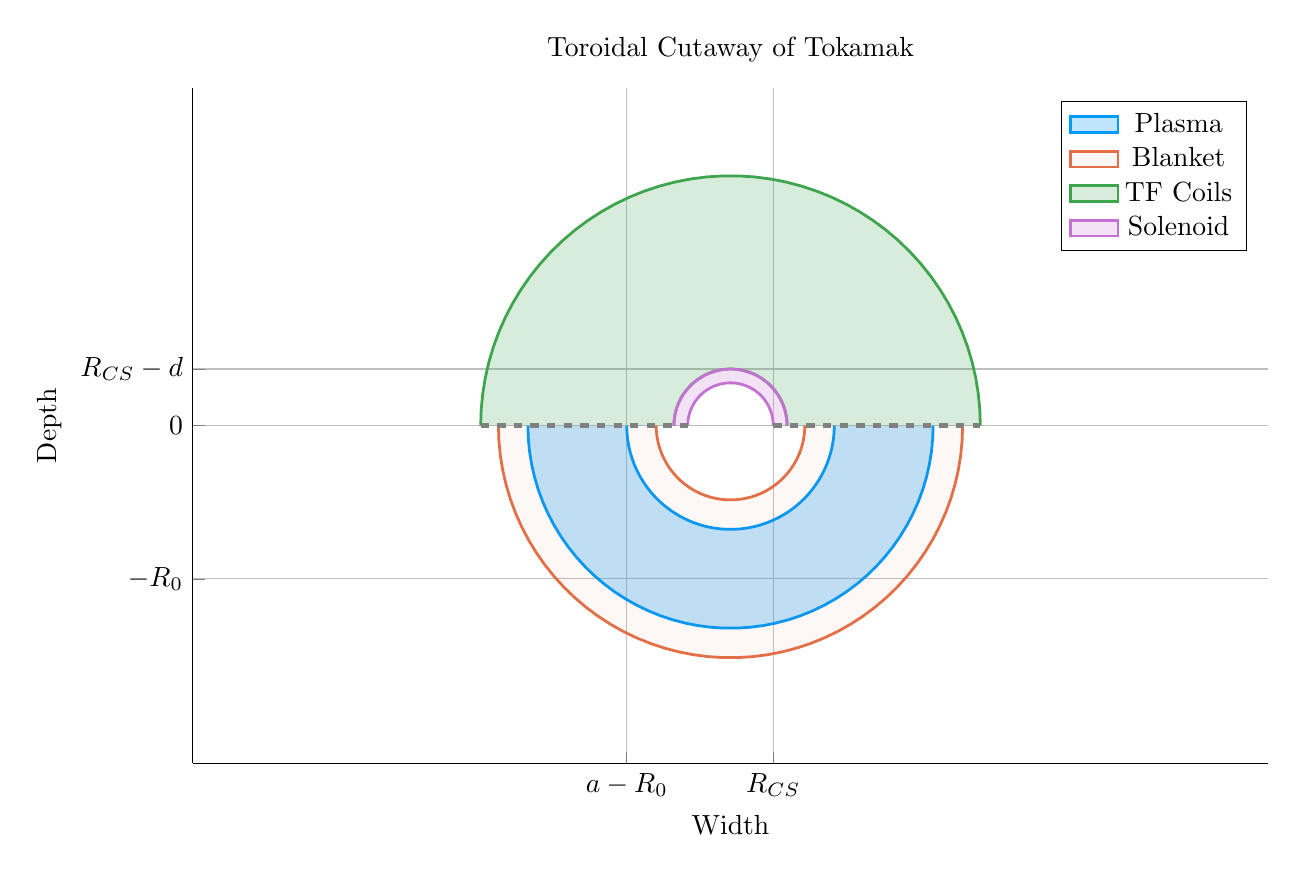
\begin{tikzpicture}[]
\begin{axis}[height = {101.6mm}, axis equal = {true}, ylabel = {Depth}, title = {Toroidal Cutaway of Tokamak}, xmin = {-30}, xmax = {30}, ymax = {20}, xlabel = {Width}, {unbounded coords=jump, scaled x ticks = false, xticklabel style={rotate = 0}, xmajorgrids = true, xtick = {2.5317214541730677,-6.145548387096774}, xticklabels = {$R_{CS}$,$a - R_0$}, xtick align = inside, axis lines* = left, scaled y ticks = false, yticklabel style={rotate = 0}, ymajorgrids = true, ytick = {0.0,-9.072,3.3497214541730678}, yticklabels = {0,${-R}_0$,$R_{CS} - d$}, ytick align = inside, axis lines* = left,     xshift = 0.0mm,
    yshift = 0.0mm,
    axis background/.style={fill={rgb,1:red,1.00000000;green,1.00000000;blue,1.00000000}}
, colorbar style={title=}}, ymin = {-20}, width = {152.4mm}]\addplot+ [color = {rgb,1:red,0.00000000;green,0.60560316;blue,0.97868012},
draw opacity=1.0,
line width=1,
solid,mark = none,
mark size = 2.0,
mark options = {
    color = {rgb,1:red,0.00000000;green,0.00000000;blue,0.00000000}, draw opacity = 1.0,
    fill = {rgb,1:red,0.00000000;green,0.60560316;blue,0.97868012}, fill opacity = 1.0,
    line width = 1,
    rotate = 0,
    solid
},fill = {rgb,1:red,0.00000000;green,0.60560316;blue,0.97868012}, fill opacity=0.25,area legend]coordinates {
(6.145548387096774, -0.0)
(6.132921698827486, -0.39374663706340574)
(6.0950935197901375, -0.7858752847367292)
(6.03221929408651, -1.1747746022953496)
(5.944557385396502, -1.5588465190247762)
(5.832468015306339, -1.9365128010360004)
(5.696411783080816, -2.3062215365670746)
(5.536947772962119, -2.666453513121427)
(5.354731256772747, -3.0157284602378778)
(5.150511001263043, -3.3526111322394856)
(4.925126191268005, -3.6757172059658885)
(4.679502981316792, -3.983718969254109)
(4.4146506898651054, -4.275350776792625)
(4.131657651789161, -4.549414250929435)
(3.831686746184227, -4.80478320606288)
(3.515970617844993, -5.040408276379846)
(3.1858066120637023, -5.255321227924983)
(2.842551443560066, -5.448638937281709)
(2.4876156214494674, -5.619567020515757)
(2.1224576531584565, -5.76740309746916)
(1.7485780511048792, -5.891539677990977)
(1.367513166770496, -5.991466658244631)
(0.9808288775031987, -6.066773416833991)
(0.5901141519911062, -6.117150502134763)
(0.19697452084939357, -6.142390903897595)
(-0.1969745208493928, -6.142390903897595)
(-0.5901141519911054, -6.117150502134763)
(-0.9808288775031978, -6.066773416833991)
(-1.3675131667704954, -5.991466658244631)
(-1.7485780511048785, -5.891539677990977)
(-2.122457653158456, -5.76740309746916)
(-2.4876156214494665, -5.619567020515757)
(-2.8425514435600636, -5.448638937281709)
(-3.1858066120637014, -5.255321227924984)
(-3.5159706178449914, -5.040408276379847)
(-3.8316867461842268, -4.804783206062881)
(-4.131657651789161, -4.549414250929435)
(-4.414650689865105, -4.275350776792626)
(-4.679502981316792, -3.983718969254109)
(-4.925126191268004, -3.675717205965889)
(-5.150511001263043, -3.3526111322394856)
(-5.354731256772745, -3.015728460237879)
(-5.536947772962118, -2.6664535131214273)
(-5.696411783080816, -2.306221536567074)
(-5.832468015306339, -1.936512801036002)
(-5.944557385396502, -1.5588465190247762)
(-6.03221929408651, -1.1747746022953511)
(-6.095093519790137, -0.7858752847367295)
(-6.132921698827486, -0.3937466370634077)
(-6.145548387096774, -7.526126161263243e-16)
(NaN, NaN)
(-11.998451612903224, -1.4693865362466332e-15)
(-11.973799507234615, -0.768743434266653)
(-11.899944491018838, -1.534327936866948)
(-11.777190050359376, -2.293607556862352)
(-11.606040609583646, -3.043462251429325)
(-11.387199458455232, -3.7808107067845746)
(-11.1215658622054, -4.502622999964288)
(-10.810231366259371, -5.205933049427548)
(-10.454475310842026, -5.887850803321573)
(-10.05575957389451, -6.545574115324709)
(-9.615722563904198, -7.176400259266735)
(-9.136172487332782, -7.777737035210403)
(-8.619079918308062, -8.347113421357031)
(-8.066569701112172, -8.882189728005088)
(-7.480912218740633, -9.380767211837053)
(-6.86451406341165, -9.840797111027321)
(-6.219908147362464, -10.260389064044016)
(-5.549743294569647, -10.637818877550004)
(-4.856773356163243, -10.971535611483144)
(-4.143845894261747, -11.260167952201693)
(-3.413890480728572, -11.502529847506192)
(-2.6699066589328715, -11.697625380382375)
(-1.9149516179824337, -11.84465286143779)
(-1.1521276300778722, -11.943008123215488)
(-0.38456930261071925, -11.992287002847684)
(0.38456930261072075, -11.992287002847684)
(1.1521276300778738, -11.943008123215488)
(1.9149516179824353, -11.84465286143779)
(2.669906658932873, -11.697625380382375)
(3.4138904807285733, -11.50252984750619)
(4.143845894261748, -11.260167952201693)
(4.856773356163245, -10.971535611483144)
(5.549743294569652, -10.637818877550002)
(6.2199081473624656, -10.260389064044015)
(6.864514063411653, -9.84079711102732)
(7.480912218740634, -9.380767211837052)
(8.06656970111217, -8.882189728005088)
(8.619079918308064, -8.34711342135703)
(9.136172487332782, -7.777737035210403)
(9.6157225639042, -7.1764002592667335)
(10.05575957389451, -6.545574115324709)
(10.45447531084203, -5.88785080332157)
(10.810231366259373, -5.205933049427547)
(11.1215658622054, -4.502622999964288)
(11.387199458455232, -3.780810706784572)
(11.606040609583646, -3.043462251429325)
(11.777190050359376, -2.293607556862349)
(11.89994449101884, -1.5343279368669474)
(11.973799507234615, -0.7687434342666493)
(11.998451612903224, -0.0)
};
\addlegendentry{Plasma}
\addplot+ [color = {rgb,1:red,0.88887350;green,0.43564919;blue,0.27812294},
draw opacity=1.0,
line width=1,
solid,mark = none,
mark size = 2.0,
mark options = {
    color = {rgb,1:red,0.00000000;green,0.00000000;blue,0.00000000}, draw opacity = 1.0,
    fill = {rgb,1:red,0.88887350;green,0.43564919;blue,0.27812294}, fill opacity = 1.0,
    line width = 1,
    rotate = 0,
    solid
},fill = {rgb,1:red,0.88887350;green,0.43564919;blue,0.27812294}, fill opacity=0.05,area legend]coordinates {
(4.399721454173068, -0.0)
(4.390681754576823, -0.28189112142273054)
(4.3635998018527395, -0.5626238917620792)
(4.31858688155362, -0.8410447198477312)
(4.255827961424217, -1.116009514776002)
(4.175580931329086, -1.3863883872247682)
(4.0781755435278235, -1.6510702924110514)
(3.964012057652294, -1.9089675956123506)
(3.8335595959539517, -2.1590205414910133)
(3.6873542155798793, -2.400201608856236)
(3.525996705798991, -2.631519732969038)
(3.350150119230053, -2.852024378039857)
(3.160537047216252, -3.0608094431839996)
(2.9579366505423685, -3.257016985784533)
(2.743181457695985, -3.4398407469625254)
(2.517153943829351, -3.608529464667722)
(2.280782904479695, -3.7623899607754563)
(2.035039638949133, -3.900789989504249)
(1.7809339590274942, -4.02316083544934)
(1.5195100394590761, -4.128999650556276)
(1.2518421272046396, -4.217871520431429)
(0.979030127130225, -4.289411251498525)
(0.7021950822621286, -4.343324871657386)
(0.4224745671806443, -4.379390838278344)
(0.14101801348210427, -4.397460948568428)
(-0.14101801348210372, -4.397460948568428)
(-0.42247456718064375, -4.379390838278344)
(-0.702195082262128, -4.343324871657387)
(-0.9790301271302244, -4.289411251498525)
(-1.2518421272046392, -4.217871520431429)
(-1.5195100394590757, -4.128999650556276)
(-1.7809339590274937, -4.02316083544934)
(-2.035039638949131, -3.9007899895042493)
(-2.2807829044796946, -3.7623899607754567)
(-2.51715394382935, -3.6085294646677224)
(-2.7431814576959845, -3.439840746962526)
(-2.957936650542369, -3.257016985784533)
(-3.1605370472162515, -3.060809443184)
(-3.350150119230053, -2.852024378039857)
(-3.5259967057989905, -2.6315197329690383)
(-3.6873542155798793, -2.400201608856236)
(-3.833559595953951, -2.1590205414910146)
(-3.9640120576522935, -1.9089675956123513)
(-4.0781755435278235, -1.6510702924110512)
(-4.175580931329086, -1.3863883872247693)
(-4.255827961424217, -1.116009514776002)
(-4.31858688155362, -0.8410447198477323)
(-4.363599801852739, -0.5626238917620795)
(-4.390681754576823, -0.2818911214227319)
(-4.399721454173068, -5.388104795992986e-16)
(NaN, NaN)
(-13.74427854582693, -1.6831886727736589e-15)
(-13.716039451485278, -0.8805989499073288)
(-13.631438208956235, -1.757579329841598)
(-13.490822462892266, -2.6273374393099704)
(-13.294770033555931, -3.4862992556780985)
(-13.044086542432483, -4.330935120595807)
(-12.739802101758393, -5.1577742441203105)
(-12.383167081569194, -5.963418966936624)
(-11.97564697166082, -6.7445587220684375)
(-11.518916359577675, -7.497983638707958)
(-11.01485204937321, -8.220597732263585)
(-10.46552534941952, -8.909431626424654)
(-9.873193560956913, -9.561654754965657)
(-9.240290702358964, -10.17458699314999)
(-8.569417507228874, -10.745709670937407)
(-7.863330737427291, -11.272675922739445)
(-7.12493185494647, -11.753320331193542)
(-6.35725509918058, -12.185667825327462)
(-5.563455018585216, -12.56794179654956)
(-4.746793507961127, -12.898571399114575)
(-3.910626404628811, -13.17619800506574)
(-3.0583896985731425, -13.39968078712848)
(-2.1935854132235035, -13.568101406614394)
(-1.319767214888334, -13.680767787071906)
(-0.4405258099780083, -13.737216958176852)
(0.44052580997801, -13.737216958176852)
(1.3197672148883357, -13.680767787071906)
(2.1935854132235053, -13.568101406614392)
(3.058389698573144, -13.39968078712848)
(3.9106264046288124, -13.176198005065737)
(4.7467935079611285, -12.898571399114575)
(5.563455018585217, -12.56794179654956)
(6.357255099180584, -12.18566782532746)
(7.124931854946472, -11.75332033119354)
(7.863330737427294, -11.272675922739444)
(8.569417507228875, -10.745709670937405)
(9.240290702358962, -10.17458699314999)
(9.873193560956915, -9.561654754965655)
(10.46552534941952, -8.909431626424654)
(11.014852049373212, -8.220597732263583)
(11.518916359577675, -7.497983638707958)
(11.975646971660824, -6.744558722068434)
(12.383167081569196, -5.963418966936623)
(12.739802101758393, -5.157774244120311)
(13.044086542432483, -4.330935120595804)
(13.294770033555931, -3.4862992556780985)
(13.490822462892266, -2.6273374393099673)
(13.631438208956236, -1.7575793298415974)
(13.716039451485278, -0.8805989499073243)
(13.74427854582693, -0.0)
};
\addlegendentry{Blanket}
\addplot+ [color = {rgb,1:red,0.24222430;green,0.64327509;blue,0.30444865},
draw opacity=1.0,
line width=1,
solid,mark = none,
mark size = 2.0,
mark options = {
    color = {rgb,1:red,0.00000000;green,0.00000000;blue,0.00000000}, draw opacity = 1.0,
    fill = {rgb,1:red,0.24222430;green,0.64327509;blue,0.30444865}, fill opacity = 1.0,
    line width = 1,
    rotate = 0,
    solid
},fill = {rgb,1:red,0.24222430;green,0.64327509;blue,0.30444865}, fill opacity=0.2,area legend]coordinates {
(3.3497214541730678, 0.0)
(3.34283909218897, 0.214617390442982)
(3.322220287338331, 0.42835287199334793)
(3.2879497667130018, 0.6403281597112903)
(3.2401683552332363, 0.8496722016710194)
(3.179072396967884, 1.0555247582999667)
(3.1049129483145004, 1.2570399372877088)
(3.017994746354754, 1.4533896695389148)
(2.918674956624393, 1.6437671118868786)
(2.807361705443447, 1.8273899625851602)
(2.684512402837637, 2.003503675953261)
(2.550631862942462, 2.1713845629666793)
(2.4062702296136385, 2.330342765050339)
(2.252020715767986, 2.4797250888554516)
(2.088517165744315, 2.6189176903710942)
(1.916431450701073, 2.7473485973409186)
(1.7364707077536436, 2.864490059619843)
(1.5493744341962556, 2.969860717812599)
(1.3559114487489807, 3.0630275812827366)
(1.1568767323167033, 3.143607807404028)
(0.9530881612420555, 3.2112702747429354)
(0.7453831464760948, 3.265736943707611)
(0.5346151924770803, 3.306783999072214)
(0.32165038997757833, 3.3342427696816865)
(0.10736385703186618, 3.3480004215577055)
(-0.10736385703186577, 3.3480004215577055)
(-0.3216503899775779, 3.3342427696816865)
(-0.5346151924770799, 3.3067839990722145)
(-0.7453831464760944, 3.265736943707611)
(-0.9530881612420552, 3.211270274742936)
(-1.1568767323167028, 3.143607807404028)
(-1.3559114487489803, 3.0630275812827366)
(-1.5493744341962545, 2.9698607178125993)
(-1.7364707077536434, 2.8644900596198433)
(-1.9164314507010722, 2.747348597340919)
(-2.0885171657443147, 2.6189176903710947)
(-2.2520207157679866, 2.4797250888554516)
(-2.406270229613638, 2.3303427650503394)
(-2.550631862942462, 2.1713845629666793)
(-2.6845124028376364, 2.003503675953261)
(-2.807361705443447, 1.8273899625851602)
(-2.9186749566243924, 1.6437671118868797)
(-3.017994746354754, 1.453389669538915)
(-3.1049129483145004, 1.2570399372877086)
(-3.179072396967884, 1.0555247582999674)
(-3.2401683552332363, 0.8496722016710194)
(-3.2879497667130018, 0.6403281597112912)
(-3.3222202873383306, 0.4283528719933481)
(-3.34283909218897, 0.21461739044298306)
(-3.3497214541730678, 4.1022256568882646e-16)
(NaN, NaN)
(-14.79427854582693, 1.811776586684131e-15)
(-14.76388211387313, 0.9478726808870777)
(-14.672817723470644, 1.8918503496103294)
(-14.521459577732886, 2.828053999446412)
(-14.310429639746912, 3.7526365687830814)
(-14.040595076793686, 4.661798749520609)
(-13.713064696971717, 5.5518045992436535)
(-13.329184392866736, 6.4189968930100605)
(-12.89053161099038, 7.259812151672573)
(-12.398908869714107, 8.070795284979035)
(-11.856336352334566, 8.848613789279362)
(-11.265043605707111, 9.590071441497832)
(-10.627460378559528, 10.292121433099318)
(-9.946206637133345, 10.95187889007907)
(-9.224081799180544, 11.56663272752884)
(-8.46405323055557, 12.133856790066249)
(-7.669244051672522, 12.651220232349157)
(-6.8429203039334565, 13.116597097019113)
(-5.988477528863729, 13.528075050716163)
(-5.109426815103499, 13.883963242266825)
(-4.209380370591395, 14.182799250754234)
(-3.2920366792272726, 14.423355094919396)
(-2.3611653030085518, 14.604642279199568)
(-1.4205913920913997, 14.725915855668564)
(-0.4741799664282463, 14.786677485187575)
(0.4741799664282481, 14.786677485187575)
(1.4205913920914017, 14.725915855668564)
(2.3611653030085535, 14.604642279199567)
(3.2920366792272744, 14.423355094919396)
(4.209380370591397, 14.182799250754233)
(5.109426815103501, 13.883963242266825)
(5.988477528863731, 13.528075050716163)
(6.842920303933462, 13.116597097019111)
(7.669244051672524, 12.651220232349155)
(8.464053230555573, 12.133856790066247)
(9.224081799180546, 11.566632727528837)
(9.946206637133345, 10.95187889007907)
(10.62746037855953, 10.292121433099316)
(11.265043605707111, 9.590071441497832)
(11.856336352334568, 8.84861378927936)
(12.398908869714107, 8.070795284979035)
(12.890531610990383, 7.259812151672569)
(13.329184392866738, 6.418996893010059)
(13.713064696971717, 5.551804599243654)
(14.040595076793686, 4.661798749520606)
(14.310429639746912, 3.7526365687830814)
(14.521459577732886, 2.828053999446408)
(14.672817723470645, 1.8918503496103287)
(14.76388211387313, 0.947872680887073)
(14.79427854582693, 0.0)
};
\addlegendentry{TF Coils}
\addplot+ [color = {rgb,1:red,0.76444018;green,0.44411178;blue,0.82429754},
draw opacity=1.0,
line width=1,
solid,mark = none,
mark size = 2.0,
mark options = {
    color = {rgb,1:red,0.00000000;green,0.00000000;blue,0.00000000}, draw opacity = 1.0,
    fill = {rgb,1:red,0.76444018;green,0.44411178;blue,0.82429754}, fill opacity = 1.0,
    line width = 1,
    rotate = 0,
    solid
},fill = {rgb,1:red,0.76444018;green,0.44411178;blue,0.82429754}, fill opacity=0.2,area legend]coordinates {
(2.5317214541730677, 0.0)
(2.5265197609191947, 0.16220795049875883)
(2.5109360560309155, 0.323749353735422)
(2.4850343762943106, 0.4839604014335678)
(2.44892115726731, 0.6421827520330423)
(2.402744795913157, 0.797766235956645)
(2.3466950408054545, 0.9500715272963807)
(2.2810022124105753, 1.0984727709407522)
(2.2059362566514604, 1.2423601543476575)
(2.121805635641921, 1.3811424133949313)
(2.0289560601496484, 1.5142492620114463)
(1.9277690689965101, 1.6411337356049083)
(1.818660461233697, 1.7612744386566872)
(1.702078587534229, 1.8741776872478437)
(1.5785025078238708, 1.9793795377122456)
(1.448440022721138, 2.076447693080609)
(1.312425586875634, 2.16498327948147)
(1.1710181127792523, 2.2446224851994847)
(1.0247986740748627, 2.315038055655802)
(0.8743681178000735, 2.375940638167324)
(0.720344595377871, 2.427079970958947)
(0.5633610224998296, 2.4682459115428794)
(0.40406247833977604, 2.499269300239194)
(0.24310355478509454, 2.5200226552892424)
(0.08114566657825212, 2.5304206967055425)
(-0.0811456665782518, 2.5304206967055425)
(-0.2431035547850942, 2.5200226552892424)
(-0.4040624783397757, 2.4992693002391944)
(-0.5633610224998293, 2.4682459115428794)
(-0.7203445953778707, 2.4270799709589475)
(-0.8743681178000733, 2.375940638167324)
(-1.0247986740748622, 2.315038055655802)
(-1.1710181127792514, 2.244622485199485)
(-1.3124255868756338, 2.1649832794814703)
(-1.4484400227211376, 2.076447693080609)
(-1.5785025078238706, 1.979379537712246)
(-1.7020785875342292, 1.8741776872478437)
(-1.8186604612336967, 1.7612744386566876)
(-1.9277690689965101, 1.6411337356049083)
(-2.028956060149648, 1.5142492620114465)
(-2.121805635641921, 1.3811424133949313)
(-2.20593625665146, 1.2423601543476581)
(-2.281002212410575, 1.0984727709407525)
(-2.3466950408054545, 0.9500715272963806)
(-2.402744795913157, 0.7977662359566455)
(-2.44892115726731, 0.6421827520330423)
(-2.4850343762943106, 0.4839604014335684)
(-2.5109360560309155, 0.3237493537354222)
(-2.5265197609191947, 0.16220795049875963)
(-2.5317214541730677, 3.1004645751857297e-16)
(NaN, NaN)
(-3.3497214541730678, 4.1022256568882646e-16)
(-3.34283909218897, 0.21461739044298306)
(-3.3222202873383306, 0.4283528719933481)
(-3.2879497667130018, 0.6403281597112912)
(-3.2401683552332363, 0.8496722016710194)
(-3.179072396967884, 1.0555247582999674)
(-3.1049129483145004, 1.2570399372877086)
(-3.017994746354754, 1.453389669538915)
(-2.9186749566243924, 1.6437671118868797)
(-2.807361705443447, 1.8273899625851602)
(-2.6845124028376364, 2.003503675953261)
(-2.550631862942462, 2.1713845629666793)
(-2.406270229613638, 2.3303427650503394)
(-2.2520207157679866, 2.4797250888554516)
(-2.0885171657443147, 2.6189176903710947)
(-1.9164314507010722, 2.747348597340919)
(-1.7364707077536434, 2.8644900596198433)
(-1.5493744341962545, 2.9698607178125993)
(-1.3559114487489803, 3.0630275812827366)
(-1.1568767323167028, 3.143607807404028)
(-0.9530881612420552, 3.211270274742936)
(-0.7453831464760944, 3.265736943707611)
(-0.5346151924770799, 3.3067839990722145)
(-0.3216503899775779, 3.3342427696816865)
(-0.10736385703186577, 3.3480004215577055)
(0.10736385703186618, 3.3480004215577055)
(0.32165038997757833, 3.3342427696816865)
(0.5346151924770803, 3.306783999072214)
(0.7453831464760948, 3.265736943707611)
(0.9530881612420555, 3.2112702747429354)
(1.1568767323167033, 3.143607807404028)
(1.3559114487489807, 3.0630275812827366)
(1.5493744341962556, 2.969860717812599)
(1.7364707077536436, 2.864490059619843)
(1.916431450701073, 2.7473485973409186)
(2.088517165744315, 2.6189176903710942)
(2.252020715767986, 2.4797250888554516)
(2.4062702296136385, 2.330342765050339)
(2.550631862942462, 2.1713845629666793)
(2.684512402837637, 2.003503675953261)
(2.807361705443447, 1.8273899625851602)
(2.918674956624393, 1.6437671118868786)
(3.017994746354754, 1.4533896695389148)
(3.1049129483145004, 1.2570399372877088)
(3.179072396967884, 1.0555247582999667)
(3.2401683552332363, 0.8496722016710194)
(3.2879497667130018, 0.6403281597112903)
(3.322220287338331, 0.42835287199334793)
(3.34283909218897, 0.214617390442982)
(3.3497214541730678, 0.0)
};
\addlegendentry{Solenoid}
\addplot+ [color = {rgb,1:red,0.50196078;green,0.50196078;blue,0.50196078},
draw opacity=1.0,
line width=2,
dashed,mark = none,
mark size = 2.0,
mark options = {
    color = {rgb,1:red,0.00000000;green,0.00000000;blue,0.00000000}, draw opacity = 1.0,
    fill = {rgb,1:red,0.50196078;green,0.50196078;blue,0.50196078}, fill opacity = 1.0,
    line width = 1,
    rotate = 0,
    solid
},forget plot]coordinates {
(-14.79427854582693, 0.0)
(-2.5317214541730677, 0.0)
(NaN, NaN)
(2.5317214541730677, 0.0)
(14.79427854582693, 0.0)
};
\end{axis}

\end{tikzpicture}

		\end{adjustbox}
        \caption{Toroidal Cutaway}
    \end{subfigure}
    \hfill
    \begin{subfigure}[t]{0.45\textwidth}
        \centering
		\begin{adjustbox}{width=\textwidth}
			\Large
			\begin{adjustbox}{width=0.85\textwidth}
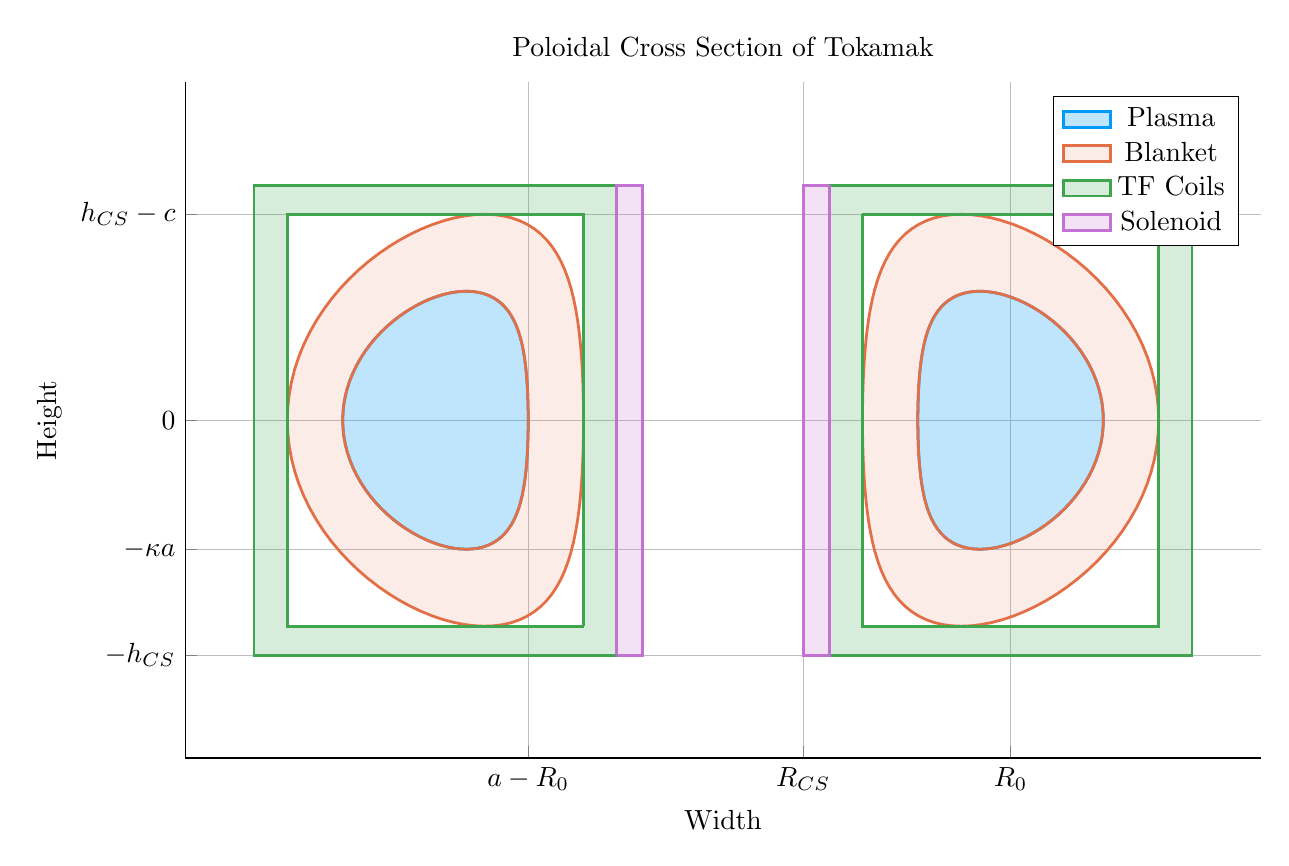
\begin{tikzpicture}[]
\begin{axis}[height = {101.6mm}, ylabel = {Height}, title = {Poloidal Cross Section of Tokamak}, xmin = {-16.96464}, xmax = {16.96464}, ymax = {12.181706012903225}, xlabel = {Width}, unbounded coords=jump,scaled x ticks = false,xticklabel style={rotate = 0},xmajorgrids = true,xtick = {9.072,-6.145548387096774,2.5317214541730677},xticklabels = {${{R}_0}$,$a - R_0$,$R_{CS}$},xtick align = inside,axis lines* = left,scaled y ticks = false,yticklabel style={rotate = 0},ymajorgrids = true,ytick = {0.0,-8.478922887864822,-4.653058064516129,7.428922887864823},yticklabels = {0,${{-h}_{CS}}$,${-\kappa} a$,$h_{CS} - c$},ytick align = inside,axis lines* = left,    xshift = 0.0mm,
    yshift = 0.0mm,
    axis background/.style={fill={rgb,1:red,1.00000000;green,1.00000000;blue,1.00000000}}
, ymin = {-12.181706012903225}, width = {152.4mm}]\addplot+ [color = {rgb,1:red,0.00000000;green,0.60560316;blue,0.97868012},
draw opacity=1.0,
line width=1,
solid,mark = none,
mark size = 2.0,
mark options = {
    color = {rgb,1:red,0.00000000;green,0.00000000;blue,0.00000000}, draw opacity = 1.0,
    fill = {rgb,1:red,0.00000000;green,0.60560316;blue,0.97868012}, fill opacity = 1.0,
    line width = 1,
    rotate = 0,
    solid
},fill = {rgb,1:red,0.00000000;green,0.60560316;blue,0.97868012}, fill opacity=0.25,area legend]coordinates {
(-11.998451612903224, 0.0)
(-11.98922207919679, 0.2921679332710291)
(-11.961601612443932, 0.5831828131882695)
(-11.915794116436746, 0.8718961369727396)
(-11.852137762522407, 1.1571684850360338)
(-11.771102473770108, 1.4378740177488842)
(-11.673286377647635, 1.7129049186158334)
(-11.55941120568557, 1.9811757663208256)
(-11.430316617462449, 2.241627818389261)
(-11.286953428530017, 2.4932331895608506)
(-11.130375728034215, 2.7349989083831394)
(-10.96173188200961, 2.9659708360161865)
(-10.782254432669117, 3.1852374317826615)
(-10.59324892230544, 3.391933350602452)
(-10.396081692289423, 3.58524285811436)
(-10.192166732519574, 3.7644030500069485)
(-9.982951683794182, 3.9287068628533244)
(-9.769903124035281, 4.0775058645674545)
(-9.554491298062636, 4.21021281346937)
(-9.338174478579997, 4.326303975859794)
(-9.122383172034585, 4.425321192957779)
(-8.908504405883159, 4.5068736890441015)
(-8.697866352426912, 4.570639613674501)
(-8.491723557735288, 4.616367311876341)
(-8.2912430513685, 4.643876317315818)
(-8.097491612903225, 4.653058064516129)
(-7.911424464141755, 4.643876317315818)
(-7.73387564104738, 4.616367311876341)
(-7.565550276852846, 4.570639613674501)
(-7.4070189976483904, 4.506873689044102)
(-7.258714594546428, 4.42532119295778)
(-7.120931092970638, 4.326303975859795)
(-6.993825290693801, 4.21021281346937)
(-6.877420783129728, 4.077505864567455)
(-6.771614438426758, 3.928706862853325)
(-6.676185227609827, 3.7644030500069485)
(-6.590805257964794, 3.58524285811436)
(-6.515052802686304, 3.391933350602452)
(-6.448427068145589, 3.1852374317826624)
(-6.390364393542622, 2.9659708360161874)
(-6.340255537642832, 2.73499890838314)
(-6.297463675055492, 2.4932331895608506)
(-6.261342701178994, 2.241627818389261)
(-6.231255431364441, 1.9811757663208265)
(-6.206591276608178, 1.7129049186158343)
(-6.186782985455325, 1.4378740177488847)
(-6.171322059752492, 1.1571684850360338)
(-6.159772480089943, 0.8718961369727395)
(-6.151782414579849, 0.5831828131882707)
(-6.147093631099405, 0.29216793327103)
(-6.145548387096774, 5.698352664956456e-16)
(-6.147093631099405, -0.2921679332710289)
(-6.151782414579849, -0.5831828131882696)
(-6.159772480089943, -0.8718961369727383)
(-6.171322059752492, -1.1571684850360326)
(-6.1867829854553245, -1.4378740177488838)
(-6.206591276608178, -1.7129049186158334)
(-6.231255431364441, -1.9811757663208256)
(-6.261342701178992, -2.2416278183892597)
(-6.297463675055493, -2.4932331895608497)
(-6.340255537642832, -2.734998908383139)
(-6.390364393542622, -2.9659708360161865)
(-6.448427068145589, -3.185237431782662)
(-6.515052802686304, -3.3919333506024514)
(-6.590805257964794, -3.5852428581143605)
(-6.676185227609827, -3.7644030500069485)
(-6.771614438426755, -3.928706862853323)
(-6.877420783129727, -4.0775058645674545)
(-6.9938252906938, -4.21021281346937)
(-7.120931092970639, -4.326303975859795)
(-7.258714594546428, -4.425321192957779)
(-7.407018997648389, -4.5068736890441015)
(-7.565550276852846, -4.570639613674501)
(-7.733875641047377, -4.616367311876341)
(-7.9114244641417555, -4.643876317315818)
(-8.097491612903225, -4.653058064516129)
(-8.291243051368498, -4.643876317315818)
(-8.491723557735288, -4.616367311876341)
(-8.69786635242691, -4.570639613674501)
(-8.90850440588316, -4.5068736890441015)
(-9.122383172034585, -4.42532119295778)
(-9.338174478579994, -4.326303975859796)
(-9.554491298062636, -4.21021281346937)
(-9.76990312403528, -4.077505864567455)
(-9.982951683794184, -3.928706862853324)
(-10.192166732519574, -3.7644030500069494)
(-10.396081692289421, -3.5852428581143614)
(-10.59324892230544, -3.391933350602452)
(-10.782254432669115, -3.1852374317826624)
(-10.96173188200961, -2.9659708360161865)
(-11.130375728034215, -2.7349989083831403)
(-11.286953428530017, -2.493233189560853)
(-11.430316617462449, -2.241627818389261)
(-11.559411205685569, -1.981175766320827)
(-11.673286377647635, -1.7129049186158327)
(-11.771102473770108, -1.4378740177488853)
(-11.852137762522407, -1.1571684850360362)
(-11.915794116436746, -0.8718961369727398)
(-11.961601612443932, -0.5831828131882713)
(-11.98922207919679, -0.2921679332710286)
(-11.998451612903224, -1.1396705329912913e-15)
(NaN, NaN)
(11.998451612903224, 0.0)
(11.98922207919679, 0.2921679332710291)
(11.961601612443932, 0.5831828131882695)
(11.915794116436746, 0.8718961369727396)
(11.852137762522407, 1.1571684850360338)
(11.771102473770108, 1.4378740177488842)
(11.673286377647635, 1.7129049186158334)
(11.55941120568557, 1.9811757663208256)
(11.430316617462449, 2.241627818389261)
(11.286953428530017, 2.4932331895608506)
(11.130375728034215, 2.7349989083831394)
(10.96173188200961, 2.9659708360161865)
(10.782254432669117, 3.1852374317826615)
(10.59324892230544, 3.391933350602452)
(10.396081692289423, 3.58524285811436)
(10.192166732519574, 3.7644030500069485)
(9.982951683794182, 3.9287068628533244)
(9.769903124035281, 4.0775058645674545)
(9.554491298062636, 4.21021281346937)
(9.338174478579997, 4.326303975859794)
(9.122383172034585, 4.425321192957779)
(8.908504405883159, 4.5068736890441015)
(8.697866352426912, 4.570639613674501)
(8.491723557735288, 4.616367311876341)
(8.2912430513685, 4.643876317315818)
(8.097491612903225, 4.653058064516129)
(7.911424464141755, 4.643876317315818)
(7.73387564104738, 4.616367311876341)
(7.565550276852846, 4.570639613674501)
(7.4070189976483904, 4.506873689044102)
(7.258714594546428, 4.42532119295778)
(7.120931092970638, 4.326303975859795)
(6.993825290693801, 4.21021281346937)
(6.877420783129728, 4.077505864567455)
(6.771614438426758, 3.928706862853325)
(6.676185227609827, 3.7644030500069485)
(6.590805257964794, 3.58524285811436)
(6.515052802686304, 3.391933350602452)
(6.448427068145589, 3.1852374317826624)
(6.390364393542622, 2.9659708360161874)
(6.340255537642832, 2.73499890838314)
(6.297463675055492, 2.4932331895608506)
(6.261342701178994, 2.241627818389261)
(6.231255431364441, 1.9811757663208265)
(6.206591276608178, 1.7129049186158343)
(6.186782985455325, 1.4378740177488847)
(6.171322059752492, 1.1571684850360338)
(6.159772480089943, 0.8718961369727395)
(6.151782414579849, 0.5831828131882707)
(6.147093631099405, 0.29216793327103)
(6.145548387096774, 5.698352664956456e-16)
(6.147093631099405, -0.2921679332710289)
(6.151782414579849, -0.5831828131882696)
(6.159772480089943, -0.8718961369727383)
(6.171322059752492, -1.1571684850360326)
(6.1867829854553245, -1.4378740177488838)
(6.206591276608178, -1.7129049186158334)
(6.231255431364441, -1.9811757663208256)
(6.261342701178992, -2.2416278183892597)
(6.297463675055493, -2.4932331895608497)
(6.340255537642832, -2.734998908383139)
(6.390364393542622, -2.9659708360161865)
(6.448427068145589, -3.185237431782662)
(6.515052802686304, -3.3919333506024514)
(6.590805257964794, -3.5852428581143605)
(6.676185227609827, -3.7644030500069485)
(6.771614438426755, -3.928706862853323)
(6.877420783129727, -4.0775058645674545)
(6.9938252906938, -4.21021281346937)
(7.120931092970639, -4.326303975859795)
(7.258714594546428, -4.425321192957779)
(7.407018997648389, -4.5068736890441015)
(7.565550276852846, -4.570639613674501)
(7.733875641047377, -4.616367311876341)
(7.9114244641417555, -4.643876317315818)
(8.097491612903225, -4.653058064516129)
(8.291243051368498, -4.643876317315818)
(8.491723557735288, -4.616367311876341)
(8.69786635242691, -4.570639613674501)
(8.90850440588316, -4.5068736890441015)
(9.122383172034585, -4.42532119295778)
(9.338174478579994, -4.326303975859796)
(9.554491298062636, -4.21021281346937)
(9.76990312403528, -4.077505864567455)
(9.982951683794184, -3.928706862853324)
(10.192166732519574, -3.7644030500069494)
(10.396081692289421, -3.5852428581143614)
(10.59324892230544, -3.391933350602452)
(10.782254432669115, -3.1852374317826624)
(10.96173188200961, -2.9659708360161865)
(11.130375728034215, -2.7349989083831403)
(11.286953428530017, -2.493233189560853)
(11.430316617462449, -2.241627818389261)
(11.559411205685569, -1.981175766320827)
(11.673286377647635, -1.7129049186158327)
(11.771102473770108, -1.4378740177488853)
(11.852137762522407, -1.1571684850360362)
(11.915794116436746, -0.8718961369727398)
(11.961601612443932, -0.5831828131882713)
(11.98922207919679, -0.2921679332710286)
(11.998451612903224, -1.1396705329912913e-15)
};
\addlegendentry{Plasma}
\addplot+ [color = {rgb,1:red,0.88887350;green,0.43564919;blue,0.27812294},
draw opacity=1.0,
line width=1,
solid,mark = none,
mark size = 2.0,
mark options = {
    color = {rgb,1:red,0.00000000;green,0.00000000;blue,0.00000000}, draw opacity = 1.0,
    fill = {rgb,1:red,0.88887350;green,0.43564919;blue,0.27812294}, fill opacity = 1.0,
    line width = 1,
    rotate = 0,
    solid
},fill = {rgb,1:red,0.88887350;green,0.43564919;blue,0.27812294}, fill opacity=0.125,area legend]coordinates {
(-13.74427854582693, 0.0)
(-13.72954296908463, 0.46646592767223927)
(-13.685445019996358, 0.9310909274359673)
(-13.612310244800092, 1.392041336684088)
(-13.510678556994915, 1.8474979947395098)
(-13.381300220642846, 2.2956634222512418)
(-13.225130186826302, 2.734768915024204)
(-13.04332074889991, 3.1630815242866377)
(-12.837212480347718, 3.5789108958472036)
(-12.608323422706404, 3.9806159411507194)
(-12.358336500812388, 4.3666113139049525)
(-12.08908515895104, 4.735373666718153)
(-11.802537234387401, 5.08544766305526)
(-11.500777113966619, 5.4154517207863275)
(-11.185986254387002, 5.724083464660006)
(-10.860422186454013, 6.010124866183653)
(-10.526396166917667, 6.272447050625345)
(-10.18624968693083, 6.510014752166694)
(-9.842330092097374, 6.721890399624077)
(-9.496965613725703, 6.907237816613755)
(-9.152440152411872, 7.065325521558049)
(-8.81096819159381, 7.195529614508949)
(-8.474670248460548, 7.297336239396166)
(-8.14554929092694, 7.370343611982296)
(-7.825468560863273, 7.4142636055216355)
(-7.516131244239631, 7.428922887864823)
(-7.2190624174706315, 7.4142636055216355)
(-6.935593675557043, 7.370343611982296)
(-6.666850811544881, 7.297336239396167)
(-6.4137448687014755, 7.195529614508949)
(-6.176966827400615, 7.065325521558051)
(-5.956986119179431, 6.907237816613756)
(-5.754053082320152, 6.721890399624076)
(-5.568205388501765, 6.510014752166695)
(-5.3992783807260825, 6.272447050625345)
(-5.246919171238659, 6.010124866183653)
(-5.110604257075394, 5.724083464660006)
(-4.989660322779391, 5.4154517207863275)
(-4.88328781734585, 5.085447663055262)
(-4.790586818065825, 4.735373666718154)
(-4.7105846299742, 4.366611313904953)
(-4.642264518129107, 3.9806159411507194)
(-4.584594932698949, 3.578910895847203)
(-4.536558565161822, 3.1630815242866395)
(-4.497180568747824, 2.7347689150242047)
(-4.465555288023927, 2.2956634222512426)
(-4.440870871189059, 1.8474979947395103)
(-4.422431183673739, 1.3920413366840876)
(-4.409674501998921, 0.9310909274359696)
(-4.402188541060726, 0.46646592767224077)
(-4.399721454173068, 9.097806635736167e-16)
(-4.402188541060726, -0.466465927672239)
(-4.409674501998921, -0.9310909274359678)
(-4.422431183673739, -1.392041336684086)
(-4.440870871189059, -1.8474979947395083)
(-4.465555288023926, -2.295663422251241)
(-4.497180568747823, -2.734768915024204)
(-4.536558565161822, -3.1630815242866377)
(-4.5845949326989475, -3.5789108958472013)
(-4.642264518129108, -3.980615941150719)
(-4.7105846299742, -4.3666113139049525)
(-4.790586818065825, -4.735373666718153)
(-4.88328781734585, -5.085447663055261)
(-4.989660322779391, -5.415451720786327)
(-5.110604257075395, -5.724083464660007)
(-5.246919171238659, -6.010124866183653)
(-5.399278380726081, -6.272447050625343)
(-5.568205388501764, -6.510014752166694)
(-5.754053082320152, -6.721890399624076)
(-5.956986119179432, -6.907237816613756)
(-6.176966827400615, -7.065325521558049)
(-6.413744868701472, -7.195529614508947)
(-6.666850811544881, -7.297336239396167)
(-6.935593675557041, -7.370343611982296)
(-7.219062417470632, -7.4142636055216355)
(-7.51613124423963, -7.428922887864823)
(-7.8254685608632695, -7.4142636055216355)
(-8.14554929092694, -7.370343611982296)
(-8.474670248460544, -7.297336239396167)
(-8.810968191593812, -7.195529614508949)
(-9.152440152411872, -7.065325521558051)
(-9.4969656137257, -6.9072378166137565)
(-9.842330092097372, -6.721890399624077)
(-10.186249686930825, -6.510014752166696)
(-10.526396166917669, -6.272447050625344)
(-10.860422186454013, -6.010124866183654)
(-11.185986254386998, -5.724083464660007)
(-11.500777113966619, -5.4154517207863275)
(-11.8025372343874, -5.085447663055262)
(-12.08908515895104, -4.735373666718153)
(-12.358336500812388, -4.366611313904954)
(-12.608323422706402, -3.9806159411507234)
(-12.837212480347718, -3.5789108958472036)
(-13.04332074889991, -3.1630815242866404)
(-13.225130186826302, -2.7347689150242034)
(-13.381300220642846, -2.2956634222512435)
(-13.510678556994915, -1.8474979947395136)
(-13.612310244800092, -1.3920413366840885)
(-13.685445019996358, -0.9310909274359703)
(-13.72954296908463, -0.46646592767223843)
(-13.74427854582693, -1.8195613271472333e-15)
(NaN, NaN)
(13.74427854582693, 0.0)
(13.72954296908463, 0.46646592767223927)
(13.685445019996358, 0.9310909274359673)
(13.612310244800092, 1.392041336684088)
(13.510678556994915, 1.8474979947395098)
(13.381300220642846, 2.2956634222512418)
(13.225130186826302, 2.734768915024204)
(13.04332074889991, 3.1630815242866377)
(12.837212480347718, 3.5789108958472036)
(12.608323422706404, 3.9806159411507194)
(12.358336500812388, 4.3666113139049525)
(12.08908515895104, 4.735373666718153)
(11.802537234387401, 5.08544766305526)
(11.500777113966619, 5.4154517207863275)
(11.185986254387002, 5.724083464660006)
(10.860422186454013, 6.010124866183653)
(10.526396166917667, 6.272447050625345)
(10.18624968693083, 6.510014752166694)
(9.842330092097374, 6.721890399624077)
(9.496965613725703, 6.907237816613755)
(9.152440152411872, 7.065325521558049)
(8.81096819159381, 7.195529614508949)
(8.474670248460548, 7.297336239396166)
(8.14554929092694, 7.370343611982296)
(7.825468560863273, 7.4142636055216355)
(7.516131244239631, 7.428922887864823)
(7.2190624174706315, 7.4142636055216355)
(6.935593675557043, 7.370343611982296)
(6.666850811544881, 7.297336239396167)
(6.4137448687014755, 7.195529614508949)
(6.176966827400615, 7.065325521558051)
(5.956986119179431, 6.907237816613756)
(5.754053082320152, 6.721890399624076)
(5.568205388501765, 6.510014752166695)
(5.3992783807260825, 6.272447050625345)
(5.246919171238659, 6.010124866183653)
(5.110604257075394, 5.724083464660006)
(4.989660322779391, 5.4154517207863275)
(4.88328781734585, 5.085447663055262)
(4.790586818065825, 4.735373666718154)
(4.7105846299742, 4.366611313904953)
(4.642264518129107, 3.9806159411507194)
(4.584594932698949, 3.578910895847203)
(4.536558565161822, 3.1630815242866395)
(4.497180568747824, 2.7347689150242047)
(4.465555288023927, 2.2956634222512426)
(4.440870871189059, 1.8474979947395103)
(4.422431183673739, 1.3920413366840876)
(4.409674501998921, 0.9310909274359696)
(4.402188541060726, 0.46646592767224077)
(4.399721454173068, 9.097806635736167e-16)
(4.402188541060726, -0.466465927672239)
(4.409674501998921, -0.9310909274359678)
(4.422431183673739, -1.392041336684086)
(4.440870871189059, -1.8474979947395083)
(4.465555288023926, -2.295663422251241)
(4.497180568747823, -2.734768915024204)
(4.536558565161822, -3.1630815242866377)
(4.5845949326989475, -3.5789108958472013)
(4.642264518129108, -3.980615941150719)
(4.7105846299742, -4.3666113139049525)
(4.790586818065825, -4.735373666718153)
(4.88328781734585, -5.085447663055261)
(4.989660322779391, -5.415451720786327)
(5.110604257075395, -5.724083464660007)
(5.246919171238659, -6.010124866183653)
(5.399278380726081, -6.272447050625343)
(5.568205388501764, -6.510014752166694)
(5.754053082320152, -6.721890399624076)
(5.956986119179432, -6.907237816613756)
(6.176966827400615, -7.065325521558049)
(6.413744868701472, -7.195529614508947)
(6.666850811544881, -7.297336239396167)
(6.935593675557041, -7.370343611982296)
(7.219062417470632, -7.4142636055216355)
(7.51613124423963, -7.428922887864823)
(7.8254685608632695, -7.4142636055216355)
(8.14554929092694, -7.370343611982296)
(8.474670248460544, -7.297336239396167)
(8.810968191593812, -7.195529614508949)
(9.152440152411872, -7.065325521558051)
(9.4969656137257, -6.9072378166137565)
(9.842330092097372, -6.721890399624077)
(10.186249686930825, -6.510014752166696)
(10.526396166917669, -6.272447050625344)
(10.860422186454013, -6.010124866183654)
(11.185986254386998, -5.724083464660007)
(11.500777113966619, -5.4154517207863275)
(11.8025372343874, -5.085447663055262)
(12.08908515895104, -4.735373666718153)
(12.358336500812388, -4.366611313904954)
(12.608323422706402, -3.9806159411507234)
(12.837212480347718, -3.5789108958472036)
(13.04332074889991, -3.1630815242866404)
(13.225130186826302, -2.7347689150242034)
(13.381300220642846, -2.2956634222512435)
(13.510678556994915, -1.8474979947395136)
(13.612310244800092, -1.3920413366840885)
(13.685445019996358, -0.9310909274359703)
(13.72954296908463, -0.46646592767223843)
(13.74427854582693, -1.8195613271472333e-15)
(NaN, NaN)
(11.998451612903224, -1.1396705329912913e-15)
(11.98922207919679, -0.2921679332710286)
(11.961601612443932, -0.5831828131882713)
(11.915794116436746, -0.8718961369727398)
(11.852137762522407, -1.1571684850360362)
(11.771102473770108, -1.4378740177488853)
(11.673286377647635, -1.7129049186158327)
(11.55941120568557, -1.981175766320827)
(11.430316617462449, -2.241627818389261)
(11.286953428530017, -2.493233189560853)
(11.130375728034215, -2.7349989083831403)
(10.96173188200961, -2.9659708360161865)
(10.782254432669117, -3.1852374317826624)
(10.59324892230544, -3.391933350602452)
(10.396081692289423, -3.5852428581143614)
(10.192166732519574, -3.7644030500069494)
(9.982951683794182, -3.928706862853324)
(9.769903124035281, -4.077505864567455)
(9.554491298062636, -4.21021281346937)
(9.338174478579997, -4.326303975859796)
(9.122383172034585, -4.42532119295778)
(8.908504405883159, -4.5068736890441015)
(8.697866352426912, -4.570639613674501)
(8.491723557735288, -4.616367311876341)
(8.2912430513685, -4.643876317315818)
(8.097491612903225, -4.653058064516129)
(7.911424464141755, -4.643876317315818)
(7.73387564104738, -4.616367311876341)
(7.565550276852846, -4.570639613674501)
(7.4070189976483904, -4.5068736890441015)
(7.258714594546428, -4.425321192957779)
(7.120931092970638, -4.326303975859795)
(6.993825290693801, -4.21021281346937)
(6.877420783129728, -4.0775058645674545)
(6.771614438426758, -3.928706862853323)
(6.676185227609827, -3.7644030500069485)
(6.590805257964794, -3.5852428581143605)
(6.515052802686304, -3.3919333506024514)
(6.448427068145589, -3.185237431782662)
(6.390364393542622, -2.9659708360161865)
(6.340255537642832, -2.734998908383139)
(6.297463675055492, -2.4932331895608497)
(6.261342701178994, -2.2416278183892597)
(6.231255431364441, -1.9811757663208256)
(6.206591276608178, -1.7129049186158334)
(6.186782985455325, -1.4378740177488838)
(6.171322059752492, -1.1571684850360326)
(6.159772480089943, -0.8718961369727383)
(6.151782414579849, -0.5831828131882696)
(6.147093631099405, -0.2921679332710289)
(6.145548387096774, 5.698352664956456e-16)
(6.147093631099405, 0.29216793327103)
(6.151782414579849, 0.5831828131882707)
(6.159772480089943, 0.8718961369727395)
(6.171322059752492, 1.1571684850360338)
(6.1867829854553245, 1.4378740177488847)
(6.206591276608178, 1.7129049186158343)
(6.231255431364441, 1.9811757663208265)
(6.261342701178992, 2.241627818389261)
(6.297463675055493, 2.4932331895608506)
(6.340255537642832, 2.73499890838314)
(6.390364393542622, 2.9659708360161874)
(6.448427068145589, 3.1852374317826624)
(6.515052802686304, 3.391933350602452)
(6.590805257964794, 3.58524285811436)
(6.676185227609827, 3.7644030500069485)
(6.771614438426755, 3.928706862853325)
(6.877420783129727, 4.077505864567455)
(6.9938252906938, 4.21021281346937)
(7.120931092970639, 4.326303975859795)
(7.258714594546428, 4.42532119295778)
(7.407018997648389, 4.506873689044102)
(7.565550276852846, 4.570639613674501)
(7.733875641047377, 4.616367311876341)
(7.9114244641417555, 4.643876317315818)
(8.097491612903225, 4.653058064516129)
(8.291243051368498, 4.643876317315818)
(8.491723557735288, 4.616367311876341)
(8.69786635242691, 4.570639613674501)
(8.90850440588316, 4.5068736890441015)
(9.122383172034585, 4.425321192957779)
(9.338174478579994, 4.326303975859794)
(9.554491298062636, 4.21021281346937)
(9.76990312403528, 4.0775058645674545)
(9.982951683794184, 3.9287068628533244)
(10.192166732519574, 3.7644030500069485)
(10.396081692289421, 3.58524285811436)
(10.59324892230544, 3.391933350602452)
(10.782254432669115, 3.1852374317826615)
(10.96173188200961, 2.9659708360161865)
(11.130375728034215, 2.7349989083831394)
(11.286953428530017, 2.4932331895608506)
(11.430316617462449, 2.241627818389261)
(11.559411205685569, 1.9811757663208256)
(11.673286377647635, 1.7129049186158334)
(11.771102473770108, 1.4378740177488842)
(11.852137762522407, 1.1571684850360338)
(11.915794116436746, 0.8718961369727396)
(11.961601612443932, 0.5831828131882695)
(11.98922207919679, 0.2921679332710291)
(11.998451612903224, 0.0)
(NaN, NaN)
(-11.998451612903224, -1.1396705329912913e-15)
(-11.98922207919679, -0.2921679332710286)
(-11.961601612443932, -0.5831828131882713)
(-11.915794116436746, -0.8718961369727398)
(-11.852137762522407, -1.1571684850360362)
(-11.771102473770108, -1.4378740177488853)
(-11.673286377647635, -1.7129049186158327)
(-11.55941120568557, -1.981175766320827)
(-11.430316617462449, -2.241627818389261)
(-11.286953428530017, -2.493233189560853)
(-11.130375728034215, -2.7349989083831403)
(-10.96173188200961, -2.9659708360161865)
(-10.782254432669117, -3.1852374317826624)
(-10.59324892230544, -3.391933350602452)
(-10.396081692289423, -3.5852428581143614)
(-10.192166732519574, -3.7644030500069494)
(-9.982951683794182, -3.928706862853324)
(-9.769903124035281, -4.077505864567455)
(-9.554491298062636, -4.21021281346937)
(-9.338174478579997, -4.326303975859796)
(-9.122383172034585, -4.42532119295778)
(-8.908504405883159, -4.5068736890441015)
(-8.697866352426912, -4.570639613674501)
(-8.491723557735288, -4.616367311876341)
(-8.2912430513685, -4.643876317315818)
(-8.097491612903225, -4.653058064516129)
(-7.911424464141755, -4.643876317315818)
(-7.73387564104738, -4.616367311876341)
(-7.565550276852846, -4.570639613674501)
(-7.4070189976483904, -4.5068736890441015)
(-7.258714594546428, -4.425321192957779)
(-7.120931092970638, -4.326303975859795)
(-6.993825290693801, -4.21021281346937)
(-6.877420783129728, -4.0775058645674545)
(-6.771614438426758, -3.928706862853323)
(-6.676185227609827, -3.7644030500069485)
(-6.590805257964794, -3.5852428581143605)
(-6.515052802686304, -3.3919333506024514)
(-6.448427068145589, -3.185237431782662)
(-6.390364393542622, -2.9659708360161865)
(-6.340255537642832, -2.734998908383139)
(-6.297463675055492, -2.4932331895608497)
(-6.261342701178994, -2.2416278183892597)
(-6.231255431364441, -1.9811757663208256)
(-6.206591276608178, -1.7129049186158334)
(-6.186782985455325, -1.4378740177488838)
(-6.171322059752492, -1.1571684850360326)
(-6.159772480089943, -0.8718961369727383)
(-6.151782414579849, -0.5831828131882696)
(-6.147093631099405, -0.2921679332710289)
(-6.145548387096774, 5.698352664956456e-16)
(-6.147093631099405, 0.29216793327103)
(-6.151782414579849, 0.5831828131882707)
(-6.159772480089943, 0.8718961369727395)
(-6.171322059752492, 1.1571684850360338)
(-6.1867829854553245, 1.4378740177488847)
(-6.206591276608178, 1.7129049186158343)
(-6.231255431364441, 1.9811757663208265)
(-6.261342701178992, 2.241627818389261)
(-6.297463675055493, 2.4932331895608506)
(-6.340255537642832, 2.73499890838314)
(-6.390364393542622, 2.9659708360161874)
(-6.448427068145589, 3.1852374317826624)
(-6.515052802686304, 3.391933350602452)
(-6.590805257964794, 3.58524285811436)
(-6.676185227609827, 3.7644030500069485)
(-6.771614438426755, 3.928706862853325)
(-6.877420783129727, 4.077505864567455)
(-6.9938252906938, 4.21021281346937)
(-7.120931092970639, 4.326303975859795)
(-7.258714594546428, 4.42532119295778)
(-7.407018997648389, 4.506873689044102)
(-7.565550276852846, 4.570639613674501)
(-7.733875641047377, 4.616367311876341)
(-7.9114244641417555, 4.643876317315818)
(-8.097491612903225, 4.653058064516129)
(-8.291243051368498, 4.643876317315818)
(-8.491723557735288, 4.616367311876341)
(-8.69786635242691, 4.570639613674501)
(-8.90850440588316, 4.5068736890441015)
(-9.122383172034585, 4.425321192957779)
(-9.338174478579994, 4.326303975859794)
(-9.554491298062636, 4.21021281346937)
(-9.76990312403528, 4.0775058645674545)
(-9.982951683794184, 3.9287068628533244)
(-10.192166732519574, 3.7644030500069485)
(-10.396081692289421, 3.58524285811436)
(-10.59324892230544, 3.391933350602452)
(-10.782254432669115, 3.1852374317826615)
(-10.96173188200961, 2.9659708360161865)
(-11.130375728034215, 2.7349989083831394)
(-11.286953428530017, 2.4932331895608506)
(-11.430316617462449, 2.241627818389261)
(-11.559411205685569, 1.9811757663208256)
(-11.673286377647635, 1.7129049186158334)
(-11.771102473770108, 1.4378740177488842)
(-11.852137762522407, 1.1571684850360338)
(-11.915794116436746, 0.8718961369727396)
(-11.961601612443932, 0.5831828131882695)
(-11.98922207919679, 0.2921679332710291)
(-11.998451612903224, 0.0)
};
\addlegendentry{Blanket}
\addplot+ [color = {rgb,1:red,0.24222430;green,0.64327509;blue,0.30444865},
draw opacity=1.0,
line width=1,
solid,mark = none,
mark size = 2.0,
mark options = {
    color = {rgb,1:red,0.00000000;green,0.00000000;blue,0.00000000}, draw opacity = 1.0,
    fill = {rgb,1:red,0.24222430;green,0.64327509;blue,0.30444865}, fill opacity = 1.0,
    line width = 1,
    rotate = 0,
    solid
},fill = {rgb,1:red,0.24222430;green,0.64327509;blue,0.30444865}, fill opacity=0.2,area legend]coordinates {
(-4.399721454173068, -7.428922887864823)
(-13.74427854582693, -7.428922887864823)
(-13.74427854582693, 7.428922887864823)
(-4.399721454173068, 7.428922887864823)
(-4.399721454173068, -7.428922887864823)
(NaN, NaN)
(-3.3497214541730678, -8.478922887864822)
(-3.3497214541730678, 8.478922887864822)
(-14.79427854582693, 8.478922887864822)
(-14.79427854582693, -8.478922887864822)
(-3.3497214541730678, -8.478922887864822)
(NaN, NaN)
(4.399721454173068, 7.428922887864823)
(13.74427854582693, 7.428922887864823)
(13.74427854582693, -7.428922887864823)
(4.399721454173068, -7.428922887864823)
(4.399721454173068, 7.428922887864823)
(NaN, NaN)
(3.3497214541730678, 8.478922887864822)
(3.3497214541730678, -8.478922887864822)
(14.79427854582693, -8.478922887864822)
(14.79427854582693, 8.478922887864822)
(3.3497214541730678, 8.478922887864822)
};
\addlegendentry{TF Coils}
\addplot+ [color = {rgb,1:red,0.76444018;green,0.44411178;blue,0.82429754},
draw opacity=1.0,
line width=1,
solid,mark = none,
mark size = 2.0,
mark options = {
    color = {rgb,1:red,0.00000000;green,0.00000000;blue,0.00000000}, draw opacity = 1.0,
    fill = {rgb,1:red,0.76444018;green,0.44411178;blue,0.82429754}, fill opacity = 1.0,
    line width = 1,
    rotate = 0,
    solid
},fill = {rgb,1:red,0.76444018;green,0.44411178;blue,0.82429754}, fill opacity=0.2,area legend]coordinates {
(-3.3497214541730678, -8.478922887864822)
(-3.3497214541730678, 8.478922887864822)
(-2.5317214541730677, 8.478922887864822)
(-2.5317214541730677, -8.478922887864822)
(-3.3497214541730678, -8.478922887864822)
(NaN, NaN)
(3.3497214541730678, 8.478922887864822)
(3.3497214541730678, -8.478922887864822)
(2.5317214541730677, -8.478922887864822)
(2.5317214541730677, 8.478922887864822)
(3.3497214541730678, 8.478922887864822)
};
\addlegendentry{Solenoid}
\end{axis}

\end{tikzpicture}

\end{adjustbox}

		\end{adjustbox}
        \caption{Poloidal Cross Section}
    \end{subfigure}
    \hfill \hfill ~\\ ~\\ ~\\
    \caption{Geometry of a Tokamak} ~ \\
    \small{This diagram is of a tokamak's toroidal (top) view and the poloidal cross section of a slice across the major axis. Included are the four components of a reactor: the plasma, it's metallic blanket, the toroidal field magnets surrounding them, and the central solenoid. These have thicknesses of a, b, c and d, respectively. $R_{CS}$ is where the solenoid starts.}
    \label{fig:views}
\end{figure*}

These questions lend themselves to the three important geometric variables -- the inverse aspect ratio ($\epsilon$), the elongation ($\kappa$), and the triangularity ($\delta$). The inverse aspect ratio is a measure of how stretched out the device is, or formulaically:
\begin{equation}
	\label{eq:a}
	a = \epsilon \cdot R_0
\end{equation}
\myequations{Minor Radius -- $a$}
This says that the minor radius (a), measured in meters, is related to the major radius of the machine ($R_0$) through $\epsilon$. Or more tangibly, the minor radius is related to the two small \replaced{cross-sections}{circles} that \replaced{result from a slice across the major radius of the machine.}{come from tearing a bagel in two. Whereas the major radius is related to the overall circle of the bagel when viewing it from the top.} 

The remaining two geometric parameters -- $\kappa$ and $\delta$ -- are related to the shape of the torn halves. As the name hints, elongation ($\kappa$) is a measure of how stretched out the tokamak is vertically -- is the cross-section a circle or an oval? The triangularity ($\delta$) is then how much the cross-sections point outward from the center of the device. All three's effects can be seen in \cref{fig:geometry}. \added{Their exact usage within describing flux surfaces is shown in \cref{chapter:flux}. }

\begin{figure*}[h]
    \centering
    \hfill 
    \begin{subfigure}[t]{0.45\textwidth}
        \centering
		\begin{adjustbox}{width=\textwidth}
			\Large
			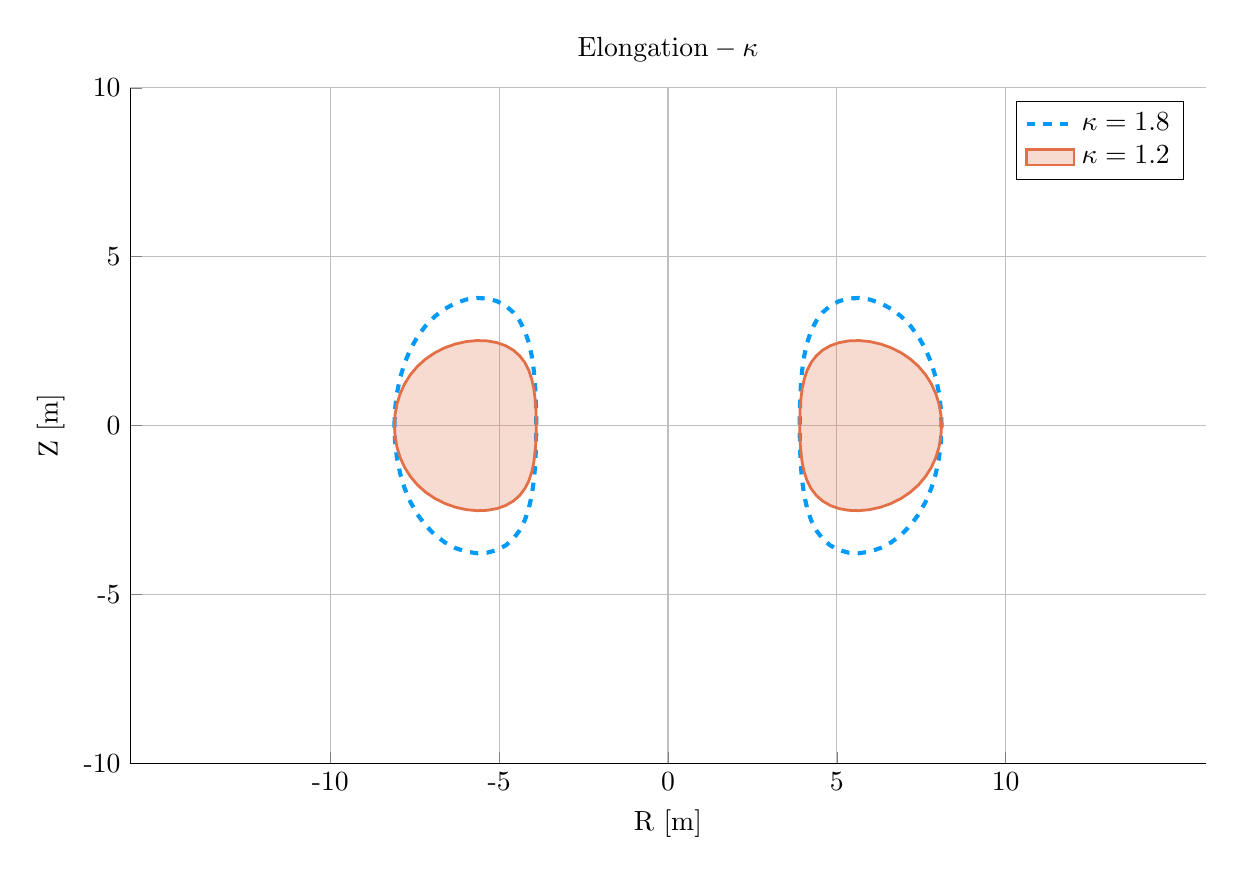
\begin{tikzpicture}[]
\begin{axis}[height = {101.6mm}, axis equal = {true}, ylabel = {Z [m]}, title = {$\textnormal{Elongation} - \kappa$}, xmin = {-10}, xmax = {10}, ymax = {10}, xlabel = {R [m]}, {unbounded coords=jump, scaled x ticks = false, xticklabel style={rotate = 0}, xmajorgrids = true, xtick = {-10.0,-5.0,0.0,5.0,10.0}, xticklabels = {-10,-5,0,5,10}, xtick align = inside, axis lines* = left, scaled y ticks = false, yticklabel style={rotate = 0}, ymajorgrids = true, ytick = {-10.0,-5.0,0.0,5.0,10.0}, yticklabels = {-10,-5,0,5,10}, ytick align = inside, axis lines* = left,     xshift = 0.0mm,
    yshift = 0.0mm,
    axis background/.style={fill={rgb,1:red,1.00000000;green,1.00000000;blue,1.00000000}}
}, ymin = {-10}, width = {152.4mm}]\addplot+ [color = {rgb,1:red,0.00000000;green,0.60560316;blue,0.97868012},
draw opacity=1.0,
line width=1.5,
dashed,mark = none,
mark size = 2.0,
mark options = {
    color = {rgb,1:red,0.00000000;green,0.00000000;blue,0.00000000}, draw opacity = 1.0,
    fill = {rgb,1:red,0.00000000;green,0.60560316;blue,0.97868012}, fill opacity = 1.0,
    line width = 1,
    rotate = 0,
    solid
}]coordinates {
(8.1, 0.0)
(8.081204069972497, 0.48337567116743263)
(8.024684777757766, 0.9588143271779377)
(7.930141280572084, 1.4185092784440338)
(7.797367695668915, 1.854912346574885)
(7.626640572703316, 2.260857805256796)
(7.419158721180681, 2.6296800412811785)
(7.177452352825953, 2.9553230037291525)
(6.905679431512412, 3.232439644160208)
(6.609741255084048, 3.456479714999771)
(6.297174663233395, 3.623764484478577)
(5.976811190071814, 3.7315471413066206)
(5.658229090447864, 3.7780578972385994)
(5.351057127458824, 3.7625330469479685)
(5.06421429716898, 3.685227508047293)
(4.805183334632925, 3.547410635348094)
(4.579415603765742, 3.3513453780899396)
(4.389950548568067, 3.100251122376493)
(4.237306076467235, 2.7982508289446923)
(4.119660690046763, 2.45030333426344)
(4.033308834588962, 2.0621219265758737)
(3.9733333500050683, 1.6400805338643698)
(3.9344084806536994, 1.1911090641292867)
(3.911628010194501, 0.7225796164911881)
(3.9012485454184915, 0.24218543152709598)
(3.9012485454184915, -0.2421854315270951)
(3.911628010194501, -0.7225796164911872)
(3.9344084806536994, -1.1911090641292859)
(3.9733333500050687, -1.640080533864369)
(4.033308834588962, -2.0621219265758732)
(4.119660690046763, -2.450303334263439)
(4.237306076467235, -2.7982508289446915)
(4.389950548568066, -3.1002511223764917)
(4.579415603765742, -3.3513453780899396)
(4.8051833346329245, -3.5474106353480934)
(5.064214297168979, -3.685227508047293)
(5.351057127458825, -3.7625330469479685)
(5.658229090447862, -3.7780578972385994)
(5.976811190071814, -3.731547141306621)
(6.297174663233394, -3.6237644844785772)
(6.609741255084048, -3.456479714999771)
(6.90567943151241, -3.232439644160209)
(7.177452352825952, -2.955323003729153)
(7.419158721180681, -2.629680041281178)
(7.626640572703316, -2.260857805256797)
(7.797367695668915, -1.854912346574885)
(7.930141280572083, -1.4185092784440358)
(8.024684777757766, -0.9588143271779382)
(8.081204069972497, -0.483375671167435)
(8.1, -9.258329801553988e-16)
};
\addlegendentry{$\kappa = 1.8$}
\addplot+ [color = {rgb,1:red,0.00000000;green,0.60560316;blue,0.97868012},
draw opacity=1.0,
line width=1.5,
dashed,mark = none,
mark size = 2.0,
mark options = {
    color = {rgb,1:red,0.00000000;green,0.00000000;blue,0.00000000}, draw opacity = 1.0,
    fill = {rgb,1:red,0.00000000;green,0.60560316;blue,0.97868012}, fill opacity = 1.0,
    line width = 1,
    rotate = 0,
    solid
},forget plot]coordinates {
(-8.1, 0.0)
(-8.081204069972497, 0.48337567116743263)
(-8.024684777757766, 0.9588143271779377)
(-7.930141280572084, 1.4185092784440338)
(-7.797367695668915, 1.854912346574885)
(-7.626640572703316, 2.260857805256796)
(-7.419158721180681, 2.6296800412811785)
(-7.177452352825953, 2.9553230037291525)
(-6.905679431512412, 3.232439644160208)
(-6.609741255084048, 3.456479714999771)
(-6.297174663233395, 3.623764484478577)
(-5.976811190071814, 3.7315471413066206)
(-5.658229090447864, 3.7780578972385994)
(-5.351057127458824, 3.7625330469479685)
(-5.06421429716898, 3.685227508047293)
(-4.805183334632925, 3.547410635348094)
(-4.579415603765742, 3.3513453780899396)
(-4.389950548568067, 3.100251122376493)
(-4.237306076467235, 2.7982508289446923)
(-4.119660690046763, 2.45030333426344)
(-4.033308834588962, 2.0621219265758737)
(-3.9733333500050683, 1.6400805338643698)
(-3.9344084806536994, 1.1911090641292867)
(-3.911628010194501, 0.7225796164911881)
(-3.9012485454184915, 0.24218543152709598)
(-3.9012485454184915, -0.2421854315270951)
(-3.911628010194501, -0.7225796164911872)
(-3.9344084806536994, -1.1911090641292859)
(-3.9733333500050687, -1.640080533864369)
(-4.033308834588962, -2.0621219265758732)
(-4.119660690046763, -2.450303334263439)
(-4.237306076467235, -2.7982508289446915)
(-4.389950548568066, -3.1002511223764917)
(-4.579415603765742, -3.3513453780899396)
(-4.8051833346329245, -3.5474106353480934)
(-5.064214297168979, -3.685227508047293)
(-5.351057127458825, -3.7625330469479685)
(-5.658229090447862, -3.7780578972385994)
(-5.976811190071814, -3.731547141306621)
(-6.297174663233394, -3.6237644844785772)
(-6.609741255084048, -3.456479714999771)
(-6.90567943151241, -3.232439644160209)
(-7.177452352825952, -2.955323003729153)
(-7.419158721180681, -2.629680041281178)
(-7.626640572703316, -2.260857805256797)
(-7.797367695668915, -1.854912346574885)
(-7.930141280572083, -1.4185092784440358)
(-8.024684777757766, -0.9588143271779382)
(-8.081204069972497, -0.483375671167435)
(-8.1, -9.258329801553988e-16)
};
\addplot+ [color = {rgb,1:red,0.88887350;green,0.43564919;blue,0.27812294},
draw opacity=1.0,
line width=1,
solid,mark = none,
mark size = 2.0,
mark options = {
    color = {rgb,1:red,0.00000000;green,0.00000000;blue,0.00000000}, draw opacity = 1.0,
    fill = {rgb,1:red,0.88887350;green,0.43564919;blue,0.27812294}, fill opacity = 1.0,
    line width = 1,
    rotate = 0,
    solid
},fill = {rgb,1:red,0.88887350;green,0.43564919;blue,0.27812294}, fill opacity=0.25,area legend]coordinates {
(8.1, 0.0)
(8.081204069972497, 0.322250447444955)
(8.024684777757766, 0.6392095514519583)
(7.930141280572084, 0.9456728522960225)
(7.797367695668915, 1.2366082310499231)
(7.626640572703316, 1.507238536837864)
(7.419158721180681, 1.7531200275207854)
(7.177452352825953, 1.9702153358194345)
(6.905679431512412, 2.1549597627734713)
(6.609741255084048, 2.304319809999847)
(6.297174663233395, 2.415842989652384)
(5.976811190071814, 2.487698094204414)
(5.658229090447864, 2.518705264825733)
(5.351057127458824, 2.508355364631979)
(5.06421429716898, 2.456818338698195)
(4.805183334632925, 2.364940423565396)
(4.579415603765742, 2.2342302520599597)
(4.389950548568067, 2.0668340815843287)
(4.237306076467235, 1.8655005526297948)
(4.119660690046763, 1.6335355561756264)
(4.033308834588962, 1.3747479510505825)
(3.9733333500050683, 1.0933870225762463)
(3.9344084806536994, 0.7940727094195245)
(3.911628010194501, 0.48171974432745873)
(3.9012485454184915, 0.16145695435139729)
(3.9012485454184915, -0.1614569543513967)
(3.911628010194501, -0.48171974432745807)
(3.9344084806536994, -0.7940727094195238)
(3.9733333500050687, -1.0933870225762459)
(4.033308834588962, -1.3747479510505818)
(4.119660690046763, -1.633535556175626)
(4.237306076467235, -1.8655005526297943)
(4.389950548568066, -2.066834081584328)
(4.579415603765742, -2.2342302520599593)
(4.8051833346329245, -2.3649404235653955)
(5.064214297168979, -2.456818338698195)
(5.351057127458825, -2.508355364631979)
(5.658229090447862, -2.518705264825733)
(5.976811190071814, -2.487698094204414)
(6.297174663233394, -2.415842989652385)
(6.609741255084048, -2.304319809999847)
(6.90567943151241, -2.1549597627734722)
(7.177452352825952, -1.9702153358194348)
(7.419158721180681, -1.7531200275207852)
(7.626640572703316, -1.5072385368378645)
(7.797367695668915, -1.2366082310499231)
(7.930141280572083, -0.9456728522960237)
(8.024684777757766, -0.6392095514519588)
(8.081204069972497, -0.3222504474449567)
(8.1, -6.172219867702659e-16)
};
\addlegendentry{$\kappa = 1.2$}
\addplot+ [color = {rgb,1:red,0.88887350;green,0.43564919;blue,0.27812294},
draw opacity=1.0,
line width=1,
solid,mark = none,
mark size = 2.0,
mark options = {
    color = {rgb,1:red,0.00000000;green,0.00000000;blue,0.00000000}, draw opacity = 1.0,
    fill = {rgb,1:red,0.88887350;green,0.43564919;blue,0.27812294}, fill opacity = 1.0,
    line width = 1,
    rotate = 0,
    solid
},fill = {rgb,1:red,0.88887350;green,0.43564919;blue,0.27812294}, fill opacity=0.25,forget plot]coordinates {
(-8.1, 0.0)
(-8.081204069972497, 0.322250447444955)
(-8.024684777757766, 0.6392095514519583)
(-7.930141280572084, 0.9456728522960225)
(-7.797367695668915, 1.2366082310499231)
(-7.626640572703316, 1.507238536837864)
(-7.419158721180681, 1.7531200275207854)
(-7.177452352825953, 1.9702153358194345)
(-6.905679431512412, 2.1549597627734713)
(-6.609741255084048, 2.304319809999847)
(-6.297174663233395, 2.415842989652384)
(-5.976811190071814, 2.487698094204414)
(-5.658229090447864, 2.518705264825733)
(-5.351057127458824, 2.508355364631979)
(-5.06421429716898, 2.456818338698195)
(-4.805183334632925, 2.364940423565396)
(-4.579415603765742, 2.2342302520599597)
(-4.389950548568067, 2.0668340815843287)
(-4.237306076467235, 1.8655005526297948)
(-4.119660690046763, 1.6335355561756264)
(-4.033308834588962, 1.3747479510505825)
(-3.9733333500050683, 1.0933870225762463)
(-3.9344084806536994, 0.7940727094195245)
(-3.911628010194501, 0.48171974432745873)
(-3.9012485454184915, 0.16145695435139729)
(-3.9012485454184915, -0.1614569543513967)
(-3.911628010194501, -0.48171974432745807)
(-3.9344084806536994, -0.7940727094195238)
(-3.9733333500050687, -1.0933870225762459)
(-4.033308834588962, -1.3747479510505818)
(-4.119660690046763, -1.633535556175626)
(-4.237306076467235, -1.8655005526297943)
(-4.389950548568066, -2.066834081584328)
(-4.579415603765742, -2.2342302520599593)
(-4.8051833346329245, -2.3649404235653955)
(-5.064214297168979, -2.456818338698195)
(-5.351057127458825, -2.508355364631979)
(-5.658229090447862, -2.518705264825733)
(-5.976811190071814, -2.487698094204414)
(-6.297174663233394, -2.415842989652385)
(-6.609741255084048, -2.304319809999847)
(-6.90567943151241, -2.1549597627734722)
(-7.177452352825952, -1.9702153358194348)
(-7.419158721180681, -1.7531200275207852)
(-7.626640572703316, -1.5072385368378645)
(-7.797367695668915, -1.2366082310499231)
(-7.930141280572083, -0.9456728522960237)
(-8.024684777757766, -0.6392095514519588)
(-8.081204069972497, -0.3222504474449567)
(-8.1, -6.172219867702659e-16)
};
\end{axis}

\end{tikzpicture}

		\end{adjustbox}
        \caption{$\kappa$}
    \end{subfigure}
    \hfill
    \begin{subfigure}[t]{0.45\textwidth}
        \centering
		\begin{adjustbox}{width=\textwidth}
			\Large
			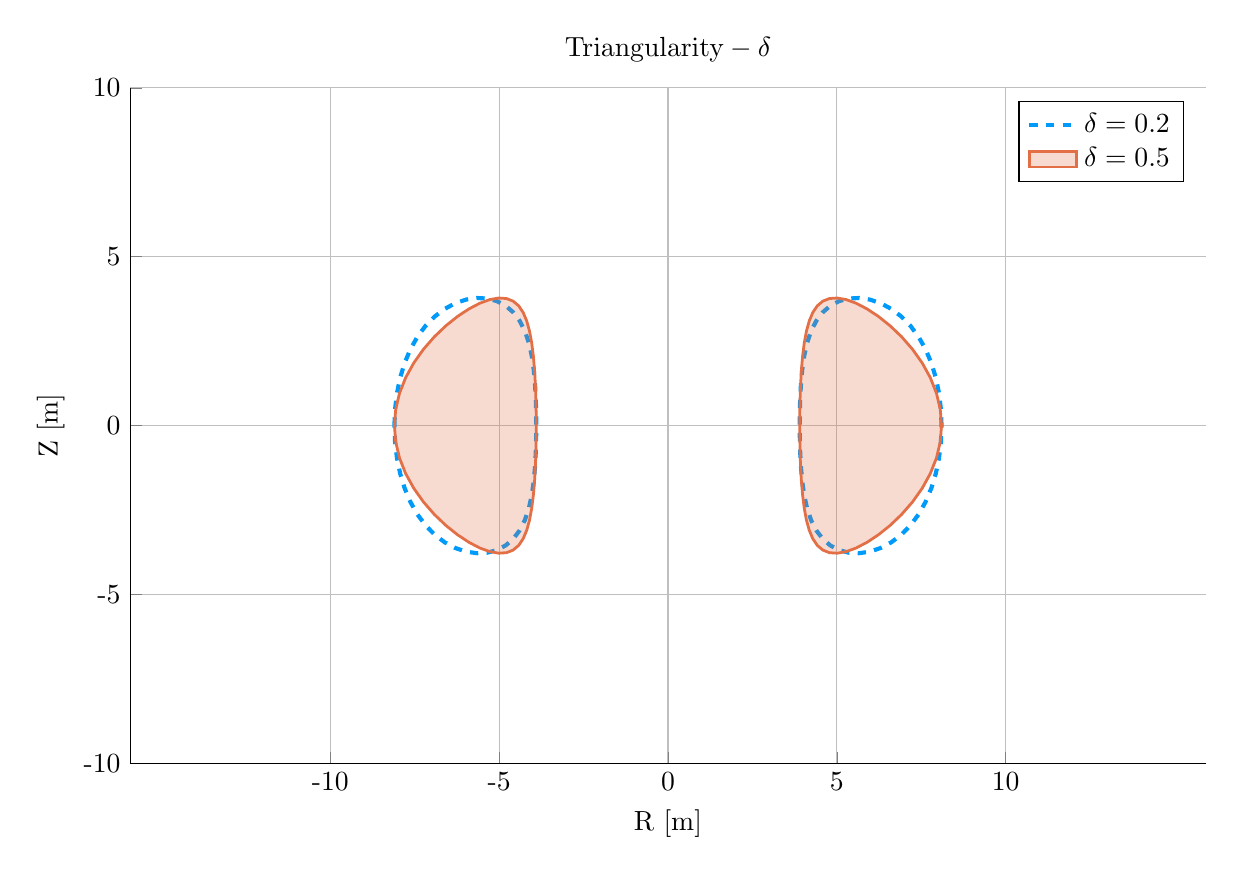
\begin{tikzpicture}[]
\begin{axis}[height = {101.6mm}, axis equal = {true}, ylabel = {Z [m]}, title = {$\textnormal{Triangularity} - \delta$}, xmin = {-10}, xmax = {10}, ymax = {10}, xlabel = {R [m]}, {unbounded coords=jump, scaled x ticks = false, xticklabel style={rotate = 0}, xmajorgrids = true, xtick = {-10.0,-5.0,0.0,5.0,10.0}, xticklabels = {-10,-5,0,5,10}, xtick align = inside, axis lines* = left, scaled y ticks = false, yticklabel style={rotate = 0}, ymajorgrids = true, ytick = {-10.0,-5.0,0.0,5.0,10.0}, yticklabels = {-10,-5,0,5,10}, ytick align = inside, axis lines* = left,     xshift = 0.0mm,
    yshift = 0.0mm,
    axis background/.style={fill={rgb,1:red,1.00000000;green,1.00000000;blue,1.00000000}}
}, ymin = {-10}, width = {152.4mm}]\addplot+ [color = {rgb,1:red,0.00000000;green,0.60560316;blue,0.97868012},
draw opacity=1.0,
line width=1.5,
dashed,mark = none,
mark size = 2.0,
mark options = {
    color = {rgb,1:red,0.00000000;green,0.00000000;blue,0.00000000}, draw opacity = 1.0,
    fill = {rgb,1:red,0.00000000;green,0.60560316;blue,0.97868012}, fill opacity = 1.0,
    line width = 1,
    rotate = 0,
    solid
}]coordinates {
(8.1, 0.0)
(8.081204069972497, 0.48337567116743263)
(8.024684777757766, 0.9588143271779377)
(7.930141280572084, 1.4185092784440338)
(7.797367695668915, 1.854912346574885)
(7.626640572703316, 2.260857805256796)
(7.419158721180681, 2.6296800412811785)
(7.177452352825953, 2.9553230037291525)
(6.905679431512412, 3.232439644160208)
(6.609741255084048, 3.456479714999771)
(6.297174663233395, 3.623764484478577)
(5.976811190071814, 3.7315471413066206)
(5.658229090447864, 3.7780578972385994)
(5.351057127458824, 3.7625330469479685)
(5.06421429716898, 3.685227508047293)
(4.805183334632925, 3.547410635348094)
(4.579415603765742, 3.3513453780899396)
(4.389950548568067, 3.100251122376493)
(4.237306076467235, 2.7982508289446923)
(4.119660690046763, 2.45030333426344)
(4.033308834588962, 2.0621219265758737)
(3.9733333500050683, 1.6400805338643698)
(3.9344084806536994, 1.1911090641292867)
(3.911628010194501, 0.7225796164911881)
(3.9012485454184915, 0.24218543152709598)
(3.9012485454184915, -0.2421854315270951)
(3.911628010194501, -0.7225796164911872)
(3.9344084806536994, -1.1911090641292859)
(3.9733333500050687, -1.640080533864369)
(4.033308834588962, -2.0621219265758732)
(4.119660690046763, -2.450303334263439)
(4.237306076467235, -2.7982508289446915)
(4.389950548568066, -3.1002511223764917)
(4.579415603765742, -3.3513453780899396)
(4.8051833346329245, -3.5474106353480934)
(5.064214297168979, -3.685227508047293)
(5.351057127458825, -3.7625330469479685)
(5.658229090447862, -3.7780578972385994)
(5.976811190071814, -3.731547141306621)
(6.297174663233394, -3.6237644844785772)
(6.609741255084048, -3.456479714999771)
(6.90567943151241, -3.232439644160209)
(7.177452352825952, -2.955323003729153)
(7.419158721180681, -2.629680041281178)
(7.626640572703316, -2.260857805256797)
(7.797367695668915, -1.854912346574885)
(7.930141280572083, -1.4185092784440358)
(8.024684777757766, -0.9588143271779382)
(8.081204069972497, -0.483375671167435)
(8.1, -9.258329801553988e-16)
};
\addlegendentry{$\delta = 0.2$}
\addplot+ [color = {rgb,1:red,0.00000000;green,0.60560316;blue,0.97868012},
draw opacity=1.0,
line width=1.5,
dashed,mark = none,
mark size = 2.0,
mark options = {
    color = {rgb,1:red,0.00000000;green,0.00000000;blue,0.00000000}, draw opacity = 1.0,
    fill = {rgb,1:red,0.00000000;green,0.60560316;blue,0.97868012}, fill opacity = 1.0,
    line width = 1,
    rotate = 0,
    solid
},forget plot]coordinates {
(-8.1, 0.0)
(-8.081204069972497, 0.48337567116743263)
(-8.024684777757766, 0.9588143271779377)
(-7.930141280572084, 1.4185092784440338)
(-7.797367695668915, 1.854912346574885)
(-7.626640572703316, 2.260857805256796)
(-7.419158721180681, 2.6296800412811785)
(-7.177452352825953, 2.9553230037291525)
(-6.905679431512412, 3.232439644160208)
(-6.609741255084048, 3.456479714999771)
(-6.297174663233395, 3.623764484478577)
(-5.976811190071814, 3.7315471413066206)
(-5.658229090447864, 3.7780578972385994)
(-5.351057127458824, 3.7625330469479685)
(-5.06421429716898, 3.685227508047293)
(-4.805183334632925, 3.547410635348094)
(-4.579415603765742, 3.3513453780899396)
(-4.389950548568067, 3.100251122376493)
(-4.237306076467235, 2.7982508289446923)
(-4.119660690046763, 2.45030333426344)
(-4.033308834588962, 2.0621219265758737)
(-3.9733333500050683, 1.6400805338643698)
(-3.9344084806536994, 1.1911090641292867)
(-3.911628010194501, 0.7225796164911881)
(-3.9012485454184915, 0.24218543152709598)
(-3.9012485454184915, -0.2421854315270951)
(-3.911628010194501, -0.7225796164911872)
(-3.9344084806536994, -1.1911090641292859)
(-3.9733333500050687, -1.640080533864369)
(-4.033308834588962, -2.0621219265758732)
(-4.119660690046763, -2.450303334263439)
(-4.237306076467235, -2.7982508289446915)
(-4.389950548568066, -3.1002511223764917)
(-4.579415603765742, -3.3513453780899396)
(-4.8051833346329245, -3.5474106353480934)
(-5.064214297168979, -3.685227508047293)
(-5.351057127458825, -3.7625330469479685)
(-5.658229090447862, -3.7780578972385994)
(-5.976811190071814, -3.731547141306621)
(-6.297174663233394, -3.6237644844785772)
(-6.609741255084048, -3.456479714999771)
(-6.90567943151241, -3.232439644160209)
(-7.177452352825952, -2.955323003729153)
(-7.419158721180681, -2.629680041281178)
(-7.626640572703316, -2.260857805256797)
(-7.797367695668915, -1.854912346574885)
(-7.930141280572083, -1.4185092784440358)
(-8.024684777757766, -0.9588143271779382)
(-8.081204069972497, -0.483375671167435)
(-8.1, -9.258329801553988e-16)
};
\addplot+ [color = {rgb,1:red,0.88887350;green,0.43564919;blue,0.27812294},
draw opacity=1.0,
line width=1,
solid,mark = none,
mark size = 2.0,
mark options = {
    color = {rgb,1:red,0.00000000;green,0.00000000;blue,0.00000000}, draw opacity = 1.0,
    fill = {rgb,1:red,0.88887350;green,0.43564919;blue,0.27812294}, fill opacity = 1.0,
    line width = 1,
    rotate = 0,
    solid
},fill = {rgb,1:red,0.88887350;green,0.43564919;blue,0.27812294}, fill opacity=0.25,area legend]coordinates {
(8.1, 0.0)
(8.061757255413621, 0.48337567116743263)
(7.949058187688645, 0.9588143271779377)
(7.76782009445037, 1.4185092784440338)
(7.5273561623601815, 1.854912346574885)
(7.239613973335666, 2.260857805256796)
(6.918225433609141, 2.6296800412811785)
(6.577466753393508, 2.9553230037291525)
(6.231233080250507, 3.232439644160208)
(5.8921259319088515, 3.456479714999771)
(5.57073386435538, 3.623764484478577)
(5.275160475821737, 3.7315471413066206)
(5.010822575438551, 3.7780578972385994)
(4.780509358726627, 3.7625330469479685)
(4.584664892127046, 3.685227508047293)
(4.421834642060505, 3.547410635348094)
(4.289204609388892, 3.3513453780899396)
(4.1831598532589656, 3.100251122376493)
(4.099797305222337, 2.7982508289446923)
(4.035343895299359, 2.45030333426344)
(3.9864521823619747, 2.0621219265758737)
(3.950368354479447, 1.6400805338643698)
(3.9249880475776253, 1.1911090641292867)
(3.908830826940035, 0.7225796164911881)
(3.90097224453103, 0.24218543152709598)
(3.90097224453103, -0.2421854315270951)
(3.908830826940035, -0.7225796164911872)
(3.9249880475776253, -1.1911090641292859)
(3.9503683544794472, -1.640080533864369)
(3.986452182361975, -2.0621219265758732)
(4.035343895299359, -2.450303334263439)
(4.099797305222337, -2.7982508289446915)
(4.1831598532589656, -3.1002511223764917)
(4.289204609388891, -3.3513453780899396)
(4.421834642060504, -3.5474106353480934)
(4.584664892127046, -3.685227508047293)
(4.780509358726627, -3.7625330469479685)
(5.01082257543855, -3.7780578972385994)
(5.275160475821737, -3.731547141306621)
(5.570733864355378, -3.6237644844785772)
(5.8921259319088515, -3.456479714999771)
(6.231233080250505, -3.232439644160209)
(6.577466753393507, -2.955323003729153)
(6.918225433609141, -2.629680041281178)
(7.239613973335665, -2.260857805256797)
(7.5273561623601815, -1.854912346574885)
(7.767820094450369, -1.4185092784440358)
(7.949058187688645, -0.9588143271779382)
(8.061757255413621, -0.483375671167435)
(8.1, -9.258329801553988e-16)
};
\addlegendentry{$\delta = 0.5$}
\addplot+ [color = {rgb,1:red,0.88887350;green,0.43564919;blue,0.27812294},
draw opacity=1.0,
line width=1,
solid,mark = none,
mark size = 2.0,
mark options = {
    color = {rgb,1:red,0.00000000;green,0.00000000;blue,0.00000000}, draw opacity = 1.0,
    fill = {rgb,1:red,0.88887350;green,0.43564919;blue,0.27812294}, fill opacity = 1.0,
    line width = 1,
    rotate = 0,
    solid
},fill = {rgb,1:red,0.88887350;green,0.43564919;blue,0.27812294}, fill opacity=0.25,forget plot]coordinates {
(-8.1, 0.0)
(-8.061757255413621, 0.48337567116743263)
(-7.949058187688645, 0.9588143271779377)
(-7.76782009445037, 1.4185092784440338)
(-7.5273561623601815, 1.854912346574885)
(-7.239613973335666, 2.260857805256796)
(-6.918225433609141, 2.6296800412811785)
(-6.577466753393508, 2.9553230037291525)
(-6.231233080250507, 3.232439644160208)
(-5.8921259319088515, 3.456479714999771)
(-5.57073386435538, 3.623764484478577)
(-5.275160475821737, 3.7315471413066206)
(-5.010822575438551, 3.7780578972385994)
(-4.780509358726627, 3.7625330469479685)
(-4.584664892127046, 3.685227508047293)
(-4.421834642060505, 3.547410635348094)
(-4.289204609388892, 3.3513453780899396)
(-4.1831598532589656, 3.100251122376493)
(-4.099797305222337, 2.7982508289446923)
(-4.035343895299359, 2.45030333426344)
(-3.9864521823619747, 2.0621219265758737)
(-3.950368354479447, 1.6400805338643698)
(-3.9249880475776253, 1.1911090641292867)
(-3.908830826940035, 0.7225796164911881)
(-3.90097224453103, 0.24218543152709598)
(-3.90097224453103, -0.2421854315270951)
(-3.908830826940035, -0.7225796164911872)
(-3.9249880475776253, -1.1911090641292859)
(-3.9503683544794472, -1.640080533864369)
(-3.986452182361975, -2.0621219265758732)
(-4.035343895299359, -2.450303334263439)
(-4.099797305222337, -2.7982508289446915)
(-4.1831598532589656, -3.1002511223764917)
(-4.289204609388891, -3.3513453780899396)
(-4.421834642060504, -3.5474106353480934)
(-4.584664892127046, -3.685227508047293)
(-4.780509358726627, -3.7625330469479685)
(-5.01082257543855, -3.7780578972385994)
(-5.275160475821737, -3.731547141306621)
(-5.570733864355378, -3.6237644844785772)
(-5.8921259319088515, -3.456479714999771)
(-6.231233080250505, -3.232439644160209)
(-6.577466753393507, -2.955323003729153)
(-6.918225433609141, -2.629680041281178)
(-7.239613973335665, -2.260857805256797)
(-7.5273561623601815, -1.854912346574885)
(-7.767820094450369, -1.4185092784440358)
(-7.949058187688645, -0.9588143271779382)
(-8.061757255413621, -0.483375671167435)
(-8.1, -9.258329801553988e-16)
};
\end{axis}

\end{tikzpicture}

		\end{adjustbox}
        \caption{$\delta$}
    \end{subfigure}
    \hfill \hfill ~\\ ~\\ ~\\
    \begin{subfigure}[t]{0.6\textwidth}
        \centering
		\begin{adjustbox}{width=\textwidth}
			\large
			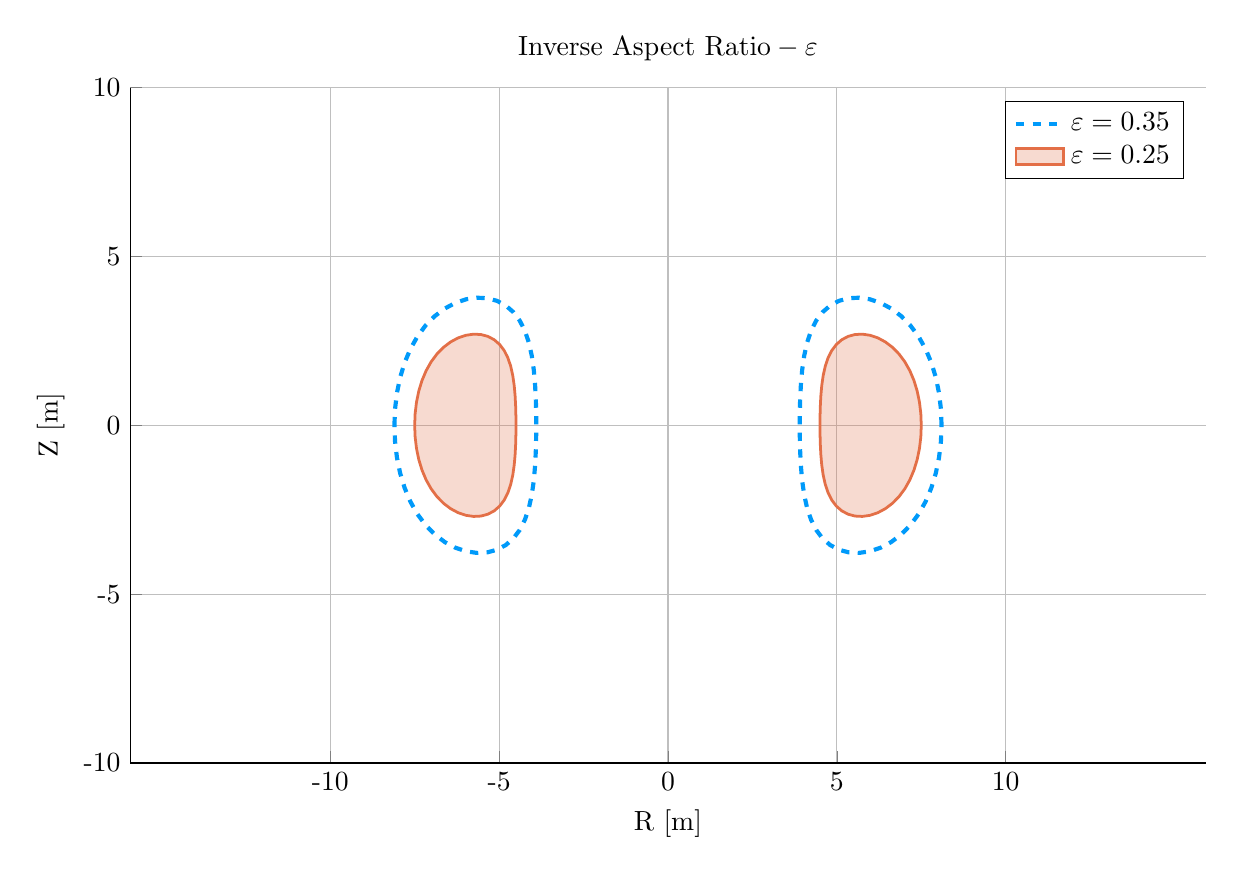
\begin{tikzpicture}[]
\begin{axis}[height = {101.6mm}, axis equal = {true}, ylabel = {Z [m]}, title = {$\textnormal{Inverse Aspect Ratio} - \varepsilon$}, xmin = {-10}, xmax = {10}, ymax = {10}, xlabel = {R [m]}, {unbounded coords=jump, scaled x ticks = false, xticklabel style={rotate = 0}, xmajorgrids = true, xtick = {-10.0,-5.0,0.0,5.0,10.0}, xticklabels = {-10,-5,0,5,10}, xtick align = inside, axis lines* = left, scaled y ticks = false, yticklabel style={rotate = 0}, ymajorgrids = true, ytick = {-10.0,-5.0,0.0,5.0,10.0}, yticklabels = {-10,-5,0,5,10}, ytick align = inside, axis lines* = left,     xshift = 0.0mm,
    yshift = 0.0mm,
    axis background/.style={fill={rgb,1:red,1.00000000;green,1.00000000;blue,1.00000000}}
}, ymin = {-10}, width = {152.4mm}]\addplot+ [color = {rgb,1:red,0.00000000;green,0.60560316;blue,0.97868012},
draw opacity=1.0,
line width=1.5,
dashed,mark = none,
mark size = 2.0,
mark options = {
    color = {rgb,1:red,0.00000000;green,0.00000000;blue,0.00000000}, draw opacity = 1.0,
    fill = {rgb,1:red,0.00000000;green,0.60560316;blue,0.97868012}, fill opacity = 1.0,
    line width = 1,
    rotate = 0,
    solid
}]coordinates {
(8.1, 0.0)
(8.081204069972497, 0.48337567116743263)
(8.024684777757766, 0.9588143271779377)
(7.930141280572084, 1.4185092784440338)
(7.797367695668915, 1.854912346574885)
(7.626640572703316, 2.260857805256796)
(7.419158721180681, 2.6296800412811785)
(7.177452352825953, 2.9553230037291525)
(6.905679431512412, 3.232439644160208)
(6.609741255084048, 3.456479714999771)
(6.297174663233395, 3.623764484478577)
(5.976811190071814, 3.7315471413066206)
(5.658229090447864, 3.7780578972385994)
(5.351057127458824, 3.7625330469479685)
(5.06421429716898, 3.685227508047293)
(4.805183334632925, 3.547410635348094)
(4.579415603765742, 3.3513453780899396)
(4.389950548568067, 3.100251122376493)
(4.237306076467235, 2.7982508289446923)
(4.119660690046763, 2.45030333426344)
(4.033308834588962, 2.0621219265758737)
(3.9733333500050683, 1.6400805338643698)
(3.9344084806536994, 1.1911090641292867)
(3.911628010194501, 0.7225796164911881)
(3.9012485454184915, 0.24218543152709598)
(3.9012485454184915, -0.2421854315270951)
(3.911628010194501, -0.7225796164911872)
(3.9344084806536994, -1.1911090641292859)
(3.9733333500050687, -1.640080533864369)
(4.033308834588962, -2.0621219265758732)
(4.119660690046763, -2.450303334263439)
(4.237306076467235, -2.7982508289446915)
(4.389950548568066, -3.1002511223764917)
(4.579415603765742, -3.3513453780899396)
(4.8051833346329245, -3.5474106353480934)
(5.064214297168979, -3.685227508047293)
(5.351057127458825, -3.7625330469479685)
(5.658229090447862, -3.7780578972385994)
(5.976811190071814, -3.731547141306621)
(6.297174663233394, -3.6237644844785772)
(6.609741255084048, -3.456479714999771)
(6.90567943151241, -3.232439644160209)
(7.177452352825952, -2.955323003729153)
(7.419158721180681, -2.629680041281178)
(7.626640572703316, -2.260857805256797)
(7.797367695668915, -1.854912346574885)
(7.930141280572083, -1.4185092784440358)
(8.024684777757766, -0.9588143271779382)
(8.081204069972497, -0.483375671167435)
(8.1, -9.258329801553988e-16)
};
\addlegendentry{$\varepsilon = 0.35$}
\addplot+ [color = {rgb,1:red,0.00000000;green,0.60560316;blue,0.97868012},
draw opacity=1.0,
line width=1.5,
dashed,mark = none,
mark size = 2.0,
mark options = {
    color = {rgb,1:red,0.00000000;green,0.00000000;blue,0.00000000}, draw opacity = 1.0,
    fill = {rgb,1:red,0.00000000;green,0.60560316;blue,0.97868012}, fill opacity = 1.0,
    line width = 1,
    rotate = 0,
    solid
},forget plot]coordinates {
(-8.1, 0.0)
(-8.081204069972497, 0.48337567116743263)
(-8.024684777757766, 0.9588143271779377)
(-7.930141280572084, 1.4185092784440338)
(-7.797367695668915, 1.854912346574885)
(-7.626640572703316, 2.260857805256796)
(-7.419158721180681, 2.6296800412811785)
(-7.177452352825953, 2.9553230037291525)
(-6.905679431512412, 3.232439644160208)
(-6.609741255084048, 3.456479714999771)
(-6.297174663233395, 3.623764484478577)
(-5.976811190071814, 3.7315471413066206)
(-5.658229090447864, 3.7780578972385994)
(-5.351057127458824, 3.7625330469479685)
(-5.06421429716898, 3.685227508047293)
(-4.805183334632925, 3.547410635348094)
(-4.579415603765742, 3.3513453780899396)
(-4.389950548568067, 3.100251122376493)
(-4.237306076467235, 2.7982508289446923)
(-4.119660690046763, 2.45030333426344)
(-4.033308834588962, 2.0621219265758737)
(-3.9733333500050683, 1.6400805338643698)
(-3.9344084806536994, 1.1911090641292867)
(-3.911628010194501, 0.7225796164911881)
(-3.9012485454184915, 0.24218543152709598)
(-3.9012485454184915, -0.2421854315270951)
(-3.911628010194501, -0.7225796164911872)
(-3.9344084806536994, -1.1911090641292859)
(-3.9733333500050687, -1.640080533864369)
(-4.033308834588962, -2.0621219265758732)
(-4.119660690046763, -2.450303334263439)
(-4.237306076467235, -2.7982508289446915)
(-4.389950548568066, -3.1002511223764917)
(-4.579415603765742, -3.3513453780899396)
(-4.8051833346329245, -3.5474106353480934)
(-5.064214297168979, -3.685227508047293)
(-5.351057127458825, -3.7625330469479685)
(-5.658229090447862, -3.7780578972385994)
(-5.976811190071814, -3.731547141306621)
(-6.297174663233394, -3.6237644844785772)
(-6.609741255084048, -3.456479714999771)
(-6.90567943151241, -3.232439644160209)
(-7.177452352825952, -2.955323003729153)
(-7.419158721180681, -2.629680041281178)
(-7.626640572703316, -2.260857805256797)
(-7.797367695668915, -1.854912346574885)
(-7.930141280572083, -1.4185092784440358)
(-8.024684777757766, -0.9588143271779382)
(-8.081204069972497, -0.483375671167435)
(-8.1, -9.258329801553988e-16)
};
\addplot+ [color = {rgb,1:red,0.88887350;green,0.43564919;blue,0.27812294},
draw opacity=1.0,
line width=1,
solid,mark = none,
mark size = 2.0,
mark options = {
    color = {rgb,1:red,0.00000000;green,0.00000000;blue,0.00000000}, draw opacity = 1.0,
    fill = {rgb,1:red,0.88887350;green,0.43564919;blue,0.27812294}, fill opacity = 1.0,
    line width = 1,
    rotate = 0,
    solid
},fill = {rgb,1:red,0.88887350;green,0.43564919;blue,0.27812294}, fill opacity=0.25,area legend]coordinates {
(7.5, 0.0)
(7.486574335694641, 0.34526833654816624)
(7.446203412684119, 0.6848673765556699)
(7.378672343265774, 1.0132209131743102)
(7.283834068334939, 1.3249373904106323)
(7.161886123359512, 1.6148984323262832)
(7.013684800843344, 1.8783428866294134)
(6.841037394875681, 2.1109450026636805)
(6.646913879651723, 2.3088854601144346)
(6.435529467917177, 2.468914082142694)
(6.212267616595282, 2.588403203198984)
(5.98343656433701, 2.6653908152190153)
(5.755877921748474, 2.6986127837418574)
(5.536469376756303, 2.687523604962835)
(5.331581640834985, 2.632305362890924)
(5.146559524737804, 2.533864739534353)
(4.985296859832673, 2.3938181272071004)
(4.84996467754862, 2.214465087411781)
(4.74093291176231, 1.998750592103352)
(4.6569004928905455, 1.7502166673310287)
(4.595220596134973, 1.4729442332684815)
(4.552380964289334, 1.1714860956174071)
(4.524577486181213, 0.8507921886637764)
(4.508305721567501, 0.5161282974937058)
(4.500891818156065, 0.17298959394792573)
(4.500891818156065, -0.1729895939479251)
(4.508305721567501, -0.5161282974937051)
(4.524577486181213, -0.8507921886637757)
(4.552380964289334, -1.1714860956174067)
(4.595220596134973, -1.472944233268481)
(4.656900492890545, -1.7502166673310282)
(4.74093291176231, -1.9987505921033515)
(4.849964677548619, -2.21446508741178)
(4.985296859832673, -2.3938181272071004)
(5.146559524737803, -2.5338647395343528)
(5.331581640834985, -2.632305362890924)
(5.536469376756303, -2.687523604962835)
(5.755877921748473, -2.6986127837418574)
(5.98343656433701, -2.6653908152190153)
(6.212267616595281, -2.5884032031989843)
(6.435529467917177, -2.468914082142694)
(6.646913879651722, -2.3088854601144355)
(6.841037394875681, -2.110945002663681)
(7.013684800843344, -1.878342886629413)
(7.161886123359511, -1.6148984323262838)
(7.283834068334939, -1.3249373904106323)
(7.378672343265773, -1.0132209131743115)
(7.446203412684119, -0.6848673765556703)
(7.486574335694641, -0.3452683365481679)
(7.5, -6.613092715395707e-16)
};
\addlegendentry{$\varepsilon = 0.25$}
\addplot+ [color = {rgb,1:red,0.88887350;green,0.43564919;blue,0.27812294},
draw opacity=1.0,
line width=1,
solid,mark = none,
mark size = 2.0,
mark options = {
    color = {rgb,1:red,0.00000000;green,0.00000000;blue,0.00000000}, draw opacity = 1.0,
    fill = {rgb,1:red,0.88887350;green,0.43564919;blue,0.27812294}, fill opacity = 1.0,
    line width = 1,
    rotate = 0,
    solid
},fill = {rgb,1:red,0.88887350;green,0.43564919;blue,0.27812294}, fill opacity=0.25,forget plot]coordinates {
(-7.5, 0.0)
(-7.486574335694641, 0.34526833654816624)
(-7.446203412684119, 0.6848673765556699)
(-7.378672343265774, 1.0132209131743102)
(-7.283834068334939, 1.3249373904106323)
(-7.161886123359512, 1.6148984323262832)
(-7.013684800843344, 1.8783428866294134)
(-6.841037394875681, 2.1109450026636805)
(-6.646913879651723, 2.3088854601144346)
(-6.435529467917177, 2.468914082142694)
(-6.212267616595282, 2.588403203198984)
(-5.98343656433701, 2.6653908152190153)
(-5.755877921748474, 2.6986127837418574)
(-5.536469376756303, 2.687523604962835)
(-5.331581640834985, 2.632305362890924)
(-5.146559524737804, 2.533864739534353)
(-4.985296859832673, 2.3938181272071004)
(-4.84996467754862, 2.214465087411781)
(-4.74093291176231, 1.998750592103352)
(-4.6569004928905455, 1.7502166673310287)
(-4.595220596134973, 1.4729442332684815)
(-4.552380964289334, 1.1714860956174071)
(-4.524577486181213, 0.8507921886637764)
(-4.508305721567501, 0.5161282974937058)
(-4.500891818156065, 0.17298959394792573)
(-4.500891818156065, -0.1729895939479251)
(-4.508305721567501, -0.5161282974937051)
(-4.524577486181213, -0.8507921886637757)
(-4.552380964289334, -1.1714860956174067)
(-4.595220596134973, -1.472944233268481)
(-4.656900492890545, -1.7502166673310282)
(-4.74093291176231, -1.9987505921033515)
(-4.849964677548619, -2.21446508741178)
(-4.985296859832673, -2.3938181272071004)
(-5.146559524737803, -2.5338647395343528)
(-5.331581640834985, -2.632305362890924)
(-5.536469376756303, -2.687523604962835)
(-5.755877921748473, -2.6986127837418574)
(-5.98343656433701, -2.6653908152190153)
(-6.212267616595281, -2.5884032031989843)
(-6.435529467917177, -2.468914082142694)
(-6.646913879651722, -2.3088854601144355)
(-6.841037394875681, -2.110945002663681)
(-7.013684800843344, -1.878342886629413)
(-7.161886123359511, -1.6148984323262838)
(-7.283834068334939, -1.3249373904106323)
(-7.378672343265773, -1.0132209131743115)
(-7.446203412684119, -0.6848673765556703)
(-7.486574335694641, -0.3452683365481679)
(-7.5, -6.613092715395707e-16)
};
\end{axis}

\end{tikzpicture}

		\end{adjustbox}
        \caption{$\epsilon$}
    \end{subfigure} ~\\ ~\\
    \caption{Geometric Parameters} ~\\
    \small These three geometric parameters allow the toroidal cross-sections to scale radially, stretch vertically, and become more triangular -- thus improving upon simple circular slices.
    \label{fig:geometry}
\end{figure*}

These geometric factors allow the volumetric and surface integrals governing fusion power and bootstrap current to be condensed to simple radial ones -- see \cref{eq:qs,eq:qv}. The only remaining step is to define the radial profiles for: the density, temperature, and current of a plasma.

\subsection{Prescribing Plasma Profiles}

The first step in defining radial profiles is realizing that all three quantities are \replaced{essentially parabolas}{basically parabolas} -- i.e.\ the temperature, density and current \added{density}, shown in \cref{fig:profiles}, are peaked at some radius (usually the center) and then decay to zero somewhere before the walls of the tokamak enclosure.

\added{Although not self-consistent, these profiles do capture enough of the physics to approximate relevant phenomenon, such as transport and fusion power.\cite{process_guide}}

\begin{figure*}
	\label{fig:profiles}
    \centering
    \hfill 
    \begin{subfigure}[t]{0.45\textwidth}
        \centering
		\begin{adjustbox}{width=\textwidth}
			\Large
			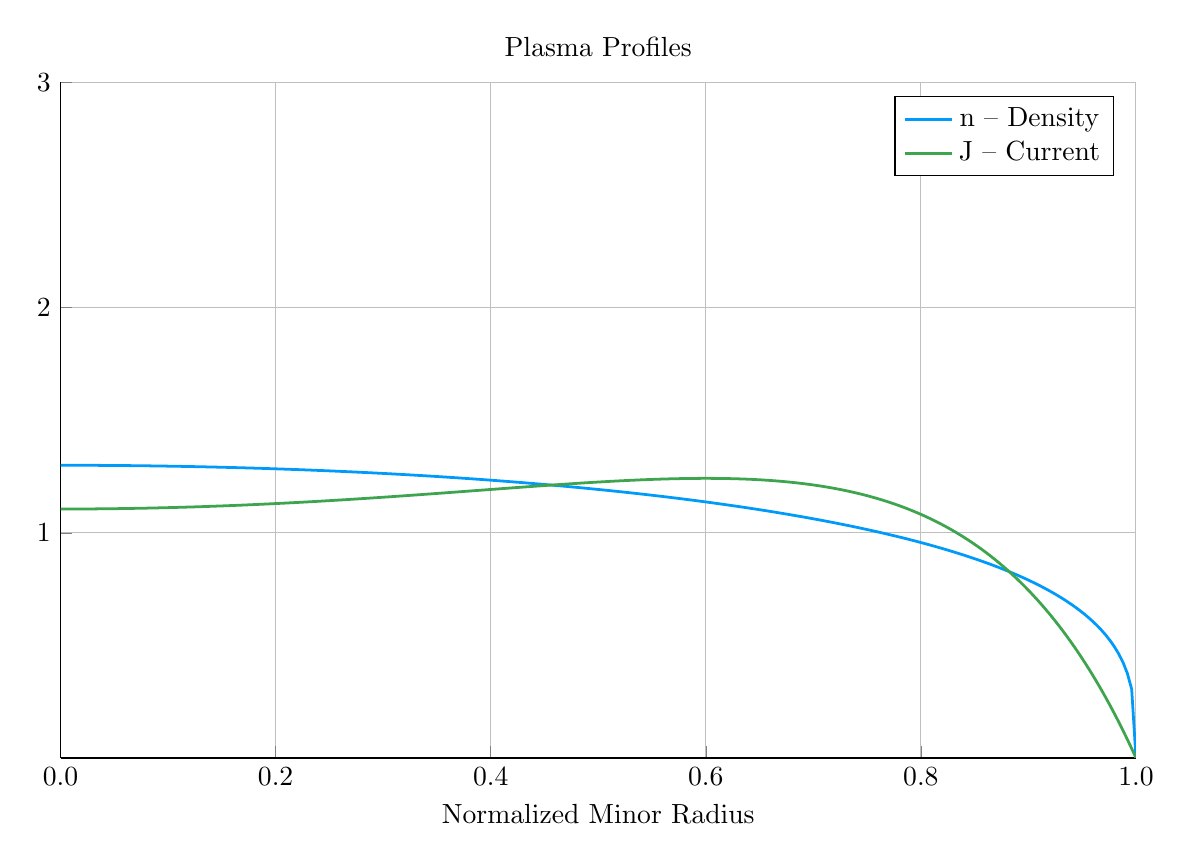
\begin{tikzpicture}[]
\begin{axis}[height = {101.6mm}, ylabel = {}, title = {Plasma Profiles}, xmin = {0.0}, xmax = {1.0}, ymax = {3}, xlabel = {Normalized Minor Radius}, {unbounded coords=jump, scaled x ticks = false, xticklabel style={rotate = 0}, xmajorgrids = true, xtick = {0.0,0.2,0.4,0.6000000000000001,0.8,1.0}, xticklabels = {0.0,0.2,0.4,0.6,0.8,1.0}, xtick align = inside, axis lines* = left, scaled y ticks = false, yticklabel style={rotate = 0}, ymajorgrids = true, ytick = {1.0,2.0,3.0}, yticklabels = {1,2,3}, ytick align = inside, axis lines* = left,     xshift = 0.0mm,
    yshift = 0.0mm,
    axis background/.style={fill={rgb,1:red,1.00000000;green,1.00000000;blue,1.00000000}}
}, ymin = {0}, width = {152.4mm}]\addplot+ [color = {rgb,1:red,0.00000000;green,0.60560316;blue,0.97868012},
draw opacity=1.0,
line width=1,
solid,mark = none,
mark size = 2.0,
mark options = {
    color = {rgb,1:red,0.00000000;green,0.00000000;blue,0.00000000}, draw opacity = 1.0,
    fill = {rgb,1:red,0.00000000;green,0.60560316;blue,0.97868012}, fill opacity = 1.0,
    line width = 1,
    rotate = 0,
    solid
}]coordinates {
(0.0, 1.3)
(0.004, 1.2999937599650557)
(0.008, 1.2999750394408758)
(0.012, 1.299943837169305)
(0.016, 1.2999001510530381)
(0.02, 1.2998439781550484)
(0.024, 1.2997753146977886)
(0.028, 1.2996941560621622)
(0.032, 1.2996004967862647)
(0.036, 1.2994943305638946)
(0.04, 1.2993756502428317)
(0.044, 1.2992444478228855)
(0.048, 1.2991007144537061)
(0.052, 1.2989444404323625)
(0.056, 1.2987756152006849)
(0.06, 1.2985942273423656)
(0.064, 1.2984002645798236)
(0.068, 1.2981937137708253)
(0.072, 1.2979745609048603)
(0.076, 1.2977427910992743)
(0.08, 1.2974983885951488)
(0.084, 1.2972413367529347)
(0.088, 1.2969716180478277)
(0.092, 1.2966892140648891)
(0.096, 1.2963941054939072)
(0.1, 1.2960862721239934)
(0.104, 1.2957656928379149)
(0.108, 1.2954323456061552)
(0.112, 1.295086207480701)
(0.116, 1.2947272545885533)
(0.12, 1.2943554621249538)
(0.124, 1.2939708043463278)
(0.128, 1.2935732545629344)
(0.132, 1.2931627851312222)
(0.136, 1.2927393674458851)
(0.14, 1.2923029719316104)
(0.144, 1.2918535680345185)
(0.148, 1.2913911242132843)
(0.152, 1.290915607929936)
(0.156, 1.2904269856403272)
(0.16, 1.2899252227842701)
(0.164, 1.289410283775332)
(0.168, 1.2888821319902795)
(0.172, 1.2883407297581677)
(0.176, 1.2877860383490682)
(0.18, 1.2872180179624235)
(0.184, 1.286636627715024)
(0.188, 1.286041825628597)
(0.192, 1.2854335686170009)
(0.196, 1.2848118124730112)
(0.2, 1.2841765118546966)
(0.204, 1.2835276202713661)
(0.208, 1.2828650900690854)
(0.212, 1.2821888724157464)
(0.216, 1.2814989172856817)
(0.22, 1.2807951734438123)
(0.224, 1.280077588429316)
(0.228, 1.2793461085388045)
(0.232, 1.2786006788089976)
(0.236, 1.2778412429988808)
(0.24, 1.2770677435713307)
(0.244, 1.2762801216741988)
(0.248, 1.275478317120833)
(0.252, 1.274662268370027)
(0.256, 1.2738319125053779)
(0.26, 1.2729871852140369)
(0.264, 1.2721280207648382)
(0.268, 1.2712543519857844)
(0.272, 1.2703661102408716)
(0.276, 1.2694632254062383)
(0.28, 1.268545625845612)
(0.284, 1.2676132383850391)
(0.288, 1.266665988286872)
(0.292, 1.2657037992229945)
(0.296, 1.2647265932472596)
(0.3, 1.2637342907671185)
(0.304, 1.262726810514414)
(0.308, 1.261704069515311)
(0.312, 1.2606659830593416)
(0.316, 1.2596124646675324)
(0.32, 1.2585434260595858)
(0.324, 1.257458777120088)
(0.328, 1.256358425863706)
(0.332, 1.2552422783993482)
(0.336, 1.2541102388932475)
(0.34, 1.2529622095309358)
(0.344, 1.2517980904780717)
(0.348, 1.2506177798400802)
(0.352, 1.24942117362057)
(0.356, 1.248208165678479)
(0.36, 1.2469786476839106)
(0.364, 1.2457325090726121)
(0.368, 1.2444696369990487)
(0.372, 1.2431899162880222)
(0.376, 1.2418932293847857)
(0.38, 1.2405794563035972)
(0.384, 1.239248474574658)
(0.388, 1.237900159189375)
(0.392, 1.2365343825438908)
(0.396, 1.2351510143808089)
(0.4, 1.2337499217290562)
(0.404, 1.2323309688418065)
(0.408, 1.2308940171323957)
(0.412, 1.229438925108151)
(0.416, 1.2279655483020526)
(0.42, 1.2264737392021483)
(0.424, 1.2249633471786308)
(0.428, 1.2234342184084848)
(0.432, 1.221886195797614)
(0.436, 1.2203191189003393)
(0.44, 1.2187328238361723)
(0.444, 1.2171271432037454)
(0.448, 1.2155019059917886)
(0.452, 1.2138569374870312)
(0.456, 1.212192059178898)
(0.46, 1.210507088660872)
(0.464, 1.208801839528379)
(0.468, 1.2070761212730492)
(0.472, 1.205329739173201)
(0.476, 1.2035624941803869)
(0.48, 1.2017741828018271)
(0.484, 1.1999645969785544)
(0.488, 1.1981335239590802)
(0.492, 1.1962807461683858)
(0.496, 1.1944060410720247)
(0.5, 1.1925091810351223)
(0.504, 1.190589933176035)
(0.508, 1.1886480592144295)
(0.512, 1.1866833153135188)
(0.516, 1.1846954519161883)
(0.52, 1.1826842135747218)
(0.524, 1.1806493387738237)
(0.528, 1.1785905597466213)
(0.532, 1.1765076022833005)
(0.536, 1.1744001855320279)
(0.54, 1.1722680217917714)
(0.544, 1.1701108162966227)
(0.548, 1.1679282669911981)
(0.552, 1.1657200642966656)
(0.556, 1.1634858908669246)
(0.56, 1.1612254213344295)
(0.564, 1.1589383220451273)
(0.568, 1.1566242507819302)
(0.572, 1.154282856476133)
(0.576, 1.1519137789061165)
(0.58, 1.1495166483826693)
(0.584, 1.1470910854201908)
(0.588, 1.1446367003930078)
(0.592, 1.142153093175977)
(0.596, 1.1396398527684999)
(0.6, 1.1370965569010092)
(0.604, 1.1345227716229302)
(0.608, 1.1319180508710498)
(0.612, 1.1292819360171518)
(0.616, 1.1266139553937018)
(0.62, 1.123913623796276)
(0.624, 1.1211804419613376)
(0.628, 1.1184138960178658)
(0.632, 1.1156134569112315)
(0.636, 1.1127785797976015)
(0.64, 1.1099087034070205)
(0.644, 1.1070032493731854)
(0.648, 1.1040616215277776)
(0.652, 1.1010832051570543)
(0.656, 1.0980673662182174)
(0.66, 1.0950134505129014)
(0.664, 1.0919207828148862)
(0.668, 1.0887886659489356)
(0.672, 1.0856163798173906)
(0.676, 1.082403180370883)
(0.68, 1.0791482985192302)
(0.684, 1.075850938978235)
(0.688, 1.0725102790477619)
(0.692, 1.0691254673160542)
(0.696, 1.0656956222848162)
(0.7, 1.0622198309091082)
(0.704, 1.0586971470455604)
(0.708, 1.055126589801824)
(0.712, 1.0515071417795323)
(0.716, 1.04783774720231)
(0.72, 1.0441173099195802)
(0.724, 1.0403446912760228)
(0.728, 1.03651870783555)
(0.732, 1.0326381289475657)
(0.736, 1.0287016741420443)
(0.74, 1.0247080103385948)
(0.744, 1.0206557488531367)
(0.748, 1.0165434421840995)
(0.752, 1.0123695805581145)
(0.756, 1.0081325882130072)
(0.76, 1.003830819393436)
(0.764, 0.9994625540317649)
(0.768, 0.9950259930836299)
(0.772, 0.990519253484107)
(0.776, 0.9859403626863661)
(0.78, 0.9812872527401133)
(0.784, 0.9765577538618856)
(0.788, 0.9717495874432898)
(0.792, 0.9668603584364187)
(0.796, 0.9618875470478029)
(0.8, 0.9568284996631833)
(0.804, 0.9516804189149115)
(0.808, 0.946440352791649)
(0.812, 0.9411051826759365)
(0.816, 0.9356716101787849)
(0.82, 0.9301361426212457)
(0.824, 0.9244950769904182)
(0.828, 0.9187444821708816)
(0.832, 0.9128801792212949)
(0.836, 0.9068977194288869)
(0.84, 0.900792359830521)
(0.844, 0.8945590358364464)
(0.848, 0.8881923305297794)
(0.852, 0.8816864401388146)
(0.856, 0.8750351350873486)
(0.86, 0.8682317159164477)
(0.864, 0.86126896323448)
(0.868, 0.8541390806843802)
(0.872, 0.8468336297096526)
(0.876, 0.8393434546426821)
(0.88, 0.8316585963161566)
(0.884, 0.8237681919917861)
(0.888, 0.81566035888456)
(0.892, 0.8073220579010558)
(0.896, 0.7987389333598728)
(0.9, 0.7898951233563103)
(0.904, 0.7807730339816926)
(0.908, 0.7713530686829113)
(0.912, 0.7616133014678136)
(0.916, 0.7515290791633757)
(0.92, 0.7410725331284098)
(0.924, 0.7302119741312908)
(0.928, 0.7189111346441375)
(0.932, 0.7071282092103691)
(0.936, 0.6948146236457978)
(0.94, 0.6819134341198397)
(0.944, 0.6683572117823803)
(0.948, 0.654065197526229)
(0.952, 0.6389393969490827)
(0.956, 0.6228590949732707)
(0.96, 0.6056729403361176)
(0.964, 0.5871871562979527)
(0.968, 0.5671473067124922)
(0.972, 0.5452087722509604)
(0.976, 0.520886146278826)
(0.98, 0.4934599473688843)
(0.984, 0.46178715390262587)
(0.988, 0.4238602013900372)
(0.992, 0.3755408186191309)
(0.996, 0.3052175562338072)
(1.0, 0.0)
};
\addlegendentry{n -- Density}
\addplot+ [color = {rgb,1:red,0.24222430;green,0.64327509;blue,0.30444865},
draw opacity=1.0,
line width=1,
solid,mark = none,
mark size = 2.0,
mark options = {
    color = {rgb,1:red,0.00000000;green,0.00000000;blue,0.00000000}, draw opacity = 1.0,
    fill = {rgb,1:red,0.24222430;green,0.64327509;blue,0.30444865}, fill opacity = 1.0,
    line width = 1,
    rotate = 0,
    solid
}]coordinates {
(0.0, 1.1055925931810484)
(0.004, 1.1056025434176453)
(0.008, 1.105632392966404)
(0.012, 1.1056821383432776)
(0.016, 1.1057517737383413)
(0.02, 1.1058412910110205)
(0.024, 1.1059506796834087)
(0.028, 1.106079926931665)
(0.032, 1.106229017575493)
(0.036, 1.1063979340656915)
(0.04, 1.106586656469768)
(0.044, 1.1067951624556105)
(0.048, 1.107023427273207)
(0.052, 1.1072714237343937)
(0.056, 1.1075391221906397)
(0.06, 1.107826490508826)
(0.064, 1.1081334940450354)
(0.068, 1.1084600956163122)
(0.072, 1.1088062554703932)
(0.076, 1.1091719312533783)
(0.08, 1.1095570779753314)
(0.084, 1.1099616479737875)
(0.088, 1.110385590875139)
(0.092, 1.1108288535538926)
(0.096, 1.1112913800897515)
(0.1, 1.1117731117225211)
(0.104, 1.1122739868047913)
(0.108, 1.112793940752376)
(0.112, 1.1133329059924844)
(0.116, 1.1138908119095834)
(0.12, 1.1144675847889256)
(0.124, 1.115063147757707)
(0.128, 1.1156774207238216)
(0.132, 1.1163103203121705)
(0.136, 1.1169617597984949)
(0.14, 1.1176316490406888)
(0.144, 1.11831989440755)
(0.148, 1.119026398704931)
(0.152, 1.11975106109924)
(0.156, 1.120493777038251)
(0.16, 1.1212544381691738)
(0.164, 1.1220329322539315)
(0.168, 1.1228291430816038)
(0.172, 1.1236429503779706)
(0.176, 1.1244742297121144)
(0.18, 1.1253228524000167)
(0.184, 1.1261886854050946)
(0.188, 1.127071591235615)
(0.192, 1.1279714278389303)
(0.196, 1.128888048492462)
(0.2, 1.1298213016913794)
(0.204, 1.1307710310328927)
(0.208, 1.131737075097102)
(0.212, 1.1327192673243216)
(0.216, 1.1337174358888118)
(0.22, 1.1347314035688367)
(0.224, 1.135760987612975)
(0.228, 1.136805999602598)
(0.232, 1.1378662453104351)
(0.236, 1.1389415245551366)
(0.24, 1.140031631051753)
(0.244, 1.1411363522580324)
(0.248, 1.1422554692164475)
(0.252, 1.143388756391854)
(0.256, 1.1445359815046836)
(0.26, 1.145696905359567)
(0.264, 1.146871281669287)
(0.268, 1.1480588568739498)
(0.272, 1.1492593699552682)
(0.276, 1.1504725522458386)
(0.28, 1.1516981272333027)
(0.284, 1.1529358103592642)
(0.288, 1.1541853088128475)
(0.292, 1.1554463213187653)
(0.296, 1.1567185379197655)
(0.3, 1.15800163975333)
(0.304, 1.1592952988224805)
(0.308, 1.160599177760553)
(0.312, 1.1619129295898027)
(0.316, 1.1632361974736778)
(0.32, 1.1645686144626213)
(0.324, 1.1659098032332398)
(0.328, 1.1672593758206753)
(0.332, 1.1686169333440195)
(0.336, 1.1699820657245965)
(0.34, 1.171354351396943)
(0.344, 1.1727333570123062)
(0.348, 1.1741186371344703)
(0.352, 1.1755097339277303)
(0.356, 1.176906176836817)
(0.36, 1.1783074822585666)
(0.364, 1.1797131532051435)
(0.368, 1.181122678958593)
(0.372, 1.1825355347165192)
(0.376, 1.1839511812286583)
(0.38, 1.1853690644241248)
(0.384, 1.1867886150290958)
(0.388, 1.1882092481746926)
(0.392, 1.1896303629948166)
(0.396, 1.1910513422136817)
(0.4, 1.1924715517227884)
(0.404, 1.1938903401470713)
(0.408, 1.1953070383999467)
(0.412, 1.1967209592269779)
(0.416, 1.198131396737873)
(0.42, 1.199537625926516)
(0.424, 1.2009389021787291)
(0.428, 1.2023344607674524)
(0.432, 1.2037235163350242)
(0.436, 1.205105262362225)
(0.44, 1.2064788706237588)
(0.444, 1.2078434906298132)
(0.448, 1.2091982490533475)
(0.452, 1.2105422491427469)
(0.456, 1.2118745701194584)
(0.46, 1.2131942665602276)
(0.464, 1.2145003677635429)
(0.468, 1.2157918770998737)
(0.472, 1.2170677713452926)
(0.476, 1.218326999998044)
(0.48, 1.219568484577629)
(0.484, 1.220791117905943)
(0.488, 1.2219937633700142)
(0.492, 1.2231752541658545)
(0.496, 1.2243343925229389)
(0.5, 1.2254699489088112)
(0.504, 1.2265806612132972)
(0.508, 1.227665233911794)
(0.512, 1.2287223372070952)
(0.516, 1.229750606149186)
(0.52, 1.2307486397324405)
(0.524, 1.2317149999696246)
(0.528, 1.2326482109421029)
(0.532, 1.2335467578256245)
(0.536, 1.234409085891052)
(0.54, 1.235233599479366)
(0.544, 1.2360186609502908)
(0.548, 1.2367625896038223)
(0.552, 1.2374636605739702)
(0.556, 1.2381201036939686)
(0.56, 1.2387301023322053)
(0.564, 1.2392917921981084)
(0.568, 1.2398032601171822)
(0.572, 1.2402625427743916)
(0.576, 1.2406676254250506)
(0.58, 1.241016440572357)
(0.584, 1.2413068666106932)
(0.588, 1.2415367264337844)
(0.592, 1.2417037860067774)
(0.596, 1.2418057529012922)
(0.6, 1.2418402747924557)
(0.604, 1.2418049379169072)
(0.608, 1.2416972654907381)
(0.612, 1.2415147160863034)
(0.616, 1.2412546819667964)
(0.62, 1.2409144873774753)
(0.624, 1.24049138679237)
(0.628, 1.2399825631152874)
(0.632, 1.239385125833895)
(0.636, 1.2386961091256128)
(0.64, 1.2379124699140391)
(0.644, 1.2370310858745734)
(0.648, 1.2360487533878732)
(0.652, 1.2349621854397481)
(0.656, 1.233768009466043)
(0.66, 1.2324627651410391)
(0.664, 1.2310429021078442)
(0.668, 1.2295047776492094)
(0.672, 1.2278446542971666)
(0.676, 1.2260586973798364)
(0.68, 1.224142972503699)
(0.684, 1.2220934429695933)
(0.688, 1.219905967120643)
(0.692, 1.2175762956202625)
(0.696, 1.2151000686583564)
(0.7, 1.2124728130837497)
(0.704, 1.2096899394608527)
(0.708, 1.206746739048499)
(0.712, 1.2036383806988336)
(0.716, 1.200359907674078)
(0.72, 1.1969062343789294)
(0.724, 1.1932721430062943)
(0.728, 1.1894522800939817)
(0.732, 1.1854411529899347)
(0.736, 1.181233126223481)
(0.74, 1.1768224177800433)
(0.744, 1.172203095276651)
(0.748, 1.1673690720355396)
(0.752, 1.162314103053033)
(0.756, 1.1570317808608346)
(0.76, 1.1515155312767646)
(0.764, 1.1457586090418983)
(0.768, 1.1397540933409778)
(0.772, 1.133494883202872)
(0.776, 1.1269736927777798)
(0.78, 1.1201830464877607)
(0.784, 1.1131152740470984)
(0.788, 1.1057625053488873)
(0.792, 1.0981166652141365)
(0.796, 1.0901694679995795)
(0.8, 1.0819124120602648)
(0.804, 1.0733367740628939)
(0.808, 1.064433603145756)
(0.812, 1.0551937149209845)
(0.816, 1.0456076853147525)
(0.82, 1.0356658442408755)
(0.824, 1.0253582691031793)
(0.828, 1.0146747781218477)
(0.832, 1.0036049234788245)
(0.836, 0.99213798427721)
(0.84, 0.980262959309437)
(0.844, 0.9679685596288679)
(0.848, 0.9552432009192925)
(0.852, 0.9420749956566505)
(0.856, 0.9284517450571373)
(0.86, 0.9143609308056804)
(0.864, 0.8997897065585966)
(0.868, 0.8847248892140719)
(0.872, 0.8691529499438978)
(0.876, 0.8530600049797328)
(0.88, 0.8364318061469402)
(0.884, 0.819253731138866)
(0.888, 0.8015107735241939)
(0.892, 0.783187532479819)
(0.896, 0.7642682022414483)
(0.9, 0.7447365612639053)
(0.904, 0.72457596108289)
(0.908, 0.7037693148696959)
(0.912, 0.6822990856701381)
(0.916, 0.6601472743186879)
(0.92, 0.6372954070185461)
(0.924, 0.6137245225781115)
(0.928, 0.5894151592940192)
(0.932, 0.564347341470635)
(0.936, 0.5385005655655922)
(0.94, 0.5118537859506463)
(0.944, 0.48438540027680593)
(0.948, 0.45607323443237957)
(0.952, 0.4268945270822218)
(0.956, 0.39682591377612964)
(0.96, 0.3658434106139833)
(0.964, 0.3339223974548356)
(0.968, 0.30103760065679763)
(0.972, 0.2671630753341644)
(0.976, 0.23227218711781)
(0.98, 0.19633759340448617)
(0.984, 0.15933122408020503)
(0.988, 0.12122426170246466)
(0.992, 0.08198712112559489)
(0.996, 0.04158942855305283)
(1.0, 0.0)
};
\addlegendentry{J -- Current}
\end{axis}

\end{tikzpicture}

		\end{adjustbox}
        \caption{Density and Current Profiles}
    \end{subfigure}
    \hfill
    \begin{subfigure}[t]{0.45\textwidth}
        \centering
		\begin{adjustbox}{width=\textwidth}
			\Large
			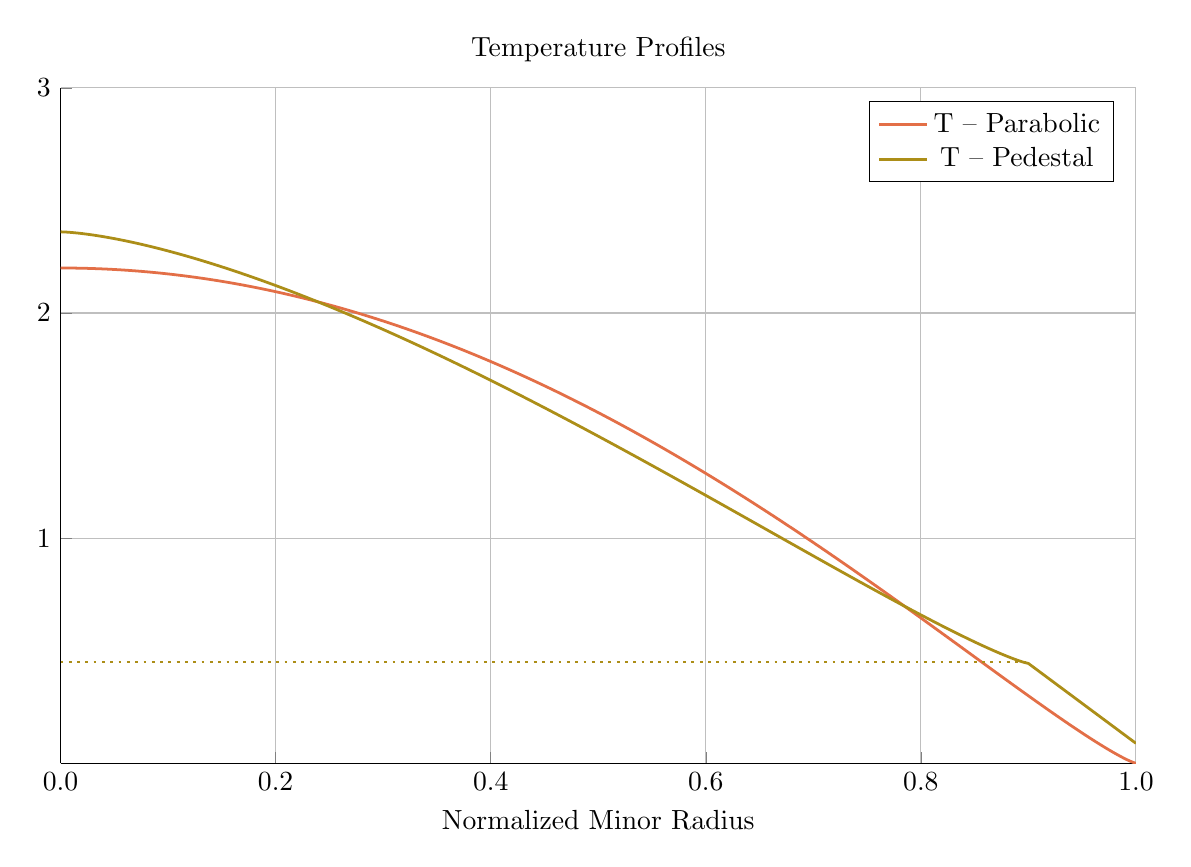
\begin{tikzpicture}[]
\begin{axis}[height = {101.6mm}, ylabel = {}, title = {Temperature Profiles}, xmin = {0.0}, xmax = {1.0}, ymax = {3}, xlabel = {Normalized Minor Radius}, {unbounded coords=jump, scaled x ticks = false, xticklabel style={rotate = 0}, xmajorgrids = true, xtick = {0.0,0.2,0.4,0.6000000000000001,0.8,1.0}, xticklabels = {0.0,0.2,0.4,0.6,0.8,1.0}, xtick align = inside, axis lines* = left, scaled y ticks = false, yticklabel style={rotate = 0}, ymajorgrids = true, ytick = {1.0,2.0,3.0}, yticklabels = {1,2,3}, ytick align = inside, axis lines* = left,     xshift = 0.0mm,
    yshift = 0.0mm,
    axis background/.style={fill={rgb,1:red,1.00000000;green,1.00000000;blue,1.00000000}}
}, ymin = {0}, width = {152.4mm}]\addplot+ [color = {rgb,1:red,0.88887350;green,0.43564919;blue,0.27812294},
draw opacity=1.0,
line width=1,
solid,mark = none,
mark size = 2.0,
mark options = {
    color = {rgb,1:red,0.00000000;green,0.00000000;blue,0.00000000}, draw opacity = 1.0,
    fill = {rgb,1:red,0.88887350;green,0.43564919;blue,0.27812294}, fill opacity = 1.0,
    line width = 1,
    rotate = 0,
    solid
}]coordinates {
(0.0, 2.2)
(0.004, 2.1999577600675844)
(0.008, 2.199831041081363)
(0.012, 2.199619845474514)
(0.016, 2.1993241773026853)
(0.02, 2.198944042244507)
(0.024, 2.1984794476023213)
(0.028, 2.1979304023031214)
(0.032, 2.1972969168996905)
(0.036, 2.196579003571959)
(0.04, 2.195776676128566)
(0.044, 2.194889950008634)
(0.048, 2.1939188422837517)
(0.052, 2.192863371660171)
(0.056, 2.1917235584812182)
(0.06, 2.1904994247299143)
(0.064, 2.189190994031813)
(0.068, 2.187798291658056)
(0.072, 2.1863213445286407)
(0.076, 2.1847601812159145)
(0.08, 2.1831148319482794)
(0.084, 2.1813853286141245)
(0.088, 2.179571704765981)
(0.092, 2.1776739956248985)
(0.096, 2.1756922380850554)
(0.1, 2.1736264707185855)
(0.104, 2.1714767337806498)
(0.108, 2.1692430692147298)
(0.112, 2.1669255206581606)
(0.116, 2.164524133447901)
(0.12, 2.1620389546265417)
(0.124, 2.1594700329485588)
(0.128, 2.1568174188868077)
(0.132, 2.154081164639269)
(0.136, 2.1512613241360428)
(0.14, 2.148357953046596)
(0.144, 2.1453711087872693)
(0.148, 2.1423008505290397)
(0.152, 2.139147239205551)
(0.156, 2.1359103375214086)
(0.16, 2.1325902099607443)
(0.164, 2.129186922796058)
(0.168, 2.1257005440973358)
(0.172, 2.1221311437414503)
(0.176, 2.1184787934218474)
(0.18, 2.1147435666585284)
(0.184, 2.1109255388083183)
(0.188, 2.1070247870754453)
(0.192, 2.1030413905224172)
(0.196, 2.098975430081212)
(0.2, 2.09482698856478)
(0.204, 2.090596150678874)
(0.208, 2.086283003034196)
(0.212, 2.0818876341588837)
(0.216, 2.0774101345113314)
(0.22, 2.072850596493357)
(0.224, 2.068209114463716)
(0.228, 2.063485784751976)
(0.232, 2.058680705672756)
(0.236, 2.053793977540332)
(0.24, 2.0488257026836245)
(0.244, 2.043775985461571)
(0.248, 2.038644932278893)
(0.252, 2.033432651602259)
(0.256, 2.0281392539768675)
(0.26, 2.022764852043437)
(0.264, 2.0173095605556335)
(0.268, 2.0117734963979244)
(0.272, 2.006156778603888)
(0.276, 2.0004595283749724)
(0.28, 1.9946818690997206)
(0.284, 1.9888239263734737)
(0.288, 1.9828858280185606)
(0.292, 1.976867704104986)
(0.296, 1.9707696869716258)
(0.3, 1.9645919112479475)
(0.304, 1.9583345138762616)
(0.308, 1.9519976341345224)
(0.312, 1.9455814136596863)
(0.316, 1.939085996471644)
(0.32, 1.932511528997742)
(0.324, 1.9258581600979061)
(0.328, 1.9191260410903783)
(0.332, 1.912315325778094)
(0.336, 1.9054261704757012)
(0.34, 1.8984587340372499)
(0.344, 1.8914131778845642)
(0.348, 1.8842896660363146)
(0.352, 1.8770883651378103)
(0.356, 1.8698094444915332)
(0.36, 1.8624530760884261)
(0.364, 1.8550194346399664)
(0.368, 1.8475086976110369)
(0.372, 1.839921045253621)
(0.376, 1.8322566606413475)
(0.38, 1.8245157297049002)
(0.384, 1.8166984412683274)
(0.388, 1.8088049870862715)
(0.392, 1.8008355618821434)
(0.396, 1.792790363387276)
(0.4, 1.7846695923810785)
(0.404, 1.776473452732227)
(0.408, 1.7682021514409176)
(0.412, 1.7598558986822177)
(0.416, 1.7514349078505493)
(0.42, 1.742939395605332)
(0.424, 1.7343695819178346)
(0.428, 1.725725690119258)
(0.432, 1.7170079469501018)
(0.436, 1.7082165826108464)
(0.44, 1.6993518308139948)
(0.444, 1.6904139288375197)
(0.448, 1.6814031175797635)
(0.452, 1.6723196416158315)
(0.456, 1.6631637492555364)
(0.46, 1.653935692602939)
(0.464, 1.6446357276175452)
(0.468, 1.6352641141772097)
(0.472, 1.6258211161428078)
(0.476, 1.6163070014247378)
(0.48, 1.606722042051314)
(0.484, 1.5970665142391203)
(0.488, 1.5873406984653924)
(0.492, 1.5775448795424998)
(0.496, 1.5676793466946068)
(0.5, 1.5577443936365882)
(0.504, 1.5477403186552856)
(0.508, 1.5376674246931867)
(0.512, 1.5275260194346267)
(0.516, 1.517316415394591)
(0.52, 1.5070389300102414)
(0.524, 1.4966938857352434)
(0.528, 1.4862816101370295)
(0.532, 1.4758024359970894)
(0.536, 1.465256701414425)
(0.54, 1.4546447499122863)
(0.544, 1.4439669305483216)
(0.548, 1.4332235980282817)
(0.552, 1.4224151128234246)
(0.556, 1.4115418412917677)
(0.56, 1.4006041558033582)
(0.564, 1.3896024348697198)
(0.568, 1.3785370632776597)
(0.572, 1.3674084322276236)
(0.576, 1.3562169394767907)
(0.58, 1.3449629894871216)
(0.584, 1.333646993578575)
(0.588, 1.3222693700877242)
(0.592, 1.3108305445320172)
(0.596, 1.2993309497799401)
(0.6, 1.2877710262273512)
(0.604, 1.2761512219802742)
(0.608, 1.2644719930444575)
(0.612, 1.2527338035220144)
(0.616, 1.2409371258154922)
(0.62, 1.2290824408397232)
(0.624, 1.2171702382418437)
(0.628, 1.2052010166298843)
(0.632, 1.1931752838103635)
(0.636, 1.1810935570353371)
(0.64, 1.1689563632593918)
(0.644, 1.156764239407098)
(0.648, 1.1445177326514693)
(0.652, 1.1322174007040144)
(0.656, 1.1198638121170017)
(0.66, 1.1074575465986056)
(0.664, 1.0949991953416336)
(0.668, 1.082489361366603)
(0.672, 1.0699286598799627)
(0.676, 1.0573177186483342)
(0.68, 1.044657178389695)
(0.684, 1.0319476931824922)
(0.688, 1.019189930893753)
(0.692, 1.0063845736273342)
(0.696, 0.9935323181935332)
(0.7, 0.980633876601379)
(0.704, 0.9676899765750238)
(0.708, 0.9547013620957563)
(0.712, 0.9416687939712927)
(0.716, 0.9285930504341149)
(0.72, 0.9154749277707805)
(0.724, 0.9023152409842818)
(0.728, 0.8891148244917015)
(0.732, 0.8758745328596077)
(0.736, 0.8625952415798288)
(0.74, 0.849277847888491)
(0.744, 0.8359232716314423)
(0.748, 0.822532456179475)
(0.752, 0.8091063693970627)
(0.756, 0.7956460046686752)
(0.76, 0.7821523819871128)
(0.764, 0.7686265491087244)
(0.768, 0.7550695827808527)
(0.772, 0.7414825900473649)
(0.776, 0.7278667096387308)
(0.78, 0.7142231134537544)
(0.784, 0.7005530081408239)
(0.788, 0.6868576367873601)
(0.792, 0.6731382807270975)
(0.796, 0.6593962614758839)
(0.8, 0.6456329428078906)
(0.804, 0.6318497329854856)
(0.808, 0.6180480871575735)
(0.812, 0.6042295099429783)
(0.816, 0.5903955582174578)
(0.82, 0.5765478441252689)
(0.824, 0.5626880383388612)
(0.828, 0.5488178735933505)
(0.832, 0.5349391485259877)
(0.836, 0.5210537318549578)
(0.84, 0.5071635669366619)
(0.844, 0.49327067674623953)
(0.848, 0.47937716933269775)
(0.852, 0.46548524380775297)
(0.856, 0.45159719693668826)
(0.86, 0.4377154304104124)
(0.864, 0.42384245889091393)
(0.868, 0.40998091893787963)
(0.872, 0.3961335789430169)
(0.876, 0.38230335022134865)
(0.88, 0.36849329943642983)
(0.884, 0.35470666257034567)
(0.888, 0.340946860691165)
(0.892, 0.3272175178224195)
(0.896, 0.31352248128407095)
(0.9, 0.2998658449561726)
(0.904, 0.28625197602028446)
(0.908, 0.2726855458667975)
(0.912, 0.25917156602852953)
(0.916, 0.24571543022609155)
(0.92, 0.23232296390814428)
(0.924, 0.21900048306792003)
(0.928, 0.20575486465742054)
(0.932, 0.1925936316637043)
(0.936, 0.17952505695042487)
(0.94, 0.16655829144594192)
(0.944, 0.15370352440467291)
(0.948, 0.14097218665156444)
(0.952, 0.12837721256189286)
(0.956, 0.11593338410667639)
(0.96, 0.10365779254585625)
(0.964, 0.09157047392306764)
(0.968, 0.07969531062880889)
(0.972, 0.06806135815914495)
(0.976, 0.056704888286093984)
(0.98, 0.04567272289384328)
(0.984, 0.035028106493367024)
(0.988, 0.024862215823612335)
(0.992, 0.0153206738078139)
(0.996, 0.0066847830139362754)
(1.0, 0.0)
};
\addlegendentry{T -- Parabolic}
\addplot+ [color = {rgb,1:red,0.67554396;green,0.55566233;blue,0.09423434},
draw opacity=1.0,
line width=1,
solid,mark = none,
mark size = 2.0,
mark options = {
    color = {rgb,1:red,0.00000000;green,0.00000000;blue,0.00000000}, draw opacity = 1.0,
    fill = {rgb,1:red,0.67554396;green,0.55566233;blue,0.09423434}, fill opacity = 1.0,
    line width = 1,
    rotate = 0,
    solid
}]coordinates {
(0.0, 2.3605919704710323)
(0.004, 2.359910398918797)
(0.008, 2.3586642994783618)
(0.012, 2.3570508613498493)
(0.016, 2.3551405297956594)
(0.02, 2.3529740696983454)
(0.024, 2.350579025743975)
(0.028, 2.3479756517769723)
(0.032, 2.3451796682823796)
(0.036, 2.342203747147281)
(0.04, 2.3390583928390996)
(0.044, 2.3357525032801973)
(0.048, 2.332293746279636)
(0.052, 2.328688822918463)
(0.056, 2.3249436581415552)
(0.06, 2.3210635425572748)
(0.064, 2.3170532404255844)
(0.068, 2.3129170735482543)
(0.072, 2.3086589875663335)
(0.076, 2.3042826051438894)
(0.08, 2.299791269197131)
(0.084, 2.295188078444673)
(0.088, 2.2904759169492626)
(0.092, 2.2856574788975115)
(0.096, 2.2807352895619175)
(0.1, 2.2757117231701707)
(0.104, 2.2705890182452353)
(0.108, 2.2653692908590712)
(0.112, 2.260054546151598)
(0.116, 2.2546466883966962)
(0.12, 2.2491475298430212)
(0.124, 2.243558798515241)
(0.128, 2.237882145128044)
(0.132, 2.2321191492388524)
(0.136, 2.2262713247439767)
(0.14, 2.220340124805883)
(0.144, 2.2143269462853388)
(0.148, 2.2082331337408316)
(0.152, 2.202059983048349)
(0.156, 2.1958087446868073)
(0.16, 2.189480626728042)
(0.164, 2.1830767975648464)
(0.168, 2.176598388406032)
(0.172, 2.1700464955636813)
(0.176, 2.163422182554496)
(0.18, 2.1567264820344176)
(0.184, 2.149960397583317)
(0.188, 2.14312490535454)
(0.192, 2.1362209556023704)
(0.196, 2.1292494740989305)
(0.2, 2.1222113634507807)
(0.204, 2.1151075043243255)
(0.208, 2.1079387565881396)
(0.212, 2.1007059603794906)
(0.216, 2.0934099371015487)
(0.22, 2.0860514903571366)
(0.224, 2.0786314068242686)
(0.228, 2.0711504570782133)
(0.232, 2.063609396364366)
(0.236, 2.0560089653257996)
(0.24, 2.0483498906890096)
(0.244, 2.040632885911039)
(0.248, 2.0328586517908898)
(0.252, 2.0250278770478602)
(0.256, 2.0171412388692334)
(0.26, 2.009199403429513)
(0.264, 2.00120302638324)
(0.268, 1.9931527533332325)
(0.272, 1.9850492202759686)
(0.276, 1.97689305402566)
(0.28, 1.9686848726184767)
(0.284, 1.9604252856982425)
(0.288, 1.9521148948848384)
(0.292, 1.9437542941264454)
(0.296, 1.9353440700366855)
(0.3, 1.9268848022176337)
(0.304, 1.9183770635696087)
(0.308, 1.9098214205885893)
(0.312, 1.9012184336520364)
(0.316, 1.8925686572938556)
(0.32, 1.883872640469185)
(0.324, 1.8751309268096423)
(0.328, 1.8663440548696335)
(0.332, 1.8575125583642822)
(0.336, 1.8486369663995004)
(0.34, 1.839717803694704)
(0.344, 1.8307555907986295)
(0.348, 1.8217508442986934)
(0.352, 1.812704077024307)
(0.356, 1.8036157982445404)
(0.36, 1.7944865138605)
(0.364, 1.7853167265927747)
(0.368, 1.776106936164285)
(0.372, 1.7668576394788444)
(0.376, 1.7575693307957496)
(0.38, 1.74824250190067)
(0.384, 1.7388776422731294)
(0.388, 1.7294752392508332)
(0.392, 1.7200357781911024)
(0.396, 1.7105597426296557)
(0.4, 1.7010476144369753)
(0.404, 1.6914998739724885)
(0.408, 1.6819170002367874)
(0.412, 1.6722994710220926)
(0.416, 1.6626477630611856)
(0.42, 1.6529623521750014)
(0.424, 1.6432437134190898)
(0.428, 1.633492321229143)
(0.432, 1.6237086495657764)
(0.436, 1.6138931720587668)
(0.44, 1.6040463621509233)
(0.444, 1.5941686932417938)
(0.448, 1.584260638831387)
(0.452, 1.5743226726641009)
(0.456, 1.5643552688730447)
(0.46, 1.5543589021249482)
(0.464, 1.544334047765842)
(0.468, 1.5342811819677138)
(0.472, 1.5242007818763206)
(0.476, 1.5140933257603746)
(0.48, 1.5039592931622903)
(0.484, 1.4937991650507099)
(0.488, 1.4836134239750187)
(0.492, 1.473402554222062)
(0.496, 1.4631670419753044)
(0.5, 1.4529073754766455)
(0.504, 1.4426240451911474)
(0.508, 1.4323175439749165)
(0.512, 1.4219883672464035)
(0.516, 1.4116370131613858)
(0.52, 1.4012639827919213)
(0.524, 1.3908697803095635)
(0.528, 1.3804549131731465)
(0.532, 1.3700198923214701)
(0.536, 1.359565232371216)
(0.54, 1.349091451820459)
(0.544, 1.3385990732581485)
(0.548, 1.328088623579961)
(0.552, 1.3175606342109392)
(0.556, 1.307015641335371)
(0.56, 1.2964541861343752)
(0.564, 1.2858768150316933)
(0.568, 1.2752840799482301)
(0.572, 1.2646765385659007)
(0.576, 1.2540547546013914)
(0.58, 1.2434192980904786)
(0.584, 1.2327707456835955)
(0.588, 1.222109680953382)
(0.592, 1.211436694715004)
(0.596, 1.200752385360086)
(0.6, 1.1900573592051713)
(0.604, 1.1793522308556705)
(0.608, 1.1686376235863563)
(0.612, 1.1579141697395272)
(0.616, 1.1471825111420575)
(0.62, 1.1364432995426441)
(0.624, 1.1256971970706737)
(0.628, 1.1149448767182386)
(0.632, 1.1041870228469695)
(0.636, 1.093424331721486)
(0.64, 1.0826575120714315)
(0.644, 1.0718872856842108)
(0.648, 1.061114388030769)
(0.652, 1.0503395689269308)
(0.656, 1.039563593233075)
(0.66, 1.0287872415951647)
(0.664, 1.0180113112304485)
(0.668, 1.0072366167614726)
(0.672, 0.9964639911023957)
(0.676, 0.9856942864020085)
(0.68, 0.9749283750483018)
(0.684, 0.9641671507399459)
(0.688, 0.9534115296306018)
(0.692, 0.9426624515526333)
(0.696, 0.9319208813275146)
(0.7, 0.9211878101710503)
(0.704, 0.9104642572024598)
(0.708, 0.8997512710674346)
(0.712, 0.8890499316865009)
(0.716, 0.8783613521413978)
(0.72, 0.8676866807137728)
(0.724, 0.8570271030923351)
(0.728, 0.8463838447667099)
(0.732, 0.8357581736286817)
(0.736, 0.8251514028043623)
(0.74, 0.8145648937441141)
(0.744, 0.8040000596009286)
(0.748, 0.7934583689324995)
(0.752, 0.7829413497675711)
(0.756, 0.7724505940834616)
(0.76, 0.7619877627491815)
(0.764, 0.7515545909975108)
(0.768, 0.741152894500166)
(0.772, 0.7307845761331225)
(0.776, 0.7204516335348546)
(0.78, 0.710156167579369)
(0.784, 0.6999003919093338)
(0.788, 0.6896866437035094)
(0.792, 0.6795173958885602)
(0.796, 0.6693952710502226)
(0.8, 0.6593230573553601)
(0.804, 0.6493037268683398)
(0.808, 0.6393404567373293)
(0.812, 0.6294366538454373)
(0.816, 0.6195959836776518)
(0.82, 0.6098224043609094)
(0.824, 0.6001202071108945)
(0.828, 0.5904940646939226)
(0.832, 0.58094909002811)
(0.836, 0.5714909077694643)
(0.84, 0.562125742755608)
(0.844, 0.5528605306710853)
(0.848, 0.5437030585117963)
(0.852, 0.5346621457948362)
(0.856, 0.5257478827341294)
(0.86, 0.516971950132737)
(0.864, 0.5083480600719166)
(0.868, 0.49989258164201933)
(0.872, 0.4916254625709785)
(0.876, 0.48357164972903754)
(0.88, 0.47576340897240366)
(0.884, 0.4682444150948954)
(0.888, 0.4610777748740693)
(0.892, 0.45436452608473005)
(0.896, 0.44830036952087016)
(0.9, 0.44361517600666117)
(0.904, 0.429419490374448)
(0.908, 0.41522380474223486)
(0.912, 0.4010281191100217)
(0.916, 0.38683243347780855)
(0.92, 0.3726367478455953)
(0.924, 0.3584410622133822)
(0.928, 0.34424537658116894)
(0.932, 0.3300496909489558)
(0.936, 0.3158540053167426)
(0.94, 0.30165831968452983)
(0.944, 0.28746263405231665)
(0.948, 0.27326694842010346)
(0.952, 0.2590712627878903)
(0.956, 0.24487557715567715)
(0.96, 0.23067989152346396)
(0.964, 0.21648420589125078)
(0.968, 0.2022885202590376)
(0.972, 0.18809283462682444)
(0.976, 0.17389714899461126)
(0.98, 0.1597014633623981)
(0.984, 0.14550577773018494)
(0.988, 0.13131009209797176)
(0.992, 0.11711440646575859)
(0.996, 0.1029187208335454)
(1.0, 0.08872303520133223)
};
\addlegendentry{T -- Pedestal}
\addplot+ [color = {rgb,1:red,0.67554396;green,0.55566233;blue,0.09423434},
draw opacity=1.0,
line width=1,
dotted,mark = none,
mark size = 2.0,
mark options = {
    color = {rgb,1:red,0.00000000;green,0.00000000;blue,0.00000000}, draw opacity = 1.0,
    fill = {rgb,1:red,0.67554396;green,0.55566233;blue,0.09423434}, fill opacity = 1.0,
    line width = 1,
    rotate = 0,
    solid
},forget plot]coordinates {
(0.0, 0.45)
(0.9, 0.45)
};
\end{axis}

\end{tikzpicture}

		\end{adjustbox}
        \caption{Temperature Profiles}
    \end{subfigure}
    \hfill \hfill ~\\ ~\\ ~\\
    \caption{Radial Plasma Profiles} ~\\
    \small The three most fundamental \replaced{profiles}{properties} of a fusion plasma are its temperature, density, and current. These \deleted{profiles} allow the model to reduce from three dimensions to \added{just} half of one.
\end{figure*}

\subsubsection{The Density Profile}

To begin, density has the simplest profile. This is because it is relatively flat, remaining near the average value -- $\overline n$ -- throughout the body of the plasma until quickly decaying to zero near the edge of the plasma.\footnote{Even in H-Mode plasmas where density profiles have a pedestal,\cite{density} they usually have much less of a peak than temperatures\cite{temperature} -- especially so in a reactor setting.\cite{pedestals}} For this reason, a parabolic profile with a very low peaking factor -- $\nu_n$ -- is well suited.
\begin{equation}
	n(\rho) = \overline n \cdot ( 1 + \nu_n ) \, \cdot ( 1 - \rho ^ 2 ) ^ {\nu_n}
\end{equation}
\myequations{Density Profile -- $n$}
\added{The reason $\overline n$ is referred to as the volume-averaged density is because using the volume integral -- given by \cref{eq:qv} -- over the density profile results in that value after dividing through by the volume ($\volume$):} 
\begin{equation}
	\overline n = \frac{ \int n(\vec{\bold{r}}) \, d\vec{\bold{r}}  }{\volume}
\end{equation}
\added{A final point to make is this parabolic profile allows for a short closed-form relation for the Greenwald density limit -- substantially simplifying this fusion systems model.} 

\subsubsection{The Temperature Profile}

The use of a parabolic profile for the plasma temperature is slightly more dubious. This is because H-Mode plasmas are actually highly peaked at the center, decaying to a non-zero pedestal temperature near the edge before finally dropping sharply to zero. This model chooses to forego this pedestal representation for a simple parabolic one -- although the pedestal approach is discussed in \cref{chapter:profiles}. Analogous to the density, the profile treats $\overline T$ as the average value and $\nu_T$ as the peaking parameter.
\begin{equation}
	T(\rho) = \overline T \cdot ( 1 + \nu_T ) \, \cdot ( 1 - \rho ^ 2 ) ^ {\nu_T}
\end{equation}
\myequations{Temperature Profile -- $T$}

\subsubsection{The Current \added{Density} Profile}

The plasma current \added{density} is the third profile and cannot safely be represented by a simple parabola. This is because having an adequate bootstrap current relies heavily on a profile being peaked off-axis -- i.e.\ at some radius not at the center. This hollow profile can then be modeled with the commonly given plasma internal inductance ($l_i$). Concretely, the current's hollow profile is described by:
\begin{equation}
	J(\rho) = \bar{J} \cdot \frac{ \gamma ^ 2 \cdot ( 1 - \rho ^ 2 ) \cdot e^{ \gamma \rho^2 } }{ e^\gamma - 1 - \gamma}
\end{equation}
\myequations{Current Profile -- $J$}
The intermediate $\gamma$ quantity can then be numerically solved for from the plasma internal inductance using the following relations -- with $b_p$ representing the normalized poloidal magnetic field. \added{These are derived in \cref{chapter:bootstrap}.}
\begin{equation}
	l_i = \frac{4 \kappa}{1+\kappa^2}	 \int_0^1 b_p^2 \, \rho \, d\rho
\end{equation}
\myequations{Internal Inductance -- $l_i$}
\begin{equation}
	\label{eq:b_p}
	b_p(\rho) = \frac{ -e^{\gamma\rho^2} ( \gamma\rho^2 - 1 - \gamma ) - 1 - \gamma }{\rho \,( e^\gamma - 1 - \gamma ) }
\end{equation}
\myequations{Normalized Poloidal Magnetic Field -- $b_p$}
Combined, these three geometric parameters and profiles lay the foundation for this zero-dimensional fusion systems model.

\section{Solving the Steady Current}

As suggested, one of the most important equations in a fusion reactor is current balance. In steady-state operation, all of a plasma's current ($I_P$) must come from a combination of its own bootstrap current ($I_{BS}$), as well as auxiliary current drive ($I_{CD}$). This can be represented mathematically as:
\begin{equation}
	\label{eq:ibal}
	\tcboxmath{
	I_P = I_{BS} + I_{CD}
	}
\end{equation}
\myequations{Current Balance -- $I$}
The goal is then to write equations for bootstrap current and driven current. This will make heavy use of the Greenwald density limit. \replaced{The steady current will then be}{Without spoiling too much, the steady current is} shown to be only a function of temperature! In other words, this current is independent of a tokamak's geometry and magnet strength. As will be pointed out then, though, a subtlety arises that will bring the two back into the picture -- self-consistency in the current drive efficiency ($\eta_{CD}$).

\subsection{Enforcing the Greenwald Density Limit}

The Greenwald density limit is \replaced{a density limit that applies to all tokamaks}{ubiquitous in the field of fusion energy.} It sets a hard limit on the density and how it scales with current and reactor size. Although currently lacking a true first-principles theoretical explanation, it does have a real meaning within the design context. Operate at too low a density and run the risk of never entering H-Mode. Run the density too high, and cause the tokamak's plasma to \replaced{disrupt.}{disrupt catastrophically!} \added{These conclusions can be seen in \cref{fig:greenwald}.}

\begin{figure*}
    \centering
    \hfill 
    \begin{subfigure}[t]{0.45\textwidth}
        \centering
		\begin{adjustbox}{width=\textwidth}
			\Large
			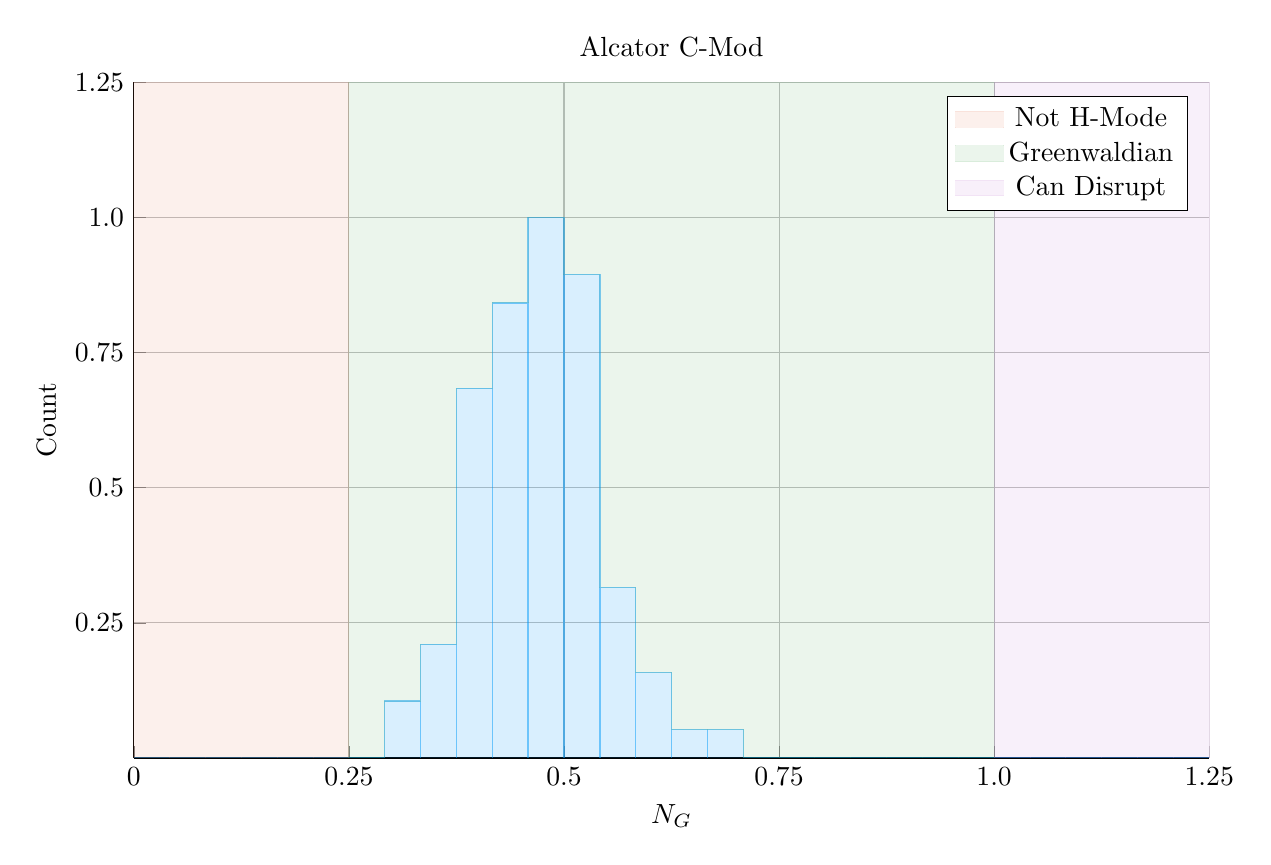
\begin{tikzpicture}[]
\begin{axis}[height = {101.6mm}, ylabel = {Count}, title = {Alcator C-Mod}, xmin = {0}, xmax = {1.25}, ymax = {1.25}, xlabel = {$N_G$}, {unbounded coords=jump, scaled x ticks = false, xticklabel style={rotate = 0}, xmajorgrids = true, xtick = {0.0,0.25,0.5,0.75,1.0,1.25}, xticklabels = {0,0.25,0.5,0.75,1.0,1.25}, xtick align = inside, axis lines* = left, scaled y ticks = false, yticklabel style={rotate = 0}, ymajorgrids = true, ytick = {0.0,0.25,0.5,0.75,1.0,1.25}, yticklabels = {,0.25,0.5,0.75,1.0,1.25}, ytick align = inside, axis lines* = left,     xshift = 0.0mm,
    yshift = 0.0mm,
    axis background/.style={fill={rgb,1:red,1.00000000;green,1.00000000;blue,1.00000000}}
}, ymin = {0}, width = {152.4mm}]\addplot+ [color = {rgb,1:red,0.00000000;green,0.60560316;blue,0.97868012},
draw opacity=0.5,
line width=0.5,
solid,mark = none,
mark size = 2.0,
mark options = {
    color = {rgb,1:red,0.00000000;green,0.00000000;blue,0.00000000}, draw opacity = 0.5,
    fill = {rgb,1:red,0.00000000;green,0.60560316;blue,0.97868012}, fill opacity = 0.5,
    line width = 1,
    rotate = 0,
    solid
},fill = {rgb,1:red,0.00000000;green,0.60560316;blue,0.97868012}, fill opacity=0.15,forget plot]coordinates {
(0.0, 0.0)
(0.0, 0.0)
(0.041666666666666664, 0.0)
(0.041666666666666664, 0.0)
(NaN, NaN)
(0.041666666666666664, 0.0)
(0.041666666666666664, 0.0)
(0.08333333333333333, 0.0)
(0.08333333333333333, 0.0)
(NaN, NaN)
(0.08333333333333333, 0.0)
(0.08333333333333333, 0.0)
(0.125, 0.0)
(0.125, 0.0)
(NaN, NaN)
(0.125, 0.0)
(0.125, 0.0)
(0.16666666666666666, 0.0)
(0.16666666666666666, 0.0)
(NaN, NaN)
(0.16666666666666666, 0.0)
(0.16666666666666666, 0.0)
(0.20833333333333334, 0.0)
(0.20833333333333334, 0.0)
(NaN, NaN)
(0.20833333333333334, 0.0)
(0.20833333333333334, 0.0)
(0.25, 0.0)
(0.25, 0.0)
(NaN, NaN)
(0.25, 0.0)
(0.25, 0.0)
(0.2916666666666667, 0.0)
(0.2916666666666667, 0.0)
(NaN, NaN)
(0.2916666666666667, 0.0)
(0.2916666666666667, 0.10526315789473684)
(0.3333333333333333, 0.10526315789473684)
(0.3333333333333333, 0.0)
(NaN, NaN)
(0.3333333333333333, 0.0)
(0.3333333333333333, 0.21052631578947367)
(0.375, 0.21052631578947367)
(0.375, 0.0)
(NaN, NaN)
(0.375, 0.0)
(0.375, 0.6842105263157895)
(0.4166666666666667, 0.6842105263157895)
(0.4166666666666667, 0.0)
(NaN, NaN)
(0.4166666666666667, 0.0)
(0.4166666666666667, 0.8421052631578947)
(0.4583333333333333, 0.8421052631578947)
(0.4583333333333333, 0.0)
(NaN, NaN)
(0.4583333333333333, 0.0)
(0.4583333333333333, 1.0)
(0.5, 1.0)
(0.5, 0.0)
(NaN, NaN)
(0.5, 0.0)
(0.5, 0.8947368421052632)
(0.5416666666666666, 0.8947368421052632)
(0.5416666666666666, 0.0)
(NaN, NaN)
(0.5416666666666666, 0.0)
(0.5416666666666666, 0.3157894736842105)
(0.5833333333333334, 0.3157894736842105)
(0.5833333333333334, 0.0)
(NaN, NaN)
(0.5833333333333334, 0.0)
(0.5833333333333334, 0.15789473684210525)
(0.625, 0.15789473684210525)
(0.625, 0.0)
(NaN, NaN)
(0.625, 0.0)
(0.625, 0.05263157894736842)
(0.6666666666666666, 0.05263157894736842)
(0.6666666666666666, 0.0)
(NaN, NaN)
(0.6666666666666666, 0.0)
(0.6666666666666666, 0.05263157894736842)
(0.7083333333333334, 0.05263157894736842)
(0.7083333333333334, 0.0)
(NaN, NaN)
(0.7083333333333334, 0.0)
(0.7083333333333334, 0.0)
(0.75, 0.0)
(0.75, 0.0)
(NaN, NaN)
(0.75, 0.0)
(0.75, 0.0)
(0.7916666666666666, 0.0)
(0.7916666666666666, 0.0)
(NaN, NaN)
(0.7916666666666666, 0.0)
(0.7916666666666666, 0.0)
(0.8333333333333334, 0.0)
(0.8333333333333334, 0.0)
(NaN, NaN)
(0.8333333333333334, 0.0)
(0.8333333333333334, 0.0)
(0.875, 0.0)
(0.875, 0.0)
(NaN, NaN)
(0.875, 0.0)
(0.875, 0.0)
(0.9166666666666666, 0.0)
(0.9166666666666666, 0.0)
(NaN, NaN)
(0.9166666666666666, 0.0)
(0.9166666666666666, 0.0)
(0.9583333333333334, 0.0)
(0.9583333333333334, 0.0)
(NaN, NaN)
(0.9583333333333334, 0.0)
(0.9583333333333334, 0.0)
(1.0, 0.0)
(1.0, 0.0)
(NaN, NaN)
(1.0, 0.0)
(1.0, 0.0)
(1.0416666666666667, 0.0)
(1.0416666666666667, 0.0)
(NaN, NaN)
(1.0416666666666667, 0.0)
(1.0416666666666667, 0.0)
(1.0833333333333333, 0.0)
(1.0833333333333333, 0.0)
(NaN, NaN)
(1.0833333333333333, 0.0)
(1.0833333333333333, 0.0)
(1.125, 0.0)
(1.125, 0.0)
(NaN, NaN)
(1.125, 0.0)
(1.125, 0.0)
(1.1666666666666667, 0.0)
(1.1666666666666667, 0.0)
(NaN, NaN)
(1.1666666666666667, 0.0)
(1.1666666666666667, 0.0)
(1.2083333333333333, 0.0)
(1.2083333333333333, 0.0)
(NaN, NaN)
(1.2083333333333333, 0.0)
(1.2083333333333333, 0.0)
(1.25, 0.0)
(1.25, 0.0)
(NaN, NaN)
};
\addplot+ [color = {rgb,1:red,0.88887350;green,0.43564919;blue,0.27812294},
draw opacity=0.1,
line width=0,
solid,mark = none,
mark size = 2.0,
mark options = {
    color = {rgb,1:red,0.00000000;green,0.00000000;blue,0.00000000}, draw opacity = 0.1,
    fill = {rgb,1:red,0.88887350;green,0.43564919;blue,0.27812294}, fill opacity = 0.1,
    line width = 1,
    rotate = 0,
    solid
},fill = {rgb,1:red,0.88887350;green,0.43564919;blue,0.27812294}, fill opacity=0.1,area legend]coordinates {
(0.0, 1.25)
(0.0, 0.0)
(0.041666666666666664, 0.0)
(0.041666666666666664, 0.0)
(0.08333333333333333, 0.0)
(0.08333333333333333, 0.0)
(0.125, 0.0)
(0.125, 0.0)
(0.16666666666666666, 0.0)
(0.16666666666666666, 0.0)
(0.20833333333333334, 0.0)
(0.20833333333333334, 0.0)
(0.25, 0.0)
(0.25, 1.25)
(0.0, 1.25)
};
\addlegendentry{Not H-Mode}
\addplot+ [color = {rgb,1:red,0.24222430;green,0.64327509;blue,0.30444865},
draw opacity=0.1,
line width=0,
solid,mark = none,
mark size = 2.0,
mark options = {
    color = {rgb,1:red,0.00000000;green,0.00000000;blue,0.00000000}, draw opacity = 0.1,
    fill = {rgb,1:red,0.24222430;green,0.64327509;blue,0.30444865}, fill opacity = 0.1,
    line width = 1,
    rotate = 0,
    solid
},fill = {rgb,1:red,0.24222430;green,0.64327509;blue,0.30444865}, fill opacity=0.1,area legend]coordinates {
(0.25, 1.25)
(0.25, 0.0)
(0.2916666666666667, 0.0)
(0.2916666666666667, 0.10526315789473684)
(0.3333333333333333, 0.10526315789473684)
(0.3333333333333333, 0.21052631578947367)
(0.375, 0.21052631578947367)
(0.375, 0.6842105263157895)
(0.4166666666666667, 0.6842105263157895)
(0.4166666666666667, 0.8421052631578947)
(0.4583333333333333, 0.8421052631578947)
(0.4583333333333333, 1.0)
(0.5, 1.0)
(0.5, 0.8947368421052632)
(0.5416666666666666, 0.8947368421052632)
(0.5416666666666666, 0.3157894736842105)
(0.5833333333333334, 0.3157894736842105)
(0.5833333333333334, 0.15789473684210525)
(0.625, 0.15789473684210525)
(0.625, 0.05263157894736842)
(0.6666666666666666, 0.05263157894736842)
(0.6666666666666666, 0.05263157894736842)
(0.7083333333333334, 0.05263157894736842)
(0.7083333333333334, 0.0)
(0.75, 0.0)
(0.75, 0.0)
(0.7916666666666666, 0.0)
(0.7916666666666666, 0.0)
(0.8333333333333334, 0.0)
(0.8333333333333334, 0.0)
(0.875, 0.0)
(0.875, 0.0)
(0.9166666666666666, 0.0)
(0.9166666666666666, 0.0)
(0.9583333333333334, 0.0)
(0.9583333333333334, 0.0)
(1.0, 0.0)
(1.0, 1.25)
(0.25, 1.25)
};
\addlegendentry{Greenwaldian}
\addplot+ [color = {rgb,1:red,0.76444018;green,0.44411178;blue,0.82429754},
draw opacity=0.1,
line width=0,
solid,mark = none,
mark size = 2.0,
mark options = {
    color = {rgb,1:red,0.00000000;green,0.00000000;blue,0.00000000}, draw opacity = 0.1,
    fill = {rgb,1:red,0.76444018;green,0.44411178;blue,0.82429754}, fill opacity = 0.1,
    line width = 1,
    rotate = 0,
    solid
},fill = {rgb,1:red,0.76444018;green,0.44411178;blue,0.82429754}, fill opacity=0.1,area legend]coordinates {
(1.0, 1.25)
(1.0, 0.0)
(1.0416666666666667, 0.0)
(1.0416666666666667, 0.0)
(1.0833333333333333, 0.0)
(1.0833333333333333, 0.0)
(1.125, 0.0)
(1.125, 0.0)
(1.1666666666666667, 0.0)
(1.1666666666666667, 0.0)
(1.2083333333333333, 0.0)
(1.2083333333333333, 0.0)
(1.25, 0.0)
(1.25, 1.25)
(1.0, 1.25)
};
\addlegendentry{Can Disrupt}
\end{axis}

\end{tikzpicture}

		\end{adjustbox}
        \caption{C-Mod}
    \end{subfigure}
    \hfill
    \begin{subfigure}[t]{0.45\textwidth}
        \centering
		\begin{adjustbox}{width=\textwidth}
			\Large
			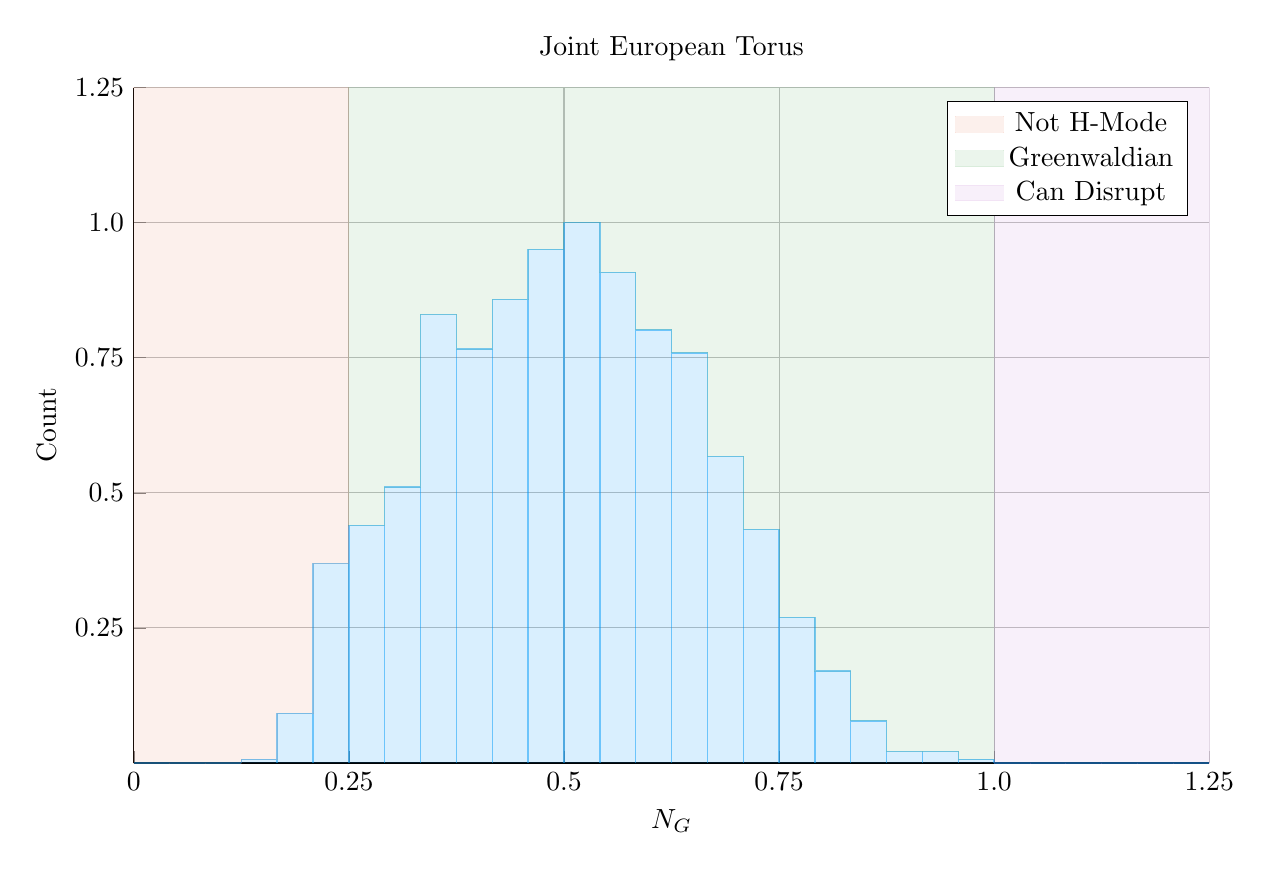
\begin{tikzpicture}[]
\begin{axis}[height = {101.6mm}, ylabel = {Count}, title = {Joint European Torus}, xmin = {0}, xmax = {1.25}, ymax = {1.25}, xlabel = {$N_G$}, {unbounded coords=jump, scaled x ticks = false, xticklabel style={rotate = 0}, xmajorgrids = true, xtick = {0.0,0.25,0.5,0.75,1.0,1.25}, xticklabels = {0,0.25,0.5,0.75,1.0,1.25}, xtick align = inside, axis lines* = left, scaled y ticks = false, yticklabel style={rotate = 0}, ymajorgrids = true, ytick = {0.0,0.25,0.5,0.75,1.0,1.25}, yticklabels = {,0.25,0.5,0.75,1.0,1.25}, ytick align = inside, axis lines* = left,     xshift = 0.0mm,
    yshift = 0.0mm,
    axis background/.style={fill={rgb,1:red,1.00000000;green,1.00000000;blue,1.00000000}}
}, ymin = {0}, width = {152.4mm}]\addplot+ [color = {rgb,1:red,0.00000000;green,0.60560316;blue,0.97868012},
draw opacity=0.5,
line width=0.5,
solid,mark = none,
mark size = 2.0,
mark options = {
    color = {rgb,1:red,0.00000000;green,0.00000000;blue,0.00000000}, draw opacity = 0.5,
    fill = {rgb,1:red,0.00000000;green,0.60560316;blue,0.97868012}, fill opacity = 0.5,
    line width = 1,
    rotate = 0,
    solid
},fill = {rgb,1:red,0.00000000;green,0.60560316;blue,0.97868012}, fill opacity=0.15,forget plot]coordinates {
(0.0, 0.0)
(0.0, 0.0)
(0.041666666666666664, 0.0)
(0.041666666666666664, 0.0)
(NaN, NaN)
(0.041666666666666664, 0.0)
(0.041666666666666664, 0.0)
(0.08333333333333333, 0.0)
(0.08333333333333333, 0.0)
(NaN, NaN)
(0.08333333333333333, 0.0)
(0.08333333333333333, 0.0)
(0.125, 0.0)
(0.125, 0.0)
(NaN, NaN)
(0.125, 0.0)
(0.125, 0.0070921985815602835)
(0.16666666666666666, 0.0070921985815602835)
(0.16666666666666666, 0.0)
(NaN, NaN)
(0.16666666666666666, 0.0)
(0.16666666666666666, 0.09219858156028368)
(0.20833333333333334, 0.09219858156028368)
(0.20833333333333334, 0.0)
(NaN, NaN)
(0.20833333333333334, 0.0)
(0.20833333333333334, 0.36879432624113473)
(0.25, 0.36879432624113473)
(0.25, 0.0)
(NaN, NaN)
(0.25, 0.0)
(0.25, 0.4397163120567376)
(0.2916666666666667, 0.4397163120567376)
(0.2916666666666667, 0.0)
(NaN, NaN)
(0.2916666666666667, 0.0)
(0.2916666666666667, 0.5106382978723404)
(0.3333333333333333, 0.5106382978723404)
(0.3333333333333333, 0.0)
(NaN, NaN)
(0.3333333333333333, 0.0)
(0.3333333333333333, 0.8297872340425532)
(0.375, 0.8297872340425532)
(0.375, 0.0)
(NaN, NaN)
(0.375, 0.0)
(0.375, 0.7659574468085106)
(0.4166666666666667, 0.7659574468085106)
(0.4166666666666667, 0.0)
(NaN, NaN)
(0.4166666666666667, 0.0)
(0.4166666666666667, 0.8581560283687943)
(0.4583333333333333, 0.8581560283687943)
(0.4583333333333333, 0.0)
(NaN, NaN)
(0.4583333333333333, 0.0)
(0.4583333333333333, 0.950354609929078)
(0.5, 0.950354609929078)
(0.5, 0.0)
(NaN, NaN)
(0.5, 0.0)
(0.5, 1.0)
(0.5416666666666666, 1.0)
(0.5416666666666666, 0.0)
(NaN, NaN)
(0.5416666666666666, 0.0)
(0.5416666666666666, 0.9078014184397163)
(0.5833333333333334, 0.9078014184397163)
(0.5833333333333334, 0.0)
(NaN, NaN)
(0.5833333333333334, 0.0)
(0.5833333333333334, 0.8014184397163121)
(0.625, 0.8014184397163121)
(0.625, 0.0)
(NaN, NaN)
(0.625, 0.0)
(0.625, 0.7588652482269503)
(0.6666666666666666, 0.7588652482269503)
(0.6666666666666666, 0.0)
(NaN, NaN)
(0.6666666666666666, 0.0)
(0.6666666666666666, 0.5673758865248227)
(0.7083333333333334, 0.5673758865248227)
(0.7083333333333334, 0.0)
(NaN, NaN)
(0.7083333333333334, 0.0)
(0.7083333333333334, 0.4326241134751773)
(0.75, 0.4326241134751773)
(0.75, 0.0)
(NaN, NaN)
(0.75, 0.0)
(0.75, 0.2695035460992908)
(0.7916666666666666, 0.2695035460992908)
(0.7916666666666666, 0.0)
(NaN, NaN)
(0.7916666666666666, 0.0)
(0.7916666666666666, 0.1702127659574468)
(0.8333333333333334, 0.1702127659574468)
(0.8333333333333334, 0.0)
(NaN, NaN)
(0.8333333333333334, 0.0)
(0.8333333333333334, 0.07801418439716312)
(0.875, 0.07801418439716312)
(0.875, 0.0)
(NaN, NaN)
(0.875, 0.0)
(0.875, 0.02127659574468085)
(0.9166666666666666, 0.02127659574468085)
(0.9166666666666666, 0.0)
(NaN, NaN)
(0.9166666666666666, 0.0)
(0.9166666666666666, 0.02127659574468085)
(0.9583333333333334, 0.02127659574468085)
(0.9583333333333334, 0.0)
(NaN, NaN)
(0.9583333333333334, 0.0)
(0.9583333333333334, 0.0070921985815602835)
(1.0, 0.0070921985815602835)
(1.0, 0.0)
(NaN, NaN)
(1.0, 0.0)
(1.0, 0.0)
(1.0416666666666667, 0.0)
(1.0416666666666667, 0.0)
(NaN, NaN)
(1.0416666666666667, 0.0)
(1.0416666666666667, 0.0)
(1.0833333333333333, 0.0)
(1.0833333333333333, 0.0)
(NaN, NaN)
(1.0833333333333333, 0.0)
(1.0833333333333333, 0.0)
(1.125, 0.0)
(1.125, 0.0)
(NaN, NaN)
(1.125, 0.0)
(1.125, 0.0)
(1.1666666666666667, 0.0)
(1.1666666666666667, 0.0)
(NaN, NaN)
(1.1666666666666667, 0.0)
(1.1666666666666667, 0.0)
(1.2083333333333333, 0.0)
(1.2083333333333333, 0.0)
(NaN, NaN)
(1.2083333333333333, 0.0)
(1.2083333333333333, 0.0)
(1.25, 0.0)
(1.25, 0.0)
(NaN, NaN)
};
\addplot+ [color = {rgb,1:red,0.88887350;green,0.43564919;blue,0.27812294},
draw opacity=0.1,
line width=0,
solid,mark = none,
mark size = 2.0,
mark options = {
    color = {rgb,1:red,0.00000000;green,0.00000000;blue,0.00000000}, draw opacity = 0.1,
    fill = {rgb,1:red,0.88887350;green,0.43564919;blue,0.27812294}, fill opacity = 0.1,
    line width = 1,
    rotate = 0,
    solid
},fill = {rgb,1:red,0.88887350;green,0.43564919;blue,0.27812294}, fill opacity=0.1,area legend]coordinates {
(0.0, 1.25)
(0.0, 0.0)
(0.041666666666666664, 0.0)
(0.041666666666666664, 0.0)
(0.08333333333333333, 0.0)
(0.08333333333333333, 0.0)
(0.125, 0.0)
(0.125, 0.0070921985815602835)
(0.16666666666666666, 0.0070921985815602835)
(0.16666666666666666, 0.09219858156028368)
(0.20833333333333334, 0.09219858156028368)
(0.20833333333333334, 0.36879432624113473)
(0.25, 0.36879432624113473)
(0.25, 1.25)
(0.0, 1.25)
};
\addlegendentry{Not H-Mode}
\addplot+ [color = {rgb,1:red,0.24222430;green,0.64327509;blue,0.30444865},
draw opacity=0.1,
line width=0,
solid,mark = none,
mark size = 2.0,
mark options = {
    color = {rgb,1:red,0.00000000;green,0.00000000;blue,0.00000000}, draw opacity = 0.1,
    fill = {rgb,1:red,0.24222430;green,0.64327509;blue,0.30444865}, fill opacity = 0.1,
    line width = 1,
    rotate = 0,
    solid
},fill = {rgb,1:red,0.24222430;green,0.64327509;blue,0.30444865}, fill opacity=0.1,area legend]coordinates {
(0.25, 1.25)
(0.25, 0.4397163120567376)
(0.2916666666666667, 0.4397163120567376)
(0.2916666666666667, 0.5106382978723404)
(0.3333333333333333, 0.5106382978723404)
(0.3333333333333333, 0.8297872340425532)
(0.375, 0.8297872340425532)
(0.375, 0.7659574468085106)
(0.4166666666666667, 0.7659574468085106)
(0.4166666666666667, 0.8581560283687943)
(0.4583333333333333, 0.8581560283687943)
(0.4583333333333333, 0.950354609929078)
(0.5, 0.950354609929078)
(0.5, 1.0)
(0.5416666666666666, 1.0)
(0.5416666666666666, 0.9078014184397163)
(0.5833333333333334, 0.9078014184397163)
(0.5833333333333334, 0.8014184397163121)
(0.625, 0.8014184397163121)
(0.625, 0.7588652482269503)
(0.6666666666666666, 0.7588652482269503)
(0.6666666666666666, 0.5673758865248227)
(0.7083333333333334, 0.5673758865248227)
(0.7083333333333334, 0.4326241134751773)
(0.75, 0.4326241134751773)
(0.75, 0.2695035460992908)
(0.7916666666666666, 0.2695035460992908)
(0.7916666666666666, 0.1702127659574468)
(0.8333333333333334, 0.1702127659574468)
(0.8333333333333334, 0.07801418439716312)
(0.875, 0.07801418439716312)
(0.875, 0.02127659574468085)
(0.9166666666666666, 0.02127659574468085)
(0.9166666666666666, 0.02127659574468085)
(0.9583333333333334, 0.02127659574468085)
(0.9583333333333334, 0.0070921985815602835)
(1.0, 0.0070921985815602835)
(1.0, 1.25)
(0.25, 1.25)
};
\addlegendentry{Greenwaldian}
\addplot+ [color = {rgb,1:red,0.76444018;green,0.44411178;blue,0.82429754},
draw opacity=0.1,
line width=0,
solid,mark = none,
mark size = 2.0,
mark options = {
    color = {rgb,1:red,0.00000000;green,0.00000000;blue,0.00000000}, draw opacity = 0.1,
    fill = {rgb,1:red,0.76444018;green,0.44411178;blue,0.82429754}, fill opacity = 0.1,
    line width = 1,
    rotate = 0,
    solid
},fill = {rgb,1:red,0.76444018;green,0.44411178;blue,0.82429754}, fill opacity=0.1,area legend]coordinates {
(1.0, 1.25)
(1.0, 0.0)
(1.0416666666666667, 0.0)
(1.0416666666666667, 0.0)
(1.0833333333333333, 0.0)
(1.0833333333333333, 0.0)
(1.125, 0.0)
(1.125, 0.0)
(1.1666666666666667, 0.0)
(1.1666666666666667, 0.0)
(1.2083333333333333, 0.0)
(1.2083333333333333, 0.0)
(1.25, 0.0)
(1.25, 1.25)
(1.0, 1.25)
};
\addlegendentry{Can Disrupt}
\end{axis}

\end{tikzpicture}

		\end{adjustbox}
        \caption{JET}
    \end{subfigure}
    \hfill \hfill ~\\ ~\\ ~\\ ~\\
    \hfill 
    \begin{subfigure}[t]{0.45\textwidth}
        \centering
		\begin{adjustbox}{width=\textwidth}
			\Large
			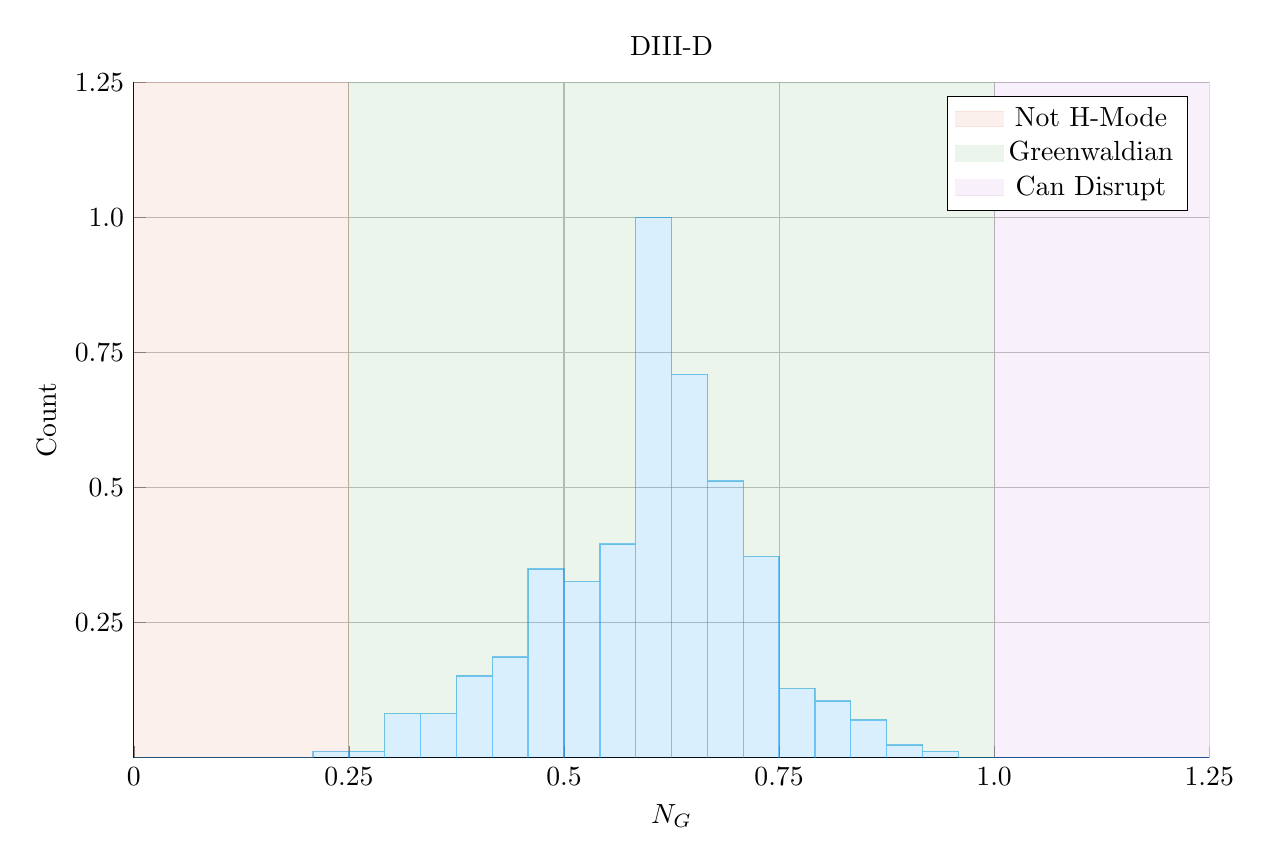
\begin{tikzpicture}[]
\begin{axis}[height = {101.6mm}, ylabel = {Count}, title = {DIII-D}, xmin = {0}, xmax = {1.25}, ymax = {1.25}, xlabel = {$N_G$}, {unbounded coords=jump, scaled x ticks = false, xticklabel style={rotate = 0}, xmajorgrids = true, xtick = {0.0,0.25,0.5,0.75,1.0,1.25}, xticklabels = {0,0.25,0.5,0.75,1.0,1.25}, xtick align = inside, axis lines* = left, scaled y ticks = false, yticklabel style={rotate = 0}, ymajorgrids = true, ytick = {0.0,0.25,0.5,0.75,1.0,1.25}, yticklabels = {,0.25,0.5,0.75,1.0,1.25}, ytick align = inside, axis lines* = left,     xshift = 0.0mm,
    yshift = 0.0mm,
    axis background/.style={fill={rgb,1:red,1.00000000;green,1.00000000;blue,1.00000000}}
}, ymin = {0}, width = {152.4mm}]\addplot+ [color = {rgb,1:red,0.00000000;green,0.60560316;blue,0.97868012},
draw opacity=0.5,
line width=0.5,
solid,mark = none,
mark size = 2.0,
mark options = {
    color = {rgb,1:red,0.00000000;green,0.00000000;blue,0.00000000}, draw opacity = 0.5,
    fill = {rgb,1:red,0.00000000;green,0.60560316;blue,0.97868012}, fill opacity = 0.5,
    line width = 1,
    rotate = 0,
    solid
},fill = {rgb,1:red,0.00000000;green,0.60560316;blue,0.97868012}, fill opacity=0.15,forget plot]coordinates {
(0.0, 0.0)
(0.0, 0.0)
(0.041666666666666664, 0.0)
(0.041666666666666664, 0.0)
(NaN, NaN)
(0.041666666666666664, 0.0)
(0.041666666666666664, 0.0)
(0.08333333333333333, 0.0)
(0.08333333333333333, 0.0)
(NaN, NaN)
(0.08333333333333333, 0.0)
(0.08333333333333333, 0.0)
(0.125, 0.0)
(0.125, 0.0)
(NaN, NaN)
(0.125, 0.0)
(0.125, 0.0)
(0.16666666666666666, 0.0)
(0.16666666666666666, 0.0)
(NaN, NaN)
(0.16666666666666666, 0.0)
(0.16666666666666666, 0.0)
(0.20833333333333334, 0.0)
(0.20833333333333334, 0.0)
(NaN, NaN)
(0.20833333333333334, 0.0)
(0.20833333333333334, 0.011627906976744186)
(0.25, 0.011627906976744186)
(0.25, 0.0)
(NaN, NaN)
(0.25, 0.0)
(0.25, 0.011627906976744186)
(0.2916666666666667, 0.011627906976744186)
(0.2916666666666667, 0.0)
(NaN, NaN)
(0.2916666666666667, 0.0)
(0.2916666666666667, 0.08139534883720931)
(0.3333333333333333, 0.08139534883720931)
(0.3333333333333333, 0.0)
(NaN, NaN)
(0.3333333333333333, 0.0)
(0.3333333333333333, 0.08139534883720931)
(0.375, 0.08139534883720931)
(0.375, 0.0)
(NaN, NaN)
(0.375, 0.0)
(0.375, 0.1511627906976744)
(0.4166666666666667, 0.1511627906976744)
(0.4166666666666667, 0.0)
(NaN, NaN)
(0.4166666666666667, 0.0)
(0.4166666666666667, 0.18604651162790697)
(0.4583333333333333, 0.18604651162790697)
(0.4583333333333333, 0.0)
(NaN, NaN)
(0.4583333333333333, 0.0)
(0.4583333333333333, 0.3488372093023256)
(0.5, 0.3488372093023256)
(0.5, 0.0)
(NaN, NaN)
(0.5, 0.0)
(0.5, 0.32558139534883723)
(0.5416666666666666, 0.32558139534883723)
(0.5416666666666666, 0.0)
(NaN, NaN)
(0.5416666666666666, 0.0)
(0.5416666666666666, 0.3953488372093023)
(0.5833333333333334, 0.3953488372093023)
(0.5833333333333334, 0.0)
(NaN, NaN)
(0.5833333333333334, 0.0)
(0.5833333333333334, 1.0)
(0.625, 1.0)
(0.625, 0.0)
(NaN, NaN)
(0.625, 0.0)
(0.625, 0.7093023255813954)
(0.6666666666666666, 0.7093023255813954)
(0.6666666666666666, 0.0)
(NaN, NaN)
(0.6666666666666666, 0.0)
(0.6666666666666666, 0.5116279069767442)
(0.7083333333333334, 0.5116279069767442)
(0.7083333333333334, 0.0)
(NaN, NaN)
(0.7083333333333334, 0.0)
(0.7083333333333334, 0.37209302325581395)
(0.75, 0.37209302325581395)
(0.75, 0.0)
(NaN, NaN)
(0.75, 0.0)
(0.75, 0.12790697674418605)
(0.7916666666666666, 0.12790697674418605)
(0.7916666666666666, 0.0)
(NaN, NaN)
(0.7916666666666666, 0.0)
(0.7916666666666666, 0.10465116279069768)
(0.8333333333333334, 0.10465116279069768)
(0.8333333333333334, 0.0)
(NaN, NaN)
(0.8333333333333334, 0.0)
(0.8333333333333334, 0.06976744186046512)
(0.875, 0.06976744186046512)
(0.875, 0.0)
(NaN, NaN)
(0.875, 0.0)
(0.875, 0.023255813953488372)
(0.9166666666666666, 0.023255813953488372)
(0.9166666666666666, 0.0)
(NaN, NaN)
(0.9166666666666666, 0.0)
(0.9166666666666666, 0.011627906976744186)
(0.9583333333333334, 0.011627906976744186)
(0.9583333333333334, 0.0)
(NaN, NaN)
(0.9583333333333334, 0.0)
(0.9583333333333334, 0.0)
(1.0, 0.0)
(1.0, 0.0)
(NaN, NaN)
(1.0, 0.0)
(1.0, 0.0)
(1.0416666666666667, 0.0)
(1.0416666666666667, 0.0)
(NaN, NaN)
(1.0416666666666667, 0.0)
(1.0416666666666667, 0.0)
(1.0833333333333333, 0.0)
(1.0833333333333333, 0.0)
(NaN, NaN)
(1.0833333333333333, 0.0)
(1.0833333333333333, 0.0)
(1.125, 0.0)
(1.125, 0.0)
(NaN, NaN)
(1.125, 0.0)
(1.125, 0.0)
(1.1666666666666667, 0.0)
(1.1666666666666667, 0.0)
(NaN, NaN)
(1.1666666666666667, 0.0)
(1.1666666666666667, 0.0)
(1.2083333333333333, 0.0)
(1.2083333333333333, 0.0)
(NaN, NaN)
(1.2083333333333333, 0.0)
(1.2083333333333333, 0.0)
(1.25, 0.0)
(1.25, 0.0)
(NaN, NaN)
};
\addplot+ [color = {rgb,1:red,0.88887350;green,0.43564919;blue,0.27812294},
draw opacity=0.1,
line width=0,
solid,mark = none,
mark size = 2.0,
mark options = {
    color = {rgb,1:red,0.00000000;green,0.00000000;blue,0.00000000}, draw opacity = 0.1,
    fill = {rgb,1:red,0.88887350;green,0.43564919;blue,0.27812294}, fill opacity = 0.1,
    line width = 1,
    rotate = 0,
    solid
},fill = {rgb,1:red,0.88887350;green,0.43564919;blue,0.27812294}, fill opacity=0.1,area legend]coordinates {
(0.0, 1.25)
(0.0, 0.0)
(0.041666666666666664, 0.0)
(0.041666666666666664, 0.0)
(0.08333333333333333, 0.0)
(0.08333333333333333, 0.0)
(0.125, 0.0)
(0.125, 0.0)
(0.16666666666666666, 0.0)
(0.16666666666666666, 0.0)
(0.20833333333333334, 0.0)
(0.20833333333333334, 0.011627906976744186)
(0.25, 0.011627906976744186)
(0.25, 1.25)
(0.0, 1.25)
};
\addlegendentry{Not H-Mode}
\addplot+ [color = {rgb,1:red,0.24222430;green,0.64327509;blue,0.30444865},
draw opacity=0.1,
line width=0,
solid,mark = none,
mark size = 2.0,
mark options = {
    color = {rgb,1:red,0.00000000;green,0.00000000;blue,0.00000000}, draw opacity = 0.1,
    fill = {rgb,1:red,0.24222430;green,0.64327509;blue,0.30444865}, fill opacity = 0.1,
    line width = 1,
    rotate = 0,
    solid
},fill = {rgb,1:red,0.24222430;green,0.64327509;blue,0.30444865}, fill opacity=0.1,area legend]coordinates {
(0.25, 1.25)
(0.25, 0.011627906976744186)
(0.2916666666666667, 0.011627906976744186)
(0.2916666666666667, 0.08139534883720931)
(0.3333333333333333, 0.08139534883720931)
(0.3333333333333333, 0.08139534883720931)
(0.375, 0.08139534883720931)
(0.375, 0.1511627906976744)
(0.4166666666666667, 0.1511627906976744)
(0.4166666666666667, 0.18604651162790697)
(0.4583333333333333, 0.18604651162790697)
(0.4583333333333333, 0.3488372093023256)
(0.5, 0.3488372093023256)
(0.5, 0.32558139534883723)
(0.5416666666666666, 0.32558139534883723)
(0.5416666666666666, 0.3953488372093023)
(0.5833333333333334, 0.3953488372093023)
(0.5833333333333334, 1.0)
(0.625, 1.0)
(0.625, 0.7093023255813954)
(0.6666666666666666, 0.7093023255813954)
(0.6666666666666666, 0.5116279069767442)
(0.7083333333333334, 0.5116279069767442)
(0.7083333333333334, 0.37209302325581395)
(0.75, 0.37209302325581395)
(0.75, 0.12790697674418605)
(0.7916666666666666, 0.12790697674418605)
(0.7916666666666666, 0.10465116279069768)
(0.8333333333333334, 0.10465116279069768)
(0.8333333333333334, 0.06976744186046512)
(0.875, 0.06976744186046512)
(0.875, 0.023255813953488372)
(0.9166666666666666, 0.023255813953488372)
(0.9166666666666666, 0.011627906976744186)
(0.9583333333333334, 0.011627906976744186)
(0.9583333333333334, 0.0)
(1.0, 0.0)
(1.0, 1.25)
(0.25, 1.25)
};
\addlegendentry{Greenwaldian}
\addplot+ [color = {rgb,1:red,0.76444018;green,0.44411178;blue,0.82429754},
draw opacity=0.1,
line width=0,
solid,mark = none,
mark size = 2.0,
mark options = {
    color = {rgb,1:red,0.00000000;green,0.00000000;blue,0.00000000}, draw opacity = 0.1,
    fill = {rgb,1:red,0.76444018;green,0.44411178;blue,0.82429754}, fill opacity = 0.1,
    line width = 1,
    rotate = 0,
    solid
},fill = {rgb,1:red,0.76444018;green,0.44411178;blue,0.82429754}, fill opacity=0.1,area legend]coordinates {
(1.0, 1.25)
(1.0, 0.0)
(1.0416666666666667, 0.0)
(1.0416666666666667, 0.0)
(1.0833333333333333, 0.0)
(1.0833333333333333, 0.0)
(1.125, 0.0)
(1.125, 0.0)
(1.1666666666666667, 0.0)
(1.1666666666666667, 0.0)
(1.2083333333333333, 0.0)
(1.2083333333333333, 0.0)
(1.25, 0.0)
(1.25, 1.25)
(1.0, 1.25)
};
\addlegendentry{Can Disrupt}
\end{axis}

\end{tikzpicture}

		\end{adjustbox}
        \caption{DIII-D}
    \end{subfigure}
    \hfill
    \begin{subfigure}[t]{0.45\textwidth}
        \centering
		\begin{adjustbox}{width=\textwidth}
			\Large
			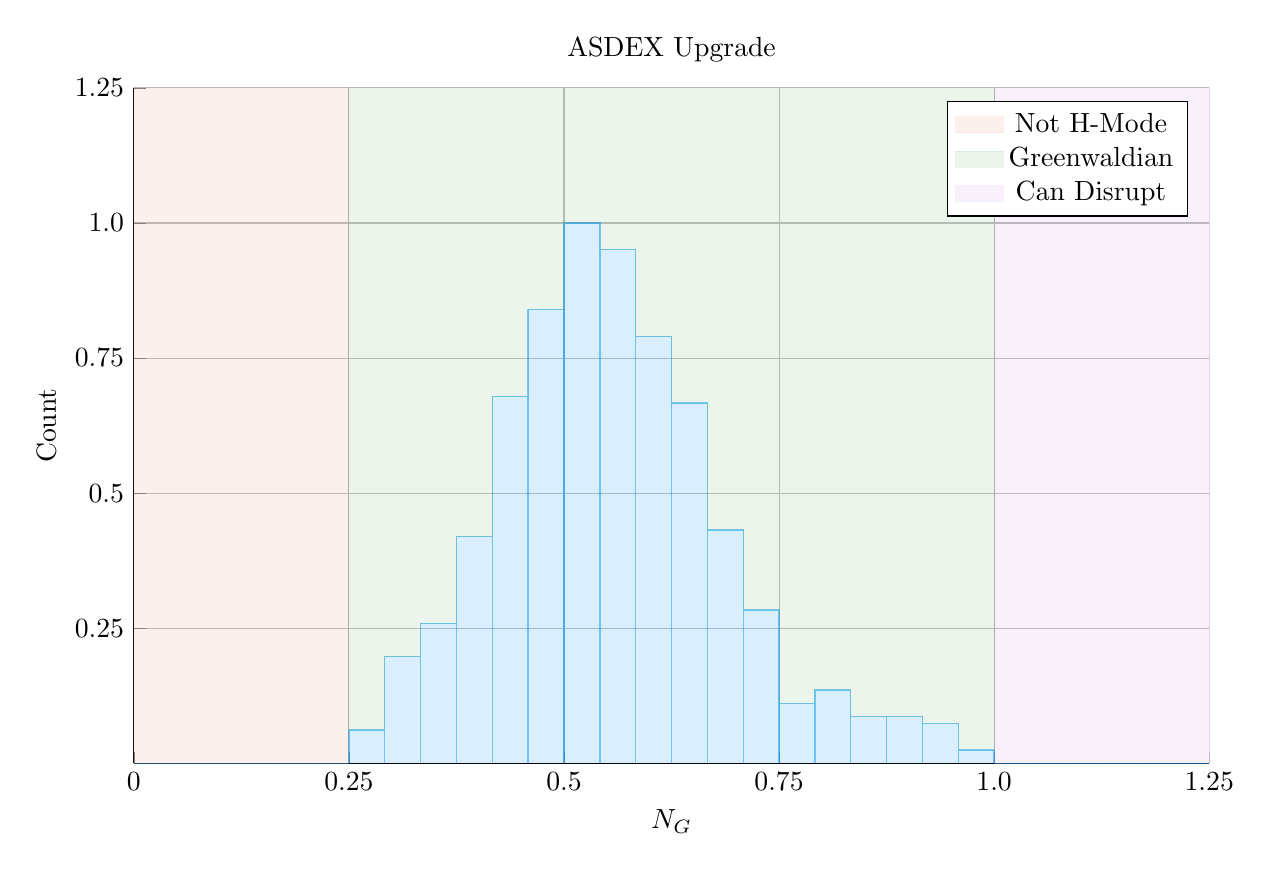
\begin{tikzpicture}[]
\begin{axis}[height = {101.6mm}, ylabel = {Count}, title = {ASDEX Upgrade}, xmin = {0}, xmax = {1.25}, ymax = {1.25}, xlabel = {$N_G$}, {unbounded coords=jump, scaled x ticks = false, xticklabel style={rotate = 0}, xmajorgrids = true, xtick = {0.0,0.25,0.5,0.75,1.0,1.25}, xticklabels = {0,0.25,0.5,0.75,1.0,1.25}, xtick align = inside, axis lines* = left, scaled y ticks = false, yticklabel style={rotate = 0}, ymajorgrids = true, ytick = {0.0,0.25,0.5,0.75,1.0,1.25}, yticklabels = {,0.25,0.5,0.75,1.0,1.25}, ytick align = inside, axis lines* = left,     xshift = 0.0mm,
    yshift = 0.0mm,
    axis background/.style={fill={rgb,1:red,1.00000000;green,1.00000000;blue,1.00000000}}
}, ymin = {0}, width = {152.4mm}]\addplot+ [color = {rgb,1:red,0.00000000;green,0.60560316;blue,0.97868012},
draw opacity=0.5,
line width=0.5,
solid,mark = none,
mark size = 2.0,
mark options = {
    color = {rgb,1:red,0.00000000;green,0.00000000;blue,0.00000000}, draw opacity = 0.5,
    fill = {rgb,1:red,0.00000000;green,0.60560316;blue,0.97868012}, fill opacity = 0.5,
    line width = 1,
    rotate = 0,
    solid
},fill = {rgb,1:red,0.00000000;green,0.60560316;blue,0.97868012}, fill opacity=0.15,forget plot]coordinates {
(0.0, 0.0)
(0.0, 0.0)
(0.041666666666666664, 0.0)
(0.041666666666666664, 0.0)
(NaN, NaN)
(0.041666666666666664, 0.0)
(0.041666666666666664, 0.0)
(0.08333333333333333, 0.0)
(0.08333333333333333, 0.0)
(NaN, NaN)
(0.08333333333333333, 0.0)
(0.08333333333333333, 0.0)
(0.125, 0.0)
(0.125, 0.0)
(NaN, NaN)
(0.125, 0.0)
(0.125, 0.0)
(0.16666666666666666, 0.0)
(0.16666666666666666, 0.0)
(NaN, NaN)
(0.16666666666666666, 0.0)
(0.16666666666666666, 0.0)
(0.20833333333333334, 0.0)
(0.20833333333333334, 0.0)
(NaN, NaN)
(0.20833333333333334, 0.0)
(0.20833333333333334, 0.0)
(0.25, 0.0)
(0.25, 0.0)
(NaN, NaN)
(0.25, 0.0)
(0.25, 0.06172839506172839)
(0.2916666666666667, 0.06172839506172839)
(0.2916666666666667, 0.0)
(NaN, NaN)
(0.2916666666666667, 0.0)
(0.2916666666666667, 0.19753086419753085)
(0.3333333333333333, 0.19753086419753085)
(0.3333333333333333, 0.0)
(NaN, NaN)
(0.3333333333333333, 0.0)
(0.3333333333333333, 0.25925925925925924)
(0.375, 0.25925925925925924)
(0.375, 0.0)
(NaN, NaN)
(0.375, 0.0)
(0.375, 0.41975308641975306)
(0.4166666666666667, 0.41975308641975306)
(0.4166666666666667, 0.0)
(NaN, NaN)
(0.4166666666666667, 0.0)
(0.4166666666666667, 0.6790123456790124)
(0.4583333333333333, 0.6790123456790124)
(0.4583333333333333, 0.0)
(NaN, NaN)
(0.4583333333333333, 0.0)
(0.4583333333333333, 0.8395061728395061)
(0.5, 0.8395061728395061)
(0.5, 0.0)
(NaN, NaN)
(0.5, 0.0)
(0.5, 1.0)
(0.5416666666666666, 1.0)
(0.5416666666666666, 0.0)
(NaN, NaN)
(0.5416666666666666, 0.0)
(0.5416666666666666, 0.9506172839506173)
(0.5833333333333334, 0.9506172839506173)
(0.5833333333333334, 0.0)
(NaN, NaN)
(0.5833333333333334, 0.0)
(0.5833333333333334, 0.7901234567901234)
(0.625, 0.7901234567901234)
(0.625, 0.0)
(NaN, NaN)
(0.625, 0.0)
(0.625, 0.6666666666666666)
(0.6666666666666666, 0.6666666666666666)
(0.6666666666666666, 0.0)
(NaN, NaN)
(0.6666666666666666, 0.0)
(0.6666666666666666, 0.43209876543209874)
(0.7083333333333334, 0.43209876543209874)
(0.7083333333333334, 0.0)
(NaN, NaN)
(0.7083333333333334, 0.0)
(0.7083333333333334, 0.2839506172839506)
(0.75, 0.2839506172839506)
(0.75, 0.0)
(NaN, NaN)
(0.75, 0.0)
(0.75, 0.1111111111111111)
(0.7916666666666666, 0.1111111111111111)
(0.7916666666666666, 0.0)
(NaN, NaN)
(0.7916666666666666, 0.0)
(0.7916666666666666, 0.13580246913580246)
(0.8333333333333334, 0.13580246913580246)
(0.8333333333333334, 0.0)
(NaN, NaN)
(0.8333333333333334, 0.0)
(0.8333333333333334, 0.08641975308641975)
(0.875, 0.08641975308641975)
(0.875, 0.0)
(NaN, NaN)
(0.875, 0.0)
(0.875, 0.08641975308641975)
(0.9166666666666666, 0.08641975308641975)
(0.9166666666666666, 0.0)
(NaN, NaN)
(0.9166666666666666, 0.0)
(0.9166666666666666, 0.07407407407407407)
(0.9583333333333334, 0.07407407407407407)
(0.9583333333333334, 0.0)
(NaN, NaN)
(0.9583333333333334, 0.0)
(0.9583333333333334, 0.024691358024691357)
(1.0, 0.024691358024691357)
(1.0, 0.0)
(NaN, NaN)
(1.0, 0.0)
(1.0, 0.0)
(1.0416666666666667, 0.0)
(1.0416666666666667, 0.0)
(NaN, NaN)
(1.0416666666666667, 0.0)
(1.0416666666666667, 0.0)
(1.0833333333333333, 0.0)
(1.0833333333333333, 0.0)
(NaN, NaN)
(1.0833333333333333, 0.0)
(1.0833333333333333, 0.0)
(1.125, 0.0)
(1.125, 0.0)
(NaN, NaN)
(1.125, 0.0)
(1.125, 0.0)
(1.1666666666666667, 0.0)
(1.1666666666666667, 0.0)
(NaN, NaN)
(1.1666666666666667, 0.0)
(1.1666666666666667, 0.0)
(1.2083333333333333, 0.0)
(1.2083333333333333, 0.0)
(NaN, NaN)
(1.2083333333333333, 0.0)
(1.2083333333333333, 0.0)
(1.25, 0.0)
(1.25, 0.0)
(NaN, NaN)
};
\addplot+ [color = {rgb,1:red,0.88887350;green,0.43564919;blue,0.27812294},
draw opacity=0.1,
line width=0,
solid,mark = none,
mark size = 2.0,
mark options = {
    color = {rgb,1:red,0.00000000;green,0.00000000;blue,0.00000000}, draw opacity = 0.1,
    fill = {rgb,1:red,0.88887350;green,0.43564919;blue,0.27812294}, fill opacity = 0.1,
    line width = 1,
    rotate = 0,
    solid
},fill = {rgb,1:red,0.88887350;green,0.43564919;blue,0.27812294}, fill opacity=0.1,area legend]coordinates {
(0.0, 1.25)
(0.0, 0.0)
(0.041666666666666664, 0.0)
(0.041666666666666664, 0.0)
(0.08333333333333333, 0.0)
(0.08333333333333333, 0.0)
(0.125, 0.0)
(0.125, 0.0)
(0.16666666666666666, 0.0)
(0.16666666666666666, 0.0)
(0.20833333333333334, 0.0)
(0.20833333333333334, 0.0)
(0.25, 0.0)
(0.25, 1.25)
(0.0, 1.25)
};
\addlegendentry{Not H-Mode}
\addplot+ [color = {rgb,1:red,0.24222430;green,0.64327509;blue,0.30444865},
draw opacity=0.1,
line width=0,
solid,mark = none,
mark size = 2.0,
mark options = {
    color = {rgb,1:red,0.00000000;green,0.00000000;blue,0.00000000}, draw opacity = 0.1,
    fill = {rgb,1:red,0.24222430;green,0.64327509;blue,0.30444865}, fill opacity = 0.1,
    line width = 1,
    rotate = 0,
    solid
},fill = {rgb,1:red,0.24222430;green,0.64327509;blue,0.30444865}, fill opacity=0.1,area legend]coordinates {
(0.25, 1.25)
(0.25, 0.06172839506172839)
(0.2916666666666667, 0.06172839506172839)
(0.2916666666666667, 0.19753086419753085)
(0.3333333333333333, 0.19753086419753085)
(0.3333333333333333, 0.25925925925925924)
(0.375, 0.25925925925925924)
(0.375, 0.41975308641975306)
(0.4166666666666667, 0.41975308641975306)
(0.4166666666666667, 0.6790123456790124)
(0.4583333333333333, 0.6790123456790124)
(0.4583333333333333, 0.8395061728395061)
(0.5, 0.8395061728395061)
(0.5, 1.0)
(0.5416666666666666, 1.0)
(0.5416666666666666, 0.9506172839506173)
(0.5833333333333334, 0.9506172839506173)
(0.5833333333333334, 0.7901234567901234)
(0.625, 0.7901234567901234)
(0.625, 0.6666666666666666)
(0.6666666666666666, 0.6666666666666666)
(0.6666666666666666, 0.43209876543209874)
(0.7083333333333334, 0.43209876543209874)
(0.7083333333333334, 0.2839506172839506)
(0.75, 0.2839506172839506)
(0.75, 0.1111111111111111)
(0.7916666666666666, 0.1111111111111111)
(0.7916666666666666, 0.13580246913580246)
(0.8333333333333334, 0.13580246913580246)
(0.8333333333333334, 0.08641975308641975)
(0.875, 0.08641975308641975)
(0.875, 0.08641975308641975)
(0.9166666666666666, 0.08641975308641975)
(0.9166666666666666, 0.07407407407407407)
(0.9583333333333334, 0.07407407407407407)
(0.9583333333333334, 0.024691358024691357)
(1.0, 0.024691358024691357)
(1.0, 1.25)
(0.25, 1.25)
};
\addlegendentry{Greenwaldian}
\addplot+ [color = {rgb,1:red,0.76444018;green,0.44411178;blue,0.82429754},
draw opacity=0.1,
line width=0,
solid,mark = none,
mark size = 2.0,
mark options = {
    color = {rgb,1:red,0.00000000;green,0.00000000;blue,0.00000000}, draw opacity = 0.1,
    fill = {rgb,1:red,0.76444018;green,0.44411178;blue,0.82429754}, fill opacity = 0.1,
    line width = 1,
    rotate = 0,
    solid
},fill = {rgb,1:red,0.76444018;green,0.44411178;blue,0.82429754}, fill opacity=0.1,area legend]coordinates {
(1.0, 1.25)
(1.0, 0.0)
(1.0416666666666667, 0.0)
(1.0416666666666667, 0.0)
(1.0833333333333333, 0.0)
(1.0833333333333333, 0.0)
(1.125, 0.0)
(1.125, 0.0)
(1.1666666666666667, 0.0)
(1.1666666666666667, 0.0)
(1.2083333333333333, 0.0)
(1.2083333333333333, 0.0)
(1.25, 0.0)
(1.25, 1.25)
(1.0, 1.25)
};
\addlegendentry{Can Disrupt}
\end{axis}

\end{tikzpicture}

		\end{adjustbox}
        \caption{ASDEX}
    \end{subfigure}
    \hfill \hfill ~\\ ~\\ ~\\
    \begin{subfigure}[t]{0.6\textwidth}
        \centering
		\begin{adjustbox}{width=\textwidth}
			\large
			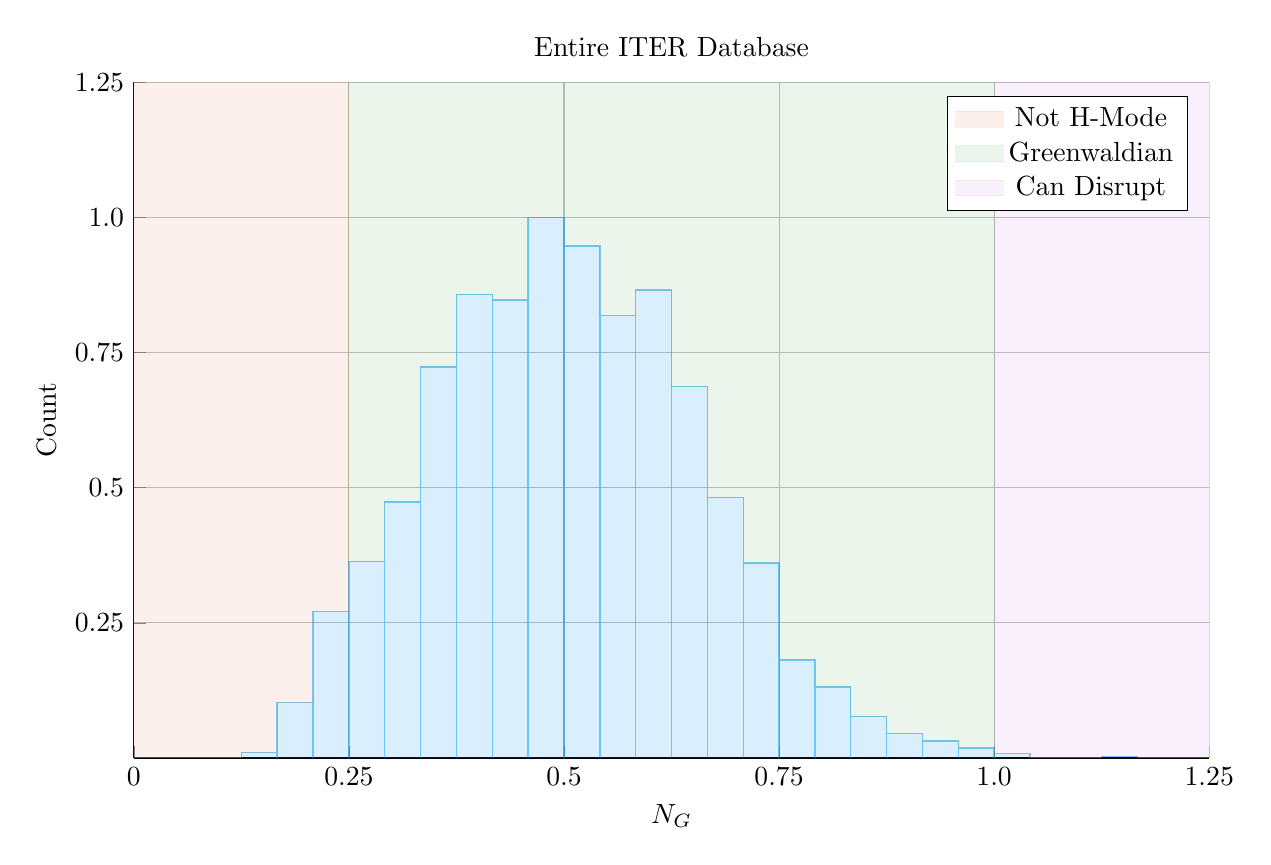
\begin{tikzpicture}[]
\begin{axis}[height = {101.6mm}, ylabel = {Count}, title = {Entire ITER Database}, xmin = {0}, xmax = {1.25}, ymax = {1.25}, xlabel = {$N_G$}, {unbounded coords=jump, scaled x ticks = false, xticklabel style={rotate = 0}, xmajorgrids = true, xtick = {0.0,0.25,0.5,0.75,1.0,1.25}, xticklabels = {0,0.25,0.5,0.75,1.0,1.25}, xtick align = inside, axis lines* = left, scaled y ticks = false, yticklabel style={rotate = 0}, ymajorgrids = true, ytick = {0.0,0.25,0.5,0.75,1.0,1.25}, yticklabels = {,0.25,0.5,0.75,1.0,1.25}, ytick align = inside, axis lines* = left,     xshift = 0.0mm,
    yshift = 0.0mm,
    axis background/.style={fill={rgb,1:red,1.00000000;green,1.00000000;blue,1.00000000}}
}, ymin = {0}, width = {152.4mm}]\addplot+ [color = {rgb,1:red,0.00000000;green,0.60560316;blue,0.97868012},
draw opacity=0.5,
line width=0.5,
solid,mark = none,
mark size = 2.0,
mark options = {
    color = {rgb,1:red,0.00000000;green,0.00000000;blue,0.00000000}, draw opacity = 0.5,
    fill = {rgb,1:red,0.00000000;green,0.60560316;blue,0.97868012}, fill opacity = 0.5,
    line width = 1,
    rotate = 0,
    solid
},fill = {rgb,1:red,0.00000000;green,0.60560316;blue,0.97868012}, fill opacity=0.15,forget plot]coordinates {
(0.0, 0.0)
(0.0, 0.0)
(0.041666666666666664, 0.0)
(0.041666666666666664, 0.0)
(NaN, NaN)
(0.041666666666666664, 0.0)
(0.041666666666666664, 0.0)
(0.08333333333333333, 0.0)
(0.08333333333333333, 0.0)
(NaN, NaN)
(0.08333333333333333, 0.0)
(0.08333333333333333, 0.0)
(0.125, 0.0)
(0.125, 0.0)
(NaN, NaN)
(0.125, 0.0)
(0.125, 0.010526315789473684)
(0.16666666666666666, 0.010526315789473684)
(0.16666666666666666, 0.0)
(NaN, NaN)
(0.16666666666666666, 0.0)
(0.16666666666666666, 0.10263157894736842)
(0.20833333333333334, 0.10263157894736842)
(0.20833333333333334, 0.0)
(NaN, NaN)
(0.20833333333333334, 0.0)
(0.20833333333333334, 0.2710526315789474)
(0.25, 0.2710526315789474)
(0.25, 0.0)
(NaN, NaN)
(0.25, 0.0)
(0.25, 0.3631578947368421)
(0.2916666666666667, 0.3631578947368421)
(0.2916666666666667, 0.0)
(NaN, NaN)
(0.2916666666666667, 0.0)
(0.2916666666666667, 0.47368421052631576)
(0.3333333333333333, 0.47368421052631576)
(0.3333333333333333, 0.0)
(NaN, NaN)
(0.3333333333333333, 0.0)
(0.3333333333333333, 0.7236842105263158)
(0.375, 0.7236842105263158)
(0.375, 0.0)
(NaN, NaN)
(0.375, 0.0)
(0.375, 0.8578947368421053)
(0.4166666666666667, 0.8578947368421053)
(0.4166666666666667, 0.0)
(NaN, NaN)
(0.4166666666666667, 0.0)
(0.4166666666666667, 0.8473684210526315)
(0.4583333333333333, 0.8473684210526315)
(0.4583333333333333, 0.0)
(NaN, NaN)
(0.4583333333333333, 0.0)
(0.4583333333333333, 1.0)
(0.5, 1.0)
(0.5, 0.0)
(NaN, NaN)
(0.5, 0.0)
(0.5, 0.9473684210526315)
(0.5416666666666666, 0.9473684210526315)
(0.5416666666666666, 0.0)
(NaN, NaN)
(0.5416666666666666, 0.0)
(0.5416666666666666, 0.8184210526315789)
(0.5833333333333334, 0.8184210526315789)
(0.5833333333333334, 0.0)
(NaN, NaN)
(0.5833333333333334, 0.0)
(0.5833333333333334, 0.8657894736842106)
(0.625, 0.8657894736842106)
(0.625, 0.0)
(NaN, NaN)
(0.625, 0.0)
(0.625, 0.6868421052631579)
(0.6666666666666666, 0.6868421052631579)
(0.6666666666666666, 0.0)
(NaN, NaN)
(0.6666666666666666, 0.0)
(0.6666666666666666, 0.48157894736842105)
(0.7083333333333334, 0.48157894736842105)
(0.7083333333333334, 0.0)
(NaN, NaN)
(0.7083333333333334, 0.0)
(0.7083333333333334, 0.3605263157894737)
(0.75, 0.3605263157894737)
(0.75, 0.0)
(NaN, NaN)
(0.75, 0.0)
(0.75, 0.18157894736842106)
(0.7916666666666666, 0.18157894736842106)
(0.7916666666666666, 0.0)
(NaN, NaN)
(0.7916666666666666, 0.0)
(0.7916666666666666, 0.13157894736842105)
(0.8333333333333334, 0.13157894736842105)
(0.8333333333333334, 0.0)
(NaN, NaN)
(0.8333333333333334, 0.0)
(0.8333333333333334, 0.07631578947368421)
(0.875, 0.07631578947368421)
(0.875, 0.0)
(NaN, NaN)
(0.875, 0.0)
(0.875, 0.04473684210526316)
(0.9166666666666666, 0.04473684210526316)
(0.9166666666666666, 0.0)
(NaN, NaN)
(0.9166666666666666, 0.0)
(0.9166666666666666, 0.031578947368421054)
(0.9583333333333334, 0.031578947368421054)
(0.9583333333333334, 0.0)
(NaN, NaN)
(0.9583333333333334, 0.0)
(0.9583333333333334, 0.018421052631578946)
(1.0, 0.018421052631578946)
(1.0, 0.0)
(NaN, NaN)
(1.0, 0.0)
(1.0, 0.007894736842105263)
(1.0416666666666667, 0.007894736842105263)
(1.0416666666666667, 0.0)
(NaN, NaN)
(1.0416666666666667, 0.0)
(1.0416666666666667, 0.0)
(1.0833333333333333, 0.0)
(1.0833333333333333, 0.0)
(NaN, NaN)
(1.0833333333333333, 0.0)
(1.0833333333333333, 0.0)
(1.125, 0.0)
(1.125, 0.0)
(NaN, NaN)
(1.125, 0.0)
(1.125, 0.002631578947368421)
(1.1666666666666667, 0.002631578947368421)
(1.1666666666666667, 0.0)
(NaN, NaN)
(1.1666666666666667, 0.0)
(1.1666666666666667, 0.0)
(1.2083333333333333, 0.0)
(1.2083333333333333, 0.0)
(NaN, NaN)
(1.2083333333333333, 0.0)
(1.2083333333333333, 0.0)
(1.25, 0.0)
(1.25, 0.0)
(NaN, NaN)
};
\addplot+ [color = {rgb,1:red,0.88887350;green,0.43564919;blue,0.27812294},
draw opacity=0.1,
line width=0,
solid,mark = none,
mark size = 2.0,
mark options = {
    color = {rgb,1:red,0.00000000;green,0.00000000;blue,0.00000000}, draw opacity = 0.1,
    fill = {rgb,1:red,0.88887350;green,0.43564919;blue,0.27812294}, fill opacity = 0.1,
    line width = 1,
    rotate = 0,
    solid
},fill = {rgb,1:red,0.88887350;green,0.43564919;blue,0.27812294}, fill opacity=0.1,area legend]coordinates {
(0.0, 1.25)
(0.0, 0.0)
(0.041666666666666664, 0.0)
(0.041666666666666664, 0.0)
(0.08333333333333333, 0.0)
(0.08333333333333333, 0.0)
(0.125, 0.0)
(0.125, 0.010526315789473684)
(0.16666666666666666, 0.010526315789473684)
(0.16666666666666666, 0.10263157894736842)
(0.20833333333333334, 0.10263157894736842)
(0.20833333333333334, 0.2710526315789474)
(0.25, 0.2710526315789474)
(0.25, 1.25)
(0.0, 1.25)
};
\addlegendentry{Not H-Mode}
\addplot+ [color = {rgb,1:red,0.24222430;green,0.64327509;blue,0.30444865},
draw opacity=0.1,
line width=0,
solid,mark = none,
mark size = 2.0,
mark options = {
    color = {rgb,1:red,0.00000000;green,0.00000000;blue,0.00000000}, draw opacity = 0.1,
    fill = {rgb,1:red,0.24222430;green,0.64327509;blue,0.30444865}, fill opacity = 0.1,
    line width = 1,
    rotate = 0,
    solid
},fill = {rgb,1:red,0.24222430;green,0.64327509;blue,0.30444865}, fill opacity=0.1,area legend]coordinates {
(0.25, 1.25)
(0.25, 0.3631578947368421)
(0.2916666666666667, 0.3631578947368421)
(0.2916666666666667, 0.47368421052631576)
(0.3333333333333333, 0.47368421052631576)
(0.3333333333333333, 0.7236842105263158)
(0.375, 0.7236842105263158)
(0.375, 0.8578947368421053)
(0.4166666666666667, 0.8578947368421053)
(0.4166666666666667, 0.8473684210526315)
(0.4583333333333333, 0.8473684210526315)
(0.4583333333333333, 1.0)
(0.5, 1.0)
(0.5, 0.9473684210526315)
(0.5416666666666666, 0.9473684210526315)
(0.5416666666666666, 0.8184210526315789)
(0.5833333333333334, 0.8184210526315789)
(0.5833333333333334, 0.8657894736842106)
(0.625, 0.8657894736842106)
(0.625, 0.6868421052631579)
(0.6666666666666666, 0.6868421052631579)
(0.6666666666666666, 0.48157894736842105)
(0.7083333333333334, 0.48157894736842105)
(0.7083333333333334, 0.3605263157894737)
(0.75, 0.3605263157894737)
(0.75, 0.18157894736842106)
(0.7916666666666666, 0.18157894736842106)
(0.7916666666666666, 0.13157894736842105)
(0.8333333333333334, 0.13157894736842105)
(0.8333333333333334, 0.07631578947368421)
(0.875, 0.07631578947368421)
(0.875, 0.04473684210526316)
(0.9166666666666666, 0.04473684210526316)
(0.9166666666666666, 0.031578947368421054)
(0.9583333333333334, 0.031578947368421054)
(0.9583333333333334, 0.018421052631578946)
(1.0, 0.018421052631578946)
(1.0, 1.25)
(0.25, 1.25)
};
\addlegendentry{Greenwaldian}
\addplot+ [color = {rgb,1:red,0.76444018;green,0.44411178;blue,0.82429754},
draw opacity=0.1,
line width=0,
solid,mark = none,
mark size = 2.0,
mark options = {
    color = {rgb,1:red,0.00000000;green,0.00000000;blue,0.00000000}, draw opacity = 0.1,
    fill = {rgb,1:red,0.76444018;green,0.44411178;blue,0.82429754}, fill opacity = 0.1,
    line width = 1,
    rotate = 0,
    solid
},fill = {rgb,1:red,0.76444018;green,0.44411178;blue,0.82429754}, fill opacity=0.1,area legend]coordinates {
(1.0, 1.25)
(1.0, 0.007894736842105263)
(1.0416666666666667, 0.007894736842105263)
(1.0416666666666667, 0.0)
(1.0833333333333333, 0.0)
(1.0833333333333333, 0.0)
(1.125, 0.0)
(1.125, 0.002631578947368421)
(1.1666666666666667, 0.002631578947368421)
(1.1666666666666667, 0.0)
(1.2083333333333333, 0.0)
(1.2083333333333333, 0.0)
(1.25, 0.0)
(1.25, 1.25)
(1.0, 1.25)
};
\addlegendentry{Can Disrupt}
\end{axis}

\end{tikzpicture}

		\end{adjustbox}
        \caption{All Tokamak Shots}
    \end{subfigure} ~\\ ~\\ ~\\
    \caption{Greenwald Density Limit} ~\\
    \small The Greenwald Density Limit is a robust metric of what densities an H-Mode plasma can attain. Although empirical in nature, \replaced{it accurately predicts when a tokamak will undergo degraded plasma transport.\cite{greenwald}}{it is an indicator for good transport regimes.}
    \label{fig:greenwald}
\end{figure*}

As no theoretical backing exists, the Greenwald density limit can simply be written (with citation) as: \cite{greenwald}
\begin{equation}
	\hat n = N_G \cdot \left( \frac{ I_P }{ \pi a^2} \right)
\end{equation}
Here, $\hat n$ has units of $10^{20} \ \frac{\textnormal{particles}}{\textnormal{m}^3}$, $N_G$ is the Greenwald density fraction, \added{and} $I_P$ is again the plasma current (measured in mega-amps)\added{.} \deleted{ and $\pi$ has its usual meaning(3.141592653...).} The final variable is then the minor radius -- a -- which was previously defined through:
\begin{equation}
	\tag{\ref{eq:a}}
	a = \epsilon \cdot R_0
\end{equation}
The next step is transforming the \emph{line-averaged} density ($\hat n$) into the \emph{volume-averaged} version ($\overline n$) used in this model. Harnessing the simplicity of the density's parabolic profile allows this relation to be written in a closed form as:
 \begin{equation}
 	\hat n = \frac{\sqrt{\pi}}{2} \cdot \left( \frac{\Gamma \left( \nu_n + 2 \right)}{\Gamma \left( \nu_n + \frac{3}{2} \right)} \right) \cdot \overline n 
 \end{equation}
 
 Where $\Gamma( \, \cdots)$ represents the gamma function: the non-integer analogue of the factorial function.
 
 Combining these pieces allows the volume-averaged density to be written in standardized units \deleted{(i.e.\ the ones we use)} as:
 \begin{equation}
 	\label{eq:greenwald}
 	\tcbhighmath{
 	\overline n = K_n \cdot \left( \frac{I_P}{R_0^2} \right)
 	}
 \end{equation}
 \myequations{Greenwald Density -- $\overline n$}
 \begin{equation}
 	K_n = \frac{2 N_G}{\epsilon^2 \, \pi^{3/2} } \cdot \left( \frac{\Gamma \left( \nu_n + \frac{3}{2} \right)}{\Gamma \left( \nu_n + 2 \right)} \right)
\end{equation}
The format of the previous equation pair will be used throughout the remainder of the paper. The top equation relates \replaced{dynamic}{floating} variables (i.e.\ $\overline n$, $I_P$, and $R_0$), while the \replaced{static}{fixed}-value coefficient ($K_n$) lumps together \replaced{static}{fixed} quantities, such as: $N_G$, $\epsilon$, 2, $\pi$, and $\nu_n$.

\subsection{Declaring the Bootstrap Current}

The first term to define in current balance, \cref{eq:ibal}, is the bootstrap current. This bootstrap current is a mechanism of tokamak plasmas that helps supply some of the current needed to keep a plasma \replaced{in equilibrium}{stable}. \replaced{Its underlying behavior stems from particles stuck in banana-shaped orbits on the outer edges of the device propelling the majority species along their helical trajectories around the tokamak.
}{From a hand-waving perspective, it involves particles stuck in banana-shaped orbits on the outer edges of a tokamak behaving like racing-game style speed boosts that accelerate charged particles along their hooped-shaped race tracks.}

\replaced{Utilizing the surface integral from \cref{eq:qs}, the bootstrap current ($I_{BS}$) can be written in terms of the temperature and density profiles:
}{To get an equation for bootstrap current, we must first introduce the surface integral -- made possible from our previous choice of geometric parameters:
}

%\begin{equation}
%	\tag{\ref{eq:qs}}
%	Q_S = 2 \pi a^2 \kappa g \int_0^1 Q(\rho) \rho \, d\rho
%\end{equation}
%\myequations{Surface Integral -- $Q_S$}

\deleted{Here, Q is an arbitrary function of the normalized radius ($\rho$) and g is a geometric factor (of order 1):}

%\begin{equation}
%	g = \frac{1}{8} \cdot \left( 9 - 2 \delta - 0.3 \left( 1 - \delta^2 \right)  \right)
%\end{equation}

 \deleted{This allows the bootstrap current ($I_{BS}$) to be written in terms of the temperature and density profiles:}
\begin{equation}
	I_{BS} = 2 \pi a^2 \kappa g \int_0^1 J_{BS} \, \rho \, d\rho
\end{equation}
\begin{equation}
\begin{split}
	J_{BS} & = f\left( n , T , \frac{dn}{d\rho} , \frac{dT}{d\rho}  \right) \\
		& \equiv -4.85 \cdot n \cdot T \cdot \frac{ R_0 \sqrt{ \epsilon \, \rho } }{ \sfrac{d\psi}{d\rho} } \cdot \left( \frac{1}{n} \frac{dn}{d\rho} + 0.54 \, \frac{1}{T} \frac{dT}{d\rho} \right) 
\end{split}
\end{equation}
 \added{
 The second definition for the bootstrap current density -- $J_{BS}$ -- comes from using well known theoretical results plus several simplifying assumptions, including the large aspect limit. The value of $\sfrac{d\psi}{d\rho}$ is given in \cref{chapter:bootstrap}.
 }
 
\deleted{For a more formal look into this $J_{BS}$ function, check the appendix section on pedestal temperatures. The point to make now is that it depends on the the profiles' derivatives, leading to one major discrepancy in the model.}

As shown later in the results, bootstrap fractions are often under-predicted by this model. This is due to parabolic profiles (i.e.\ for temperature) having much less steep declines near the edge (i.e.\ in their derivatives) than characteristic H-Mode profiles with pedestals. This implies that the area most positively impacted by a pedestal profile for temperature would be the bootstrap current derivation. \added{The instructions to do so are given in \cref{section:pedestalbootstrap}. }

\deleted{Getting back on track -- and without completeness -- the bootstrap current can now be written in proportionality form as:}

%\begin{equation}
%	I_{BS} \propto \overline T \cdot \overline n \cdot \left( \frac{R_0^2}{I_P} \right)
%\end{equation}

\deleted{Recognizing that the last term is basically the inverse of the Greenwald density (see Eq. \ref{eq:greenwald}), allows the proportionality to be written in the following form. Note that this implies the bootstrap current is only a function of temperature!}

%\begin{equation}
%	I_{BS} \propto K_n \cdot \overline T
%\end{equation}

\deleted{In standardized units, this proportionality can be written as a concrete relation of the form:}

\added{Finally, summarizing the results of \cref{chapter:bootstrap}, the bootstrap current is found to be only a function of temperature and static variables! In standardized units, it can be written as:}
\begin{equation}
	\label{eq:ibs}
	\tcboxmath{
	I_{BS} = K_{BS} \cdot \overline T
	}
\end{equation}
\myequations{Bootstrap Current -- $I_{BS}$}
\begin{equation}
  K_{BS} = 4.879 \cdot  K_n \cdot \left( \, \frac{1+\kappa^2}{2} \, \right) \cdot \epsilon^{5/2} \cdot H_{BS}
\end{equation}
\begin{equation}
  H_{BS} = ( 1 + \nu_n ) ( 1 + \nu_T ) ( \nu_n + 0.054 \nu_T ) \int_0^1 \frac{ \rho^{\,5/2} \, ( \, 1 - \rho^{\,2} \, )^{\, \nu_n + \nu_T - 1} }{b_p} \, d\rho
\end{equation}
Quickly noting, this $H_{BS}$ term serves as the analogue of \replaced{static}{fixed}-value coefficients (e.g.\ $K_{BS}$ and $K_n$) when they contain an integral. And $b_p$ represents the poloidal magnet strength given by Eq. \ref{eq:b_p}.

\subsection{Deriving the Fusion Power}

\label{subsection:fusion_derive}

\deleted{The next segue on our journey to solving for the steady current is deriving the fusion power ($P_F$), which appears in current drive. This requires a more first-principles approach than those used up until now. As such, a quick background is given to motivate the parameters it adds -- i.e.\ the dilution factor ($f_{D}$) and the Bosch-Hale fusion reactivity ($\sigma v$).}

%\begin{figure}
%	\centering
%	\begin{adjustbox}{width=0.75\textwidth}
%		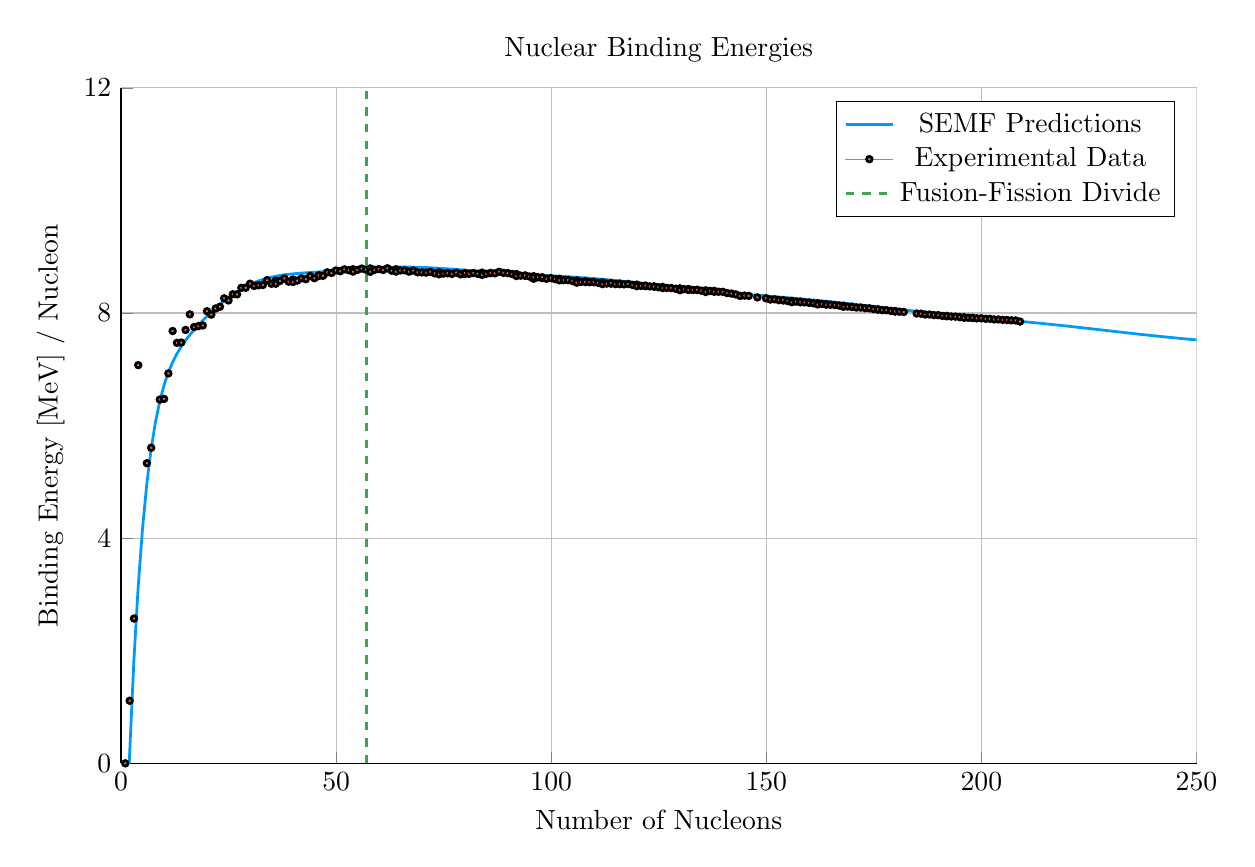
\begin{tikzpicture}[]
\begin{axis}[height = {101.6mm}, ylabel = {Binding Energy [MeV] / Nucleon}, title = {Nuclear Binding Energies}, xmin = {0}, xmax = {250}, ymax = {12}, xlabel = {Number of Nucleons}, {unbounded coords=jump, scaled x ticks = false, xticklabel style={rotate = 0}, xmajorgrids = true, xtick = {0.0,50.0,100.0,150.0,200.0,250.0}, xticklabels = {0,50,100,150,200,250}, xtick align = inside, axis lines* = left, scaled y ticks = false, yticklabel style={rotate = 0}, ymajorgrids = true, ytick = {0.0,4.0,8.0,12.0}, yticklabels = {0,4,8,12}, ytick align = inside, axis lines* = left,     xshift = 0.0mm,
    yshift = 0.0mm,
    axis background/.style={fill={rgb,1:red,1.00000000;green,1.00000000;blue,1.00000000}}
}, ymin = {0}, width = {152.4mm}]\addplot+ [color = {rgb,1:red,0.00000000;green,0.60560316;blue,0.97868012},
draw opacity=1.0,
line width=1,
solid,mark = none,
mark size = 2.0,
mark options = {
    color = {rgb,1:red,0.00000000;green,0.00000000;blue,0.00000000}, draw opacity = 1.0,
    fill = {rgb,1:red,0.00000000;green,0.60560316;blue,0.97868012}, fill opacity = 1.0,
    line width = 1,
    rotate = 0,
    solid
}]coordinates {
(0.0, -4.60355222317376)
(1.0, -1.9423714030316184)
(2.0, 0.17174117296689762)
(3.0, 1.84096399661781)
(4.0, 3.151140198415331)
(5.0, 4.173923283645508)
(6.0, 4.968707102167827)
(7.0, 5.58435286219236)
(8.0, 6.060726579422419)
(9.0, 6.430060629330575)
(10.0, 6.718153095546762)
(11.0, 6.9454184281365565)
(12.0, 7.127802582683796)
(13.0, 7.277575339898747)
(14.0, 7.404011936438574)
(15.0, 7.513975496904414)
(16.0, 7.6124110668622125)
(17.0, 7.702761326082542)
(18.0, 7.78731332582606)
(19.0, 7.867484857048368)
(20.0, 7.94405832862659)
(21.0, 8.017369324812918)
(22.0, 8.087456325980316)
(23.0, 8.154177421651507)
(24.0, 8.217299223743723)
(25.0, 8.276562603700583)
(26.0, 8.331729331502007)
(27.0, 8.382613188387339)
(28.0, 8.429098658726296)
(29.0, 8.471149879476823)
(30.0, 8.508812137244952)
(31.0, 8.542207851888847)
(32.0, 8.571528670372789)
(33.0, 8.59702501341144)
(34.0, 8.618994168442093)
(35.0, 8.637767803574754)
(36.0, 8.653699586296018)
(37.0, 8.66715342570664)
(38.0, 8.678492715810727)
(39.0, 8.688070837773061)
(40.0, 8.696223079017631)
(41.0, 8.703260044649955)
(42.0, 8.709462569971606)
(43.0, 8.715078090099894)
(44.0, 8.720318382160027)
(45.0, 8.725358565619327)
(46.0, 8.730337225625941)
(47.0, 8.735357511312394)
(48.0, 8.74048905473126)
(49.0, 8.745770555203375)
(50.0, 8.75121287745749)
(51.0, 8.756802519009028)
(52.0, 8.762505312039806)
(53.0, 8.76827023680805)
(54.0, 8.774033236747258)
(55.0, 8.779720939428142)
(56.0, 8.785254201806225)
(57.0, 8.790551412530785)
(58.0, 8.795531497975329)
(59.0, 8.800116592037245)
(60.0, 8.804234342184401)
(61.0, 8.80781983582066)
(62.0, 8.810817141406119)
(63.0, 8.813180468193043)
(64.0, 8.814874956307978)
(65.0, 8.815877115972366)
(66.0, 8.816174940266126)
(67.0, 8.815767720260371)
(68.0, 8.814665595039155)
(69.0, 8.81288887100591)
(70.0, 8.810467147004726)
(71.0, 8.807438281492448)
(72.0, 8.803847238531759)
(73.0, 8.799744847854736)
(74.0, 8.795186513048279)
(75.0, 8.790230899697235)
(76.0, 8.78493863297573)
(77.0, 8.77937103143497)
(78.0, 8.773588900376659)
(79.0, 8.767651405642294)
(80.0, 8.76161504469066)
(81.0, 8.755532729350353)
(82.0, 8.749452990095264)
(83.0, 8.743419310368836)
(84.0, 8.737469594886402)
(85.0, 8.731635772840807)
(86.0, 8.725943537136203)
(87.0, 8.72041221331207)
(88.0, 8.71505475533288)
(89.0, 8.709877858732526)
(90.0, 8.704882183589692)
(91.0, 8.700062675015097)
(92.0, 8.695408972428076)
(93.0, 8.690905892370129)
(94.0, 8.686533974543913)
(95.0, 8.682270076666686)
(96.0, 8.678088004492896)
(97.0, 8.67395916751817)
(98.0, 8.669853242580963)
(99.0, 8.665738837927783)
(100.0, 8.661584144823571)
(101.0, 8.657357563363785)
(102.0, 8.65302830389561)
(103.0, 8.648566937275728)
(104.0, 8.643945904303443)
(105.0, 8.639139972215713)
(106.0, 8.634126623930722)
(107.0, 8.628886396202454)
(108.0, 8.623403143699367)
(109.0, 8.617664241985338)
(110.0, 8.611660722384958)
(111.0, 8.605387333426602)
(112.0, 8.598842559648038)
(113.0, 8.592028549789976)
(114.0, 8.58495101272171)
(115.0, 8.57761904583371)
(116.0, 8.570044915671591)
(117.0, 8.562243798972087)
(118.0, 8.554233483777885)
(119.0, 8.546034047126547)
(120.0, 8.537667484888594)
(121.0, 8.52915735205801)
(122.0, 8.520528366411522)
(123.0, 8.511806023276883)
(124.0, 8.503016188183416)
(125.0, 8.494184739476726)
(126.0, 8.48533715574106)
(127.0, 8.476498181446992)
(128.0, 8.467691475241981)
(129.0, 8.458939312854039)
(130.0, 8.450262302915618)
(131.0, 8.441679114253642)
(132.0, 8.433206278428624)
(133.0, 8.424858004233645)
(134.0, 8.416646056664081)
(135.0, 8.408579640871974)
(136.0, 8.40066533194409)
(137.0, 8.392907065338754)
(138.0, 8.38530615381601)
(139.0, 8.377861360242079)
(140.0, 8.370568923080928)
(141.0, 8.363422766320568)
(142.0, 8.356414619878997)
(143.0, 8.349534089567673)
(144.0, 8.34276906318144)
(145.0, 8.336105786797518)
(146.0, 8.329529164601073)
(147.0, 8.323022920758717)
(148.0, 8.316570078748192)
(149.0, 8.310152950625312)
(150.0, 8.303753629008376)
(151.0, 8.297354097141259)
(152.0, 8.290936673163188)
(153.0, 8.284484104508877)
(154.0, 8.277979817957576)
(155.0, 8.271408214247263)
(156.0, 8.26475482066996)
(157.0, 8.258006702964753)
(158.0, 8.251151969185319)
(159.0, 8.244180856070077)
(160.0, 8.237085161410096)
(161.0, 8.229858338085972)
(162.0, 8.222496057535484)
(163.0, 8.214995696045428)
(164.0, 8.207356657383283)
(165.0, 8.199580440708676)
(166.0, 8.191669837642781)
(167.0, 8.183630071172871)
(168.0, 8.175467743710037)
(169.0, 8.167191164794605)
(170.0, 8.158809617848195)
(171.0, 8.150334504183075)
(172.0, 8.14177744744961)
(173.0, 8.133151658440163)
(174.0, 8.124470878350785)
(175.0, 8.115749356192289)
(176.0, 8.107001644999418)
(177.0, 8.098242201855552)
(178.0, 8.089486091809402)
(179.0, 8.080747293619883)
(180.0, 8.072039470032013)
(181.0, 8.063376210895715)
(182.0, 8.054769614767046)
(183.0, 8.0462311233693)
(184.0, 8.037770796191257)
(185.0, 8.029398175968147)
(186.0, 8.021119837562082)
(187.0, 8.012942869232848)
(188.0, 8.004870739363358)
(189.0, 7.996906945184318)
(190.0, 7.9890525617077115)
(191.0, 7.981307878966942)
(192.0, 7.973670320833624)
(193.0, 7.966137802437683)
(194.0, 7.9587038074885585)
(195.0, 7.951361389542597)
(196.0, 7.94410538135961)
(197.0, 7.936926816592529)
(198.0, 7.929813814345658)
(199.0, 7.9227553501678285)
(200.0, 7.9157413728397765)
(201.0, 7.908760790229455)
(202.0, 7.901797768231368)
(203.0, 7.894842094438137)
(204.0, 7.887880452358307)
(205.0, 7.880899530438714)
(206.0, 7.873885760576088)
(207.0, 7.866828874177291)
(208.0, 7.859716917643159)
(209.0, 7.8525395883864215)
(210.0, 7.845285908240645)
(211.0, 7.837951508078004)
(212.0, 7.830524697560121)
(213.0, 7.823000336600177)
(214.0, 7.815372950142774)
(215.0, 7.807640337638273)
(216.0, 7.799801848697318)
(217.0, 7.791862143087951)
(218.0, 7.783807545643804)
(219.0, 7.77565377827491)
(220.0, 7.767399807770702)
(221.0, 7.759051137290531)
(222.0, 7.750623260339327)
(223.0, 7.742107372543793)
(224.0, 7.73352368610323)
(225.0, 7.724889447747704)
(226.0, 7.7162018331861555)
(227.0, 7.707489994804505)
(228.0, 7.698747655296494)
(229.0, 7.689999393671084)
(230.0, 7.6812378105210035)
(231.0, 7.672517835584716)
(232.0, 7.663814423654281)
(233.0, 7.655151966005575)
(234.0, 7.646557126836435)
(235.0, 7.638013924639547)
(236.0, 7.629551857020474)
(237.0, 7.62119791263829)
(238.0, 7.612907202266693)
(239.0, 7.604745643355369)
(240.0, 7.596673359765863)
(241.0, 7.588747960772381)
(242.0, 7.580936729929124)
(243.0, 7.573223292898663)
(244.0, 7.565631417500911)
(245.0, 7.5581978936317435)
(246.0, 7.550821503884376)
(247.0, 7.543623555302642)
(248.0, 7.536478832551908)
(249.0, 7.529431955026017)
(250.0, 7.522541556397873)
};
\addlegendentry{SEMF Predictions}
\addplot+[draw=none, color = {rgb,1:red,0.88887350;green,0.43564919;blue,0.27812294},
draw opacity=1.0,
line width=0,
solid,mark = *,
mark size = 1.0,
mark options = {
    color = {rgb,1:red,0.00000000;green,0.00000000;blue,0.00000000}, draw opacity = 1.0,
    fill = {rgb,1:red,0.88887350;green,0.43564919;blue,0.27812294}, fill opacity = 1.0,
    line width = 1,
    rotate = 0,
    solid
}] coordinates {
(1.007825, 0.0)
(2.0141018, 1.1122865)
(3.0160293, 2.572686)
(4.0026032, 7.07391825)
(6.0151223, 5.332427333)
(7.016004, 5.606360857)
(9.0121821, 6.462767333)
(10.012937, 6.4750702)
(11.0093055, 6.927709364)
(12.0, 7.680145917)
(13.0033548, 7.469851)
(14.003074, 7.475616429)
(15.0001089, 7.699461867)
(15.9949146, 7.976208688)
(16.9991315, 7.750745)
(17.9991604, 7.7670585)
(18.9984032, 7.779019)
(19.9924402, 8.0322426)
(20.9938467, 7.971712381)
(21.9913855, 8.080450591)
(22.9897697, 8.111479391)
(23.9850419, 8.260703417)
(24.985837, 8.2235022)
(25.982593, 8.333870538)
(26.9815384, 8.331553704)
(27.9769265, 8.447745714)
(28.9764947, 8.448635759)
(29.9737702, 8.5206538)
(30.9737615, 8.481183452)
(31.9720707, 8.493145938)
(32.9714585, 8.497643667)
(33.9678668, 8.583505059)
(34.9688527, 8.520280229)
(35.9670809, 8.575386889)
(35.9675463, 8.5198805)
(36.9659026, 8.570282811)
(37.9627322, 8.614281105)
(38.9637069, 8.557018564)
(39.9623831, 8.595261375)
(39.9625912, 8.551298525)
(40.961826, 8.576058732)
(41.9586183, 8.616553905)
(42.9587668, 8.600656907)
(43.9554811, 8.658187182)
(44.9559102, 8.618876822)
(45.9526295, 8.656400587)
(45.9536928, 8.668884283)
(46.9517638, 8.661109447)
(47.9479471, 8.722890208)
(48.9478708, 8.711042755)
(49.9447921, 8.75560424)
(50.9439637, 8.741976863)
(51.9405119, 8.775867173)
(52.9406538, 8.760080585)
(53.9388849, 8.777838241)
(53.9396148, 8.736271611)
(54.9380496, 8.764914764)
(55.9349421, 8.790248321)
(56.9353987, 8.770174263)
(57.9332805, 8.792144241)
(57.9353479, 8.731962534)
(58.9332002, 8.767933983)
(59.9307906, 8.78069255)
(60.9310604, 8.764943607)
(61.9283488, 8.794496597)
(62.9296011, 8.752082952)
(63.9279696, 8.777416234)
(63.9291466, 8.735836984)
(64.9277937, 8.757037815)
(65.9260368, 8.759590848)
(66.9271309, 8.734107179)
(67.9248476, 8.755637676)
(68.9255809, 8.724482)
(69.9242504, 8.721679686)
(70.924705, 8.717574859)
(71.9220762, 8.731742861)
(72.9234594, 8.705046356)
(73.9211782, 8.725197459)
(73.9224766, 8.6877095)
(74.9215964, 8.70085368)
(75.9192141, 8.711474776)
(75.9214027, 8.705237934)
(76.9199146, 8.694687091)
(77.9173095, 8.717805526)
(78.9183376, 8.68759657)
(79.916378, 8.6929306)
(79.9165218, 8.710815425)
(80.9162911, 8.695915321)
(81.9134846, 8.71063828)
(82.914136, 8.695625024)
(83.9115066, 8.717350548)
(83.9134248, 8.677451726)
(84.9117893, 8.697447294)
(85.9092624, 8.708440733)
(85.9106103, 8.712034709)
(86.9088793, 8.705218437)
(87.9056143, 8.732575159)
(88.9058479, 8.713910393)
(89.9047037, 8.709920922)
(90.905645, 8.693268154)
(91.9050401, 8.692631598)
(91.9068105, 8.657698924)
(92.9063775, 8.66414257)
(93.9050876, 8.662296372)
(93.9063158, 8.666771426)
(94.9058415, 8.648682926)
(95.9046789, 8.65394974)
(95.9075977, 8.609329219)
(95.9082757, 8.635348635)
(96.906021, 8.635054443)
(97.9052871, 8.620312122)
(97.9054078, 8.635130592)
(98.9059393, 8.608630253)
(99.9042197, 8.61927551)
(100.9055822, 8.601283307)
(101.9043495, 8.607345284)
(101.9056077, 8.580514941)
(102.9055042, 8.584102893)
(103.9040349, 8.584809519)
(103.9054301, 8.587358327)
(104.905084, 8.570611867)
(105.9034831, 8.579970453)
(105.906458, 8.539066528)
(106.905093, 8.553889477)
(107.9038945, 8.567003037)
(107.9041834, 8.550022833)
(108.9047555, 8.547919321)
(109.9030056, 8.551293391)
(109.9051524, 8.547338309)
(110.9041816, 8.537100027)
(111.9027572, 8.544787813)
(111.9048208, 8.513654438)
(112.9040612, 8.522924912)
(113.9027818, 8.522555167)
(113.9033581, 8.531571772)
(114.903346, 8.514061435)
(115.9017441, 8.523107595)
(115.9047554, 8.512415397)
(116.9029538, 8.509615906)
(117.9016063, 8.516538458)
(118.9033089, 8.499470176)
(119.9021966, 8.504536442)
(119.9040199, 8.47734375)
(120.903818, 8.48200724)
(121.9030471, 8.478115393)
(121.9034401, 8.487940057)
(122.9042157, 8.472318821)
(123.9028195, 8.473263645)
(123.9052746, 8.467438726)
(124.9044247, 8.458085936)
(125.9033055, 8.463290746)
(125.9042689, 8.443750778)
(126.9044684, 8.445514346)
(127.9035304, 8.443305016)
(128.9047795, 8.431402163)
(129.9035079, 8.437744138)
(129.9063105, 8.4056265)
(130.9050819, 8.423754511)
(131.9041545, 8.427628947)
(131.9050562, 8.409412727)
(132.9054469, 8.41001582)
(133.9045033, 8.40820859)
(133.9053945, 8.413690821)
(134.9056827, 8.39757577)
(135.9045701, 8.402797926)
(135.9071436, 8.373666206)
(136.9058214, 8.391869759)
(137.9052413, 8.39346358)
(137.9059856, 8.377100848)
(138.9063482, 8.37809918)
(139.905434, 8.376402064)
(140.9076477, 8.354065376)
(141.9077186, 8.346099423)
(142.9098096, 8.330557867)
(143.9119947, 8.303756715)
(144.9125688, 8.309256297)
(145.9131121, 8.30416076)
(147.9168885, 8.277245601)
(149.9172715, 8.26169108)
(150.919846, 8.239366947)
(151.9197282, 8.244130184)
(152.9212262, 8.228767745)
(153.9208623, 8.224866201)
(153.9222053, 8.226903344)
(154.9226188, 8.213319839)
(155.9221196, 8.215390718)
(155.9242783, 8.192470455)
(156.9239567, 8.203572854)
(157.9241005, 8.20188807)
(157.9244046, 8.190191728)
(158.9253431, 8.188866572)
(159.9251937, 8.184111788)
(159.9270506, 8.183081056)
(160.9269296, 8.173367894)
(161.9267947, 8.173513907)
(161.9287749, 8.152468833)
(162.9287275, 8.16184127)
(163.9291712, 8.158769561)
(163.929197, 8.149082091)
(164.9303192, 8.147017042)
(165.93029, 8.142011898)
(166.9320454, 8.131797198)
(167.9323678, 8.129650298)
(167.9338945, 8.111871631)
(168.9342111, 8.114515675)
(169.9347587, 8.106659294)
(169.9354603, 8.112018182)
(170.9363223, 8.097934655)
(171.9363777, 8.097480244)
(172.9382068, 8.087480665)
(173.9388581, 8.083900891)
(174.9407679, 8.069192943)
(175.9414018, 8.061404835)
(175.9425684, 8.064120898)
(176.94322, 8.051892299)
(177.9436977, 8.049501567)
(178.9458151, 8.038604905)
(179.9465488, 8.0349901)
(179.9467057, 8.025484889)
(180.9479963, 8.023418619)
(181.9482055, 8.01831256)
(184.9529557, 7.991024865)
(185.9543622, 7.988619242)
(186.9557479, 7.973791439)
(187.955836, 7.973874356)
(188.9581449, 7.963010111)
(189.9584452, 7.962108089)
(190.9605912, 7.94811756)
(191.9610352, 7.942530948)
(191.961479, 7.948527021)
(192.9629237, 7.938136917)
(193.9626636, 7.936039562)
(194.9647744, 7.926650138)
(195.9649349, 7.926625776)
(195.9658148, 7.914460474)
(196.9665516, 7.915744218)
(197.9667518, 7.911637121)
(197.967876, 7.914250535)
(198.9682625, 7.905367905)
(199.9683087, 7.905982665)
(200.9702853, 7.897644955)
(201.9706256, 7.896935792)
(202.9723291, 7.886124034)
(203.9734756, 7.885631485)
(204.9744123, 7.87846501)
(205.974449, 7.87543732)
(206.9758806, 7.869941454)
(207.9766359, 7.867527303)
(208.9803832, 7.848057507)
};
\addlegendentry{Experimental Data}
\addplot+ [color = {rgb,1:red,0.24222430;green,0.64327509;blue,0.30444865},
draw opacity=1.0,
line width=1,
dashed,mark = none,
mark size = 2.0,
mark options = {
    color = {rgb,1:red,0.00000000;green,0.00000000;blue,0.00000000}, draw opacity = 1.0,
    fill = {rgb,1:red,0.24222430;green,0.64327509;blue,0.30444865}, fill opacity = 1.0,
    line width = 1,
    rotate = 0,
    solid
}]coordinates {
(57, 0)
(57, 12)
};
\addlegendentry{Fusion-Fission Divide}
\end{axis}

\end{tikzpicture}

%	\end{adjustbox}
%%	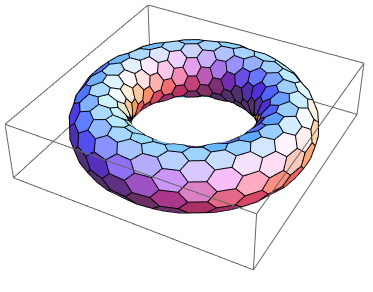
\includegraphics[width=0.75\textwidth]{images/test_image}
%	\caption{Comparing Nuclear Fusion and Fission} ~\\
%	\small The binding energy per nucleon is what differentiates nuclear fusion from fission. Nuclei heavier than Iron fission (e.g.\ Uranium), while light ones -- such as Hydrogen -- fuse. 
%	\label{fig:binding_energy}
%\end{figure}

%\cref{fig:binding_energy}
\deleted{The natural place to start when talking about fusion is the binding-energy per nucleon plot (see Fig. N). As can be seen, the function reaches a maximum value around the element Iron (A=56). What this means at a basic level is: elements lighter than iron can \emph{fuse} into a heavier one (i.e.\ hydrogens into helium), whereas heavier elements can \emph{fission} into lighter ones (e.g.\ uranium into krypton and barium). This is what differentiates fission (uranium-fueled) reactors from fusion (hydrogen-fueled) ones. For fusion reactors, the most common reaction in a first-generation tokamak will be:}

%\begin{equation}
%	{}^2H+ {}^3H \rightarrow {}^4 He + {}^1 n + E_F
%\end{equation}
%\myequations{Fusion Energy -- $E_F$}

%\begin{equation}
%	E_F = 17.6 \ \textnormal{MeV}
%\end{equation}

\deleted{What this reaction describes is two isotopes of hydrogen -- i.e.\ deuterium and tritium -- fusing into a heavier element, helium, while simultaneously ejecting a neutron. The entire energy of the fusion reaction ($E_F$) is then divvied up 80-20 between the neutron and helium, respectively. Quantitatively, the helium (hereafter referred to as an alpha particle) receives 3.5 MeV.}

%\begin{figure}
%	\centering
%	\begin{adjustbox}{width=0.75\textwidth}
%		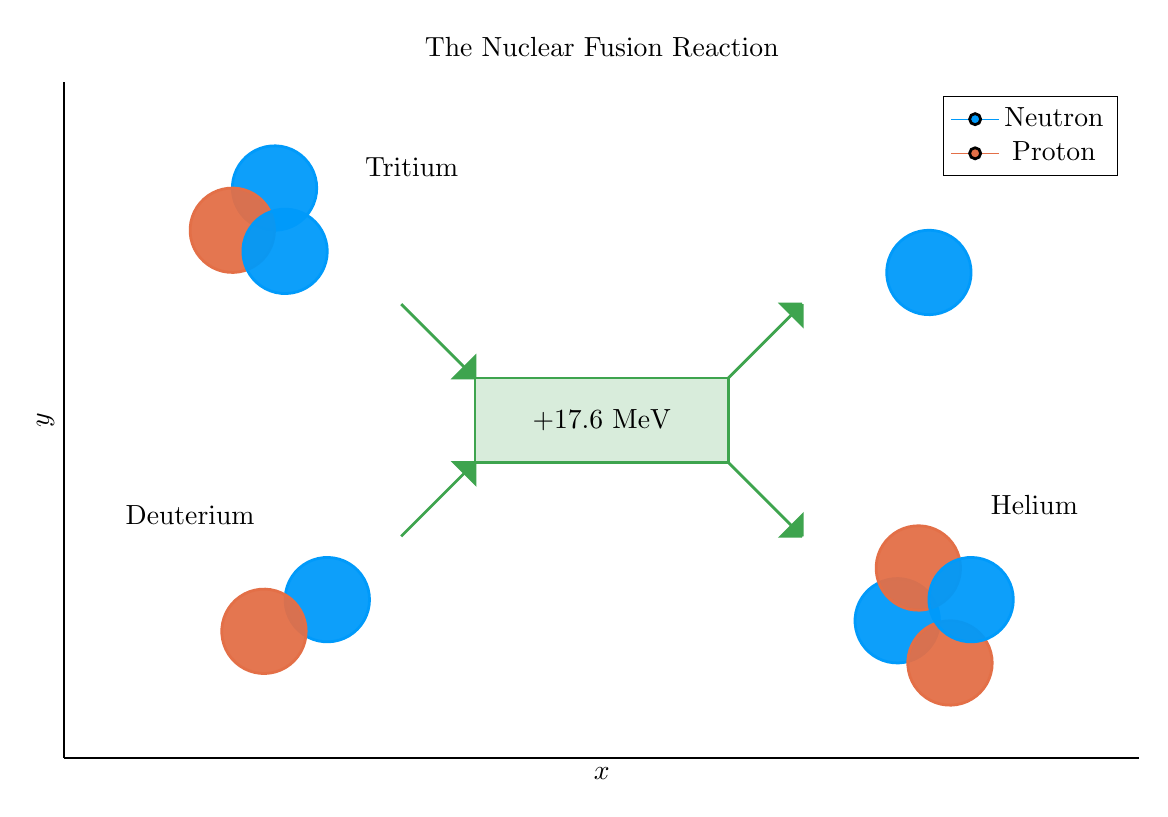
\begin{tikzpicture}[]
\begin{axis}[height = {101.6mm}, axis equal = {true}, ylabel = {$y$}, title = {The Nuclear Fusion Reaction}, xmin = {-12}, xmax = {12}, ymax = {8}, xlabel = {$x$}, {unbounded coords=jump, scaled x ticks = false, xticklabel style={rotate = 0}, xmajorticks=false, xmajorgrids = false, axis lines* = left, scaled y ticks = false, yticklabel style={rotate = 0}, ymajorticks=false, ymajorgrids = false, axis lines* = left,     xshift = 0.0mm,
    yshift = 0.0mm,
    axis background/.style={fill={rgb,1:red,1.00000000;green,1.00000000;blue,1.00000000}}
}, ymin = {-8}, width = {152.4mm}]\addplot+ [color = {rgb,1:red,0.00000000;green,0.60560316;blue,0.97868012},
draw opacity=1.0,
line width=1,
solid,mark = none,
mark size = 2.0,
mark options = {
    color = {rgb,1:red,0.00000000;green,0.00000000;blue,0.00000000}, draw opacity = 1.0,
    fill = {rgb,1:red,0.00000000;green,0.60560316;blue,0.97868012}, fill opacity = 1.0,
    line width = 1,
    rotate = 0,
    solid
},fill = {rgb,1:red,0.00000000;green,0.60560316;blue,0.97868012}, fill opacity=0.95,forget plot]coordinates {
(-6.75, 5.5)
(-6.7582099861767535, 5.627877161684506)
(-6.7827051369609705, 5.7536545839095075)
(-6.823083242653978, 5.875267004879374)
(-6.878681295876611, 5.990717552003938)
(-6.948586378132044, 6.0981105304912155)
(-7.031650649902272, 6.195682550603486)
(-7.126510198141267, 6.2818314824680295)
(-7.231607431689475, 6.355142763005346)
(-7.345216656877606, 6.414412623015813)
(-7.465472413368968, 6.45866785303666)
(-7.590400104966621, 6.48718178341445)
(-7.717948422428345, 6.499486216200688)
(-7.846023025907682, 6.495379112949198)
(-7.972520933956314, 6.4749279121818235)
(-8.095365054421308, 6.438468422049761)
(-8.212538290240834, 6.386599306373)
(-8.32211666012217, 6.320172254596956)
(-8.422300890261317, 6.2402779970753155)
(-8.511445958369134, 6.148228395307789)
(-8.58808810489184, 6.045534901210549)
(-8.650968867902419, 5.933883739117558)
(-8.699055747010668, 5.815108218023621)
(-8.731559156991064, 5.6911586287013725)
(-8.747945392750337, 5.564070219980713)
(-8.747945392750337, 5.435929780019287)
(-8.731559156991064, 5.3088413712986275)
(-8.699055747010668, 5.184891781976379)
(-8.650968867902419, 5.066116260882442)
(-8.58808810489184, 4.954465098789451)
(-8.511445958369135, 4.851771604692212)
(-8.422300890261317, 4.7597220029246845)
(-8.32211666012217, 4.679827745403045)
(-8.212538290240836, 4.613400693627)
(-8.095365054421308, 4.56153157795024)
(-7.972520933956314, 4.5250720878181765)
(-7.846023025907682, 4.504620887050802)
(-7.7179484224283454, 4.500513783799312)
(-7.590400104966621, 4.51281821658555)
(-7.465472413368968, 4.541332146963339)
(-7.345216656877606, 4.585587376984187)
(-7.231607431689476, 4.644857236994653)
(-7.126510198141267, 4.71816851753197)
(-7.031650649902272, 4.804317449396514)
(-6.948586378132044, 4.901889469508784)
(-6.878681295876611, 5.009282447996062)
(-6.823083242653978, 5.124732995120626)
(-6.7827051369609705, 5.2463454160904925)
(-6.7582099861767535, 5.3721228383154935)
(-6.75, 5.5)
};
\addplot+ [color = {rgb,1:red,0.88887350;green,0.43564919;blue,0.27812294},
draw opacity=1.0,
line width=1,
solid,mark = none,
mark size = 2.0,
mark options = {
    color = {rgb,1:red,0.00000000;green,0.00000000;blue,0.00000000}, draw opacity = 1.0,
    fill = {rgb,1:red,0.88887350;green,0.43564919;blue,0.27812294}, fill opacity = 1.0,
    line width = 1,
    rotate = 0,
    solid
},fill = {rgb,1:red,0.88887350;green,0.43564919;blue,0.27812294}, fill opacity=0.95,forget plot]coordinates {
(-7.75, 4.5)
(-7.7582099861767535, 4.627877161684506)
(-7.7827051369609705, 4.7536545839095075)
(-7.823083242653978, 4.875267004879374)
(-7.878681295876611, 4.990717552003938)
(-7.948586378132044, 5.0981105304912155)
(-8.031650649902272, 5.195682550603486)
(-8.126510198141267, 5.2818314824680295)
(-8.231607431689476, 5.355142763005346)
(-8.345216656877605, 5.414412623015813)
(-8.465472413368968, 5.45866785303666)
(-8.590400104966621, 5.48718178341445)
(-8.717948422428345, 5.499486216200688)
(-8.846023025907682, 5.495379112949198)
(-8.972520933956314, 5.4749279121818235)
(-9.095365054421308, 5.438468422049761)
(-9.212538290240834, 5.386599306373)
(-9.32211666012217, 5.320172254596956)
(-9.422300890261317, 5.2402779970753155)
(-9.511445958369134, 5.148228395307789)
(-9.58808810489184, 5.045534901210549)
(-9.650968867902419, 4.933883739117558)
(-9.699055747010668, 4.815108218023621)
(-9.731559156991064, 4.6911586287013725)
(-9.747945392750337, 4.564070219980713)
(-9.747945392750337, 4.435929780019287)
(-9.731559156991064, 4.3088413712986275)
(-9.699055747010668, 4.184891781976379)
(-9.650968867902419, 4.066116260882442)
(-9.58808810489184, 3.9544650987894516)
(-9.511445958369135, 3.8517716046922117)
(-9.422300890261317, 3.7597220029246845)
(-9.32211666012217, 3.6798277454030446)
(-9.212538290240836, 3.613400693627)
(-9.095365054421308, 3.5615315779502397)
(-8.972520933956314, 3.5250720878181765)
(-8.846023025907682, 3.5046208870508018)
(-8.717948422428345, 3.5005137837993123)
(-8.590400104966621, 3.5128182165855497)
(-8.465472413368968, 3.541332146963339)
(-8.345216656877607, 3.5855873769841873)
(-8.231607431689476, 3.6448572369946537)
(-8.126510198141267, 3.71816851753197)
(-8.031650649902272, 3.804317449396514)
(-7.948586378132044, 3.9018894695087836)
(-7.878681295876611, 4.009282447996062)
(-7.823083242653978, 4.124732995120626)
(-7.7827051369609705, 4.2463454160904925)
(-7.7582099861767535, 4.3721228383154935)
(-7.75, 4.5)
};
\addplot+ [color = {rgb,1:red,0.00000000;green,0.60560316;blue,0.97868012},
draw opacity=1.0,
line width=1,
solid,mark = none,
mark size = 2.0,
mark options = {
    color = {rgb,1:red,0.00000000;green,0.00000000;blue,0.00000000}, draw opacity = 1.0,
    fill = {rgb,1:red,0.00000000;green,0.60560316;blue,0.97868012}, fill opacity = 1.0,
    line width = 1,
    rotate = 0,
    solid
},fill = {rgb,1:red,0.00000000;green,0.60560316;blue,0.97868012}, fill opacity=0.95,forget plot]coordinates {
(-6.5, 4.0)
(-6.5082099861767535, 4.127877161684506)
(-6.5327051369609705, 4.2536545839095075)
(-6.573083242653978, 4.375267004879374)
(-6.628681295876611, 4.490717552003938)
(-6.698586378132044, 4.5981105304912155)
(-6.781650649902272, 4.695682550603486)
(-6.876510198141267, 4.7818314824680295)
(-6.981607431689475, 4.855142763005346)
(-7.095216656877606, 4.914412623015813)
(-7.215472413368968, 4.95866785303666)
(-7.340400104966621, 4.98718178341445)
(-7.467948422428345, 4.999486216200688)
(-7.596023025907682, 4.995379112949198)
(-7.722520933956314, 4.9749279121818235)
(-7.845365054421308, 4.938468422049761)
(-7.962538290240835, 4.886599306373)
(-8.07211666012217, 4.820172254596956)
(-8.172300890261317, 4.7402779970753155)
(-8.261445958369134, 4.648228395307789)
(-8.33808810489184, 4.545534901210549)
(-8.400968867902419, 4.433883739117558)
(-8.449055747010668, 4.315108218023621)
(-8.481559156991064, 4.1911586287013725)
(-8.497945392750337, 4.064070219980713)
(-8.497945392750337, 3.935929780019287)
(-8.481559156991064, 3.8088413712986275)
(-8.449055747010668, 3.6848917819763796)
(-8.400968867902419, 3.566116260882442)
(-8.33808810489184, 3.4544650987894516)
(-8.261445958369135, 3.3517716046922117)
(-8.172300890261317, 3.2597220029246845)
(-8.07211666012217, 3.1798277454030446)
(-7.962538290240835, 3.113400693627)
(-7.8453650544213085, 3.0615315779502397)
(-7.722520933956314, 3.0250720878181765)
(-7.596023025907682, 3.0046208870508018)
(-7.4679484224283454, 3.0005137837993123)
(-7.340400104966621, 3.0128182165855497)
(-7.215472413368968, 3.041332146963339)
(-7.095216656877606, 3.0855873769841873)
(-6.981607431689476, 3.1448572369946537)
(-6.876510198141267, 3.21816851753197)
(-6.781650649902272, 3.304317449396514)
(-6.698586378132044, 3.4018894695087836)
(-6.628681295876611, 3.5092824479960623)
(-6.573083242653978, 3.6247329951206253)
(-6.5327051369609705, 3.7463454160904925)
(-6.5082099861767535, 3.8721228383154935)
(-6.5, 3.9999999999999996)
};
\addplot+ [color = {rgb,1:red,0.00000000;green,0.60560316;blue,0.97868012},
draw opacity=1.0,
line width=1,
solid,mark = none,
mark size = 2.0,
mark options = {
    color = {rgb,1:red,0.00000000;green,0.00000000;blue,0.00000000}, draw opacity = 1.0,
    fill = {rgb,1:red,0.00000000;green,0.60560316;blue,0.97868012}, fill opacity = 1.0,
    line width = 1,
    rotate = 0,
    solid
},fill = {rgb,1:red,0.00000000;green,0.60560316;blue,0.97868012}, fill opacity=0.95,forget plot]coordinates {
(-5.5, -4.25)
(-5.5082099861767535, -4.122122838315494)
(-5.5327051369609705, -3.9963454160904925)
(-5.573083242653978, -3.8747329951206257)
(-5.628681295876611, -3.7592824479960623)
(-5.698586378132044, -3.651889469508784)
(-5.781650649902272, -3.5543174493965135)
(-5.876510198141267, -3.46816851753197)
(-5.981607431689475, -3.394857236994654)
(-6.095216656877606, -3.3355873769841873)
(-6.215472413368968, -3.2913321469633394)
(-6.340400104966621, -3.2628182165855497)
(-6.467948422428345, -3.2505137837993123)
(-6.596023025907682, -3.2546208870508018)
(-6.722520933956314, -3.2750720878181765)
(-6.845365054421308, -3.3115315779502397)
(-6.962538290240835, -3.363400693627)
(-7.07211666012217, -3.429827745403044)
(-7.172300890261317, -3.5097220029246845)
(-7.261445958369134, -3.6017716046922117)
(-7.338088104891841, -3.704465098789451)
(-7.400968867902419, -3.816116260882442)
(-7.449055747010669, -3.934891781976379)
(-7.481559156991065, -4.0588413712986275)
(-7.497945392750337, -4.185929780019287)
(-7.497945392750337, -4.314070219980713)
(-7.481559156991065, -4.4411586287013725)
(-7.449055747010669, -4.565108218023621)
(-7.400968867902419, -4.683883739117558)
(-7.338088104891841, -4.795534901210549)
(-7.261445958369134, -4.898228395307788)
(-7.172300890261317, -4.9902779970753155)
(-7.07211666012217, -5.070172254596955)
(-6.962538290240835, -5.136599306373)
(-6.8453650544213085, -5.18846842204976)
(-6.722520933956314, -5.2249279121818235)
(-6.596023025907682, -5.245379112949198)
(-6.4679484224283454, -5.249486216200688)
(-6.340400104966621, -5.23718178341445)
(-6.215472413368968, -5.208667853036661)
(-6.095216656877606, -5.164412623015813)
(-5.981607431689476, -5.105142763005347)
(-5.876510198141267, -5.03183148246803)
(-5.781650649902272, -4.945682550603486)
(-5.698586378132044, -4.848110530491216)
(-5.628681295876611, -4.740717552003938)
(-5.573083242653978, -4.625267004879374)
(-5.5327051369609705, -4.5036545839095075)
(-5.5082099861767535, -4.3778771616845065)
(-5.5, -4.25)
};
\addplot+ [color = {rgb,1:red,0.88887350;green,0.43564919;blue,0.27812294},
draw opacity=1.0,
line width=1,
solid,mark = none,
mark size = 2.0,
mark options = {
    color = {rgb,1:red,0.00000000;green,0.00000000;blue,0.00000000}, draw opacity = 1.0,
    fill = {rgb,1:red,0.88887350;green,0.43564919;blue,0.27812294}, fill opacity = 1.0,
    line width = 1,
    rotate = 0,
    solid
},fill = {rgb,1:red,0.88887350;green,0.43564919;blue,0.27812294}, fill opacity=0.95,forget plot]coordinates {
(-7.0, -5.0)
(-7.0082099861767535, -4.872122838315494)
(-7.0327051369609705, -4.7463454160904925)
(-7.073083242653978, -4.624732995120626)
(-7.128681295876611, -4.509282447996062)
(-7.198586378132044, -4.4018894695087845)
(-7.281650649902272, -4.304317449396514)
(-7.376510198141267, -4.2181685175319705)
(-7.481607431689475, -4.144857236994654)
(-7.595216656877606, -4.085587376984187)
(-7.715472413368968, -4.04133214696334)
(-7.840400104966621, -4.01281821658555)
(-7.967948422428345, -4.000513783799312)
(-8.096023025907682, -4.004620887050802)
(-8.222520933956314, -4.0250720878181765)
(-8.345365054421308, -4.061531577950239)
(-8.462538290240834, -4.113400693627)
(-8.57211666012217, -4.179827745403044)
(-8.672300890261317, -4.2597220029246845)
(-8.761445958369134, -4.351771604692211)
(-8.83808810489184, -4.454465098789451)
(-8.900968867902419, -4.566116260882442)
(-8.949055747010668, -4.684891781976379)
(-8.981559156991064, -4.8088413712986275)
(-8.997945392750337, -4.935929780019287)
(-8.997945392750337, -5.064070219980713)
(-8.981559156991064, -5.1911586287013725)
(-8.949055747010668, -5.315108218023621)
(-8.900968867902419, -5.433883739117558)
(-8.83808810489184, -5.545534901210549)
(-8.761445958369135, -5.648228395307788)
(-8.672300890261317, -5.7402779970753155)
(-8.57211666012217, -5.820172254596955)
(-8.462538290240836, -5.886599306373)
(-8.345365054421308, -5.93846842204976)
(-8.222520933956314, -5.9749279121818235)
(-8.096023025907682, -5.995379112949198)
(-7.9679484224283454, -5.999486216200688)
(-7.840400104966621, -5.98718178341445)
(-7.715472413368968, -5.958667853036661)
(-7.595216656877606, -5.914412623015813)
(-7.481607431689476, -5.855142763005347)
(-7.376510198141267, -5.78183148246803)
(-7.281650649902272, -5.695682550603486)
(-7.198586378132044, -5.598110530491216)
(-7.128681295876611, -5.490717552003938)
(-7.073083242653978, -5.375267004879374)
(-7.0327051369609705, -5.2536545839095075)
(-7.0082099861767535, -5.1278771616845065)
(-7.0, -5.0)
};
\addplot+ [color = {rgb,1:red,0.24222430;green,0.64327509;blue,0.30444865},
draw opacity=1.0,
line width=1,
solid,mark = none,
mark size = 2.0,
mark options = {
    color = {rgb,1:red,0.00000000;green,0.00000000;blue,0.00000000}, draw opacity = 1.0,
    fill = {rgb,1:red,0.24222430;green,0.64327509;blue,0.30444865}, fill opacity = 1.0,
    line width = 1,
    rotate = 0,
    solid
},forget plot]coordinates {
(-4.75, 2.75)
(-3.0, 1.0)
};
\addplot+ [color = {rgb,1:red,0.24222430;green,0.64327509;blue,0.30444865},
draw opacity=1.0,
line width=1,
solid,mark = none,
mark size = 2.0,
mark options = {
    color = {rgb,1:red,0.00000000;green,0.00000000;blue,0.00000000}, draw opacity = 1.0,
    fill = {rgb,1:red,0.24222430;green,0.64327509;blue,0.30444865}, fill opacity = 1.0,
    line width = 1,
    rotate = 0,
    solid
},forget plot]coordinates {
(-4.75, -2.75)
(-3.0, -1.0)
};
\addplot+ [color = {rgb,1:red,0.24222430;green,0.64327509;blue,0.30444865},
draw opacity=1.0,
line width=1,
solid,mark = none,
mark size = 2.0,
mark options = {
    color = {rgb,1:red,0.00000000;green,0.00000000;blue,0.00000000}, draw opacity = 1.0,
    fill = {rgb,1:red,0.24222430;green,0.64327509;blue,0.30444865}, fill opacity = 1.0,
    line width = 1,
    rotate = 0,
    solid
},fill = {rgb,1:red,0.24222430;green,0.64327509;blue,0.30444865}, fill opacity=1.0,forget plot]coordinates {
(-3.0, 1.0)
(-3.5, 1.0)
(-3.0, 1.5)
(-3.0, 1.0)
};
\addplot+ [color = {rgb,1:red,0.24222430;green,0.64327509;blue,0.30444865},
draw opacity=1.0,
line width=1,
solid,mark = none,
mark size = 2.0,
mark options = {
    color = {rgb,1:red,0.00000000;green,0.00000000;blue,0.00000000}, draw opacity = 1.0,
    fill = {rgb,1:red,0.24222430;green,0.64327509;blue,0.30444865}, fill opacity = 1.0,
    line width = 1,
    rotate = 0,
    solid
},fill = {rgb,1:red,0.24222430;green,0.64327509;blue,0.30444865}, fill opacity=1.0,forget plot]coordinates {
(-3.0, -1.0)
(-3.5, -1.0)
(-3.0, -1.5)
(-3.0, -1.0)
};
\addplot+ [color = {rgb,1:red,0.24222430;green,0.64327509;blue,0.30444865},
draw opacity=1.0,
line width=1,
solid,mark = none,
mark size = 2.0,
mark options = {
    color = {rgb,1:red,0.00000000;green,0.00000000;blue,0.00000000}, draw opacity = 1.0,
    fill = {rgb,1:red,0.24222430;green,0.64327509;blue,0.30444865}, fill opacity = 1.0,
    line width = 1,
    rotate = 0,
    solid
},forget plot]coordinates {
(3.0, 1.0)
(4.75, 2.75)
};
\addplot+ [color = {rgb,1:red,0.24222430;green,0.64327509;blue,0.30444865},
draw opacity=1.0,
line width=1,
solid,mark = none,
mark size = 2.0,
mark options = {
    color = {rgb,1:red,0.00000000;green,0.00000000;blue,0.00000000}, draw opacity = 1.0,
    fill = {rgb,1:red,0.24222430;green,0.64327509;blue,0.30444865}, fill opacity = 1.0,
    line width = 1,
    rotate = 0,
    solid
},forget plot]coordinates {
(3.0, -1.0)
(4.75, -2.75)
};
\addplot+ [color = {rgb,1:red,0.24222430;green,0.64327509;blue,0.30444865},
draw opacity=1.0,
line width=1,
solid,mark = none,
mark size = 2.0,
mark options = {
    color = {rgb,1:red,0.00000000;green,0.00000000;blue,0.00000000}, draw opacity = 1.0,
    fill = {rgb,1:red,0.24222430;green,0.64327509;blue,0.30444865}, fill opacity = 1.0,
    line width = 1,
    rotate = 0,
    solid
},fill = {rgb,1:red,0.24222430;green,0.64327509;blue,0.30444865}, fill opacity=1.0,forget plot]coordinates {
(4.75, 2.75)
(4.25, 2.75)
(4.75, 2.25)
(4.75, 2.75)
};
\addplot+ [color = {rgb,1:red,0.24222430;green,0.64327509;blue,0.30444865},
draw opacity=1.0,
line width=1,
solid,mark = none,
mark size = 2.0,
mark options = {
    color = {rgb,1:red,0.00000000;green,0.00000000;blue,0.00000000}, draw opacity = 1.0,
    fill = {rgb,1:red,0.24222430;green,0.64327509;blue,0.30444865}, fill opacity = 1.0,
    line width = 1,
    rotate = 0,
    solid
},fill = {rgb,1:red,0.24222430;green,0.64327509;blue,0.30444865}, fill opacity=1.0,forget plot]coordinates {
(4.75, -2.75)
(4.25, -2.75)
(4.75, -2.25)
(4.75, -2.75)
};
\addplot+ [color = {rgb,1:red,0.24222430;green,0.64327509;blue,0.30444865},
draw opacity=1.0,
line width=1,
solid,mark = none,
mark size = 2.0,
mark options = {
    color = {rgb,1:red,0.00000000;green,0.00000000;blue,0.00000000}, draw opacity = 1.0,
    fill = {rgb,1:red,0.24222430;green,0.64327509;blue,0.30444865}, fill opacity = 1.0,
    line width = 1,
    rotate = 0,
    solid
},fill = {rgb,1:red,0.24222430;green,0.64327509;blue,0.30444865}, fill opacity=0.2,forget plot]coordinates {
(-3, 1)
(3, 1)
(3, -1)
(-3, -1)
(-3, 1)
};
\addplot+ [color = {rgb,1:red,0.00000000;green,0.60560316;blue,0.97868012},
draw opacity=1.0,
line width=1,
solid,mark = none,
mark size = 2.0,
mark options = {
    color = {rgb,1:red,0.00000000;green,0.00000000;blue,0.00000000}, draw opacity = 1.0,
    fill = {rgb,1:red,0.00000000;green,0.60560316;blue,0.97868012}, fill opacity = 1.0,
    line width = 1,
    rotate = 0,
    solid
},fill = {rgb,1:red,0.00000000;green,0.60560316;blue,0.97868012}, fill opacity=0.95,forget plot]coordinates {
(8.75, 3.5)
(8.741790013823246, 3.627877161684506)
(8.71729486303903, 3.7536545839095075)
(8.67691675734602, 3.8752670048793743)
(8.62131870412339, 3.9907175520039377)
(8.551413621867956, 4.0981105304912155)
(8.468349350097728, 4.195682550603486)
(8.373489801858733, 4.2818314824680295)
(8.268392568310524, 4.355142763005346)
(8.154783343122395, 4.414412623015813)
(8.034527586631032, 4.45866785303666)
(7.909599895033379, 4.48718178341445)
(7.782051577571655, 4.499486216200688)
(7.653976974092318, 4.495379112949198)
(7.527479066043686, 4.4749279121818235)
(7.404634945578692, 4.438468422049761)
(7.287461709759165, 4.386599306373)
(7.17788333987783, 4.320172254596956)
(7.077699109738683, 4.2402779970753155)
(6.988554041630866, 4.148228395307789)
(6.911911895108159, 4.045534901210549)
(6.849031132097581, 3.933883739117558)
(6.800944252989331, 3.815108218023621)
(6.768440843008935, 3.6911586287013725)
(6.752054607249663, 3.5640702199807133)
(6.752054607249663, 3.435929780019287)
(6.768440843008935, 3.3088413712986275)
(6.800944252989331, 3.1848917819763796)
(6.849031132097581, 3.066116260882442)
(6.911911895108159, 2.9544650987894516)
(6.988554041630866, 2.8517716046922117)
(7.077699109738683, 2.7597220029246845)
(7.17788333987783, 2.6798277454030446)
(7.287461709759165, 2.613400693627)
(7.4046349455786915, 2.5615315779502397)
(7.527479066043686, 2.5250720878181765)
(7.653976974092318, 2.5046208870508018)
(7.7820515775716546, 2.5005137837993123)
(7.909599895033379, 2.5128182165855497)
(8.034527586631032, 2.541332146963339)
(8.154783343122393, 2.5855873769841873)
(8.268392568310524, 2.6448572369946537)
(8.373489801858733, 2.71816851753197)
(8.468349350097728, 2.804317449396514)
(8.551413621867956, 2.9018894695087836)
(8.62131870412339, 3.0092824479960623)
(8.67691675734602, 3.1247329951206253)
(8.71729486303903, 3.2463454160904925)
(8.741790013823246, 3.3721228383154935)
(8.75, 3.4999999999999996)
};
\addplot+ [color = {rgb,1:red,0.00000000;green,0.60560316;blue,0.97868012},
draw opacity=1.0,
line width=1,
solid,mark = none,
mark size = 2.0,
mark options = {
    color = {rgb,1:red,0.00000000;green,0.00000000;blue,0.00000000}, draw opacity = 1.0,
    fill = {rgb,1:red,0.00000000;green,0.60560316;blue,0.97868012}, fill opacity = 1.0,
    line width = 1,
    rotate = 0,
    solid
},fill = {rgb,1:red,0.00000000;green,0.60560316;blue,0.97868012}, fill opacity=0.95,forget plot]coordinates {
(8.0, -4.75)
(7.9917900138232465, -4.622122838315494)
(7.9672948630390295, -4.4963454160904925)
(7.926916757346022, -4.374732995120626)
(7.871318704123389, -4.259282447996062)
(7.801413621867956, -4.1518894695087845)
(7.718349350097728, -4.054317449396514)
(7.623489801858733, -3.96816851753197)
(7.518392568310525, -3.894857236994654)
(7.404783343122394, -3.8355873769841873)
(7.284527586631032, -3.7913321469633394)
(7.159599895033379, -3.7628182165855497)
(7.032051577571655, -3.7505137837993123)
(6.903976974092318, -3.7546208870508018)
(6.777479066043686, -3.7750720878181765)
(6.654634945578692, -3.8115315779502397)
(6.537461709759165, -3.863400693627)
(6.42788333987783, -3.929827745403044)
(6.327699109738683, -4.0097220029246845)
(6.238554041630866, -4.101771604692211)
(6.161911895108159, -4.204465098789451)
(6.099031132097581, -4.316116260882442)
(6.050944252989331, -4.434891781976379)
(6.018440843008935, -4.5588413712986275)
(6.002054607249663, -4.685929780019287)
(6.002054607249663, -4.814070219980713)
(6.018440843008935, -4.9411586287013725)
(6.050944252989331, -5.065108218023621)
(6.099031132097581, -5.183883739117558)
(6.161911895108159, -5.295534901210549)
(6.238554041630866, -5.398228395307788)
(6.327699109738683, -5.4902779970753155)
(6.42788333987783, -5.570172254596955)
(6.537461709759165, -5.636599306373)
(6.6546349455786915, -5.68846842204976)
(6.777479066043686, -5.7249279121818235)
(6.903976974092318, -5.745379112949198)
(7.0320515775716546, -5.749486216200688)
(7.159599895033379, -5.73718178341445)
(7.284527586631032, -5.708667853036661)
(7.404783343122394, -5.664412623015813)
(7.518392568310524, -5.605142763005347)
(7.623489801858733, -5.53183148246803)
(7.718349350097728, -5.445682550603486)
(7.801413621867956, -5.348110530491216)
(7.871318704123389, -5.240717552003938)
(7.926916757346022, -5.125267004879374)
(7.9672948630390295, -5.0036545839095075)
(7.9917900138232465, -4.8778771616845065)
(8.0, -4.75)
};
\addplot+ [color = {rgb,1:red,0.88887350;green,0.43564919;blue,0.27812294},
draw opacity=1.0,
line width=1,
solid,mark = none,
mark size = 2.0,
mark options = {
    color = {rgb,1:red,0.00000000;green,0.00000000;blue,0.00000000}, draw opacity = 1.0,
    fill = {rgb,1:red,0.88887350;green,0.43564919;blue,0.27812294}, fill opacity = 1.0,
    line width = 1,
    rotate = 0,
    solid
},fill = {rgb,1:red,0.88887350;green,0.43564919;blue,0.27812294}, fill opacity=0.95,forget plot]coordinates {
(9.25, -5.75)
(9.241790013823246, -5.622122838315494)
(9.21729486303903, -5.4963454160904925)
(9.17691675734602, -5.374732995120626)
(9.12131870412339, -5.259282447996062)
(9.051413621867956, -5.1518894695087845)
(8.968349350097728, -5.054317449396514)
(8.873489801858733, -4.9681685175319705)
(8.768392568310524, -4.894857236994654)
(8.654783343122395, -4.835587376984187)
(8.534527586631032, -4.79133214696334)
(8.409599895033379, -4.76281821658555)
(8.282051577571655, -4.750513783799312)
(8.153976974092318, -4.754620887050802)
(8.027479066043686, -4.7750720878181765)
(7.904634945578692, -4.811531577950239)
(7.787461709759165, -4.863400693627)
(7.67788333987783, -4.929827745403044)
(7.577699109738683, -5.0097220029246845)
(7.488554041630866, -5.101771604692211)
(7.411911895108159, -5.204465098789451)
(7.349031132097581, -5.316116260882442)
(7.300944252989331, -5.434891781976379)
(7.268440843008935, -5.5588413712986275)
(7.252054607249663, -5.685929780019287)
(7.252054607249663, -5.814070219980713)
(7.268440843008935, -5.9411586287013725)
(7.300944252989331, -6.065108218023621)
(7.349031132097581, -6.183883739117558)
(7.411911895108159, -6.295534901210549)
(7.488554041630866, -6.398228395307788)
(7.577699109738683, -6.4902779970753155)
(7.67788333987783, -6.570172254596955)
(7.787461709759165, -6.636599306373)
(7.9046349455786915, -6.68846842204976)
(8.027479066043686, -6.7249279121818235)
(8.153976974092318, -6.745379112949198)
(8.282051577571655, -6.749486216200688)
(8.409599895033379, -6.73718178341445)
(8.534527586631032, -6.708667853036661)
(8.654783343122393, -6.664412623015813)
(8.768392568310524, -6.605142763005347)
(8.873489801858733, -6.53183148246803)
(8.968349350097728, -6.445682550603486)
(9.051413621867956, -6.348110530491216)
(9.12131870412339, -6.240717552003938)
(9.17691675734602, -6.125267004879374)
(9.21729486303903, -6.0036545839095075)
(9.241790013823246, -5.8778771616845065)
(9.25, -5.75)
};
\addplot+ [color = {rgb,1:red,0.88887350;green,0.43564919;blue,0.27812294},
draw opacity=1.0,
line width=1,
solid,mark = none,
mark size = 2.0,
mark options = {
    color = {rgb,1:red,0.00000000;green,0.00000000;blue,0.00000000}, draw opacity = 1.0,
    fill = {rgb,1:red,0.88887350;green,0.43564919;blue,0.27812294}, fill opacity = 1.0,
    line width = 1,
    rotate = 0,
    solid
},fill = {rgb,1:red,0.88887350;green,0.43564919;blue,0.27812294}, fill opacity=0.95,forget plot]coordinates {
(8.5, -3.5)
(8.491790013823246, -3.372122838315494)
(8.46729486303903, -3.2463454160904925)
(8.42691675734602, -3.1247329951206257)
(8.37131870412339, -3.0092824479960623)
(8.301413621867956, -2.901889469508784)
(8.218349350097728, -2.8043174493965135)
(8.123489801858733, -2.71816851753197)
(8.018392568310524, -2.644857236994654)
(7.904783343122394, -2.5855873769841873)
(7.784527586631032, -2.5413321469633394)
(7.659599895033379, -2.5128182165855497)
(7.532051577571655, -2.5005137837993123)
(7.403976974092318, -2.5046208870508018)
(7.277479066043686, -2.5250720878181765)
(7.154634945578692, -2.5615315779502397)
(7.037461709759165, -2.613400693627)
(6.92788333987783, -2.679827745403044)
(6.827699109738683, -2.7597220029246845)
(6.738554041630866, -2.8517716046922117)
(6.661911895108159, -2.954465098789451)
(6.599031132097581, -3.066116260882442)
(6.550944252989331, -3.184891781976379)
(6.518440843008935, -3.3088413712986275)
(6.502054607249663, -3.4359297800192867)
(6.502054607249663, -3.564070219980713)
(6.518440843008935, -3.6911586287013725)
(6.550944252989331, -3.8151082180236204)
(6.599031132097581, -3.933883739117558)
(6.661911895108159, -4.045534901210549)
(6.738554041630866, -4.148228395307788)
(6.827699109738683, -4.2402779970753155)
(6.92788333987783, -4.320172254596955)
(7.037461709759165, -4.386599306373)
(7.1546349455786915, -4.43846842204976)
(7.277479066043686, -4.4749279121818235)
(7.403976974092318, -4.495379112949198)
(7.5320515775716546, -4.499486216200688)
(7.659599895033379, -4.48718178341445)
(7.784527586631032, -4.458667853036661)
(7.904783343122394, -4.414412623015813)
(8.018392568310524, -4.355142763005347)
(8.123489801858733, -4.28183148246803)
(8.218349350097728, -4.195682550603486)
(8.301413621867956, -4.098110530491216)
(8.37131870412339, -3.9907175520039377)
(8.42691675734602, -3.8752670048793747)
(8.46729486303903, -3.7536545839095075)
(8.491790013823246, -3.6278771616845065)
(8.5, -3.5000000000000004)
};
\addplot+ [color = {rgb,1:red,0.00000000;green,0.60560316;blue,0.97868012},
draw opacity=1.0,
line width=1,
solid,mark = none,
mark size = 2.0,
mark options = {
    color = {rgb,1:red,0.00000000;green,0.00000000;blue,0.00000000}, draw opacity = 1.0,
    fill = {rgb,1:red,0.00000000;green,0.60560316;blue,0.97868012}, fill opacity = 1.0,
    line width = 1,
    rotate = 0,
    solid
},fill = {rgb,1:red,0.00000000;green,0.60560316;blue,0.97868012}, fill opacity=0.95,forget plot]coordinates {
(9.75, -4.25)
(9.741790013823246, -4.122122838315494)
(9.71729486303903, -3.9963454160904925)
(9.67691675734602, -3.8747329951206257)
(9.62131870412339, -3.7592824479960623)
(9.551413621867956, -3.651889469508784)
(9.468349350097728, -3.5543174493965135)
(9.373489801858733, -3.46816851753197)
(9.268392568310524, -3.394857236994654)
(9.154783343122395, -3.3355873769841873)
(9.034527586631032, -3.2913321469633394)
(8.909599895033379, -3.2628182165855497)
(8.782051577571655, -3.2505137837993123)
(8.653976974092318, -3.2546208870508018)
(8.527479066043686, -3.2750720878181765)
(8.404634945578692, -3.3115315779502397)
(8.287461709759166, -3.363400693627)
(8.17788333987783, -3.429827745403044)
(8.077699109738683, -3.5097220029246845)
(7.988554041630866, -3.6017716046922117)
(7.911911895108159, -3.704465098789451)
(7.849031132097581, -3.816116260882442)
(7.800944252989331, -3.934891781976379)
(7.768440843008935, -4.0588413712986275)
(7.752054607249663, -4.185929780019287)
(7.752054607249663, -4.314070219980713)
(7.768440843008935, -4.4411586287013725)
(7.800944252989331, -4.565108218023621)
(7.849031132097581, -4.683883739117558)
(7.911911895108159, -4.795534901210549)
(7.988554041630866, -4.898228395307788)
(8.077699109738683, -4.9902779970753155)
(8.17788333987783, -5.070172254596955)
(8.287461709759164, -5.136599306373)
(8.404634945578692, -5.18846842204976)
(8.527479066043686, -5.2249279121818235)
(8.653976974092318, -5.245379112949198)
(8.782051577571655, -5.249486216200688)
(8.909599895033379, -5.23718178341445)
(9.034527586631032, -5.208667853036661)
(9.154783343122393, -5.164412623015813)
(9.268392568310524, -5.105142763005347)
(9.373489801858733, -5.03183148246803)
(9.468349350097728, -4.945682550603486)
(9.551413621867956, -4.848110530491216)
(9.62131870412339, -4.740717552003938)
(9.67691675734602, -4.625267004879374)
(9.71729486303903, -4.5036545839095075)
(9.741790013823246, -4.3778771616845065)
(9.75, -4.25)
};
\addplot+[draw=none, color = {rgb,1:red,0.00000000;green,0.60560316;blue,0.97868012},
draw opacity=1.0,
line width=0,
solid,mark = *,
mark size = 2.0,
mark options = {
    color = {rgb,1:red,0.00000000;green,0.00000000;blue,0.00000000}, draw opacity = 1.0,
    fill = {rgb,1:red,0.00000000;green,0.60560316;blue,0.97868012}, fill opacity = 1.0,
    line width = 1,
    rotate = 0,
    solid
}] coordinates {
(100, 100)
};
\addlegendentry{Neutron}
\addplot+[draw=none, color = {rgb,1:red,0.88887350;green,0.43564919;blue,0.27812294},
draw opacity=1.0,
line width=0,
solid,mark = *,
mark size = 2.0,
mark options = {
    color = {rgb,1:red,0.00000000;green,0.00000000;blue,0.00000000}, draw opacity = 1.0,
    fill = {rgb,1:red,0.88887350;green,0.43564919;blue,0.27812294}, fill opacity = 1.0,
    line width = 1,
    rotate = 0,
    solid
}] coordinates {
(100, 100)
};
\addlegendentry{Proton}
\node at (axis cs:-4.5, 6) [,
color={rgb,1:red,0.00000000;green,0.00000000;blue,0.00000000}, draw opacity=1.0,
rotate=0.0
] {Tritium};
\node at (axis cs:-9.75, -2.25) [,
color={rgb,1:red,0.00000000;green,0.00000000;blue,0.00000000}, draw opacity=1.0,
rotate=0.0
] {Deuterium};
\node at (axis cs:0, 0) [,
color={rgb,1:red,0.00000000;green,0.00000000;blue,0.00000000}, draw opacity=1.0,
rotate=0.0
] {+17.6 MeV};
\node at (axis cs:10.25, -2) [,
color={rgb,1:red,0.00000000;green,0.00000000;blue,0.00000000}, draw opacity=1.0,
rotate=0.0
] {Helium};
\end{axis}

\end{tikzpicture}

%	\end{adjustbox}
%%	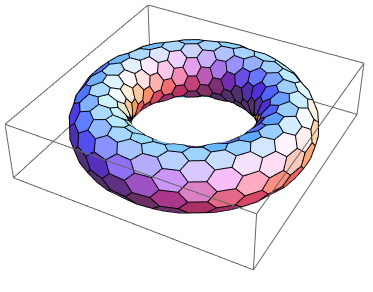
\includegraphics[width=0.75\textwidth]{images/test_image}
%	\caption{The D-T Fusion Reaction} ~\\
%	\small In a first generation tokamak reactor, the main source of energy will come from two hydrogen isotopes fusing into a helium particle -- and ejecting a 14.1 MeV neutron.
%\end{figure}

\deleted{The final point to make before returning to the fusion power derivation is the main difference between the two fusion products: helium (i.e.\ the alpha particle) and the neutron. First, neutrons lack a charge -- they are neutral. This means they cannot be confined with magnetic fields. As such, they simply move in straight lines until they collide with other particles. As the structure of a tokamak is mainly metal, the neutron is much more likely to collide there than the gaseous plasma, which is orders of magnitude less dense. Conversely, alpha particles are charged -- when stripped of their electrons -- and can therefore be kept within the plasma using magnets. What this means practically is that of the 17.6 MeV that comes from every fusion reaction, only 3.5 MeV remains inside the plasma (within the helium particle species).}
 
 \added{The next segue on our journey to solving for the steady current is deriving the fusion power ($P_F$), which appears in current drive. A comprehensive introduction to this is given in \cref{chapter:power}.} \replaced{Summarized, though, a formula for}{Returning to the problem at hand, the} fusion power from a D-T reaction -- in megawatts -- is given by \replaced{the following volume integral: \cite{fusionpower} }{ Jeff Freidberg's textbook through the following volume integral: }
 \begin{equation}
 	\label{eq:pf_int}
 	P_F = \int E_F \, n_D \, n_T \, \langle \sigma v \rangle \, d \vec{\bold{r}}
 \end{equation}
\begin{equation}
	E_F = 17.6 \ \textnormal{MeV}
\end{equation}
\added{The $E_F$ quantity is the energy created from a deuterium-tritium fusion reaction.} The $n_D$ and $n_T$ in this equation \added{then} represent the density of the deuterium and tritium ions, respectively. Assuming a 50-50 mix of the two, they can be related to the electron density -- i.e.\ the one used in this model -- through the dilution factor \added{($f_D$). This dilution factor represents the decrease in available fuel from part of the plasma actually being composed of non-hydrogen gasses}:
 \begin{equation}
 	n_D = n_T = f_D \cdot \left( \frac{n}{2} \right)
 \end{equation}
 \myequations{Dilution Factor -- $f_{D}$}
 The fusion reactivity, $\langle \sigma v \rangle$, is then a nonlinear function of the temperature, T, which the model approximates using the Bosch-Hale tabulation (described in the appendix). As this tabulated value appears inside an integral, it seems important to point out that the temperature is now the most difficult \replaced{dynamic}{floating} variable to handle -- over $R_0$, $B_0$, $\overline n$, and $I_P$. This will come into play when the model is formalized next chapter.
 
 The next step in the derivation of fusion power is transforming the three-dimensional volume integral (see Eq. \ref{eq:pf_int}) into a zero-dimension averaged value. First, the volume analogue of the previously given surface-area integral is:
 \begin{equation}
  	\label{eq:qv}
 	Q_V = 4 \pi^2 R_0 a^2 \kappa g \int_0^1 Q(\rho) \rho \, d\rho
 \end{equation}
 \myequations{Volume Integral -- $Q_V$}
 Where again, Q is an arbitrary function of $\rho$ and g is a geometric factor approximately equal to one. The fusion power can now be rewritten as:
 \begin{equation}
 	P_F = \pi^2 E_F f_D^2 R_0 a^2 \kappa g \int_0^1 n^2 \langle \sigma v \rangle \rho \, d\rho
 \end{equation}
In standardized units, this becomes:
\begin{equation}
	\label{eq:pf}
	\tcboxmath{
	P_F = K_F \cdot \overline{n}^2 \cdot R_0^3  \cdot (\sigma v)
	}
\end{equation}
\myequations{Fusion Power -- $P_F$}
\begin{equation}
  K_F = 278.3 \cdot f_D^2 \cdot ( \epsilon^2 \kappa g )
\end{equation}
Where the standardized fusion reactivity is now,
\begin{equation}
   (\sigma v) = 10^{21} \, (1+\nu_n)^2 \int\limits_0^1 ( 1 - \rho^2 ) ^ { \, 2 \nu_n} \langle \sigma v \rangle \, \rho \, d\rho
\end{equation}
\deleted{As mentioned before, this fusion power is divvied up 80-20 between the neutron and alpha particle. These relations will be used shortly. For now, they can be described mathematically as:}
%\begin{equation}
%	P_\alpha = 0.2 \cdot P_F
%\end{equation}
%\myequations{Alpha Power -- $P_\alpha$}
%\begin{equation}
%	P_n = 0.8 \cdot P_F
%\end{equation}
%\myequations{Neutron Power -- $P_n$}
At this point, the current drive needed for steady-state can now be defined.

\subsection{Using Current Drive}

As may have been lost along the way, \replaced{this chapter's}{the current} mission is to define a formula for steady current -- from the current balance equation for steady-state tokamaks:
\begin{equation}
		\tag{\ref{eq:ibal}}
		I_P = I_{BS} + I_{CD}
\end{equation}
In standardized units, the equation for current drive is often given in the literature as: \cite{itercd}
\begin{equation}
	I_{CD} = \eta_{CD} \cdot \left( \frac{P_H}{\overline n R_0} \right)
\end{equation}
Here, $\eta_{CD}$ is the current drive efficiency with units $ \left(
\frac{ \textnormal{MA} }{ \textnormal{MW-m}^2 } \right) $ and $P_H$ is the heating power in megawatts driven by LHCD (and absorbed by the plasma).

Let it be known, though, that driving current in a plasma is hard! In fact, pulsed reactor designers (i.e.\ European fusion researchers) think it is so difficult, they may choose to forego it completely -- focusing only on inductive sources that necessitate reactor fatigue and downtime. 

A common current drive efficiency ($\eta_{CD}$) seen in many designs is $0.3 \pm 0.1 $ in the standard units. It is however inherently a function of all the plasma parameters -- with subtlety put off until the discussion of self-consistency. For now it assumed to have some constant/\replaced{static}{fixed} value.

The remaining step in deriving an equation for driven current ($I_{CD}$) is a formula for the heating power ($P_H$). The way fusion systems models -- like this one -- handle the heating power is through the physics gain factor, Q. Sometimes referred to as big Q, this value represents how many times over the heating power ($P_H$) is amplified as it is transformed into fusion power ($P_F$):
\begin{equation}
	P_H = \frac{P_F}{Q}
\end{equation}
Now, utilizing the previously defined Greenwald density and fusion power:
 \begin{equation}
 	\tag{\ref{eq:greenwald}}
 	\overline n = K_n \cdot \left( \frac{I_P}{R_0^2} \right)
 \end{equation}
 \begin{equation}
	\tag{\ref{eq:pf}}
	P_F = K_F \cdot \overline{n}^2 \cdot R_0^3  \cdot (\sigma v)
\end{equation}
The current from LHCD can be written as:
\begin{equation}
	\label{eq:icd}
	\tcboxmath{
	I_{CD} = K_{CD} \cdot I_P \cdot ( \sigma v )
	}
\end{equation}
\myequations{Current Drive -- $I_{CD}$}
\begin{equation}
	K_{CD} = \left( K_F K_n \right) \cdot \frac{\eta_{CD}}{Q}
\end{equation}
As $\eta_{CD}$ and Q appear within a \replaced{static}{fixed} coefficient, it is implied that both remain constant throughout a solve. This subtlety is lifted when handling $\eta_{CD}$ self-consistently, which will be discussed shortly. However, even in that context, it proves beneficial to still think of $\eta_{CD}$ as a sequence of \replaced{static}{fixed} variables -- set by the model rather than the user.

\subsection{Completing the Steady Current}

\replaced{The}{As hinted along the way, the} goal of this \replaced{chapter}{section} has been to derive a simple formula for steady current ($I_P$). The problem started with current balance in a steady-state reactor:
\begin{equation}
	\tag{\ref{eq:ibal}}
	I_P = I_{BS} + I_{CD}
\end{equation}
Two equations were then found for the bootstrap ($I_{BS}$) and driven ($I_{CD}$) current:
\begin{equation}
	\tag{\ref{eq:ibs}}
	I_{BS} = K_{BS} \cdot \overline T
\end{equation}
\begin{equation}
	\tag{\ref{eq:icd}}
	I_{CD} = K_{CD} \cdot I_P \cdot ( \sigma v )
\end{equation}
Combining these three equations and solving for the total plasma current ($I_P$) -- in mega-amps -- yields:
\begin{equation}
	\label{eq:steady}
	\tcbhighmath{
	I_P = \frac{ K_{BS} \, \overline T }{ 1 - K_{CD} ( \sigma v ) }
	}
\end{equation}
\myequations{Steady Current -- $I_P$}
This is the answer we have been seeking!

As mentioned before, this simple formula appears to only depend on temperature!\footnote{ This dependence only on temperature refers to dynamic variables. The plasma current can still be highly volatile to many of the static variables, such as: $\epsilon$, $\kappa$, $N_G$, $f_D$, $\nu_n$, $l_i$, etc. } Apparently, the plasma should have the same current at some temperature (i.e.\ $\overline T$ = 15 keV), regardless of the size of the machine or the strength of its magnets. This has the important corollary that each temperature maps to only one current value. \added{Further, each temperature would then map to a single magnet strength, capital cost, etc.\ (as shown next chapter).}

As has become a mantra, though, the subtlety of this behavior lies in the self-consistency of the current-drive efficiency -- $\eta_{CD}$.

\section{Handling Current Drive Self-Consistently}

Although a thorough description of the wave theory behind lower-hybrid current drive (LHCD) is well outside the scope of this text, it does motivate the solving of a tokamak's major radius ($R_0$) and field strength ($B_0$). It also shows how what was once a simple problem has now transformed into a rather complex one -- a common occurrence with plasmas.

The logic behind finding a self-consistent current-drive efficiency is starting at some plausible value (i.e.\ $\eta_{CD} = 0.3$), solving for the steady current -- i.e.\ $I_P = f(\overline T)$ -- and then somehow iteratively creeping towards a value deemed self-consistent. What this means is that in addition to the solver described in the last section, there needs to be a black-box function that solutions are \replaced{sent}{piped} through to get better guesses at $\eta_{CD}$. The black-box function we use is a variation of the Ehst-Karney model. \cite{ehstkarney}

As mentioned, a self-consistent $\eta_{CD}$ is found once a trip through the Ehst-Karney black-box results in the same $\eta_{CD}$ as was \replaced{sent}{piped} in -- to some tolerable level of error. This consistency incorporates an explicit dependence on the tokamak configuration. Mathematically,
\begin{equation}
	\tilde \eta_{CD} = f( R_0, B_0, \overline n, \overline T, I_P )
\end{equation}
\myequations{Current Drive Efficiency -- $\eta_{CD}$}
As such, to recalculate it after every solution of the steady current requires a value for both $B_0$ and $R_0$ -- the targets of this model's primary and \replaced{limiting}{secondary} constraints. These will be the highlight of the next chapter.

%\end{document}

%\documentclass[11pt]{book}
%
%\setlength{\parindent}{0pt}
%\setlength{\parskip}{8pt}
%
%\usepackage{amsmath}
%\usepackage{amssymb}
%\usepackage{hyperref}
%
%\renewcommand*{\thefootnote}{\fnsymbol{footnote}}
%
%\setcounter{chapter}{2}
%
%\begin{document}
%
%\section*{A Levelized Comparison of \\ Pulsed and Steady-State Tokamaks}
%
%\let\cleardoublepage\relax \tableofcontents \newpage

\chapter{Formalizing the Systems Model}

\label{chapter:model}

The goal of this chapter is to take a step back from the steady current derivation and see the larger picture behind reactor design. As such, a more in-depth description of \replaced{static}{fixed} and \replaced{dynamic}{floating} variables is given. This discussion of \replaced{dynamic}{floating} variables will then lend itself to a description of the framework underpinning the fusion systems model. As such, we will now need formulas for the radius and magnet strength of the tokamak. Moving forward, the current will \deleted{then} remain a connecting piece as we \replaced{redirect focus}{switch gears} to pulsed tokamaks and compare \replaced{the underlying solvers of the two schemes.}{the two schemes' underlying solvers.}

\added{The end result of this analysis will then be equations that allow the density ($\overline n$), current ($I_P$), major radius ($R_0$), and magnet strength ($B_0$) to be written as functions of the temperature ($\overline T$) and  static variables (e.g.\ $\nu_n$, $N_G$, $f_D$). These formulas are the product of applying constraints required for all tokamak reactors with several other limiting constraints. The constraints relevant to all tokamak reactors are: the Greenwald limit, current balance, and power balance. Limit constraints then include: the Troyon beta limit, the kink safety factor, the wall loading limit, the maximum power constraint, and the heat loading limit.}

\added{Actual methodologies for solving for the five dynamic variables simultaneously -- i.e.\ $\overline T$, $\overline n$, $I_P$, $R_0$, $B_0$ -- are put off until \cref{chapter:complete}.}

\section{Explaining \replaced{Static}{Fixed} Variables} 

In this model, \replaced{static}{fixed} variables are ones that remain constant while solving for a reactor. These include geometric scalings (i.e.\ $\epsilon$, $\delta$, $\kappa$), profile parameters (i.e.\ $\nu_n$, $\nu_T$, $l_i$), and a \replaced{couple dozen}{slew} of physics constants related to pulsed and steady-state design (e.g.\ Q, $N_G$, $f_D$). For a complete list of \replaced{static}{fixed} variables, consult \replaced{\cref{chapter:var_table}}{the appendix}. The point to make now is that this model treats \replaced{static}{fixed} variables as \replaced{immutable}{second-class} objects. As such they often reside in \replaced{static}{fixed} coefficients -- $K_\square$ -- which are treated as constants.

\section{Connecting \replaced{Dynamic}{Floating} Variables}

\replaced{Dynamic}{Floating} variables -- $\overline T$, $\overline n$, $I_P$, $R_0$, $B_0$ -- are the first-class variables of this fusion systems model. They represent the fundamental properties of a plasma and tokamak (which constitute a fusion reactor). As such, they will be reintroduced one at a time, explaining how they fit into the model -- and which \replaced{equations are}{equation is} capable of representing \replaced{them}{it}.

\begin{table}[h!]
\centering	
\caption{Dynamic Variables}
\begin{tabular}{ c|c|c } 

\textbf{Symbol} & \textbf{Name} & \textbf{Units} \\
\hline
$I_P$ & Plasma Current & MA \\ 
$\overline{T}$ & Plasma Temperature & keV \\ 
$\overline{n}$ & Electron Density & $10^{20} \, \textnormal{m}^{-3}$ \\ 
$R_0$ &  Major Radius & m \\ 
$B_0$ &  Magnetic Field & T
\end{tabular}
\label{table:dynamic}
\end{table}

Bluntly, this fusion systems model is a simple algebra problem: solve five equations with five unknowns (i.e.\ $\overline T$, $\overline n$, $I_P$, $R_0$, $B_0$). Although this naive approach would work, we can do a little better by \replaced{collapsing}{wrangling} these five equations down to just one. This was already done while deriving the steady current. It just happened that the current was not directly dependent on the tokamak size ($R_0$) or magnet strength ($B_0$). 

This will prove more challenging for the generalized current needed for pulsed operation. Even so, this equation will still be \replaced{reduced}{boiled down} to one equation with a single unknown -- $I_P$. A solution to which can be solved much faster than the naive 5 equation approach. This is one reason the model is so fast. 

\subsubsection{The Plasma Temperature -- $\overline T$}

The plasma temperature, measured in keV (kilo-electron-volts), is one of the most \replaced{nonlinear}{finicky} variables in the fusion systems \replaced{framework}{model}. It first proved troublesome when it was shown that a pedestal profile -- not a parabolic one used here -- would be needed for an accurate calculation of bootstrap current. The \replaced{black-box}{unusual} tabulation for reactivity -- ($\sigma v$) -- which appeared in fusion power only further exposed this nonlinearity.

Acknowledging that temperature is the most difficult to handle parameter prompts its use as the scanned variable. What this means practically is scanning temperatures \replaced{is the most straightforward method to produce}{produces} curves of reactors. By example, a scan may be run over the average temperatures ($\overline T$): 10, 15, 20, 25, and 30 keV -- \added{where} each \replaced{corresponds}{corresponding} to its own reactor \added{with its own field strength ($B_0$), plasma current ($I_P$), etc}. In equation form, this becomes:
\begin{equation}
	\label{eq:tbar}
	\overline T = const.
\end{equation}
\myequations{Scanned Temperature -- $\overline T$}
\replaced{The constant value, here,}{Where the constant} happens to be 10 \added{keV} in one run, 15 \added{keV} for the next, and 30 \added{keV} in the fifth.

\subsubsection{The Plasma Density -- $\overline n$}

\replaced{The Greenwald density limit is a constraint with a simple form that applies to all tokamak reactors.}{The cornerstone of this fusion systems model has always been the application of the Greenwald density limit from square one.} It is for this reason -- as well as being a good approximation -- that a parabolic profile was rationalized over a pedestal (H-Mode) one. Repeated, the Greenwald density limit is:
\begin{equation}
	\tag{\ref{eq:greenwald}}
	\overline n = K_n \cdot \frac{I_P}{R_0^2}
\end{equation}
This is an exceptionally simple relationship and why it guided the model. Unlike the next three variables, it is actually used in their derivations. \deleted{Therefore, any reactor found through this model is considered a \emph{Greenwaldian Reactor} -- one held at the Greenwald density limit.}

\subsubsection{The Plasma Current -- $I_P$}

The plasma current is what separates steady-state from pulsed operation. From before, the steady current was found to be:
\begin{equation}
	\tag{\ref{eq:steady}}
	I_P = \frac{K_{BS} \overline T}{1 - K_{CD} ( \sigma v ) }
\end{equation}
This was derived by setting the total current equal to the two sources of current: bootstrap and current drive. Or in fractional form,
\begin{equation}
	I_P = I_{BS} + I_{CD} \ \ \rightarrow \, \ \ 1 = f_{BS} + f_{CD}
\end{equation}
This says that the current fractions of bootstrap and current drive must sum to one. As shown next chapter, inductive sources can be included into this current balance:
\begin{equation}
	\label{eq:ifbal}
	1 = f_{BS} + f_{CD} + f_{ID}
\end{equation}
\begin{figure}
	\centering
	\begin{adjustbox}{width=0.75\textwidth}
		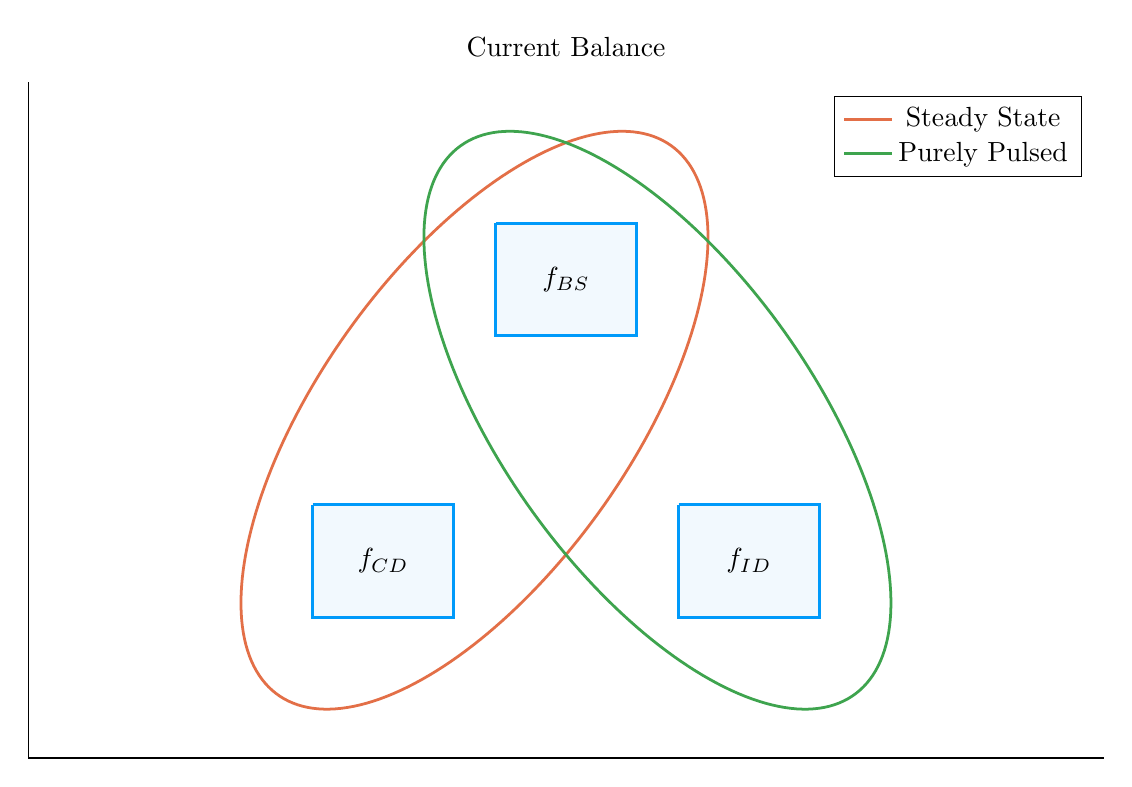
\begin{tikzpicture}[]
\begin{axis}[height = {101.6mm}, axis equal = {true}, ylabel = {}, title = {Current Balance}, xmin = {-5.773116112756781}, xmax = {5.773116112756781}, ymax = {6}, xlabel = {}, {unbounded coords=jump, scaled x ticks = false, xticklabel style={rotate = 0}, xmajorticks=false, xmajorgrids = false, axis lines* = left, scaled y ticks = false, yticklabel style={rotate = 0}, ymajorticks=false, ymajorgrids = false, axis lines* = left,     xshift = 0.0mm,
    yshift = 0.0mm,
    axis background/.style={fill={rgb,1:red,1.00000000;green,1.00000000;blue,1.00000000}}
}, ymin = {-6}, width = {152.4mm}]\addplot+ [color = {rgb,1:red,0.00000000;green,0.60560316;blue,0.97868012},
draw opacity=1.0,
line width=1,
solid,mark = none,
mark size = 2.0,
mark options = {
    color = {rgb,1:red,0.00000000;green,0.00000000;blue,0.00000000}, draw opacity = 1.0,
    fill = {rgb,1:red,0.00000000;green,0.60560316;blue,0.97868012}, fill opacity = 1.0,
    line width = 1,
    rotate = 0,
    solid
},fill = {rgb,1:red,0.00000000;green,0.60560316;blue,0.97868012}, fill opacity=0.05,forget plot]coordinates {
(-1.25, 3.5)
(1.25, 3.5)
(1.25, 1.5)
(-1.25, 1.5)
(-1.25, 3.5)
};
\addplot+ [color = {rgb,1:red,0.00000000;green,0.60560316;blue,0.97868012},
draw opacity=1.0,
line width=1,
solid,mark = none,
mark size = 2.0,
mark options = {
    color = {rgb,1:red,0.00000000;green,0.00000000;blue,0.00000000}, draw opacity = 1.0,
    fill = {rgb,1:red,0.00000000;green,0.60560316;blue,0.97868012}, fill opacity = 1.0,
    line width = 1,
    rotate = 0,
    solid
},fill = {rgb,1:red,0.00000000;green,0.60560316;blue,0.97868012}, fill opacity=0.05,forget plot]coordinates {
(-4.5, -1.5)
(-2.0, -1.5)
(-2.0, -3.5)
(-4.5, -3.5)
(-4.5, -1.5)
};
\addplot+ [color = {rgb,1:red,0.00000000;green,0.60560316;blue,0.97868012},
draw opacity=1.0,
line width=1,
solid,mark = none,
mark size = 2.0,
mark options = {
    color = {rgb,1:red,0.00000000;green,0.00000000;blue,0.00000000}, draw opacity = 1.0,
    fill = {rgb,1:red,0.00000000;green,0.60560316;blue,0.97868012}, fill opacity = 1.0,
    line width = 1,
    rotate = 0,
    solid
},fill = {rgb,1:red,0.00000000;green,0.60560316;blue,0.97868012}, fill opacity=0.05,forget plot]coordinates {
(2.0, -1.5)
(4.5, -1.5)
(4.5, -3.5)
(2.0, -3.5)
(2.0, -1.5)
};
\addplot+ [color = {rgb,1:red,0.88887350;green,0.43564919;blue,0.27812294},
draw opacity=1.0,
line width=1,
solid,mark = none,
mark size = 2.0,
mark options = {
    color = {rgb,1:red,0.00000000;green,0.00000000;blue,0.00000000}, draw opacity = 1.0,
    fill = {rgb,1:red,0.88887350;green,0.43564919;blue,0.27812294}, fill opacity = 1.0,
    line width = 1,
    rotate = 0,
    solid
}]coordinates {
(1.8698661812068136, 4.877080107549691)
(1.7975582266118808, 4.9252162522328415)
(1.7218385915440537, 4.9684428342438745)
(1.6427827549822935, 5.006716764385765)
(1.5604695215037632, 5.03999989037258)
(1.4749809427297138, 5.068259034860505)
(1.3864022355346433, 5.091466028519745)
(1.2948216971002622, 5.109597738114323)
(1.2003306168989445, 5.122636089561793)
(1.1030231856943935, 5.130568085949879)
(1.0029964016502424, 5.133385820492077)
(0.9003499736401737, 5.131086484409318)
(0.7951862218559462, 5.123672369729815)
(0.6876099758124048, 5.111150867004319)
(0.5777284698511354, 5.093534457939059)
(0.46565123624694493, 5.07084070295371)
(0.35148999602370634, 5.043092223676775)
(0.23535854758841435, 5.010316680395862)
(0.11737265329445545, 4.972546744485303)
(-0.00235007595282255, 4.929820065838624)
(-0.12369029793321751, 4.882179235338303)
(-0.2465270580745944, 4.829671742400261)
(-0.37073791002303214, 4.77234992763537)
(-0.49619903770001583, 4.710270930675205)
(-0.6227853787249911, 4.643496633214007)
(-0.7503707490802689, 4.572093597323671)
(-0.878827968893996, 4.496132999103221)
(-1.0080289892158198, 4.415690557728926)
(-1.137845019658864, 4.330846459975782)
(-1.26814665678079, 4.241685280285592)
(-1.3988040130759585, 4.148295896461316)
(-1.5296868464501256, 4.050771401071749)
(-1.6606646900485882, 3.949209008654826)
(-1.7916069823083864, 3.8437099588120507)
(-1.9223831971049103, 3.734379415290662)
(-2.0528629738631725, 3.6213263611541278)
(-2.1829162475040724, 3.5046634901454468)
(-2.3124133780960925, 3.3845070943515854)
(-2.4412252800831986, 3.26097694828099)
(-2.5692235509601344, 3.1341961894697543)
(-2.696280599266827, 3.004291195735447)
(-2.822269771774333, 2.8713914592009493)
(-2.947065479735527, 2.735629457213896)
(-3.0705433240746993, 2.597140520290374)
(-3.192580219391261, 2.4560626972145165)
(-3.3130545166539442, 2.3125366174284774)
(-3.4318461244632026, 2.166705350849943)
(-3.5488366287609345, 2.0187142652569277)
(-3.6639094108681878, 1.8687108813820061)
(-3.776949763733194, 1.7168447258604496)
(-3.8878450062738565, 1.5632671821788118)
(-3.9964845957006974, 1.4081313397725874)
(-4.1027602377083205, 1.2515918414233274)
(-4.206565994425528, 1.0938047291073505)
(-4.307798390016492, 0.9349272884497156)
(-4.4063565138277205, 0.7751178919384804)
(-4.502142120977991, 0.614535841055565)
(-4.595059730290983, 0.4533412074815748)
(-4.685016719472996, 0.29169467353285894)
(-4.771923417440856, 0.12975737198989234)
(-4.8556931937080146, -0.032309274523392384)
(-4.936242544739693, -0.1943437144491822)
(-5.013491177191022, -0.3561844283338884)
(-5.087362087945198, -0.5176700898342566)
(-5.157781640871865, -0.6786397265309694)
(-5.224679640229201, -0.8389328803894542)
(-5.287989400636577, -0.9983897677079463)
(-5.347647813547976, -1.1568514383933535)
(-5.403595410159981, -1.3141599344061687)
(-5.455776420691558, -1.4701584472164726)
(-5.504138829976595, -1.6246914741140965)
(-5.548634429313749, -1.7776049732170973)
(-5.589218864521925, -1.9287465170240605)
(-5.625851680153492, -2.0779654443571474)
(-5.658496359821148, -2.225113010544426)
(-5.687120362598258, -2.3700425356918093)
(-5.711695155456349, -2.5126095508967543)
(-5.732196241707455, -2.6526719422580065)
(-5.74860318542295, -2.7900900925378296)
(-5.760899631804527, -2.9247270203354994)
(-5.769073323487013, -3.0564485166333526)
(-5.773116112756781, -3.1851232785792454)
(-5.773023969673565, -3.3106230403720964)
(-5.768796986087595, -3.432822701120024)
(-5.760439375548035, -3.551600449543642)
(-5.747959469102832, -3.6668378854001826)
(-5.731369706994138, -3.778420137507439)
(-5.710686626257609, -3.8862359782498594)
(-5.685930844237935, -3.9901779344526522)
(-5.657127038037011, -4.090142394513381)
(-5.624303919915274, -4.186029711684261)
(-5.587494208670695, -4.2777443034022165)
(-5.546734597023965, -4.365194746567642)
(-5.502065715042401, -4.448293868676952)
(-5.453532089639006, -4.526958834718015)
(-5.4011821001870715, -4.601111229741906)
(-5.345067930294576, -4.67067713702862)
(-5.285245515786418, -4.735587211768881)
(-5.221774488946376, -4.795776750188546)
(-5.154718119074351, -4.851185754046737)
(-5.084143249418149, -4.901758990443393)
(-5.010120230542682, -4.947446046876624)
(-4.932722850202994, -4.98820138149499)
(-4.852028259791015, -5.023984368494613)
(-4.768116897429388, -5.054759338615853)
(-4.681072407788987, -5.080495614699213)
(-4.590981558710103, -5.101167542264987)
(-4.497934154710361, -5.116754515086211)
(-4.40202294746563, -5.127240995729401)
(-4.303343543353135, -5.132616531042591)
(-4.201994308148942, -5.132875762575277)
(-4.098076268974807, -5.1280184319198305)
(-3.9916930135921564, -5.118049380969083)
(-3.88295058714354, -5.102978547089826)
(-3.7719573864445346, -5.082820953217027)
(-3.658824051931438, -5.0575966928786364)
(-3.543663357372476, -5.02733091016593)
(-3.4265900974524626, -4.9920537746693245)
(-3.3077209733429527, -4.951800451404678)
(-3.1871744763719843, -4.906611065760036)
(-3.065070769909341, -4.8565306634977725)
(-2.941531569585093, -4.801609165851993)
(-2.816680021960811, -4.741901319765965)
(-2.690640581774395, -4.677466643319172)
(-2.5635388878808865, -4.608369366398399)
(-2.435501638012921, -4.5346783666719865)
(-2.306656462485676, -4.456467100931064)
(-2.1771317969721977, -4.373813531866238)
(-2.047056754475925, -4.286800050352669)
(-1.9165609966280504, -4.1955133933210735)
(-1.785774604437966, -4.100044557296444)
(-1.654827948625708, -4.00048870769076)
(-1.523851559665576, -3.896945083940012)
(-1.3929759976705065, -3.7895169005801836)
(-1.26233172224694, -3.678311244360763)
(-1.132048962449818, -3.5634389674983264)
(-1.0022575869674537, -3.4450145771766545)
(-0.8730869746655892, -3.323156121403477)
(-0.7446658856197179, -3.1979850713376368)
(-0.6171223327642645, -3.069626200204022)
(-0.49058345428648176, -2.938207458916877)
(-0.3651753868923626, -2.803859848535569)
(-0.24102314007082093, -2.666717289679875)
(-0.11825047148150092, -2.526916489034983)
(0.0030202364095237577, -2.384596803079324)
(0.12266809832327996, -2.2399000991709683)
(0.2405738466689491, -2.09297061413119)
(0.3566199504324037, -1.9439548104660527)
(0.4706907323336891, -1.7930012303693847)
(0.5826724841366269, -1.6402603476527216)
(0.6924535799956866, -1.4858844177497015)
(0.7999245877270309, -1.3300273259445707)
(0.9049783778929097, -1.1728444339759707)
(1.0075102305906167, -1.0144924251689658)
(1.1074179398395505, -0.8551291482497284)
(1.20460191546238, -0.6949134599984598)
(1.2989652823586764, -0.534005066897528)
(1.3904139770721349, -0.3725643659325606)
(1.478856841555075, -0.210752284705227)
(1.564205714036751, -0.04873012101713625)
(1.6463755169049392, 0.11334061791535466)
(1.725284341513138, 0.27529837645501054)
(1.8008535298288972, 0.4369817115859278)
(1.8730077528418523, 0.598229453843409)
(1.9416750856533156, 0.7588808679712085)
(2.0067870791725912, 0.9187758131459416)
(2.0682788283485025, 1.0777549026089095)
(2.126089036868173, 1.2356596625463219)
(2.1801600782585133, 1.3923326900594108)
(2.2304380533295443, 1.5476178100670777)
(2.2768728439022907, 1.7013602309846187)
(2.3194181627676604, 1.8534066990233193)
(2.358031599826549, 2.0036056509571933)
(2.392674664365143, 2.1518073652044736)
(2.423312823423304, 2.2978641110733555)
(2.4499155362177776, 2.4416302960231726)
(2.4724562845859026, 2.5829626107941834)
(2.490912599419497, 2.7217201722613846)
(2.505266083062553, 2.857764663869852)
(2.5155024276504205, 2.990960473511697)
(2.521611429372199, 3.12117482870718)
(2.5235869986421147, 3.2482779289551793)
(2.5214271661697554, 3.3721430751211794)
(2.515134084923101, 3.4926467957337035)
(2.5047140279823985, 3.609668970063368)
(2.4901773822870172, 3.7230929478618506)
(2.471538638281525, 3.8328056656413696)
(2.448816375471295, 3.9386977593788552)
(2.422033243902053, 4.040663673532358)
(2.391215941581816, 4.1386017662611385)
(2.356395187867742, 4.232414410744436)
(2.317605692844403, 4.322008092498024)
(2.274886122724018, 4.4072935025914814)
(2.2282790613031342, 4.488185626673267)
(2.1778309675141685, 4.564603829714885)
(2.123592129114139, 4.636471936389625)
(2.06561661255673, 4.70371830700579)
(2.0039622090976756, 4.766275908918702)
(1.9386903771871857, 4.824082383350291)
(1.869866181206814, 4.877080107549691)
};
\addlegendentry{Steady State}
\addplot+ [color = {rgb,1:red,0.24222430;green,0.64327509;blue,0.30444865},
draw opacity=1.0,
line width=1,
solid,mark = none,
mark size = 2.0,
mark options = {
    color = {rgb,1:red,0.00000000;green,0.00000000;blue,0.00000000}, draw opacity = 1.0,
    fill = {rgb,1:red,0.24222430;green,0.64327509;blue,0.30444865}, fill opacity = 1.0,
    line width = 1,
    rotate = 0,
    solid
}]coordinates {
(-1.8698661812068136, 4.877080107549691)
(-1.7975582266118808, 4.9252162522328415)
(-1.7218385915440537, 4.9684428342438745)
(-1.6427827549822935, 5.006716764385765)
(-1.5604695215037632, 5.03999989037258)
(-1.4749809427297138, 5.068259034860505)
(-1.3864022355346433, 5.091466028519745)
(-1.2948216971002622, 5.109597738114323)
(-1.2003306168989445, 5.122636089561793)
(-1.1030231856943935, 5.130568085949879)
(-1.0029964016502424, 5.133385820492077)
(-0.9003499736401737, 5.131086484409318)
(-0.7951862218559462, 5.123672369729815)
(-0.6876099758124048, 5.111150867004319)
(-0.5777284698511354, 5.093534457939059)
(-0.46565123624694493, 5.07084070295371)
(-0.35148999602370634, 5.043092223676775)
(-0.23535854758841435, 5.010316680395862)
(-0.11737265329445545, 4.972546744485303)
(0.00235007595282255, 4.929820065838624)
(0.12369029793321751, 4.882179235338303)
(0.2465270580745944, 4.829671742400261)
(0.37073791002303214, 4.77234992763537)
(0.49619903770001583, 4.710270930675205)
(0.6227853787249911, 4.643496633214007)
(0.7503707490802689, 4.572093597323671)
(0.878827968893996, 4.496132999103221)
(1.0080289892158198, 4.415690557728926)
(1.137845019658864, 4.330846459975782)
(1.26814665678079, 4.241685280285592)
(1.3988040130759585, 4.148295896461316)
(1.5296868464501256, 4.050771401071749)
(1.6606646900485882, 3.949209008654826)
(1.7916069823083864, 3.8437099588120507)
(1.9223831971049103, 3.734379415290662)
(2.0528629738631725, 3.6213263611541278)
(2.1829162475040724, 3.5046634901454468)
(2.3124133780960925, 3.3845070943515854)
(2.4412252800831986, 3.26097694828099)
(2.5692235509601344, 3.1341961894697543)
(2.696280599266827, 3.004291195735447)
(2.822269771774333, 2.8713914592009493)
(2.947065479735527, 2.735629457213896)
(3.0705433240746993, 2.597140520290374)
(3.192580219391261, 2.4560626972145165)
(3.3130545166539442, 2.3125366174284774)
(3.4318461244632026, 2.166705350849943)
(3.5488366287609345, 2.0187142652569277)
(3.6639094108681878, 1.8687108813820061)
(3.776949763733194, 1.7168447258604496)
(3.8878450062738565, 1.5632671821788118)
(3.9964845957006974, 1.4081313397725874)
(4.1027602377083205, 1.2515918414233274)
(4.206565994425528, 1.0938047291073505)
(4.307798390016492, 0.9349272884497156)
(4.4063565138277205, 0.7751178919384804)
(4.502142120977991, 0.614535841055565)
(4.595059730290983, 0.4533412074815748)
(4.685016719472996, 0.29169467353285894)
(4.771923417440856, 0.12975737198989234)
(4.8556931937080146, -0.032309274523392384)
(4.936242544739693, -0.1943437144491822)
(5.013491177191022, -0.3561844283338884)
(5.087362087945198, -0.5176700898342566)
(5.157781640871865, -0.6786397265309694)
(5.224679640229201, -0.8389328803894542)
(5.287989400636577, -0.9983897677079463)
(5.347647813547976, -1.1568514383933535)
(5.403595410159981, -1.3141599344061687)
(5.455776420691558, -1.4701584472164726)
(5.504138829976595, -1.6246914741140965)
(5.548634429313749, -1.7776049732170973)
(5.589218864521925, -1.9287465170240605)
(5.625851680153492, -2.0779654443571474)
(5.658496359821148, -2.225113010544426)
(5.687120362598258, -2.3700425356918093)
(5.711695155456349, -2.5126095508967543)
(5.732196241707455, -2.6526719422580065)
(5.74860318542295, -2.7900900925378296)
(5.760899631804527, -2.9247270203354994)
(5.769073323487013, -3.0564485166333526)
(5.773116112756781, -3.1851232785792454)
(5.773023969673565, -3.3106230403720964)
(5.768796986087595, -3.432822701120024)
(5.760439375548035, -3.551600449543642)
(5.747959469102832, -3.6668378854001826)
(5.731369706994138, -3.778420137507439)
(5.710686626257609, -3.8862359782498594)
(5.685930844237935, -3.9901779344526522)
(5.657127038037011, -4.090142394513381)
(5.624303919915274, -4.186029711684261)
(5.587494208670695, -4.2777443034022165)
(5.546734597023965, -4.365194746567642)
(5.502065715042401, -4.448293868676952)
(5.453532089639006, -4.526958834718015)
(5.4011821001870715, -4.601111229741906)
(5.345067930294576, -4.67067713702862)
(5.285245515786418, -4.735587211768881)
(5.221774488946376, -4.795776750188546)
(5.154718119074351, -4.851185754046737)
(5.084143249418149, -4.901758990443393)
(5.010120230542682, -4.947446046876624)
(4.932722850202994, -4.98820138149499)
(4.852028259791015, -5.023984368494613)
(4.768116897429388, -5.054759338615853)
(4.681072407788987, -5.080495614699213)
(4.590981558710103, -5.101167542264987)
(4.497934154710361, -5.116754515086211)
(4.40202294746563, -5.127240995729401)
(4.303343543353135, -5.132616531042591)
(4.201994308148942, -5.132875762575277)
(4.098076268974807, -5.1280184319198305)
(3.9916930135921564, -5.118049380969083)
(3.88295058714354, -5.102978547089826)
(3.7719573864445346, -5.082820953217027)
(3.658824051931438, -5.0575966928786364)
(3.543663357372476, -5.02733091016593)
(3.4265900974524626, -4.9920537746693245)
(3.3077209733429527, -4.951800451404678)
(3.1871744763719843, -4.906611065760036)
(3.065070769909341, -4.8565306634977725)
(2.941531569585093, -4.801609165851993)
(2.816680021960811, -4.741901319765965)
(2.690640581774395, -4.677466643319172)
(2.5635388878808865, -4.608369366398399)
(2.435501638012921, -4.5346783666719865)
(2.306656462485676, -4.456467100931064)
(2.1771317969721977, -4.373813531866238)
(2.047056754475925, -4.286800050352669)
(1.9165609966280504, -4.1955133933210735)
(1.785774604437966, -4.100044557296444)
(1.654827948625708, -4.00048870769076)
(1.523851559665576, -3.896945083940012)
(1.3929759976705065, -3.7895169005801836)
(1.26233172224694, -3.678311244360763)
(1.132048962449818, -3.5634389674983264)
(1.0022575869674537, -3.4450145771766545)
(0.8730869746655892, -3.323156121403477)
(0.7446658856197179, -3.1979850713376368)
(0.6171223327642645, -3.069626200204022)
(0.49058345428648176, -2.938207458916877)
(0.3651753868923626, -2.803859848535569)
(0.24102314007082093, -2.666717289679875)
(0.11825047148150092, -2.526916489034983)
(-0.0030202364095237577, -2.384596803079324)
(-0.12266809832327996, -2.2399000991709683)
(-0.2405738466689491, -2.09297061413119)
(-0.3566199504324037, -1.9439548104660527)
(-0.4706907323336891, -1.7930012303693847)
(-0.5826724841366269, -1.6402603476527216)
(-0.6924535799956866, -1.4858844177497015)
(-0.7999245877270309, -1.3300273259445707)
(-0.9049783778929097, -1.1728444339759707)
(-1.0075102305906167, -1.0144924251689658)
(-1.1074179398395505, -0.8551291482497284)
(-1.20460191546238, -0.6949134599984598)
(-1.2989652823586764, -0.534005066897528)
(-1.3904139770721349, -0.3725643659325606)
(-1.478856841555075, -0.210752284705227)
(-1.564205714036751, -0.04873012101713625)
(-1.6463755169049392, 0.11334061791535466)
(-1.725284341513138, 0.27529837645501054)
(-1.8008535298288972, 0.4369817115859278)
(-1.8730077528418523, 0.598229453843409)
(-1.9416750856533156, 0.7588808679712085)
(-2.0067870791725912, 0.9187758131459416)
(-2.0682788283485025, 1.0777549026089095)
(-2.126089036868173, 1.2356596625463219)
(-2.1801600782585133, 1.3923326900594108)
(-2.2304380533295443, 1.5476178100670777)
(-2.2768728439022907, 1.7013602309846187)
(-2.3194181627676604, 1.8534066990233193)
(-2.358031599826549, 2.0036056509571933)
(-2.392674664365143, 2.1518073652044736)
(-2.423312823423304, 2.2978641110733555)
(-2.4499155362177776, 2.4416302960231726)
(-2.4724562845859026, 2.5829626107941834)
(-2.490912599419497, 2.7217201722613846)
(-2.505266083062553, 2.857764663869852)
(-2.5155024276504205, 2.990960473511697)
(-2.521611429372199, 3.12117482870718)
(-2.5235869986421147, 3.2482779289551793)
(-2.5214271661697554, 3.3721430751211794)
(-2.515134084923101, 3.4926467957337035)
(-2.5047140279823985, 3.609668970063368)
(-2.4901773822870172, 3.7230929478618506)
(-2.471538638281525, 3.8328056656413696)
(-2.448816375471295, 3.9386977593788552)
(-2.422033243902053, 4.040663673532358)
(-2.391215941581816, 4.1386017662611385)
(-2.356395187867742, 4.232414410744436)
(-2.317605692844403, 4.322008092498024)
(-2.274886122724018, 4.4072935025914814)
(-2.2282790613031342, 4.488185626673267)
(-2.1778309675141685, 4.564603829714885)
(-2.123592129114139, 4.636471936389625)
(-2.06561661255673, 4.70371830700579)
(-2.0039622090976756, 4.766275908918702)
(-1.9386903771871857, 4.824082383350291)
(-1.869866181206814, 4.877080107549691)
};
\addlegendentry{Purely Pulsed}
\node at (axis cs:0, 2.5) [,
color={rgb,1:red,0.00000000;green,0.00000000;blue,0.00000000}, draw opacity=1.0,
rotate=0.0
] {$f_{BS}$};
\node at (axis cs:-3.25, -2.5) [,
color={rgb,1:red,0.00000000;green,0.00000000;blue,0.00000000}, draw opacity=1.0,
rotate=0.0
] {$f_{CD}$};
\node at (axis cs:3.25, -2.5) [,
color={rgb,1:red,0.00000000;green,0.00000000;blue,0.00000000}, draw opacity=1.0,
rotate=0.0
] {$f_{ID}$};
\end{axis}

\end{tikzpicture}

	\end{adjustbox}
%	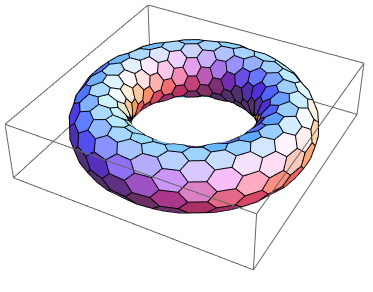
\includegraphics[width=0.75\textwidth]{images/test_image}
	\caption{Current Balance in a Tokamak} ~\\
	\small In a tokamak, there needs to be a certain amount of current -- and that current has to come from somewhere. All good reactors have an adequate bootstrap current. What provides the remaining current is what distinguishes steady state from pulsed operation.
	\label{fig:curbal}
\end{figure}

This equation shows how steady-state and pulsed operation can coexist (see \cref{fig:curbal}). The final point to make is reducing the model to being purely pulsed -- i.e.\ neglecting the current drive:
\begin{equation}
	1 = f_{BS} + f_{ID}
\end{equation}
Therefore, the next chapter will generalize the steady current to allow pulsed operation, and then simplify it to the purely pulsed case. Just as steady current faced self-consistency issues with $\eta_{CD}$, this current will also involve its own root solving conundrum -- the description of which will be given in the following two chapters.

\subsubsection{The Tokamak Magnet Strength -- $B_0$}

The tokamak magnet strength has no \replaced{unique}{obvious} equation to eliminate it. With foresight, the one this model \replaced{uses}{chooses to use} is \added{the} power balance \replaced{inherent to every}{in a} reactor. Similar to current balance, power balance is what separates a reactor from a \replaced{device incapable of producing net electricity}{toaster}. As such, it is referred throughout this document as: the primary constraint. It will be derived later this chapter.

\subsubsection{The Tokamak Major Radius -- $R_0$}

Much like the magnet strength, the major radius has no \replaced{unique}{obvious} relation to express it. \replaced{The model therefore uses this equation to handle a reactor's various}{This is convenient, because the model still has yet to resolve one of its most pressing issues:} physical and engineering-based constraints. This \deleted{laundry} list of requirements further restricts reactor space to the curves shown in the results section. Collectively, these are referred to as the \replaced{limiting}{secondary} constraints -- discussed later this chapter. \replaced{These}{By miracle, these} constraints all just happen to depend on the size of the reactor -- the reason they are chosen to \replaced{represent}{substitute out} the radius.

\section{Enforcing Power Balance}

What separates a reactor from a \replaced{device incapable of producing net electricity}{toaster} is power balance. \replaced{Within a tokamak, it}{It} accounts for how the power going into a plasma's core exactly matches the power coming out of it. To approximate this conservation equation, two sets of power will be introduced: the sources and the sinks. 

The sources have mainly been introduced at this point -- they include the alpha power ($P_\alpha$) \added{from fusion reactions} and the heating power ($P_H$), as well as a new ohmic power term ($P_\Omega$). The remaining two powers -- the sinks -- then appear through the radiation and heat conduction losses, which will be given shortly. In equation form, power balance becomes:
\begin{equation}
	\sum_{sources} P = \sum_{sinks} \, P
\end{equation}
or expanded to fit this model:
\begin{equation}
	\label{eq:power_balance}
	P_\alpha + P_H + P_\Omega = P_{BR} + P_\kappa
\end{equation}
For clarity, the left-hand side of this equality are the sources. Whereas the remaining two are sinks, i.e.\ Bremsstrahlung radiation ($P_{BR}$) and heat conduction losses ($P_\kappa$).

\subsection{Collecting Power Sources}

As suggested, the two dominant sources of power in a tokamak are: alpha power ($P_\alpha$) and auxiliary heating ($P_H$). From \cref{chapter:power}, it was determined that alpha particles (i.e.\ helium nuclei) carry around 20\% of the total fusion power; or as we put it mathematically:
\begin{equation}
	\label{eq:palpha}
	P_\alpha = \frac{P_F}{5}
\end{equation}
Additionally, it was determined that the heating power is what was eventually amplified into fusion power -- or through equation:
\begin{equation}
	\label{eq:ph}
	P_H = \frac{P_F}{Q}
\end{equation}
The final source term then is the ohmic power ($P_\Omega$). This is identical to how copper wires in a home heat up as current runs through them. From a simple circuits picture, the power across the plasma is related to its current and resistance -- in our standardized units -- through:
\begin{equation}
	\label{eq:pohmic_basic}
	P_\Omega = 10^6 \cdot I_P^2 \cdot R_P
\end{equation}
\deleted{Here, the resistance of the plasma is unlike any material humans encounter on a daily basis -- actually decreasing with temperature.} \replaced{This}{The} fusion systems model handles the plasma resistance ($R_P$)  with the neoclassical Spitzer resistivity. Through equation,\added{\cite{jeff}}
\begin{equation}
	\label{eq:rp}
	R_P = \frac{K_{RP}}{R_0 \overline T ^ {3/2}}
\end{equation}
\begin{equation}
	K_{RP} = 5.6e{-8} \cdot \left( \frac{ Z_{eff} }{ \epsilon^2 \kappa } \right) \cdot \left( \frac{1}{ 1 - 1.31 \sqrt{ \epsilon } + 0.46 \epsilon } \right)
\end{equation}

Combined with the Greenwald limit, ohmic power can be written more compactly as,
\begin{equation}
	\label{eq:pohmic}
	P_\Omega = K_\Omega \cdot \left( \frac{ \overline n ^ 2 R_0^3 }{\overline T ^ {3/2}} \right)
\end{equation}
\begin{equation}
	K_\Omega = 10^6 \cdot \frac{K_{RP}}{K_n^2}
\end{equation}
With the sources defined, we are now in a position to discuss the two sink terms used in this model's power balance.

\subsection{Approximating Radiation Losses}

All nuclear reactors emit radiation. From a power balance perspective, this means some power has to always be reserved to recoup from its losses -- measured in megawatts. In a fusion reactor, the three most important types of radiation are: Bremsstrahlung radiation, line radiation, and synchrotron radiation. 

\replaced{This}{Without going into too much detail, this} model chooses to only model Bremsstrahlung radiation -- as it usually dominates within the plasma's core. \added{Within most designs, Bremsstrahlung radiation outweighs the other two's contribution, to core power balance, two-to-one.\cite{ussteady,inputfile} } However, adding the effects of line-radiation and synchrotron radiation would drive results closer to real-world experiments. For example, line-radiation would better account for the \added{effects of} heavy impurities that \replaced{are emitted from the divertor plate and first wall}{appear as pieces of a tokamak fall into the plasma.}

For clarity, Bremsstrahlung -- or breaking -- radiation is what occurs when a charged particle (e.g.\ an electron) is accelerated by some means. In a tokamak, this happens all the time as \replaced{electrons collide with the ion species.\cite{hutch}}{charged particles are flung around and around the machine.} \replaced{This term can be}{As given in Jeff Freidberg's book, this term is} described by the volume integral:\added{\cite{jeff}}
\begin{equation}
	P_{BR} = \int S_{BR} \, d \vec{r}
\end{equation}

\replaced{Where}{Here,} the radiation power density ($S_{BR}$) is given by:
\begin{equation}
	S_{BR} = \left( \frac{\sqrt{2}}{3 \sqrt{\pi^5}} \cdot \frac{e^6}{\epsilon_0^2 c^3 h m_e^{3/2}} \right) \cdot \left( Z_{eff} \, n^2 \, T^{1/2} \right)
\end{equation}

The constants in the left set of parentheses all have their usual physics meanings (i.e.\ c is the speed of light and $m_e$ is the mass of an electron). What is new is the effective charge: $Z_{eff}$.

The effective charge is a scheme for \replaced{reducing}{collapsing} the charge \replaced{each ion}{that each particle} has to a \replaced{single representative}{collective} value. Fundamental charge, here, is what: neutrons lack, electrons and hydrogen have one of, and helium has two. As such, a plasma with a purely deuterium and tritium fuel would have an effective charge of one. This value would then quickly rise if a Tungsten tile -- with 74 units of charge -- were to fall into the plasma core from the walls of the tokamak.

Using the volume integral -- seen in the derivation of fusion power -- allows the Bremsstrahlung power to be written in standardized units as:
\begin{equation}
	\label{eq:pbr}
	P_{BR} = K_{BR} \ \overline n ^ 2 \ \overline T ^ {1/2} R_0^3 
\end{equation}
\begin{equation}
	K_{BR} = 0.1056 \, \frac{ (1+\nu_n)^2 \, (1+\nu_T)^{1/2} }{1+2 \, \nu_n + 0.5 \, \nu_T} \, Z_{eff} \, \epsilon^2 \, \kappa \, g
\end{equation}

This power term represents the radiation power losses involved in power balance. All that is needed now is a formula for heat conduction losses -- \replaced{one of the most difficult plasma behaviors}{the hardest plasma behavior} to model to date.

\subsection{Estimating Heat Conduction Losses}

Heat is energy that \replaced{moves about randomly}{lacks direction} on a microscopic level. Macroscopically, it generally moves from hotter areas to colder ones. As hinted by the plasma profile for temperature, heat emanates from the center of a plasma and migrates towards the walls of its tokamak enclosure. It therefore \replaced{is a critical}{seems an important} quantity to calculate when balancing power in a plasma's core.

The difficulty of estimating heat conduction, though, lies in the \replaced{nonlinear behaviors}{chaotic nature} of plasmas -- no theory or \replaced{quick-running code}{computation today} can properly model it. As such, reactor designers have turned towards experimentalists for empirical scaling laws based on the dozen or so strongest tokamaks in the world. These are collectively referred to as confinement time scalings, i.e.\ the ELMy H-Mode Scaling Law.

The derivation of this heat conduction loss term ($P_\kappa$) starts in a manner similar to the previous powers. To begin, an equation for $P_\kappa$ \replaced{can be found using the following volume integral:\cite{jeff}}{sis given in Jeff Freidberg's book as:} 
\begin{equation}
	P_\kappa = \frac{1}{\tau_E} \int U d \vec r
\end{equation}

This volume integral includes two new terms: the confinement time ($\tau_E$) and the internal energy (U). Before explaining these terms, a qualitative description is in order. As mentioned previously, the heat -- or microscopically random -- energy is captured by the internal energy (U). Then the confinement time ($\tau_E$) is how long it would take for the heat to \replaced{undergo an e-folding}{completely leave the device} if the \replaced{device}{system} were suddenly turned off.

A formula for confinement time will be delayed till the end of this section, when it is needed to solve for the magnetic field ($B_0$). The internal energy (U), however, can be given now as it has its typical physics meaning. This assumes that all three plasma species are held nearly at the same temperature (T) as the electrons:
\begin{equation}
	U = \frac{3}{2} \left( n + n_D + n_T \right) T
\end{equation}

Here again, $n_D$ and $n_T$ -- the density of deuterium and tritium, respectively -- are related to the electron density (used in this model) through the dilution factor, which assumes a 50-50 mix of D-T fuel:
\begin{equation}
	n_D = n_T = f_D \cdot \left( \, \frac{n}{2} \, \right)
\end{equation}

\replaced{After several substitutions,}{Foregoing the mathematical rigor of previous sections,} the equations here can be combined to form an equation for $P_\kappa$ -- the heat conduction losses -- in standardized units:
\begin{equation}
	\label{eq:pkappa}
	P_\kappa = K_\kappa \, \frac{ R_0 ^ 3 \ \overline{n}  \ \overline{T}  }{\tau_E} 
\end{equation}
\begin{equation}
	K_\kappa = 0.4744 \, ( 1 + f_D ) \, \frac{ (1 + \nu_n) \, (1 + \nu_T) }{1 + \nu_n + \nu_T } \, ( \, \epsilon^2 \, \kappa \, g \, )
\end{equation}

Now that all five terms have been defined in power balance, the next step is expanding it and solving for the tokamak's toroidal magnetic field strength: $B_0$.

\subsection{Writing the Lawson \replaced{Parameter}{Criterion}}

Before \replaced{arriving at a formula for}{locking in the primary constraint -- i.e.\ } the magnet strength ($B_0$) \replaced{using}{equation from} power \replaced{balance,}{balance} -- it seems appropriate to take a detour and explain an intermediate solution: the Lawson \replaced{Parameter}{Criterion}. Within the fusion community, the Lawson \replaced{Parameter}{Criterion} is the cornerstone in any argument on the possibility of a \replaced{tokamak ever}{design} being used as a \replaced{reactor.}{reactor (and not just some grandiose toaster).}

An equation for the Lawson \replaced{Parameter}{Criterion} -- sometimes referred to as the \emph{triple product} -- is easily found in the literature as:
\begin{equation}
	\label{eq:lawson}
	n \cdot T \cdot \tau_E = \frac{ 60 }{ E_F } \cdot \frac{ T ^ 2 }{ \langle \sigma v \rangle }
\end{equation}

Similar to the steady current derived earlier, the right-hand side is only dependent on temperature. Further, as the left-hand side is a measure of difficult to achieve parameters, the goal is to minimize both sides. \replaced{As shown in \cref{fig:lawson}, this}{This} occurs when the plasma temperature is around 15 keV -- a fact \replaced{well known to}{memorized by} many fusion engineers. As will be seen, this is a simplified result of our model. This is why $\overline T$ = 15 keV is not always the optimum temperature -- but usually is in the right neighborhood for reasonable reactor designs.

\begin{figure}
	\centering
	\begin{adjustbox}{width=0.75\textwidth}
		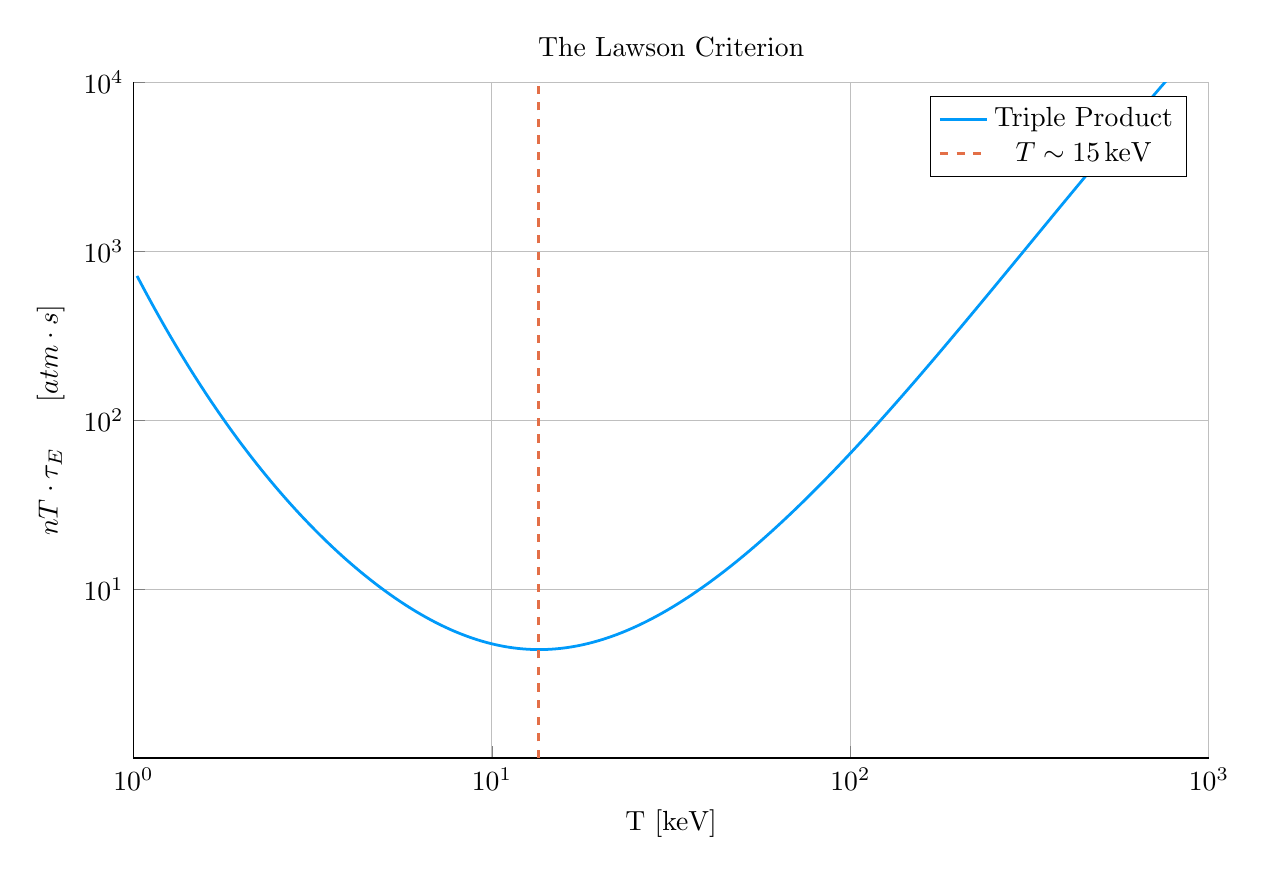
\begin{tikzpicture}[]
\begin{axis}[height = {101.6mm}, ylabel = {$n T \cdot \tau_E \ \ \ \ \ [atm \cdot s]$}, title = {The Lawson Criterion}, xmin = {1.0}, xmax = {1000.0}, ymax = {10000.0}, ymode = {log}, xlabel = {T   [keV]}, {unbounded coords=jump, xticklabel style={rotate = 0}, log basis x=10, xmajorgrids = true, xtick = {1.0,10.0,100.0,1000.0}, xticklabels = {$10^{0}$,$10^{1}$,$10^{2}$,$10^{3}$}, xtick align = inside, axis lines* = left, yticklabel style={rotate = 0}, log basis y=10, ymajorgrids = true, ytick = {10.0,100.0,1000.0,10000.0}, yticklabels = {$10^{1}$,$10^{2}$,$10^{3}$,$10^{4}$}, ytick align = inside, axis lines* = left,     xshift = 0.0mm,
    yshift = 0.0mm,
    axis background/.style={fill={rgb,1:red,1.00000000;green,1.00000000;blue,1.00000000}}
}, xmode = {log}, ymin = {1.001}, width = {152.4mm}]\addplot+ [color = {rgb,1:red,0.00000000;green,0.60560316;blue,0.97868012},
draw opacity=1.0,
line width=1,
solid,mark = none,
mark size = 2.0,
mark options = {
    color = {rgb,1:red,0.00000000;green,0.00000000;blue,0.00000000}, draw opacity = 1.0,
    fill = {rgb,1:red,0.00000000;green,0.60560316;blue,0.97868012}, fill opacity = 1.0,
    line width = 1,
    rotate = 0,
    solid
}]coordinates {
(1.023292992280754, 715.5843693055245)
(1.0471285480508996, 652.0764819850596)
(1.0715193052376064, 594.8592282501459)
(1.096478196143185, 543.2546522451097)
(1.1220184543019633, 496.663131536487)
(1.1481536214968828, 454.5537705698688)
(1.1748975549395295, 416.456035426309)
(1.202264434617413, 381.9524618339787)
(1.2302687708123816, 350.67229211863474)
(1.2589254117941673, 322.2859170225961)
(1.288249551693134, 296.50001561571264)
(1.318256738556407, 273.0533013093717)
(1.3489628825916535, 251.71279464231827)
(1.3803842646028848, 232.27055435304894)
(1.4125375446227544, 214.54080755655357)
(1.4454397707459274, 198.35742783107645)
(1.4791083881682074, 183.57171688596867)
(1.5135612484362082, 170.05045138851656)
(1.5488166189124815, 157.67416161454238)
(1.5848931924611136, 146.33561297294165)
(1.62181009735893, 135.9384652384002)
(1.6595869074375607, 126.3960875950959)
(1.6982436524617444, 117.63051042010802)
(1.7378008287493754, 109.57149718083319)
(1.7782794100389228, 102.155721939162)
(1.8197008586099834, 95.32603979193581)
(1.8620871366628675, 89.03083917128589)
(1.9054607179632472, 83.22346631314609)
(1.9498445997580451, 77.86171340616474)
(1.9952623149688795, 72.90736298097448)
(2.041737944669529, 68.32578201236458)
(2.0892961308540396, 64.08556000253319)
(2.137962089502232, 60.158186007840044)
(2.1877616239495525, 56.51776017780416)
(2.2387211385683394, 53.14073590510077)
(2.290867652767773, 50.0056891489945)
(2.344228815319922, 47.093111900666955)
(2.3988329190194904, 44.38522711472284)
(2.4547089156850306, 41.86582274326229)
(2.51188643150958, 39.52010278288166)
(2.5703957827688635, 37.33455348568332)
(2.6302679918953817, 35.29682309703734)
(2.6915348039269156, 33.395613669101465)
(2.7542287033381663, 31.62058366316803)
(2.8183829312644537, 29.962260198507185)
(2.884031503126606, 28.411959932944896)
(2.9512092266663856, 26.961717673034713)
(3.019951720402016, 25.60422191119189)
(3.0902954325135905, 24.332756575143232)
(3.1622776601683795, 23.141148352912094)
(3.2359365692962827, 22.0237190255119)
(3.311311214825911, 20.975242300634317)
(3.3884415613920256, 19.990904694824255)
(3.4673685045253166, 19.066270059743925)
(3.548133892335755, 18.197247390865947)
(3.630780547701014, 17.380061594923447)
(3.715352290971725, 16.611226926240565)
(3.8018939632056115, 15.887522832148305)
(3.890451449942806, 15.205971974493213)
(3.9810717055349722, 14.563820218135483)
(4.073802778041127, 13.9585183986498)
(4.168693834703354, 13.387705700467096)
(4.265795188015927, 12.849194493696395)
(4.36515832240166, 12.340956493058842)
(4.466835921509632, 11.86111011596177)
(4.570881896148751, 11.407908928906801)
(4.677351412871983, 10.979731082327069)
(4.786300923226384, 10.575069643717114)
(4.897788193684462, 10.192523747682124)
(5.011872336272722, 9.830790489396893)
(5.1286138399136485, 9.4886574950276)
(5.248074602497725, 9.16499610901522)
(5.370317963702527, 8.858755143826464)
(5.495408738576246, 8.568955142911767)
(5.623413251903491, 8.29468311223238)
(5.7543993733715695, 8.035087679882023)
(5.88843655355589, 7.789374647081937)
(6.025595860743578, 7.556802897213308)
(6.165950018614822, 7.336680632605374)
(6.309573444801933, 7.1283619115573345)
(6.456542290346556, 6.931243460563939)
(6.606934480075959, 6.7447617389697925)
(6.760829753919817, 6.5683902353161425)
(6.918309709189364, 6.4016369764913525)
(7.079457843841379, 6.244042232468866)
(7.244359600749901, 6.095176400934137)
(7.413102413009175, 5.954638057478739)
(7.5857757502918375, 5.822052158290098)
(7.762471166286917, 5.697068383402136)
(7.943282347242816, 5.579359609605691)
(8.128305161640993, 5.4686205030596)
(8.31763771102671, 5.364566222501177)
(8.511380382023766, 5.266931224738075)
(8.709635899560805, 5.175468164818683)
(8.912509381337454, 5.089946883932297)
(9.120108393559097, 5.010153478689247)
(9.33254300796991, 4.93588944597961)
(9.549925860214358, 4.866970898113729)
(9.772372209558107, 4.803227843409827)
(10.0, 4.74450352782116)
(10.232929922807541, 4.690653833587014)
(10.471285480508996, 4.641546731255455)
(10.715193052376065, 4.597061781760152)
(10.964781961431852, 4.557089685544928)
(11.220184543019636, 4.521531876017525)
(11.481536214968829, 4.490300154882151)
(11.748975549395297, 4.463316367150074)
(12.02264434617413, 4.4405121138606)
(12.302687708123818, 4.4218285007630715)
(12.589254117941675, 4.407215921415124)
(12.882495516931343, 4.39663387334517)
(13.182567385564074, 4.390050806109046)
(13.489628825916533, 4.38744400024263)
(13.803842646028846, 4.388799476276163)
(14.12537544622754, 4.3941119331320175)
(14.454397707459272, 4.403384715376948)
(14.791083881682072, 4.416629808943959)
(15.13561248436208, 4.433867865077917)
(15.488166189124811, 4.455128252393695)
(15.848931924611133, 4.48044913706814)
(16.218100973589298, 4.509877591315835)
(16.595869074375607, 4.5434697304270015)
(16.982436524617444, 4.581290878772013)
(17.378008287493753, 4.6234157653040935)
(17.78279410038923, 4.669928749218003)
(18.197008586099834, 4.72092407655112)
(18.620871366628677, 4.7765061686425785)
(19.054607179632473, 4.836789943498778)
(19.498445997580454, 4.9019011712485865)
(19.952623149688797, 4.971976865010962)
(20.417379446695296, 5.047165708641305)
(20.892961308540396, 5.127628522971638)
(21.379620895022324, 5.213538772314609)
(21.87761623949553, 5.305083113162599)
(22.3872113856834, 5.4024619871819475)
(22.908676527677734, 5.505890260779421)
(23.442288153199225, 5.615597913703399)
(23.9883291901949, 5.73183077933847)
(24.547089156850298, 5.854851339557513)
(25.118864315095795, 5.984939577213792)
(25.703957827688633, 6.122393889584756)
(26.302679918953814, 6.267532066323497)
(26.915348039269155, 6.420692335730828)
(27.542287033381662, 6.582234483434617)
(28.183829312644534, 6.752541047852738)
(28.84031503126606, 6.932018597123181)
(29.512092266663856, 7.121099092511616)
(30.19951720402016, 7.3202413436533345)
(30.902954325135905, 7.52993256135462)
(31.622776601683793, 7.750690014070107)
(32.359365692962825, 7.983062794588698)
(33.11311214825911, 8.227633703902626)
(33.884415613920254, 8.485021259704226)
(34.673685045253166, 8.75588183745494)
(35.48133892335755, 9.040911952501903)
(36.30780547701014, 9.340850692282585)
(37.15352290971726, 9.656482308258274)
(38.018939632056124, 9.988638977855283)
(38.90451449942807, 10.33820374737135)
(39.810717055349734, 10.706113667526031)
(40.73802778041128, 11.093363134099329)
(41.68693834703355, 11.50100744691819)
(42.65795188015925, 11.930166601314705)
(43.65158322401658, 12.382029327098968)
(44.6683592150963, 12.857857391065538)
(45.708818961487495, 13.358990180088743)
(46.77351412871981, 13.886849582961755)
(47.86300923226383, 14.442945190302456)
(48.97788193684461, 15.028879833087446)
(50.11872336272722, 15.646355481690618)
(51.28613839913648, 16.297179528695864)
(52.48074602497726, 16.983271480232325)
(53.70317963702527, 17.706670082146438)
(54.954087385762456, 18.469540908986364)
(56.23413251903491, 19.274184445531887)
(57.543993733715695, 20.1230446924667)
(58.8843655355589, 21.01871832976149)
(60.25595860743578, 21.963964473423015)
(61.65950018614822, 22.96171506347328)
(63.09573444801933, 24.015085923357283)
(64.56542290346556, 25.127388533447483)
(66.06934480075961, 26.302142563921986)
(67.60829753919819, 27.543089215049925)
(69.18309709189366, 28.85420541582856)
(70.79457843841381, 30.2397189349887)
(72.44359600749902, 31.704124461627565)
(74.13102413009177, 33.25220071614717)
(75.85775750291836, 34.889028655780834)
(77.62471166286916, 36.620010842788844)
(79.43282347242814, 38.45089204740532)
(81.2830516164099, 40.387781161829686)
(83.17637711026708, 42.43717450598852)
(85.11380382023764, 44.6059806104552)
(87.09635899560806, 46.90154656681403)
(89.12509381337455, 49.331686040906135)
(91.20108393559097, 51.90470904980014)
(93.3254300796991, 54.62945360900688)
(95.49925860214358, 57.515319362410956)
(97.72372209558107, 60.57230331363601)
(100.0, 63.81103778410115)
(102.32929922807536, 67.24283072987917)
(104.71285480508996, 70.87970855663967)
(107.1519305237606, 74.73446157946178)
(109.64781961431851, 78.82069228215158)
(112.2018454301963, 83.15286653889214)
(114.81536214968828, 87.74636796962139)
(117.48975549395291, 92.61755560946783)
(120.22644346174131, 97.78382508189834)
(123.02687708123811, 103.26367347494983)
(125.89254117941675, 109.07676813004912)
(128.82495516931337, 115.24401956346287)
(131.82567385564073, 121.78765875140567)
(134.89628825916532, 128.7313190212372)
(138.03842646028852, 136.10012280306256)
(141.2537544622754, 143.92077350836064)
(144.5439770745928, 152.22165281508785)
(147.91083881682073, 161.03292365197024)
(151.35612484362088, 170.38663918850096)
(154.88166189124811, 180.3168581514265)
(158.48931924611142, 190.859766803331)
(162.18100973589299, 202.05380793424246)
(165.95869074375614, 213.93981723308698)
(169.82436524617444, 226.5611674222155)
(173.78008287493762, 239.96392055525848)
(177.82794100389228, 254.19698889610504)
(181.97008586099827, 269.3123048150095)
(186.20871366628674, 285.3650001565748)
(190.54607179632464, 302.41359555379074)
(194.98445997580455, 320.5202001823509)
(199.52623149688787, 339.75072247016425)
(204.17379446695296, 360.175092298409)
(208.92961308540387, 381.86749525252964)
(213.79620895022325, 404.9066195044671)
(218.77616239495518, 429.37591593094083)
(223.872113856834, 455.36387209705316)
(229.08676527677724, 482.9643007596241)
(234.42288153199226, 512.2766435708044)
(239.88329190194898, 543.4062906894171)
(245.4708915685031, 576.464917035484)
(251.18864315095797, 611.5708359522358)
(257.03957827688646, 648.8493710699868)
(263.02679918953817, 688.4332471972791)
(269.1534803926917, 730.4630010970918)
(275.4228703338166, 775.087413039401)
(281.8382931264455, 822.4639600564246)
(288.40315031266056, 872.7592918631268)
(295.1209226666387, 926.1497304436313)
(301.9951720402016, 982.8217943436637)
(309.0295432513592, 1042.972748750622)
(316.22776601683796, 1106.8111824860716)
(323.5936569296281, 1174.5576130809143)
(331.1311214825911, 1246.4451211509213)
(338.84415613920237, 1322.7200153403764)
(346.73685045253166, 1403.6425291540393)
(354.8133892335753, 1489.4875510528248)
(363.0780547701014, 1580.545389247023)
(371.5352290971724, 1677.1225726820153)
(380.1893963205613, 1779.542689776586)
(389.04514499428046, 1888.147266542193)
(398.1071705534973, 2003.2966857842675)
(407.3802778041126, 2125.3711491630897)
(416.8693834703355, 2254.771683973346)
(426.57951880159254, 2391.92119658728)
(436.5158322401661, 2537.2655745980082)
(446.683592150963, 2691.2748397961623)
(457.0881896148752, 2854.4443542162185)
(467.73514128719813, 3027.296081597634)
(478.6300923226385, 3210.379906722357)
(489.77881936844614, 3404.2750152128565)
(501.18723362727246, 3609.591336506103)
(512.8613839913648, 3826.971052857308)
(524.8074602497728, 4057.0901773752544)
(537.0317963702527, 4300.660204247052)
(549.5408738576248, 4558.429834477045)
(562.341325190349, 4831.186780640399)
(575.4399373371566, 5119.759654339896)
(588.843655355589, 5425.019940252352)
(602.5595860743575, 5747.884060862276)
(616.5950018614822, 6089.315536203627)
(630.957344480193, 6450.327243166718)
(645.6542290346556, 6831.983779178804)
(660.6934480075957, 7235.403935331275)
(676.0829753919819, 7661.763284308377)
(691.8309709189363, 8112.296888768487)
(707.945784384138, 8588.302136144339)
(724.4359600749899, 9091.141706159546)
(741.3102413009177, 9622.24667771128)
(758.5775750291835, 10183.11978213795)
(776.247116628692, 10775.338810284076)
(794.3282347242813, 11400.560181185736)
(812.8305161640995, 12060.52268063764)
(831.7637711026708, 12757.051378360826)
(851.1380382023768, 13492.06173297636)
(870.9635899560806, 14267.563894499495)
(891.2509381337459, 15085.667214609008)
(912.0108393559096, 15948.584975511469)
(933.2543007969915, 16858.63934881972)
(954.992586021436, 17818.266596491703)
(977.2372209558112, 18830.022526540524)
(1000.0, 19896.588216921093)
(1023.2929922807537, 21020.77602173607)
(1047.1285480508996, 22205.535874673045)
(1071.519305237606, 23453.961905400487)
(1096.4781961431852, 24769.29938550517)
(1122.018454301963, 26154.952021453166)
(1148.1536214968828, 27614.489613007096)
(1174.897554939529, 29151.656096526574)
(1202.2644346174131, 30770.37799363245)
(1230.268770812381, 32474.77328681697)
(1258.9254117941675, 34269.16074474929)
(1288.2495516931335, 36158.06972124623)
(1318.2567385564075, 38146.2504531722)
(1348.9628825916532, 40238.68488388557)
(1380.3842646028852, 42440.598040283076)
(1412.537544622754, 44757.46999299408)
(1445.439770745928, 47195.048430870826)
(1479.1083881682073, 49759.3618825815)
(1513.5612484362086, 52456.73361988538)
(1548.816618912481, 55293.79627901266)
(1584.893192461114, 58277.5072385393)
(1621.8100973589299, 61415.16479419626)
(1659.5869074375614, 64714.42517323727)
(1698.2436524617442, 68183.3204332687)
(1737.8008287493763, 71830.27729287352)
(1778.2794100389228, 75664.13694389607)
(1819.7008586099826, 79694.17589795444)
(1862.0871366628676, 83930.12792257269)
(1905.4607179632462, 88382.20712532024)
(1949.8445997580454, 93061.13224750487)
(1995.2623149688789, 97978.15223228547)
(2041.7379446695295, 103145.07313560059)
(2089.296130854039, 108574.28645200086)
(2137.9620895022326, 114278.79893140584)
(2187.761623949552, 120272.26396692236)
(2238.72113856834, 126569.01463824147)
(2290.8676527677726, 133184.09849971998)
(2344.228815319923, 140133.3142071364)
(2398.83291901949, 147433.25008222583)
(2454.708915685031, 155101.32471954415)
(2511.88643150958, 163155.82974591767)
(2570.3957827688646, 171615.97484880453)
(2630.2679918953813, 180501.9351962624)
(2691.5348039269165, 189834.9013779866)
(2754.2287033381663, 199637.13200398907)
(2818.382931264455, 209932.00910503615)
(2884.031503126606, 220744.09648690396)
(2951.209226666387, 232099.20119892008)
(3019.9517204020162, 244024.43828613157)
(3090.295432513592, 256548.29900382337)
(3162.2776601683795, 269700.72268301074)
(3235.936569296281, 283513.1724460091)
(3311.311214825911, 298018.714982234)
(3388.441561392024, 313252.1046060778)
(3467.368504525317, 329249.87183106877)
(3548.133892335753, 346050.41670754453)
(3630.780547701014, 363694.1071848948)
(3715.352290971724, 382223.3827739712)
(3801.8939632056126, 401682.863800698)
(3890.4514499428046, 422119.46655815904)
(3981.0717055349733, 443582.52468168386)
(4073.802778041126, 466123.9170895939)
(4168.693834703355, 489798.2028515374)
(4265.795188015925, 514662.763366615)
(4365.158322401661, 540777.9522550126)
(4466.835921509631, 568207.2533895164)
(4570.881896148751, 597017.4475173334)
(4677.351412871981, 627278.7879479581)
(4786.300923226385, 659065.1858096905)
(4897.7881936844615, 692454.4054057244)
(5011.872336272725, 727528.2702307551)
(5128.613839913648, 764372.8802406823)
(5248.074602497728, 803078.841001585)
(5370.317963702527, 843741.5053794787)
(5495.408738576249, 886461.2284699624)
(5623.413251903491, 931343.6365063301)
(5754.399373371566, 978499.910526803)
(5888.43655355589, 1.0280470856256834e6)
(6025.595860743575, 1.080108366660198e6)
(6165.9500186148225, 1.1348134613343545e6)
(6309.57344480193, 1.1922989316334699e6)
(6456.542290346556, 1.252708564638612e6)
(6606.934480075957, 1.3161937638086632e6)
(6760.829753919818, 1.3829139618799328e6)
(6918.309709189362, 1.4530370565986685e6)
(7079.457843841381, 1.52673987057139e6)
(7244.359600749898, 1.6042086365912505e6)
(7413.102413009177, 1.6856395098764265e6)
(7585.775750291836, 1.771239108738555e6)
(7762.4711662869195, 1.8612250852863907e6)
(7943.282347242814, 1.955826727861547e6)
(8128.305161640995, 2.0552855970008024e6)
(8317.63771102671, 2.1598561968221436e6)
(8511.380382023768, 2.2698066838408946e6)
(8709.635899560806, 2.385419615337356e6)
(8912.509381337459, 2.506992739519579e6)
(9120.108393559096, 2.6348398298537624e6)
(9332.543007969914, 2.7692915660716193e6)
(9549.92586021436, 2.910696464508343e6)
(9772.372209558112, 3.0594218605781165e6)
(10000.0, 3.2158549463557494e6)
};
\addlegendentry{Triple Product}
\addplot+ [color = {rgb,1:red,0.88887350;green,0.43564919;blue,0.27812294},
draw opacity=1.0,
line width=1,
dashed,mark = none,
mark size = 2.0,
mark options = {
    color = {rgb,1:red,0.00000000;green,0.00000000;blue,0.00000000}, draw opacity = 1.0,
    fill = {rgb,1:red,0.88887350;green,0.43564919;blue,0.27812294}, fill opacity = 1.0,
    line width = 1,
    rotate = 0,
    solid
}]coordinates {
(13.489628825916533, 1.0)
(13.489628825916533, 10000.0)
};
\addlegendentry{$T \sim 15 \, \textnormal{keV}$}
\end{axis}

\end{tikzpicture}

	\end{adjustbox}
%	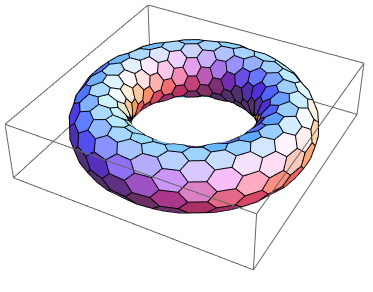
\includegraphics[width=0.75\textwidth]{images/test_image}
	\caption{Power Balance in a Reactor} ~\\
	\small Power balance is what differentiates a reactor from a radiator. When cast as the Lawson \replaced{Parameter}{Criterion} for fusion, it explains why D-T plasmas often have a temperature around 15 keV.
	\label{fig:lawson}
\end{figure}

As all the terms in power balance have already been defined, the starting point will be simply repeating the standardized equations for all five included powers.
\begin{equation}
	\tag{\ref{eq:palpha}}
	P_\alpha = \frac{P_F}{5}
\end{equation}
\begin{equation}
	\tag{\ref{eq:ph}}
	P_H = \frac{P_F}{Q}
\end{equation}
\begin{equation}
	\tag{\ref{eq:pohmic}}
	P_\Omega = K_\Omega \cdot \left( \frac{ \overline n ^ 2 R_0^3 }{\overline T ^ {3/2}} \right)
\end{equation}
\begin{equation}
	\tag{\ref{eq:pbr}}
	P_{BR} = K_{BR} \ \overline n ^ 2 \ \overline T ^ {1/2} R_0^3 
\end{equation}
\begin{equation}
	\tag{\ref{eq:pkappa}}
	P_\kappa = K_\kappa \, \frac{ R_0 ^ 3 \ \overline{n}  \ \overline{T}  }{\tau_E} 
\end{equation}

With the fusion power again being,
\begin{equation}
	\tag{\ref{eq:pf}}
	P_F = K_F \cdot \overline{n}^2 \cdot R_0^3  \cdot (\sigma v)
\end{equation}
These can then be substituted into power balance:
\begin{equation}
	\tag{\ref{eq:power_balance}}
	P_\alpha + P_H + P_\Omega = P_{BR} + P_\kappa
\end{equation}
After a couple lines of algebra, power balance can be rewritten in a form analogous to the triple product:
\begin{equation}
	\label{eq:ntaue}
	 \overline{n}  \cdot \overline{T} \cdot \tau_E = \frac{ K_\kappa \, \overline{T}^{\,2} }{ \left( K_P \, (\sigma v) +  K_{OH} \, \overline{T}^{  \,-3/2 } \right) - K_{BR} \, \overline{T}^{  \,1/2 } }
\end{equation}
\begin{equation}
	K_P = K_F \cdot \left( \frac{5 + Q}{5 \times Q} \right)
\end{equation}
\replaced{As expected, this shares a form}{As can be seen, this is remarkably} similar to the simple Lawson \replaced{Parameter}{Criterion}:
\begin{equation}
	\tag{\ref{eq:lawson}}
	n \cdot T \cdot \tau_E = \frac{ 60 }{ E_F } \cdot \frac{ T ^ 2 }{ \langle \sigma v \rangle }
\end{equation} 
The main difference is this model does not ignore ohmic power and radiation losses completely. The inclusion of radiation for example sometimes bars a range of temperatures from being physically realizable.\footnote{ The denominator of Eq \ref{eq:ntaue} has discontinuities when the $K_{BR} \, \overline{T}^{  \,1/2 }$ term exactly equals the parenthesised one. Therefore, valid reactors only exist outside the discontinuities, when the entire triple product is finite and positive. } With this intermediate relation in place, the goal is now to give a formula for the confinement time and solve it for the magnetic field strength ($B_0$) -- thus giving the Primary Constraint.

\subsection{Finalizing the Primary Constraint}

The goal now is to transform the Lawson \replaced{Parameter}{Criterion} into an equation for magnet strength ($B_0$). This choice to solve the equation for $B_0$ was \replaced{motivated by the goals of analysis and how it will fit}{completely arbitrary, only motivated by the foresight of how it fits} into the fusion systems model. To solve the primary constraint, the confinement time scaling law will need to be introduced. At the end, a \replaced{convoluted}{messy} -- albeit highly useful -- relation will be the reward.

The energy confinement time -- $\tau_E$ -- is one of the most \replaced{difficult to obtain}{elusive} terms in all of fusion energy. It is an attempt to \replaced{reduce}{boil down} all the \replaced{nonlinear behaviors}{chaotic nature} of plasmas into a simple measure of how fast its internal energy would be ejected from the tokamak if the device was instantaneously shut down. As such, reactor designers have turned toward experimentalists for empirical scalings based on the world's tokamaks. These all share a form similar to:
\begin{equation}
	\tau_E = K_\tau \, H \, \frac{
		I_P^{\,\alpha_I} \, R_0^{\,\alpha_R} \, a^{\,\alpha_a} \, \kappa^{\,\alpha_\kappa} \ \overline{n}^{\,\alpha_n} \, B_0^{\,\alpha_B} \, A^{\,\alpha_A}
	}{ P_{src} ^ {\,\alpha_P} }
	\label{eq:tau_gen}
\end{equation}
This \replaced{regressional fit}{mouthful of a formula} is how the field actually designs machines (i.e.\ ITER). Let it be known, though, that \replaced{fits of this kind}{these fits} often do remarkable well, having relative errors less than 20\% on interpolated data. The new terms in this equation are: $P_{src}$, $K_\tau$, H, A, and the $\alpha_{\,\square}$ factors. 

First, the loss power is a metric used in the engineering community to quantify the power being transported out of the ``core'' of the plasma by charged particles (i.e.\ not the neutrons). \cite{process} To optimize fits, experimentalists have defined this as a combination of the source power terms:
\begin{equation}
	\label{eq:pl}
	P_{src} = P_\alpha + P_H + P_\Omega
\end{equation}
\deleted{However, many have argued that the term should actually be replaced by its correct physics meaning -- the conductive heat loss power. As this model uses the ELMy H-Mode scaling law, which is standard in the field, this alternative definition will not be used:}
%\begin{equation}
%	\tilde P_{src} \approx P_\kappa = P_\alpha + P_H + P_\Omega - P_{BR}
%\end{equation}
Moving on, $K_\tau$ is simply a constant fit-makers use in their scalings. Whereas H is the \replaced{enhancement factor over the empirical fit.}{(H-Mode) scaling factor -- the analogue of $K_\tau$ used by reactor designers. This H factor can be used to artificially boost the confinement of a machine (i.e.\ it adds a little bit of magic).} \replaced{Next,}{Continuing,} A is the average mass number of the fuel source, in atomic mass units. For a 50-50 D-T fuel, this is 2.5, as deuterium weighs two amus and tritium weighs three. Lastly, the alpha factors (e.g.\ $\alpha_n$, $\alpha_a$, $\alpha_P$) are fitting parameters that represent each variable's relative importance in the scaling. 

For ELMy H-Mode, this confinement scaling law can be written as:
\begin{equation}
	\tau_E = 0.145 \, H \, \frac{
		I_P^{0.93} \, R_0^{1.39} \, a^{0.58} \, \kappa^{0.78} \ \overline{n}^{\, 0.41} \, B_0^{0.15} \, A^{0.19}
	}{ P_{src} ^ {\,0.69} }
	\label{eq:tau_h}
\end{equation}
\replaced{However, similar scaling laws}{Where similar ones} can be \replaced{written}{given} for L-Mode, I-Mode, etc. One final remark to make before moving on is that even these fits have subtleties. The value of $\kappa$, for example, may have a slightly different geometric meaning from tokamak to tokamak. And the exact definition of loss power -- $P_{src}$ -- introduces an even larger area of discrepancy.  \deleted{Although not actually used, a better fit for our model might be one from the author:}
%\begin{equation}
%	\tilde \tau_E = 0.08 \, H \frac{  
%		\left( R_0^{1.49} B_0 ^ {0.3} I_P^{0.93} \right) \cdot \left( \epsilon ^ {0.17} A^{0.23}  \kappa ^ {0.56} \right) }{ \tilde P_{src} ^ {\, 0.54} }	
%\end{equation}

Returning to the problem at hand, though, this model's Lawson \replaced{Parameter}{Criterion} (eq. \ref{eq:ntaue}) can be simplified after expanding the left-hand side using the Greenwald density and substituting in a confinement time scaling law. \replaced{After a few lines of algebra, this can be transformed}{Albeit a little cumbersome, this can be wrangled} into \replaced{a formula}{an equation} for $B_0$!
\begin{equation}
	\label{eq:b_0_power}
	\tcbhighmath{
	B_0 = \left( \frac{ G_{PB} }{ K_{PB} } \cdot \left( I_P^{\,\alpha_I^*} \, R_0^{ \alpha_R^* } \right)^{-1} \right) ^ { \frac{1}{ \alpha_B } }
	}
\end{equation}
\begin{equation}
	G_{PB} = \frac{ \overline{T} \cdot \left( \, K_P (\sigma v) + K_\Omega  \, \overline{T}^{  \,-3/2 } \, \right) ^ { \alpha_P } }{ \left( \, K_P (\sigma v) + K_\Omega  \, \overline{T}^{  \,-3/2 } - K_{BR} \, \overline{T}^{  \,1/2 } \, \right) }
\end{equation}
\begin{equation}
	K_{PB} = H \cdot \left( \frac{ K_\tau K_n^{\alpha_n^*}}{K_\kappa } \right) \cdot \left( 
     \epsilon^{\,\alpha_a} \, \kappa^{\,\alpha_\kappa} \, A^{\,\alpha_A}\right)
\end{equation}

Where we have added new starred alpha values for the density, current, and major radius:
\begin{equation}
  \alpha_n^* = 1 + \alpha_n - 2 \alpha_P
\end{equation}
\begin{equation}
  \alpha_I^* = \alpha_I + \alpha_n^*
\end{equation}
\begin{equation}
  \alpha_R^* = \alpha_R + \alpha_a - 2  \alpha_n^* - 3 \alpha_p
\end{equation}

\deleted{Again, if the alternate definition for heat loss ($\tilde P_{abs}$) were used, another definition for $G_{PB}$ would arise. Quickly reemphasizing, though, these tilded values are not actually used in the model:}
%\begin{equation}
%	\tilde G_{PB} = \frac{ \overline{T} }{ \left( \, K_P (\sigma v) + K_\Omega  \, \overline{T}^{  \,-3/2 } - K_{BR} \, \overline{T}^{  \,1/2 } \, \right) ^ { ( 1 - \alpha_P ) } }
%\end{equation}

This equation for $B_0$ -- derived from power balance -- is thus the primary constraint for reactor designs. It is the first step in connecting the plasma (i.e.\ $\overline n$, $\overline T$, and $I_P$) to its tokamak enclosure (i.e.\ $B_0$ and $R_0$). The remaining step is finding an equation -- or in this case, equations -- for the major radius of the device. These radius equations will collectively be referred to as: the \replaced{limiting constraints.}{Secondary Constraints.}

%\subsection{Exploring the Freidberg Criterion}

\deleted{Before moving onto the Secondary Constraint, it is worth noting that this power balance equation can be written in a triple product form analogous to the Lawson \replaced{Parameter}{Criterion}. For this reason, we will refer to it as the Freidberg Triple Product:}
%\begin{equation}
%	\label{eq:freidberg}
%	R_0^{ \alpha_R^* } \cdot B_0^{\,\alpha_B} \cdot I_P^{\,\alpha_I^*} = \frac{ G_{PB} }{ K_{PB} }
%\end{equation}

%\begin{figure*}[h]
%    \centering
%    \hfill 
%    \begin{subfigure}[t]{0.45\textwidth}
%        \centering
%		\begin{adjustbox}{width=\textwidth}
%			\Large
%			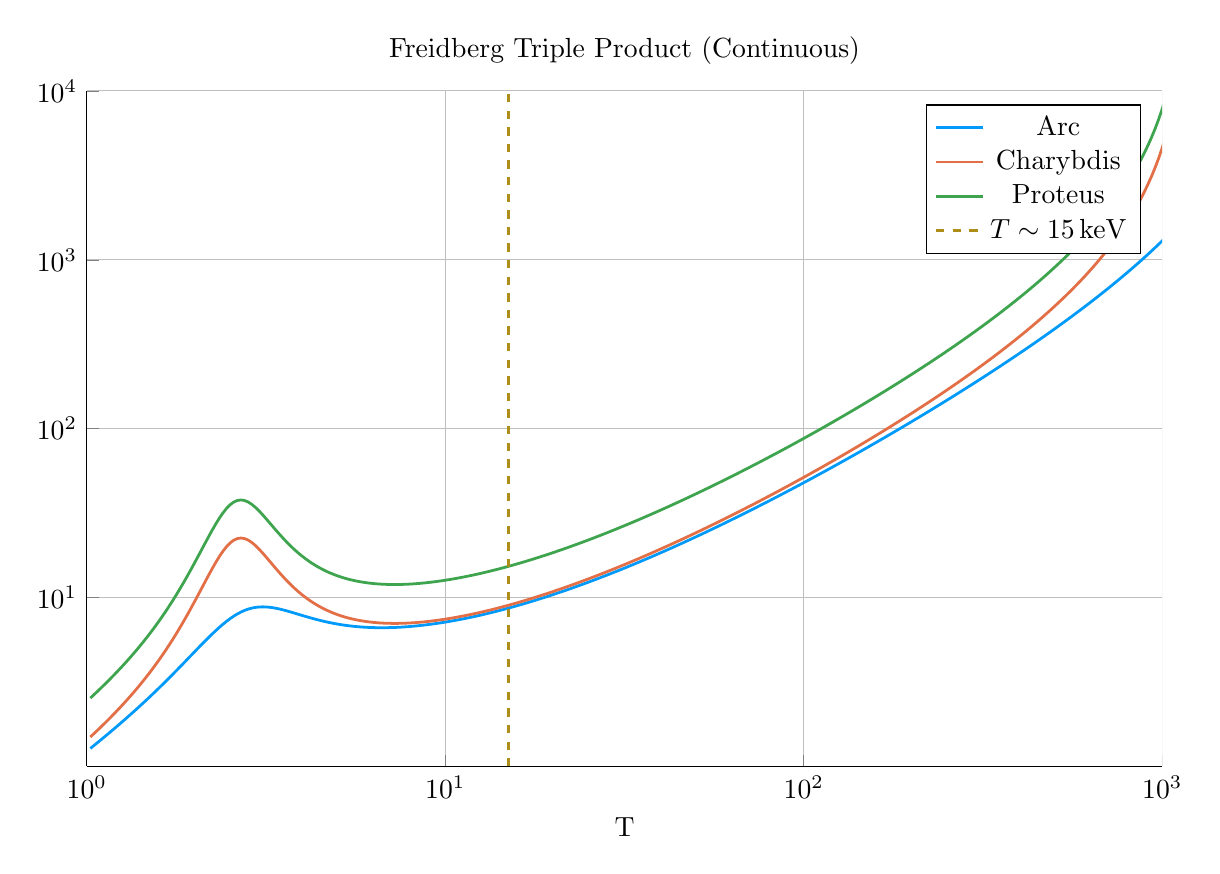
\begin{tikzpicture}[]
\begin{axis}[height = {101.6mm}, ylabel = {}, title = {Freidberg Triple Product (Continuous)}, xmin = {1.0}, xmax = {1000.0}, ymax = {10000.0}, ymode = {log}, xlabel = {T}, {unbounded coords=jump, xticklabel style={rotate = 0}, log basis x=10, xmajorgrids = true, xtick = {1.0,10.0,100.0,1000.0}, xticklabels = {$10^{0}$,$10^{1}$,$10^{2}$,$10^{3}$}, xtick align = inside, axis lines* = left, yticklabel style={rotate = 0}, log basis y=10, ymajorgrids = true, ytick = {10.0,100.0,1000.0,10000.0}, yticklabels = {$10^{1}$,$10^{2}$,$10^{3}$,$10^{4}$}, ytick align = inside, axis lines* = left,     xshift = 0.0mm,
    yshift = 0.0mm,
    axis background/.style={fill={rgb,1:red,1.00000000;green,1.00000000;blue,1.00000000}}
}, xmode = {log}, ymin = {1.001}, width = {152.4mm}]\addplot+ [color = {rgb,1:red,0.00000000;green,0.60560316;blue,0.97868012},
draw opacity=1.0,
line width=1,
solid,mark = none,
mark size = 2.0,
mark options = {
    color = {rgb,1:red,0.00000000;green,0.00000000;blue,0.00000000}, draw opacity = 1.0,
    fill = {rgb,1:red,0.00000000;green,0.60560316;blue,0.97868012}, fill opacity = 1.0,
    line width = 1,
    rotate = 0,
    solid
}]coordinates {
(1.023292992280754, 1.2793221218652944)
(1.0471285480508996, 1.3309195883591072)
(1.0715193052376064, 1.3850036910515204)
(1.096478196143185, 1.4417288746419747)
(1.1220184543019633, 1.5012617022690462)
(1.1481536214968828, 1.5637819142077942)
(1.1748975549395295, 1.6294835657026674)
(1.202264434617413, 1.698576242531264)
(1.2302687708123816, 1.7712863496330842)
(1.2589254117941673, 1.8478584635873476)
(1.288249551693134, 1.928556733480841)
(1.318256738556407, 2.0136663062561424)
(1.3489628825916535, 2.103494741323413)
(1.3803842646028848, 2.1983733642456036)
(1.4125375446227544, 2.2986584896716016)
(1.4454397707459274, 2.4047324181909375)
(1.4791083881682074, 2.5170040789980095)
(1.5135612484362082, 2.635909148564986)
(1.5488166189124815, 2.7619094231676584)
(1.5848931924611136, 2.8954911583354357)
(1.62181009735893, 3.0371620095937497)
(1.6595869074375607, 3.1874461154129454)
(1.6982436524617444, 3.3468767556900265)
(1.7378008287493754, 3.515985900410607)
(1.7782794100389228, 3.6952898405140475)
(1.8197008586099834, 3.8852699797335295)
(1.8620871366628675, 4.08634778460181)
(1.9054607179632472, 4.298852874384422)
(1.9498445997580451, 4.5229833332653655)
(1.9952623149688795, 4.758757610889229)
(2.041737944669529, 5.005957927860106)
(2.0892961308540396, 5.264066012456858)
(2.137962089502232, 5.532193347327445)
(2.1877616239495525, 5.809009942726736)
(2.2387211385683394, 6.092677927494796)
(2.290867652767773, 6.380798757486339)
(2.344228815319922, 6.670385163416938)
(2.3988329190194904, 6.957870427901035)
(2.4547089156850306, 7.239167326284057)
(2.51188643150958, 7.509786194163538)
(2.5703957827688635, 7.7650155007458315)
(2.6302679918953817, 8.000159131951143)
(2.6915348039269156, 8.210813513493981)
(2.7542287033381663, 8.393157056383407)
(2.8183829312644537, 8.544217197329235)
(2.884031503126606, 8.662079281751163)
(2.9512092266663856, 8.746008028642427)
(3.019951720402016, 8.796465438819597)
(3.0902954325135905, 8.815025707881876)
(3.1622776601683795, 8.80420376037562)
(3.2359365692962827, 8.767225560018067)
(3.311311214825911, 8.707773161635059)
(3.3884415613920256, 8.629735524841195)
(3.4673685045253166, 8.536989174977906)
(3.548133892335755, 8.433223490199008)
(3.630780547701014, 8.32181619294888)
(3.715352290971725, 8.205757228033434)
(3.8018939632056115, 8.087614356783817)
(3.890451449942806, 7.9695314352280215)
(3.9810717055349722, 7.853249952422453)
(4.073802778041127, 7.740145297390103)
(4.168693834703354, 7.631270787751151)
(4.265795188015927, 7.527404208691776)
(4.36515832240166, 7.429093260768431)
(4.466835921509632, 7.33669764878841)
(4.570881896148751, 7.250426597707905)
(4.677351412871983, 7.170371324123017)
(4.786300923226384, 7.096532487933503)
(4.897788193684462, 7.028842950140937)
(5.011872336272722, 6.967186322975986)
(5.1286138399136485, 6.911411862292244)
(5.248074602497725, 6.861346254119733)
(5.370317963702527, 6.816802812809654)
(5.495408738576246, 6.777588554906853)
(5.623413251903491, 6.743509552318662)
(5.7543993733715695, 6.714374907663976)
(5.88843655355589, 6.689999637968835)
(6.025595860743578, 6.670206702159046)
(6.165950018614822, 6.654828363817934)
(6.309573444801933, 6.643707043377312)
(6.456542290346556, 6.636695782809513)
(6.606934480075959, 6.633658420300284)
(6.760829753919817, 6.634469551553204)
(6.918309709189364, 6.63901433757021)
(7.079457843841379, 6.6471882052930455)
(7.244359600749901, 6.658896476780433)
(7.413102413009175, 6.674053954122599)
(7.5857757502918375, 6.692584480627425)
(7.762471166286917, 6.714420493592822)
(7.943282347242816, 6.7395025799146895)
(8.128305161640993, 6.767779042630784)
(8.31763771102671, 6.79920548407566)
(8.511380382023766, 6.833744409466334)
(8.709635899560805, 6.871364853329812)
(8.912509381337454, 6.9120420301239145)
(9.120108393559097, 6.955757009615049)
(9.33254300796991, 7.002496416999287)
(9.549925860214358, 7.0522521573385)
(9.772372209558107, 7.105021163593507)
(10.0, 7.160805167339729)
(10.232929922807541, 7.2196104911458425)
(10.471285480508996, 7.281447861469827)
(10.715193052376065, 7.346332241007961)
(10.964781961431852, 7.41428267931583)
(11.220184543019636, 7.485322180621463)
(11.481536214968829, 7.559477587761894)
(11.748975549395297, 7.6367794812276)
(12.02264434617413, 7.7172620923547175)
(12.302687708123818, 7.800963229763945)
(12.589254117941675, 7.887924218206006)
(12.882495516931343, 7.978189849034269)
(13.182567385564074, 8.071808341585202)
(13.489628825916533, 8.168831314805496)
(13.803842646028846, 8.26931376852079)
(14.12537544622754, 8.373314073794269)
(14.454397707459272, 8.480893971874206)
(14.791083881682072, 8.592118581277306)
(15.13561248436208, 8.707056412599798)
(15.488166189124811, 8.825779390690416)
(15.848931924611133, 8.948362883858978)
(16.218100973589298, 9.074885739831279)
(16.595869074375607, 9.205430328195467)
(16.982436524617444, 9.340082589117413)
(17.378008287493753, 9.478932088132577)
(17.78279410038923, 9.622072076850081)
(18.197008586099834, 9.769599559430906)
(18.620871366628677, 9.921615364726758)
(19.054607179632473, 10.07822422398916)
(19.498445997580454, 10.239534854079999)
(19.952623149688797, 10.405660046135063)
(20.417379446695296, 10.576716759651381)
(20.892961308540396, 10.752826221987263)
(21.379620895022324, 10.9341140332813)
(21.87761623949553, 11.120710276812883)
(22.3872113856834, 11.312749634842634)
(22.908676527677734, 11.510371509986186)
(23.442288153199225, 11.7137201521892)
(23.9883291901949, 11.922944791385861)
(24.547089156850298, 12.138199775936432)
(25.118864315095795, 12.359644716953252)
(25.703957827688633, 12.587444638637452)
(26.302679918953814, 12.821770134761826)
(26.915348039269155, 13.062797531448128)
(27.542287033381662, 13.310709056400045)
(28.183829312644534, 13.565693014765834)
(28.84031503126606, 13.82794397181769)
(29.512092266663856, 14.097662942647972)
(30.19951720402016, 14.375057589095706)
(30.902954325135905, 14.660342424130278)
(31.622776601683793, 14.953739023932986)
(32.359365692962825, 15.25547624793148)
(33.11311214825911, 15.565790467056377)
(33.884415613920254, 15.884925800504542)
(34.673685045253166, 16.213134361308995)
(35.48133892335755, 16.550676511031238)
(36.30780547701014, 16.8978211239089)
(37.15352290971726, 17.254845860808384)
(38.018939632056124, 17.622037453350618)
(38.90451449942807, 17.999691998596774)
(39.810717055349734, 18.38811526470027)
(40.73802778041128, 18.78762300795229)
(41.68693834703355, 19.198541301669295)
(42.65795188015925, 19.6212068773937)
(43.65158322401658, 20.05596748532388)
(44.6683592150963, 20.503182229545445)
(45.708818961487495, 20.963222013454047)
(46.77351412871981, 21.436469871175646)
(47.86300923226383, 21.923321410447826)
(48.97788193684461, 22.424185232528163)
(50.11872336272722, 22.939483374951877)
(51.28613839913648, 23.469651771317768)
(52.48074602497726, 24.015140728856327)
(53.70317963702527, 24.576415424552575)
(54.954087385762456, 25.153956420636177)
(56.23413251903491, 25.748260200293693)
(57.543993733715695, 26.35983972450207)
(58.8843655355589, 26.989225010929704)
(60.25595860743578, 27.636963735901347)
(61.65950018614822, 28.303621860475566)
(63.09573444801933, 28.989784281739404)
(64.56542290346556, 29.69605551048393)
(66.06934480075961, 30.423060376486795)
(67.60829753919819, 31.171444762694403)
(69.18309709189366, 31.941876369666343)
(70.79457843841381, 32.735045511719214)
(72.44359600749902, 33.55166594628614)
(74.13102413009177, 34.39247573809195)
(75.85775750291836, 35.25823815983267)
(77.62471166286916, 36.14974263114321)
(79.43282347242814, 37.06780569773617)
(81.2830516164099, 38.013272052702476)
(83.17637711026708, 38.98701560207701)
(85.11380382023764, 39.989940581159736)
(87.09635899560806, 41.02298269407601)
(89.12509381337455, 42.08711036866879)
(91.20108393559097, 43.18332598001413)
(93.3254300796991, 44.312667194688736)
(95.49925860214358, 45.476208349136186)
(97.72372209558107, 46.675061895023376)
(100.0, 47.910379911219174)
(102.32929922807536, 49.1833556845266)
(104.71285480508996, 50.49522536463268)
(107.1519305237606, 51.84726969599379)
(109.64781961431851, 53.24081583131803)
(112.2018454301963, 54.67723923102123)
(114.81536214968828, 56.15796565338645)
(117.48975549395291, 57.684473240449044)
(120.22644346174131, 59.258294704948604)
(123.02687708123811, 60.88101962402365)
(125.89254117941675, 62.55429684569091)
(128.82495516931337, 64.27983701453458)
(131.82567385564073, 66.05941522345191)
(134.89628825916532, 67.89487379874117)
(138.03842646028852, 69.78812522630338)
(141.2537544622754, 71.74115522723595)
(144.5439770745928, 73.75602599165504)
(147.91083881682073, 75.83487958017014)
(151.35612484362088, 77.97994150307832)
(154.88166189124811, 80.19352448802711)
(158.48931924611142, 82.47803244763931)
(162.18100973589299, 84.83596466314262)
(165.95869074375614, 87.2699201708478)
(169.82436524617444, 89.7826024444658)
(173.78008287493762, 92.3768242568097)
(177.82794100389228, 95.05551286856803)
(181.97008586099827, 97.82171548255974)
(186.20871366628674, 100.6786050083681)
(190.54607179632464, 103.62948615355889)
(194.98445997580455, 106.67780186293392)
(199.52623149688787, 109.82714012887666)
(204.17379446695296, 113.08124119760298)
(208.92961308540387, 116.44400519767774)
(213.79620895022325, 119.91950022156021)
(218.77616239495518, 123.51197088641831)
(223.872113856834, 127.2258474138247)
(229.08676527677724, 131.06575526002374)
(234.42288153199226, 135.0365253375378)
(239.88329190194898, 139.14320487005486)
(245.4708915685031, 143.39106892630025)
(251.18864315095797, 147.785632682383)
(257.03957827688646, 152.33266446627786)
(263.02679918953817, 157.03819964265176)
(269.1534803926917, 161.908555401256)
(275.4228703338166, 166.9503465175865)
(281.8382931264455, 172.1705021605638)
(288.40315031266056, 177.57628382861546)
(295.1209226666387, 183.175304502876)
(301.9951720402016, 188.97554911427625)
(309.0295432513592, 194.98539643459995)
(316.22776601683796, 201.21364248106408)
(323.5936569296281, 207.66952561997678)
(331.1311214825911, 214.36275345331575)
(338.84415613920237, 221.30353162896512)
(346.73685045253166, 228.50259481386476)
(354.8133892335753, 235.97123994530904)
(363.0780547701014, 243.7213619906034)
(371.5352290971724, 251.7654924325556)
(380.1893963205613, 260.11684072588844)
(389.04514499428046, 268.78933899522207)
(398.1071705534973, 277.7976902739334)
(407.3802778041126, 287.1574206152656)
(416.8693834703355, 296.88493544311495)
(426.57951880159254, 306.99758055039047)
(436.5158322401661, 317.51370819846284)
(446.683592150963, 328.45274882261293)
(457.0881896148752, 339.83528890503925)
(467.73514128719813, 351.6831556525324)
(478.6300923226385, 364.019509161591)
(489.77881936844614, 376.86894288507557)
(501.18723362727246, 390.25759326505363)
(512.8613839913648, 404.2132595327318)
(524.8074602497728, 418.76553479281586)
(537.0317963702527, 433.94594965392275)
(549.5408738576248, 449.78812983073925)
(562.341325190349, 466.32796933763944)
(575.4399373371566, 483.6038210717674)
(588.843655355589, 501.65670694780766)
(602.5595860743575, 520.5305498494844)
(616.5950018614822, 540.2724301816861)
(630.957344480193, 560.9328700805296)
(645.6542290346556, 582.566148886756)
(660.6934480075957, 605.2306538385934)
(676.0829753919819, 628.989270851766)
(691.8309709189363, 653.90982069593)
(707.945784384138, 680.0655469086195)
(724.4359600749899, 707.5356627471048)
(741.3102413009177, 736.4059656912784)
(758.5775750291835, 766.7695294432701)
(776.247116628692, 798.727485079221)
(794.3282347242813, 832.3899050561196)
(812.8305161640995, 867.8768062379246)
(831.7637711026708, 905.319291075073)
(851.1380382023768, 944.8608496698408)
(870.9635899560806, 986.6588498377013)
(891.2509381337459, 1030.8862476245677)
(912.0108393559096, 1077.7335573068228)
(933.2543007969915, 1127.411128001834)
(954.992586021436, 1180.1517840590136)
(977.2372209558112, 1236.213898917512)
(1000.0, 1295.8849878014776)
(1023.2929922807537, 1359.4859243956064)
(1047.1285480508996, 1427.3759117201514)
(1071.519305237606, 1499.9583694362552)
(1096.4781961431852, 1577.687940957739)
(1122.018454301963, 1661.0788770147035)
(1148.1536214968828, 1750.7151218116257)
(1174.897554939529, 1847.262519332875)
(1202.2644346174131, 1951.4836786284711)
(1230.268770812381, 2064.2561993145287)
(1258.9254117941675, 2186.595178121113)
(1288.2495516931335, 2319.6812176589965)
(1318.2567385564075, 2464.8955729365553)
(1348.9628825916532, 2623.864652612861)
(1380.3842646028852, 2798.516914142382)
(1412.537544622754, 2991.1563761807724)
(1445.439770745928, 3204.5587002127395)
(1479.1083881682073, 3442.098361225498)
(1513.5612484362086, 3707.9193124396793)
(1548.816618912481, 4007.1675479581536)
(1584.893192461114, 4346.313439566653)
(1621.8100973589299, 4733.607058236353)
(1659.5869074375614, 5179.735215473649)
(1698.2436524617442, 5698.792798685391)
(1737.8008287493763, 6309.758994188134)
(1778.2794100389228, 7038.813610830222)
(1819.7008586099826, 7923.109724291594)
(1862.0871366628676, 9017.195901992123)
(1905.4607179632462, 10404.546791614655)
(1949.8445997580454, 12219.667076115855)
(1995.2623149688789, 14694.120959228087)
(2041.7379446695295, 18263.35087394861)
(2089.296130854039, 23854.381911656048)
(2137.9620895022326, 33852.2908799337)
(2187.761623949552, 56824.35846897241)
(2238.72113856834, 164426.65765500255)
(2290.8676527677726, -199130.5391041138)
(2344.228815319923, -63592.36702962983)
(2398.83291901949, -38401.823826757456)
(2454.708915685031, -27793.602877328278)
(2511.88643150958, -21952.016301942476)
(2570.3957827688646, -18256.558428890912)
(2630.2679918953813, -15710.129369983011)
(2691.5348039269165, -13850.495487055317)
(2754.2287033381663, -12434.055966251428)
(2818.382931264455, -11320.247131391827)
(2884.031503126606, -10422.274535612401)
(2951.209226666387, -9683.646906144215)
(3019.9517204020162, -9066.01284792254)
(3090.295432513592, -8542.595957682206)
(3162.2776601683795, -8093.376345071255)
(3235.936569296281, -7704.429898465926)
(3311.311214825911, -7364.644013312067)
(3388.441561392024, -7065.587403461628)
(3467.368504525317, -6800.6560221766695)
(3548.133892335753, -6564.6034987731455)
(3630.780547701014, -6353.209298630934)
(3715.352290971724, -6163.039676144607)
(3801.8939632056126, -5991.272496174683)
(3890.4514499428046, -5835.566864306992)
(3981.0717055349733, -5693.964740791021)
(4073.802778041126, -5564.815743424234)
(4168.693834703355, -5446.719003997193)
(4265.795188015925, -5338.477730561384)
(4365.158322401661, -5239.0633500512895)
(4466.835921509631, -5147.586954620055)
(4570.881896148751, -5063.276373046262)
(4677.351412871981, -4985.457615476961)
(4786.300923226385, -4913.539746969296)
(4897.7881936844615, -4847.002480006052)
(5011.872336272725, -4785.385915699954)
(5128.613839913648, -4728.282033811321)
(5248.074602497728, -4675.327569873742)
(5370.317963702527, -4626.198049926041)
(5495.408738576249, -4580.602740941166)
(5623.413251903491, -4538.280376245746)
(5754.399373371566, -4498.995513494782)
(5888.43655355589, -4462.535419726061)
(6025.595860743575, -4428.7073965916015)
(6165.9500186148225, -4397.336474861534)
(6309.57344480193, -4368.26342005518)
(6456.542290346556, -4341.343001287243)
(6606.934480075957, -4316.442483667796)
(6760.829753919818, -4293.440311248033)
(6918.309709189362, -4272.224953180315)
(7079.457843841381, -4252.693889506939)
(7244.359600749898, -4234.752717844742)
(7413.102413009177, -4218.314364047006)
(7585.775750291836, -4203.29838315304)
(7762.4711662869195, -4189.630338739936)
(7943.282347242814, -4177.241250766746)
(8128.305161640995, -4166.067102901534)
(8317.63771102671, -4156.048402374031)
(8511.380382023768, -4147.1297856871)
(8709.635899560806, -4139.259664786595)
(8912.509381337459, -4132.389908913949)
(9120.108393559096, -4126.475558010264)
(9332.543007969914, -4121.474564078605)
(9549.92586021436, -4117.347557371377)
(9772.372209558112, -4114.057634664823)
(10000.0, -4111.57016722244)
};
\addlegendentry{Arc}
\addplot+ [color = {rgb,1:red,0.88887350;green,0.43564919;blue,0.27812294},
draw opacity=1.0,
line width=1,
solid,mark = none,
mark size = 2.0,
mark options = {
    color = {rgb,1:red,0.00000000;green,0.00000000;blue,0.00000000}, draw opacity = 1.0,
    fill = {rgb,1:red,0.88887350;green,0.43564919;blue,0.27812294}, fill opacity = 1.0,
    line width = 1,
    rotate = 0,
    solid
}]coordinates {
(1.023292992280754, 1.4951205905179736)
(1.0471285480508996, 1.564933213170644)
(1.0715193052376064, 1.6391186292624738)
(1.096478196143185, 1.7180622084543624)
(1.1220184543019633, 1.8021941616786232)
(1.1481536214968828, 1.8919958608612342)
(1.1748975549395295, 1.9880071734245173)
(1.202264434617413, 2.0908349882404913)
(1.2302687708123816, 2.2011631409423815)
(1.2589254117941673, 2.3197639825513616)
(1.288249551693134, 2.4475118764272956)
(1.318256738556407, 2.5853989543987748)
(1.3489628825916535, 2.7345535126429543)
(1.3803842646028848, 2.896261479310555)
(1.4125375446227544, 3.0719914348155988)
(1.4454397707459274, 3.263423704587518)
(1.4791083881682074, 3.472484060035992)
(1.5135612484362082, 3.7013825352091754)
(1.5488166189124815, 3.952657759716108)
(1.5848931924611136, 4.229226968304124)
(1.62181009735893, 4.534441388686033)
(1.6595869074375607, 4.872145900529501)
(1.6982436524617444, 5.2467405015013435)
(1.7378008287493754, 5.663238917158036)
(1.7782794100389228, 6.127316227593624)
(1.8197008586099834, 6.645332071138777)
(1.8620871366628675, 7.224308067533204)
(1.9054607179632472, 7.871826706510841)
(1.9498445997580451, 8.595803300518865)
(1.9952623149688795, 9.404062589508452)
(2.041737944669529, 10.303628945858334)
(2.0892961308540396, 11.29961963663557)
(2.137962089502232, 12.393627534998426)
(2.1877616239495525, 13.581517950512376)
(2.2387211385683394, 14.850682342251654)
(2.290867652767773, 16.177033787448202)
(2.344228815319922, 17.522414780403594)
(2.3988329190194904, 18.833549197849237)
(2.4547089156850306, 20.04397470378986)
(2.51188643150958, 21.08013836114596)
(2.5703957827688635, 21.871665671436986)
(2.6302679918953817, 22.36384995966289)
(2.6915348039269156, 22.528612673585403)
(2.7542287033381663, 22.369948558667186)
(2.8183829312644537, 21.921824163906248)
(2.884031503126606, 21.23964003953929)
(2.9512092266663856, 20.38872623352358)
(3.019951720402016, 19.433663321546106)
(3.0902954325135905, 18.430838621774875)
(3.1622776601683795, 17.424807209897704)
(3.2359365692962827, 16.44773839121447)
(3.311311214825911, 15.520762283244057)
(3.3884415613920256, 14.656147043575608)
(3.4673685045253166, 13.859584188165677)
(3.548133892335755, 13.132200852217746)
(3.630780547701014, 12.47216002027133)
(3.715352290971725, 11.875847565048533)
(3.8018939632056115, 11.33870683093359)
(3.890451449942806, 10.855798600216186)
(3.9810717055349722, 10.42215943225786)
(4.073802778041127, 10.033018273423268)
(4.168693834703354, 9.683916918667496)
(4.265795188015927, 9.370767350264446)
(4.36515832240166, 9.089869055571175)
(4.466835921509632, 8.837902043453784)
(4.570881896148751, 8.6119060006025)
(4.677351412871983, 8.409252359661203)
(4.786300923226384, 8.227613555065604)
(4.897788193684462, 8.064932075325121)
(5.011872336272722, 7.91939082590377)
(5.1286138399136485, 7.789385611127785)
(5.248074602497725, 7.673500098221017)
(5.370317963702527, 7.570483353424563)
(5.495408738576246, 7.479229879408585)
(5.623413251903491, 7.398761994753704)
(5.7543993733715695, 7.328214353551413)
(5.88843655355589, 7.266820388638273)
(6.025595860743578, 7.213900464232118)
(6.165950018614822, 7.168851535440971)
(6.309573444801933, 7.131138128615018)
(6.456542290346556, 7.100284474923121)
(6.606934480075959, 7.075867648120776)
(6.760829753919817, 7.057511575241371)
(6.918309709189364, 7.0448818053617135)
(7.079457843841379, 7.03768093643693)
(7.244359600749901, 7.035644614021524)
(7.413102413009175, 7.0385380224948895)
(7.5857757502918375, 7.046152816528243)
(7.762471166286917, 7.058304415490602)
(7.943282347242816, 7.074829633505994)
(8.128305161640993, 7.095584590601089)
(8.31763771102671, 7.120442873022589)
(8.511380382023766, 7.149293910866733)
(8.709635899560805, 7.182041545986132)
(8.912509381337454, 7.218602766766122)
(9.120108393559097, 7.258906589488317)
(9.33254300796991, 7.30289306863743)
(9.549925860214358, 7.350512420953691)
(9.772372209558107, 7.401724249797036)
(10.0, 7.456496858332535)
(10.232929922807541, 7.514806641813107)
(10.471285480508996, 7.576637547200618)
(10.715193052376065, 7.641980601233738)
(10.964781961431852, 7.710833485482428)
(11.220184543019636, 7.7832001671752655)
(11.481536214968829, 7.859090571781095)
(11.748975549395297, 7.93852029572274)
(12.02264434617413, 8.02151035478933)
(12.302687708123818, 8.108086964714632)
(12.589254117941675, 8.198281350809156)
(12.882495516931343, 8.292129583902065)
(13.182567385564074, 8.38967244017214)
(13.489628825916533, 8.490955282751791)
(13.803842646028846, 8.596027963097924)
(14.12537544622754, 8.704944740753675)
(14.454397707459272, 8.817764219656572)
(14.791083881682072, 8.934549299966482)
(15.13561248436208, 9.055367144163561)
(15.488166189124811, 9.180289156424717)
(15.848931924611133, 9.309390974391308)
(16.218100973589298, 9.442752472549282)
(16.595869074375607, 9.580457776539694)
(16.982436524617444, 9.722595287804594)
(17.378008287493753, 9.869257717974659)
(17.78279410038923, 10.020542133007641)
(18.197008586099834, 10.176550005569382)
(18.620871366628677, 10.337387276815504)
(19.054607179632473, 10.50316442620314)
(19.498445997580454, 10.673996549542666)
(19.952623149688797, 10.850003445038157)
(20.417379446695296, 11.031309707177495)
(20.892961308540396, 11.21804482837071)
(21.379620895022324, 11.410343308360655)
(21.87761623949553, 11.608344770822882)
(22.3872113856834, 11.81219408853973)
(22.908676527677734, 12.02204151524775)
(23.442288153199225, 12.238042826008586)
(23.9883291901949, 12.460359464612567)
(24.547089156850298, 12.689158699600375)
(25.118864315095795, 12.924613787966877)
(25.703957827688633, 13.166904147140388)
(26.302679918953814, 13.41621553534255)
(26.915348039269155, 13.672740240532336)
(27.542287033381662, 13.936677278161076)
(28.183829312644534, 14.208232597989184)
(28.84031503126606, 14.487619300239052)
(29.512092266663856, 14.775057861382548)
(30.19951720402016, 15.070776369886339)
(30.902954325135905, 15.37501077226307)
(31.622776601683793, 15.688005129802471)
(32.359365692962825, 16.010011886382863)
(33.11311214825911, 16.341292147791066)
(33.884415613920254, 16.68211597300732)
(34.673685045253166, 17.03276267794145)
(35.48133892335755, 17.39352115213756)
(36.30780547701014, 17.764690188997083)
(37.15352290971726, 18.146578830103802)
(38.018939632056124, 18.539506724270478)
(38.90451449942807, 18.943804501964173)
(39.810717055349734, 19.35981416580702)
(40.73802778041128, 19.78788949789105)
(41.68693834703355, 20.228396484690027)
(42.65795188015925, 20.681713760397738)
(43.65158322401658, 21.14823306957214)
(44.6683592150963, 21.628359750016873)
(45.708818961487495, 22.122513236887862)
(46.77351412871981, 22.631127589071507)
(47.86300923226383, 23.154652038944235)
(48.97788193684461, 23.693551566689866)
(50.11872336272722, 24.248307500422708)
(51.28613839913648, 24.81941814344006)
(52.48074602497726, 25.40739943000132)
(53.70317963702527, 26.012785611181393)
(54.954087385762456, 26.636129972209588)
(56.23413251903491, 27.278005583239572)
(57.543993733715695, 27.939006085113782)
(58.8843655355589, 28.619746512118212)
(60.25595860743578, 29.320864153728113)
(61.65950018614822, 30.043019457491077)
(63.09573444801933, 30.78689697533123)
(64.56542290346556, 31.553206355705683)
(66.06934480075961, 32.342683384201756)
(67.60829753919819, 33.1560910753331)
(69.18309709189366, 33.99422081847368)
(70.79457843841381, 34.85789358106391)
(72.44359600749902, 35.74796117243211)
(74.13102413009177, 36.66530757179922)
(75.85775750291836, 37.61085032427685)
(77.62471166286916, 38.585542008928385)
(79.43282347242814, 39.590371782110765)
(81.2830516164099, 40.626367008673384)
(83.17637711026708, 41.6945949622166)
(85.11380382023764, 42.79616463935998)
(87.09635899560806, 43.93222865410277)
(89.12509381337455, 45.10398524216428)
(91.20108393559097, 46.312680373935066)
(93.3254300796991, 47.55960998420363)
(95.49925860214358, 48.846122326207784)
(97.72372209558107, 50.173620458119096)
(100.0, 51.54356487067436)
(102.32929922807536, 52.95747626532544)
(104.71285480508996, 54.41693849299136)
(107.1519305237606, 55.923601664269995)
(109.64781961431851, 57.47918544280937)
(112.2018454301963, 59.08548253445107)
(114.81536214968828, 60.7443623857563)
(117.48975549395291, 62.457775106607066)
(120.22644346174131, 64.22775563276005)
(123.02687708123811, 66.056428145572)
(125.89254117941675, 67.94601076717356)
(128.82495516931337, 69.89882055189202)
(131.82567385564073, 71.91727879488154)
(134.89628825916532, 74.00391668218201)
(138.03842646028852, 76.16138130766076)
(141.2537544622754, 78.3924420847494)
(144.5439770745928, 80.69999758329622)
(147.91083881682073, 83.08708282452531)
(151.35612484362088, 85.55687707004566)
(154.88166189124811, 88.11271214409096)
(158.48931924611142, 90.75808133175465)
(162.18100973589299, 93.49664889992715)
(165.95869074375614, 96.33226029201289)
(169.82436524617444, 99.26895305232473)
(173.78008287493762, 102.31096853994755)
(177.82794100389228, 105.46276450947596)
(181.97008586099827, 108.72902860170117)
(186.20871366628674, 112.11469287647785)
(190.54607179632464, 115.62494942584757)
(194.98445997580455, 119.26526719641967)
(199.52623149688787, 123.04141011921602)
(204.17379446695296, 126.95945666821108)
(208.92961308540387, 131.02582097999962)
(213.79620895022325, 135.2472756812402)
(218.77616239495518, 139.63097658645023)
(223.872113856834, 144.18448944666136)
(229.08676527677724, 148.91581894960441)
(234.42288153199226, 153.83344019485565)
(239.88329190194898, 158.94633289305446)
(245.4708915685031, 164.26401856738593)
(251.18864315095797, 169.79660106845054)
(257.03957827688646, 175.55481075105723)
(263.02679918953817, 181.55005270400406)
(269.1534803926917, 187.7944594723955)
(275.4228703338166, 194.30094876737874)
(281.8382931264455, 201.0832867215087)
(288.40315031266056, 208.15615732051404)
(295.1209226666387, 215.53523872603785)
(301.9951720402016, 223.237287297158)
(309.0295432513592, 231.2802302371631)
(316.22776601683796, 239.68326790746542)
(323.5936569296281, 248.4669870112523)
(331.1311214825911, 257.65348601497806)
(338.84415613920237, 267.2665143791625)
(346.73685045253166, 277.33162740455674)
(354.8133892335753, 287.8763587728208)
(363.0780547701014, 298.93041319838267)
(371.5352290971724, 310.52588194744516)
(380.1893963205613, 322.69748449781565)
(389.04514499428046, 335.4828400810511)
(398.1071705534973, 348.9227735266097)
(407.3802778041126, 363.06166054010185)
(416.8693834703355, 377.9478185529364)
(426.57951880159254, 393.63395021579794)
(436.5158322401661, 410.17764807782527)
(446.683592150963, 427.6419704997236)
(457.0881896148752, 446.09610082021544)
(467.73514128719813, 465.61610416467147)
(478.6300923226385, 486.2857991992019)
(489.77881936844614, 508.1977657291999)
(501.18723362727246, 531.4545135001769)
(512.8613839913648, 556.1698431170108)
(524.8074602497728, 582.4704369653913)
(537.0317963702527, 610.4977268045958)
(549.5408738576248, 640.4100958466778)
(562.341325190349, 672.3854873698006)
(575.4399373371566, 706.6245102131318)
(588.843655355589, 743.3541552006656)
(602.5595860743575, 782.8322674726481)
(616.5950018614822, 825.3529604033479)
(630.957344480193, 871.253210805378)
(645.6542290346556, 920.9209474913584)
(660.6934480075957, 974.8050431796295)
(676.0829753919819, 1033.4277536202915)
(691.8309709189363, 1097.4003329905518)
(707.945784384138, 1167.442813860071)
(724.4359600749899, 1244.409307817316)
(741.3102413009177, 1329.3207121308826)
(758.5775750291835, 1423.4074814235566)
(776.247116628692, 1528.1662733492376)
(794.3282347242813, 1645.4360188093654)
(812.8305161640995, 1777.5016588970052)
(831.7637711026708, 1927.2380456000428)
(851.1380382023768, 2098.313399614084)
(870.9635899560806, 2295.4832135411857)
(891.2509381337459, 2525.0252615139284)
(912.0108393559096, 2795.401629083202)
(933.2543007969915, 3118.2991515065182)
(954.992586021436, 3510.327175414144)
(977.2372209558112, 3995.9141566747626)
(1000.0, 4612.522449068273)
(1023.2929922807537, 5420.678931670947)
(1047.1285480508996, 6524.954016908558)
(1071.519305237606, 8122.931037204398)
(1096.4781961431852, 10638.194039946591)
(1122.018454301963, 15172.86374695544)
(1148.1536214968828, 25773.848015735388)
(1174.897554939529, 79055.66874518472)
(1202.2644346174131, -79563.49335752385)
(1230.268770812381, -27114.50369707553)
(1258.9254117941675, -16580.394253178674)
(1288.2495516931335, -12064.46874388598)
(1318.2567385564075, -9557.280170214326)
(1348.9628825916532, -7963.778441976489)
(1380.3842646028852, -6862.484637048789)
(1412.537544622754, -6056.620287707458)
(1445.439770745928, -5441.976541218205)
(1479.1083881682073, -4958.208444307301)
(1513.5612484362086, -4567.953239706093)
(1548.816618912481, -4246.840667527393)
(1584.893192461114, -3978.2971894125826)
(1621.8100973589299, -3750.6589387396657)
(1659.5869074375614, -3555.4790834249948)
(1698.2436524617442, -3386.4902442467055)
(1737.8008287493763, -3238.944190744883)
(1778.2794100389228, -3109.1778587358845)
(1819.7008586099826, -2994.3201078635752)
(1862.0871366628676, -2892.088692141341)
(1905.4607179632462, -2800.6466452068157)
(1949.8445997580454, -2718.4987386244966)
(1995.2623149688789, -2644.4155477053305)
(2041.7379446695295, -2577.376902340934)
(2089.296130854039, -2516.5291850771846)
(2137.9620895022326, -2461.1526753580274)
(2187.761623949552, -2410.6362869243053)
(2238.72113856834, -2364.457816397218)
(2290.8676527677726, -2322.168349671393)
(2344.228815319923, -2283.3798396019106)
(2398.83291901949, -2247.7551272193396)
(2454.708915685031, -2214.9998635185793)
(2511.88643150958, -2184.8559225055)
(2570.3957827688646, -2157.0959939235945)
(2630.2679918953813, -2131.519116326531)
(2691.5348039269165, -2107.946965092251)
(2754.2287033381663, -2086.220750607544)
(2818.382931264455, -2066.1986127338305)
(2884.031503126606, -2047.753421328358)
(2951.209226666387, -2030.7709108670972)
(3019.9517204020162, -2015.1480914275285)
(3090.295432513592, -2000.7918894196343)
(3162.2776601683795, -1987.6179802266126)
(3235.936569296281, -1975.5497818751294)
(3311.311214825911, -1964.5175844059183)
(3388.441561392024, -1954.4577939192473)
(3467.368504525317, -1945.3122748929197)
(3548.133892335753, -1937.0277742317169)
(3630.780547701014, -1929.5554180616418)
(3715.352290971724, -1922.850268032745)
(3801.8939632056126, -1916.870932190606)
(3890.4514499428046, -1911.57921953293)
(3981.0717055349733, -1906.9398348640711)
(4073.802778041126, -1902.9201077295872)
(4168.693834703355, -1899.4897512055145)
(4265.795188015925, -1896.620646776375)
(4365.158322401661, -1894.2866520690857)
(4466.835921509631, -1892.4634286597154)
(4570.881896148751, -1891.1282875505613)
(4677.351412871981, -1890.2600502380594)
(4786.300923226385, -1889.8389235669722)
(4897.7881936844615, -1889.846386801031)
(5011.872336272725, -1890.2650895411505)
(5128.613839913648, -1891.0787592914467)
(5248.074602497728, -1892.2721176452642)
(5370.317963702527, -1893.8308041200567)
(5495.408738576249, -1895.741306900434)
(5623.413251903491, -1897.9908997242362)
(5754.399373371566, -1900.5675843022898)
(5888.43655355589, -1903.460037710858)
(6025.595860743575, -1906.6575642625187)
(6165.9500186148225, -1910.1500514165457)
(6309.57344480193, -1913.9279293382913)
(6456.542290346556, -1917.9821337596147)
(6606.934480075957, -1922.3040718297905)
(6760.829753919818, -1926.8855906584417)
(6918.309709189362, -1931.7189484223481)
(7079.457843841381, -1936.7967875228326)
(7244.359600749898, -1942.1121099667994)
(7413.102413009177, -1947.6582545216322)
(7585.775750291836, -1953.4288755858809)
(7762.4711662869195, -1959.4179236128427)
(7943.282347242814, -1965.6196269995667)
(8128.305161640995, -1972.0284750546755)
(8317.63771102671, -1978.6392026046185)
(8511.380382023768, -1985.4467752535925)
(8709.635899560806, -1992.4463758696804)
(8912.509381337459, -1999.6333919540482)
(9120.108393559096, -2007.003403863219)
(9332.543007969914, -2014.5521738176642)
(9549.92586021436, -2022.275635635897)
(9772.372209558112, -2030.1698851385363)
(10000.0, -2038.2311711716875)
};
\addlegendentry{Charybdis}
\addplot+ [color = {rgb,1:red,0.24222430;green,0.64327509;blue,0.30444865},
draw opacity=1.0,
line width=1,
solid,mark = none,
mark size = 2.0,
mark options = {
    color = {rgb,1:red,0.00000000;green,0.00000000;blue,0.00000000}, draw opacity = 1.0,
    fill = {rgb,1:red,0.24222430;green,0.64327509;blue,0.30444865}, fill opacity = 1.0,
    line width = 1,
    rotate = 0,
    solid
}]coordinates {
(1.023292992280754, 2.541607794182799)
(1.0471285480508996, 2.660269439262049)
(1.0715193052376064, 2.786360666052945)
(1.096478196143185, 2.9205356854657296)
(1.1220184543019633, 3.063524724400726)
(1.1481536214968828, 3.216144715811088)
(1.1748975549395295, 3.3793116995653536)
(1.202264434617413, 3.5540552303333866)
(1.2302687708123816, 3.7415351405622417)
(1.2589254117941673, 3.943061066225367)
(1.288249551693134, 4.160115210605459)
(1.318256738556407, 4.394378896373295)
(1.3489628825916535, 4.647763536834513)
(1.3803842646028848, 4.922446739440267)
(1.4125375446227544, 5.220914330915469)
(1.4454397707459274, 5.546009150273053)
(1.4791083881682074, 5.900987470964557)
(1.5135612484362082, 6.289583849408761)
(1.5488166189124815, 6.716084994646623)
(1.5848931924611136, 7.185412819004359)
(1.62181009735893, 7.703216016525367)
(1.6595869074375607, 8.275968101385919)
(1.6982436524617444, 8.911067487071362)
(1.7378008287493754, 9.616931405348344)
(1.7782794100389228, 10.403069547350476)
(1.8197008586099834, 11.28011429330212)
(1.8620871366628675, 12.25977105091236)
(1.9054607179632472, 13.35463315762688)
(1.9498445997580451, 14.577779867897343)
(1.9952623149688795, 15.942043199129527)
(2.041737944669529, 17.458793128762032)
(2.0892961308540396, 19.136060977302172)
(2.137962089502232, 20.975820417452365)
(2.1877616239495525, 22.970315960561763)
(2.2387211385683394, 25.097532595958718)
(2.290867652767773, 27.316306602413356)
(2.344228815319922, 29.56221049019534)
(2.3988329190194904, 31.74608116935286)
(2.4547089156850306, 33.75751095725075)
(2.51188643150958, 35.47514052683947)
(2.5703957827688635, 36.783633019278696)
(2.6302679918953817, 37.59403412846895)
(2.6915348039269156, 37.861409213680616)
(2.7542287033381663, 37.59339338690544)
(2.8183829312644537, 36.84651350419666)
(2.884031503126606, 35.71217607737041)
(2.9512092266663856, 34.297938025238906)
(3.019951720402016, 32.7101474333056)
(3.0902954325135905, 31.041816586660673)
(3.1622776601683795, 29.366648033881443)
(3.2359365692962827, 27.738068701136157)
(3.311311214825911, 26.191370044328774)
(3.3884415613920256, 24.74722683476745)
(3.4673685045253166, 23.415418019053714)
(3.548133892335755, 22.198121549345238)
(3.630780547701014, 21.09254798062826)
(3.715352290971725, 20.092903807422037)
(3.8018939632056115, 19.19177893589775)
(3.890451449942806, 18.38108281851224)
(3.9810717055349722, 17.65264744406442)
(4.073802778041127, 16.99859494844685)
(4.168693834703354, 16.411544710422163)
(4.265795188015927, 15.884714471437004)
(4.36515832240166, 15.41195382389336)
(4.466835921509632, 14.98773628869399)
(4.570881896148751, 14.607127487360424)
(4.677351412871983, 14.265740825469246)
(4.786300923226384, 13.95968794288132)
(4.897788193684462, 13.685528393702176)
(5.011872336272722, 13.44022117639095)
(5.1286138399136485, 13.221079539988146)
(5.248074602497725, 13.025729733892353)
(5.370317963702527, 12.852073899602395)
(5.495408738576246, 12.698257023730783)
(5.623413251903491, 12.56263771532527)
(5.7543993733715695, 12.443762492389391)
(5.88843655355589, 12.340343232922633)
(6.025595860743578, 12.251237445471617)
(6.165950018614822, 12.175431030586726)
(6.309573444801933, 12.112023229735994)
(6.456542290346556, 12.060213487153016)
(6.606934480075959, 12.01928997975262)
(6.760829753919817, 11.988619598872175)
(6.918309709189364, 11.967639194230097)
(7.079457843841379, 11.955847914691219)
(7.244359600749901, 11.952800503084328)
(7.413102413009175, 11.958101413208741)
(7.5857757502918375, 11.9713996626805)
(7.762471166286917, 11.992384292324001)
(7.943282347242816, 12.020780387385628)
(8.128305161640993, 12.05634556925513)
(8.31763771102671, 12.098866904590224)
(8.511380382023766, 12.14815817865815)
(8.709635899560805, 12.204057487742425)
(8.912509381337454, 12.266425111494739)
(9.120108393559097, 12.33514163131487)
(9.33254300796991, 12.410106265235525)
(9.549925860214358, 12.491235393872094)
(9.772372209558107, 12.578461254933405)
(10.0, 12.67173078704092)
(10.232929922807541, 12.771004606563274)
(10.471285480508996, 12.876256097680587)
(10.715193052376065, 12.98747061772595)
(10.964781961431852, 13.104644781481575)
(11.220184543019636, 13.227785839476955)
(11.481536214968829, 13.356911126572342)
(11.748975549395297, 13.492047578158168)
(12.02264434617413, 13.63323130651227)
(12.302687708123818, 13.780507231376948)
(12.589254117941675, 13.933928759523079)
(12.882495516931343, 14.09355750868674)
(13.182567385564074, 14.259463071806497)
(13.489628825916533, 14.431722818001726)
(13.803842646028846, 14.61042172691412)
(14.12537544622754, 14.795652254101604)
(14.454397707459272, 14.987514224373918)
(14.791083881682072, 15.186114751346102)
(15.13561248436208, 15.391568181104251)
(15.488166189124811, 15.603996058314415)
(15.848931924611133, 15.823527113280903)
(16.218100973589298, 16.050297268642687)
(16.595869074375607, 16.28444966455967)
(16.982436524617444, 16.52613470138716)
(17.378008287493753, 16.77551009883809)
(17.78279410038923, 17.032740971655993)
(18.197008586099834, 17.29799991924191)
(18.620871366628677, 17.571467131209467)
(19.054607179632473, 17.853330506543866)
(19.498445997580454, 18.143785786726287)
(19.952623149688797, 18.443036702400743)
(20.417379446695296, 18.751295133350837)
(20.892961308540396, 19.068781281617248)
(21.379620895022324, 19.395723857799993)
(21.87761623949553, 19.732360279556918)
(22.3872113856834, 20.07893688465498)
(22.908676527677734, 20.435709155345496)
(23.442288153199225, 20.80294195721)
(23.9883291901949, 21.18090978994461)
(24.547089156850298, 21.56989705277924)
(25.118864315095795, 21.970198322942146)
(25.703957827688633, 22.38211864817966)
(26.302679918953814, 22.80597385351111)
(26.915348039269155, 23.242090862565636)
(27.542287033381662, 23.69080803388798)
(28.183829312644534, 24.152475512639914)
(28.84031503126606, 24.627455598164808)
(29.512092266663856, 25.116123127923363)
(30.19951720402016, 25.618865878350537)
(30.902954325135905, 26.136084983226056)
(31.622776601683793, 26.66819537019469)
(32.359365692962825, 27.21562621611788)
(33.11311214825911, 27.778821421984443)
(33.884415613920254, 28.358240108157208)
(34.673685045253166, 28.954357130782476)
(35.48133892335755, 29.567663620241944)
(36.30780547701014, 30.19866754258214)
(37.15352290971726, 30.847894284913846)
(38.018939632056124, 31.51588726583507)
(38.90451449942807, 32.20320857199487)
(39.810717055349734, 32.91043962198263)
(40.73802778041128, 33.63818185879886)
(41.68693834703355, 34.3870574722384)
(42.65795188015925, 35.15771015259646)
(43.65158322401658, 35.95080587719262)
(44.6683592150963, 36.76703373129632)
(45.708818961487495, 37.60710676513331)
(46.77351412871981, 38.4717628887521)
(47.86300923226383, 39.36176580663712)
(48.97788193684461, 40.27790599406875)
(50.11872336272722, 41.221001717351704)
(51.28613839913648, 42.191900100162)
(52.48074602497726, 43.191478238388044)
(53.70317963702527, 44.22064436609695)
(54.954087385762456, 45.280339075024756)
(56.23413251903491, 46.371536590898835)
(57.543993733715695, 47.495246109249514)
(58.8843655355589, 48.652513194104685)
(60.25595860743578, 49.84442124296793)
(61.65950018614822, 51.072093021729245)
(63.09573444801933, 52.33669227339113)
(64.56542290346556, 53.63942540474236)
(66.06934480075961, 54.98154325538067)
(67.60829753919819, 56.36434295377245)
(69.18309709189366, 57.789169865346466)
(70.79457843841381, 59.25741963794928)
(72.44359600749902, 60.77054035034607)
(74.13102413009177, 62.33003476983249)
(75.85775750291836, 63.937462725434315)
(77.62471166286916, 65.59444360361373)
(79.43282347242814, 67.30265897195221)
(81.2830516164099, 69.0638553521895)
(83.17637711026708, 70.87984711066403)
(85.11380382023764, 72.75251954256814)
(87.09635899560806, 74.68383209236042)
(89.12509381337455, 76.67582176114273)
(91.20108393559097, 78.7306066986749)
(93.3254300796991, 80.85038999390731)
(95.49925860214358, 83.03746367686449)
(97.72372209558107, 85.29421294566431)
(100.0, 87.62312063348622)
(102.32929922807536, 90.02677193142016)
(104.71285480508996, 92.50785938433819)
(107.1519305237606, 95.06918817824645)
(109.64781961431851, 97.71368173900832)
(112.2018454301963, 100.44438766387783)
(114.81536214968828, 103.26448400898384)
(117.48975549395291, 106.17728595774017)
(120.22644346174131, 109.18625289717419)
(123.02687708123811, 112.29499593144574)
(125.89254117941675, 115.50728586362742)
(128.82495516931337, 118.82706168110607)
(131.82567385564073, 122.25843958023576)
(134.89628825916532, 125.80572257141799)
(138.03842646028852, 129.4734107078804)
(141.2537544622754, 133.26621198560582)
(144.5439770745928, 137.18905396595565)
(147.91083881682073, 141.2470961770721)
(151.35612484362088, 145.4457433551635)
(154.88166189124811, 149.7906595922786)
(158.48931924611142, 154.28778346327053)
(162.18100973589299, 158.94334421135093)
(165.95869074375614, 163.76387907906673)
(169.82436524617444, 168.75625187972454)
(173.78008287493762, 173.92767291090885)
(177.82794100389228, 179.2857203416813)
(181.97008586099827, 184.8383631466899)
(186.20871366628674, 190.5939858119774)
(190.54607179632464, 196.56141487722155)
(194.98445997580455, 202.74994753370547)
(199.52623149688787, 209.16938244496987)
(204.17379446695296, 215.8300529962404)
(208.92961308540387, 222.74286319776243)
(213.79620895022325, 229.91932649134534)
(218.77616239495518, 237.37160773649478)
(223.872113856834, 245.11256868299452)
(229.08676527677724, 253.15581727107755)
(234.42288153199226, 261.515761139015)
(239.88329190194898, 270.20766576161196)
(245.4708915685031, 279.2477176925352)
(251.18864315095797, 288.6530934393792)
(257.03957827688646, 298.4420345639796)
(263.02679918953817, 308.63392967278037)
(269.1534803926917, 319.24940404448563)
(275.4228703338166, 330.31041773629124)
(281.8382931264455, 341.8403731176508)
(288.40315031266056, 353.8642329038821)
(295.1209226666387, 366.4086499043852)
(301.9951720402016, 379.5021098587342)
(309.0295432513592, 393.17508893564576)
(316.22776601683796, 407.4602276660118)
(323.5936569296281, 422.39252335441284)
(331.1311214825911, 438.0095432948724)
(338.84415613920237, 454.35166146233234)
(346.73685045253166, 471.4623217501382)
(354.8133892335753, 489.38833128806124)
(363.0780547701014, 508.18018794917634)
(371.5352290971724, 527.8924467307148)
(380.1893963205613, 548.5841305741079)
(389.04514499428046, 570.3191919847281)
(398.1071705534973, 593.1670329647606)
(407.3802778041126, 617.2030919837155)
(416.8693834703355, 642.5095084199248)
(426.57951880159254, 669.1758764960954)
(436.5158322401661, 697.3001032300153)
(446.683592150963, 726.989387482304)
(457.0881896148752, 758.3613405340705)
(467.73514128719813, 791.5452726553627)
(478.6300923226385, 826.6836750797902)
(489.77881936844614, 863.9339329133823)
(501.18723362727246, 903.470312085716)
(512.8613839913648, 945.4862729003721)
(524.8074602497728, 990.1971745866891)
(537.0317963702527, 1037.84345018979)
(549.5408738576248, 1088.6943500837879)
(562.341325190349, 1143.0523765884006)
(575.4399373371566, 1201.2585632783948)
(588.843655355589, 1263.698792864828)
(602.5595860743575, 1330.8114001098352)
(616.5950018614822, 1403.0963754261463)
(630.957344480193, 1481.1265766481401)
(645.6542290346556, 1565.561479490014)
(660.6934480075957, 1657.164163661999)
(676.0829753919819, 1756.8224592254073)
(691.8309709189363, 1865.5754925574283)
(707.945784384138, 1984.6473120194905)
(724.4359600749899, 2115.4898986591343)
(741.3102413009177, 2259.83876704528)
(758.5775750291835, 2419.7856764463672)
(776.247116628692, 2597.874927555629)
(794.3282347242813, 2797.232680555278)
(812.8305161640995, 3021.743306051587)
(831.7637711026708, 3276.2940135343883)
(851.1380382023768, 3567.120725565465)
(870.9635899560806, 3902.307706935688)
(891.2509381337459, 4292.52707111064)
(912.0108393559096, 4752.164214867345)
(933.2543007969915, 5301.086535991208)
(954.992586021436, 5967.52957961381)
(977.2372209558112, 6793.02116411047)
(1000.0, 7841.246342007401)
(1023.2929922807537, 9215.099079978621)
(1047.1285480508996, 11092.345654846136)
(1071.519305237606, 13808.870127524306)
(1096.4781961431852, 18084.74553299525)
(1122.018454301963, 25793.51056290562)
(1148.1536214968828, 43814.55640845305)
(1174.897554939529, 134385.79171832305)
(1202.2644346174131, -135266.48988655093)
(1230.268770812381, -46095.60405895498)
(1258.9254117941675, -28187.008471923695)
(1288.2495516931335, -20509.767790825314)
(1318.2567385564075, -16247.478673632615)
(1348.9628825916532, -13538.491207865747)
(1380.3842646028852, -11666.271980203685)
(1412.537544622754, -10296.290252339593)
(1445.439770745928, -9251.387682826837)
(1479.1083881682073, -8428.97619799461)
(1513.5612484362086, -7765.53820694333)
(1548.816618912481, -7219.643740451175)
(1584.893192461114, -6763.117458820969)
(1621.8100973589299, -6376.130580368633)
(1659.5869074375614, -6044.323351773677)
(1698.2436524617442, -5757.04113309616)
(1737.8008287493763, -5506.211865428887)
(1778.2794100389228, -5285.608291274252)
(1819.7008586099826, -5090.349436448288)
(1862.0871366628676, -4916.555456147937)
(1905.4607179632462, -4761.103487316728)
(1949.8445997580454, -4621.451626010432)
(1995.2623149688789, -4495.509838075098)
(2041.7379446695295, -4381.543824705467)
(2089.296130854039, -4278.102428551801)
(2137.9620895022326, -4183.962118483151)
(2187.761623949552, -4098.084042831623)
(2238.72113856834, -4019.5804517342817)
(2290.8676527677726, -3947.6881878120357)
(2344.228815319923, -3881.7475680926377)
(2398.83291901949, -3821.185419964199)
(2454.708915685031, -3765.501348128843)
(2511.88643150958, -3714.2565367132274)
(2570.3957827688646, -3667.064556849376)
(2630.2679918953813, -3623.5837728544616)
(2691.5348039269165, -3583.5110318197912)
(2754.2287033381663, -3546.5763904962246)
(2818.382931264455, -3512.538685862939)
(2884.031503126606, -3481.1817959945565)
(2951.209226666387, -3452.3114689045015)
(3019.9517204020162, -3425.7526212028492)
(3090.295432513592, -3401.3470273282874)
(3162.2776601683795, -3378.951335028376)
(3235.936569296281, -3358.4353545914514)
(3311.311214825911, -3339.680578770304)
(3388.441561392024, -3322.5788976541107)
(3467.368504525317, -3307.031480604476)
(3548.133892335753, -3292.947797135595)
(3630.780547701014, -3280.2447614611497)
(3715.352290971724, -3268.8459782062487)
(3801.8939632056126, -3258.6810808864957)
(3890.4514499428046, -3249.685144652078)
(3981.0717055349733, -3241.7981675386122)
(4073.802778041126, -3234.9646096542947)
(4168.693834703355, -3229.132983120275)
(4265.795188015925, -3224.25548636205)
(4365.158322401661, -3220.2876772560494)
(4466.835921509631, -3217.188180400181)
(4570.881896148751, -3214.9184244240446)
(4677.351412871981, -3213.4424058036575)
(4786.300923226385, -3212.7264761129236)
(4897.7881936844615, -3212.7391500431672)
(5011.872336272725, -3213.4509318635896)
(5128.613839913648, -3214.8341582830576)
(5248.074602497728, -3216.862855965945)
(5370.317963702527, -3219.512612051081)
(5495.408738576249, -3222.760456414604)
(5623.413251903491, -3226.584754376014)
(5754.399373371566, -3230.9651088114942)
(5888.43655355589, -3235.8822707208524)
(6025.595860743575, -3241.318057407804)
(6165.9500186148225, -3247.2552775274394)
(6309.57344480193, -3253.677662336999)
(6456.542290346556, -3260.569802558461)
(6606.934480075957, -3267.9170903249365)
(6760.829753919818, -3275.7056657035396)
(6918.309709189362, -3283.9223675768503)
(7079.457843841381, -3292.554688010361)
(7244.359600749898, -3301.5907304001553)
(7413.102413009177, -3311.0191706361497)
(7585.775750291836, -3320.829221182174)
(7762.4711662869195, -3331.0105977960084)
(7943.282347242814, -3341.553488740606)
(8128.305161640995, -3352.448525829341)
(8317.63771102671, -3363.6867582565865)
(8511.380382023768, -3375.2596275395244)
(8709.635899560806, -3387.1589445445393)
(8912.509381337459, -3399.3768680148137)
(9120.108393559096, -3411.9058845481454)
(9332.543007969914, -3424.738789911535)
(9549.92586021436, -3437.8686715890913)
(9772.372209558112, -3451.288892468925)
(10000.0, -3464.9930755828664)
};
\addlegendentry{Proteus}
\addplot+ [color = {rgb,1:red,0.67554396;green,0.55566233;blue,0.09423434},
draw opacity=1.0,
line width=1,
dashed,mark = none,
mark size = 2.0,
mark options = {
    color = {rgb,1:red,0.00000000;green,0.00000000;blue,0.00000000}, draw opacity = 1.0,
    fill = {rgb,1:red,0.67554396;green,0.55566233;blue,0.09423434}, fill opacity = 1.0,
    line width = 1,
    rotate = 0,
    solid
}]coordinates {
(15.0, 1.0)
(15.0, 10000.0)
};
\addlegendentry{$T \sim 15 \, \textnormal{keV}$}
\end{axis}

\end{tikzpicture}

%		\end{adjustbox}
%        \caption{Reactors without Discontinuity}
%    \end{subfigure}
%    \hfill
%    \begin{subfigure}[t]{0.45\textwidth}
%        \centering
%		\begin{adjustbox}{width=\textwidth}
%			\Large
%			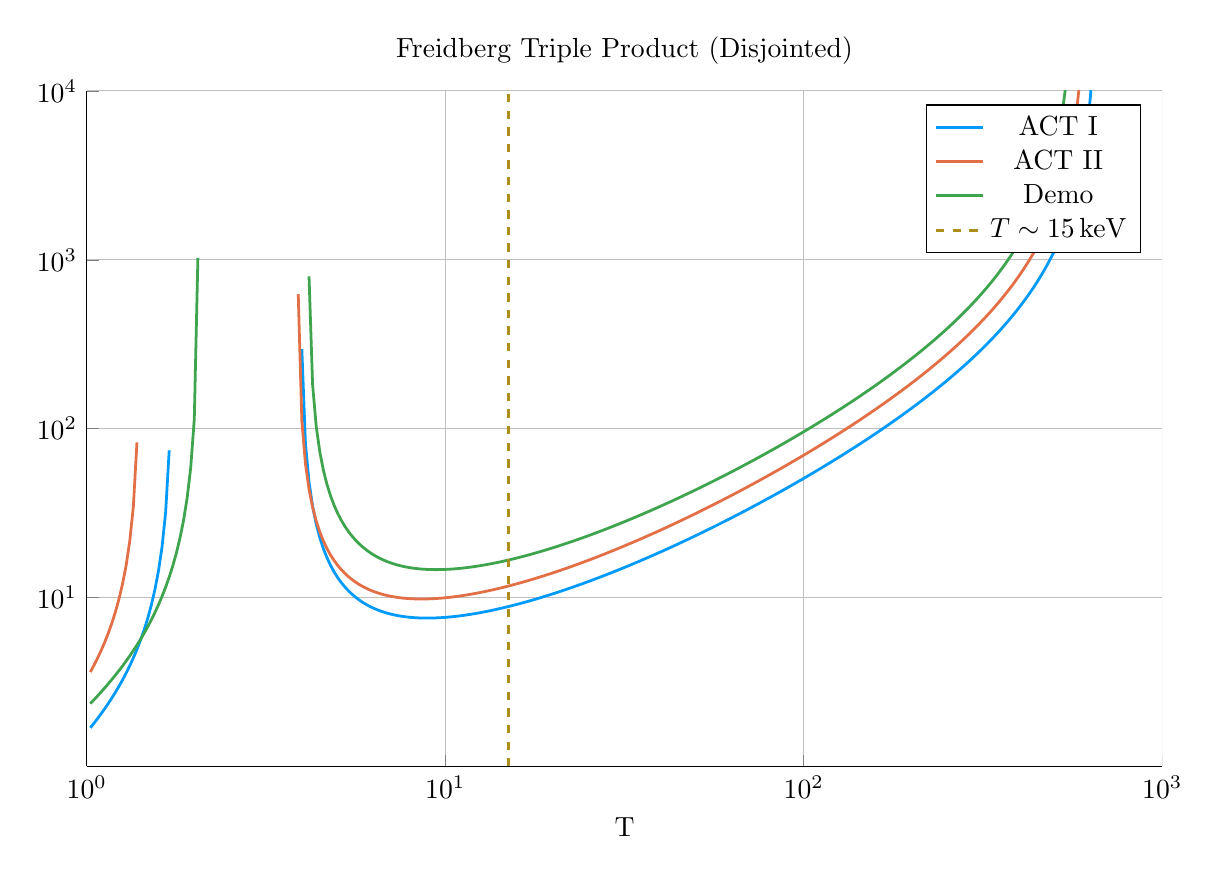
\begin{tikzpicture}[]
\begin{axis}[height = {101.6mm}, ylabel = {}, title = {Freidberg Triple Product (Disjointed)}, xmin = {1.0}, xmax = {1000.0}, ymax = {10000.0}, ymode = {log}, xlabel = {T}, {unbounded coords=jump, xticklabel style={rotate = 0}, log basis x=10, xmajorgrids = true, xtick = {1.0,10.0,100.0,1000.0}, xticklabels = {$10^{0}$,$10^{1}$,$10^{2}$,$10^{3}$}, xtick align = inside, axis lines* = left, yticklabel style={rotate = 0}, log basis y=10, ymajorgrids = true, ytick = {10.0,100.0,1000.0,10000.0}, yticklabels = {$10^{1}$,$10^{2}$,$10^{3}$,$10^{4}$}, ytick align = inside, axis lines* = left,     xshift = 0.0mm,
    yshift = 0.0mm,
    axis background/.style={fill={rgb,1:red,1.00000000;green,1.00000000;blue,1.00000000}}
}, xmode = {log}, ymin = {1.001}, width = {152.4mm}]\addplot+ [color = {rgb,1:red,0.00000000;green,0.60560316;blue,0.97868012},
draw opacity=1.0,
line width=1,
solid,mark = none,
mark size = 2.0,
mark options = {
    color = {rgb,1:red,0.00000000;green,0.00000000;blue,0.00000000}, draw opacity = 1.0,
    fill = {rgb,1:red,0.00000000;green,0.60560316;blue,0.97868012}, fill opacity = 1.0,
    line width = 1,
    rotate = 0,
    solid
}]coordinates {
(1.023292992280754, 1.6945150918881617)
(1.0471285480508996, 1.8022297212985727)
(1.0715193052376064, 1.9208400907418741)
(1.096478196143185, 2.0520379173824526)
(1.1220184543019633, 2.1978809957158)
(1.1481536214968828, 2.3608969492317664)
(1.1748975549395295, 2.5442241968703065)
(1.202264434617413, 2.7518066614453685)
(1.2302687708123816, 2.9886676965649497)
(1.2589254117941673, 3.2613035039971368)
(1.288249551693134, 3.5782615298822504)
(1.318256738556407, 3.9510138131485064)
(1.3489628825916535, 4.395316889582276)
(1.3803842646028848, 4.933406616196546)
(1.4125375446227544, 5.597693756447026)
(1.4454397707459274, 6.437310966298612)
(1.4791083881682074, 7.530455822814955)
(1.5135612484362082, 9.009551106277522)
(1.5488166189124815, 11.117997739838028)
(1.5848931924611136, 14.357045698731298)
(1.62181009735893, 19.94980446331863)
(1.6595869074375607, 31.870474474777332)
(1.6982436524617444, 74.50886497100848)
(1.7378008287493754, -268.62399052136783)
(1.7782794100389228, -49.919103932965776)
(1.8197008586099834, -28.182974323791697)
(1.8620871366628675, -19.98239680052841)
(1.9054607179632472, -15.70205772252279)
(1.9498445997580451, -13.093397062325929)
(1.9952623149688795, -11.354078520088276)
(2.041737944669529, -10.126703775296521)
(2.0892961308540396, -9.228291825900367)
(2.137962089502232, -8.555793230466092)
(2.1877616239495525, -8.047086394966504)
(2.2387211385683394, -7.662850026356773)
(2.290867652767773, -7.377360182440818)
(2.344228815319922, -7.173493942563709)
(2.3988329190194904, -7.03987823872135)
(2.4547089156850306, -6.969209177348767)
(2.51188643150958, -6.957252425128463)
(2.5703957827688635, -7.0022689551713535)
(2.6302679918953817, -7.104731798631218)
(2.6915348039269156, -7.2672686328905565)
(2.7542287033381663, -7.494810686078433)
(2.8183829312644537, -7.794966372176634)
(2.884031503126606, -8.178679918245468)
(2.9512092266663856, -8.661293939987127)
(3.019951720402016, -9.264230780294357)
(3.0902954325135905, -10.01767902164183)
(3.1622776601683795, -10.964999922356022)
(3.2359365692962827, -12.170236892008582)
(3.311311214825911, -13.7315665677587)
(3.3884415613920256, -15.806961575136446)
(3.4673685045253166, -18.667256898848134)
(3.548133892335755, -22.818098057023896)
(3.630780547701014, -29.323816090272153)
(3.715352290971725, -40.87190947609052)
(3.8018939632056115, -66.7704951710188)
(3.890451449942806, -176.00214091027135)
(3.9810717055349722, 296.2120048547568)
(4.073802778041127, 82.22608375442015)
(4.168693834703354, 48.43306336833725)
(4.265795188015927, 34.70962566295797)
(4.36515832240166, 27.295945016455207)
(4.466835921509632, 22.67019834453781)
(4.570881896148751, 19.52007287600256)
(4.677351412871983, 17.24499928723126)
(4.786300923226384, 15.531278040885976)
(4.897788193684462, 14.199095003080004)
(5.011872336272722, 13.138001469719821)
(5.1286138399136485, 12.27642393656205)
(5.248074602497725, 11.565956055783074)
(5.370317963702527, 10.972696881733755)
(5.495408738576246, 10.472204393849793)
(5.623413251903491, 10.04641840843593)
(5.7543993733715695, 9.681711040383625)
(5.88843655355589, 9.367610463946743)
(6.025595860743578, 9.095941481219963)
(6.165950018614822, 8.860232308719008)
(6.309573444801933, 8.655296117741381)
(6.456542290346556, 8.476930095683173)
(6.606934480075959, 8.321695258418004)
(6.760829753919817, 8.186752828259676)
(6.918309709189364, 8.06974093001644)
(7.079457843841379, 7.968680480243153)
(7.244359600749901, 7.881902520894599)
(7.413102413009175, 7.80799150193639)
(7.5857757502918375, 7.745740605469891)
(7.762471166286917, 7.694116194091195)
(7.943282347242816, 7.652229324407223)
(8.128305161640993, 7.619312722352829)
(8.31763771102671, 7.594702046961867)
(8.511380382023766, 7.577820541204338)
(8.709635899560805, 7.568166379774354)
(8.912509381337454, 7.565302179476453)
(9.120108393559097, 7.568846255848602)
(9.33254300796991, 7.57846529863635)
(9.549925860214358, 7.593868207120024)
(9.772372209558107, 7.614800878969009)
(10.0, 7.6410417872330525)
(10.232929922807541, 7.672398212107776)
(10.471285480508996, 7.708703019333509)
(10.715193052376065, 7.7498118970722105)
(10.964781961431852, 7.7956009790373795)
(11.220184543019636, 7.845964794420564)
(11.481536214968829, 7.9008144954472845)
(11.748975549395297, 7.960076321728849)
(12.02264434617413, 8.023690267358889)
(12.302687708123818, 8.091608922249174)
(12.589254117941675, 8.163796463753897)
(12.882495516931343, 8.240227778388245)
(13.182567385564074, 8.320887696558643)
(13.489628825916533, 8.405770325808698)
(13.803842646028846, 8.494878470244457)
(14.12537544622754, 8.588223125611163)
(14.454397707459272, 8.68582304101473)
(14.791083881682072, 8.787704339563915)
(15.13561248436208, 8.893900191356126)
(15.488166189124811, 9.00445053273945)
(15.848931924611133, 9.119401827772037)
(16.218100973589298, 9.238806866525163)
(16.595869074375607, 9.36272459734332)
(16.982436524617444, 9.49121998943775)
(17.378008287493753, 9.62436392387273)
(17.78279410038923, 9.762233108678469)
(18.197008586099834, 9.904910018476908)
(18.620871366628677, 10.052482855035347)
(19.054607179632473, 10.205045527912834)
(19.498445997580454, 10.362697653760055)
(19.952623149688797, 10.525544573138253)
(20.417379446695296, 10.693697383890798)
(20.892961308540396, 10.86727299025056)
(21.379620895022324, 11.04639416699954)
(21.87761623949553, 11.231189638117145)
(22.3872113856834, 11.42179416946176)
(22.908676527677734, 11.6183486751283)
(23.442288153199225, 11.82100033721453)
(23.9883291901949, 12.029902739089)
(24.547089156850298, 12.245216010109123)
(25.118864315095795, 12.467106987583263)
(25.703957827688633, 12.695749386290691)
(26.302679918953814, 12.931323985371597)
(26.915348039269155, 13.174018826913404)
(27.542287033381662, 13.424029428392666)
(28.183829312644534, 13.681559008968577)
(28.84031503126606, 13.946818729958853)
(29.512092266663856, 14.220027949885045)
(30.19951720402016, 14.50141449453101)
(30.902954325135905, 14.791214942515055)
(31.622776601683793, 15.089674926934103)
(32.359365692962825, 15.39704945369735)
(33.11311214825911, 15.713603237227478)
(33.884415613920254, 16.039611054270374)
(34.673685045253166, 16.375358304735574)
(35.48133892335755, 16.72114046362978)
(36.30780547701014, 17.077265375464844)
(37.15352290971726, 17.444051808101882)
(38.018939632056124, 17.821830851190978)
(38.90451449942807, 18.210946209955225)
(39.810717055349734, 18.611754712404426)
(40.73802778041128, 19.02462684323082)
(41.68693834703355, 19.44994730585631)
(42.65795188015925, 19.888115614110824)
(43.65158322401658, 20.33954671581207)
(44.6683592150963, 20.804671648648)
(45.708818961487495, 21.283938232164516)
(46.77351412871981, 21.777811796588267)
(47.86300923226383, 22.286775951266307)
(48.97788193684461, 22.811333395047512)
(50.11872336272722, 23.352006771196773)
(51.28613839913648, 23.90933956979331)
(52.48074602497726, 24.483897079598876)
(53.70317963702527, 25.07626739512277)
(54.954087385762456, 25.687062479009892)
(56.23413251903491, 26.316919285823328)
(57.543993733715695, 26.966500951119475)
(58.8843655355589, 27.63649804806381)
(60.25595860743578, 28.32762991928082)
(61.65950018614822, 29.040646086657393)
(63.09573444801933, 29.776327745458484)
(64.56542290346556, 30.535489348458338)
(66.06934480075961, 31.318980286421752)
(67.60829753919819, 32.12768667178653)
(69.18309709189366, 32.96253323296315)
(70.79457843841381, 33.82448532728458)
(72.44359600749902, 34.71455108131369)
(74.13102413009177, 35.63378366795554)
(75.85775750291836, 36.5832837306308)
(77.62471166286916, 37.56420196565578)
(79.43282347242814, 38.5777418749493)
(81.2830516164099, 39.625162702259914)
(83.17637711026708, 40.70778256728596)
(85.11380382023764, 41.82698181336084)
(87.09635899560806, 42.98420658580859)
(89.12509381337455, 44.18097265965641)
(91.20108393559097, 45.41886953713795)
(93.3254300796991, 46.69956483735465)
(95.49925860214358, 48.0248090026031)
(97.72372209558107, 49.39644034825024)
(100.0, 50.81639048567384)
(102.32929922807536, 52.28669015071427)
(104.71285480508996, 53.809475473344484)
(107.1519305237606, 55.38699472789598)
(109.64781961431851, 57.02161560723521)
(112.2018454301963, 58.71583306880927)
(114.81536214968828, 60.47227780555281)
(117.48975549395291, 62.29372540032026)
(120.22644346174131, 64.1831062288853)
(123.02687708123811, 66.14351618370313)
(125.89254117941675, 68.17822829869775)
(128.82495516931337, 70.29070536425795)
(131.82567385564073, 72.48461363302665)
(134.89628825916532, 74.76383772515437)
(138.03842646028852, 77.13249686084183)
(141.2537544622754, 79.59496255677749)
(144.5439770745928, 82.1558779437945)
(147.91083881682073, 84.82017888112068)
(151.35612484362088, 87.59311706484252)
(154.88166189124811, 90.48028535342075)
(158.48931924611142, 93.48764556200553)
(162.18100973589299, 96.62155901048361)
(165.95869074375614, 99.88882014839527)
(169.82436524617444, 103.29669362390514)
(173.78008287493762, 106.8529552149526)
(177.82794100389228, 110.56593709971621)
(181.97008586099827, 114.44457801209604)
(186.20871366628674, 118.49847890775631)
(190.54607179632464, 122.73796485951151)
(194.98445997580455, 127.17415401000369)
(199.52623149688787, 131.81903453779776)
(204.17379446695296, 136.68555074397534)
(208.92961308540387, 141.7876995445982)
(213.79620895022325, 147.14063886569335)
(218.77616239495518, 152.76080968855555)
(223.872113856834, 158.66607379276888)
(229.08676527677724, 164.87586960296383)
(234.42288153199226, 171.4113889762298)
(239.88329190194898, 178.29577828677515)
(245.4708915685031, 185.55436779375145)
(251.18864315095797, 193.21493404336246)
(257.03957827688646, 201.30800099096868)
(263.02679918953817, 209.86718667547356)
(269.1534803926917, 218.92960369175984)
(275.4228703338166, 228.5363234580894)
(281.8382931264455, 238.73291645637224)
(288.40315031266056, 249.57008335444863)
(295.1209226666387, 261.10439535985074)
(301.9951720402016, 273.39916651425244)
(309.0295432513592, 286.52548620009975)
(316.22776601683796, 300.5634472677593)
(323.5936569296281, 315.60361443723326)
(331.1311214825911, 331.74878965791873)
(338.84415613920237, 349.11614693461144)
(346.73685045253166, 367.83983008944125)
(354.8133892335753, 388.074134968045)
(363.0780547701014, 409.9974354672692)
(371.5352290971724, 433.8170644462405)
(380.1893963205613, 459.775431919879)
(389.04514499428046, 488.15776259296996)
(398.1071705534973, 519.301975844092)
(407.3802778041126, 553.6114337377378)
(416.8693834703355, 591.5715777555781)
(426.57951880159254, 633.7719123174471)
(436.5158322401661, 680.9354532594568)
(446.683592150963, 733.9587765720896)
(457.0881896148752, 793.9674013286159)
(467.73514128719813, 862.3938269620526)
(478.6300923226385, 941.0898231518593)
(489.77881936844614, 1032.4918995815904)
(501.18723362727246, 1139.8718558647272)
(512.8613839913648, 1267.728232380304)
(524.8074602497728, 1422.4206670383826)
(537.0317963702527, 1613.2432940240717)
(549.5408738576248, 1854.3379168248518)
(562.341325190349, 2168.328384373693)
(575.4399373371566, 2593.8014145005036)
(588.843655355589, 3202.400412559708)
(602.5595860743575, 4143.871725688599)
(616.5950018614822, 5792.368998792458)
(630.957344480193, 9418.65571693456)
(645.6542290346556, 23889.28171950775)
(660.6934480075957, -49140.70577934398)
(676.0829753919819, -12421.08556602776)
(691.8309709189363, -7211.5383604203)
(707.945784384138, -5131.503513512916)
(724.4359600749899, -4013.149779314024)
(741.3102413009177, -3315.290437938855)
(758.5775750291835, -2838.6775691444445)
(776.247116628692, -2492.7815835486012)
(794.3282347242813, -2230.5404344031062)
(812.8305161640995, -2025.0671265994276)
(831.7637711026708, -1859.8852065397507)
(851.1380382023768, -1724.3348515292655)
(870.9635899560806, -1611.214292586841)
(891.2509381337459, -1515.482798133364)
(912.0108393559096, -1433.5066904171208)
(933.2543007969915, -1362.60044755666)
(954.992586021436, -1300.7364064371823)
(977.2372209558112, -1246.3549673169614)
(1000.0, -1198.236922422159)
(1023.2929922807537, -1155.4154111586524)
(1047.1285480508996, -1117.1138595692732)
(1071.519305237606, -1082.7013755947412)
(1096.4781961431852, -1051.6601296512954)
(1122.018454301963, -1023.5611236164838)
(1148.1536214968828, -998.0459352192751)
(1174.897554939529, -974.8127865165062)
(1202.2644346174131, -953.6057869052796)
(1230.268770812381, -934.2065376059747)
(1258.9254117941675, -916.427514142416)
(1288.2495516931335, -900.1068024887031)
(1318.2567385564075, -885.1038764728944)
(1348.9628825916532, -871.2961837984906)
(1380.3842646028852, -858.5763656093441)
(1412.537544622754, -846.8499765447623)
(1445.439770745928, -836.0336032365552)
(1479.1083881682073, -826.0533023067777)
(1513.5612484362086, -816.8432963076928)
(1548.816618912481, -808.3448792375339)
(1584.893192461114, -800.5054933601936)
(1621.8100973589299, -793.2779468416144)
(1659.5869074375614, -786.619747763086)
(1698.2436524617442, -780.4925348022881)
(1737.8008287493763, -774.8615885976767)
(1778.2794100389228, -769.695410762998)
(1819.7008586099826, -764.9653598706944)
(1862.0871366628676, -760.6453356042871)
(1905.4607179632462, -756.7115038241651)
(1949.8445997580454, -753.1420564513764)
(1995.2623149688789, -749.9170011631115)
(2041.7379446695295, -747.017976692142)
(2089.296130854039, -744.4280901019075)
(2137.9620895022326, -742.1317730997671)
(2187.761623949552, -740.1146548191589)
(2238.72113856834, -738.3634489135239)
(2290.8676527677726, -736.8658531085748)
(2344.228815319923, -735.6104596965912)
(2398.83291901949, -734.5866754712753)
(2454.708915685031, -733.7846501343085)
(2511.88643150958, -733.1952120249796)
(2570.3957827688646, -732.8098103606878)
(2630.2679918953813, -732.6204632251878)
(2691.5348039269165, -732.619710649065)
(2754.2287033381663, -732.8005722110505)
(2818.382931264455, -733.1565086609373)
(2884.031503126606, -733.6813871269079)
(2951.209226666387, -734.3694495236135)
(3019.9517204020162, -735.2152838235631)
(3090.295432513592, -736.2137978944917)
(3162.2776601683795, -737.3601956401093)
(3235.936569296281, -738.6499552119711)
(3311.311214825911, -740.0788090865385)
(3388.441561392024, -741.6427258246325)
(3467.368504525317, -743.3378933506358)
(3548.133892335753, -745.1607036065371)
(3630.780547701014, -747.1077384514889)
(3715.352290971724, -749.1757566912511)
(3801.8939632056126, -751.3616821340012)
(3890.4514499428046, -753.6625925796814)
(3981.0717055349733, -756.0757096595084)
(4073.802778041126, -758.5983894506668)
(4168.693834703355, -761.2281137986595)
(4265.795188015925, -763.9624822864063)
(4365.158322401661, -766.7992045807192)
(4466.835921509631, -769.7360946070586)
(4570.881896148751, -772.7710620056145)
(4677.351412871981, -775.9021083311076)
(4786.300923226385, -779.1273204560445)
(4897.7881936844615, -782.4448656456962)
(5011.872336272725, -785.8529867735253)
(5128.613839913648, -789.3499978635558)
(5248.074602497728, -792.9342799342446)
(5370.317963702527, -796.604277116354)
(5495.408738576249, -800.3584930490041)
(5623.413251903491, -804.195487472099)
(5754.399373371566, -808.1138730792338)
(5888.43655355589, -812.1123125544108)
(6025.595860743575, -816.1895158014244)
(6165.9500186148225, -820.3442373483241)
(6309.57344480193, -824.575273914367)
(6456.542290346556, -828.8814621278906)
(6606.934480075957, -833.2616763844619)
(6760.829753919818, -837.7148268354883)
(6918.309709189362, -842.2398574982564)
(7079.457843841381, -846.8357444790493)
(7244.359600749898, -851.5014943016532)
(7413.102413009177, -856.2361423341288)
(7585.775750291836, -861.0387513072818)
(7762.4711662869195, -865.9084099187404)
(7943.282347242814, -870.8442315170112)
(8128.305161640995, -875.8453528602984)
(8317.63771102671, -880.9109329452398)
(8511.380382023768, -886.0401519010943)
(8709.635899560806, -891.2322099451943)
(8912.509381337459, -896.4863263958177)
(9120.108393559096, -901.8017387388758)
(9332.543007969914, -907.1777017450888)
(9549.92586021436, -912.6134865547074)
(9772.372209558112, -918.1083801920363)
(10000.0, -923.6616844862497)
};
\addlegendentry{ACT I}
\addplot+ [color = {rgb,1:red,0.88887350;green,0.43564919;blue,0.27812294},
draw opacity=1.0,
line width=1,
solid,mark = none,
mark size = 2.0,
mark options = {
    color = {rgb,1:red,0.00000000;green,0.00000000;blue,0.00000000}, draw opacity = 1.0,
    fill = {rgb,1:red,0.88887350;green,0.43564919;blue,0.27812294}, fill opacity = 1.0,
    line width = 1,
    rotate = 0,
    solid
}]coordinates {
(1.023292992280754, 3.6262198595749764)
(1.0471285480508996, 3.9709951177889846)
(1.0715193052376064, 4.3756174014389835)
(1.096478196143185, 4.856923072933348)
(1.1220184543019633, 5.438683072221177)
(1.1481536214968828, 6.155573870975628)
(1.1748975549395295, 7.060228008162098)
(1.202264434617413, 8.236563724204407)
(1.2302687708123816, 9.827054231195484)
(1.2589254117941673, 12.094532497587037)
(1.288249551693134, 15.583209353705142)
(1.318256738556407, 21.63257843385939)
(1.3489628825916535, 34.66570824747554)
(1.3803842646028848, 83.08790958003418)
(1.4125375446227544, -237.94957827646257)
(1.4454397707459274, -50.355280711590225)
(1.4791083881682074, -28.63496801892399)
(1.5135612484362082, -20.251666213285585)
(1.5488166189124815, -15.820177297479631)
(1.5848931924611136, -13.08951908492532)
(1.62181009735893, -11.24674808778935)
(1.6595869074375607, -9.926910662341783)
(1.6982436524617444, -8.941965953571943)
(1.7378008287493754, -8.185314268502955)
(1.7782794100389228, -7.592149139482488)
(1.8197008586099834, -7.120936958963385)
(1.8620871366628675, -6.74396430844709)
(1.9054607179632472, -6.442168044456181)
(1.9498445997580451, -6.202147460832283)
(1.9952623149688795, -6.014359309768401)
(2.041737944669529, -5.871988456076733)
(2.0892961308540396, -5.770222564971642)
(2.137962089502232, -5.705778915745288)
(2.1877616239495525, -5.676595450141278)
(2.2387211385683394, -5.68163408082953)
(2.290867652767773, -5.720765456471678)
(2.344228815319922, -5.794717627708497)
(2.3988329190194904, -5.9050800796980125)
(2.4547089156850306, -6.054361567255678)
(2.51188643150958, -6.246106580679075)
(2.5703957827688635, -6.485082333271136)
(2.6302679918953817, -6.777557290905968)
(2.6915348039269156, -7.1317054161224025)
(2.7542287033381663, -7.558190626573394)
(2.8183829312644537, -8.071018969252556)
(2.884031503126606, -8.688801804272321)
(2.9512092266663856, -9.436671353402025)
(3.019951720402016, -10.349269580424053)
(3.0902954325135905, -11.475575910838932)
(3.1622776601683795, -12.887036452859418)
(3.2359365692962827, -14.691959839828085)
(3.311311214825911, -17.06263857450721)
(3.3884415613920256, -20.29057894681975)
(3.4673685045253166, -24.910913722214016)
(3.548133892335755, -32.02376727816436)
(3.630780547701014, -44.30667919768318)
(3.715352290971725, -70.4202182892387)
(3.8018939632056115, -162.8647166076088)
(3.890451449942806, 626.9103884763274)
(3.9810717055349722, 111.1855857788192)
(4.073802778041127, 62.30641416623654)
(4.168693834703354, 43.93800066040291)
(4.265795188015927, 34.33706014393487)
(4.36515832240166, 28.454603024787982)
(4.466835921509632, 24.493996588522855)
(4.570881896148751, 21.655444964297164)
(4.677351412871983, 19.528883534080794)
(4.786300923226384, 17.882391475312325)
(4.897788193684462, 16.574948455957568)
(5.011872336272722, 15.51588818674524)
(5.1286138399136485, 14.644277005698534)
(5.248074602497725, 13.917659005030185)
(5.370317963702527, 13.305553561598769)
(5.495408738576246, 12.785518065105022)
(5.623413251903491, 12.340668088629867)
(5.7543993733715695, 11.958062188819154)
(5.88843655355589, 11.627618960477479)
(6.025595860743578, 11.341372389870859)
(6.165950018614822, 11.092948328333481)
(6.309573444801933, 10.877189105947096)
(6.456542290346556, 10.689879592932128)
(6.606934480075959, 10.527544110660646)
(6.760829753919817, 10.387293705403508)
(6.918309709189364, 10.266709799369176)
(7.079457843841379, 10.16375450253595)
(7.244359600749901, 10.076700725700801)
(7.413102413009175, 10.004077180609906)
(7.5857757502918375, 9.944624699045534)
(7.762471166286917, 9.897261247744884)
(7.943282347242816, 9.861053688507223)
(8.128305161640993, 9.835194817415095)
(8.31763771102671, 9.818984570337387)
(8.511380382023766, 9.811814542185662)
(8.709635899560805, 9.813155162447515)
(8.912509381337454, 9.822545006156611)
(9.120108393559097, 9.83958185650335)
(9.33254300796991, 9.863915174108707)
(9.549925860214358, 9.895239747025146)
(9.772372209558107, 9.933290289132369)
(10.0, 9.977836853773296)
(10.232929922807541, 10.028680908432321)
(10.471285480508996, 10.085651971057402)
(10.715193052376065, 10.148604718433416)
(10.964781961431852, 10.21741649362127)
(11.220184543019636, 10.291985152574611)
(11.481536214968829, 10.37222719997026)
(11.748975549395297, 10.458076172688434)
(12.02264434617413, 10.549481236152369)
(12.302687708123818, 10.64640596430817)
(12.589254117941675, 10.748827278619041)
(12.882495516931343, 10.856734525250282)
(13.182567385564074, 10.970128672782435)
(13.489628825916533, 11.089021615426763)
(13.803842646028846, 11.213435568926192)
(14.12537544622754, 11.343402548181452)
(14.454397707459272, 11.478963917208173)
(14.791083881682072, 11.620170003356527)
(15.13561248436208, 11.767079768850763)
(15.488166189124811, 11.919760533665668)
(15.848931924611133, 12.078287744603548)
(16.218100973589298, 12.242744785962834)
(16.595869074375607, 12.413222828300148)
(16.982436524617444, 12.589820711506782)
(17.378008287493753, 12.772644859640952)
(17.78279410038923, 12.961809224911852)
(18.197008586099834, 13.157435258695006)
(18.620871366628677, 13.359651907740494)
(19.054607179632473, 13.568595633881658)
(19.498445997580454, 13.78441045660099)
(19.952623149688797, 14.007248015617566)
(20.417379446695296, 14.237267654769363)
(20.892961308540396, 14.474636524779191)
(21.379620895022324, 14.719529704908814)
(21.87761623949553, 14.972130342899538)
(22.3872113856834, 15.232629812825081)
(22.908676527677734, 15.501227890845222)
(23.442288153199225, 15.778132947219865)
(23.9883291901949, 16.06356215819839)
(24.547089156850298, 16.35774173268541)
(25.118864315095795, 16.660907159108888)
(25.703957827688633, 16.973303467018464)
(26.302679918953814, 17.295185509573656)
(26.915348039269155, 17.62681826308181)
(27.542287033381662, 17.96847714569595)
(28.183829312644534, 18.32044835551375)
(28.84031503126606, 18.6830292286709)
(29.512092266663856, 19.05652861809976)
(30.19951720402016, 19.441267293702094)
(30.902954325135905, 19.837578364764788)
(31.622776601683793, 20.245807725529637)
(32.359365692962825, 20.66631452491334)
(33.11311214825911, 21.099471661462132)
(33.884415613920254, 21.54566630471813)
(34.673685045253166, 22.00530044427105)
(35.48133892335755, 22.47879146787113)
(36.30780547701014, 22.966572770086653)
(37.15352290971726, 23.469094393103948)
(38.018939632056124, 23.986823701388534)
(38.90451449942807, 24.520246092055554)
(39.810717055349734, 25.069865742935068)
(40.73802778041128, 25.636206400465333)
(41.68693834703355, 26.219812206925383)
(42.65795188015925, 26.82124858892035)
(43.65158322401658, 27.441103151399624)
(44.6683592150963, 28.079986677312778)
(45.708818961487495, 28.73853413868146)
(46.77351412871981, 29.417405780721598)
(47.86300923226383, 30.117288263079946)
(48.97788193684461, 30.838895864745762)
(50.11872336272722, 31.582971756705206)
(51.28613839913648, 32.35028934671438)
(52.48074602497726, 33.14165370090234)
(53.70317963702527, 33.957903047277725)
(54.954087385762456, 34.79991036660676)
(56.23413251903491, 35.668585076557704)
(57.543993733715695, 36.56487481530732)
(58.8843655355589, 37.4897673324607)
(60.25595860743578, 38.44429249224886)
(61.65950018614822, 39.42952440027207)
(63.09573444801933, 40.44658366003865)
(64.56542290346556, 41.496639769647544)
(66.06934480075961, 42.58091366862388)
(67.60829753919819, 43.70068044592992)
(69.18309709189366, 44.857272221109575)
(70.79457843841381, 46.052081211550274)
(72.44359600749902, 47.286562999969696)
(74.13102413009177, 48.562240017471)
(75.85775750291836, 49.8807052588659)
(77.62471166286916, 51.243626248459464)
(79.43282347242814, 52.65274927613318)
(81.2830516164099, 54.10990392537751)
(83.17637711026708, 55.617007916924386)
(85.11380382023764, 57.17607229384146)
(87.09635899560806, 58.78920697639489)
(89.12509381337455, 60.458626717694976)
(91.20108393559097, 62.18665749414143)
(93.3254300796991, 63.97574336801635)
(95.49925860214358, 65.82845386036456)
(97.72372209558107, 67.74749189972668)
(100.0, 69.73570233531223)
(102.32929922807536, 71.79608117146411)
(104.71285480508996, 73.93178548206338)
(107.1519305237606, 76.14614413306579)
(109.64781961431851, 78.44266936696852)
(112.2018454301963, 80.8250693343548)
(114.81536214968828, 83.29726166380183)
(117.48975549395291, 85.86338817160895)
(120.22644346174131, 88.52783082428154)
(123.02687708123811, 91.29522907965378)
(125.89254117941675, 94.17049874718609)
(128.82495516931337, 97.15885252455993)
(131.82567385564073, 100.26582238652995)
(134.89628825916532, 103.497284023392)
(138.03842646028852, 106.8594835506073)
(141.2537544622754, 110.35906674040386)
(144.5439770745928, 114.00311105358536)
(147.91083881682073, 117.79916079358593)
(151.35612484362088, 121.75526573929804)
(154.88166189124811, 125.88002366576029)
(158.48931924611142, 130.1826272158626)
(162.18100973589299, 134.672915650604)
(165.95869074375614, 139.36143207981326)
(169.82436524617444, 144.25948686159074)
(173.78008287493762, 149.37922795930874)
(177.82794100389228, 154.73371916238966)
(181.97008586099827, 160.33702721452812)
(186.20871366628674, 166.20431905434293)
(190.54607179632464, 172.35197056339555)
(194.98445997580455, 178.79768844082054)
(199.52623149688787, 185.56064708952624)
(204.17379446695296, 192.66164271474446)
(208.92961308540387, 200.12326721230153)
(213.79620895022325, 207.97010486869286)
(218.77616239495518, 216.2289554844475)
(223.872113856834, 224.92908801677567)
(229.08676527677724, 234.10252996410594)
(234.42288153199226, 243.78439825504503)
(239.88329190194898, 254.013278913416)
(245.4708915685031, 264.831664041007)
(251.18864315095797, 276.2864564799751)
(257.03957827688646, 288.42955470570877)
(263.02679918953817, 301.31853323333485)
(269.1534803926917, 315.01743724146417)
(275.4228703338166, 329.5977144230688)
(281.8382931264455, 345.13931252826)
(288.40315031266056, 361.7319780177609)
(295.1209226666387, 379.47680017147866)
(301.9951720402016, 398.48805653482157)
(309.0295432513592, 418.8954306148157)
(316.22776601683796, 440.8466924729332)
(323.5936569296281, 464.5109589979699)
(331.1311214825911, 490.0826855730525)
(338.84415613920237, 517.7865879974996)
(346.73685045253166, 547.8837577991267)
(354.8133892335753, 580.6793227491402)
(363.0780547701014, 616.5321281016747)
(371.5352290971724, 655.8670890363044)
(380.1893963205613, 699.1911156139116)
(389.04514499428046, 747.1138767235202)
(398.1071705534973, 800.3752099841976)
(407.3802778041126, 859.8817991675508)
(416.8693834703355, 926.7569931156614)
(426.57951880159254, 1002.409608394075)
(436.5158322401661, 1088.6307275063882)
(446.683592150963, 1187.7327493644536)
(457.0881896148752, 1302.7538970715893)
(467.73514128719813, 1437.7671929229414)
(478.6300923226385, 1598.3619531251416)
(489.77881936844614, 1792.4217156957561)
(501.18723362727246, 2031.435864125701)
(512.8613839913648, 2332.8272604727294)
(524.8074602497728, 2724.3501891507594)
(537.0317963702527, 3253.0808589923313)
(549.5408738576248, 4005.7745115556468)
(562.341325190349, 5161.830905458572)
(575.4399373371566, 7161.999955047848)
(588.843655355589, 11456.916643900393)
(602.5595860743575, 27278.085748054084)
(616.5950018614822, -81374.99567859212)
(630.957344480193, -16777.758330681536)
(645.6542290346556, -9494.611990167594)
(660.6934480075957, -6689.456467425088)
(676.0829753919819, -5204.544925417548)
(691.8309709189363, -4286.084695387924)
(707.945784384138, -3662.3824611701343)
(724.4359600749899, -3211.5569830118793)
(741.3102413009177, -2870.7907078330154)
(758.5775750291835, -2604.4181322887152)
(776.247116628692, -2390.6863963037536)
(794.3282347242813, -2215.5742233715514)
(812.8305161640995, -2069.6372672190055)
(831.7637711026708, -1946.2815219657975)
(851.1380382023768, -1840.7635003469652)
(870.9635899560806, -1749.5836745614658)
(891.2509381337459, -1670.1038187095141)
(912.0108393559096, -1600.2974165784447)
(933.2543007969915, -1538.5821079233035)
(954.992586021436, -1483.704347654581)
(977.2372209558112, -1434.6582328197553)
(1000.0, -1390.6272443725638)
(1023.2929922807537, -1350.9416958920935)
(1047.1285480508996, -1315.0471613093978)
(1071.519305237606, -1282.4807127947604)
(1096.4781961431852, -1252.8528041238237)
(1122.018454301963, -1225.8332942321483)
(1148.1536214968828, -1201.1405477147484)
(1174.897554939529, -1178.5328496873165)
(1202.2644346174131, -1157.8015815679175)
(1230.268770812381, -1138.765750110663)
(1258.9254117941675, -1121.267566697522)
(1288.2495516931335, -1105.1688489426283)
(1318.2567385564075, -1090.348071514546)
(1348.9628825916532, -1076.6979335079102)
(1380.3842646028852, -1064.1233398013928)
(1412.537544622754, -1052.539716470997)
(1445.439770745928, -1041.8715974920947)
(1479.1083881682073, -1032.0514330898977)
(1513.5612484362086, -1023.018580214714)
(1548.816618912481, -1014.7184434731793)
(1584.893192461114, -1007.1017409878611)
(1621.8100973589299, -1000.1238744907862)
(1659.5869074375614, -993.744386783934)
(1698.2436524617442, -987.9264927488415)
(1737.8008287493763, -982.636672530169)
(1778.2794100389228, -977.8443174854673)
(1819.7008586099826, -973.5214210860804)
(1862.0871366628676, -969.6423082497454)
(1905.4607179632462, -966.1833976443339)
(1949.8445997580454, -963.1229923714116)
(1995.2623149688789, -960.4410951549132)
(2041.7379446695295, -958.1192447533882)
(2089.296130854039, -956.1403708072178)
(2137.9620895022326, -954.4886644127564)
(2187.761623949552, -953.1494647041984)
(2238.72113856834, -952.1091527568241)
(2290.8676527677726, -951.3550628814313)
(2344.228815319923, -950.8753984451814)
(2398.83291901949, -950.6591580412987)
(2454.708915685031, -950.6960687224226)
(2511.88643150958, -950.976525783883)
(2570.3957827688646, -951.4915383610024)
(2630.2679918953813, -952.2326801933348)
(2691.5348039269165, -953.1920450178479)
(2754.2287033381663, -954.3622060364678)
(2818.382931264455, -955.7361791027337)
(2884.031503126606, -957.3073891869254)
(2951.209226666387, -959.0696398044653)
(3019.9517204020162, -961.0170851050241)
(3090.295432513592, -963.1442043574473)
(3162.2776601683795, -965.4457785953113)
(3235.936569296281, -967.9168692139419)
(3311.311214825911, -970.5527983325226)
(3388.441561392024, -973.3491307549663)
(3467.368504525317, -976.301657380888)
(3548.133892335753, -979.406379933558)
(3630.780547701014, -982.6594968855042)
(3715.352290971724, -986.0573904745661)
(3801.8939632056126, -989.5966147140405)
(3890.4514499428046, -993.2738843101055)
(3981.0717055349733, -997.0860644082568)
(4073.802778041126, -1001.030161098068)
(4168.693834703355, -1005.1033126123773)
(4265.795188015925, -1009.3027811630325)
(4365.158322401661, -1013.6259453607602)
(4466.835921509631, -1018.0702931715625)
(4570.881896148751, -1022.633415366397)
(4677.351412871981, -1027.3129994248159)
(4786.300923226385, -1032.1068237614704)
(4897.7881936844615, -1037.0127529096899)
(5011.872336272725, -1042.0287316317933)
(5128.613839913648, -1047.1527812631514)
(5248.074602497728, -1052.3829949308802)
(5370.317963702527, -1057.7175336249259)
(5495.408738576249, -1063.1546224338358)
(5623.413251903491, -1068.6925470213334)
(5754.399373371566, -1074.3296503261488)
(5888.43655355589, -1080.0643294689673)
(6025.595860743575, -1085.8950328516705)
(6165.9500186148225, -1091.8202574352306)
(6309.57344480193, -1097.8385461836895)
(6456.542290346556, -1103.9484856626516)
(6606.934480075957, -1110.1487037816134)
(6760.829753919818, -1116.437867667452)
(6918.309709189362, -1122.8146816767116)
(7079.457843841381, -1129.2778854970907)
(7244.359600749898, -1135.8262523843705)
(7413.102413009177, -1142.4585874877714)
(7585.775750291836, -1149.1737262727324)
(7762.4711662869195, -1155.9705330323777)
(7943.282347242814, -1162.847899481954)
(8128.305161640995, -1169.8047434309324)
(8317.63771102671, -1176.840007527851)
(8511.380382023768, -1183.9526580733384)
(8709.635899560806, -1191.141683897054)
(8912.509381337459, -1198.4060952946172)
(9120.108393559096, -1205.7449230208424)
(9332.543007969914, -1213.1572173358775)
(9549.92586021436, -1220.642047101055)
(9772.372209558112, -1228.198498921507)
(10000.0, -1235.8256763101228)
};
\addlegendentry{ACT II}
\addplot+ [color = {rgb,1:red,0.24222430;green,0.64327509;blue,0.30444865},
draw opacity=1.0,
line width=1,
solid,mark = none,
mark size = 2.0,
mark options = {
    color = {rgb,1:red,0.00000000;green,0.00000000;blue,0.00000000}, draw opacity = 1.0,
    fill = {rgb,1:red,0.24222430;green,0.64327509;blue,0.30444865}, fill opacity = 1.0,
    line width = 1,
    rotate = 0,
    solid
}]coordinates {
(1.023292992280754, 2.35717971253544)
(1.0471285480508996, 2.4818091803011884)
(1.0715193052376064, 2.6160533994079267)
(1.096478196143185, 2.7610169738489345)
(1.1220184543019633, 2.9179792560669826)
(1.1481536214968828, 3.088429876891961)
(1.1748975549395295, 3.2741132141278877)
(1.202264434617413, 3.4770845203202887)
(1.2302687708123816, 3.6997814161989337)
(1.2589254117941673, 3.9451158626625746)
(1.288249551693134, 4.216593759892962)
(1.318256738556407, 4.5184723163672)
(1.3489628825916535, 4.8559698120095405)
(1.3803842646028848, 5.235549216958988)
(1.4125375446227544, 5.6653077812466694)
(1.4454397707459274, 6.155521704098852)
(1.4791083881682074, 6.719422812007362)
(1.5135612484362082, 7.374331069416676)
(1.5488166189124815, 8.143348442005678)
(1.5848931924611136, 9.0579674025362)
(1.62181009735893, 10.162226448053275)
(1.6595869074375607, 11.51959922678817)
(1.6982436524617444, 13.224971744537322)
(1.7378008287493754, 15.426704428972686)
(1.7782794100389228, 18.37029833004982)
(1.8197008586099834, 22.493152913401733)
(1.8620871366628675, 28.65703826424774)
(1.9054607179632472, 38.826389394454985)
(1.9498445997580451, 58.65838956889421)
(1.9952623149688795, 113.86026736745272)
(2.041737944669529, 1028.465896265156)
(2.0892961308540396, -156.98955302050203)
(2.137962089502232, -75.58944517456705)
(2.1877616239495525, -51.04391619634808)
(2.2387211385683394, -39.30966054980392)
(2.290867652767773, -32.5119531577225)
(2.344228815319922, -28.143264194500333)
(2.3988329190194904, -25.158071654062468)
(2.4547089156850306, -23.0445846464956)
(2.51188643150958, -21.52440818514324)
(2.5703957827688635, -20.43488629677609)
(2.6302679918953817, -19.676536809340007)
(2.6915348039269156, -19.18724883626914)
(2.7542287033381663, -18.92875930297599)
(2.8183829312644537, -18.87930979578657)
(2.884031503126606, -19.02971234594769)
(2.9512092266663856, -19.381519932557275)
(3.019951720402016, -19.946725352708658)
(3.0902954325135905, -20.74884656063491)
(3.1622776601683795, -21.825612263340254)
(3.2359365692962827, -23.233892020991846)
(3.311311214825911, -25.05821583556076)
(3.3884415613920256, -27.425575246468597)
(3.4673685045253166, -30.532068258328167)
(3.548133892335755, -34.6936386598954)
(3.630780547701014, -40.450370735740485)
(3.715352290971725, -48.803893211628264)
(3.8018939632056115, -61.839107568518806)
(3.890451449942806, -84.72360389451674)
(3.9810717055349722, -134.73071514219606)
(4.073802778041127, -326.7218117310164)
(4.168693834703354, 798.2884776786321)
(4.265795188015927, 182.0559821932355)
(4.36515832240166, 103.75476422947621)
(4.466835921509632, 73.15084324411494)
(4.570881896148751, 56.90014770917698)
(4.677351412871983, 46.86280231089802)
(4.786300923226384, 40.07409117664327)
(4.897788193684462, 35.19587156238823)
(5.011872336272722, 31.53573209180628)
(5.1286138399136485, 28.69950502793406)
(5.248074602497725, 26.446359733467812)
(5.370317963702527, 24.620894487256926)
(5.495408738576246, 23.11837741508691)
(5.623413251903491, 21.86567883944471)
(5.7543993733715695, 20.81020944532067)
(5.88843655355589, 19.91319942113111)
(6.025595860743578, 19.145453338573617)
(6.165950018614822, 18.484578493662337)
(6.309573444801933, 17.91312275369926)
(6.456542290346556, 17.417291943801875)
(6.606934480075959, 16.98604667476511)
(6.760829753919817, 16.610453971230086)
(6.918309709189364, 16.283213587869994)
(7.079457843841379, 15.998306518944684)
(7.244359600749901, 15.750730470203408)
(7.413102413009175, 15.536298211082281)
(7.5857757502918375, 15.351482055139172)
(7.762471166286917, 15.193292627587141)
(7.943282347242816, 15.059183429252593)
(8.128305161640993, 14.946975025647662)
(8.31763771102671, 14.854794320700986)
(8.511380382023766, 14.781025536184384)
(8.709635899560805, 14.7242703555862)
(8.912509381337454, 14.683315302358887)
(9.120108393559097, 14.65710487318027)
(9.33254300796991, 14.644719282590849)
(9.549925860214358, 14.645355927794705)
(9.772372209558107, 14.658313873881836)
(10.0, 14.682980806167361)
(10.232929922807541, 14.718822009214483)
(10.471285480508996, 14.765371019745997)
(10.715193052376065, 14.822221669168664)
(10.964781961431852, 14.889021285358137)
(11.220184543019636, 14.965464866053368)
(11.481536214968829, 15.05129007022395)
(11.748975549395297, 15.14627290102121)
(12.02264434617413, 15.25022397586703)
(12.302687708123818, 15.362985297092992)
(12.589254117941675, 15.484427450328177)
(12.882495516931343, 15.614447171583684)
(13.182567385564074, 15.752965230502607)
(13.489628825916533, 15.899924588336324)
(13.803842646028846, 16.055288793998695)
(14.12537544622754, 16.219040587639775)
(14.454397707459272, 16.391180685479707)
(14.791083881682072, 16.571726724885952)
(15.13561248436208, 16.760712347737194)
(15.488166189124811, 16.95818640970398)
(15.848931924611133, 17.164212298589476)
(16.218100973589298, 17.378867350854325)
(16.595869074375607, 17.60224235578842)
(16.982436524617444, 17.834441138402067)
(17.378008287493753, 18.075580213329598)
(17.78279410038923, 18.325788503087594)
(18.197008586099834, 18.58520711493611)
(18.620871366628677, 18.85398917137603)
(19.054607179632473, 19.132299689997243)
(19.498445997580454, 19.420315508987848)
(19.952623149688797, 19.718225255134794)
(20.417379446695296, 20.026229351605068)
(20.892961308540396, 20.344540063200334)
(21.379620895022324, 20.673381577137132)
(21.87761623949553, 21.012990117724218)
(22.3872113856834, 21.36361409359547)
(22.908676527677734, 21.725514276034158)
(23.442288153199225, 22.09896400968359)
(23.9883291901949, 22.48424945066888)
(24.547089156850298, 22.881669834048008)
(25.118864315095795, 23.29153777529909)
(25.703957827688633, 23.714179595465023)
(26.302679918953814, 24.1499356783425)
(26.915348039269155, 24.599160856667968)
(27.542287033381662, 25.062224828200716)
(28.183829312644534, 25.539512602223876)
(28.84031503126606, 26.031424977123194)
(29.512092266663856, 26.53837904984218)
(30.19951720402016, 27.060808758149086)
(30.902954325135905, 27.599165456789784)
(31.622776601683793, 28.153918528740398)
(32.359365692962825, 28.725556028091596)
(33.11311214825911, 29.314585389840012)
(33.884415613920254, 29.92153410692588)
(34.673685045253166, 30.54695054518941)
(35.48133892335755, 31.191404729363835)
(36.30780547701014, 31.85548920357142)
(37.15352290971726, 32.539819934883965)
(38.018939632056124, 33.2450372671933)
(38.90451449942807, 33.97180692875365)
(39.810717055349734, 34.720821094770145)
(40.73802778041128, 35.49279951031094)
(41.68693834703355, 36.28849067540826)
(42.65795188015925, 37.10867309667045)
(43.65158322401658, 37.95415660928692)
(44.6683592150963, 38.82578377371943)
(45.708818961487495, 39.724431351691656)
(46.77351412871981, 40.65101186650543)
(47.86300923226383, 41.606475253047016)
(48.97788193684461, 42.59181060316595)
(50.11872336272722, 43.6080480128369)
(51.28613839913648, 44.65626053774646)
(52.48074602497726, 45.73756626505624)
(53.70317963702527, 46.8531305065716)
(54.954087385762456, 48.00416812806276)
(56.23413251903491, 49.191946015931904)
(57.543993733715695, 50.41778569686905)
(58.8843655355589, 51.68306611904523)
(60.25595860743578, 52.989226606822776)
(61.65950018614822, 54.33777000158897)
(63.09573444801933, 55.730266002386294)
(64.56542290346556, 57.16835472118021)
(66.06934480075961, 58.6537504688871)
(67.60829753919819, 60.188245789690065)
(69.18309709189366, 61.77371576271342)
(70.79457843841381, 63.41212259182487)
(72.44359600749902, 65.10552050177131)
(74.13102413009177, 66.85606099634911)
(75.85775750291836, 68.66599841255625)
(77.62471166286916, 70.53769595522424)
(79.43282347242814, 72.47363208934415)
(81.2830516164099, 74.47640741841091)
(83.17637711026708, 76.54875205648534)
(85.11380382023764, 78.69353354087694)
(87.09635899560806, 80.91376533210672)
(89.12509381337455, 83.21261595246393)
(91.20108393559097, 85.59341881965305)
(93.3254300796991, 88.05968283780572)
(95.49925860214358, 90.61510381458238)
(97.72372209558107, 93.26357678029993)
(100.0, 96.00920929309494)
(102.32929922807536, 98.85633582318225)
(104.71285480508996, 101.80953331943044)
(107.1519305237606, 104.87363807290143)
(109.64781961431851, 108.05376400487297)
(112.2018454301963, 111.35532252137295)
(114.81536214968828, 114.78404409266237)
(117.48975549395291, 118.34600173553473)
(120.22644346174131, 122.04763659144128)
(123.02687708123811, 125.89578583443561)
(125.89254117941675, 129.89771314265255)
(128.82495516931337, 134.06114202456072)
(131.82567385564073, 138.39429231126618)
(134.89628825916532, 142.9059201716157)
(138.03842646028852, 147.60536205264688)
(141.2537544622754, 152.50258300133495)
(144.5439770745928, 157.60822988511444)
(147.91083881682073, 162.93369009965753)
(151.35612484362088, 168.4911564345786)
(154.88166189124811, 174.29369885598337)
(158.48931924611142, 180.35534412396194)
(162.18100973589299, 186.6911641591149)
(165.95869074375614, 193.31737439360472)
(169.82436524617444, 200.25144347424498)
(173.78008287493762, 207.5122157275964)
(177.82794100389228, 215.12004829313008)
(181.97008586099827, 223.09696495296473)
(186.20871366628674, 231.46682908778078)
(190.54607179632464, 240.2555385901752)
(194.98445997580455, 249.49124605601838)
(199.52623149688787, 259.2046081609023)
(204.17379446695296, 269.42906883450684)
(208.92961308540387, 280.2011816981363)
(213.79620895022325, 291.56097826457074)
(218.77616239495518, 303.5523896585691)
(223.872113856834, 316.22373115690675)
(229.08676527677724, 329.6282607402076)
(234.42288153199226, 343.8248251873222)
(239.88329190194898, 358.87861014583916)
(245.4708915685031, 374.8620142351696)
(251.18864315095797, 391.8556717853743)
(257.03957827688646, 409.94965455513596)
(263.02679918953817, 429.2448900643584)
(269.1534803926917, 449.8548435069576)
(275.4228703338166, 471.90752218020964)
(281.8382931264455, 495.5478770458799)
(288.40315031266056, 520.9406962311275)
(295.1209226666387, 548.2741122773373)
(301.9951720402016, 577.7638805404314)
(309.0295432513592, 609.658634084495)
(316.22776601683796, 644.246385364096)
(323.5936569296281, 681.8626340181728)
(331.1311214825911, 722.90056349646)
(338.84415613920237, 767.8239827457569)
(346.73685045253166, 817.1839150307055)
(354.8133892335753, 871.6400930087617)
(363.0780547701014, 931.989139640923)
(371.5352290971724, 999.2019951154434)
(380.1893963205613, 1074.4743320439363)
(389.04514499428046, 1159.2955415953786)
(398.1071705534973, 1255.544792926278)
(407.3802778041126, 1365.6274291159207)
(416.8693834703355, 1492.6729473876055)
(426.57951880159254, 1640.8296437937745)
(436.5158322401661, 1815.7158629178796)
(446.683592150963, 2025.134400025375)
(457.0881896148752, 2280.2483682565407)
(467.73514128719813, 2597.6082486029304)
(478.6300923226385, 3002.8475902112687)
(489.77881936844614, 3537.9047470772252)
(501.18723362727246, 4276.437626628122)
(512.8613839913648, 5360.804039087363)
(524.8074602497728, 7106.509978464866)
(537.0317963702527, 10380.476417346483)
(549.5408738576248, 18740.455098272687)
(562.341325190349, 85036.83215617402)
(575.4399373371566, -35086.39752987788)
(588.843655355589, -14824.933467194654)
(602.5595860743575, -9511.977278291743)
(616.5950018614822, -7064.038279234583)
(630.957344480193, -5656.792430644577)
(645.6542290346556, -4743.611518297644)
(660.6934480075957, -4103.663600679462)
(676.0829753919819, -3630.666874390215)
(691.8309709189363, -3267.141624972824)
(707.945784384138, -2979.283771063334)
(724.4359600749899, -2745.9131518328722)
(741.3102413009177, -2553.0838928957774)
(758.5775750291835, -2391.238793241459)
(776.247116628692, -2253.6089391279506)
(794.3282347242813, -2135.266035761753)
(812.8305161640995, -2032.5366435303345)
(831.7637711026708, -1942.626727039276)
(851.1380382023768, -1863.373393859207)
(870.9635899560806, -1793.0762412000263)
(891.2509381337459, -1730.380039545634)
(912.0108393559096, -1674.1914023917016)
(933.2543007969915, -1623.6184845304515)
(954.992586021436, -1577.9266111000534)
(977.2372209558112, -1536.5051343507193)
(1000.0, -1498.8423376381347)
(1023.2929922807537, -1464.506195755428)
(1047.1285480508996, -1433.129456883747)
(1071.519305237606, -1404.3979545012546)
(1096.4781961431852, -1378.0413617663937)
(1122.018454301963, -1353.8258129276785)
(1148.1536214968828, -1331.5479662110808)
(1174.897554939529, -1311.030189991993)
(1202.2644346174131, -1292.116631877376)
(1230.268770812381, -1274.669987366889)
(1258.9254117941675, -1258.5688270146752)
(1288.2495516931335, -1243.7053726178099)
(1318.2567385564075, -1229.9836368136791)
(1348.9628825916532, -1217.317858631452)
(1380.3842646028852, -1205.6311814829392)
(1412.537544622754, -1194.8545308590062)
(1445.439770745928, -1184.925657395171)
(1479.1083881682073, -1175.7883175556403)
(1513.5612484362086, -1167.3915693829078)
(1548.816618912481, -1159.6891648877015)
(1584.893192461114, -1152.6390239508473)
(1621.8100973589299, -1146.202777256317)
(1659.5869074375614, -1140.3453679122392)
(1698.2436524617442, -1135.034703139298)
(1737.8008287493763, -1130.241348901597)
(1778.2794100389228, -1125.938261268496)
(1819.7008586099826, -1122.1005496540938)
(1862.0871366628676, -1118.7052674636907)
(1905.4607179632462, -1115.7312265701553)
(1949.8445997580454, -1113.158832506069)
(1995.2623149688789, -1110.9699377226104)
(2041.7379446695295, -1109.147710646497)
(2089.296130854039, -1107.6765185863496)
(2137.9620895022326, -1106.5418228099265)
(2187.761623949552, -1105.7300843423764)
(2238.72113856834, -1105.2286792298883)
(2290.8676527677726, -1105.0258221785482)
(2344.228815319923, -1105.110497619489)
(2398.83291901949, -1105.4723973724788)
(2454.708915685031, -1106.1018641839623)
(2511.88643150958, -1106.989840505089)
(2570.3957827688646, -1108.1278219524222)
(2630.2679918953813, -1109.5078149608594)
(2691.5348039269165, -1111.1222981961623)
(2754.2287033381663, -1112.964187344869)
(2818.382931264455, -1115.0268029431438)
(2884.031503126606, -1117.3038409443948)
(2951.209226666387, -1119.789345758937)
(3019.9517204020162, -1122.4776855282623)
(3090.295432513592, -1125.3635294222436)
(3162.2776601683795, -1128.4418267701806)
(3235.936569296281, -1131.707787856591)
(3311.311214825911, -1135.156866230195)
(3388.441561392024, -1138.7847423901355)
(3467.368504525317, -1142.5873087272637)
(3548.133892335753, -1146.560655610507)
(3630.780547701014, -1150.7010585192597)
(3715.352290971724, -1155.004966132348)
(3801.8939632056126, -1159.4689892927727)
(3890.4514499428046, -1164.089890775121)
(3981.0717055349733, -1168.8645757853008)
(4073.802778041126, -1173.7900831570503)
(4168.693834703355, -1178.863577129479)
(4265.795188015925, -1184.0823397373426)
(4365.158322401661, -1189.4437637081103)
(4466.835921509631, -1194.9453458488758)
(4570.881896148751, -1200.584680881554)
(4677.351412871981, -1206.359455692049)
(4786.300923226385, -1212.2674439620594)
(4897.7881936844615, -1218.306501154806)
(5011.872336272725, -1224.4745598284221)
(5128.613839913648, -1230.769625252875)
(5248.074602497728, -1237.189771308321)
(5370.317963702527, -1243.7331366445615)
(5495.408738576249, -1250.397921082915)
(5623.413251903491, -1257.1823822433182)
(5754.399373371566, -1264.0848323808139)
(5888.43655355589, -1271.1036354168307)
(6025.595860743575, -1278.237204151789)
(6165.9500186148225, -1285.4839976466099)
(6309.57344480193, -1292.8425187616258)
(6456.542290346556, -1300.311311778789)
(6606.934480075957, -1307.8889604695446)
(6760.829753919818, -1315.5740857720057)
(6918.309709189362, -1323.3653437726728)
(7079.457843841381, -1331.2614176554332)
(7244.359600749898, -1339.2610488818116)
(7413.102413009177, -1347.3629692622837)
(7585.775750291836, -1355.56596581618)
(7762.4711662869195, -1363.868846140099)
(7943.282347242814, -1372.2704436874026)
(8128.305161640995, -1380.7696164844647)
(8317.63771102671, -1389.36524591747)
(8511.380382023768, -1398.0562355854236)
(8709.635899560806, -1406.8415102153197)
(8912.509381337459, -1415.7200146357025)
(9120.108393559096, -1424.690712805097)
(9332.543007969914, -1433.7525868920366)
(9549.92586021436, -1442.904636402135)
(9772.372209558112, -1452.1458773584723)
(10000.0, -1461.475341509417)
};
\addlegendentry{Demo}
\addplot+ [color = {rgb,1:red,0.67554396;green,0.55566233;blue,0.09423434},
draw opacity=1.0,
line width=1,
dashed,mark = none,
mark size = 2.0,
mark options = {
    color = {rgb,1:red,0.00000000;green,0.00000000;blue,0.00000000}, draw opacity = 1.0,
    fill = {rgb,1:red,0.67554396;green,0.55566233;blue,0.09423434}, fill opacity = 1.0,
    line width = 1,
    rotate = 0,
    solid
}]coordinates {
(15.0, 1.0)
(15.0, 10000.0)
};
\addlegendentry{$T \sim 15 \, \textnormal{keV}$}
\end{axis}

\end{tikzpicture}

%		\end{adjustbox}
%        \caption{Reactors with Discontinuity}
%    \end{subfigure}
%    \hfill \hfill ~\\ ~\\ ~\\
%    \caption{Freidberg Triple Product} ~\\
%    \small The Freidberg Triple Product builds on the original Lawson \replaced{Parameter}{Criterion} by incorporating empirical scalings, such as confinement time and the Greenwald density.
%\end{figure*}

\deleted{As is readily apparent, this has a shape similar to the Lawson \replaced{Parameter}{Criterion}. Again, the goal is operate when the right-hand side reaches an approximate minimum. This corresponds to when the left-hand side is also minimized -- where each term represents one of the difficult to achieve quantities of a tokamak fusion reactor.}

\section{Collecting \replaced{Limiting}{Secondary} Constraints}

As of now, the only missing equation within our list of \replaced{static}{fixed} variables -- i.e.\ $R_0$, $B_0$, $\overline T$, $\overline n$, and $I_P$ -- is for the major radius of the tokamak. This equation will come from around five potential limits, each either physical or engineering-based. These limits will then correspond to different curves through reactor space. As will be shown, many of these reactors will be invalid (as they violate at least one of the other limits). \added{Our analysis is always based on selecting the most stringent criterion.}

Before tackling the subject of finding reactors that exist on the fine line of satisfying every \replaced{limiting}{secondary} constraints, though, it is essential to collect them one-by-one. These are: the Troyon Beta Limit, the Kink Safety Factor, the Wall Loading Limit, the Power Cap Constraint, and the Heat Loading Limit. 

The goal of this section is to solve for each of these constraints on the major radius. As with the primary constraint, this choice of solving for $R_0$ was \replaced{not completely unique, just motivated by physics and engineering concerns.}{completely arbitrary.} It just so happens that each limit described here depends on the size of a reactor -- which is not true for the magnetic field strength.

\subsection{Introducing the Beta Limit}

The Beta Limit is the most important \replaced{limiting}{secondary} constraint -- especially for steady-state reactors. It sets a maximum on the amount of pressure a plasma is willing to tolerate. As with future \replaced{limiting}{secondary} constraints, literature-based equations will be transformed into formulas for $R_0$. Each will then contain some limiting quantity that can be handled by a \replaced{static}{fixed} variable -- as $\beta_N$ will be used shortly.

The starting point for the beta limit is to define the important plasma physics quantity: $\beta$ -- the plasma beta. This value is a ratio between a plasma's internal pressure and the pressure exerted on it by the tokamak's magnetic configuration. Mathematically, \cite{jeff}
\begin{equation}
	\label{eq:beta}
	\beta = \frac{\textnormal{plasma pressure}}{\textnormal{magnetic pressure}} = \frac{ \overline p }{ \left( \frac{B_0^2}{2 \mu_0} \right) }
\end{equation}

Using this model's temperature and density profiles, the volume-averaged pressure ($\overline p$) can be written in units of atmospheres (i.e.\ atm) as:
\begin{equation}
  \overline{p} = 0.1581 \, ( 1 + f_D ) \, \frac{ (1 + \nu_n) \, (1 + \nu_T) }{1 + \nu_n + \nu_T } \, \overline{n} \ \overline{T}
\end{equation}

Moving forward, the final step is plugging this definition for plasma beta into the \deleted{physics-based} Troyon Beta \replaced{Limit derived using standard MHD stability analysis.}{Limit. Although outside the scope of this text, it is a stability limit set by treating plasmas as charge-carrying fluids.} This equation can be written in the following form, where $\beta_N$ is the normalized plasma beta -- i.e.\ a \replaced{static}{fixed} variable usually set between 2\% and 4\%. \cite{hartmann}
\begin{equation}
	\beta = \beta_N \frac{ I_P }{ a B_0 }
\end{equation}

Substituting the plasma $\beta$ from eq. \ref{eq:beta}, into this relation results in the model's first equation for tokamak radius:
\begin{equation}
  \label{eq:r_beta}
  R_0 = \frac{ K_{TB} \overline{T} }{ B_0 }
\end{equation}
\begin{equation}
  K_{TB} = 4.027 \times 10^{-2} \cdot  \left( \frac{K_n \, \epsilon}{\beta_N} \right) \cdot ( 1 + f_D ) \cdot \frac{ (1 + \nu_n) \, (1 + \nu_T) }{1 + \nu_n + \nu_T }
\end{equation}

As mentioned, this is often the dominating constraint in a steady-state reactor. The often dominating constraint for pulsed designs -- the kink safety factor -- will be the focus of the next subsection.

\subsection{Giving the Kink Safety Factor}

Just like how the Troyon Beta Limit set a fluids-based maximum on plasma pressure, the Kink Safety Factor sets one on the plasma's current. This constraint usually only appears in pulsed designs, as it is assumed that getting to this high a current in steady-state (with only LHCD) would prove extremely unpractical.

The starting point, again, is an equation from the literature for the kink condition: \cite{process,oldpaper} 
\begin{equation}
	q_{\replaced{*}{95}} = 5 \epsilon^2 \cdot  \frac{ R_0 B_0 }{ I_P } \cdot \left( \frac{1 + \kappa^2 \cdot ( 1 + 2 \delta^2 - 1.2 \delta^3 ) }{2} \right)
\end{equation}

Here the safety factor -- $q_{\replaced{*}{95}}$ -- \deleted{is subscripted by 95, an identifier that this value is taken at the 95\% flux surface (i.e.\ near the statistically drawn edge of the plasma). It} typically has values around 3. \deleted{Next, the $f_q$ variable is a geometric scaling factor:\added{\cite{process}}}
%\begin{equation}
%  f_q = \frac{1.17 - 0.65 \epsilon}{2 ( 1 - \epsilon^2 )^2} \cdot  \left( 1 + \kappa^2 * ( 1 + 2 \delta^2 - 1.2 \delta^3 ) \right)
%\end{equation}

Combined, the kink safety factor can now be written in standardized units as:
\begin{equation}
	\label{eq:r_kink}
   R_0 = \frac{ K_{SF} I_P }{ B_0 }
\end{equation}
\begin{equation}
  K_{SF} = \frac{q_{\replaced{*}{95}}}{5 \epsilon^2} \cdot \left( \frac{2}{1 + \kappa^2 \cdot ( 1 + 2 \delta^2 - 1.2 \delta^3 ) } \right)
\end{equation}

This relation is the \replaced{limiting}{secondary} constraint important for most pulsed reactor designs. As with the Beta Limit, the two are derived through plasma physics alone. The remaining \replaced{limiting}{secondary} constraints, however, are engineering-based in origin -- these include: the Wall Loading Limit, the Power Cap Constraint, and the Heat Loading Limit. Each will be defined shortly.

\subsection{Working under the Wall Loading Limit}

\label{subsection:wall_loading}

The first engineering-based \replaced{limiting}{secondary} constraint -- the wall loading limit -- will prove to be an important quantity when determining the magnet strength at which reactor costs \replaced{begin}{first start} to increase. As hinted, its definition originates from nuclear engineering concerns: it is a measure of the maximum neutron damage a tokamak's walls can take over the lifetime of the machine.\footnote{\added{For clarity, the wall loading limit should actually be a energy fluence limit. It is converted to an instantaneous power limit for ease of design purposes.}}

The first step in deriving a \replaced{limiting}{secondary} constraint for wall loading is a description of the problem it models. In a reactor, fusion reactions typically make high-energy neutrons -- with around 14.1 MeV of kinetic energy -- that \replaced{collide with the tokamak enclosure.}{continually blast the inner wall of the tokamak.} Therefore a \replaced{simple}{quick-and-dirty} metric would be limiting the amount of neutron power that can be unloaded on the surface area of a tokamak. This can be written as:\cite{minervini}
\begin{equation}
	P_W = \frac{ P_n }{ S_P }
\end{equation}
\begin{equation}
	S_P = 4 \pi^2 a R_0 \cdot \frac{ \left( 1 + \frac{2}{\pi} \left( \kappa^2 -1 \right) \right) }{ \kappa }
\end{equation}
Here, $S_P$ is the surface area of the tokamak's inner wall and $P_n$ is the neutron power derived in the subsection on fusion power. The quantity, $P_W$, then serves a role analogous to $\beta_N$ for the beta limit and $q_{\replaced{*}{95}}$ for the kink safety factor -- it is a \replaced{static}{fixed} variable representing the maximum allowed wall loading. For fusion reactors, $P_W$ is assumed to be around 2-4 $\frac{\textnormal{MW}}{\textnormal{m}^2}$. It will be shown that the wall loading limit is important in any tokamak -- regardless of operating mode (i.e.\ steady-state or pulsed).

Finishing this \replaced{limiting}{secondary} constraint, the Wall Loading limit can be written in standardized units as:
\begin{equation}
	\label{eq:r_wall}
	R_0 = K_{WL} \cdot I_P^{ \, \frac{2}{3} } \cdot (\sigma v) ^{ \, \frac{1}{3} }
\end{equation}
\begin{equation}
	K_{WL} = \left( \frac{ K_F K_n^2 }{ 5 \pi^2 P_W } \cdot \frac{\kappa}{\epsilon} \cdot \frac{1}{1 + \frac{2}{\pi} \cdot ( \kappa^2 - 1 ) } \right) ^ { \frac{1}{3} }
\end{equation}

\subsection{Setting a Maximum Power Cap}

As opposed to the previous three \replaced{limiting}{secondary} constraints, the maximum power cap is more of a \replaced{constraint set by economic competitiveness.}{rule of thumb.} Because no reactor -- coal, solar, or otherwise -- has a 4000 MW reactor, neither should fusion.\footnote{\added{Note that this 4000 MW (electric) is a maximum. A 1000 MW reactor would obviously not violate this constraint. Instead it would likely be pressing on either the kink or beta limit.}} It makes sense from a practical position after realizing the long history of tokamaks being delayed, underfunded, or completely canceled. Mathematically, this has the simple form:
\begin{equation}
	P_E \le P_{CAP}
\end{equation}

Here, $P_{CAP}$ is the maximum allowed power output of the reactor. Similar to the other limiting quantities, $P_{CAP}$ is treated as a \replaced{static}{fixed} variable (i.e.\ set to 4000 MW). The electrical power output of the reactor ($P_E$) is then related to the fusion power through: \cite{jeff}
\begin{equation}
	P_E = 1.273 \, \eta_T \cdot P_F
\end{equation}

\deleted{The constant in front (i.e.\ 1.273) represents some extra power the reactor makes as more fuel is bred when the fusion neutrons pass through a tokamak (inside its still-undiscussed blanket region).} The variable $\eta_T$ is the thermal efficiency of the reactor -- which is usually found to be around 40\%. \added{And the constant in front (i.e.\ 1.273) represents some extra power the reactor makes as fuel is bred by the fusion neutrons passing through a tokamak's lithium-filled blanket. Explicitly this results from including the energy released by lithium-6 as it undergoes neutron capture ($E_{Li}$). }
\begin{equation}
	1.273 = \frac{ E_F + E_{Li} }{ E_F }
\end{equation}
\begin{equation}
	E_{Li} = 4.8 \, \textnormal{MeV}
\end{equation}

Substituting in fusion power and solving for the major radius results in:
\begin{equation}
	\label{eq:r_pcap}
	R_0 = K_{PC} \cdot I_P^{\,2} \cdot (\sigma v)
\end{equation}
\begin{equation}
	K_{PC} = K_F K_n^2 \cdot \left( \frac{ 1.273 \, \eta_T }{ P_{max} } \right)
\end{equation}

This \replaced{limiting}{secondary} constraint can be used to create curves of reactors, although it is mainly used as a stopping point for designs -- i.e.\ if you get to the power-cap regime, you have gone too far. This is different than the next constraint, which is \replaced{fundamentally an unsolved problem within}{basically a glorified warning sign in} the \replaced{modern}{contemporary} tokamak design paradigm.\added{\cite{adx}}

\subsection{Listing the Heat Loading Limit}

\replaced{Fusion plasmas}{Plasmas} are hot. The commonly given \replaced{relation}{fact} is one electron volt is around $20\textnormal{,}000 \, {}^\circ$F\replaced{ -- which makes 15 keV around a quarter-billion Fahrenheit.}{.}Although \replaced{slightly}{a tad} deceptive, \replaced{heat damage to}{melting} a tokamak is an all too real concern. The problem is there is currently no solution to the problem. Although researchers have explored various types of heat divertors, none have been shown to withstand the gigawatts\added{-per-square-meter} of heat emitted from a reactor-size tokamak.\replaced{\cite{adx}}{ Further, as it is not as glamorous as plasma physics, attempts to tackle the problem head-on have often gone unfunded.\cite{adx}} 

\replaced{As such, this model takes an approach similar to the research community, calculating it at the end as a manual check on the difficulty of building such a device -- but not using it to explicitly guide design.}{As such, this model takes the approach that we are no worse than the rest of the field. We almost completely ignore the heat loading limit and just refer to it at the end, saying "and then this magic divertor will have to deal with solar corona levels of heat." After which, discussion will quickly be redirected to happier concerns.} For \replaced{completeness}{thoroughness} though, a \replaced{limiting}{secondary} constraint will still be derived. The first step is giving the heat load limit commonly found in the literature: \cite{minervini}
\begin{equation}
  q_{DV} = \frac{ K_{DV} }{ K_F} \cdot \frac{ P_F \, I_P^{\,1.2} }{ R_0^{\,2.2} }
\end{equation}
\begin{equation}
	K_{DV} = \frac{18.31 \times 10^{-3}}{\epsilon^{1.2}} \cdot K_P \cdot \left( \frac{2}{1+\kappa^2} \right) ^ {0.6}
\end{equation}

\added{This is the heat load that impinges on an extended leg, double null divertor -- primarily from the outer midplane of the plasma core.} After a simple rearrangement and substitution for fusion power, this becomes:
\begin{equation}
	\label{eq:r_heat}
	R_0 = K_{DH} \cdot I_P \cdot (\sigma v)^ {\frac{1}{3.2}} 
\end{equation}
\begin{equation}
	K_{DH} = \left( \, \frac{ K_{DV} K_n^2 }{ q_{DV} } \, \right) ^ {\frac{1}{3.2}}
\end{equation}

At this point all the \replaced{limiting}{secondary} constraints have been defined. The next step is taking a step back and motivating the derivation of a current equation suitable for pulsed tokamaks.

\section{Summarizing the Fusion Systems Model}

\replaced{Stepping back, this}{This} chapter focused on the bigger picture behind designing a zero-dimension fusion systems model. It started with a description of various design parameters and then \replaced{moved onto}{segued into} explaining the five relations needed to close the model -- i.e.\ for $\overline T$, $\overline n$, $I_P$, $B_0$, and $R_0$.

Before \deleted{moving onto} generalizing the steady current to \replaced{allow modeling}{model} pulsed reactors, \added{though,} a quick recap of the equations will prove beneficial. The first variable \replaced{described}{tackled} was temperature -- i.e.\ scan five evenly-spaced $\overline T$ values between 10 and 30 keV. This was then quickly followed by the Greenwald density limit -- the \replaced{a simple relation assumed to apply to all fusion reactors.}{cornerstone of this framework.} Through equations, these two were written as: 
\begin{equation}
	\tag{\ref{eq:tbar}}
	\overline T = const.
\end{equation}
\begin{equation}
	\tag{\ref{eq:greenwald}}
	\overline n = K_n \cdot \frac{I_P}{R_0^2}
\end{equation}

The next variable handled was the steady current:
\begin{equation}
	\tag{\ref{eq:steady}}
	I_P = \frac{K_{BS} \overline T}{1 - K_{CD} ( \sigma v ) }
\end{equation}

As was mentioned then, this only directly depends on temperature, but is strongly affected by a tokamak's configuration -- $R_0$ and $B_0$ - through the current drive efficiency ($\eta_{CD}$). For pulsed reactors, this equation proves too simple as it ignores inductive current. To remedy the situation, current balance will be revisited next chapter. The main point to make now, though, is that the $R_0$ and $B_0$ dependence will be made explicit.

Moving on, the remaining equations were the primary and \replaced{limiting}{secondary} constraints for $B_0$ and $R_0$, respectively. It was through these relations that a tokamak's configuration was brought back into the fold. The choice of solving the two constraints for their respective variables was \replaced{not completely unique}{completely arbitrary} -- motivated only by the foresight of how they fit into the model. Repeated below, they served as the proper vehicles for closing the system of equations. \deleted{The next step now is to learn how to generalize the current formula and design a pulsed tokamak reactor.}
\begin{equation}
	\tag{\ref{eq:b_0_power}}
	B_0 = \left( \frac{ G_{PB} }{ K_{PB} } \cdot \left( I_P^{\,\alpha_I^*} \, R_0^{ \alpha_R^* } \right)^{-1} \right) ^ { \frac{1}{ \alpha_B } }
\end{equation}

\begin{equation}
  \tag{\ref{eq:r_beta}}
  R_0 = \frac{ K_{TB} \overline{T} }{ B_0 }
\end{equation}
\begin{equation}
	\tag{\ref{eq:r_kink}}
   R_0 = \frac{ K_{SF} I_P }{ B_0 }
\end{equation}

\begin{equation}
	\tag{\ref{eq:r_wall}}
	R_0 = K_{WL} \cdot I_P^{ \, \frac{2}{3} } \cdot (\sigma v) ^{ \, \frac{1}{3} }
\end{equation}
\begin{equation}
	\tag{\ref{eq:r_pcap}}
	R_0 = K_{PC} \cdot I_P^{\,2} \cdot (\sigma v)
\end{equation}
\begin{equation}
	\tag{\ref{eq:r_heat}}
	R_0 = K_{DH} \cdot I_P \cdot (\sigma v)^ {\frac{1}{3.2}} 
\end{equation}
\added{The next step now is to learn how to generalize the current formula and design a pulsed tokamak reactor (see \cref{chapter:pulsed}). After this is done, \cref{chapter:complete} will pick up where this chapter leaves off -- transforming this fusion systems model into a simple reactor solver.}

%\end{document}

%\documentclass[11pt]{book}
%
%\setlength{\parindent}{0pt}
%\setlength{\parskip}{8pt}
%
%\usepackage{amsmath}
%\usepackage{amssymb}
%\usepackage{hyperref}
%\usepackage{cleveref}
%
%\renewcommand*{\thefootnote}{\fnsymbol{footnote}}
%
%\setcounter{chapter}{3}
%
%\begin{document}
%
%\section*{A Levelized Comparison of \\ Pulsed and Steady-State Tokamaks}
%
%\let\cleardoublepage\relax \tableofcontents \newpage

\chapter{Designing a Pulsed Tokamak}

\label{chapter:pulsed}

Pulsed tokamaks are the flagship of the European fusion \added{reactor design} effort. As such, this paper's model will now be generalized to accommodate this mode of operation. Fundamentally, this involves transforming current balance into flux balance -- adding inductive (pulsed) sources to stand alongside the LHCD (steady-state) ones.

The first step in generalizing current balance will be understanding the problem from a basic electrical engineering perspective -- i.e.\ with circuit analysis.\cite{circuit} The resulting equation will then be transformed into the flux balance seen in other models from the literature. All that will need to be done then is solving the problem for plasma current ($I_P$) and simplifying it for various situations -- e.g.\ steady-state operation.

\added{This generalized plasma current will then be found to be a function of the other dynamic variables (i.e.\ $R_0$, $B_0$, and $\overline T$). This, of course, is more difficult to handle computationally than the steady current, which only directly depended on temperature ($\overline T$). Discussion about solving this new root solving problem will be the topic of the next chapter.}

\section{Modeling Plasmas as Circuits}

Although it may have been lost along the way, what makes plasmas so interesting and versatile -- in comparison to gases -- is their ability to respond to electric and magnetic fields. It seems natural then to model plasma current from a circuits perspective (i.e.\ with resistors, voltage sources, and inductors). By name, this circuit is referred to as a transformer where: the plasma is the secondary and the yet-to-be discussed central solenoid (of the tokamak) is the primary.

The first step in deriving a current equation is to determine the circuit equations that govern pulsed operation in a tokamak. This will be done in two steps. First, we will draw a circuit diagram and write the equations that describe it. Next, we will use a simple schematic for how current evolves in a transformer to boil the resulting differential equations into simple algebraic ones -- as is the hallmark of our model.

\subsection{Drawing the Circuit Diagram}

Understanding a circuit always starts with drawing a simple diagram, see \cref{fig:circuit_diagram}. This figure depicts the transformer governing pulsed reactor. The left sub-circuit is the transformer's primary -- the central solenoid component of the tokamak that provides most of the inductive current. Whereas, the right sub-circuit is the plasma acting as the transformer's secondary. The central solenoid, here, is then a helically-spiraled metal coil that fits within the inner ring of the doughnut. For now, every other flux source (besides this central solenoid) is neglected.

\begin{figure}[]
\centering
\begin{circuitikz}
\draw (-1, 2) to [L,l_=$L_1$] (-1, -2) to (-5.5,-2) to [V,l=$V_1$, invert] (-5.5,2) to [short, i_=$I_1$] (-1,2);
\draw (+1,2) to [short, i_<=$I_2$]  (+5.5,2) to [R=$R_2$] (+5.5,-2) to (+1, -2) to [L,l_=$L_2$, invert] (+1, 2);
\draw (0, 1.25) node {$\bold{M}$};
\draw (+0.1, -0.6) to (+0.1, +0.6);
\draw (-0.1, -0.6) to (-0.1, +0.6);
\end{circuitikz}

\caption{A Simple Plasma Transformer Description} ~\\
\added{\small A plasma transformer consists of a solenoid primary (left) and a plasma secondary (right). They are connected by their mutual inductance, M. Note that the two currents -- $I_1$ and $I_2$ -- travel in opposite directions. }
\label{fig:circuit_diagram}
\end{figure}

\replaced{This is described by the standard circuits involving voltage sources, resistors, and inductors:}{Hopefully without scaring the reader too much, the circuit equations -- when only modeling voltage sources, resistors, and inductors -- are described by:}
\begin{equation}
	V_i = \sum_j^n \frac{d}{dt} \left( M_{ij} I_j \right) + I_i R_i \ \, , \ \ \ \ \forall \, i = 1,2,..,n
\end{equation}
Without going into the inductances (M) and resistances (R), the variable $n$ is the number of sub-circuits, here being 2. Whereas, the variables $i$ and $j$ are the indices of sub-circuits (i.e.\ 1 for the primary, 2 for the secondary). For illustrative purposes, this would boil down to the following relation for a battery attached to a lightbulb:
\begin{equation}
	V = I R
\end{equation}
Back to the transformer diagram, the equations for the two subcircuits can be expanded and greatly simplified. Besides ignoring every inductive source other than the central solenoid, the next powerful assumption is treating the solenoid as a superconductor (i.e.\ with negligible resistance). Lastly, the inductances between components and themselves are held constant -- independent of time. This allows the coupled transformer equations to be written as:

\begin{align}
	\label{eq:circ1}
	V_1 = L_1 \dot I_1 - M \dot I_2 \\
	\label{eq:circ2}
	-I_2 R_P = L_2 \dot I_2 - M \dot I_1
\end{align}

With $I_1$ and $I_2$ going in opposite directions. Note, here, that the subscript on M has been dropped, as there are only two components. This was done in conjunction to adding internal (self-)inductance terms. Mathematically, the mapping between variables is:
\begin{equation}
	M = M_{12} = M_{21}
\end{equation}
\begin{equation}
	L_1 = M_{11}
\end{equation}
\begin{equation}
	L_2 = M_{22}
\end{equation}
Repeated, the one subscript represents the primary -- the central solenoid -- and the two stands for the plasma as the transformer's secondary. Exact definitions for the inductances will be put off till the end of the next subsection.

\subsection{Plotting Pulse Profiles}

Up until now, little has been discussed that has a time dependence. For steady-state tokamaks, this did not occur because it is an extreme case where pulses \replaced{could last weeks or months.}{basically last the duration of the machine's lifespan (i.e.\ around 50 years).} By definition, though, a pulsed machine has pulses -- with around ten scheduled per day.\cite{ac_pulses} For this reason, a fusion pulse is now investigated in detail.

\begin{figure}[h!]
\centering
\begin{adjustbox}{width=0.85\textwidth}
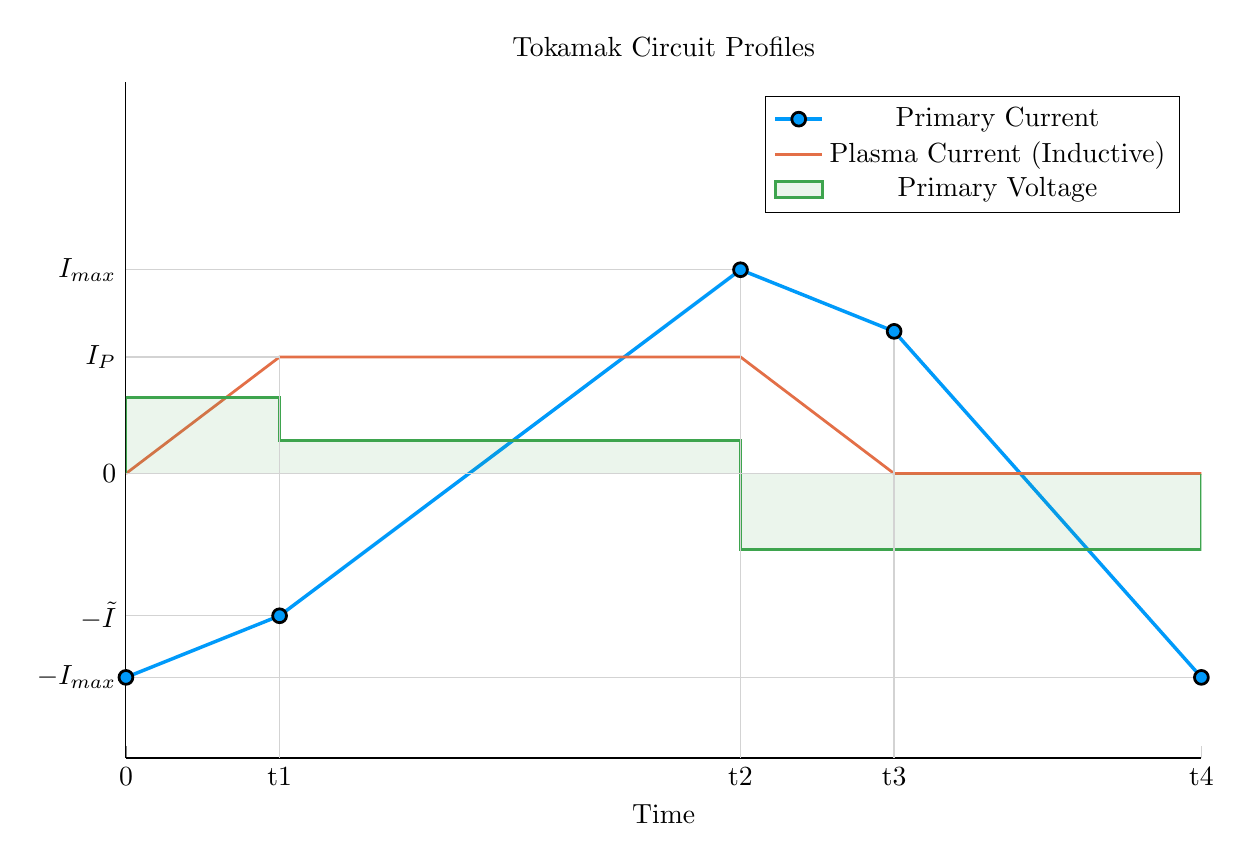
\begin{tikzpicture}[]
\begin{axis}[height = {101.6mm}, ylabel = {}, title = {Tokamak Circuit Profiles}, xmin = {0}, xmax = {7}, ymax = {4.125}, xlabel = {Time}, unbounded coords=jump,scaled x ticks = false,xticklabel style={rotate = 0},xmajorgrids = false,xtick = {0,1,4,5,7},xticklabels = {0,t1,t2,t3,t4},xtick align = inside,axis lines* = left,scaled y ticks = false,yticklabel style={rotate = 0},ymajorgrids = false,ytick = {0.0,-2.15,2.15,1.23,-1.5},yticklabels = {0,${-I_{max}}$,$I_{max}$,$I_P$,${-\tilde{I}}$},ytick align = inside,axis lines* = left,    xshift = 0.0mm,
    yshift = 0.0mm,
    axis background/.style={fill={rgb,1:red,1.00000000;green,1.00000000;blue,1.00000000}}
, ymin = {-3}, width = {152.4mm}]\addplot+ [color = {rgb,1:red,0.00000000;green,0.60560316;blue,0.97868012},
draw opacity=1.0,
line width=1.25,
solid,mark = *,
mark size = 2.5,
mark options = {
    color = {rgb,1:red,0.00000000;green,0.00000000;blue,0.00000000}, draw opacity = 1.0,
    fill = {rgb,1:red,0.00000000;green,0.60560316;blue,0.97868012}, fill opacity = 1.0,
    line width = 1,
    rotate = 0,
    solid
}]coordinates {
(0.0, -2.15)
(1.0, -1.5)
(4.0, 2.15)
(5.0, 1.5)
(7.0, -2.15)
};
\addlegendentry{Primary Current}
\addplot+ [color = {rgb,1:red,0.88887350;green,0.43564919;blue,0.27812294},
draw opacity=1.0,
line width=1,
solid,mark = none,
mark size = 2.0,
mark options = {
    color = {rgb,1:red,0.00000000;green,0.00000000;blue,0.00000000}, draw opacity = 1.0,
    fill = {rgb,1:red,0.88887350;green,0.43564919;blue,0.27812294}, fill opacity = 1.0,
    line width = 1,
    rotate = 0,
    solid
}]coordinates {
(0.0, 0.0)
(1.0, 1.23)
(4.0, 1.23)
(5.0, 0.0)
(7.0, 0.0)
};
\addlegendentry{Plasma Current (Inductive)}
\addplot+ [color = {rgb,1:red,0.24222430;green,0.64327509;blue,0.30444865},
draw opacity=1.0,
line width=1,
solid,mark = none,
mark size = 2.0,
mark options = {
    color = {rgb,1:red,0.00000000;green,0.00000000;blue,0.00000000}, draw opacity = 1.0,
    fill = {rgb,1:red,0.24222430;green,0.64327509;blue,0.30444865}, fill opacity = 1.0,
    line width = 1,
    rotate = 0,
    solid
},fill = {rgb,1:red,0.24222430;green,0.64327509;blue,0.30444865}, fill opacity=0.1,area legend]coordinates {
(0.0, 0.0)
(0.0, 0.8)
(1.0, 0.8)
(1.0, 0.35)
(4.0, 0.35)
(4.0, 0.0)
(NaN, NaN)
(4.0, 0.0)
(4.0, -0.8)
(7.0, -0.8)
(7.0, 0.0)
};
\addlegendentry{Primary Voltage}
\addplot+ [color = {rgb,1:red,0.82745098;green,0.82745098;blue,0.82745098},
draw opacity=1.0,
line width=0.5,
solid,mark = none,
mark size = 2.0,
mark options = {
    color = {rgb,1:red,0.00000000;green,0.00000000;blue,0.00000000}, draw opacity = 1.0,
    fill = {rgb,1:red,0.76444018;green,0.44411178;blue,0.82429754}, fill opacity = 1.0,
    line width = 1,
    rotate = 0,
    solid
},forget plot]coordinates {
(1.0, -4.25)
(1.0, 1.23)
(NaN, NaN)
(4.0, -4.25)
(4.0, 2.15)
(NaN, NaN)
(5.0, -4.25)
(5.0, 1.5)
(NaN, NaN)
(0.0, 1.23)
(1.0, 1.23)
(NaN, NaN)
(0.0, 2.15)
(4.0, 2.15)
(NaN, NaN)
(0.0, -1.5)
(1.0, -1.5)
(NaN, NaN)
(0.0, 0.0)
(5.0, 0.0)
(NaN, NaN)
(0.0, -2.15)
(7.0, -2.15)
};
\end{axis}

\end{tikzpicture}

\end{adjustbox}

\caption{Time Evolution of Circuit Profiles}
\label{fig:circuit_profiles} ~\\
\small{A circuit pulse involves four phases: (1) Ramp-Up, (2) Flattop, (3) Ramp-Down, and (4) Dwell. In reality, flattop can last more than 90\% of the pulse.\cite{inputfile} This makes the slope of the primary current during this phase much shallower than shown. }
\end{figure}

Transformer pulses between the central solenoid and the plasma occur on the timescale of hours. \added{During this time, a plasma is brought up to some quasi-steady-state current ($I_P^*$) for \replaced{several}{around an} hour and then ramped back down using the available flux in the solenoid (measured in volt-seconds).} For clarity, each pulse is subdivided into four phases: ramp-up, flattop, ramp-down, and dwell. Pictorially represented in \cref{fig:circuit_profiles}, these divisions allow a simple scheme for transforming the coupled circuit differential equations -- from \cref{eq:circ1,eq:circ2} -- into simple algebraic formulas. 

Along the way, we will approximate derivatives with linear piecewise functions. Using $t_i$ to represent the initial time and $t_f$ as the final one, these can be written as:
\begin{equation}
	\dot I = \frac{ I(t_f) - I(t_i) }{t_f - t_i}
\end{equation}
In tabular form, the data from \cref{fig:circuit_profiles} can be written in this piecewise fashion as:

\begin{table}[h!]
\centering	
\caption{Piecewise Linear Scheme for Pulsed Operation}
\hfill
\begin{subtable}[t]{0.4\textwidth}
\centering	
\caption{Currents} ~\\
\begin{tabular}{ c|c|c } 

\textbf{Time} & {$\bold{I_1}$} & {$\bold{I_2}$} \\
\hline
0 & $-I_{max}$ & 0 \\ 
t1 & $-\tilde I \ \ \ \,\, $ & $I_P^{\,*} $ \\ 
t2 & $+I_{max}$ & $I_P^{\,*}$ \\ 
t3 & $+\tilde I \ \ \ \,\, $ & 0 \\ 
t4 & $-I_{max}$ & 0 \\ 
\end{tabular}
\end{subtable}
\hfill
\begin{subtable}[t]{0.5\textwidth}
\centering	
\caption{Voltage} ~\\
\begin{tabular}{ c|c|c|c } 
\textbf{Phase} & $\bold{t_i}$ & $\bold{t_f}$ & $\bold{V_1}$ \\
\hline
Ramp-Up & 0 & $t_1$ & $+V_{max}$ \\ 
Flattop & $t_1$ & $t_2$ & $+ \tilde V$ \ \,\,\, \\ 
Ramp-Down & $t_2$ & $t_3$ & ${-V}_{max}$ \\ 
Dwell & $t_3$ & $t_4$ & ${-V}_{max}$ \\ 
\end{tabular}
\end{subtable}
\hfill
\hfill
\end{table}

\added{The exact definitions for the plasma's inductive current ($I_P^*$) and the maximum voltage in the central solenoid ($V_{max}$) will be put off until the end of the section.}

\subsubsection{The Ramp-Up Phase -- RU}

The first phase in every plasma pulse is the ramp-up. During ramp-up, the central solenoid starts discharging from its fully charged values, as the plasma is brought to its quasi-steady-state current. As this occurs on the timescale of minutes -- not hours -- resistive effects of the plasma can safely be ignored. This results in the ramp-up equations becoming:

\begin{align}
	V_{max} = \frac{1}{\tau_{RU}} \cdot \left( L_1 \cdot ( I_{max} - \tilde I ) - M \cdot I_{ID} \right) \\
	0 = \frac{1}{\tau_{RU}} \cdot \left( M \cdot ( I_{max} - \tilde I ) - L_2 \cdot I_{ID} \right)
\end{align}

Simplifying these equations will be done shortly, for now the new terms are what is important. The maximum voltage of the solenoid is $V_{max}$ \added{-- usually measured in kilovolts}. Next, $I_{max}$ is the solenoid's current at the beginning of ramp-up. Whereas $\tilde I$ is the magnitude of the current once the plasma is at its flattop inductive-drive current -- $I_{ID}$. The $\tau_{RU}$ quantity, then, is the duration of time it takes to ramp-up (i.e.\ RU). Again, $L_1$ and $L_2$ are the \added{microhenry-scale} internal inductances of the solenoid and plasma, respectively, and M is the mutual inductance between them.

The last step in discussing ramp-up is giving the two important formulas that come from it:
\begin{equation}
	\label{eq:itilde}
	\tilde I = I_{max} - I_{ID} \cdot \left( \frac{L_2}{M} \right)
\end{equation}
\begin{equation}
	\label{eq:tauru}
	\tau_{RU} = \frac{I_{ID}}{V_{max}} \cdot \left( \frac{ L_1 L_2 - M^2 }{ M } \right)
\end{equation}

\subsubsection{The Flattop Phase -- FT}

The most important phase in any reactor's pulse is flattop -- the quasi-steady-state time when the tokamak is making \replaced{electricity.}{electricity (and money).} Flattops are assumed to last a couple of hours for a profitable machine, during which the central solenoid completely discharges to overcome a plasma's resistive losses -- keeping it in a quasi-steady-state mode of operation. In a steady-state reactor, this phases constitutes the entirety of the pulse.

Although the resistance cannot be safely neglected for flattop -- as it was for ramp-up -- the plasma's inductive current ($I_{ID}$) is assumed constant. This leads to its derivative in equations cancelling out! Mathematically,

\begin{align}
	\tilde V = \frac{L_1}{\tau_{FT}} \cdot \left( I_{max} + \tilde I \right) \\
	I_{ID} R_P = \frac{M}{\tau_{FT}} \cdot \left( I_{max} + \tilde I \right)
\end{align}

As with ramp-up, the simplifications will be given shortly. The new terms here, however, are an intermediate voltage for the central solenoid ($\tilde V$), and the duration of the flattop ($\tau_{FT}$). The resistance term was given in \cref{eq:rp}. Solutions can then be found by substituting $\tilde I$ -- from \cref{eq:itilde} -- into the flattop equations:
\begin{equation}
	\tilde V = I_{ID} R_P \cdot \left( \frac{L_1}{M} \right)	
\end{equation}
\begin{equation}
	\label{eq:tauft}
	\tau_{FT} = \frac{ I_{max} \cdot 2 M - I_{ID} \cdot  L_2 }{I_{ID} R_P}
\end{equation}

\subsubsection{The Ramp-Down Phase -- RD}

Due to the simplicity -- and symmetry -- of this model's reactor pulse, ramp-down is the exact mirror of ramp-up. It takes the same amount of time and results in the same algebraic equations. For brevity, this will just be represented as:
\begin{equation}
	\label{eq:taurd}
	\tau_{RD} = \tau_{RU}
\end{equation}
For clarity, this is the time when a plasma's current is brought down from its flattop value to zero.

\subsubsection{The Dwell Phase -- DW}

Where the first three phases had little ambiguity, the dwell phase changes definition from model to model. For now, it is assumed to be the time it takes the central solenoid to reset after a plasma has been completely ramped-down to an off-mode. To get a more realistic duty factor for cost estimates, it could include an evacuation time, set to last around thirty minutes. During this evacuation, a plasma is vacuumed out of a device as it undergoes some inter-pulse maintenance.

Ignoring evacuation for now, the dwell phase involves resetting the central solenoid when the plasma's current is negligible. This \deleted{fundamentally} means the secondary of the transformer is \replaced{an open circuit}{nonexistent} -- \added{fundamentally} the central solenoid is the \replaced{only component.}{entire circuit.} In equation form,
\begin{equation}
	V_{max} = \frac{L_1}{\tau_{DW}} \cdot \left( I_{max} + \tilde I \right) 
\end{equation}
Or substituting in $\tilde I$ and solving for $\tau_{DW}$,
\begin{equation}
	\label{eq:taudw}
	\tau_{DW} = \frac{L_1}{M} \cdot \frac{ \left( I_{max} \cdot 2 M - I_{ID} \cdot  L_2 \right) }{V_{max}}
\end{equation}

\subsection{Specifying Circuit Variables}

The goal now is to collect the results from the four phases and introduce the inductance, resistance, voltage, and current terms relevant to our model. This will motivate recasting the problem as flux balance in a reactor -- the form commonly used in the literature (and discussed next section).

First, collecting the phase durations in one place:

\begin{align}
	\tag{\ref{eq:tauru}}
	\tau_{RU} &= \frac{I_{ID}}{V_{max}} \cdot \left( \frac{ L_1 L_2 - M^2 }{ M } \right) \\
	\tag{\ref{eq:tauft}}
	\tau_{FT} &= \frac{ I_{max} \cdot 2 M - I_{ID} \cdot  L_2 }{I_{ID} R_P} \\
	\tag{\ref{eq:taurd}}
	\tau_{RD} &= \tau_{RU} \\
	\tag{\ref{eq:taudw}}
	\tau_{DW} &= \frac{L_1}{M} \cdot \frac{ \left( I_{max} \cdot 2 M - I_{ID} \cdot  L_2 \right) }{V_{max}}
\end{align}

These can be used in the definition of the duty-factor: the fraction of time a reactor is putting electricity on the grid. Formulaically,
\begin{equation}
	\label{eq:duty}
	f_{duty} = \frac{\tau_{FT}}{\tau_{pulse}}
\end{equation}
\begin{equation}
	\tau_{pulse} = \tau_{RU} + \tau_{FT} + \tau_{RD} + \tau_{DW}
\end{equation}
As will turn out, the solving of pulsed current actually only involves \cref{eq:tauft}. What is interesting about this, is that there is no explicit dependence on ramp-down or dwell! Whereas ramp-up passes $\tilde I$ to the flattop phase, the other two are just involved in calculating the duty factor.

The remainder of this subsection will then be defining the following circuit variables: $I_{ID}$, $I_{max}$, $V_{max}$, $L_1$, $L_2$, and $M$. Again, the resistance was defined last chapter as:
\begin{equation}
	\tag{\ref{eq:rp}}
	R_P = \frac{K_{RP}}{R_0 \overline T ^ {3/2}}
\end{equation}

\subsubsection{The Inductive Current -- $I_{ID}$}

The inductive current is the source of current that separates pulsed from steady-state operation. Quickly fitting it into the previous definitions of current balance -- see \cref{eq:ifbal}:
\begin{equation}
	I_{ID} = I_P - ( I_{BS} + I_{CD} )
\end{equation}
As before, $I_P$ is the total plasma current in mega-amps, $I_{BS}$ is the bootstrap current, and $I_{CD}$ is the current from LHCD (i.e.\ lower hybrid current drive). For this model, the relation can be rewritten as:
\begin{equation}
	I_{ID} = I_P \cdot \Big( 1 - K_{CD} ( \sigma v ) \Big) - K_{BS} \, \overline T
\end{equation}

\subsubsection{The Central Solenoid Maximums -- $V_{max}$ and $I_{max}$}

For this simple model, the central solenoid has two maximum values: the voltage and current. The voltage is the easier to give value. Literature values have this around: \cite{arc}
\begin{equation}
	V_{max} \approx 5 \, \textnormal{kV}
\end{equation}
The maximum current, on the other hand, can be defined through Ampere's Law on a helically-shaped central solenoid: \cite{griffiths}
\begin{equation}
	I_{max} = \frac{B_{CS} h_{CS}}{N \mu_0}
\end{equation}
Here, $B_{CS}$ is a magnetic field strength the central solenoid is assumed to operate at (i.e.\ 12 T), $h_{CS}$ is the height of the solenoid, N is the number of loops, and $\mu_0$ has its usual physics meaning $\left( \textnormal{i.e.\ } \ 40 \, \pi \, \frac{ \mu \textnormal{H}}{\textnormal{m}} \right)$. As will be seen, the value of N does not directly affect the model, as it cancels out in the final flux balance. The height of the central solenoid will be the focus of an upcoming section on improving tokamak geometry.

\subsubsection{The Central Solenoid Inductance -- $L_1$}

For a central solenoid with circular cross-sections of finite thickness (d), the inductance can be written as: \cite{hartmann}
\begin{equation}
	L_1 = G_{LT} \cdot \left( \frac{\mu_0 \pi N^2}{h_{CS}} \right)
\end{equation}
\begin{equation}
	G_{LT} = \frac{R_{CS}^2 + R_{CS} \cdot ( R_{CS} + d ) + ( R_{CS} + d ) ^ 2 }{3}
\end{equation}
Note that $R_{CS}$ is the inner radius of the central solenoid and $( R_{CS} + d )$ is the outer one. In the limit where d is negligible, this says that the inductance is quadratically dependent on the radius of the central solenoid:
\begin{equation}
	\label{eq:glt_simple}
	\underset{d \to 0}{\lim} \ G_{LT} = G_{LT}^{\,\dagger} = R_{CS}^2
\end{equation}
The formulas for both $R_{CS}$ and d will be defined in a few sections.

\subsubsection{The Plasma Inductance -- $L_2$}

The plasma inductance is a composite of several different terms, but overall scales with radius. Through equation,
\begin{equation}
	L_2 = K_{LP} R_0
\end{equation}
This \replaced{static}{fixed} coefficient -- $K_{LP}$ -- then combines three inductive behaviors of the plasma. The first is its own self inductance (through $l_i$). \cite{jeff} The next is a resistive component through the Ejima coefficient, $C_{ejima}$, which is usually set to $\sim \frac{1}{3}$. \cite{process} And lastly, a geometric component -- involving $\epsilon$ and $\kappa$ -- is given by the Hirshman-Neilson model. \cite{hn85} Mathematically,
\begin{equation}
	K_{LP} = \mu_0 \cdot \left( \frac{l_i}{2} + C_{ejima} + \frac{ ( b_{HN} - a_{HN} ) \, ( 1 - \epsilon ) }{ ( 1 - \epsilon ) + \kappa \, d_{HN} } \right)
\end{equation}
Here the HN values come from the 1985 Hirshman-Neilson paper:
\begin{equation}
	a_{HN}(\epsilon) = 2.0 + 9.25 \sqrt{\epsilon} - 1.21 \, \epsilon
\end{equation}
\begin{equation}
	b_{HN}(\epsilon) = \textnormal{ln} (8/\epsilon) \cdot ( 1 + 1.81 \sqrt{\epsilon} + 2.05 \, \epsilon )
\end{equation}
\begin{equation}
	d_{HN}(\epsilon) = 0.73 \sqrt{\epsilon}  \cdot ( 1 + 2 \epsilon^4 - 6 \epsilon^5 +3.7 \epsilon^6 )
\end{equation}

\subsubsection{The Mutual Inductance -- M}

The mutual inductance -- M -- represents the coupling between the solenoid primary and the plasma secondary. A common method for treating this mutual inductance is through a coupling coefficient, k, that links the two self-inductances. Formulaically, 
\begin{equation}
	M = k \sqrt{ L_1 L_2 }
\end{equation}
The value of the coupling coefficient, k, is always less than (or equal to) 1, but usually has a value around one-third. With all the equations defined, we are now at a position to explain one of the larger nuances of this fusion systems framework: declaring the pulse length of a tokamak.

\subsection{\replaced{Constructing}{Reasoning} the Pulse Length}

\label{section:pulse}

This subsection focuses on a quantitative estimate for how to select a pulse length. As no fusion reactor exists in the world today, the writers believe this is an acceptable calculation. Further, the resulting length of two hours matches the durations of other studies in the literature.

Starting at the end, our goal is to find the pulse length of a tokamak reactor in seconds \added{-- as dictated by cyclical stress concerns}.  The first piece of information is the expected lifetime of the central solenoid, $ N \approx 10 \ \textnormal{years} $. The next is the desired number of \replaced{pulses}{shots} the \replaced{central solenoid will have to last:}{machine will likely have,} $ M \approx 50,000 \ \textnormal{pulses} $.\footnote{This 50,000 pulses is based on the values from the ITER design specifications.\cite{iter_cs} } This gives the \replaced{rough}{ballpark} estimate of around 10 pulses a day -- or a \added{flattop} pulse length of two hours.

With the pulse length defined, we are now in a position to justify neglecting the duty factor for pulsed reactors in this model. Using \replaced{expected}{ballpark} reactor values -- while assuming the central solenoid has around 4000 turns -- leads to the following scalings:
\begin{equation}
	\tau_{FT} \sim \tau_{pulse} \sim \textnormal{O(hours)}
\end{equation}
\begin{equation}
	\tau_{RU} \sim \tau_{RD} \sim \tau_{DW} \sim \textnormal{O(mins)}
\end{equation}
As such, even pulsed tokamak reactors should have a duty factor of around unity:
\begin{equation}
	f_{duty} \approx 1
\end{equation}
\added{This analysis of course would change if the central solenoid became an inexpensive component to replace. For example, if a tokamak had a new one installed annually, the pulse length could shorten to be on the order of minutes.}

Now that all the terms in a pulsed circuit have been explored, we will move on to rearranging the flattop equation to reproduce flux balance. This will then naturally lead to a generalized current equation -- which is the main result of the chapter.

\section{\replaced{Producing}{Salvaging} Flux Balance}

The goal of this section is to arrive at a conservation equation for flux balance that mirrors the ones in the literature. The fusion systems model this one attempts to follow most is the PROCESS code.\cite{process} In a manner similar to power balance, flux balance can be written as:
\begin{equation}
	\sum_{sources} \Phi = \sum_{sinks} \, \Phi
\end{equation}

\subsection{Rearranging the Circuit Equation}

The way to arrive at flux balance from the circuit equation is to rearrange the flattop phase's duration equation:
\begin{equation}
	\tag{\ref{eq:tauft}}
	\tau_{FT} = \frac{ I_{max} \cdot 2 M - I_{ID} \cdot  L_2 }{I_{ID} R_P}
\end{equation}
Multiplying by the right-hand side's denominator and moving the negative term over yields:
\begin{equation}
	2 M I_{max} = I_{ID} \cdot \left( L_2 + R_P \tau_{FT} \right) 
\end{equation}
This equation is flux balance, where the left-hand side are the sources (e.g.\ the central solenoid), and the other terms are the sinks (i.e.\ ramp-up and flattop). The source term can currently be encapsulated in:
\begin{equation}
	\label{eq:phics}
	\Phi_{CS} = 2 M I_{max}
\end{equation}
The sinks, namely the ramp-up inductive losses ($\Phi_{RU}$) and the flattop resistive losses ($\Phi_{FT}$), are what drain up the flux. Again, ramp-down and dwell are not included as sinks because flux balance only tracks till the end of flattop. They come into play when measuring the cost of electricity -- through the duty factor from \cref{eq:duty}.

Relabeling terms, flux balance can now be rewritten as:
\begin{equation}
	\Phi_{CS} = \Phi_{RU} + \Phi_{FT}
\end{equation}
With the ramp-up and flattop flux given respectively by:
\begin{equation}
	\label{eq:phiru}
	\Phi_{RU} = L_2 \cdot I_{ID}
\end{equation}
\begin{equation}
	\label{eq:phift}
	\Phi_{FT} = ( R_P \tau_{FT} ) \cdot I_{ID}
\end{equation}
On comparing these quantities to the ones from the PROCESS team, $\Phi_{RU}$ and $\Phi_{FT}$ are exactly the same. The source terms, on the other hand, are off for two reasons -- both related to the central solenoid being the only source term in flux balance. This can partially be remedied by adding the second most dominant source of flux a posteriori -- i.e.\ the PF coils. The second, and inherently limiting factor, is the simplicity of the current model. All that can be shown to this regard is that the $\Phi_{CS}$ terms does reasonably predict the values from \added{the} PROCESS \added{code}.

\subsection{\replaced{Adding}{Importing} Poloidal Field Coils}

Adding the effect of PF coils -- belts of current driving plates on the outer edges of the tokamak -- leads to \replaced{as much as a 50\% improvement\cite{process,inputfile}}{a second-order improvement} over relying solely on the central solenoid for flux generation. From the literature, this can be modeled as: \cite{hartmann}
\begin{equation}
	\label{eq:phipf}
	\Phi_{PF} = \pi B_V \cdot \left( R_0^2 - ( R_{CS} + d ) ^ 2 \right)
\end{equation}
Where again $R_{CS}$ and $d$ are the inner radius and thickness of the central solenoid, respectively. These will be the topic of the next section.

Moving forward, the vertical field -- $B_V$ -- is a magnetic field oriented up-and-down with the ground. It is needed to prevent a tokamak plasma from \replaced{drifting radially}{spinning} out of the machine. From the literature, the magnitude of this vertical field \added{(valid for a circular plasma)} is given by: \cite{process}
\begin{equation}
  |B_V| = \frac{\mu_0 I_P}{4 \pi R_0} \cdot \left( \,\textnormal{ln} \left(\frac{8}{\epsilon}\right) + \beta_{\,p} + \frac{l_i}{2} - \frac{3}{2} \, \right)
\end{equation} 
Analogous to the previously covered plasma beta, the poloidal beta can be represented by: \cite{elongation}
\begin{equation}
  \beta_p = \frac{\overline{p}}{\left( \frac{\overline{B_p}^{\,2}}{2 \mu_0} \right)}
\end{equation}
Where the average poloidal magnetic field comes from a simple application of Ampere's law:
\begin{equation}
	\overline{B_p} = \frac{\mu_0 I_P}{l_p}
\end{equation}
The variable $l_p$ is then the perimeter of the tokamak's cross-sectional halves:
\begin{equation}
	l_p = 2 \pi a \cdot \sqrt{g_p}
\end{equation}
Here, $g_p$ is another geometric scaling factor,
\begin{equation}
  g_p = \frac{1 + \kappa^2 ( 1 + 2 \delta^2 - 1.2\delta^3 )}{2} 
\end{equation}
\replaced{After a few lines of algebra}{Boiled down}, this relation for the magnitude of the vertical magnetic field can be written in standardized units as:
\begin{equation}
	|B_V| = \left( \frac{ 1 }{ 10 \cdot R_0} \right) \cdot \left( K_{VI} I_P +  K_{VT\,} \overline{T}  \right)
\end{equation}
\begin{equation}
	K_{VT} = K_{n} \cdot ( \epsilon ^ 2 \, g_P ) \cdot ( 1 + f_D ) \, \frac{ (1 + \nu_n) \, (1 + \nu_T) }{1 + \nu_n + \nu_T }
\end{equation}
\begin{equation}
	K_{VI} = \textnormal{ln} \left(\frac{8}{\epsilon}\right) + \frac{l_i}{2} - \frac{3}{2}
\end{equation}
For clarity, this will be plugged into the new PF coil flux contribution ($\Phi_{PF}$):
\begin{equation}
	\tag{\ref{eq:phipf}}
	\Phi_{PF} = \pi B_V \cdot \left( R_0^2 - ( R_{CS} + d ) ^ 2 \right)
\end{equation}
Which then gets plugged into a more complete flux balance:
\begin{equation}
	\label{eq:full_ibal}
	\tcboxmath{
		\Phi_{CS} + \Phi_{PF} = \Phi_{RU} + \Phi_{FT}
	}
\end{equation}
The $R_{CS}$ and $d$ terms found in $\Phi_{PF}$ will now be discussed as they are needed for this more sophisticated tokamak geometry.

\section{Improving Tokamak Geometry}

From before, this fusion systems model has been said to depend on the major and minor radius -- $R_0$ and $a$, respectively -- and along the way, various geometric parameters have been defined (e.g.\ $\epsilon$, $\kappa$, $\delta$) to describe the geometry further. Now three more thicknesses will be added: $b$, $c$, and $d$. Additionally, two fundamental dimension corresponding to the solenoid will be given: the radius ($R_{CS}$) and height ($h_{CS}$). These are the topics of this section.

\subsection{Defining Central Solenoid Dimensions}

The best way to conceptualize tokamak geometry is through cartoon -- see \cref{fig:dims}. What this says is there is a gap at the very center of a tokamak. This gap extends radially outwards to $R_{CS}$ meters where the \replaced{spiraled}{slinky-shaped} central solenoid -- of thickness $d$ -- begins. Between the outer edge of the solenoid and the wall of the torus (i.e.\ the doughnut) are the blanket and toroidal field (TF) coils.

\begin{figure*}
\centering
\begin{adjustbox}{width=0.85\textwidth}
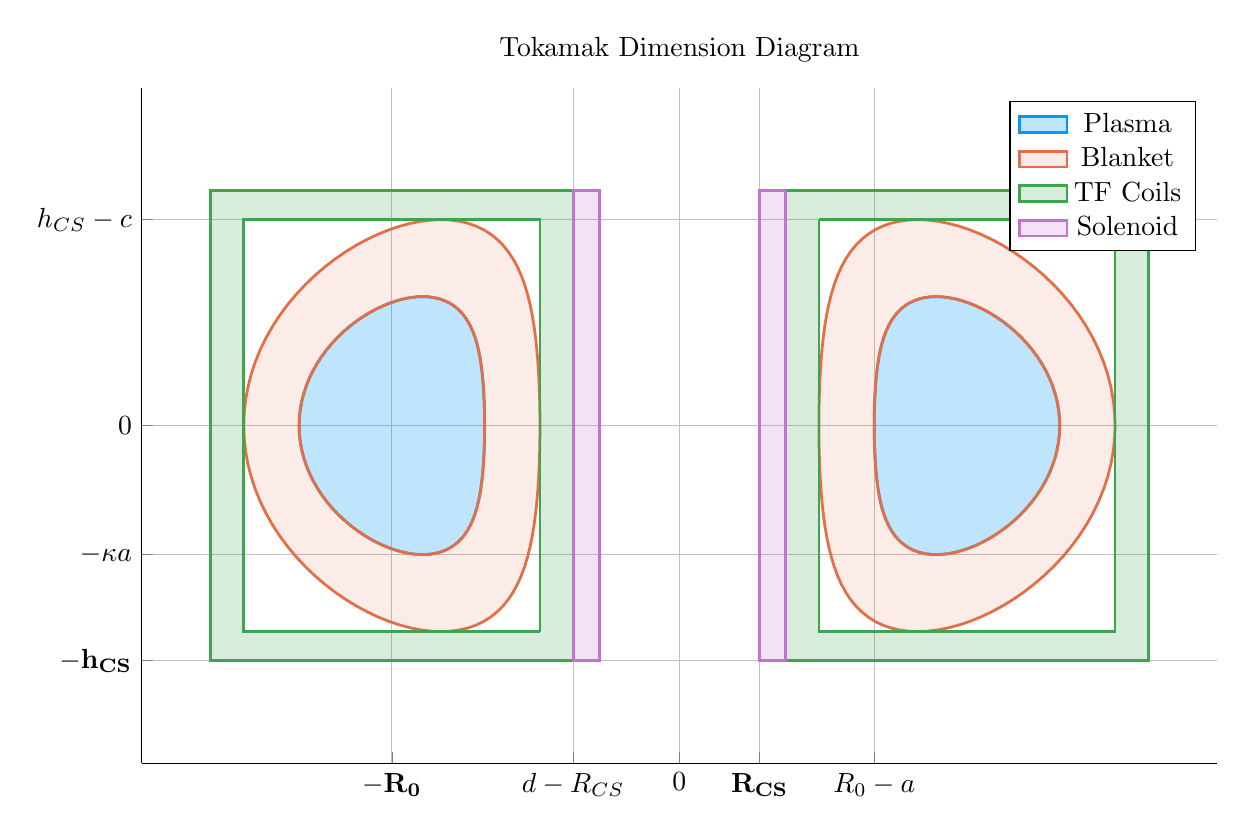
\begin{tikzpicture}[]
\begin{axis}[height = {101.6mm}, ylabel = {}, title = {Tokamak Dimension Diagram}, xmin = {-16.96464}, xmax = {16.96464}, ymax = {12.181706012903225}, xlabel = {}, unbounded coords=jump,scaled x ticks = false,xticklabel style={rotate = 0},xmajorgrids = true,xtick = {0.0,2.5317214541730677,-9.072,6.145548387096774,-3.3497214541730678},xticklabels = {0,$\bf{R_{CS}}$,$\bf{{-R}_0}$,$R_0 - a$,$d - R_{CS}$},xtick align = inside,axis lines* = left,scaled y ticks = false,yticklabel style={rotate = 0},ymajorgrids = true,ytick = {0.0,-8.478922887864822,-4.653058064516129,7.428922887864823},yticklabels = {0,$\bf{{-h}_{CS}}$,${-\kappa} a$,$h_{CS} - c$},ytick align = inside,axis lines* = left,    xshift = 0.0mm,
    yshift = 0.0mm,
    axis background/.style={fill={rgb,1:red,1.00000000;green,1.00000000;blue,1.00000000}}
, ymin = {-12.181706012903225}, width = {152.4mm}]\addplot+ [color = {rgb,1:red,0.00000000;green,0.60560316;blue,0.97868012},
draw opacity=1.0,
line width=1,
solid,mark = none,
mark size = 2.0,
mark options = {
    color = {rgb,1:red,0.00000000;green,0.00000000;blue,0.00000000}, draw opacity = 1.0,
    fill = {rgb,1:red,0.00000000;green,0.60560316;blue,0.97868012}, fill opacity = 1.0,
    line width = 1,
    rotate = 0,
    solid
},fill = {rgb,1:red,0.00000000;green,0.60560316;blue,0.97868012}, fill opacity=0.25,area legend]coordinates {
(-11.998451612903224, 0.0)
(-11.98922207919679, 0.2921679332710291)
(-11.961601612443932, 0.5831828131882695)
(-11.915794116436746, 0.8718961369727396)
(-11.852137762522407, 1.1571684850360338)
(-11.771102473770108, 1.4378740177488842)
(-11.673286377647635, 1.7129049186158334)
(-11.55941120568557, 1.9811757663208256)
(-11.430316617462449, 2.241627818389261)
(-11.286953428530017, 2.4932331895608506)
(-11.130375728034215, 2.7349989083831394)
(-10.96173188200961, 2.9659708360161865)
(-10.782254432669117, 3.1852374317826615)
(-10.59324892230544, 3.391933350602452)
(-10.396081692289423, 3.58524285811436)
(-10.192166732519574, 3.7644030500069485)
(-9.982951683794182, 3.9287068628533244)
(-9.769903124035281, 4.0775058645674545)
(-9.554491298062636, 4.21021281346937)
(-9.338174478579997, 4.326303975859794)
(-9.122383172034585, 4.425321192957779)
(-8.908504405883159, 4.5068736890441015)
(-8.697866352426912, 4.570639613674501)
(-8.491723557735288, 4.616367311876341)
(-8.2912430513685, 4.643876317315818)
(-8.097491612903225, 4.653058064516129)
(-7.911424464141755, 4.643876317315818)
(-7.73387564104738, 4.616367311876341)
(-7.565550276852846, 4.570639613674501)
(-7.4070189976483904, 4.506873689044102)
(-7.258714594546428, 4.42532119295778)
(-7.120931092970638, 4.326303975859795)
(-6.993825290693801, 4.21021281346937)
(-6.877420783129728, 4.077505864567455)
(-6.771614438426758, 3.928706862853325)
(-6.676185227609827, 3.7644030500069485)
(-6.590805257964794, 3.58524285811436)
(-6.515052802686304, 3.391933350602452)
(-6.448427068145589, 3.1852374317826624)
(-6.390364393542622, 2.9659708360161874)
(-6.340255537642832, 2.73499890838314)
(-6.297463675055492, 2.4932331895608506)
(-6.261342701178994, 2.241627818389261)
(-6.231255431364441, 1.9811757663208265)
(-6.206591276608178, 1.7129049186158343)
(-6.186782985455325, 1.4378740177488847)
(-6.171322059752492, 1.1571684850360338)
(-6.159772480089943, 0.8718961369727395)
(-6.151782414579849, 0.5831828131882707)
(-6.147093631099405, 0.29216793327103)
(-6.145548387096774, 5.698352664956456e-16)
(-6.147093631099405, -0.2921679332710289)
(-6.151782414579849, -0.5831828131882696)
(-6.159772480089943, -0.8718961369727383)
(-6.171322059752492, -1.1571684850360326)
(-6.1867829854553245, -1.4378740177488838)
(-6.206591276608178, -1.7129049186158334)
(-6.231255431364441, -1.9811757663208256)
(-6.261342701178992, -2.2416278183892597)
(-6.297463675055493, -2.4932331895608497)
(-6.340255537642832, -2.734998908383139)
(-6.390364393542622, -2.9659708360161865)
(-6.448427068145589, -3.185237431782662)
(-6.515052802686304, -3.3919333506024514)
(-6.590805257964794, -3.5852428581143605)
(-6.676185227609827, -3.7644030500069485)
(-6.771614438426755, -3.928706862853323)
(-6.877420783129727, -4.0775058645674545)
(-6.9938252906938, -4.21021281346937)
(-7.120931092970639, -4.326303975859795)
(-7.258714594546428, -4.425321192957779)
(-7.407018997648389, -4.5068736890441015)
(-7.565550276852846, -4.570639613674501)
(-7.733875641047377, -4.616367311876341)
(-7.9114244641417555, -4.643876317315818)
(-8.097491612903225, -4.653058064516129)
(-8.291243051368498, -4.643876317315818)
(-8.491723557735288, -4.616367311876341)
(-8.69786635242691, -4.570639613674501)
(-8.90850440588316, -4.5068736890441015)
(-9.122383172034585, -4.42532119295778)
(-9.338174478579994, -4.326303975859796)
(-9.554491298062636, -4.21021281346937)
(-9.76990312403528, -4.077505864567455)
(-9.982951683794184, -3.928706862853324)
(-10.192166732519574, -3.7644030500069494)
(-10.396081692289421, -3.5852428581143614)
(-10.59324892230544, -3.391933350602452)
(-10.782254432669115, -3.1852374317826624)
(-10.96173188200961, -2.9659708360161865)
(-11.130375728034215, -2.7349989083831403)
(-11.286953428530017, -2.493233189560853)
(-11.430316617462449, -2.241627818389261)
(-11.559411205685569, -1.981175766320827)
(-11.673286377647635, -1.7129049186158327)
(-11.771102473770108, -1.4378740177488853)
(-11.852137762522407, -1.1571684850360362)
(-11.915794116436746, -0.8718961369727398)
(-11.961601612443932, -0.5831828131882713)
(-11.98922207919679, -0.2921679332710286)
(-11.998451612903224, -1.1396705329912913e-15)
(NaN, NaN)
(11.998451612903224, 0.0)
(11.98922207919679, 0.2921679332710291)
(11.961601612443932, 0.5831828131882695)
(11.915794116436746, 0.8718961369727396)
(11.852137762522407, 1.1571684850360338)
(11.771102473770108, 1.4378740177488842)
(11.673286377647635, 1.7129049186158334)
(11.55941120568557, 1.9811757663208256)
(11.430316617462449, 2.241627818389261)
(11.286953428530017, 2.4932331895608506)
(11.130375728034215, 2.7349989083831394)
(10.96173188200961, 2.9659708360161865)
(10.782254432669117, 3.1852374317826615)
(10.59324892230544, 3.391933350602452)
(10.396081692289423, 3.58524285811436)
(10.192166732519574, 3.7644030500069485)
(9.982951683794182, 3.9287068628533244)
(9.769903124035281, 4.0775058645674545)
(9.554491298062636, 4.21021281346937)
(9.338174478579997, 4.326303975859794)
(9.122383172034585, 4.425321192957779)
(8.908504405883159, 4.5068736890441015)
(8.697866352426912, 4.570639613674501)
(8.491723557735288, 4.616367311876341)
(8.2912430513685, 4.643876317315818)
(8.097491612903225, 4.653058064516129)
(7.911424464141755, 4.643876317315818)
(7.73387564104738, 4.616367311876341)
(7.565550276852846, 4.570639613674501)
(7.4070189976483904, 4.506873689044102)
(7.258714594546428, 4.42532119295778)
(7.120931092970638, 4.326303975859795)
(6.993825290693801, 4.21021281346937)
(6.877420783129728, 4.077505864567455)
(6.771614438426758, 3.928706862853325)
(6.676185227609827, 3.7644030500069485)
(6.590805257964794, 3.58524285811436)
(6.515052802686304, 3.391933350602452)
(6.448427068145589, 3.1852374317826624)
(6.390364393542622, 2.9659708360161874)
(6.340255537642832, 2.73499890838314)
(6.297463675055492, 2.4932331895608506)
(6.261342701178994, 2.241627818389261)
(6.231255431364441, 1.9811757663208265)
(6.206591276608178, 1.7129049186158343)
(6.186782985455325, 1.4378740177488847)
(6.171322059752492, 1.1571684850360338)
(6.159772480089943, 0.8718961369727395)
(6.151782414579849, 0.5831828131882707)
(6.147093631099405, 0.29216793327103)
(6.145548387096774, 5.698352664956456e-16)
(6.147093631099405, -0.2921679332710289)
(6.151782414579849, -0.5831828131882696)
(6.159772480089943, -0.8718961369727383)
(6.171322059752492, -1.1571684850360326)
(6.1867829854553245, -1.4378740177488838)
(6.206591276608178, -1.7129049186158334)
(6.231255431364441, -1.9811757663208256)
(6.261342701178992, -2.2416278183892597)
(6.297463675055493, -2.4932331895608497)
(6.340255537642832, -2.734998908383139)
(6.390364393542622, -2.9659708360161865)
(6.448427068145589, -3.185237431782662)
(6.515052802686304, -3.3919333506024514)
(6.590805257964794, -3.5852428581143605)
(6.676185227609827, -3.7644030500069485)
(6.771614438426755, -3.928706862853323)
(6.877420783129727, -4.0775058645674545)
(6.9938252906938, -4.21021281346937)
(7.120931092970639, -4.326303975859795)
(7.258714594546428, -4.425321192957779)
(7.407018997648389, -4.5068736890441015)
(7.565550276852846, -4.570639613674501)
(7.733875641047377, -4.616367311876341)
(7.9114244641417555, -4.643876317315818)
(8.097491612903225, -4.653058064516129)
(8.291243051368498, -4.643876317315818)
(8.491723557735288, -4.616367311876341)
(8.69786635242691, -4.570639613674501)
(8.90850440588316, -4.5068736890441015)
(9.122383172034585, -4.42532119295778)
(9.338174478579994, -4.326303975859796)
(9.554491298062636, -4.21021281346937)
(9.76990312403528, -4.077505864567455)
(9.982951683794184, -3.928706862853324)
(10.192166732519574, -3.7644030500069494)
(10.396081692289421, -3.5852428581143614)
(10.59324892230544, -3.391933350602452)
(10.782254432669115, -3.1852374317826624)
(10.96173188200961, -2.9659708360161865)
(11.130375728034215, -2.7349989083831403)
(11.286953428530017, -2.493233189560853)
(11.430316617462449, -2.241627818389261)
(11.559411205685569, -1.981175766320827)
(11.673286377647635, -1.7129049186158327)
(11.771102473770108, -1.4378740177488853)
(11.852137762522407, -1.1571684850360362)
(11.915794116436746, -0.8718961369727398)
(11.961601612443932, -0.5831828131882713)
(11.98922207919679, -0.2921679332710286)
(11.998451612903224, -1.1396705329912913e-15)
};
\addlegendentry{Plasma}
\addplot+ [color = {rgb,1:red,0.88887350;green,0.43564919;blue,0.27812294},
draw opacity=1.0,
line width=1,
solid,mark = none,
mark size = 2.0,
mark options = {
    color = {rgb,1:red,0.00000000;green,0.00000000;blue,0.00000000}, draw opacity = 1.0,
    fill = {rgb,1:red,0.88887350;green,0.43564919;blue,0.27812294}, fill opacity = 1.0,
    line width = 1,
    rotate = 0,
    solid
},fill = {rgb,1:red,0.88887350;green,0.43564919;blue,0.27812294}, fill opacity=0.125,area legend]coordinates {
(-13.74427854582693, 0.0)
(-13.72954296908463, 0.46646592767223927)
(-13.685445019996358, 0.9310909274359673)
(-13.612310244800092, 1.392041336684088)
(-13.510678556994915, 1.8474979947395098)
(-13.381300220642846, 2.2956634222512418)
(-13.225130186826302, 2.734768915024204)
(-13.04332074889991, 3.1630815242866377)
(-12.837212480347718, 3.5789108958472036)
(-12.608323422706404, 3.9806159411507194)
(-12.358336500812388, 4.3666113139049525)
(-12.08908515895104, 4.735373666718153)
(-11.802537234387401, 5.08544766305526)
(-11.500777113966619, 5.4154517207863275)
(-11.185986254387002, 5.724083464660006)
(-10.860422186454013, 6.010124866183653)
(-10.526396166917667, 6.272447050625345)
(-10.18624968693083, 6.510014752166694)
(-9.842330092097374, 6.721890399624077)
(-9.496965613725703, 6.907237816613755)
(-9.152440152411872, 7.065325521558049)
(-8.81096819159381, 7.195529614508949)
(-8.474670248460548, 7.297336239396166)
(-8.14554929092694, 7.370343611982296)
(-7.825468560863273, 7.4142636055216355)
(-7.516131244239631, 7.428922887864823)
(-7.2190624174706315, 7.4142636055216355)
(-6.935593675557043, 7.370343611982296)
(-6.666850811544881, 7.297336239396167)
(-6.4137448687014755, 7.195529614508949)
(-6.176966827400615, 7.065325521558051)
(-5.956986119179431, 6.907237816613756)
(-5.754053082320152, 6.721890399624076)
(-5.568205388501765, 6.510014752166695)
(-5.3992783807260825, 6.272447050625345)
(-5.246919171238659, 6.010124866183653)
(-5.110604257075394, 5.724083464660006)
(-4.989660322779391, 5.4154517207863275)
(-4.88328781734585, 5.085447663055262)
(-4.790586818065825, 4.735373666718154)
(-4.7105846299742, 4.366611313904953)
(-4.642264518129107, 3.9806159411507194)
(-4.584594932698949, 3.578910895847203)
(-4.536558565161822, 3.1630815242866395)
(-4.497180568747824, 2.7347689150242047)
(-4.465555288023927, 2.2956634222512426)
(-4.440870871189059, 1.8474979947395103)
(-4.422431183673739, 1.3920413366840876)
(-4.409674501998921, 0.9310909274359696)
(-4.402188541060726, 0.46646592767224077)
(-4.399721454173068, 9.097806635736167e-16)
(-4.402188541060726, -0.466465927672239)
(-4.409674501998921, -0.9310909274359678)
(-4.422431183673739, -1.392041336684086)
(-4.440870871189059, -1.8474979947395083)
(-4.465555288023926, -2.295663422251241)
(-4.497180568747823, -2.734768915024204)
(-4.536558565161822, -3.1630815242866377)
(-4.5845949326989475, -3.5789108958472013)
(-4.642264518129108, -3.980615941150719)
(-4.7105846299742, -4.3666113139049525)
(-4.790586818065825, -4.735373666718153)
(-4.88328781734585, -5.085447663055261)
(-4.989660322779391, -5.415451720786327)
(-5.110604257075395, -5.724083464660007)
(-5.246919171238659, -6.010124866183653)
(-5.399278380726081, -6.272447050625343)
(-5.568205388501764, -6.510014752166694)
(-5.754053082320152, -6.721890399624076)
(-5.956986119179432, -6.907237816613756)
(-6.176966827400615, -7.065325521558049)
(-6.413744868701472, -7.195529614508947)
(-6.666850811544881, -7.297336239396167)
(-6.935593675557041, -7.370343611982296)
(-7.219062417470632, -7.4142636055216355)
(-7.51613124423963, -7.428922887864823)
(-7.8254685608632695, -7.4142636055216355)
(-8.14554929092694, -7.370343611982296)
(-8.474670248460544, -7.297336239396167)
(-8.810968191593812, -7.195529614508949)
(-9.152440152411872, -7.065325521558051)
(-9.4969656137257, -6.9072378166137565)
(-9.842330092097372, -6.721890399624077)
(-10.186249686930825, -6.510014752166696)
(-10.526396166917669, -6.272447050625344)
(-10.860422186454013, -6.010124866183654)
(-11.185986254386998, -5.724083464660007)
(-11.500777113966619, -5.4154517207863275)
(-11.8025372343874, -5.085447663055262)
(-12.08908515895104, -4.735373666718153)
(-12.358336500812388, -4.366611313904954)
(-12.608323422706402, -3.9806159411507234)
(-12.837212480347718, -3.5789108958472036)
(-13.04332074889991, -3.1630815242866404)
(-13.225130186826302, -2.7347689150242034)
(-13.381300220642846, -2.2956634222512435)
(-13.510678556994915, -1.8474979947395136)
(-13.612310244800092, -1.3920413366840885)
(-13.685445019996358, -0.9310909274359703)
(-13.72954296908463, -0.46646592767223843)
(-13.74427854582693, -1.8195613271472333e-15)
(NaN, NaN)
(13.74427854582693, 0.0)
(13.72954296908463, 0.46646592767223927)
(13.685445019996358, 0.9310909274359673)
(13.612310244800092, 1.392041336684088)
(13.510678556994915, 1.8474979947395098)
(13.381300220642846, 2.2956634222512418)
(13.225130186826302, 2.734768915024204)
(13.04332074889991, 3.1630815242866377)
(12.837212480347718, 3.5789108958472036)
(12.608323422706404, 3.9806159411507194)
(12.358336500812388, 4.3666113139049525)
(12.08908515895104, 4.735373666718153)
(11.802537234387401, 5.08544766305526)
(11.500777113966619, 5.4154517207863275)
(11.185986254387002, 5.724083464660006)
(10.860422186454013, 6.010124866183653)
(10.526396166917667, 6.272447050625345)
(10.18624968693083, 6.510014752166694)
(9.842330092097374, 6.721890399624077)
(9.496965613725703, 6.907237816613755)
(9.152440152411872, 7.065325521558049)
(8.81096819159381, 7.195529614508949)
(8.474670248460548, 7.297336239396166)
(8.14554929092694, 7.370343611982296)
(7.825468560863273, 7.4142636055216355)
(7.516131244239631, 7.428922887864823)
(7.2190624174706315, 7.4142636055216355)
(6.935593675557043, 7.370343611982296)
(6.666850811544881, 7.297336239396167)
(6.4137448687014755, 7.195529614508949)
(6.176966827400615, 7.065325521558051)
(5.956986119179431, 6.907237816613756)
(5.754053082320152, 6.721890399624076)
(5.568205388501765, 6.510014752166695)
(5.3992783807260825, 6.272447050625345)
(5.246919171238659, 6.010124866183653)
(5.110604257075394, 5.724083464660006)
(4.989660322779391, 5.4154517207863275)
(4.88328781734585, 5.085447663055262)
(4.790586818065825, 4.735373666718154)
(4.7105846299742, 4.366611313904953)
(4.642264518129107, 3.9806159411507194)
(4.584594932698949, 3.578910895847203)
(4.536558565161822, 3.1630815242866395)
(4.497180568747824, 2.7347689150242047)
(4.465555288023927, 2.2956634222512426)
(4.440870871189059, 1.8474979947395103)
(4.422431183673739, 1.3920413366840876)
(4.409674501998921, 0.9310909274359696)
(4.402188541060726, 0.46646592767224077)
(4.399721454173068, 9.097806635736167e-16)
(4.402188541060726, -0.466465927672239)
(4.409674501998921, -0.9310909274359678)
(4.422431183673739, -1.392041336684086)
(4.440870871189059, -1.8474979947395083)
(4.465555288023926, -2.295663422251241)
(4.497180568747823, -2.734768915024204)
(4.536558565161822, -3.1630815242866377)
(4.5845949326989475, -3.5789108958472013)
(4.642264518129108, -3.980615941150719)
(4.7105846299742, -4.3666113139049525)
(4.790586818065825, -4.735373666718153)
(4.88328781734585, -5.085447663055261)
(4.989660322779391, -5.415451720786327)
(5.110604257075395, -5.724083464660007)
(5.246919171238659, -6.010124866183653)
(5.399278380726081, -6.272447050625343)
(5.568205388501764, -6.510014752166694)
(5.754053082320152, -6.721890399624076)
(5.956986119179432, -6.907237816613756)
(6.176966827400615, -7.065325521558049)
(6.413744868701472, -7.195529614508947)
(6.666850811544881, -7.297336239396167)
(6.935593675557041, -7.370343611982296)
(7.219062417470632, -7.4142636055216355)
(7.51613124423963, -7.428922887864823)
(7.8254685608632695, -7.4142636055216355)
(8.14554929092694, -7.370343611982296)
(8.474670248460544, -7.297336239396167)
(8.810968191593812, -7.195529614508949)
(9.152440152411872, -7.065325521558051)
(9.4969656137257, -6.9072378166137565)
(9.842330092097372, -6.721890399624077)
(10.186249686930825, -6.510014752166696)
(10.526396166917669, -6.272447050625344)
(10.860422186454013, -6.010124866183654)
(11.185986254386998, -5.724083464660007)
(11.500777113966619, -5.4154517207863275)
(11.8025372343874, -5.085447663055262)
(12.08908515895104, -4.735373666718153)
(12.358336500812388, -4.366611313904954)
(12.608323422706402, -3.9806159411507234)
(12.837212480347718, -3.5789108958472036)
(13.04332074889991, -3.1630815242866404)
(13.225130186826302, -2.7347689150242034)
(13.381300220642846, -2.2956634222512435)
(13.510678556994915, -1.8474979947395136)
(13.612310244800092, -1.3920413366840885)
(13.685445019996358, -0.9310909274359703)
(13.72954296908463, -0.46646592767223843)
(13.74427854582693, -1.8195613271472333e-15)
(NaN, NaN)
(11.998451612903224, -1.1396705329912913e-15)
(11.98922207919679, -0.2921679332710286)
(11.961601612443932, -0.5831828131882713)
(11.915794116436746, -0.8718961369727398)
(11.852137762522407, -1.1571684850360362)
(11.771102473770108, -1.4378740177488853)
(11.673286377647635, -1.7129049186158327)
(11.55941120568557, -1.981175766320827)
(11.430316617462449, -2.241627818389261)
(11.286953428530017, -2.493233189560853)
(11.130375728034215, -2.7349989083831403)
(10.96173188200961, -2.9659708360161865)
(10.782254432669117, -3.1852374317826624)
(10.59324892230544, -3.391933350602452)
(10.396081692289423, -3.5852428581143614)
(10.192166732519574, -3.7644030500069494)
(9.982951683794182, -3.928706862853324)
(9.769903124035281, -4.077505864567455)
(9.554491298062636, -4.21021281346937)
(9.338174478579997, -4.326303975859796)
(9.122383172034585, -4.42532119295778)
(8.908504405883159, -4.5068736890441015)
(8.697866352426912, -4.570639613674501)
(8.491723557735288, -4.616367311876341)
(8.2912430513685, -4.643876317315818)
(8.097491612903225, -4.653058064516129)
(7.911424464141755, -4.643876317315818)
(7.73387564104738, -4.616367311876341)
(7.565550276852846, -4.570639613674501)
(7.4070189976483904, -4.5068736890441015)
(7.258714594546428, -4.425321192957779)
(7.120931092970638, -4.326303975859795)
(6.993825290693801, -4.21021281346937)
(6.877420783129728, -4.0775058645674545)
(6.771614438426758, -3.928706862853323)
(6.676185227609827, -3.7644030500069485)
(6.590805257964794, -3.5852428581143605)
(6.515052802686304, -3.3919333506024514)
(6.448427068145589, -3.185237431782662)
(6.390364393542622, -2.9659708360161865)
(6.340255537642832, -2.734998908383139)
(6.297463675055492, -2.4932331895608497)
(6.261342701178994, -2.2416278183892597)
(6.231255431364441, -1.9811757663208256)
(6.206591276608178, -1.7129049186158334)
(6.186782985455325, -1.4378740177488838)
(6.171322059752492, -1.1571684850360326)
(6.159772480089943, -0.8718961369727383)
(6.151782414579849, -0.5831828131882696)
(6.147093631099405, -0.2921679332710289)
(6.145548387096774, 5.698352664956456e-16)
(6.147093631099405, 0.29216793327103)
(6.151782414579849, 0.5831828131882707)
(6.159772480089943, 0.8718961369727395)
(6.171322059752492, 1.1571684850360338)
(6.1867829854553245, 1.4378740177488847)
(6.206591276608178, 1.7129049186158343)
(6.231255431364441, 1.9811757663208265)
(6.261342701178992, 2.241627818389261)
(6.297463675055493, 2.4932331895608506)
(6.340255537642832, 2.73499890838314)
(6.390364393542622, 2.9659708360161874)
(6.448427068145589, 3.1852374317826624)
(6.515052802686304, 3.391933350602452)
(6.590805257964794, 3.58524285811436)
(6.676185227609827, 3.7644030500069485)
(6.771614438426755, 3.928706862853325)
(6.877420783129727, 4.077505864567455)
(6.9938252906938, 4.21021281346937)
(7.120931092970639, 4.326303975859795)
(7.258714594546428, 4.42532119295778)
(7.407018997648389, 4.506873689044102)
(7.565550276852846, 4.570639613674501)
(7.733875641047377, 4.616367311876341)
(7.9114244641417555, 4.643876317315818)
(8.097491612903225, 4.653058064516129)
(8.291243051368498, 4.643876317315818)
(8.491723557735288, 4.616367311876341)
(8.69786635242691, 4.570639613674501)
(8.90850440588316, 4.5068736890441015)
(9.122383172034585, 4.425321192957779)
(9.338174478579994, 4.326303975859794)
(9.554491298062636, 4.21021281346937)
(9.76990312403528, 4.0775058645674545)
(9.982951683794184, 3.9287068628533244)
(10.192166732519574, 3.7644030500069485)
(10.396081692289421, 3.58524285811436)
(10.59324892230544, 3.391933350602452)
(10.782254432669115, 3.1852374317826615)
(10.96173188200961, 2.9659708360161865)
(11.130375728034215, 2.7349989083831394)
(11.286953428530017, 2.4932331895608506)
(11.430316617462449, 2.241627818389261)
(11.559411205685569, 1.9811757663208256)
(11.673286377647635, 1.7129049186158334)
(11.771102473770108, 1.4378740177488842)
(11.852137762522407, 1.1571684850360338)
(11.915794116436746, 0.8718961369727396)
(11.961601612443932, 0.5831828131882695)
(11.98922207919679, 0.2921679332710291)
(11.998451612903224, 0.0)
(NaN, NaN)
(-11.998451612903224, -1.1396705329912913e-15)
(-11.98922207919679, -0.2921679332710286)
(-11.961601612443932, -0.5831828131882713)
(-11.915794116436746, -0.8718961369727398)
(-11.852137762522407, -1.1571684850360362)
(-11.771102473770108, -1.4378740177488853)
(-11.673286377647635, -1.7129049186158327)
(-11.55941120568557, -1.981175766320827)
(-11.430316617462449, -2.241627818389261)
(-11.286953428530017, -2.493233189560853)
(-11.130375728034215, -2.7349989083831403)
(-10.96173188200961, -2.9659708360161865)
(-10.782254432669117, -3.1852374317826624)
(-10.59324892230544, -3.391933350602452)
(-10.396081692289423, -3.5852428581143614)
(-10.192166732519574, -3.7644030500069494)
(-9.982951683794182, -3.928706862853324)
(-9.769903124035281, -4.077505864567455)
(-9.554491298062636, -4.21021281346937)
(-9.338174478579997, -4.326303975859796)
(-9.122383172034585, -4.42532119295778)
(-8.908504405883159, -4.5068736890441015)
(-8.697866352426912, -4.570639613674501)
(-8.491723557735288, -4.616367311876341)
(-8.2912430513685, -4.643876317315818)
(-8.097491612903225, -4.653058064516129)
(-7.911424464141755, -4.643876317315818)
(-7.73387564104738, -4.616367311876341)
(-7.565550276852846, -4.570639613674501)
(-7.4070189976483904, -4.5068736890441015)
(-7.258714594546428, -4.425321192957779)
(-7.120931092970638, -4.326303975859795)
(-6.993825290693801, -4.21021281346937)
(-6.877420783129728, -4.0775058645674545)
(-6.771614438426758, -3.928706862853323)
(-6.676185227609827, -3.7644030500069485)
(-6.590805257964794, -3.5852428581143605)
(-6.515052802686304, -3.3919333506024514)
(-6.448427068145589, -3.185237431782662)
(-6.390364393542622, -2.9659708360161865)
(-6.340255537642832, -2.734998908383139)
(-6.297463675055492, -2.4932331895608497)
(-6.261342701178994, -2.2416278183892597)
(-6.231255431364441, -1.9811757663208256)
(-6.206591276608178, -1.7129049186158334)
(-6.186782985455325, -1.4378740177488838)
(-6.171322059752492, -1.1571684850360326)
(-6.159772480089943, -0.8718961369727383)
(-6.151782414579849, -0.5831828131882696)
(-6.147093631099405, -0.2921679332710289)
(-6.145548387096774, 5.698352664956456e-16)
(-6.147093631099405, 0.29216793327103)
(-6.151782414579849, 0.5831828131882707)
(-6.159772480089943, 0.8718961369727395)
(-6.171322059752492, 1.1571684850360338)
(-6.1867829854553245, 1.4378740177488847)
(-6.206591276608178, 1.7129049186158343)
(-6.231255431364441, 1.9811757663208265)
(-6.261342701178992, 2.241627818389261)
(-6.297463675055493, 2.4932331895608506)
(-6.340255537642832, 2.73499890838314)
(-6.390364393542622, 2.9659708360161874)
(-6.448427068145589, 3.1852374317826624)
(-6.515052802686304, 3.391933350602452)
(-6.590805257964794, 3.58524285811436)
(-6.676185227609827, 3.7644030500069485)
(-6.771614438426755, 3.928706862853325)
(-6.877420783129727, 4.077505864567455)
(-6.9938252906938, 4.21021281346937)
(-7.120931092970639, 4.326303975859795)
(-7.258714594546428, 4.42532119295778)
(-7.407018997648389, 4.506873689044102)
(-7.565550276852846, 4.570639613674501)
(-7.733875641047377, 4.616367311876341)
(-7.9114244641417555, 4.643876317315818)
(-8.097491612903225, 4.653058064516129)
(-8.291243051368498, 4.643876317315818)
(-8.491723557735288, 4.616367311876341)
(-8.69786635242691, 4.570639613674501)
(-8.90850440588316, 4.5068736890441015)
(-9.122383172034585, 4.425321192957779)
(-9.338174478579994, 4.326303975859794)
(-9.554491298062636, 4.21021281346937)
(-9.76990312403528, 4.0775058645674545)
(-9.982951683794184, 3.9287068628533244)
(-10.192166732519574, 3.7644030500069485)
(-10.396081692289421, 3.58524285811436)
(-10.59324892230544, 3.391933350602452)
(-10.782254432669115, 3.1852374317826615)
(-10.96173188200961, 2.9659708360161865)
(-11.130375728034215, 2.7349989083831394)
(-11.286953428530017, 2.4932331895608506)
(-11.430316617462449, 2.241627818389261)
(-11.559411205685569, 1.9811757663208256)
(-11.673286377647635, 1.7129049186158334)
(-11.771102473770108, 1.4378740177488842)
(-11.852137762522407, 1.1571684850360338)
(-11.915794116436746, 0.8718961369727396)
(-11.961601612443932, 0.5831828131882695)
(-11.98922207919679, 0.2921679332710291)
(-11.998451612903224, 0.0)
};
\addlegendentry{Blanket}
\addplot+ [color = {rgb,1:red,0.24222430;green,0.64327509;blue,0.30444865},
draw opacity=1.0,
line width=1,
solid,mark = none,
mark size = 2.0,
mark options = {
    color = {rgb,1:red,0.00000000;green,0.00000000;blue,0.00000000}, draw opacity = 1.0,
    fill = {rgb,1:red,0.24222430;green,0.64327509;blue,0.30444865}, fill opacity = 1.0,
    line width = 1,
    rotate = 0,
    solid
},fill = {rgb,1:red,0.24222430;green,0.64327509;blue,0.30444865}, fill opacity=0.2,area legend]coordinates {
(-4.399721454173068, -7.428922887864823)
(-13.74427854582693, -7.428922887864823)
(-13.74427854582693, 7.428922887864823)
(-4.399721454173068, 7.428922887864823)
(-4.399721454173068, -7.428922887864823)
(NaN, NaN)
(-3.3497214541730678, -8.478922887864822)
(-3.3497214541730678, 8.478922887864822)
(-14.79427854582693, 8.478922887864822)
(-14.79427854582693, -8.478922887864822)
(-3.3497214541730678, -8.478922887864822)
(NaN, NaN)
(4.399721454173068, 7.428922887864823)
(13.74427854582693, 7.428922887864823)
(13.74427854582693, -7.428922887864823)
(4.399721454173068, -7.428922887864823)
(4.399721454173068, 7.428922887864823)
(NaN, NaN)
(3.3497214541730678, 8.478922887864822)
(3.3497214541730678, -8.478922887864822)
(14.79427854582693, -8.478922887864822)
(14.79427854582693, 8.478922887864822)
(3.3497214541730678, 8.478922887864822)
};
\addlegendentry{TF Coils}
\addplot+ [color = {rgb,1:red,0.76444018;green,0.44411178;blue,0.82429754},
draw opacity=1.0,
line width=1,
solid,mark = none,
mark size = 2.0,
mark options = {
    color = {rgb,1:red,0.00000000;green,0.00000000;blue,0.00000000}, draw opacity = 1.0,
    fill = {rgb,1:red,0.76444018;green,0.44411178;blue,0.82429754}, fill opacity = 1.0,
    line width = 1,
    rotate = 0,
    solid
},fill = {rgb,1:red,0.76444018;green,0.44411178;blue,0.82429754}, fill opacity=0.2,area legend]coordinates {
(-3.3497214541730678, -8.478922887864822)
(-3.3497214541730678, 8.478922887864822)
(-2.5317214541730677, 8.478922887864822)
(-2.5317214541730677, -8.478922887864822)
(-3.3497214541730678, -8.478922887864822)
(NaN, NaN)
(3.3497214541730678, 8.478922887864822)
(3.3497214541730678, -8.478922887864822)
(2.5317214541730677, -8.478922887864822)
(2.5317214541730677, 8.478922887864822)
(3.3497214541730678, 8.478922887864822)
};
\addlegendentry{Solenoid}
\end{axis}

\end{tikzpicture}

\end{adjustbox}

\caption{Dimensions of Tokamak Cross-Section}
\label{fig:dims}
\end{figure*}

The blanket and TF coils have thicknesses of $b$ and $c$, respectively. Before defining $b$, $c$, and $d$, though, it proves fruitful to relate all the quantities in equations for the inner radius ($R_{CS}$) and height ($h_{CS}$) of the central solenoid.
 \begin{equation}
 	\label{eq:rcs1}
 	R_{CS} = R_0 - ( a + b + c + d )
 \end{equation}
 \begin{equation}
	\label{eq:hcs1}
 	h_{CS} = 2 \cdot \left ( \kappa a + b + c \right)
 \end{equation}
Again, this relation is pictorially represented in \cref{fig:dims}. The next step is defining: $b$, $c$, and $d$ -- to close the variable loop.

\subsection{\replaced{Calculating}{Measuring} Component Thicknesses}
 
In between the inner surface of the central solenoid and the major radius of the tokamak are four thicknesses: $a$, $b$, $c$, and $d$. This subsection will go over them one-by-one.
 
\subsubsection{The Minor Radius -- $a$}

The minor radius was the first of these thicknesses we encountered. To calculate it, we introduced the inverse aspect ratio ($\epsilon$) to relate it to the major radius ($R_0$):
\begin{equation}
	\tag{\ref{eq:a}}
	a = \epsilon \cdot R_0
\end{equation}
 
\subsubsection{The Blanket Thickness -- $b$}

The blanket is an area between the TF coils and the torus that is \deleted{strongly} composed \added{mainly} of lithium \added{and steel}. It serves to both: protect the superconducting magnet structures from neutron damage, as well as breed \deleted{a little} more tritium fuel from stray fusion neutrons.\cite{blanket} In equation form, the blanket thickness is given by: \cite{minervini}
\begin{equation}
	\label{eq:bb}
	b = 1.23 + 0.074 \ \textnormal{ln} \, P_W
\end{equation}
\deleted{Here, the constant term (i.e.\ 1.23) is approximately the mean-free-path of fusion neutrons through lithium-7 -- the thickness of lithium needed to reduce the population of neutrons by $\sim 65\%$.} \replaced{Here, $P_W$}{While the second term, which includes $P_W$,} is a correction to account for extra wall loading (as discussed in \replaced{\cref{subsection:wall_loading}}{the secondary constraint section}). 

Moving forward, the remaining two thicknesses -- $c$ and $d$ -- are handled differently, estimating structural steel portions as well as magnetic current-carrying ones.

\subsubsection{The Toroidal Field Coil Thickness -- $c$}

The thickness of the TF coils -- $c$ -- is a little beyond the scope of this paper. It does, however, have a form that combines a structural steel component with a magnetic portion. From \replaced{a previous model}{one of Jeff's previous models}, this can be given as: \cite{minervini}
\begin{equation}
	\label{eq:cc}
	c = G_{CI} R_0 + G_{CO}
\end{equation}
\begin{equation}
	G_{CI} = \frac{B_{0}^2}{ 4 \mu_0 \sigma_{TF} } \cdot \frac{1}{ ( 1 - \epsilon_b )}  \cdot \left( \frac{ 4 \, \epsilon_b}{1+\epsilon_b} + \ \textnormal{ln} \left( \frac{1+\epsilon_b}{1-\epsilon_b} \right) \right) 
\end{equation}
\begin{equation}
	G_{CO} = \frac{B_{0}}{ \mu_0 J_{TF} } \cdot \frac{1}{ ( 1 - \epsilon_b )}
\end{equation}
The critical stress -- $\sigma_{TF}$ in $G_{CI}$ implies it depends on the structural component, whereas the maximum current density -- $J_{TF}$ -- implies a magnetic predisposition in $G_{CO}$. The use of $G_\square$ in these quantities, instead of $K_\square$ is because they include the toroidal magnetic field strength -- $B_0$. For this reason, they are referred to as \replaced{dynamic}{floating} coefficients. Lastly, the term $\epsilon_b$ represents the blanket inverse aspect ratio that combines the minor radius with the blanket thickness:
\begin{equation}
	\epsilon_b = \frac{ a + b }{R_0}
\end{equation}

\subsubsection{The Central Solenoid Thickness -- $d$}

Finishing this discussion where we started, the central solenoid's thickness -- $d$ -- has a form similar to the TF coil's (i.e.\ $c$). In mathematical form, this can be represented as: \cite{minervini}
 \begin{equation}
 	\label{eq:dd}
	d = K_{DR} R_{CS} + K_{DO}
\end{equation}
\begin{equation}
	K_{DR} = \frac{3 B_{CS}^2}{ 6 \mu_0 \sigma_{CS}  - B_{CS}^2 }
\end{equation}
\begin{equation}
	K_{DO} = \frac{6 B_{CS} \sigma_{CS}}{ 6 \mu_0 \sigma_{CS}  - B_{CS}^2 } \cdot \left( \frac{1}{J_{OH}} \right)
\end{equation}
Here, the use of $K_\square$ for the coefficients signifies their use as \replaced{static}{fixed} coefficients. Therefore, $B_{CS}$ must be treated as a \replaced{static}{fixed} variable representing the magnetic field strength in the central solenoid. For prospective solenoids using high temperature superconducting (HTS) tape, $B_{CS}$ may be around 20\,T. The values of $\sigma_{CS}$ and $J_{CS}$ have similar meanings to the ones for TF coils. These are collected in a table below with example values representative of our model.

\begin{table}[h!]
\centering	
\caption{Example TF Coils and Central Solenoid Critical Values}
\hfill
\begin{subtable}[t]{0.45\textwidth}
\centering	
\caption{Stresses [MPa]} ~\\
\begin{tabular}{ c|c|c } 

\textbf{Item} & \textbf{Symbol} & \textbf{Limit} \\
\hline
Solenoid & $\sigma_{CS}$ & \replaced{600}{300} \\ 
TF Coils & $\sigma_{TF}$ & 600 \\ 
\end{tabular}
\end{subtable}
\hfill
\begin{subtable}[t]{0.45\textwidth}
\centering	
\caption{Current Densities [$\sfrac{\textnormal{MA}}{\textnormal{m}^2}$]} ~\\
\begin{tabular}{ c|c|c } 

\textbf{Item} & \textbf{Symbol} & \textbf{Limit} \\
\hline
Solenoid & $J_{CS}$ & \replaced{100}{50} \\ 
TF Coils & $J_{TF}$ & 200 \\ 
\end{tabular}
\end{subtable}
\hfill
\hfill
\end{table}

Before moving on, it seems important to say that although $K_{DI}$ and $K_{DO}$ do not depend on \replaced{dynamic}{floating} variables, $R_{CS}$ most definitely does. This is what makes the central solenoid's thickness difficult.

\subsection{Revisiting Central Solenoid Dimensions}

Now that the various thicknesses have been defined (i.e.\ $a$, $b$, $c$, and $d$), the equations for the solenoid's dimensions (i.e.\ $R_{CS}$ and $h_{CS}$), can now be revisited and simplified. From before,
 \begin{equation}
 	\tag{\ref{eq:rcs1}}
 	R_{CS} = R_0 - ( a + b + c + d )
 \end{equation}
 \begin{equation}
	\tag{\ref{eq:hcs1}}
 	h_{CS} = 2 \cdot \left ( \kappa a + b + c \right)
 \end{equation}
Utilizing the four thicknesses from before, these can now be expanded to simple formulas. Repeating the thicknesses:
\begin{align}
	\tag{\ref{eq:a}}
	a &= \epsilon \cdot R_0 \\
	\tag{\ref{eq:bb}}
	b &= 1.23 + 0.074 \ \textnormal{ln} \, P_W \\
	\tag{\ref{eq:cc}}
	c &= G_{CI} R_0 + G_{CO} \\
 	\tag{\ref{eq:dd}}
	d &= K_{DR} R_{CS} + K_{DO} 
\end{align}
Plugging these into the central solenoid's dimensions results in:
\begin{empheq}[box=\tcbhighmath]{gather}
	h_{CS} = 2 \cdot \left( R_0 \cdot \left( \epsilon \kappa + G_{CI} \right) + \left( b + G_{CO} \right) \right) \\
	R_{CS} = \frac{ 1 }{ 1 + K_{DR} } \cdot \left( R_0 \cdot \left( 1 - \epsilon - G_{CI}  \right) - \left( K_{DO} + b + G_{CO}  \right) \right)
\end{empheq}
These are the complete central solenoid dimension formulas. To make them more tractable to the reader, they will now be simplified one step at a time. (The same simplification exercise will be done again after the generalized current is derived later this chapter.)

The first simplification to make while estimating central solenoid dimensions is to neglect the magnetic current-carrying portions of the central solenoid and TF coils. This results in:
\begin{equation}
	\underset{K_{DO} \to 0}{\underset{G_{CO} \to 0}{\lim}} \ h_{CS} = h_{CS}^{\,\dagger} = 2 R_0 \cdot \left( K_{EK} + \epsilon_b + G_{CI} \right) 
\end{equation}
\begin{equation}
	\underset{K_{DO} \to 0}{\underset{G_{CO} \to 0}{\lim}} \ R_{CS} = R_{CS}^{\,\dagger} = \frac{ R_0 }{ 1 + K_{DR} } \cdot \left( 1 - \epsilon_b - G_{CI}  \right)
\end{equation}
The new \replaced{static}{fixed} coefficient, here, is:
\begin{equation}
	K_{EK} = \epsilon \cdot \left( \kappa - 1 \right)
\end{equation}
The next simplification is ignoring the TF coil thickness -- and thus magnetic field dependence -- altogether:
\begin{equation}
	\label{eq:hcs_simple}
	\underset{G_{CI} \to 0}{\lim} \ h_{CS}^{\,\dagger} = h_{CS}^{\,\ddagger} = 2 R_0 \cdot \left( K_{EK} + \epsilon_b \right) 
\end{equation}
\begin{equation}
	\label{eq:rcs_simple}
	\underset{G_{CI} \to 0}{\lim} \ R_{CS}^{\,\dagger} = R_{CS}^{\,\ddagger} = \frac{ R_0 }{ 1 + K_{DR} } \cdot \left( 1 - \epsilon_b  \right)
\end{equation}
These oversimplifications will be used later this chapter while simplifying the generalized current equation to something more tractable. For now, they highlight how the dimensions change as different components are neglected. The next step is bringing plasma physics back into the flux balance equation and solving for the generalized current.

\section{Piecing Together the Generalized Current}

The goal of this section is to quickly expand flux balance using all the defined quantities and then massage it into an equation for plasma current -- which is suitable for root solving. This starts with a restatement of flux balance in a reactor:
\begin{equation}
	\tag{\ref{eq:full_ibal}}
	\Phi_{CS} + \Phi_{PF} = \Phi_{RU} + \Phi_{FT}
\end{equation}
\begin{equation}
	\tag{\ref{eq:phics}}
	\Phi_{CS} = 2 M I_{max}
\end{equation}
\begin{equation}
	\tag{\ref{eq:phipf}}
	\Phi_{PF} = \pi B_V \cdot \left( R_0^2 - ( R_{CS} + d ) ^ 2 \right)
\end{equation}
\begin{equation}
	\tag{\ref{eq:phiru}}
	\Phi_{RU} = L_2 \cdot I_{ID}
\end{equation}
\begin{equation}
	\tag{\ref{eq:phift}}
	\Phi_{FT} = ( R_P \tau_{FT} ) \cdot I_{ID}
\end{equation}
The first step is realizing that the central solenoid flux can now be rewritten using the new geometry in a standardized form:
\begin{equation}
	\Phi_{CS} = K_{CS} \cdot \sqrt{ R_0 \, G_{LT} \, h_{CS} }
\end{equation}
\begin{equation}
	K_{CS} = 2 k B_{CS} \cdot \sqrt{ \frac{ \pi K_{LP} }{ \mu_0 } }
\end{equation}
Next, we will slightly simplify the PF coil flux using a \replaced{dynamic}{floating} variable coefficient:
\begin{equation}
	\Phi_{PF} = G_V \cdot \frac{ K_{VI} I_P + K_{VT} \overline T }{R_0}
\end{equation}
\begin{equation}
	G_V = \frac{ \pi }{ 10 } \cdot \big( R_0^2 - \left( R_{CS} + d \right) ^2 \big)
\end{equation}
This allows us to rewrite the generalized current as:
\begin{equation}
	\label{eq:gen_ip}
	\tcbhighmath{
	I_P = \frac{ \left( K_{BS} + \sfrac{ G_{IU} }{ G_{IP} } \right) \cdot \overline T }{ 1 - K_{CD} ( \sigma v ) - \sfrac{ G_{ID} }{ G_{IP} } }
	}
	\myequations{Generalized Current -- $I_P$}
\end{equation}
\begin{equation}
	G_{IU} = K_{VT} \, G_V + K_{CS} R_0^{3/2} \cdot \frac{ \sqrt{ h_{CS} \, G_{LT} } }{ \overline T }
\end{equation}
\begin{equation}
	G_{ID} = K_{VI} \, G_V
\end{equation}
\begin{equation}
	\label{eq:gip}
	G_{IP} = K_{LP} R_0^2 + \frac{ K_{RP} \, \tau_{FT} }{ \overline T ^ {3/2} }
\end{equation}
As we will show in the next section, this form not only has a form remarkably similar to the steady current -- it reduces to it in the limit of infinitely long pulses!

\section{Simplifying the Generalized Current}

This section focuses on making various simplifications to the generalized current:
\begin{equation}
	\tag{\ref{eq:gen_ip}}
	I_P = \frac{ \left( K_{BS} + \sfrac{ G_{IU} }{ G_{IP} } \right) \cdot \overline T }{ 1 - K_{CD} ( \sigma v ) - \sfrac{ G_{ID} }{ G_{IP} } }
\end{equation}
As promised, this will start with the trivial simplification of the generalized current into steady state. Next it will move on to a basic simplification for the purely pulsed case. These two activities should shed some light on how to interpret the equation in the more complicated hybrid case.

\subsection{Recovering the Steady Current}

The place to start with the steady current is the \replaced{dynamic}{floating} coefficient, $G_{IP}$:
\begin{equation}
	\tag{\ref{eq:gip}}
	G_{IP} = K_{LP} R_0^2 + \frac{ K_{RP} \, \tau_{FT} }{ \overline T ^ {3/2} }
\end{equation}
As can be seen, as $\tau_{FT} \to \infty$, so does the coefficient,
\begin{equation}
	\lim_{\tau_{FT} \to \infty} G_{IP} = \infty
\end{equation}
Because $G_{IU}$ and $G_{ID}$ remain constant, their contribution to plasma current becomes insignificant in this limit. Concretely,
\begin{equation}
	\label{eq:tau_inf}
	\lim_{\tau_{FT} \to \infty} I_P = \frac{ K_{BS} \, \overline T }{ 1 - K_{CD} ( \sigma v ) }
\end{equation}
This is precisely the steady current given by \cref{eq:steady}! The generalized current automatically works when modeling steady-state tokamaks.\footnote{ It should be noted that this is much harder when setting $\tau_{FT}$ to a large, but finite number -- as $\eta_{CD}$ still needs to be solved self-consistently. }

\subsection{Extracting the Pulsed Current}

For pulsed reactors, we have to \replaced{resolve a similar problem}{play a similar game} -- except now $\tau_{FT}$ is expected to be a reasonably sized number (i.e.\ 2 hours).

With an aim at intuition, the reactor is first treated as purely pulsed -- having no current drive assistance:
\begin{equation}
	\lim_{\eta_{CD} \to 0} I_P = \frac{ \left( K_{BS} + \sfrac{ G_{IU} }{ G_{IP} } \right) \cdot \overline T }{ 1 - \left( \sfrac{ G_{ID} }{ G_{IP} } \right) }
\end{equation}
Next, for simplicity-sake, the PF coil contribution to flux balance is assumed negligible, as it was always just a correction term:
\begin{equation}
	\lim_{ \Phi_{PF} \, \ll \, \Phi_{CS} } G_{IU} = K_{CS} R_0^{3/2} \cdot \frac{ \sqrt{ h_{CS} \, G_{LT} } }{ \overline T }
\end{equation}
\begin{equation}
	\lim_{ \Phi_{PF} \, \ll \, \Phi_{CS} } G_{ID} = 0
\end{equation}
Piecing this altogether, we can write a new current for this highly simplified case, 
\begin{equation}
	I_P^\dagger = K_{BS} \, \overline T + \frac{ K_{CS} R_0^{3/2} \cdot \sqrt{ h_{CS} \, G_{LT} } }{ K_{LP} R_0^2 + K_{RP} \, \tau_{FT} \, \overline T ^ {-3/2} }
\end{equation}
As this is not quite simple enough, these previous simplifications will be incorporated:
\begin{equation}
	\tag{\ref{eq:glt_simple}}
	G_{LT}^{\,\dagger} = R_{CS}^2
\end{equation}
\begin{equation}
	\tag{\ref{eq:hcs_simple}}
	h_{CS}^{\,\ddagger} = 2 R_0 \cdot \left( K_{EK} + \epsilon_b \right) 
\end{equation}
\begin{equation}
	\tag{\ref{eq:rcs_simple}}
	R_{CS}^{\,\ddagger} = \frac{ R_0 }{ 1 + K_{DR} } \cdot \left( 1 - \epsilon_b  \right)
\end{equation}
Taking these into consideration results in the following current formula:
\begin{equation}
	I_P^\ddagger = K_{BS} \, \overline T + \left( \frac{ K_{CS} R_0^3 }{ K_{LP} R_0^2 + K_{RP} \, \tau_{FT} \, \overline T ^ {-3/2} } \cdot \frac{ ( 1 - \epsilon_b ) \cdot \sqrt{ 2 ( K_{EK} + \epsilon_b ) } }{ 1 + K_{DR} } \right)
\end{equation}
In the limit that the pulse length drops to zero (and bootstrap current is negligible),
\begin{equation}
	\label{eq:tau_zero}
	\lim_{ \tau_{FT} \to 0 } I_P^\ddagger = R_0 \cdot \left( \frac{ K_{CS} }{ K_{LP} } \cdot \frac{ ( 1 - \epsilon_b ) \cdot \sqrt{ 2 ( K_{EK} + \epsilon_b ) } }{ 1 + K_{DR} } \right)
\end{equation}
This implies that a purely pulsed current scales with major radius to leading order.

\subsection{Rationalizing the Generalized Current}

From the previous two subsections, we arrived at equations for infinitely large and infinitely small pulse lengths:
\begin{equation}
	\tag{\ref{eq:tau_inf}}
	\lim_{\tau_{FT} \to \infty} I_P = \frac{ K_{BS} \, \overline T }{ 1 - K_{CD} ( \sigma v ) }
\end{equation}
\begin{equation}
	\tag{\ref{eq:tau_zero}}
	\lim_{ \tau_{FT} \to 0 } I_P^\ddagger = R_0 \cdot \left( \frac{ K_{CS} }{ K_{LP} } \cdot \frac{ ( 1 - \epsilon_b ) \cdot \sqrt{ 2 ( K_{EK} + \epsilon_b ) } }{ 1 + K_{DR} } \right)
\end{equation}
What these imply at an intuitive level is that at small pulses, current scales with the major radius. While for long pulses, current scales with plasma temperature. In the general case, of course, the problem becomes much harder to predict. \added{-- as shown by the code's results using \cref{eq:gen_ip}}.

%\end{document}

%\documentclass[11pt]{book}
%
%\setlength{\parindent}{0pt}
%\setlength{\parskip}{8pt}
%
%\usepackage{amsmath}
%\usepackage{amssymb}
%\usepackage{hyperref}
%\usepackage{cleveref}
%
%\renewcommand*{\thefootnote}{\fnsymbol{footnote}}
%
%\setcounter{chapter}{3}
%
%\begin{document}
%
%\section*{A Levelized Comparison of \\ Pulsed and Steady-State Tokamaks}
%
%\let\cleardoublepage\relax \tableofcontents \newpage

\chapter{Completing the Systems Model}

As opposed to previous chapters, this one will focus on the numerics behind the fusion systems model. This will then naturally segue into a discussion of how plots are made and should be interpreted. The remaining chapters will then decouple the dissemination of results and their analytic conclusions.

\section{Describing a Simple Algebra}

Boiled down, the systems model is a simple algebra problem -- given five equations, solve for five unknowns. The goal is then to pick the five equations that best represent modern fusion reactor design. This selection should also be done in such a way that actually reduces the system of equations to a simple univariate root solving equation (i.e. one equation with one unknown). As will be shown in the results, this model does remarkably well: matching year long modeling campaigns in seconds.

The logical place to start in a discussion of this algebra problem is with the three equations fundamental to all reactor-grade tokamaks -- both in steady-state and pulsed operation. These are: the Greenwald density limit, power balance, and current balance. The Greenwald density's importance was hinted early on when it was used to simplify every equation derive thereafter. The two balance equations prove slightly more dubious.

\begin{equation}
	\tag{\ref{eq:greenwald}}
	\overline n = K_n \cdot \frac{I_P}{R_0^2}
\end{equation}

As was shown previously, current balance -- the stability requirement for tokamaks -- was most peculiar. It brought forth the notion of self-consistency for steady-state machines and a highly-coupled multi-root equation for pulsed ones. As such, this equation stands as the one everything else will be substituted into to setup for a univariate root solve.

\begin{equation}
	\tag{\ref{eq:gen_ip}}
	I_P = \frac{ \left( K_{BS} + \sfrac{ G_{IU} }{ G_{IP} } \right) \cdot \overline T }{ 1 - K_{CD} ( \sigma v ) - \sfrac{ G_{ID} }{ G_{IP} } }
\end{equation}

Although slightly buried in \cref{eq:gen_ip}, the right-hand side actually depends on all the quantities (including $I_P$ through the blanket thickness). Through equation,

\begin{equation}
	I_P = f(I_P, \overline T, R_0, B_0)
\end{equation}

The remaining equation common to all reactor-grade tokamaks is power balance -- the relation that separates power plants from toasters. Due to the use of the ELMy H-Mode scaling law for modeling the diffusion coefficient, this had the complicated form of:

\begin{equation}
	\tag{\ref{eq:freidberg}}
	R_0^{ \alpha_R^* } \cdot B_0^{\,\alpha_B} \cdot I_P^{\,\alpha_I^*} = \frac{ G_{PB} }{ K_{PB} }
\end{equation}

Although being rather cumbersome, this equation actually remains relatively simple in that all three quantities on the left-hand side are separable. To close the system, two more equations of this form are needed. These have the following form and will be described next.

\begin{equation}
	\label{eq:rbi}
	R_0^{\, \gamma_R} \cdot B_0^{\, \gamma_B} \cdot I_P^{\, \gamma_I} = G( \overline T )
\end{equation}

\section{Generalizing Previous Equations}

Where the equations defined up to this point in the chapter are shared among all fusion reactors, the remaining two equations needed to close the system must be chosen by the user. These user-supplied equations come in three flavors: limits, derived quantities, and floating variables. By convention, we enforce that at least one limit must be used -- the other constraint can then come from any of the three defined collections.

\begin{table}[hb]
\caption[Main Equation Bank]{Main Equation Bank \\ \small To close the system of equations for potential reactors, different equations can be used to lock down tokamak designs. These include physics and engineering limits (L), as well as ways to set floating (F) or derived (D) variables to constant values.}
\begin{spacing}{1.5}
\begin{tabular}{lccccc}
 Variable & Category & G($\overline T$)  & $\gamma_R$ & $\gamma_B$ & $\gamma_{I}$ \\ \hline
Power Balance & - & $\sfrac{ G_{PB} }{ K_{PB} }$ & $\alpha_R^*$ & $\alpha_B$ & $\alpha_I^*$ \\
Beta ($\beta_N$) & L & $K_{TB} \overline T$ & 1 & 1 & 0 \\
Kink ($q_{95}$) & L & $K_{KF} $ & 1 & 1 & -1 \\
Wall Loading ($P_W$) & L & $K_{WL} ( \sigma v )^{\sfrac{1}{3}} $ & 1 & 0 & -$\sfrac{2}{3}$ \\
Power Cap ($P_E$) & L & $K_{PC} ( \sigma v ) $ & 1 & 0 & -2 \\
Heat Loading ($q_{DV}$) & L & $K_{DV} ( \sigma v )^{\sfrac{1}{3.2}} $ & 1 & 0 & -1 \\
Major Radius ($R_0$) & F & $(R_0)_{const}$ & 1 & 0 & 0 \\
Magnet Strength ($B_0$) & F & $(B_0)_{const}$ & 0 & 1 & 0 \\
Plasma Current ($I_P$) & F & $(I_P)_{const}$ & 0 & 0 & 1 \\
Plasma Temperature ($\overline T$) & F & $\sfrac{ (\overline T)_{const} }{ \, \overline T }$ & 0 & 0 & 0 \\
Electron Density ($\overline n$) & F & $\sfrac{ (\overline n)_{const} }{ K_n }$ & -2 & 0 & 1 \\
Plasma Pressure ($\overline p$) & D & $\sfrac{ (\overline p)_{const} }{ K_n K_{nT} \overline T }$ & -2 & 0 & 1 
\\
Bootstrap Current ($f_{BS}$) & D & $\sfrac{ ( f_{BS} )_{const} }{ K_{BS} \overline T }$ & 0 & 0 & -1 \\
Fusion Power ($P_F$) & D & $\sfrac{ (P_F)_{const} }{ K_F K_n ^ 2 ( \sigma v ) }$ & -1 & 0 & 2 \\
Magnetic Energy ($W_M$) & D & $\sfrac{ (W_M)_{const} }{ K_{WM} }$ & 3 & 2 & 0 \\
Cost per Watt ($C_W$) & D & $ (C_W)_{const} \cdot \left( \sfrac{ K_F K_n ^ 2 ( \sigma v ) }{ K_{WM} } \right)$ & 4 & 2 & -2 \\
\end{tabular}
\end{spacing}
\label{table:eq}
\end{table}

\subsection{Rehashing the Limits}

The limits category is simply a rebranding of the secondary constraints given previously. These were the physics derived limits from MHD theory -- i.e. the beta limit ($\beta_N$) and the kink safety factor ($q_{95}$) -- which for clarity, set maximums on the allowed plasma pressure and velocity, respectively. Additionally, there were engineering limits from: wall loading, heat loading, and maximum power capacity. For this paper, wall loading from neutrons ($P_W$) is assumed to be important, whereas the other two are not allowed to explicitly guide designs.

Combined all these limits, as well as the yet to be defined float and derived equations, are given in \cref{table:eq}. These share a remarkably similar form to power balance when put into a generalized, separable state. This hints at why the major radius ($R_0$), the toroidal field strength ($B_0$), and the plasma current ($I_P$) can easily be separated and substituted out of the current balance equation.

Before moving on, it proves useful to explain the two limits not used to explicitly guide reactor design -- divertor heat loading and a maximum power capacity. The simpler of the two to reason is the heat loading limit. Although removing the gigawatts of heat is extremely difficult, it remains an unsolved problem worthy of its own research machine, but currently neglected financially. As such, it is only kept to provide a human-interpreted  measure of difficulty. The power cap, on the other hand, is just handled informally. If a reactor surpasses it (i.e. $ P_E > 4000 MW $), it is considered invalid.

While the maximum power cap informally sets a maximum major radius for a machine, there also exists an implicit minimum major radius. This minimum occurs due to the hole-size constraint -- i.e. at some point there is no longer enough room on the inside of the machine to store the central solenoid, blanket, and TF coils.

At this point, we can now explain how various quantities in the systems model can be set to user-given constant values. This basically allows users to treat one floating variable as a fixed one (e.g. the temperature).

\subsection{Minimizing Derived Quantities} 

Whereas the limits from the previous section represented constraints with real physics and engineering repercussions, the derived quantities here are just used to find when reactors reach certain user-supplied values. Most notable are the capital cost (through the magnetic energy -- $W_M$) and the cost-per-watt ($C_W$). The model also, however, allows easily setting values for the bootstrap fraction, plasma pressure, and fusion power. As mentioned previously, they are given in \cref{table:eq} through a generalized representation of the form:

\begin{equation}
	\tag{\ref{eq:rbi}}
	R_0^{\, \gamma_R} \cdot B_0^{\, \gamma_B} \cdot I_P^{\, \gamma_I} = G( \overline T )
\end{equation}

What this collection of variables is really useful for, though, is finding minimum cost reactors -- both in a capital context as well as a cost-per-watt one. Without boring the reader, this is done in a three stage process. First, some valid reactor is found: it does not matter if it is good, just valid. This of course can be found by systematically throwing darts at a dart board. 

\begin{figure}[h]
\centering
\begin{adjustbox}{width=0.8\textwidth}
	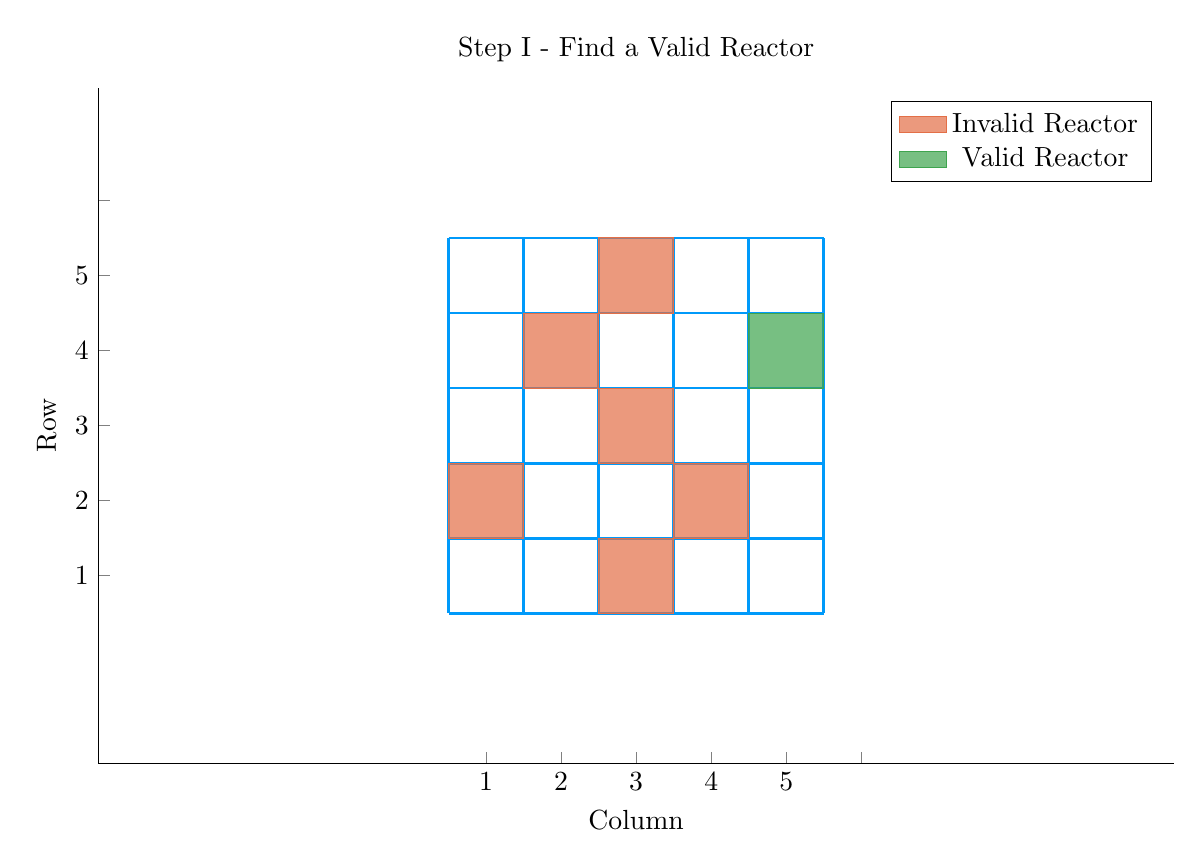
\begin{tikzpicture}[]
\begin{axis}[height = {101.6mm}, axis equal = {true}, ylabel = {Row}, title = {Step I - Find a Valid Reactor}, xmin = {0.0}, xmax = {5.0}, ymax = {7}, xlabel = {Column}, {unbounded coords=jump, xticklabel style={rotate = 0}, xmajorgrids = false, xtick = {0.5,1.5,2.5,3.5,4.5,5.5}, xticklabels = {1,2,3,4,5}, xtick align = inside, axis lines* = left, yticklabel style={rotate = 0}, ymajorgrids = false, ytick = {0.5,1.5,2.5,3.5,4.5,5.5}, yticklabels = {1,2,3,4,5}, ytick align = inside, axis lines* = left,     xshift = 0.0mm,
    yshift = 0.0mm,
    axis background/.style={fill={rgb,1:red,1.00000000;green,1.00000000;blue,1.00000000}}
}, ymin = {-2}, width = {152.4mm}]\addplot+ [color = {rgb,1:red,0.00000000;green,0.60560316;blue,0.97868012},
draw opacity=1.0,
line width=1,
solid,mark = none,
mark size = 2.0,
mark options = {
    color = {rgb,1:red,0.00000000;green,0.00000000;blue,0.00000000}, draw opacity = 1.0,
    fill = {rgb,1:red,0.00000000;green,0.60560316;blue,0.97868012}, fill opacity = 1.0,
    line width = 1,
    rotate = 0,
    solid
},forget plot]coordinates {
(0, 0)
(0, 5)
};
\addplot+ [color = {rgb,1:red,0.00000000;green,0.60560316;blue,0.97868012},
draw opacity=1.0,
line width=1,
solid,mark = none,
mark size = 2.0,
mark options = {
    color = {rgb,1:red,0.00000000;green,0.00000000;blue,0.00000000}, draw opacity = 1.0,
    fill = {rgb,1:red,0.00000000;green,0.60560316;blue,0.97868012}, fill opacity = 1.0,
    line width = 1,
    rotate = 0,
    solid
},forget plot]coordinates {
(0, 0)
(5, 0)
};
\addplot+ [color = {rgb,1:red,0.00000000;green,0.60560316;blue,0.97868012},
draw opacity=1.0,
line width=1,
solid,mark = none,
mark size = 2.0,
mark options = {
    color = {rgb,1:red,0.00000000;green,0.00000000;blue,0.00000000}, draw opacity = 1.0,
    fill = {rgb,1:red,0.00000000;green,0.60560316;blue,0.97868012}, fill opacity = 1.0,
    line width = 1,
    rotate = 0,
    solid
},forget plot]coordinates {
(1, 0)
(1, 5)
};
\addplot+ [color = {rgb,1:red,0.00000000;green,0.60560316;blue,0.97868012},
draw opacity=1.0,
line width=1,
solid,mark = none,
mark size = 2.0,
mark options = {
    color = {rgb,1:red,0.00000000;green,0.00000000;blue,0.00000000}, draw opacity = 1.0,
    fill = {rgb,1:red,0.00000000;green,0.60560316;blue,0.97868012}, fill opacity = 1.0,
    line width = 1,
    rotate = 0,
    solid
},forget plot]coordinates {
(0, 1)
(5, 1)
};
\addplot+ [color = {rgb,1:red,0.00000000;green,0.60560316;blue,0.97868012},
draw opacity=1.0,
line width=1,
solid,mark = none,
mark size = 2.0,
mark options = {
    color = {rgb,1:red,0.00000000;green,0.00000000;blue,0.00000000}, draw opacity = 1.0,
    fill = {rgb,1:red,0.00000000;green,0.60560316;blue,0.97868012}, fill opacity = 1.0,
    line width = 1,
    rotate = 0,
    solid
},forget plot]coordinates {
(2, 0)
(2, 5)
};
\addplot+ [color = {rgb,1:red,0.00000000;green,0.60560316;blue,0.97868012},
draw opacity=1.0,
line width=1,
solid,mark = none,
mark size = 2.0,
mark options = {
    color = {rgb,1:red,0.00000000;green,0.00000000;blue,0.00000000}, draw opacity = 1.0,
    fill = {rgb,1:red,0.00000000;green,0.60560316;blue,0.97868012}, fill opacity = 1.0,
    line width = 1,
    rotate = 0,
    solid
},forget plot]coordinates {
(0, 2)
(5, 2)
};
\addplot+ [color = {rgb,1:red,0.00000000;green,0.60560316;blue,0.97868012},
draw opacity=1.0,
line width=1,
solid,mark = none,
mark size = 2.0,
mark options = {
    color = {rgb,1:red,0.00000000;green,0.00000000;blue,0.00000000}, draw opacity = 1.0,
    fill = {rgb,1:red,0.00000000;green,0.60560316;blue,0.97868012}, fill opacity = 1.0,
    line width = 1,
    rotate = 0,
    solid
},forget plot]coordinates {
(3, 0)
(3, 5)
};
\addplot+ [color = {rgb,1:red,0.00000000;green,0.60560316;blue,0.97868012},
draw opacity=1.0,
line width=1,
solid,mark = none,
mark size = 2.0,
mark options = {
    color = {rgb,1:red,0.00000000;green,0.00000000;blue,0.00000000}, draw opacity = 1.0,
    fill = {rgb,1:red,0.00000000;green,0.60560316;blue,0.97868012}, fill opacity = 1.0,
    line width = 1,
    rotate = 0,
    solid
},forget plot]coordinates {
(0, 3)
(5, 3)
};
\addplot+ [color = {rgb,1:red,0.00000000;green,0.60560316;blue,0.97868012},
draw opacity=1.0,
line width=1,
solid,mark = none,
mark size = 2.0,
mark options = {
    color = {rgb,1:red,0.00000000;green,0.00000000;blue,0.00000000}, draw opacity = 1.0,
    fill = {rgb,1:red,0.00000000;green,0.60560316;blue,0.97868012}, fill opacity = 1.0,
    line width = 1,
    rotate = 0,
    solid
},forget plot]coordinates {
(4, 0)
(4, 5)
};
\addplot+ [color = {rgb,1:red,0.00000000;green,0.60560316;blue,0.97868012},
draw opacity=1.0,
line width=1,
solid,mark = none,
mark size = 2.0,
mark options = {
    color = {rgb,1:red,0.00000000;green,0.00000000;blue,0.00000000}, draw opacity = 1.0,
    fill = {rgb,1:red,0.00000000;green,0.60560316;blue,0.97868012}, fill opacity = 1.0,
    line width = 1,
    rotate = 0,
    solid
},forget plot]coordinates {
(0, 4)
(5, 4)
};
\addplot+ [color = {rgb,1:red,0.00000000;green,0.60560316;blue,0.97868012},
draw opacity=1.0,
line width=1,
solid,mark = none,
mark size = 2.0,
mark options = {
    color = {rgb,1:red,0.00000000;green,0.00000000;blue,0.00000000}, draw opacity = 1.0,
    fill = {rgb,1:red,0.00000000;green,0.60560316;blue,0.97868012}, fill opacity = 1.0,
    line width = 1,
    rotate = 0,
    solid
},forget plot]coordinates {
(5, 0)
(5, 5)
};
\addplot+ [color = {rgb,1:red,0.00000000;green,0.60560316;blue,0.97868012},
draw opacity=1.0,
line width=1,
solid,mark = none,
mark size = 2.0,
mark options = {
    color = {rgb,1:red,0.00000000;green,0.00000000;blue,0.00000000}, draw opacity = 1.0,
    fill = {rgb,1:red,0.00000000;green,0.60560316;blue,0.97868012}, fill opacity = 1.0,
    line width = 1,
    rotate = 0,
    solid
},forget plot]coordinates {
(0, 5)
(5, 5)
};
\addplot+ [color = {rgb,1:red,0.88887350;green,0.43564919;blue,0.27812294},
draw opacity=1.0,
line width=0,
solid,mark = none,
mark size = 2.0,
mark options = {
    color = {rgb,1:red,0.00000000;green,0.00000000;blue,0.00000000}, draw opacity = 1.0,
    fill = {rgb,1:red,0.88887350;green,0.43564919;blue,0.27812294}, fill opacity = 1.0,
    line width = 1,
    rotate = 0,
    solid
},fill = {rgb,1:red,0.88887350;green,0.43564919;blue,0.27812294}, fill opacity=0.7,area legend]coordinates {
(2, 2)
(2, 3)
(3, 3)
(3, 2)
(2, 2)
};
\addlegendentry{Invalid Reactor}
\addplot+ [color = {rgb,1:red,0.88887350;green,0.43564919;blue,0.27812294},
draw opacity=1.0,
line width=0,
solid,mark = none,
mark size = 2.0,
mark options = {
    color = {rgb,1:red,0.00000000;green,0.00000000;blue,0.00000000}, draw opacity = 1.0,
    fill = {rgb,1:red,0.88887350;green,0.43564919;blue,0.27812294}, fill opacity = 1.0,
    line width = 1,
    rotate = 0,
    solid
},fill = {rgb,1:red,0.88887350;green,0.43564919;blue,0.27812294}, fill opacity=0.7,forget plot]coordinates {
(1, 3)
(1, 4)
(2, 4)
(2, 3)
(1, 3)
};
\addplot+ [color = {rgb,1:red,0.88887350;green,0.43564919;blue,0.27812294},
draw opacity=1.0,
line width=0,
solid,mark = none,
mark size = 2.0,
mark options = {
    color = {rgb,1:red,0.00000000;green,0.00000000;blue,0.00000000}, draw opacity = 1.0,
    fill = {rgb,1:red,0.88887350;green,0.43564919;blue,0.27812294}, fill opacity = 1.0,
    line width = 1,
    rotate = 0,
    solid
},fill = {rgb,1:red,0.88887350;green,0.43564919;blue,0.27812294}, fill opacity=0.7,forget plot]coordinates {
(3, 1)
(3, 2)
(4, 2)
(4, 1)
(3, 1)
};
\addplot+ [color = {rgb,1:red,0.88887350;green,0.43564919;blue,0.27812294},
draw opacity=1.0,
line width=0,
solid,mark = none,
mark size = 2.0,
mark options = {
    color = {rgb,1:red,0.00000000;green,0.00000000;blue,0.00000000}, draw opacity = 1.0,
    fill = {rgb,1:red,0.88887350;green,0.43564919;blue,0.27812294}, fill opacity = 1.0,
    line width = 1,
    rotate = 0,
    solid
},fill = {rgb,1:red,0.88887350;green,0.43564919;blue,0.27812294}, fill opacity=0.7,forget plot]coordinates {
(2, 4)
(2, 5)
(3, 5)
(3, 4)
(2, 4)
};
\addplot+ [color = {rgb,1:red,0.88887350;green,0.43564919;blue,0.27812294},
draw opacity=1.0,
line width=0,
solid,mark = none,
mark size = 2.0,
mark options = {
    color = {rgb,1:red,0.00000000;green,0.00000000;blue,0.00000000}, draw opacity = 1.0,
    fill = {rgb,1:red,0.88887350;green,0.43564919;blue,0.27812294}, fill opacity = 1.0,
    line width = 1,
    rotate = 0,
    solid
},fill = {rgb,1:red,0.88887350;green,0.43564919;blue,0.27812294}, fill opacity=0.7,forget plot]coordinates {
(0, 1)
(0, 2)
(1, 2)
(1, 1)
(0, 1)
};
\addplot+ [color = {rgb,1:red,0.88887350;green,0.43564919;blue,0.27812294},
draw opacity=1.0,
line width=0,
solid,mark = none,
mark size = 2.0,
mark options = {
    color = {rgb,1:red,0.00000000;green,0.00000000;blue,0.00000000}, draw opacity = 1.0,
    fill = {rgb,1:red,0.88887350;green,0.43564919;blue,0.27812294}, fill opacity = 1.0,
    line width = 1,
    rotate = 0,
    solid
},fill = {rgb,1:red,0.88887350;green,0.43564919;blue,0.27812294}, fill opacity=0.7,forget plot]coordinates {
(2, 0)
(2, 1)
(3, 1)
(3, 0)
(2, 0)
};
\addplot+ [color = {rgb,1:red,0.24222430;green,0.64327509;blue,0.30444865},
draw opacity=1.0,
line width=0,
solid,mark = none,
mark size = 2.0,
mark options = {
    color = {rgb,1:red,0.00000000;green,0.00000000;blue,0.00000000}, draw opacity = 1.0,
    fill = {rgb,1:red,0.24222430;green,0.64327509;blue,0.30444865}, fill opacity = 1.0,
    line width = 1,
    rotate = 0,
    solid
},fill = {rgb,1:red,0.24222430;green,0.64327509;blue,0.30444865}, fill opacity=0.7,area legend]coordinates {
(4, 3)
(4, 4)
(5, 4)
(5, 3)
(4, 3)
};
\addlegendentry{Valid Reactor}
\end{axis}

\end{tikzpicture}

\end{adjustbox}
\caption{Minimize Cost Step I -- Find Valid Reactor}
\label{fig:step_one}
\end{figure}

After a valid reactor is found, its cost is recorded leading to a drill-down stage. In this step, the cost is continuously halved until a valid one cannot be found. Once this invalid reactor is reached, it sets a bound on the minimum cost reactor. As such, the final stage is a simple bisection step where the minimum cost is honed down to some acceptable margin of error -- see \cref{fig:minimize}.

\begin{figure*}
    \centering
    \begin{subfigure}[t]{0.8\textwidth}
        \centering
		\begin{adjustbox}{width=\textwidth}
			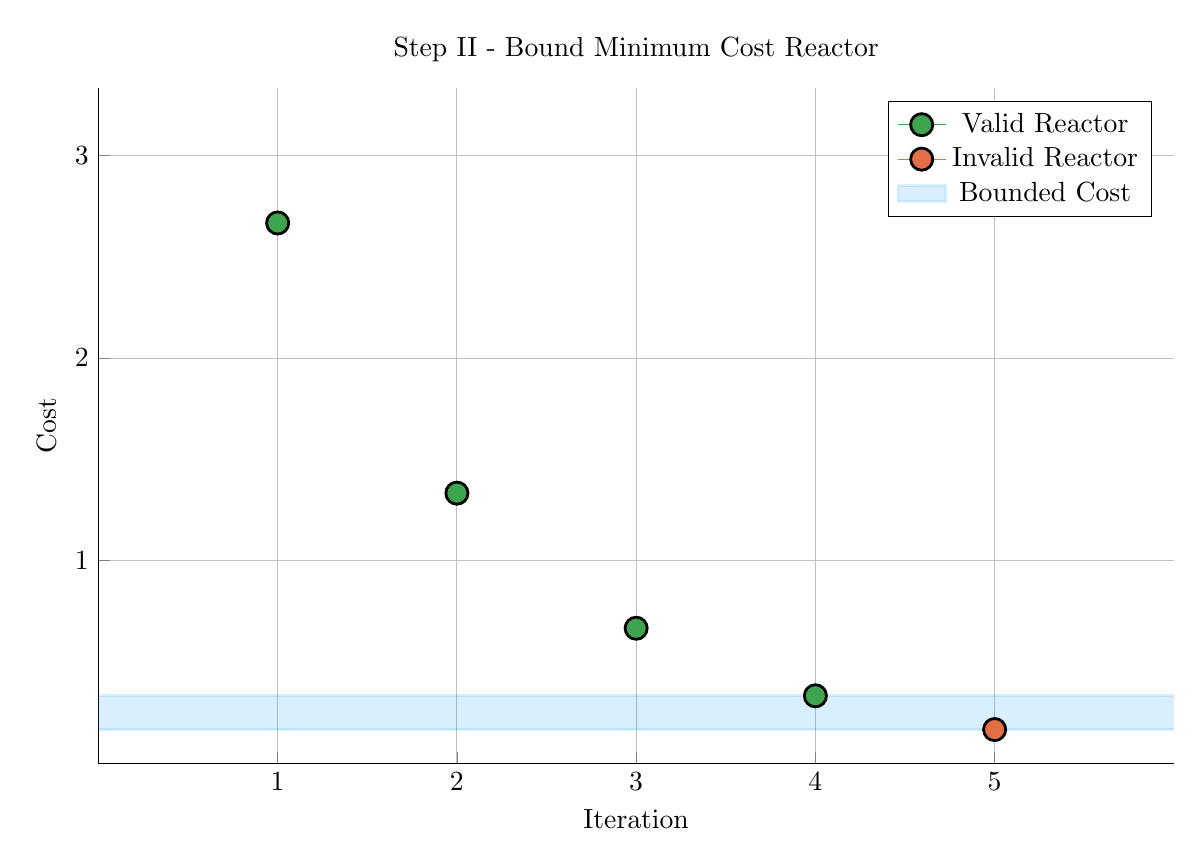
\begin{tikzpicture}[]
\begin{axis}[height = {101.6mm}, ylabel = {Cost}, title = {Step II - Bound Minimum Cost Reactor}, xmin = {0}, xmax = {6}, ymax = {40}, xlabel = {Iteration}, {unbounded coords=jump, xticklabel style={rotate = 0}, xmajorgrids = true, xtick = {1.0,2.0,3.0,4.0,5.0}, xticklabels = {1,2,3,4,5}, xtick align = inside, axis lines* = left, yticklabel style={rotate = 0}, ymajorgrids = true, ytick = {12,24,36}, yticklabels = {1,2,3}, ytick align = inside, axis lines* = left,     xshift = 0.0mm,
    yshift = 0.0mm,
    axis background/.style={fill={rgb,1:red,1.00000000;green,1.00000000;blue,1.00000000}}
}, ymin = {0}, width = {152.4mm}]\addplot+[draw=none, color = {rgb,1:red,0.24222430;green,0.64327509;blue,0.30444865},
draw opacity=1.0,
line width=0,
solid,mark = *,
mark size = 4.0,
mark options = {
    color = {rgb,1:red,0.00000000;green,0.00000000;blue,0.00000000}, draw opacity = 1.0,
    fill = {rgb,1:red,0.24222430;green,0.64327509;blue,0.30444865}, fill opacity = 1.0,
    line width = 1,
    rotate = 0,
    solid
}] coordinates {
(1.0, 32.0)
};
\addlegendentry{Valid Reactor}
\addplot+[draw=none, color = {rgb,1:red,0.24222430;green,0.64327509;blue,0.30444865},
draw opacity=1.0,
line width=0,
solid,mark = *,
mark size = 4.0,
mark options = {
    color = {rgb,1:red,0.00000000;green,0.00000000;blue,0.00000000}, draw opacity = 1.0,
    fill = {rgb,1:red,0.24222430;green,0.64327509;blue,0.30444865}, fill opacity = 1.0,
    line width = 1,
    rotate = 0,
    solid
},forget plot] coordinates {
(2.0, 16.0)
};
\addplot+[draw=none, color = {rgb,1:red,0.24222430;green,0.64327509;blue,0.30444865},
draw opacity=1.0,
line width=0,
solid,mark = *,
mark size = 4.0,
mark options = {
    color = {rgb,1:red,0.00000000;green,0.00000000;blue,0.00000000}, draw opacity = 1.0,
    fill = {rgb,1:red,0.24222430;green,0.64327509;blue,0.30444865}, fill opacity = 1.0,
    line width = 1,
    rotate = 0,
    solid
},forget plot] coordinates {
(3.0, 8.0)
};
\addplot+[draw=none, color = {rgb,1:red,0.24222430;green,0.64327509;blue,0.30444865},
draw opacity=1.0,
line width=0,
solid,mark = *,
mark size = 4.0,
mark options = {
    color = {rgb,1:red,0.00000000;green,0.00000000;blue,0.00000000}, draw opacity = 1.0,
    fill = {rgb,1:red,0.24222430;green,0.64327509;blue,0.30444865}, fill opacity = 1.0,
    line width = 1,
    rotate = 0,
    solid
},forget plot] coordinates {
(4.0, 4.0)
};
\addplot+[draw=none, color = {rgb,1:red,0.88887350;green,0.43564919;blue,0.27812294},
draw opacity=1.0,
line width=0,
solid,mark = *,
mark size = 4.0,
mark options = {
    color = {rgb,1:red,0.00000000;green,0.00000000;blue,0.00000000}, draw opacity = 1.0,
    fill = {rgb,1:red,0.88887350;green,0.43564919;blue,0.27812294}, fill opacity = 1.0,
    line width = 1,
    rotate = 0,
    solid
}] coordinates {
(5.0, 2.0)
};
\addlegendentry{Invalid Reactor}
\addplot+ [color = {rgb,1:red,0.00000000;green,0.60560316;blue,0.97868012},
draw opacity=0.15,
line width=1,
solid,mark = none,
mark size = 2.0,
mark options = {
    color = {rgb,1:red,0.00000000;green,0.00000000;blue,0.00000000}, draw opacity = 0.15,
    fill = {rgb,1:red,0.00000000;green,0.60560316;blue,0.97868012}, fill opacity = 0.15,
    line width = 1,
    rotate = 0,
    solid
},fill = {rgb,1:red,0.00000000;green,0.60560316;blue,0.97868012}, fill opacity=0.15,area legend]coordinates {
(-1.0, 4.0)
(-1.0, 2.0)
(7.0, 2.0)
(7.0, 4.0)
(-1.0, 4.0)
};
\addlegendentry{Bounded Cost}
\end{axis}

\end{tikzpicture}

		\end{adjustbox}
        \caption{ Minimize Step II }
    \end{subfigure} 
    \par \bigskip \par \bigskip 
    \begin{subfigure}[t]{0.8\textwidth}
        \centering
		\begin{adjustbox}{width=\textwidth}
			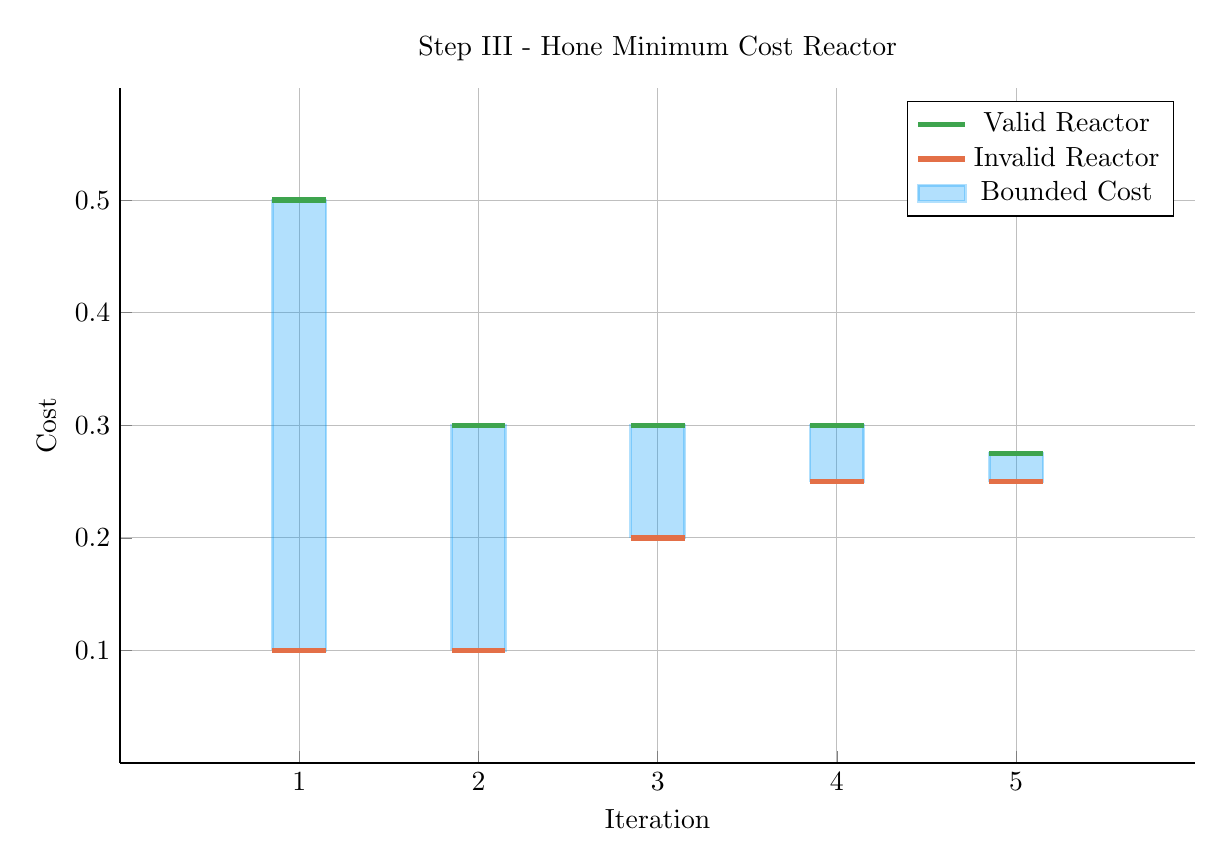
\begin{tikzpicture}[]
\begin{axis}[height = {101.6mm}, ylabel = {Cost}, title = {Step III - Hone Minimum Cost Reactor}, xmin = {0}, xmax = {6}, ymax = {0.6}, xlabel = {Iteration}, {unbounded coords=jump, xticklabel style={rotate = 0}, xmajorgrids = true, xtick = {1.0,2.0,3.0,4.0,5.0}, xticklabels = {1,2,3,4,5}, xtick align = inside, axis lines* = left, yticklabel style={rotate = 0}, ymajorgrids = true, ytick = {0.1,0.2,0.3,0.4,0.5}, yticklabels = {0.1,0.2,0.3,0.4,0.5}, ytick align = inside, axis lines* = left,     xshift = 0.0mm,
    yshift = 0.0mm,
    axis background/.style={fill={rgb,1:red,1.00000000;green,1.00000000;blue,1.00000000}}
}, ymin = {0}, width = {152.4mm}]\addplot+ [color = {rgb,1:red,0.00000000;green,0.60560316;blue,0.97868012},
draw opacity=0.3,
line width=1,
solid,mark = none,
mark size = 2.0,
mark options = {
    color = {rgb,1:red,0.00000000;green,0.00000000;blue,0.00000000}, draw opacity = 0.3,
    fill = {rgb,1:red,0.00000000;green,0.60560316;blue,0.97868012}, fill opacity = 0.3,
    line width = 1,
    rotate = 0,
    solid
},fill = {rgb,1:red,0.00000000;green,0.60560316;blue,0.97868012}, fill opacity=0.3,forget plot]coordinates {
(0.85, 0.1)
(0.85, 0.5)
(1.15, 0.5)
(1.15, 0.1)
(0.85, 0.1)
};
\addplot+ [color = {rgb,1:red,0.24222430;green,0.64327509;blue,0.30444865},
draw opacity=1.0,
line width=2,
solid,mark = none,
mark size = 2.0,
mark options = {
    color = {rgb,1:red,0.00000000;green,0.00000000;blue,0.00000000}, draw opacity = 1.0,
    fill = {rgb,1:red,0.24222430;green,0.64327509;blue,0.30444865}, fill opacity = 1.0,
    line width = 1,
    rotate = 0,
    solid
}]coordinates {
(0.85, 0.5)
(1.15, 0.5)
};
\addlegendentry{Valid Reactor}
\addplot+ [color = {rgb,1:red,0.88887350;green,0.43564919;blue,0.27812294},
draw opacity=1.0,
line width=2,
solid,mark = none,
mark size = 2.0,
mark options = {
    color = {rgb,1:red,0.00000000;green,0.00000000;blue,0.00000000}, draw opacity = 1.0,
    fill = {rgb,1:red,0.88887350;green,0.43564919;blue,0.27812294}, fill opacity = 1.0,
    line width = 1,
    rotate = 0,
    solid
}]coordinates {
(0.85, 0.1)
(1.15, 0.1)
};
\addlegendentry{Invalid Reactor}
\addplot+ [color = {rgb,1:red,0.00000000;green,0.60560316;blue,0.97868012},
draw opacity=0.3,
line width=1,
solid,mark = none,
mark size = 2.0,
mark options = {
    color = {rgb,1:red,0.00000000;green,0.00000000;blue,0.00000000}, draw opacity = 0.3,
    fill = {rgb,1:red,0.00000000;green,0.60560316;blue,0.97868012}, fill opacity = 0.3,
    line width = 1,
    rotate = 0,
    solid
},fill = {rgb,1:red,0.00000000;green,0.60560316;blue,0.97868012}, fill opacity=0.3,area legend]coordinates {
(1.85, 0.1)
(1.85, 0.3)
(2.15, 0.3)
(2.15, 0.1)
(1.85, 0.1)
};
\addlegendentry{Bounded Cost}
\addplot+ [color = {rgb,1:red,0.88887350;green,0.43564919;blue,0.27812294},
draw opacity=1.0,
line width=2,
solid,mark = none,
mark size = 2.0,
mark options = {
    color = {rgb,1:red,0.00000000;green,0.00000000;blue,0.00000000}, draw opacity = 1.0,
    fill = {rgb,1:red,0.88887350;green,0.43564919;blue,0.27812294}, fill opacity = 1.0,
    line width = 1,
    rotate = 0,
    solid
},forget plot]coordinates {
(1.85, 0.1)
(2.15, 0.1)
};
\addplot+ [color = {rgb,1:red,0.24222430;green,0.64327509;blue,0.30444865},
draw opacity=1.0,
line width=2,
solid,mark = none,
mark size = 2.0,
mark options = {
    color = {rgb,1:red,0.00000000;green,0.00000000;blue,0.00000000}, draw opacity = 1.0,
    fill = {rgb,1:red,0.24222430;green,0.64327509;blue,0.30444865}, fill opacity = 1.0,
    line width = 1,
    rotate = 0,
    solid
},forget plot]coordinates {
(1.85, 0.3)
(2.15, 0.3)
};
\addplot+ [color = {rgb,1:red,0.00000000;green,0.60560316;blue,0.97868012},
draw opacity=0.3,
line width=1,
solid,mark = none,
mark size = 2.0,
mark options = {
    color = {rgb,1:red,0.00000000;green,0.00000000;blue,0.00000000}, draw opacity = 0.3,
    fill = {rgb,1:red,0.00000000;green,0.60560316;blue,0.97868012}, fill opacity = 0.3,
    line width = 1,
    rotate = 0,
    solid
},fill = {rgb,1:red,0.00000000;green,0.60560316;blue,0.97868012}, fill opacity=0.3,forget plot]coordinates {
(2.85, 0.2)
(2.85, 0.3)
(3.15, 0.3)
(3.15, 0.2)
(2.85, 0.2)
};
\addplot+ [color = {rgb,1:red,0.88887350;green,0.43564919;blue,0.27812294},
draw opacity=1.0,
line width=2,
solid,mark = none,
mark size = 2.0,
mark options = {
    color = {rgb,1:red,0.00000000;green,0.00000000;blue,0.00000000}, draw opacity = 1.0,
    fill = {rgb,1:red,0.88887350;green,0.43564919;blue,0.27812294}, fill opacity = 1.0,
    line width = 1,
    rotate = 0,
    solid
},forget plot]coordinates {
(2.85, 0.2)
(3.15, 0.2)
};
\addplot+ [color = {rgb,1:red,0.24222430;green,0.64327509;blue,0.30444865},
draw opacity=1.0,
line width=2,
solid,mark = none,
mark size = 2.0,
mark options = {
    color = {rgb,1:red,0.00000000;green,0.00000000;blue,0.00000000}, draw opacity = 1.0,
    fill = {rgb,1:red,0.24222430;green,0.64327509;blue,0.30444865}, fill opacity = 1.0,
    line width = 1,
    rotate = 0,
    solid
},forget plot]coordinates {
(2.85, 0.3)
(3.15, 0.3)
};
\addplot+ [color = {rgb,1:red,0.00000000;green,0.60560316;blue,0.97868012},
draw opacity=0.3,
line width=1,
solid,mark = none,
mark size = 2.0,
mark options = {
    color = {rgb,1:red,0.00000000;green,0.00000000;blue,0.00000000}, draw opacity = 0.3,
    fill = {rgb,1:red,0.00000000;green,0.60560316;blue,0.97868012}, fill opacity = 0.3,
    line width = 1,
    rotate = 0,
    solid
},fill = {rgb,1:red,0.00000000;green,0.60560316;blue,0.97868012}, fill opacity=0.3,forget plot]coordinates {
(3.85, 0.25)
(3.85, 0.3)
(4.15, 0.3)
(4.15, 0.25)
(3.85, 0.25)
};
\addplot+ [color = {rgb,1:red,0.88887350;green,0.43564919;blue,0.27812294},
draw opacity=1.0,
line width=2,
solid,mark = none,
mark size = 2.0,
mark options = {
    color = {rgb,1:red,0.00000000;green,0.00000000;blue,0.00000000}, draw opacity = 1.0,
    fill = {rgb,1:red,0.88887350;green,0.43564919;blue,0.27812294}, fill opacity = 1.0,
    line width = 1,
    rotate = 0,
    solid
},forget plot]coordinates {
(3.85, 0.25)
(4.15, 0.25)
};
\addplot+ [color = {rgb,1:red,0.24222430;green,0.64327509;blue,0.30444865},
draw opacity=1.0,
line width=2,
solid,mark = none,
mark size = 2.0,
mark options = {
    color = {rgb,1:red,0.00000000;green,0.00000000;blue,0.00000000}, draw opacity = 1.0,
    fill = {rgb,1:red,0.24222430;green,0.64327509;blue,0.30444865}, fill opacity = 1.0,
    line width = 1,
    rotate = 0,
    solid
},forget plot]coordinates {
(3.85, 0.3)
(4.15, 0.3)
};
\addplot+ [color = {rgb,1:red,0.00000000;green,0.60560316;blue,0.97868012},
draw opacity=0.3,
line width=1,
solid,mark = none,
mark size = 2.0,
mark options = {
    color = {rgb,1:red,0.00000000;green,0.00000000;blue,0.00000000}, draw opacity = 0.3,
    fill = {rgb,1:red,0.00000000;green,0.60560316;blue,0.97868012}, fill opacity = 0.3,
    line width = 1,
    rotate = 0,
    solid
},fill = {rgb,1:red,0.00000000;green,0.60560316;blue,0.97868012}, fill opacity=0.3,forget plot]coordinates {
(4.85, 0.25)
(4.85, 0.275)
(5.15, 0.275)
(5.15, 0.25)
(4.85, 0.25)
};
\addplot+ [color = {rgb,1:red,0.88887350;green,0.43564919;blue,0.27812294},
draw opacity=1.0,
line width=2,
solid,mark = none,
mark size = 2.0,
mark options = {
    color = {rgb,1:red,0.00000000;green,0.00000000;blue,0.00000000}, draw opacity = 1.0,
    fill = {rgb,1:red,0.88887350;green,0.43564919;blue,0.27812294}, fill opacity = 1.0,
    line width = 1,
    rotate = 0,
    solid
},forget plot]coordinates {
(4.85, 0.25)
(5.15, 0.25)
};
\addplot+ [color = {rgb,1:red,0.24222430;green,0.64327509;blue,0.30444865},
draw opacity=1.0,
line width=2,
solid,mark = none,
mark size = 2.0,
mark options = {
    color = {rgb,1:red,0.00000000;green,0.00000000;blue,0.00000000}, draw opacity = 1.0,
    fill = {rgb,1:red,0.24222430;green,0.64327509;blue,0.30444865}, fill opacity = 1.0,
    line width = 1,
    rotate = 0,
    solid
},forget plot]coordinates {
(4.85, 0.275)
(5.15, 0.275)
};
\end{axis}

\end{tikzpicture}

		\end{adjustbox}
        \caption{ Minimize Step III }
    \end{subfigure}
    \par \bigskip \par \bigskip    
    \caption{Minimize Cost Step II/III -- Optimize Reactor}
    \label{fig:minimize} 
\end{figure*}

\subsection{Pinning Floating Variables} 

The remaining collection of closure equations is for the five floating variables in the systems model: $R_0$, $B_0$, $\overline n$, $\overline T$, and $I_P$. As we are making equations of the following form, the formulas for $R_0$, $B_0$, and $I_P$ are trivial.

\begin{equation}
	\tag{\ref{eq:rbi}}
	R_0^{\, \gamma_R} \cdot B_0^{\, \gamma_B} \cdot I_P^{\, \gamma_I} = G( \overline T )
\end{equation}

Next, the equation for $\overline n$ -- shown in \cref{table:eq} -- is just a simple undoing of the Greenwald density limit. The remaining equation is then from the original temperature equation:

\begin{equation}
	\tag{\ref{eq:tbar}}
	\overline T = const.
\end{equation}

As was assumed earlier, this is sort of a default equation for the systems model. By this, we mean reactor curves can be created by scanning over temperatures, i.e. set $\overline T = 5 \ \textnormal{keV}$ in one run, 10 in the next, etc. This temperature equation also brings up a subtlety of the model, as it does not depend on current, radius, or magnet strength.

The algorithm that motivated this generalized equation approach most notably bifurcates in the situation where the closure equation does not depend on $R_0$, $B_0$, or $I_P$ (i.e. the temperature equation). The two scenarios are given in \cref{eq:case_1_R,eq:case_1_B,eq:case_1_I,eq:case_1_gamma,eq:case_2_R,eq:case_2_B,eq:case_2_gamma} -- where at least $R_0$ and $B_0$ are substituted out of the system. In the temperature case, $I_P$ is not needed to be explicitly removed. 

Concretely, the root solve for the temperature  scenario is for the current, whereas it is for the temperature in all other cases. The nomenclature in the code is a \emph{match} for Scenario I (i.e. root solving for plasma temperature), and a \emph{solve} for Scenario II (i.e. root solving for plasma current).

\subsubsection{Scenario I -- Match for $\overline T$}

\begin{equation}
	\label{eq:case_1_R}
	R_0( \overline T) = \left( 
	G_1 ^ {  \, ( \gamma_{B,2} \, \gamma_{I,3} - \gamma_{B,3} \, \gamma_{I,2} ) } \cdot 
	G_2 ^ {  \, ( \gamma_{B,3} \, \gamma_{I,1} - \gamma_{B,1} \, \gamma_{I,3} ) } \cdot 
	G_3 ^ {  \, ( \gamma_{B,1} \, \gamma_{I,2} - \gamma_{B,2} \, \gamma_{I,1} ) }\right)^{ \frac{1}{\gamma_{RBI}} }
\end{equation}

\begin{equation}
	\label{eq:case_1_B}
	B_0( \overline T) = \left( 
	G_1 ^ {  \, ( \gamma_{I,2} \, \gamma_{R,3} - \gamma_{I,3} \, \gamma_{R,2} ) } \cdot 
	G_2 ^ {  \, ( \gamma_{I,3} \, \gamma_{R,1} - \gamma_{I,1} \, \gamma_{R,3} ) } \cdot 
	G_3 ^ {  \, ( \gamma_{I,1} \, \gamma_{R,2} - \gamma_{I,2} \, \gamma_{R,1} ) }\right)^{ \frac{1}{\gamma_{RBI}} }
\end{equation}

\begin{equation}
	\label{eq:case_1_I}
	I_P( \overline T) = \left( 
	G_1 ^ {  \, ( \gamma_{R,2} \, \gamma_{B,3} - \gamma_{R,3} \, \gamma_{B,2} ) } \cdot 
	G_2 ^ {  \, ( \gamma_{R,3} \, \gamma_{B,1} - \gamma_{R,1} \, \gamma_{B,3} ) } \cdot 
	G_3 ^ {  \, ( \gamma_{R,1} \, \gamma_{B,2} - \gamma_{R,2} \, \gamma_{B,1} ) }\right)^{ \frac{1}{\gamma_{RBI}} }
\end{equation}

\begin{gather}
	\label{eq:case_1_gamma}
	\gamma_{RBI} = ( \gamma_{R,1} \, \gamma_{B,2} \, \gamma_{I,3} +  \gamma_{R,2} \, \gamma_{B,3} \, \gamma_{I,1} + \gamma_{R,3} \, \gamma_{B,1} \, \gamma_{I,2} ) - \\
	\ \ \ \ \ \ \ \ \ \ \ \ \ \ \ ( \gamma_{R,1} \, \gamma_{B,3} \, \gamma_{I,2} +  \gamma_{R,2} \, \gamma_{B,1} \, \gamma_{I,3} + \gamma_{R,3} \, \gamma_{B,2} \, \gamma_{I,1} ) \nonumber
\end{gather}

\subsubsection{Scenario II -- Solve for $I_P$}

\begin{equation}
	\label{eq:case_2_R}
	R_0( \overline T) = \left( 
	G_1 ^ {  \, \gamma_{B,2} } \cdot 
	G_2 ^ {  \, -\gamma_{B,1} } \cdot 
	I_P ^ {  \, ( \gamma_{B,1} \, \gamma_{I,2} - \gamma_{B,2} \, \gamma_{I,1} ) }\right)^{ \frac{1}{\gamma_{RBT}} }
\end{equation}

\begin{equation}
	\label{eq:case_2_B}
	B_0( \overline T) = \left( 
	G_1 ^ {  \, -\gamma_{R,2} } \cdot 
	G_2 ^ {  \, \gamma_{R,1} } \cdot 
	I_P ^ {  \, ( \gamma_{I,1} \, \gamma_{R,2} - \gamma_{I,2} \, \gamma_{R,1} ) }\right)^{ \frac{1}{\gamma_{RBT}} }
\end{equation}

\begin{equation}
	\label{eq:case_2_gamma}
	\gamma_{RBT} = \gamma_{R,1} \, \gamma_{B,2} - \gamma_{R,2} \, \gamma_{B,1}
\end{equation}

\section{Wrapping up the Logic} 

As stated at the beginning of the chapter, this systems model basically boils down to a simple 5 equation/5 unknown algebra problem. The Greenwald density was implicitly used in the initial derive to simplify the logic. The current balance was then delegated to be the root solve equation. Lastly, three equations were needed to remove the major radius and magnet strength, as well as either the current or temperature. These 16 equations were given in \cref{table:eq} with the generalized solution given in \cref{eq:case_1_R,eq:case_1_B,eq:case_1_I,eq:case_1_gamma,eq:case_2_R,eq:case_2_B,eq:case_2_gamma}.

This now sets the stage for the most interesting part of the document -- the results. In true Dickens fashion, they will come in several forms. The first result type we will encounter will be temperature scans. These allow us to validate the model by comparing it to several designs from the literature. These will use the Scenario II solver.

Moving onto examples of the Scenario I solver are sensitivity studies and Monte Carlo samplings. The simple one variable sensitivities will reveal local trends from sweeping various fixed (i.e. input) variables -- namely H, $\kappa$, $B_{CS}$, etc. Whereas the samplings will highlight global trends as many fixed/input variables are allowed to vary simultaneously.

 These Scenario I flavors are further subdivided in regards to the nature of their closure equation. The first flavor comes from finding so called two limit solutions, which live at the point where the beta and kink (or wall) limits are just marginally satisfied. The second main type is then minimum cost reactors -- measured in either capital cost or cost-per-watt. These will be used in depth next chapter.
 
%\end{document}

%\documentclass[11pt]{book}
%
%\setlength{\parindent}{0pt}
%\setlength{\parskip}{8pt}
%
%\usepackage{amsmath}
%\usepackage{amssymb}
%\usepackage{hyperref}
%\usepackage{cleveref}
%
%\renewcommand*{\thefootnote}{\fnsymbol{footnote}}
%
%\setcounter{chapter}{3}
%
%\begin{document}
%
%\section*{A Levelized Comparison of \\ Pulsed and Steady-State Tokamaks}
%
%\let\cleardoublepage\relax \tableofcontents \newpage

\chapter{Presenting the Code Results}

\section{Validating Code with other Models}

\newpage 

\subsection{Comparing with the PSFC Arc Reactor}

\begin{figure*}[h!]
    \centering
    \hfill 
    \begin{subfigure}[t]{0.45\textwidth}
        \centering
    \begin{adjustbox}{width=\textwidth}
      \Large
      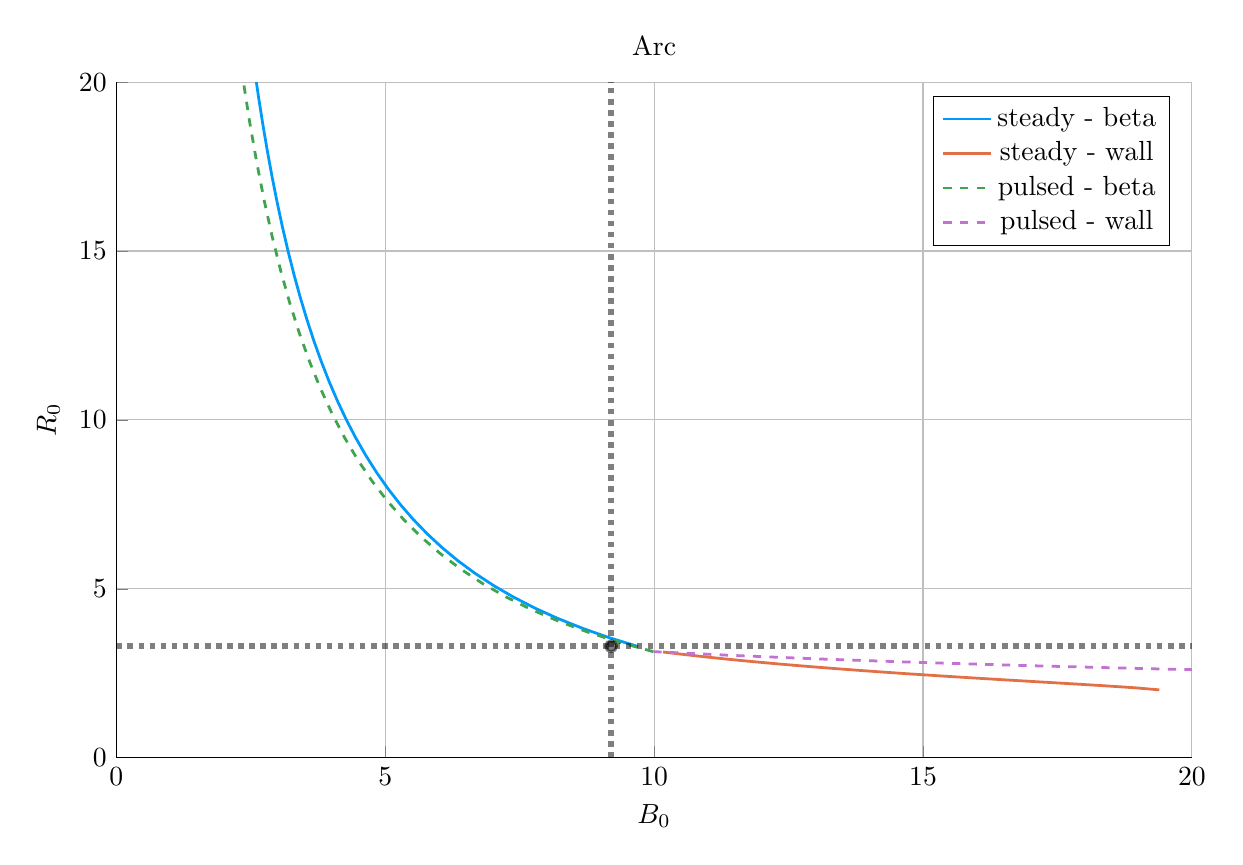
\begin{tikzpicture}[]
\begin{axis}[height = {101.6mm}, ylabel = {$R_0$}, title = {Arc}, xmin = {0.0}, xmax = {20.0}, ymax = {20.0}, xlabel = {$B_0$}, {unbounded coords=jump, scaled x ticks = false, xticklabel style={rotate = 0}, xmajorgrids = true, xtick = {0.0,5.0,10.0,15.0,20.0}, xticklabels = {0,5,10,15,20}, xtick align = inside, axis lines* = left, scaled y ticks = false, yticklabel style={rotate = 0}, ymajorgrids = true, ytick = {0.0,5.0,10.0,15.0,20.0}, yticklabels = {0,5,10,15,20}, ytick align = inside, axis lines* = left,     xshift = 0.0mm,
    yshift = 0.0mm,
    axis background/.style={fill={rgb,1:red,1.00000000;green,1.00000000;blue,1.00000000}}
}, ymin = {0.0}, width = {152.4mm}]\addplot+ [color = {rgb,1:red,0.00000000;green,0.60560316;blue,0.97868012},
draw opacity=1.0,
line width=1,
solid,mark = none,
mark size = 2.0,
mark options = {
    color = {rgb,1:red,0.00000000;green,0.00000000;blue,0.00000000}, draw opacity = 1.0,
    fill = {rgb,1:red,0.00000000;green,0.60560316;blue,0.97868012}, fill opacity = 1.0,
    line width = 1,
    rotate = 0,
    solid
}]coordinates {
(9.701206080853105, 3.2904233285656006)
(9.162315904693079, 3.553631706046861)
(8.664301107137337, 3.8315748016260343)
(8.203576462497304, 4.124583886864978)
(7.776718537485166, 4.433072975674755)
(7.380720231870917, 4.75741949036414)
(7.012886014999712, 5.097987291342331)
(6.670795005901889, 5.4551257000070565)
(6.352268997292712, 5.829168567645448)
(6.055344682097163, 6.220433393277178)
(5.778249464564785, 6.629220493040615)
(5.519380338856715, 7.05581222339423)
(5.2772854007125325, 7.500472260074458)
(5.050647625972996, 7.963444934423652)
(4.838270606140816, 8.444954628380609)
(4.639065978019038, 8.94520522910952)
(4.4520423235376105, 9.464379643936518)
(4.276295348572609, 10.002639375969222)
(4.110999177018484, 10.56012416048812)
(3.9553986195015125, 11.136951661929974)
(3.8088022956698633, 11.733217231026282)
(3.6705765055641186, 12.34899372141899)
(3.54013975965751, 12.984331364849716)
(3.4169578891619192, 13.639257703809928)
(3.30053966845824, 14.313777580345645)
(3.1904328903033052, 15.007873179535935)
(3.086220842019516, 15.721504126002731)
(2.9875191373772063, 16.45460763166718)
(2.8939728644914635, 17.207098692842226)
(2.8052540149097247, 17.97887033463821)
(2.7210591632720242, 18.7697939005645)
(2.6411073705789065, 19.579719385129263)
(2.565138287279709, 20.40847580717446)
(2.492910435164382, 21.255871621630877)
(2.4241996494611984, 22.12169516733927)
(2.3587976646588236, 23.0057151485579)
(2.296510829425685, 23.907681147764652)
(2.237158937627476, 24.827324167354146)
(2.180574163874242, 25.764357197843207)
(2.126600093288366, 26.71847581021091)
(2.075090836295778, 27.689358770027713)
(2.0259102202234582, 28.676668671060817)
(1.978931050353818, 29.68005258608471)
(1.9340344338545452, 30.69914273267572)
(1.8911091606836798, 31.733557151818793)
(1.8500511361739687, 32.78290039722107)
(1.8107628605384507, 33.846764233283025)
(1.773152951016952, 34.92472833975579)
(1.7371357028100902, 36.01636102117257)
(1.7026306853269466, 37.121219919229354)
(1.6695623706125668, 38.23885272635799)
(1.6378597911249178, 39.368797898817405)
(1.607456224302725, 40.51058536770822)
(1.5782889016090462, 41.663737246396295)
(1.5502987399539199, 42.82776853291479)
(1.5234300935954943, 44.00218780599217)
(1.4976305247952577, 45.18649791343829)
(1.4728505916614916, 46.38019665170201)
(1.4490436517578602, 47.58277743549339)
(1.4261656801829077, 48.79372995643627)
};
\addlegendentry{steady - beta}
\addplot+ [color = {rgb,1:red,0.88887350;green,0.43564919;blue,0.27812294},
draw opacity=1.0,
line width=1,
solid,mark = none,
mark size = 2.0,
mark options = {
    color = {rgb,1:red,0.00000000;green,0.00000000;blue,0.00000000}, draw opacity = 1.0,
    fill = {rgb,1:red,0.88887350;green,0.43564919;blue,0.27812294}, fill opacity = 1.0,
    line width = 1,
    rotate = 0,
    solid
}]coordinates {
(19.394007482712425, 2.006855814841082)
(18.932196567189358, 2.070220226465634)
(18.296989378345195, 2.1362327099649083)
(17.587029315408756, 2.2039322514902886)
(16.847882407994106, 2.272885741349308)
(16.111374502564406, 2.3427307443133163)
(15.396027314547156, 2.4132115621474344)
(14.710952688793137, 2.484165095168367)
(14.06168447794857, 2.555449485048069)
(13.450465418483889, 2.6269568263788754)
(12.877644538645335, 2.6986005527245354)
(12.342394470642008, 2.7703103261458715)
(11.843182246608265, 2.8420284550528074)
(11.376441269625893, 2.9137564749008216)
(10.944966372727551, 2.985307257194073)
(10.541663878705513, 3.056795384934831)
(10.165908182236457, 3.128148092221394)
};
\addlegendentry{steady - wall}
\addplot+ [color = {rgb,1:red,0.24222430;green,0.64327509;blue,0.30444865},
draw opacity=1.0,
line width=1,
dashed,mark = none,
mark size = 2.0,
mark options = {
    color = {rgb,1:red,0.00000000;green,0.00000000;blue,0.00000000}, draw opacity = 1.0,
    fill = {rgb,1:red,0.24222430;green,0.64327509;blue,0.30444865}, fill opacity = 1.0,
    line width = 1,
    rotate = 0,
    solid
}]coordinates {
(9.980483622051658, 3.1402982942956537)
(9.392786903460065, 3.3984668375583613)
(8.79273598103983, 3.7029994270206985)
(8.23820290909994, 4.029752381934837)
(7.725182218401588, 4.380005330007902)
(7.250078106370205, 4.755088191072525)
(6.80965553466646, 5.15638156809462)
(6.400998063035608, 5.585317075247801)
(6.0214713600430425, 6.043377623224966)
(5.668691517461799, 6.532097691007738)
(5.340497445229901, 7.053063624618788)
(5.034926745580058, 7.607914017422467)
(4.750194564008521, 8.198340243900201)
(4.484674995755211, 8.826087240213646)
(4.236884692979903, 9.49295465115087)
(4.00546837264544, 10.200798495308337)
(3.7891859704718387, 10.951533539957822)
(3.5869012239550364, 11.747136625739826)
(3.3975714987448393, 12.589651241396528)
(3.2202386987489797, 13.481193723261853)
(3.0540211220494466, 14.423961547290066)
(2.8981061427709687, 15.420244298711943)
(2.7517436139566023, 16.472438053930638)
(2.6142398986781377, 17.58306410230943)
(2.4849524463010138, 18.754793188384546)
(2.363284838174807, 19.990476791576892)
(2.248682232019848, 21.293187416028662)
(2.140627136740878, 22.666270490916787)
(2.038635448877246, 24.113411362836906)
(1.9422526775794744, 25.638722123308433)
(1.8510502754751532, 27.246854857488287)
(1.7646219756564088, 28.94315065234289)
(1.6825800061969869, 30.73383791051506)
(1.6045510059627948, 32.62630011975996)
(1.53017138625397, 34.629443897654504)
(1.4590817483192686, 36.754215952550474)
(1.3909197311384796, 39.01434852880224)
(1.3253102336217724, 41.42746903285954)
(1.261851128383913, 44.01681696754988)
(1.20009089049112, 46.81403058684408)
(1.1394908096975784, 49.863950342519615)
};
\addlegendentry{pulsed - beta}
\addplot+ [color = {rgb,1:red,0.76444018;green,0.44411178;blue,0.82429754},
draw opacity=1.0,
line width=1,
dashed,mark = none,
mark size = 2.0,
mark options = {
    color = {rgb,1:red,0.00000000;green,0.00000000;blue,0.00000000}, draw opacity = 1.0,
    fill = {rgb,1:red,0.76444018;green,0.44411178;blue,0.82429754}, fill opacity = 1.0,
    line width = 1,
    rotate = 0,
    solid
}]coordinates {
(29.27715761652869, 2.3448804182939873)
(25.4410619834368, 2.4377937236066716)
(22.158819835998365, 2.5322208586485804)
(19.342453256965573, 2.628163744265164)
(16.919364280634177, 2.7256238396687067)
(14.829378672669455, 2.8246020951898183)
(13.022412368922526, 2.9250989082568273)
(11.456617692058645, 3.0271140820266207)
(10.096901921254785, 3.1306467862637533)
(9.980483622051658, 3.1402982942956537)
};
\addlegendentry{pulsed - wall}
\addplot+ [color = {rgb,1:red,0.00000000;green,0.00000000;blue,0.00000000},
draw opacity=0.5,
line width=2,
dotted,mark = none,
mark size = 2.0,
mark options = {
    color = {rgb,1:red,0.00000000;green,0.00000000;blue,0.00000000}, draw opacity = 0.5,
    fill = {rgb,1:red,0.00000000;green,0.00000000;blue,0.00000000}, fill opacity = 0.5,
    line width = 1,
    rotate = 0,
    solid
},forget plot]coordinates {
(0.0, 3.3)
(20.0, 3.3)
};
\addplot+ [color = {rgb,1:red,0.00000000;green,0.00000000;blue,0.00000000},
draw opacity=0.5,
line width=2,
dotted,mark = none,
mark size = 2.0,
mark options = {
    color = {rgb,1:red,0.00000000;green,0.00000000;blue,0.00000000}, draw opacity = 0.5,
    fill = {rgb,1:red,0.00000000;green,0.00000000;blue,0.00000000}, fill opacity = 0.5,
    line width = 1,
    rotate = 0,
    solid
},forget plot]coordinates {
(9.2, 0.0)
(9.2, 20.0)
};
\addplot+[draw=none, color = {rgb,1:red,0.00000000;green,0.00000000;blue,0.00000000},
draw opacity=0.5,
line width=0,
solid,mark = *,
mark size = 2.0,
mark options = {
    color = {rgb,1:red,0.00000000;green,0.00000000;blue,0.00000000}, draw opacity = 0.5,
    fill = {rgb,1:red,0.00000000;green,0.00000000;blue,0.00000000}, fill opacity = 0.5,
    line width = 1,
    rotate = 0,
    solid
},forget plot] coordinates {
(9.2, 3.3)
};
\end{axis}

\end{tikzpicture}

    \end{adjustbox}
        \caption{$R_0$ vs $B_0$}
    \end{subfigure}
    \hfill
    \begin{subfigure}[t]{0.45\textwidth}
        \centering
    \begin{adjustbox}{width=\textwidth}
      \Large
      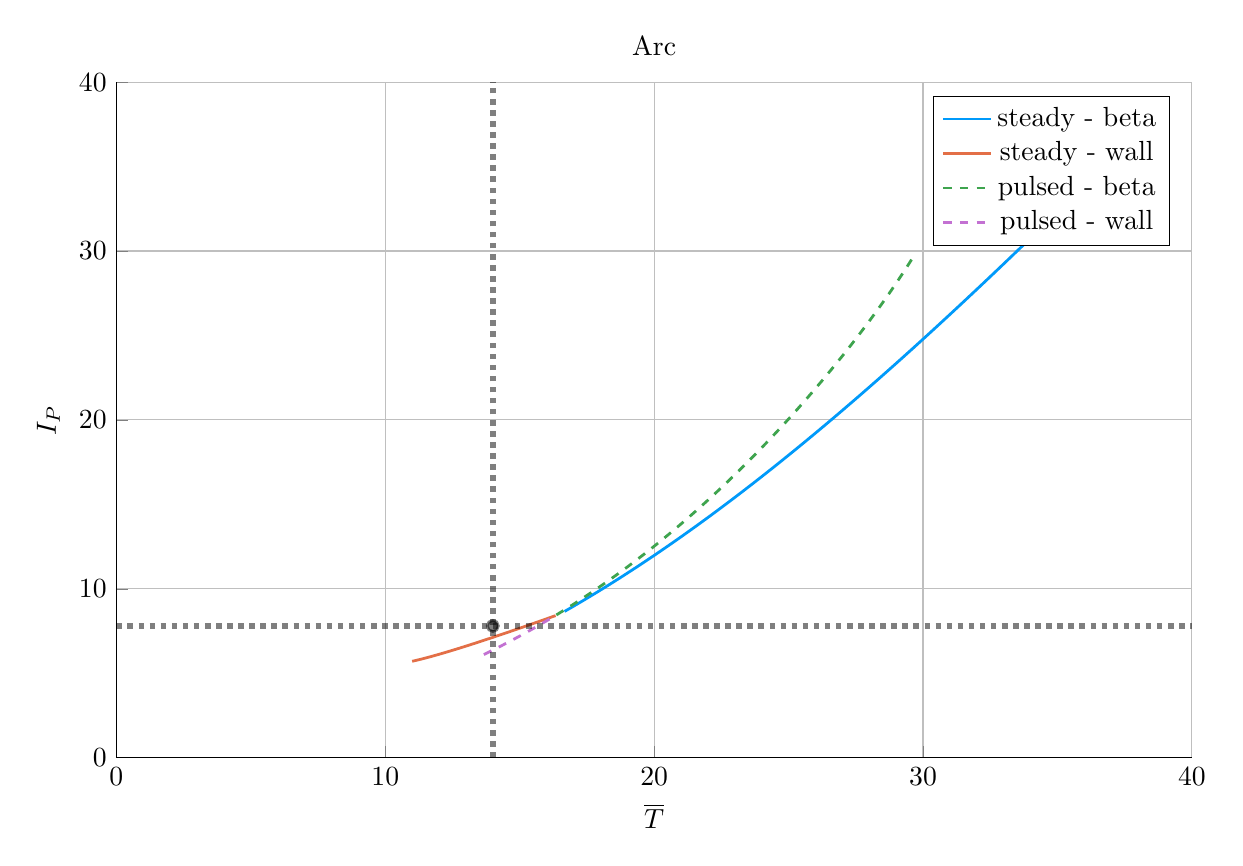
\begin{tikzpicture}[]
\begin{axis}[height = {101.6mm}, ylabel = {$I_P$}, title = {Arc}, xmin = {0.0}, xmax = {40.0}, ymax = {40.0}, xlabel = {$\overline T$}, {unbounded coords=jump, scaled x ticks = false, xticklabel style={rotate = 0}, xmajorgrids = true, xtick = {0.0,10.0,20.0,30.0,40.0}, xticklabels = {0,10,20,30,40}, xtick align = inside, axis lines* = left, scaled y ticks = false, yticklabel style={rotate = 0}, ymajorgrids = true, ytick = {0.0,10.0,20.0,30.0,40.0}, yticklabels = {0,10,20,30,40}, ytick align = inside, axis lines* = left,     xshift = 0.0mm,
    yshift = 0.0mm,
    axis background/.style={fill={rgb,1:red,1.00000000;green,1.00000000;blue,1.00000000}}
}, ymin = {0.0}, width = {152.4mm}]\addplot+ [color = {rgb,1:red,0.00000000;green,0.60560316;blue,0.97868012},
draw opacity=1.0,
line width=1,
solid,mark = none,
mark size = 2.0,
mark options = {
    color = {rgb,1:red,0.00000000;green,0.00000000;blue,0.00000000}, draw opacity = 1.0,
    fill = {rgb,1:red,0.00000000;green,0.60560316;blue,0.97868012}, fill opacity = 1.0,
    line width = 1,
    rotate = 0,
    solid
}]coordinates {
(16.666666666666668, 8.658343870907427)
(17.0, 8.964855141636448)
(17.333333333333332, 9.277118721367206)
(17.666666666666668, 9.595036914426)
(18.0, 9.918585776352757)
(18.333333333333332, 10.247718935951552)
(18.666666666666668, 10.582387319200262)
(19.0, 10.922539274323045)
(19.333333333333332, 11.26812069483817)
(19.666666666666668, 11.61907514056121)
(20.0, 11.975343956529299)
(20.333333333333332, 12.336866389803589)
(20.666666666666668, 12.703579704100664)
(21.0, 13.07541929220057)
(21.333333333333332, 13.452318786079019)
(21.666666666666668, 13.834210164711733)
(22.0, 14.221023859501257)
(22.333333333333332, 14.61268885728139)
(22.666666666666668, 15.009132800857182)
(23.0, 15.410282087044596)
(23.333333333333332, 15.816061962178953)
(23.666666666666668, 16.226396615066992)
(24.0, 16.64120926736311)
(24.333333333333332, 17.060422261356294)
(24.666666666666668, 17.483957145159597)
(25.0, 17.91173475530017)
(25.333333333333332, 18.343675296712746)
(25.666666666666668, 18.77969842014449)
(26.0, 19.2197232969848)
(26.333333333333332, 19.663668691537165)
(26.666666666666668, 20.11145303075519)
(27.0, 20.562994471468567)
(27.333333333333332, 21.018210965128485)
(27.666666666666668, 21.477020320105293)
(28.0, 21.939340261574117)
(28.333333333333332, 22.405088489026962)
(28.666666666666668, 22.874182731452617)
(29.0, 23.34654080022686)
(29.333333333333332, 23.82208063975841)
(29.666666666666668, 24.300720375936947)
(30.0, 24.782378362431352)
(30.333333333333332, 25.26697322488704)
(30.666666666666668, 25.754423903072542)
(31.0, 26.244649691026318)
(31.333333333333332, 26.737570275254438)
(31.666666666666668, 27.233105771031717)
(32.0, 27.731176756857092)
(32.333333333333336, 28.23170430711659)
(32.666666666666664, 28.734610023004112)
(33.0, 29.23981606175298)
(33.333333333333336, 29.747245164229085)
(33.666666666666664, 30.256820680936514)
(34.0, 30.768466596486252)
(34.333333333333336, 31.282107552577845)
(34.666666666666664, 31.797668869543177)
(35.0, 32.31507656650066)
(35.333333333333336, 32.83425738016771)
(35.666666666666664, 33.35513878237846)
(36.0, 33.87764899635294)
(36.333333333333336, 34.40171701176134)
};
\addlegendentry{steady - beta}
\addplot+ [color = {rgb,1:red,0.88887350;green,0.43564919;blue,0.27812294},
draw opacity=1.0,
line width=1,
solid,mark = none,
mark size = 2.0,
mark options = {
    color = {rgb,1:red,0.00000000;green,0.00000000;blue,0.00000000}, draw opacity = 1.0,
    fill = {rgb,1:red,0.88887350;green,0.43564919;blue,0.27812294}, fill opacity = 1.0,
    line width = 1,
    rotate = 0,
    solid
}]coordinates {
(11.0, 5.705363947896813)
(11.333333333333334, 5.831631927327359)
(11.666666666666666, 5.971358416795512)
(12.0, 6.120248050030096)
(12.333333333333334, 6.27635241161913)
(12.666666666666666, 6.438084943966173)
(13.0, 6.6043437111573775)
(13.333333333333334, 6.774432932493379)
(13.666666666666666, 6.9477586358526295)
(14.0, 7.123875039246037)
(14.333333333333334, 7.302428845502918)
(14.666666666666666, 7.483135839919747)
(15.0, 7.66576464137543)
(15.333333333333334, 7.850323804140159)
(15.666666666666666, 8.036059275223955)
(16.0, 8.223435700494395)
(16.333333333333332, 8.412159667095638)
};
\addlegendentry{steady - wall}
\addplot+ [color = {rgb,1:red,0.24222430;green,0.64327509;blue,0.30444865},
draw opacity=1.0,
line width=1,
dashed,mark = none,
mark size = 2.0,
mark options = {
    color = {rgb,1:red,0.00000000;green,0.00000000;blue,0.00000000}, draw opacity = 1.0,
    fill = {rgb,1:red,0.24222430;green,0.64327509;blue,0.30444865}, fill opacity = 1.0,
    line width = 1,
    rotate = 0,
    solid
}]coordinates {
(16.364160609330686, 8.45211123232532)
(16.666666666666668, 8.749174237506722)
(17.0, 9.084875445329175)
(17.333333333333332, 9.429466194729264)
(17.666666666666668, 9.783065958753857)
(18.0, 10.145791398086809)
(18.333333333333332, 10.517756265001724)
(18.666666666666668, 10.899071333792335)
(19.0, 11.28984436597908)
(19.333333333333332, 11.690180120182706)
(19.666666666666668, 12.100180418434789)
(20.0, 12.519944282916168)
(20.333333333333332, 12.949568159742276)
(20.666666666666668, 13.389146249526421)
(21.0, 13.838770968145022)
(21.333333333333332, 14.298533565526986)
(21.666666666666668, 14.768524935556082)
(22.0, 15.2488366565296)
(22.333333333333332, 15.739562309352701)
(22.666666666666668, 16.240799130174846)
(23.0, 16.752650066058415)
(23.333333333333332, 17.27522631730515)
(23.666666666666668, 17.808650469386293)
(24.0, 18.353060342640163)
(24.333333333333332, 18.908613721362002)
(24.666666666666668, 19.475494169025602)
(25.0, 20.053918198206937)
(25.333333333333332, 20.644144149900036)
(25.666666666666668, 21.246483258877372)
(26.0, 21.861313557471373)
(26.333333333333332, 22.48909752802998)
(26.666666666666668, 23.130404800381292)
(27.0, 23.785941781633092)
(27.333333333333332, 24.456591033172632)
(27.666666666666668, 25.143464707502787)
(28.0, 25.84797885666414)
(28.333333333333332, 26.571959755666764)
(28.666666666666668, 27.3178012356156)
(29.0, 28.088707029156687)
(29.333333333333332, 28.889082725820668)
(29.666666666666668, 29.725209471035893)
};
\addlegendentry{pulsed - beta}
\addplot+ [color = {rgb,1:red,0.76444018;green,0.44411178;blue,0.82429754},
draw opacity=1.0,
line width=1,
dashed,mark = none,
mark size = 2.0,
mark options = {
    color = {rgb,1:red,0.00000000;green,0.00000000;blue,0.00000000}, draw opacity = 1.0,
    fill = {rgb,1:red,0.76444018;green,0.44411178;blue,0.82429754}, fill opacity = 1.0,
    line width = 1,
    rotate = 0,
    solid
}]coordinates {
(13.666666666666666, 6.106956435644008)
(14.0, 6.368429153074452)
(14.333333333333334, 6.637611037727747)
(14.666666666666666, 6.914640849606676)
(15.0, 7.199655680909235)
(15.333333333333334, 7.492790823032018)
(15.666666666666666, 7.794179619860046)
(16.0, 8.103953307930404)
(16.333333333333332, 8.422240844292133)
(16.364160609330686, 8.45211123232532)
};
\addlegendentry{pulsed - wall}
\addplot+ [color = {rgb,1:red,0.00000000;green,0.00000000;blue,0.00000000},
draw opacity=0.5,
line width=2,
dotted,mark = none,
mark size = 2.0,
mark options = {
    color = {rgb,1:red,0.00000000;green,0.00000000;blue,0.00000000}, draw opacity = 0.5,
    fill = {rgb,1:red,0.00000000;green,0.00000000;blue,0.00000000}, fill opacity = 0.5,
    line width = 1,
    rotate = 0,
    solid
},forget plot]coordinates {
(0.0, 7.8)
(40.0, 7.8)
};
\addplot+ [color = {rgb,1:red,0.00000000;green,0.00000000;blue,0.00000000},
draw opacity=0.5,
line width=2,
dotted,mark = none,
mark size = 2.0,
mark options = {
    color = {rgb,1:red,0.00000000;green,0.00000000;blue,0.00000000}, draw opacity = 0.5,
    fill = {rgb,1:red,0.00000000;green,0.00000000;blue,0.00000000}, fill opacity = 0.5,
    line width = 1,
    rotate = 0,
    solid
},forget plot]coordinates {
(14.0, 0.0)
(14.0, 40.0)
};
\addplot+[draw=none, color = {rgb,1:red,0.00000000;green,0.00000000;blue,0.00000000},
draw opacity=0.5,
line width=0,
solid,mark = *,
mark size = 2.0,
mark options = {
    color = {rgb,1:red,0.00000000;green,0.00000000;blue,0.00000000}, draw opacity = 0.5,
    fill = {rgb,1:red,0.00000000;green,0.00000000;blue,0.00000000}, fill opacity = 0.5,
    line width = 1,
    rotate = 0,
    solid
},forget plot] coordinates {
(14.0, 7.8)
};
\end{axis}

\end{tikzpicture}

    \end{adjustbox}
        \caption{$I_P$ vs $\overline T$}
    \end{subfigure}
    \hfill \hfill ~\\ ~\\ ~\\
    \caption{Arc Model Comparison} ~\\
\end{figure*}

\begin{table}[h!]
\centering  
\caption{Arc Variables}
\hfill
\begin{subtable}[t]{0.4\textwidth}
\centering  
\caption{Input Variables} ~\\
\begin{tabular}{ c|c } 

Input            & Value           \\
\hline
$H$              & 1.8             \\
$Q$              & 13.6            \\
$N_{G}$          & 0.67            \\
$\epsilon$       & 0.3333          \\
$\kappa_{95}$    & 1.84            \\
$\delta_{95}$    & 0.333           \\
$\nu_{n}$        & 0.385           \\
$\nu_{T}$        & 0.929           \\
$l_{i}$          & 0.67            \\
$A$              & 2.5             \\
$Z_{eff}$        & 1.2             \\
$f_{D}$          & 0.9             \\
$\tau_{FT}$      & 1.6e9           \\
$B_{CS}$         & 12.77           \\

\end{tabular}
\end{subtable}
\hfill
\begin{subtable}[t]{0.5\textwidth}
\centering  
\caption{Output Variables} ~\\
\begin{tabular}{ c|c|c } 

Output           & Original         & Fussy.jl        \\
\hline
$R_{0}$          & 3.3              & 3.382           \\
$B_{0}$          & 9.2              & 9.505           \\
$I_{P}$          & 7.8              & 8.766           \\
$\overline n$    & 1.3              & 1.291           \\
$\overline T$    & 14.0             & 16.78           \\
$\beta_{N}$       & 0.0259           & 0.0259          \\
$q_{95}$         & 7.2              & 6.127           \\
$P_{W}$          & 2.5              & 2.215           \\
$f_{BS}$         & 0.63             & 0.5588          \\
$f_{CD}$         & 0.37             & 0.4412          \\
$f_{IN}$         & -              & -             \\
$\volume$         & 141.0            & 157.4           \\
$P_{F}$          & 525.0            & 725.9           \\
$\eta_{CD}$      & 0.321            & 0.3164          \\

\end{tabular}
\end{subtable}
\hfill
\hfill
\end{table}

\newpage

\subsection{Contrasting with the Aries Act Studies}

\newpage 

\subsubsection{Act I -- Advanced Physics and Engineering}

\begin{figure*}[h!]
    \centering
    \hfill 
    \begin{subfigure}[t]{0.45\textwidth}
        \centering
    \begin{adjustbox}{width=\textwidth}
      \Large
      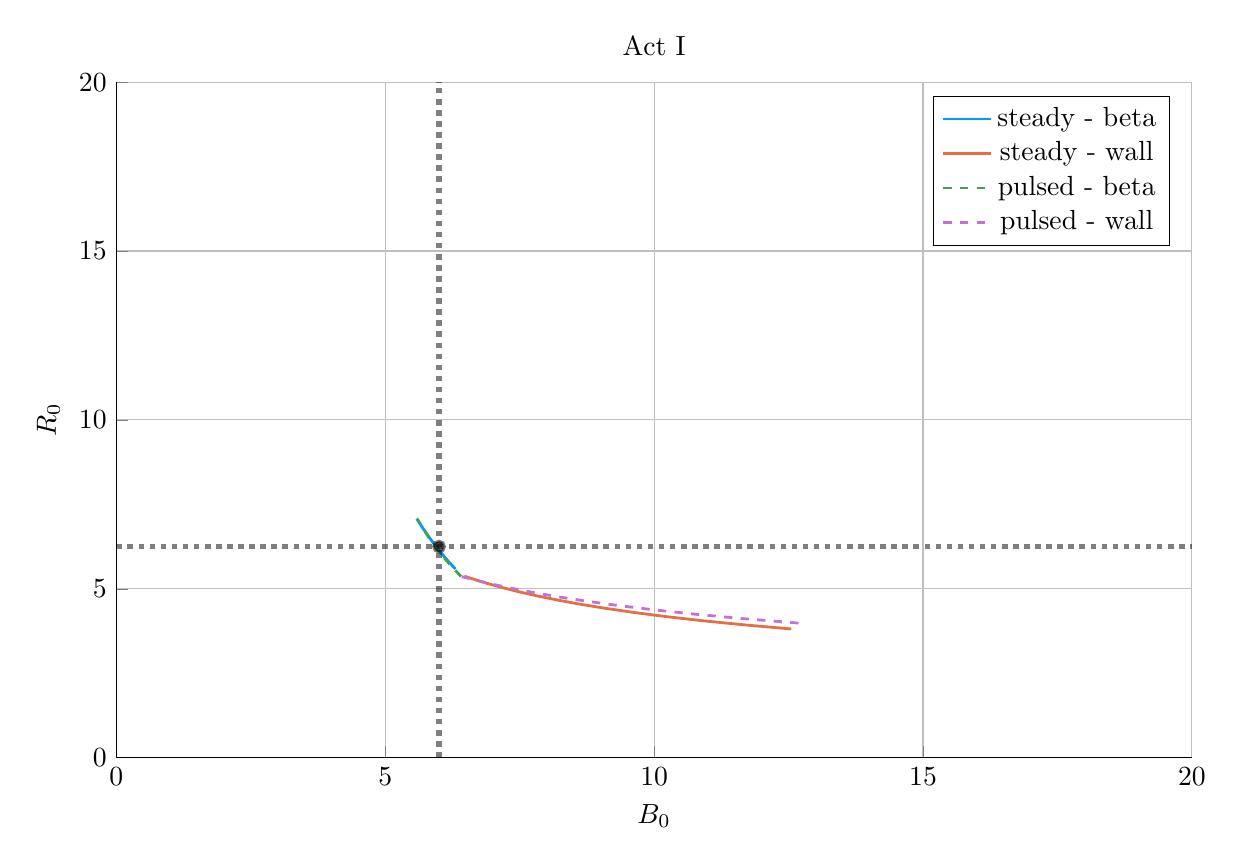
\begin{tikzpicture}[]
\begin{axis}[height = {101.6mm}, ylabel = {$R_0$}, title = {Act I}, xmin = {0.0}, xmax = {20.0}, ymax = {20.0}, xlabel = {$B_0$}, {unbounded coords=jump, scaled x ticks = false, xticklabel style={rotate = 0}, xmajorgrids = true, xtick = {0.0,5.0,10.0,15.0,20.0}, xticklabels = {0,5,10,15,20}, xtick align = inside, axis lines* = left, scaled y ticks = false, yticklabel style={rotate = 0}, ymajorgrids = true, ytick = {0.0,5.0,10.0,15.0,20.0}, yticklabels = {0,5,10,15,20}, ytick align = inside, axis lines* = left,     xshift = 0.0mm,
    yshift = 0.0mm,
    axis background/.style={fill={rgb,1:red,1.00000000;green,1.00000000;blue,1.00000000}}
}, ymin = {0.0}, width = {152.4mm}]\addplot+ [color = {rgb,1:red,0.00000000;green,0.60560316;blue,0.97868012},
draw opacity=1.0,
line width=1,
solid,mark = none,
mark size = 2.0,
mark options = {
    color = {rgb,1:red,0.00000000;green,0.00000000;blue,0.00000000}, draw opacity = 1.0,
    fill = {rgb,1:red,0.00000000;green,0.60560316;blue,0.97868012}, fill opacity = 1.0,
    line width = 1,
    rotate = 0,
    solid
}]coordinates {
(6.30336807958207, 5.587199391496101)
(6.162193069273141, 5.831838137107903)
(6.030717178404645, 6.078157823726375)
(5.908065509576601, 6.325994353145188)
(5.793464904530972, 6.57518910191267)
(5.686229631357383, 6.825588847053452)
(5.585749511271037, 7.077045564754442)
};
\addlegendentry{steady - beta}
\addplot+ [color = {rgb,1:red,0.88887350;green,0.43564919;blue,0.27812294},
draw opacity=1.0,
line width=1,
solid,mark = none,
mark size = 2.0,
mark options = {
    color = {rgb,1:red,0.00000000;green,0.00000000;blue,0.00000000}, draw opacity = 1.0,
    fill = {rgb,1:red,0.88887350;green,0.43564919;blue,0.27812294}, fill opacity = 1.0,
    line width = 1,
    rotate = 0,
    solid
}]coordinates {
(12.549536249695134, 3.8108352245940957)
(11.658754653696462, 3.934083270736017)
(10.883719833507003, 4.057046546594516)
(10.206258129789394, 4.179626810883221)
(9.611335769312953, 4.301750356443285)
(9.086446934250878, 4.423366229113912)
(8.62129895070743, 4.544434218016914)
(8.207216040989662, 4.6649335402400025)
(7.837119555085499, 4.78484200403474)
(7.505047858717157, 4.9041467319817595)
(7.20604322925957, 5.022835870779136)
(6.935884710193303, 5.1409045607718795)
(6.691016583192173, 5.258349129805506)
(6.468415485086983, 5.375167957409874)
};
\addlegendentry{steady - wall}
\addplot+ [color = {rgb,1:red,0.24222430;green,0.64327509;blue,0.30444865},
draw opacity=1.0,
line width=1,
dashed,mark = none,
mark size = 2.0,
mark options = {
    color = {rgb,1:red,0.00000000;green,0.00000000;blue,0.00000000}, draw opacity = 1.0,
    fill = {rgb,1:red,0.24222430;green,0.64327509;blue,0.30444865}, fill opacity = 1.0,
    line width = 1,
    rotate = 0,
    solid
}]coordinates {
(6.408263337806559, 5.366131328829866)
(6.408263337806564, 5.366131328829862)
(6.385466513301022, 5.402805883604879)
(6.245492502072912, 5.638974714472524)
(6.116010320461132, 5.875875066688821)
(5.9960421481916395, 6.113307727774442)
(5.884727159112828, 6.351082733498888)
(5.781304768121868, 6.589019058920955)
(5.685100648450046, 6.826944315253105)
(5.595515000321003, 7.064694456596427)
};
\addlegendentry{pulsed - beta}
\addplot+ [color = {rgb,1:red,0.76444018;green,0.44411178;blue,0.82429754},
draw opacity=1.0,
line width=1,
dashed,mark = none,
mark size = 2.0,
mark options = {
    color = {rgb,1:red,0.00000000;green,0.00000000;blue,0.00000000}, draw opacity = 1.0,
    fill = {rgb,1:red,0.76444018;green,0.44411178;blue,0.82429754}, fill opacity = 1.0,
    line width = 1,
    rotate = 0,
    solid
}]coordinates {
(12.684248532650473, 3.9847907768802657)
(11.66307871570063, 4.114684512780648)
(10.781888309639141, 4.244124103742294)
(10.016282491385791, 4.373086052625054)
(9.346943280276514, 4.501549309887817)
(8.758420158941194, 4.6294950281779785)
(8.238241792953433, 4.756906348757686)
(7.776255600865612, 4.883768212546736)
(7.364131118520045, 5.010067192354689)
(6.994982564641668, 5.135791343697217)
(6.66307916140573, 5.260930071474144)
(6.408263337806559, 5.366131328829866)
(6.408263337806564, 5.366131328829862)
};
\addlegendentry{pulsed - wall}
\addplot+ [color = {rgb,1:red,0.00000000;green,0.00000000;blue,0.00000000},
draw opacity=0.5,
line width=2,
dotted,mark = none,
mark size = 2.0,
mark options = {
    color = {rgb,1:red,0.00000000;green,0.00000000;blue,0.00000000}, draw opacity = 0.5,
    fill = {rgb,1:red,0.00000000;green,0.00000000;blue,0.00000000}, fill opacity = 0.5,
    line width = 1,
    rotate = 0,
    solid
},forget plot]coordinates {
(0.0, 6.25)
(20.0, 6.25)
};
\addplot+ [color = {rgb,1:red,0.00000000;green,0.00000000;blue,0.00000000},
draw opacity=0.5,
line width=2,
dotted,mark = none,
mark size = 2.0,
mark options = {
    color = {rgb,1:red,0.00000000;green,0.00000000;blue,0.00000000}, draw opacity = 0.5,
    fill = {rgb,1:red,0.00000000;green,0.00000000;blue,0.00000000}, fill opacity = 0.5,
    line width = 1,
    rotate = 0,
    solid
},forget plot]coordinates {
(6.0, 0.0)
(6.0, 20.0)
};
\addplot+[draw=none, color = {rgb,1:red,0.00000000;green,0.00000000;blue,0.00000000},
draw opacity=0.5,
line width=0,
solid,mark = *,
mark size = 2.0,
mark options = {
    color = {rgb,1:red,0.00000000;green,0.00000000;blue,0.00000000}, draw opacity = 0.5,
    fill = {rgb,1:red,0.00000000;green,0.00000000;blue,0.00000000}, fill opacity = 0.5,
    line width = 1,
    rotate = 0,
    solid
},forget plot] coordinates {
(6.0, 6.25)
};
\end{axis}

\end{tikzpicture}

    \end{adjustbox}
        \caption{$R_0$ vs $B_0$}
    \end{subfigure}
    \hfill
    \begin{subfigure}[t]{0.45\textwidth}
        \centering
    \begin{adjustbox}{width=\textwidth}
      \Large
      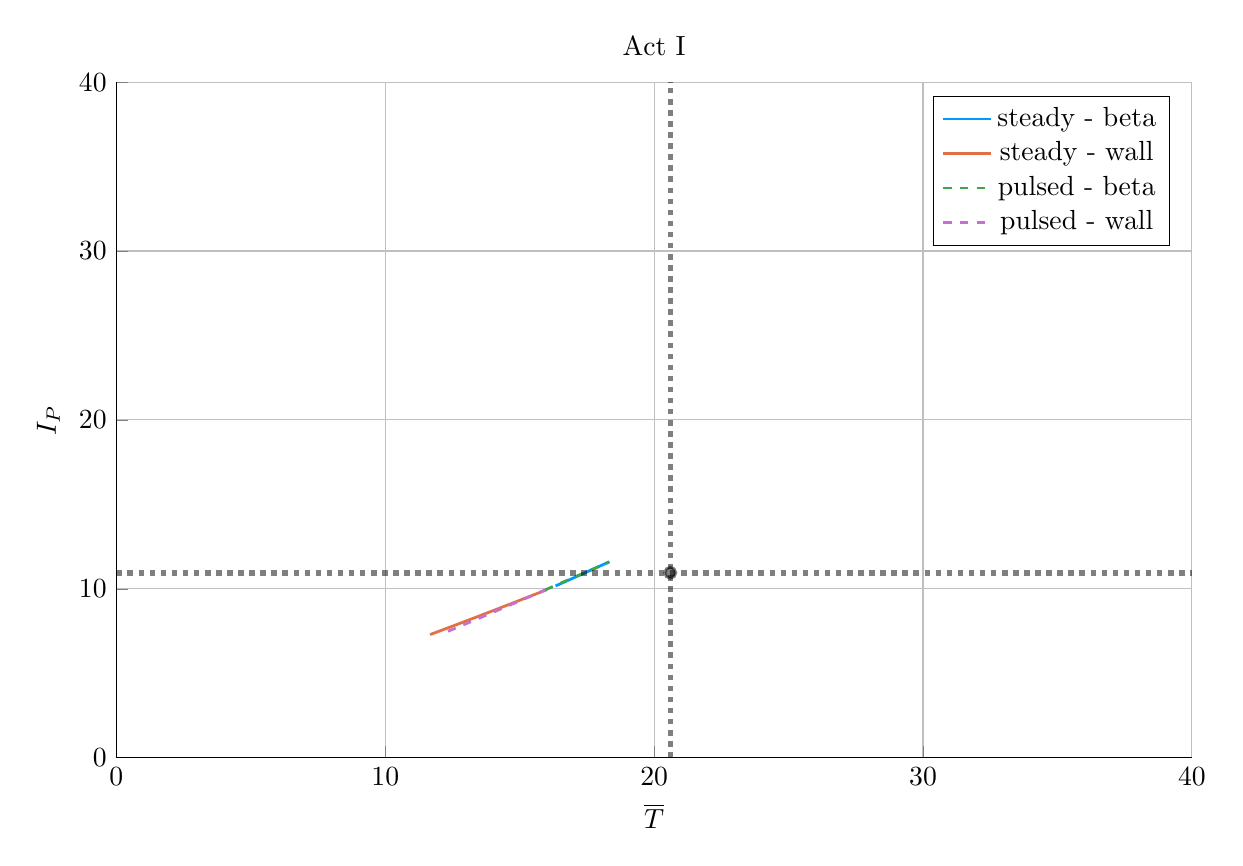
\begin{tikzpicture}[]
\begin{axis}[height = {101.6mm}, ylabel = {$I_P$}, title = {Act I}, xmin = {0.0}, xmax = {40.0}, ymax = {40.0}, xlabel = {$\overline T$}, {unbounded coords=jump, scaled x ticks = false, xticklabel style={rotate = 0}, xmajorgrids = true, xtick = {0.0,10.0,20.0,30.0,40.0}, xticklabels = {0,10,20,30,40}, xtick align = inside, axis lines* = left, scaled y ticks = false, yticklabel style={rotate = 0}, ymajorgrids = true, ytick = {0.0,10.0,20.0,30.0,40.0}, yticklabels = {0,10,20,30,40}, ytick align = inside, axis lines* = left,     xshift = 0.0mm,
    yshift = 0.0mm,
    axis background/.style={fill={rgb,1:red,1.00000000;green,1.00000000;blue,1.00000000}}
}, ymin = {0.0}, width = {152.4mm}]\addplot+ [color = {rgb,1:red,0.00000000;green,0.60560316;blue,0.97868012},
draw opacity=1.0,
line width=1,
solid,mark = none,
mark size = 2.0,
mark options = {
    color = {rgb,1:red,0.00000000;green,0.00000000;blue,0.00000000}, draw opacity = 1.0,
    fill = {rgb,1:red,0.00000000;green,0.60560316;blue,0.97868012}, fill opacity = 1.0,
    line width = 1,
    rotate = 0,
    solid
}]coordinates {
(16.333333333333332, 10.169194435531358)
(16.666666666666668, 10.405057509328124)
(17.0, 10.641905327194731)
(17.333333333333332, 10.87971637136811)
(17.666666666666668, 11.11846917050157)
(18.0, 11.358142407296011)
(18.333333333333332, 11.598714938197329)
};
\addlegendentry{steady - beta}
\addplot+ [color = {rgb,1:red,0.88887350;green,0.43564919;blue,0.27812294},
draw opacity=1.0,
line width=1,
solid,mark = none,
mark size = 2.0,
mark options = {
    color = {rgb,1:red,0.00000000;green,0.00000000;blue,0.00000000}, draw opacity = 1.0,
    fill = {rgb,1:red,0.88887350;green,0.43564919;blue,0.27812294}, fill opacity = 1.0,
    line width = 1,
    rotate = 0,
    solid
}]coordinates {
(11.666666666666666, 7.287903136887)
(12.0, 7.486025430610099)
(12.333333333333334, 7.685696663157812)
(12.666666666666666, 7.886645361110723)
(13.0, 8.08866940687473)
(13.333333333333334, 8.291629426976055)
(13.666666666666666, 8.495414075666067)
(14.0, 8.699964056113311)
(14.333333333333334, 8.905213556979005)
(14.666666666666666, 9.111120468746519)
(15.0, 9.31764336053339)
(15.333333333333334, 9.524758318501357)
(15.666666666666666, 9.732442959434447)
(16.0, 9.940679052729761)
};
\addlegendentry{steady - wall}
\addplot+ [color = {rgb,1:red,0.24222430;green,0.64327509;blue,0.30444865},
draw opacity=1.0,
line width=1,
dashed,mark = none,
mark size = 2.0,
mark options = {
    color = {rgb,1:red,0.00000000;green,0.00000000;blue,0.00000000}, draw opacity = 1.0,
    fill = {rgb,1:red,0.24222430;green,0.64327509;blue,0.30444865}, fill opacity = 1.0,
    line width = 1,
    rotate = 0,
    solid
}]coordinates {
(15.948125117373092, 9.933500150990564)
(15.9481251173731, 9.933500150990564)
(16.0, 9.969282740147014)
(16.333333333333332, 10.199548426407084)
(16.666666666666668, 10.430379144484162)
(17.0, 10.661750348679098)
(17.333333333333332, 10.893638132753678)
(17.666666666666668, 11.126019229767902)
(18.0, 11.358871009413285)
(18.333333333333332, 11.592171473618816)
};
\addlegendentry{pulsed - beta}
\addplot+ [color = {rgb,1:red,0.76444018;green,0.44411178;blue,0.82429754},
draw opacity=1.0,
line width=1,
dashed,mark = none,
mark size = 2.0,
mark options = {
    color = {rgb,1:red,0.00000000;green,0.00000000;blue,0.00000000}, draw opacity = 1.0,
    fill = {rgb,1:red,0.76444018;green,0.44411178;blue,0.82429754}, fill opacity = 1.0,
    line width = 1,
    rotate = 0,
    solid
}]coordinates {
(12.333333333333334, 7.481290856821823)
(12.666666666666666, 7.703549290655078)
(13.0, 7.92668121689452)
(13.333333333333334, 8.15065615613957)
(13.666666666666666, 8.375443966327172)
(14.0, 8.601014900773066)
(14.333333333333334, 8.82733966430566)
(14.666666666666666, 9.054389459546684)
(15.0, 9.282136024328327)
(15.333333333333334, 9.510551661584085)
(15.666666666666666, 9.73960926266661)
(15.948125117373092, 9.933500150990564)
(15.9481251173731, 9.933500150990564)
};
\addlegendentry{pulsed - wall}
\addplot+ [color = {rgb,1:red,0.00000000;green,0.00000000;blue,0.00000000},
draw opacity=0.5,
line width=2,
dotted,mark = none,
mark size = 2.0,
mark options = {
    color = {rgb,1:red,0.00000000;green,0.00000000;blue,0.00000000}, draw opacity = 0.5,
    fill = {rgb,1:red,0.00000000;green,0.00000000;blue,0.00000000}, fill opacity = 0.5,
    line width = 1,
    rotate = 0,
    solid
},forget plot]coordinates {
(0.0, 10.95)
(40.0, 10.95)
};
\addplot+ [color = {rgb,1:red,0.00000000;green,0.00000000;blue,0.00000000},
draw opacity=0.5,
line width=2,
dotted,mark = none,
mark size = 2.0,
mark options = {
    color = {rgb,1:red,0.00000000;green,0.00000000;blue,0.00000000}, draw opacity = 0.5,
    fill = {rgb,1:red,0.00000000;green,0.00000000;blue,0.00000000}, fill opacity = 0.5,
    line width = 1,
    rotate = 0,
    solid
},forget plot]coordinates {
(20.6, 0.0)
(20.6, 40.0)
};
\addplot+[draw=none, color = {rgb,1:red,0.00000000;green,0.00000000;blue,0.00000000},
draw opacity=0.5,
line width=0,
solid,mark = *,
mark size = 2.0,
mark options = {
    color = {rgb,1:red,0.00000000;green,0.00000000;blue,0.00000000}, draw opacity = 0.5,
    fill = {rgb,1:red,0.00000000;green,0.00000000;blue,0.00000000}, fill opacity = 0.5,
    line width = 1,
    rotate = 0,
    solid
},forget plot] coordinates {
(20.6, 10.95)
};
\end{axis}

\end{tikzpicture}

    \end{adjustbox}
        \caption{$I_P$ vs $\overline T$}
    \end{subfigure}
    \hfill \hfill ~\\ ~\\ ~\\
    \caption{Aries Act I Model Comparison} ~\\
\end{figure*}

\begin{table}[h!]
\centering  
\caption{Act I Variables}
\hfill
\begin{subtable}[t]{0.4\textwidth}
\centering  
\caption{Input Variables} ~\\
\begin{tabular}{ c|c } 

Input            & Value           \\
\hline
$H$              & 1.65            \\
$Q$              & 42.5            \\
$N_{G}$          & 1.0             \\
$\epsilon$       & 0.25            \\
$\kappa_{95}$    & 2.1             \\
$\delta_{95}$    & 0.4             \\
$\nu_{n}$        & 0.27            \\
$\nu_{T}$        & 1.15            \\
$l_{i}$          & 0.35906         \\
$A$              & 2.5             \\
$Z_{eff}$        & 2.11            \\
$f_{D}$          & 0.75            \\
$\tau_{FT}$      & 1.6e9           \\
$B_{CS}$         & 12.77           \\

\end{tabular}
\end{subtable}
\hfill
\begin{subtable}[t]{0.5\textwidth}
\centering  
\caption{Output Variables} ~\\
\begin{tabular}{ c|c|c } 

Output           & Original         & Fussy.jl        \\
\hline
$R_{0}$          & 6.25             & 6.226           \\
$B_{0}$          & 6.0              & 5.956           \\
$I_{P}$          & 10.95            & 10.78           \\
$\overline n$    & 1.3              & 1.288           \\
$\overline T$    & 20.6             & 17.2            \\
$\beta_{N}$       & 0.0427           & 0.0427          \\
$q_{95}$         & 4.5              & 3.993           \\
$P_{W}$          & 2.45             & 2.004           \\
$f_{BS}$         & 0.91             & 0.906           \\
$f_{CD}$         & 0.09             & 0.094           \\
$f_{IN}$         & -              & -             \\
$\volume$         & 582.0            & 621.4           \\
$P_{F}$          & 1813           & 1865          \\
$\eta_{CD}$      & 0.188            & 0.1853          \\

\end{tabular}
\end{subtable}
\hfill
\hfill
\end{table}

\newpage 

\subsubsection{Act II -- Conservative Physics and Engineering}

\begin{figure*}[h!]
    \centering
    \hfill 
    \begin{subfigure}[t]{0.45\textwidth}
        \centering
    \begin{adjustbox}{width=\textwidth}
      \Large
      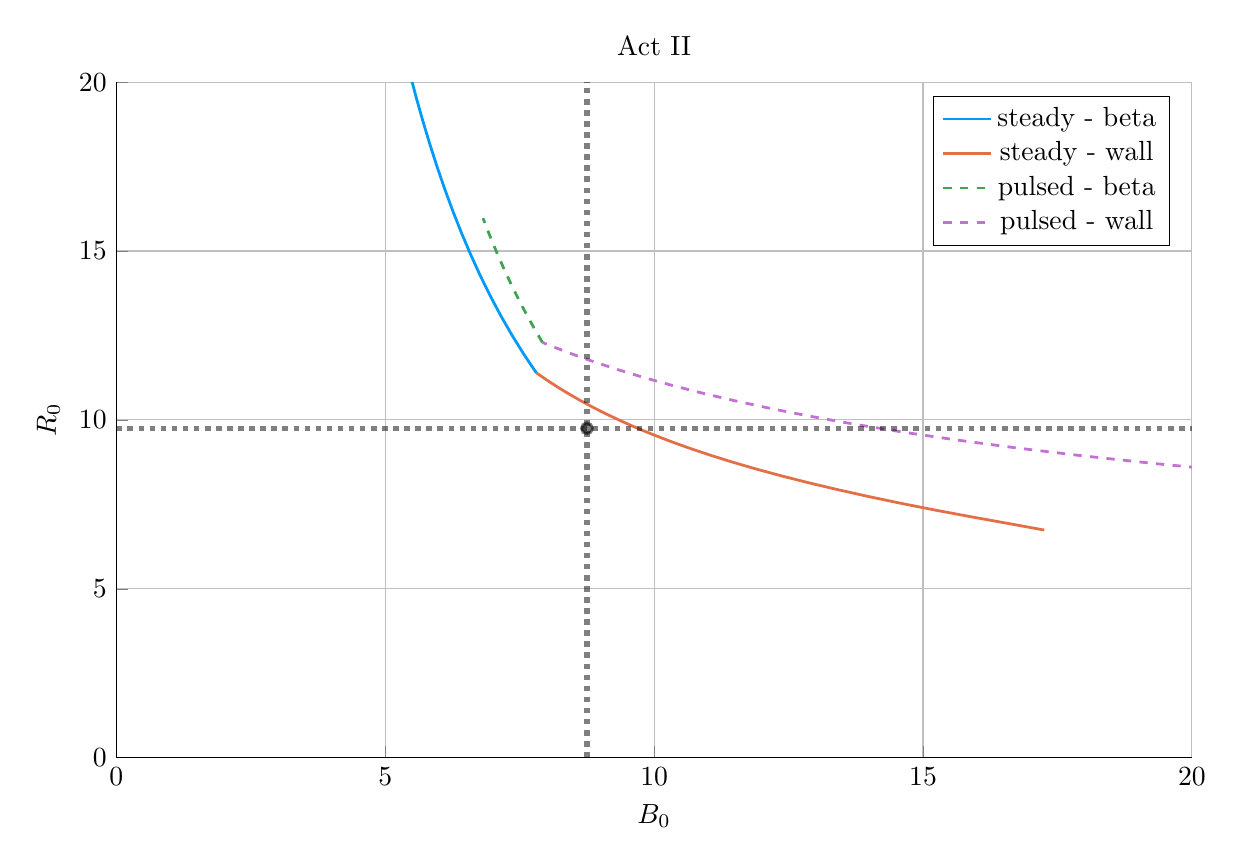
\begin{tikzpicture}[]
\begin{axis}[height = {101.6mm}, ylabel = {$R_0$}, title = {Act II}, xmin = {0.0}, xmax = {20.0}, ymax = {20.0}, xlabel = {$B_0$}, {unbounded coords=jump, scaled x ticks = false, xticklabel style={rotate = 0}, xmajorgrids = true, xtick = {0.0,5.0,10.0,15.0,20.0}, xticklabels = {0,5,10,15,20}, xtick align = inside, axis lines* = left, scaled y ticks = false, yticklabel style={rotate = 0}, ymajorgrids = true, ytick = {0.0,5.0,10.0,15.0,20.0}, yticklabels = {0,5,10,15,20}, ytick align = inside, axis lines* = left,     xshift = 0.0mm,
    yshift = 0.0mm,
    axis background/.style={fill={rgb,1:red,1.00000000;green,1.00000000;blue,1.00000000}}
}, ymin = {0.0}, width = {152.4mm}]\addplot+ [color = {rgb,1:red,0.00000000;green,0.60560316;blue,0.97868012},
draw opacity=1.0,
line width=1,
solid,mark = none,
mark size = 2.0,
mark options = {
    color = {rgb,1:red,0.00000000;green,0.00000000;blue,0.00000000}, draw opacity = 1.0,
    fill = {rgb,1:red,0.00000000;green,0.60560316;blue,0.97868012}, fill opacity = 1.0,
    line width = 1,
    rotate = 0,
    solid
}]coordinates {
(7.810935944285959, 11.389141268081966)
(7.57736049850867, 11.942634046586162)
(7.354864292609041, 12.51245847357923)
(7.145167234136329, 13.0943365692581)
(6.9473303865083675, 13.687993788149779)
(6.760499508614096, 14.293145886478186)
(6.583897990324067, 14.909495325365516)
(6.416817229618043, 15.536734694045393)
(6.258609820663305, 16.1745467994937)
(6.108683264880386, 16.82260538899235)
(5.966494431410919, 17.480575868750975)
(5.831544666176381, 18.148116014600475)
(5.703375459679132, 18.824876684423757)
(5.581564609582325, 19.510502502077443)
(5.465722802994068, 20.20463254880097)
(5.355490573482678, 20.906901035327614)
(5.25053558682053, 21.616937949657327)
(5.1505502068221745, 22.334369714080776)
(5.0552493196883175, 23.058819802110854)
};
\addlegendentry{steady - beta}
\addplot+ [color = {rgb,1:red,0.88887350;green,0.43564919;blue,0.27812294},
draw opacity=1.0,
line width=1,
solid,mark = none,
mark size = 2.0,
mark options = {
    color = {rgb,1:red,0.00000000;green,0.00000000;blue,0.00000000}, draw opacity = 1.0,
    fill = {rgb,1:red,0.88887350;green,0.43564919;blue,0.27812294}, fill opacity = 1.0,
    line width = 1,
    rotate = 0,
    solid
}]coordinates {
(17.25550839059296, 6.738604635617289)
(16.594334962335296, 6.931178286222189)
(15.9071755430688, 7.128187388035985)
(15.233983138507648, 7.327817939330552)
(14.594239858921854, 7.528927553154291)
(13.989673082630297, 7.7312042898700515)
(13.414782495717416, 7.934790159202381)
(12.872659546281994, 8.139273115071695)
(12.364365715508608, 8.344321605506495)
(11.889507953196574, 8.549679244077495)
(11.44685939646348, 8.755144058838903)
(11.034739998180656, 8.960554762148757)
(10.651252523287319, 9.165781242855727)
(10.294428800132035, 9.370717743724994)
(9.962319203963213, 9.57527782549947)
(9.653045819449929, 9.779390564591205)
(9.364832254395445, 9.982997628553138)
(9.096018465506306, 10.186050992034668)
(8.844373144802077, 10.388606525997883)
(8.61055754360846, 10.590345571972314)
(8.391192178573277, 10.791527736428888)
(8.18577947665566, 10.992035979756642)
(7.99323348423048, 11.1918525509058)
(7.812301489248497, 11.391007917726574)
};
\addlegendentry{steady - wall}
\addplot+ [color = {rgb,1:red,0.24222430;green,0.64327509;blue,0.30444865},
draw opacity=1.0,
line width=1,
dashed,mark = none,
mark size = 2.0,
mark options = {
    color = {rgb,1:red,0.00000000;green,0.00000000;blue,0.00000000}, draw opacity = 1.0,
    fill = {rgb,1:red,0.24222430;green,0.64327509;blue,0.30444865}, fill opacity = 1.0,
    line width = 1,
    rotate = 0,
    solid
}]coordinates {
(7.923668284887995, 12.293879059492616)
(7.923668284887995, 12.293879059492635)
(7.836759696043437, 12.52591633746021)
(7.6662731560983355, 13.00454403942661)
(7.50499428233835, 13.488375025456907)
(7.35232773269976, 13.977065733125242)
(7.207727224738343, 14.470269937628656)
(7.070690693175276, 14.967639476613451)
(6.940756001029682, 15.46882496625731)
(6.817497143644154, 15.973476480630131)
};
\addlegendentry{pulsed - beta}
\addplot+ [color = {rgb,1:red,0.76444018;green,0.44411178;blue,0.82429754},
draw opacity=1.0,
line width=1,
dashed,mark = none,
mark size = 2.0,
mark options = {
    color = {rgb,1:red,0.00000000;green,0.00000000;blue,0.00000000}, draw opacity = 1.0,
    fill = {rgb,1:red,0.76444018;green,0.44411178;blue,0.82429754}, fill opacity = 1.0,
    line width = 1,
    rotate = 0,
    solid
}]coordinates {
(22.56106430311702, 8.239911323116141)
(20.85607192394036, 8.471453471694678)
(19.335265246056654, 8.703260993170346)
(17.974121547130903, 8.935277031603567)
(16.751976718553127, 9.167446093344447)
(15.651329744019142, 9.399714010238458)
(14.65728744097675, 9.632027927077594)
(13.757118584462601, 9.864336290607328)
(12.939893642194303, 10.096588839007167)
(12.196191964860315, 10.328736591776112)
(11.517862472405039, 10.560731839999896)
(10.897827027335556, 10.792528137074703)
(10.329918077124672, 11.02408028901105)
(9.808743940706389, 11.255344346143936)
(9.329576544487265, 11.486277593626015)
(8.888257451278507, 11.716838542453242)
(8.481118883411932, 11.946986920205564)
(8.10491708701527, 12.17668366154026)
(7.923668284887995, 12.293879059492616)
(7.923668284887995, 12.293879059492635)
};
\addlegendentry{pulsed - wall}
\addplot+ [color = {rgb,1:red,0.00000000;green,0.00000000;blue,0.00000000},
draw opacity=0.5,
line width=2,
dotted,mark = none,
mark size = 2.0,
mark options = {
    color = {rgb,1:red,0.00000000;green,0.00000000;blue,0.00000000}, draw opacity = 0.5,
    fill = {rgb,1:red,0.00000000;green,0.00000000;blue,0.00000000}, fill opacity = 0.5,
    line width = 1,
    rotate = 0,
    solid
},forget plot]coordinates {
(0.0, 9.75)
(20.0, 9.75)
};
\addplot+ [color = {rgb,1:red,0.00000000;green,0.00000000;blue,0.00000000},
draw opacity=0.5,
line width=2,
dotted,mark = none,
mark size = 2.0,
mark options = {
    color = {rgb,1:red,0.00000000;green,0.00000000;blue,0.00000000}, draw opacity = 0.5,
    fill = {rgb,1:red,0.00000000;green,0.00000000;blue,0.00000000}, fill opacity = 0.5,
    line width = 1,
    rotate = 0,
    solid
},forget plot]coordinates {
(8.75, 0.0)
(8.75, 20.0)
};
\addplot+[draw=none, color = {rgb,1:red,0.00000000;green,0.00000000;blue,0.00000000},
draw opacity=0.5,
line width=0,
solid,mark = *,
mark size = 2.0,
mark options = {
    color = {rgb,1:red,0.00000000;green,0.00000000;blue,0.00000000}, draw opacity = 0.5,
    fill = {rgb,1:red,0.00000000;green,0.00000000;blue,0.00000000}, fill opacity = 0.5,
    line width = 1,
    rotate = 0,
    solid
},forget plot] coordinates {
(8.75, 9.75)
};
\end{axis}

\end{tikzpicture}

    \end{adjustbox}
        \caption{$R_0$ vs $B_0$}
    \end{subfigure}
    \hfill
    \begin{subfigure}[t]{0.45\textwidth}
        \centering
    \begin{adjustbox}{width=\textwidth}
      \Large
      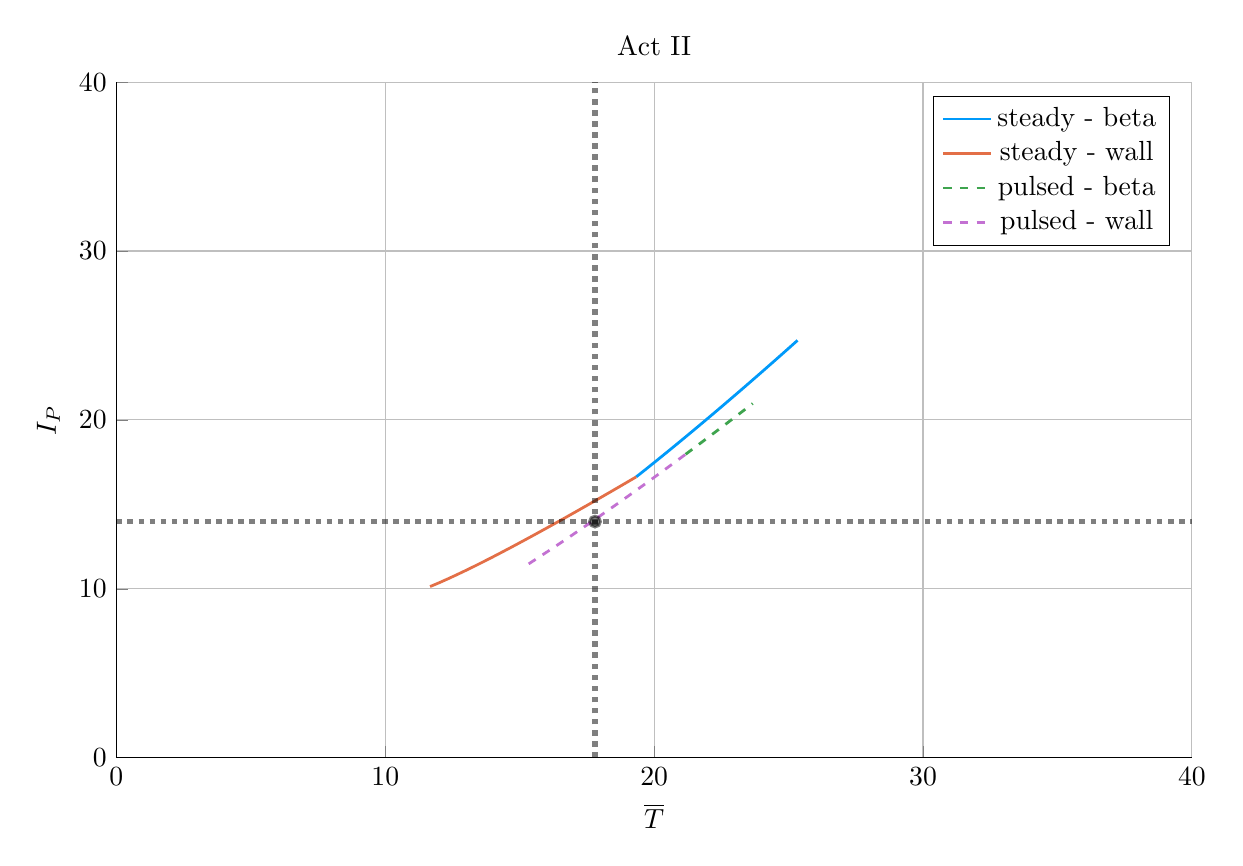
\begin{tikzpicture}[]
\begin{axis}[height = {101.6mm}, ylabel = {$I_P$}, title = {Act II}, xmin = {0.0}, xmax = {40.0}, ymax = {40.0}, xlabel = {$\overline T$}, {unbounded coords=jump, scaled x ticks = false, xticklabel style={rotate = 0}, xmajorgrids = true, xtick = {0.0,10.0,20.0,30.0,40.0}, xticklabels = {0,10,20,30,40}, xtick align = inside, axis lines* = left, scaled y ticks = false, yticklabel style={rotate = 0}, ymajorgrids = true, ytick = {0.0,10.0,20.0,30.0,40.0}, yticklabels = {0,10,20,30,40}, ytick align = inside, axis lines* = left,     xshift = 0.0mm,
    yshift = 0.0mm,
    axis background/.style={fill={rgb,1:red,1.00000000;green,1.00000000;blue,1.00000000}}
}, ymin = {0.0}, width = {152.4mm}]\addplot+ [color = {rgb,1:red,0.00000000;green,0.60560316;blue,0.97868012},
draw opacity=1.0,
line width=1,
solid,mark = none,
mark size = 2.0,
mark options = {
    color = {rgb,1:red,0.00000000;green,0.00000000;blue,0.00000000}, draw opacity = 1.0,
    fill = {rgb,1:red,0.00000000;green,0.60560316;blue,0.97868012}, fill opacity = 1.0,
    line width = 1,
    rotate = 0,
    solid
}]coordinates {
(19.333333333333332, 16.626976584120992)
(19.666666666666668, 17.04714126565062)
(20.0, 17.4728205159228)
(20.333333333333332, 17.902037802268676)
(20.666666666666668, 18.334710756318135)
(21.0, 18.770758343299946)
(21.333333333333332, 19.21009903030823)
(21.666666666666668, 19.652652028291016)
(22.0, 20.098337062332053)
(22.333333333333332, 20.547074418426956)
(22.666666666666668, 20.998784986741654)
(23.0, 21.453390301179443)
(23.333333333333332, 21.910812577709113)
(23.666666666666668, 22.37097474604109)
(24.0, 22.833800482195542)
(24.333333333333332, 23.299214237115898)
(24.666666666666668, 23.767141260842724)
(25.0, 24.237507628970306)
(25.333333333333332, 24.710240262329886)
};
\addlegendentry{steady - beta}
\addplot+ [color = {rgb,1:red,0.88887350;green,0.43564919;blue,0.27812294},
draw opacity=1.0,
line width=1,
solid,mark = none,
mark size = 2.0,
mark options = {
    color = {rgb,1:red,0.00000000;green,0.00000000;blue,0.00000000}, draw opacity = 1.0,
    fill = {rgb,1:red,0.88887350;green,0.43564919;blue,0.27812294}, fill opacity = 1.0,
    line width = 1,
    rotate = 0,
    solid
}]coordinates {
(11.666666666666666, 10.131702672149428)
(12.0, 10.354462623384137)
(12.333333333333334, 10.591104956642406)
(12.666666666666666, 10.837356598740662)
(13.0, 11.09054386610192)
(13.333333333333334, 11.349883742416331)
(13.666666666666666, 11.61561327802365)
(14.0, 11.886764241828663)
(14.333333333333334, 12.16256217004895)
(14.666666666666666, 12.44240841774136)
(15.0, 12.72583049098312)
(15.333333333333334, 13.012449288635679)
(15.666666666666666, 13.301956539143166)
(16.0, 13.59409872387861)
(16.333333333333332, 13.888665310111481)
(16.666666666666668, 14.185479949266789)
(17.0, 14.48439377498311)
(17.333333333333332, 14.785280223642218)
(17.666666666666668, 15.088238807947413)
(18.0, 15.392552774473998)
(18.333333333333332, 15.698764813772398)
(18.666666666666668, 16.00659672680533)
(19.0, 16.315986303185774)
(19.333333333333332, 16.626976584120992)
};
\addlegendentry{steady - wall}
\addplot+ [color = {rgb,1:red,0.24222430;green,0.64327509;blue,0.30444865},
draw opacity=1.0,
line width=1,
dashed,mark = none,
mark size = 2.0,
mark options = {
    color = {rgb,1:red,0.00000000;green,0.00000000;blue,0.00000000}, draw opacity = 1.0,
    fill = {rgb,1:red,0.24222430;green,0.64327509;blue,0.30444865}, fill opacity = 1.0,
    line width = 1,
    rotate = 0,
    solid
}]coordinates {
(21.17034352159018, 17.96627417153032)
(21.170343521590212, 17.966274171530337)
(21.333333333333332, 18.1591936305205)
(21.666666666666668, 18.555297107283753)
(22.0, 18.953426399022014)
(22.333333333333332, 19.353497539767794)
(22.666666666666668, 19.7554274455778)
(23.0, 20.159133974954596)
(23.333333333333332, 20.564535986760628)
(23.666666666666668, 20.971553389451927)
};
\addlegendentry{pulsed - beta}
\addplot+ [color = {rgb,1:red,0.76444018;green,0.44411178;blue,0.82429754},
draw opacity=1.0,
line width=1,
dashed,mark = none,
mark size = 2.0,
mark options = {
    color = {rgb,1:red,0.00000000;green,0.00000000;blue,0.00000000}, draw opacity = 1.0,
    fill = {rgb,1:red,0.76444018;green,0.44411178;blue,0.82429754}, fill opacity = 1.0,
    line width = 1,
    rotate = 0,
    solid
}]coordinates {
(15.333333333333334, 11.474678053719876)
(15.666666666666666, 11.819475032994422)
(16.0, 12.167858357397087)
(16.333333333333332, 12.51974460671026)
(16.666666666666668, 12.875049128346197)
(17.0, 13.233686175102404)
(17.333333333333332, 13.595569077154208)
(17.666666666666668, 13.96061040317257)
(18.0, 14.328722110173729)
(18.333333333333332, 14.699815683529526)
(18.666666666666668, 15.073802268415148)
(19.0, 15.450592793824576)
(19.333333333333332, 15.830098089115069)
(19.666666666666668, 16.21222899561205)
(20.0, 16.596896471191773)
(20.333333333333332, 16.984011690059134)
(20.666666666666668, 17.37348613728185)
(21.0, 17.765231698435688)
(21.17034352159018, 17.96627417153032)
(21.170343521590212, 17.966274171530337)
};
\addlegendentry{pulsed - wall}
\addplot+ [color = {rgb,1:red,0.00000000;green,0.00000000;blue,0.00000000},
draw opacity=0.5,
line width=2,
dotted,mark = none,
mark size = 2.0,
mark options = {
    color = {rgb,1:red,0.00000000;green,0.00000000;blue,0.00000000}, draw opacity = 0.5,
    fill = {rgb,1:red,0.00000000;green,0.00000000;blue,0.00000000}, fill opacity = 0.5,
    line width = 1,
    rotate = 0,
    solid
},forget plot]coordinates {
(0.0, 13.98)
(40.0, 13.98)
};
\addplot+ [color = {rgb,1:red,0.00000000;green,0.00000000;blue,0.00000000},
draw opacity=0.5,
line width=2,
dotted,mark = none,
mark size = 2.0,
mark options = {
    color = {rgb,1:red,0.00000000;green,0.00000000;blue,0.00000000}, draw opacity = 0.5,
    fill = {rgb,1:red,0.00000000;green,0.00000000;blue,0.00000000}, fill opacity = 0.5,
    line width = 1,
    rotate = 0,
    solid
},forget plot]coordinates {
(17.8, 0.0)
(17.8, 40.0)
};
\addplot+[draw=none, color = {rgb,1:red,0.00000000;green,0.00000000;blue,0.00000000},
draw opacity=0.5,
line width=0,
solid,mark = *,
mark size = 2.0,
mark options = {
    color = {rgb,1:red,0.00000000;green,0.00000000;blue,0.00000000}, draw opacity = 0.5,
    fill = {rgb,1:red,0.00000000;green,0.00000000;blue,0.00000000}, fill opacity = 0.5,
    line width = 1,
    rotate = 0,
    solid
},forget plot] coordinates {
(17.8, 13.98)
};
\end{axis}

\end{tikzpicture}

    \end{adjustbox}
        \caption{$I_P$ vs $\overline T$}
    \end{subfigure}
    \hfill \hfill ~\\ ~\\ ~\\
    \caption{Aries Act II Model Comparison} ~\\
\end{figure*}

\begin{table}[h!]
\centering  
\caption{Act II Variables}
\hfill
\begin{subtable}[t]{0.4\textwidth}
\centering  
\caption{Input Variables} ~\\
\begin{tabular}{ c|c } 

Input            & Value           \\
\hline
$H$              & 1.22            \\
$Q$              & 25.0            \\
$N_{G}$          & 1.3             \\
$\epsilon$       & 0.25            \\
$\kappa_{95}$    & 1.964           \\
$\delta_{95}$    & 0.42            \\
$\nu_{n}$        & 0.41            \\
$\nu_{T}$        & 1.15            \\
$l_{i}$          & 0.60275         \\
$A$              & 2.5             \\
$Z_{eff}$        & 2.12            \\
$f_{D}$          & 0.74            \\
$\tau_{FT}$      & 1.6e9           \\
$B_{CS}$         & 12.77           \\

\end{tabular}
\end{subtable}
\hfill
\begin{subtable}[t]{0.5\textwidth}
\centering  
\caption{Output Variables} ~\\
\begin{tabular}{ c|c|c } 

Output           & Original         & Fussy.jl        \\
\hline
$R_{0}$          & 9.75             & 10.22           \\
$B_{0}$          & 8.75             & 9.051           \\
$I_{P}$          & 13.98            & 14.84           \\
$\overline n$    & 0.86             & 0.8191          \\
$\overline T$    & 17.8             & 17.39           \\
$\beta_{N}$       & 0.026            & 0.0225          \\
$q_{95}$         & 8.0              & 6.561           \\
$P_{W}$          & 1.46             & 1.46            \\
$f_{BS}$         & 0.77             & 0.658           \\
$f_{CD}$         & 0.23             & 0.342           \\
$f_{IN}$         & -              & -             \\
$\volume$         & 2209           & 2559          \\
$P_{F}$          & 2637           & 3460          \\
$\eta_{CD}$      & 0.256            & 0.307           \\

\end{tabular}
\end{subtable}
\hfill
\hfill
\end{table}

\newpage

\subsection{Benchmarking with the Process DEMO Designs}

\newpage 

\subsubsection{DEMO Steady -- A Steady-State ITER Successor}

\begin{figure*}[h!]
    \centering
    \hfill 
    \begin{subfigure}[t]{0.45\textwidth}
        \centering
    \begin{adjustbox}{width=\textwidth}
      \Large
      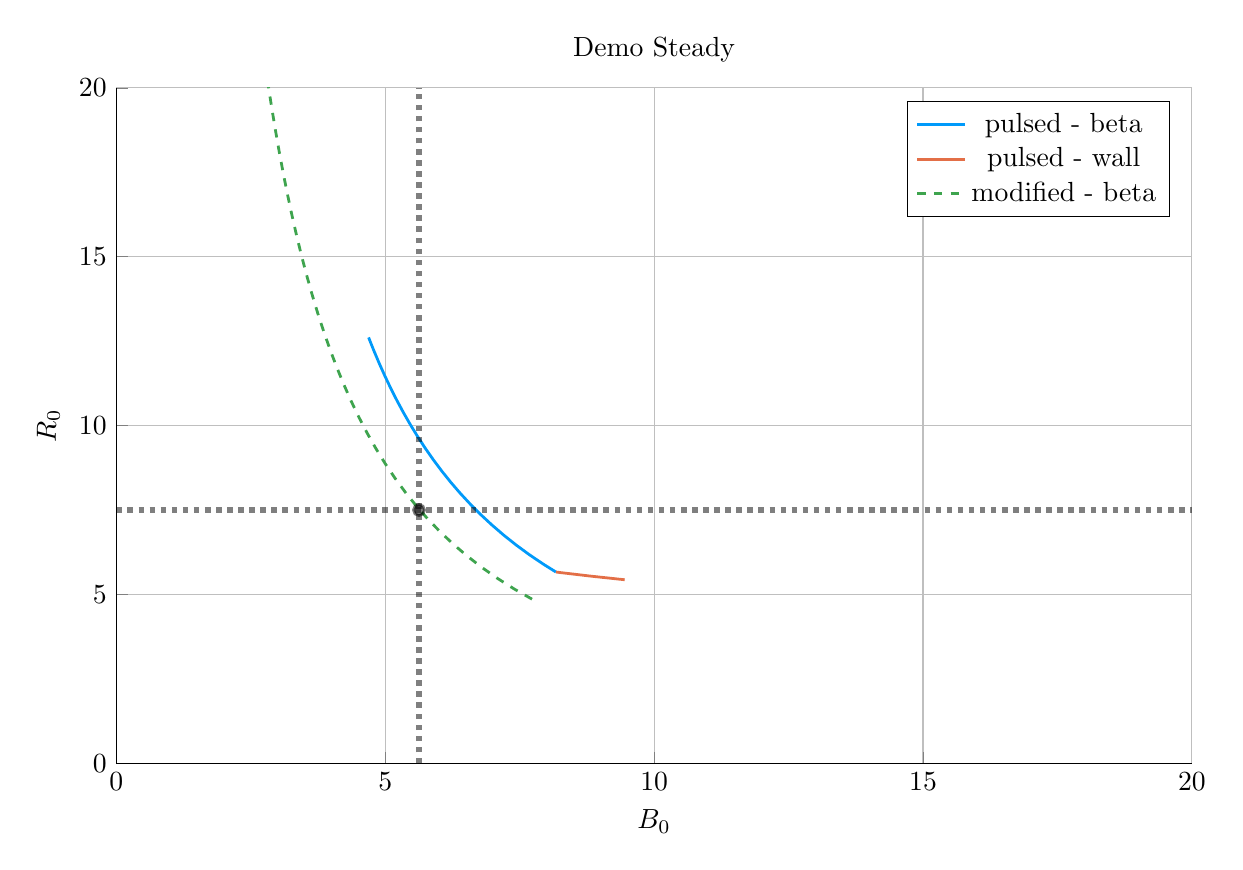
\begin{tikzpicture}[]
\begin{axis}[height = {101.6mm}, ylabel = {$R_0$}, title = {Demo Steady}, xmin = {0.0}, xmax = {20.0}, ymax = {20.0}, xlabel = {$B_0$}, {unbounded coords=jump, scaled x ticks = false, xticklabel style={rotate = 0}, xmajorgrids = true, xtick = {0.0,5.0,10.0,15.0,20.0}, xticklabels = {0,5,10,15,20}, xtick align = inside, axis lines* = left, scaled y ticks = false, yticklabel style={rotate = 0}, ymajorgrids = true, ytick = {0.0,5.0,10.0,15.0,20.0}, yticklabels = {0,5,10,15,20}, ytick align = inside, axis lines* = left,     xshift = 0.0mm,
    yshift = 0.0mm,
    axis background/.style={fill={rgb,1:red,1.00000000;green,1.00000000;blue,1.00000000}}
}, ymin = {0.0}, width = {152.4mm}]\addplot+ [color = {rgb,1:red,0.00000000;green,0.60560316;blue,0.97868012},
draw opacity=1.0,
line width=1,
solid,mark = none,
mark size = 2.0,
mark options = {
    color = {rgb,1:red,0.00000000;green,0.00000000;blue,0.00000000}, draw opacity = 1.0,
    fill = {rgb,1:red,0.00000000;green,0.60560316;blue,0.97868012}, fill opacity = 1.0,
    line width = 1,
    rotate = 0,
    solid
}]coordinates {
(8.173486873088942, 5.664794455960266)
(7.942780080136996, 5.894389477908349)
(7.682110747013332, 6.174587309854596)
(7.436076373351653, 6.4617259587740365)
(7.203701032854224, 6.7556817964635885)
(6.984087846006315, 7.056316762210614)
(6.776411507024863, 7.363478485110443)
(6.579911624110169, 7.677000456183209)
(6.393886772782909, 7.996702249919802)
(6.217689175869905, 8.322389794615686)
(6.050719935402341, 8.653855690575247)
(5.892424751644716, 8.990879574996331)
(5.742290072962272, 9.333228532083597)
(5.599839627496144, 9.680657546690735)
(5.464631293842628, 10.03290999955685)
(5.33625427328881, 10.389718201981736)
(5.214326530771975, 10.75080396758328)
(5.098492475718857, 11.115879218594692)
(4.98842085737482, 11.484646623994054)
(4.88380285223036, 11.85680026661456)
(4.784350323760147, 12.232026336259217)
(4.689794236961777, 12.610003845742904)
};
\addlegendentry{pulsed - beta}
\addplot+ [color = {rgb,1:red,0.88887350;green,0.43564919;blue,0.27812294},
draw opacity=1.0,
line width=1,
solid,mark = none,
mark size = 2.0,
mark options = {
    color = {rgb,1:red,0.00000000;green,0.00000000;blue,0.00000000}, draw opacity = 1.0,
    fill = {rgb,1:red,0.88887350;green,0.43564919;blue,0.27812294}, fill opacity = 1.0,
    line width = 1,
    rotate = 0,
    solid
}]coordinates {
(9.452194760190558, 5.436039445052516)
(8.82895875946862, 5.541751345019407)
(8.260410483462291, 5.64769543408014)
(8.173486873088942, 5.664794455960266)
};
\addlegendentry{pulsed - wall}
\addplot+ [color = {rgb,1:red,0.24222430;green,0.64327509;blue,0.30444865},
draw opacity=1.0,
line width=1,
dashed,mark = none,
mark size = 2.0,
mark options = {
    color = {rgb,1:red,0.00000000;green,0.00000000;blue,0.00000000}, draw opacity = 1.0,
    fill = {rgb,1:red,0.24222430;green,0.64327509;blue,0.30444865}, fill opacity = 1.0,
    line width = 1,
    rotate = 0,
    solid
}]coordinates {
(7.729015258613306, 4.861871150043874)
(7.398090906424027, 5.162615732748398)
(7.087604971989989, 5.475689582149146)
(6.796029845186129, 5.801261884855786)
(6.5219747916377235, 6.139486028413868)
(6.264171517105504, 6.490498735804173)
(6.021461495247516, 6.854419238072999)
(5.792784817023639, 7.231348485954994)
(5.57717035299729, 7.621368405021026)
(5.3737270519036775, 8.024541198865679)
(5.1816362256187425, 8.440908704652248)
(5.000144692923053, 8.870491805097014)
(4.828558673035444, 9.313289900712723)
(4.666238335465348, 9.769280445839089)
(4.512592925835539, 10.23841855166636)
(4.367076398389423, 10.720636659108127)
(4.229183495269078, 11.215844284001262)
(4.098446220614958, 11.723927836706606)
(3.974430664327246, 12.244750517759236)
(3.856734136133517, 12.778152290770123)
(3.744982575583214, 13.323949933321568)
(3.6388282078672565, 13.881937166125676)
(3.537947419047361, 14.45188486023713)
(3.4420388274654035, 15.033541321628862)
(3.3508215308612357, 15.626632651963563)
(3.2640335111230074, 16.230863183919308)
(3.18143018067718, 16.84591598897328)
(3.1027830563428513, 17.471453455103656)
(3.0278785480626333, 18.107117931452404)
(2.956516851312625, 18.752532436599008)
(2.888510933213844, 19.407301426734122)
(2.823685603439882, 20.071011619694055)
(2.761876661959762, 20.74323287052923)
(2.702930116488407, 21.423519094029906)
(2.646701463253573, 22.111409229427537)
(2.593055025340143, 22.806428242329144)
};
\addlegendentry{modified - beta}
\addplot+ [color = {rgb,1:red,0.00000000;green,0.00000000;blue,0.00000000},
draw opacity=0.5,
line width=2,
dotted,mark = none,
mark size = 2.0,
mark options = {
    color = {rgb,1:red,0.00000000;green,0.00000000;blue,0.00000000}, draw opacity = 0.5,
    fill = {rgb,1:red,0.00000000;green,0.00000000;blue,0.00000000}, fill opacity = 0.5,
    line width = 1,
    rotate = 0,
    solid
},forget plot]coordinates {
(0.0, 7.5)
(20.0, 7.5)
};
\addplot+ [color = {rgb,1:red,0.00000000;green,0.00000000;blue,0.00000000},
draw opacity=0.5,
line width=2,
dotted,mark = none,
mark size = 2.0,
mark options = {
    color = {rgb,1:red,0.00000000;green,0.00000000;blue,0.00000000}, draw opacity = 0.5,
    fill = {rgb,1:red,0.00000000;green,0.00000000;blue,0.00000000}, fill opacity = 0.5,
    line width = 1,
    rotate = 0,
    solid
},forget plot]coordinates {
(5.627, 0.0)
(5.627, 20.0)
};
\addplot+[draw=none, color = {rgb,1:red,0.00000000;green,0.00000000;blue,0.00000000},
draw opacity=0.5,
line width=0,
solid,mark = *,
mark size = 2.0,
mark options = {
    color = {rgb,1:red,0.00000000;green,0.00000000;blue,0.00000000}, draw opacity = 0.5,
    fill = {rgb,1:red,0.00000000;green,0.00000000;blue,0.00000000}, fill opacity = 0.5,
    line width = 1,
    rotate = 0,
    solid
},forget plot] coordinates {
(5.627, 7.5)
};
\end{axis}

\end{tikzpicture}

    \end{adjustbox}
        \caption{$R_0$ vs $B_0$}
    \end{subfigure}
    \hfill
    \begin{subfigure}[t]{0.45\textwidth}
        \centering
    \begin{adjustbox}{width=\textwidth}
      \Large
      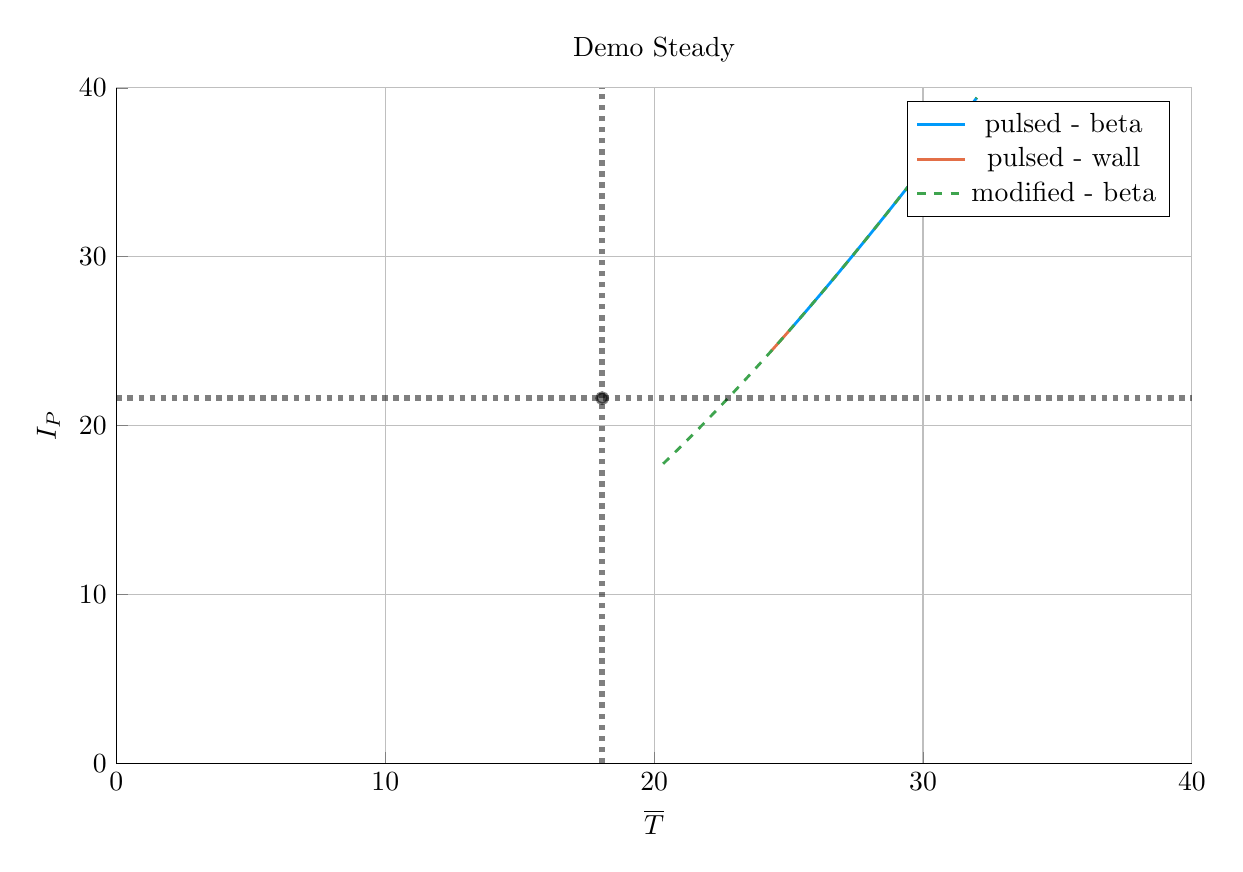
\begin{tikzpicture}[]
\begin{axis}[height = {101.6mm}, ylabel = {$I_P$}, title = {Demo Steady}, xmin = {0.0}, xmax = {40.0}, ymax = {40.0}, xlabel = {$\overline T$}, {unbounded coords=jump, scaled x ticks = false, xticklabel style={rotate = 0}, xmajorgrids = true, xtick = {0.0,10.0,20.0,30.0,40.0}, xticklabels = {0,10,20,30,40}, xtick align = inside, axis lines* = left, scaled y ticks = false, yticklabel style={rotate = 0}, ymajorgrids = true, ytick = {0.0,10.0,20.0,30.0,40.0}, yticklabels = {0,10,20,30,40}, ytick align = inside, axis lines* = left,     xshift = 0.0mm,
    yshift = 0.0mm,
    axis background/.style={fill={rgb,1:red,1.00000000;green,1.00000000;blue,1.00000000}}
}, ymin = {0.0}, width = {152.4mm}]\addplot+ [color = {rgb,1:red,0.00000000;green,0.60560316;blue,0.97868012},
draw opacity=1.0,
line width=1,
solid,mark = none,
mark size = 2.0,
mark options = {
    color = {rgb,1:red,0.00000000;green,0.00000000;blue,0.00000000}, draw opacity = 1.0,
    fill = {rgb,1:red,0.00000000;green,0.60560316;blue,0.97868012}, fill opacity = 1.0,
    line width = 1,
    rotate = 0,
    solid
}]coordinates {
(25.053735982163357, 25.677558860299992)
(25.333333333333332, 26.189593064380034)
(25.666666666666668, 26.80548085953921)
(26.0, 27.427148406840605)
(26.333333333333332, 28.054440831282633)
(26.666666666666668, 28.68719962041386)
(27.0, 29.325262818659787)
(27.333333333333332, 29.968465226287904)
(27.666666666666668, 30.6166386025962)
(28.0, 31.269611872884024)
(28.333333333333332, 31.92721133872904)
(28.666666666666668, 32.589260891064264)
(29.0, 33.25558222552837)
(29.333333333333332, 33.925995059549685)
(29.666666666666668, 34.60031735061725)
(30.0, 35.27836551518855)
(30.333333333333332, 35.95995464768734)
(30.666666666666668, 36.644898739049395)
(31.0, 37.333010894283476)
(31.333333333333332, 38.02410354852819)
(31.666666666666668, 38.717988681099214)
(32.0, 39.41447802704077)
};
\addlegendentry{pulsed - beta}
\addplot+ [color = {rgb,1:red,0.88887350;green,0.43564919;blue,0.27812294},
draw opacity=1.0,
line width=1,
solid,mark = none,
mark size = 2.0,
mark options = {
    color = {rgb,1:red,0.00000000;green,0.00000000;blue,0.00000000}, draw opacity = 1.0,
    fill = {rgb,1:red,0.88887350;green,0.43564919;blue,0.27812294}, fill opacity = 1.0,
    line width = 1,
    rotate = 0,
    solid
}]coordinates {
(24.333333333333332, 24.378107374495485)
(24.666666666666668, 24.975762903314084)
(25.0, 25.579637086786484)
(25.053735982163357, 25.677558860299992)
};
\addlegendentry{pulsed - wall}
\addplot+ [color = {rgb,1:red,0.24222430;green,0.64327509;blue,0.30444865},
draw opacity=1.0,
line width=1,
dashed,mark = none,
mark size = 2.0,
mark options = {
    color = {rgb,1:red,0.00000000;green,0.00000000;blue,0.00000000}, draw opacity = 1.0,
    fill = {rgb,1:red,0.24222430;green,0.64327509;blue,0.30444865}, fill opacity = 1.0,
    line width = 1,
    rotate = 0,
    solid
}]coordinates {
(20.333333333333332, 17.737142606162497)
(20.666666666666668, 18.250736761644205)
(21.0, 18.771889258341997)
(21.333333333333332, 19.300518519223587)
(21.666666666666668, 19.836537357082282)
(22.0, 20.37985305559639)
(22.333333333333332, 20.930367463801495)
(22.666666666666668, 21.487977099646507)
(23.0, 22.05257326267931)
(23.333333333333332, 22.62404215595106)
(23.666666666666668, 23.202265017123075)
(24.0, 23.787118258664318)
(24.333333333333332, 24.378473616949)
(24.666666666666668, 24.976198309995638)
(25.0, 25.58015520352756)
(25.333333333333332, 26.19020298497985)
(25.666666666666668, 26.806196345025047)
(26.0, 27.427986166140983)
(26.333333333333332, 28.055419717698932)
(26.666666666666668, 28.688340857006587)
(27.0, 29.3265902357016)
(27.333333333333332, 29.970005510854897)
(27.666666666666668, 30.61842156011136)
(28.0, 31.27167070016686)
(28.333333333333332, 31.92958290785876)
(28.666666666666668, 32.591986043126525)
(29.0, 33.25870607308836)
(29.333333333333332, 33.929567296470175)
(29.666666666666668, 34.604392567622554)
(30.0, 35.28300351936469)
(30.333333333333332, 35.96522078390488)
(30.666666666666668, 36.650864211102025)
(31.0, 37.3397530833557)
(31.333333333333332, 38.03170632643894)
(31.666666666666668, 38.726542715621264)
(32.0, 39.424081076468326)
};
\addlegendentry{modified - beta}
\addplot+ [color = {rgb,1:red,0.00000000;green,0.00000000;blue,0.00000000},
draw opacity=0.5,
line width=2,
dotted,mark = none,
mark size = 2.0,
mark options = {
    color = {rgb,1:red,0.00000000;green,0.00000000;blue,0.00000000}, draw opacity = 0.5,
    fill = {rgb,1:red,0.00000000;green,0.00000000;blue,0.00000000}, fill opacity = 0.5,
    line width = 1,
    rotate = 0,
    solid
},forget plot]coordinates {
(0.0, 21.627)
(40.0, 21.627)
};
\addplot+ [color = {rgb,1:red,0.00000000;green,0.00000000;blue,0.00000000},
draw opacity=0.5,
line width=2,
dotted,mark = none,
mark size = 2.0,
mark options = {
    color = {rgb,1:red,0.00000000;green,0.00000000;blue,0.00000000}, draw opacity = 0.5,
    fill = {rgb,1:red,0.00000000;green,0.00000000;blue,0.00000000}, fill opacity = 0.5,
    line width = 1,
    rotate = 0,
    solid
},forget plot]coordinates {
(18.067, 0.0)
(18.067, 40.0)
};
\addplot+[draw=none, color = {rgb,1:red,0.00000000;green,0.00000000;blue,0.00000000},
draw opacity=0.5,
line width=0,
solid,mark = *,
mark size = 2.0,
mark options = {
    color = {rgb,1:red,0.00000000;green,0.00000000;blue,0.00000000}, draw opacity = 0.5,
    fill = {rgb,1:red,0.00000000;green,0.00000000;blue,0.00000000}, fill opacity = 0.5,
    line width = 1,
    rotate = 0,
    solid
},forget plot] coordinates {
(18.067, 21.627)
};
\end{axis}

\end{tikzpicture}

    \end{adjustbox}
        \caption{$I_P$ vs $\overline T$}
    \end{subfigure}
    \hfill \hfill ~\\ ~\\ ~\\
    \caption{Demo Steady Model Comparison} ~\\
\end{figure*}

\begin{table}[h!]
\centering  
\caption{Demo Steady Variables}
\hfill
\begin{subtable}[t]{0.4\textwidth}
\centering  
\caption{Input Variables} ~\\
\begin{tabular}{ c|c } 

Input            & Value           \\
\hline
$H$              & 1.4             \\
$Q$              & 24.46           \\
$N_{G}$          & 1.2             \\
$\epsilon$       & 0.385           \\
$\kappa_{95}$    & 1.8             \\
$\delta_{95}$    & 0.333           \\
$\nu_{n}$        & 0.3972          \\
$\nu_{T}$        & 0.9187          \\
$l_{i}$          & 0.9             \\
$A$              & 2.856           \\
$Z_{eff}$        & 4.708           \\
$f_{D}$          & 0.7366          \\
$\tau_{FT}$      & 1.6e9           \\
$B_{CS}$         & 12.85           \\

\end{tabular}
\end{subtable}
\hfill
\begin{subtable}[t]{0.5\textwidth}
\centering  
\caption{Output Variables} ~\\
\begin{tabular}{ c|c|c } 

Output           & Original         & Fussy.jl        \\  
\hline
$R_{0}$          & 7.5              & 8.154           \\
$B_{0}$          & 5.627            & 6.307           \\
$I_{P}$          & 21.63            & 30.93           \\
$\overline n$    & 0.8746           & 1.048           \\
$\overline T$    & 18.07            & 27.83           \\
$\beta_{N}$       & 0.038            & 0.038           \\
$q_{95}$         & 4.405            & 3.761           \\
$P_{W}$          & 1.911            & 4.151           \\
$f_{BS}$         & 0.611            & 0.4241          \\
$f_{CD}$         & 0.389            & 0.5759          \\
$f_{IN}$         & -              & -             \\
$\volume$         & 2217           & 2879          \\
$P_{F}$          & 3255           & 8971          \\
$\eta_{CD}$      & 0.4152           & -          \\

\end{tabular}
\end{subtable}
\hfill
\hfill
\end{table}

\newpage 

\subsubsection{DEMO Pulsed -- A Pulsed ITER Successor}

\begin{figure*}[h!]
    \centering
    \hfill 
    \begin{subfigure}[t]{0.45\textwidth}
        \centering
    \begin{adjustbox}{width=\textwidth}
      \Large
      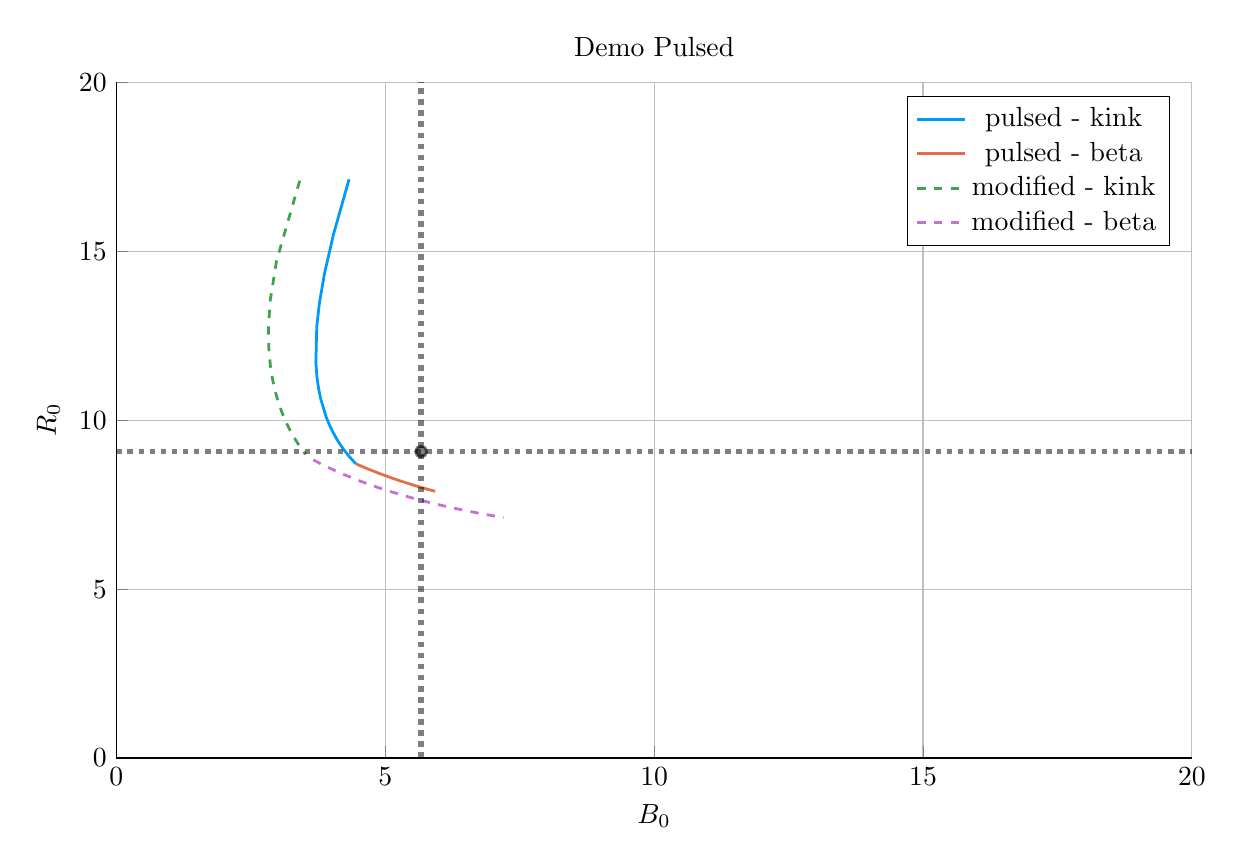
\begin{tikzpicture}[]
\begin{axis}[height = {101.6mm}, ylabel = {$R_0$}, title = {Demo Pulsed}, xmin = {0.0}, xmax = {20.0}, ymax = {20.0}, xlabel = {$B_0$}, {unbounded coords=jump, scaled x ticks = false, xticklabel style={rotate = 0}, xmajorgrids = true, xtick = {0.0,5.0,10.0,15.0,20.0}, xticklabels = {0,5,10,15,20}, xtick align = inside, axis lines* = left, scaled y ticks = false, yticklabel style={rotate = 0}, ymajorgrids = true, ytick = {0.0,5.0,10.0,15.0,20.0}, yticklabels = {0,5,10,15,20}, ytick align = inside, axis lines* = left,     xshift = 0.0mm,
    yshift = 0.0mm,
    axis background/.style={fill={rgb,1:red,1.00000000;green,1.00000000;blue,1.00000000}}
}, ymin = {0.0}, width = {152.4mm}]\addplot+ [color = {rgb,1:red,0.00000000;green,0.60560316;blue,0.97868012},
draw opacity=1.0,
line width=1,
solid,mark = none,
mark size = 2.0,
mark options = {
    color = {rgb,1:red,0.00000000;green,0.00000000;blue,0.00000000}, draw opacity = 1.0,
    fill = {rgb,1:red,0.00000000;green,0.60560316;blue,0.97868012}, fill opacity = 1.0,
    line width = 1,
    rotate = 0,
    solid
}]coordinates {
(4.327031075670194, 17.134796748649162)
(4.038214026054326, 15.511755022601415)
(3.8713719163129245, 14.355562963913712)
(3.7758613845615545, 13.476675762289453)
(3.7257856761317214, 12.778294295391971)
(3.7090473695925437, 11.723065749829066)
(3.727711597554826, 11.30970201784727)
(3.7586131667481433, 10.94971275897184)
(3.799052518631718, 10.632190690377048)
(3.901290136389271, 10.09455415135144)
(3.960577465316514, 9.863813619410237)
(4.0241209645210345, 9.653307397969705)
(4.0912717805663785, 9.460162902699798)
(4.161514602943343, 9.28206292757184)
(4.2344343960723005, 9.117114543572253)
(4.309692554546368, 8.963753917462126)
(4.450417240491067, 8.712493965092264)
};
\addlegendentry{pulsed - kink}
\addplot+ [color = {rgb,1:red,0.88887350;green,0.43564919;blue,0.27812294},
draw opacity=1.0,
line width=1,
solid,mark = none,
mark size = 2.0,
mark options = {
    color = {rgb,1:red,0.00000000;green,0.00000000;blue,0.00000000}, draw opacity = 1.0,
    fill = {rgb,1:red,0.88887350;green,0.43564919;blue,0.27812294}, fill opacity = 1.0,
    line width = 1,
    rotate = 0,
    solid
}]coordinates {
(4.450417240491067, 8.712493965092264)
(4.490148631384312, 8.684308742646298)
(4.692490181445514, 8.547262773806349)
(4.8960344619053355, 8.41947837460442)
(5.100651132702229, 8.30014929484307)
(5.306202822090688, 8.188581738801314)
(5.512545696627038, 8.084175191078112)
(5.719530043226767, 7.986407002697611)
(5.927000883375481, 7.894819882619234)
};
\addlegendentry{pulsed - beta}
\addplot+ [color = {rgb,1:red,0.24222430;green,0.64327509;blue,0.30444865},
draw opacity=1.0,
line width=1,
dashed,mark = none,
mark size = 2.0,
mark options = {
    color = {rgb,1:red,0.00000000;green,0.00000000;blue,0.00000000}, draw opacity = 1.0,
    fill = {rgb,1:red,0.24222430;green,0.64327509;blue,0.30444865}, fill opacity = 1.0,
    line width = 1,
    rotate = 0,
    solid
}]coordinates {
(3.4087424183072135, 17.090884129081292)
(2.977074181068944, 14.713048632784332)
(2.8592500074202523, 13.541171522519205)
(2.827199220063259, 12.740024138753894)
(2.8339789008667826, 12.12574468151967)
(2.862412302880871, 11.626187613249266)
(2.9044598258085443, 11.205091848948229)
(2.95577893007882, 10.841432203317366)
(3.0137895352525907, 10.521822649209419)
(3.076849710218805, 10.23716073884787)
(3.1438583711612704, 9.980947801083442)
(3.214045733980633, 9.748367275345563)
(3.2868548955983727, 9.535742205343247)
(3.361871149981842, 9.340197658526863)
(3.4387778750377818, 9.15944098345979)
(3.5173279629378453, 8.991613349767409)
};
\addlegendentry{modified - kink}
\addplot+ [color = {rgb,1:red,0.76444018;green,0.44411178;blue,0.82429754},
draw opacity=1.0,
line width=1,
dashed,mark = none,
mark size = 2.0,
mark options = {
    color = {rgb,1:red,0.00000000;green,0.00000000;blue,0.00000000}, draw opacity = 1.0,
    fill = {rgb,1:red,0.76444018;green,0.44411178;blue,0.82429754}, fill opacity = 1.0,
    line width = 1,
    rotate = 0,
    solid
}]coordinates {
(3.6607028750648505, 8.825949645171955)
(3.8574448036470477, 8.664618827122876)
(4.056375867871351, 8.51434867582932)
(4.257366397480293, 8.374075613831488)
(4.460279103534801, 8.242896218794312)
(4.664969389370631, 8.12003771613466)
(4.871285596007394, 8.004834914067093)
(5.07906923307514, 7.896711937521184)
(5.288155233306219, 7.795167587687744)
(5.498372259673351, 7.699763475973523)
(5.709543087166185, 7.610114306522102)
(5.921485076209294, 7.525879840414137)
(6.134010749367255, 7.446758190646709)
(6.346928478632384, 7.372480180910637)
(6.560043285872518, 7.302804563889649)
(6.773157754368795, 7.237513941672651)
(6.986073044284746, 7.176411266758267)
(7.198590001107076, 7.119316828230052)
};
\addlegendentry{modified - beta}
\addplot+ [color = {rgb,1:red,0.00000000;green,0.00000000;blue,0.00000000},
draw opacity=0.5,
line width=2,
dotted,mark = none,
mark size = 2.0,
mark options = {
    color = {rgb,1:red,0.00000000;green,0.00000000;blue,0.00000000}, draw opacity = 0.5,
    fill = {rgb,1:red,0.00000000;green,0.00000000;blue,0.00000000}, fill opacity = 0.5,
    line width = 1,
    rotate = 0,
    solid
},forget plot]coordinates {
(0.0, 9.072)
(20.0, 9.072)
};
\addplot+ [color = {rgb,1:red,0.00000000;green,0.00000000;blue,0.00000000},
draw opacity=0.5,
line width=2,
dotted,mark = none,
mark size = 2.0,
mark options = {
    color = {rgb,1:red,0.00000000;green,0.00000000;blue,0.00000000}, draw opacity = 0.5,
    fill = {rgb,1:red,0.00000000;green,0.00000000;blue,0.00000000}, fill opacity = 0.5,
    line width = 1,
    rotate = 0,
    solid
},forget plot]coordinates {
(5.667, 0.0)
(5.667, 20.0)
};
\addplot+[draw=none, color = {rgb,1:red,0.00000000;green,0.00000000;blue,0.00000000},
draw opacity=0.5,
line width=0,
solid,mark = *,
mark size = 2.0,
mark options = {
    color = {rgb,1:red,0.00000000;green,0.00000000;blue,0.00000000}, draw opacity = 0.5,
    fill = {rgb,1:red,0.00000000;green,0.00000000;blue,0.00000000}, fill opacity = 0.5,
    line width = 1,
    rotate = 0,
    solid
},forget plot] coordinates {
(5.667, 9.072)
};
\end{axis}

\end{tikzpicture}

    \end{adjustbox}
        \caption{$R_0$ vs $B_0$}
    \end{subfigure}
    \hfill
    \begin{subfigure}[t]{0.45\textwidth}
        \centering
    \begin{adjustbox}{width=\textwidth}
      \Large
      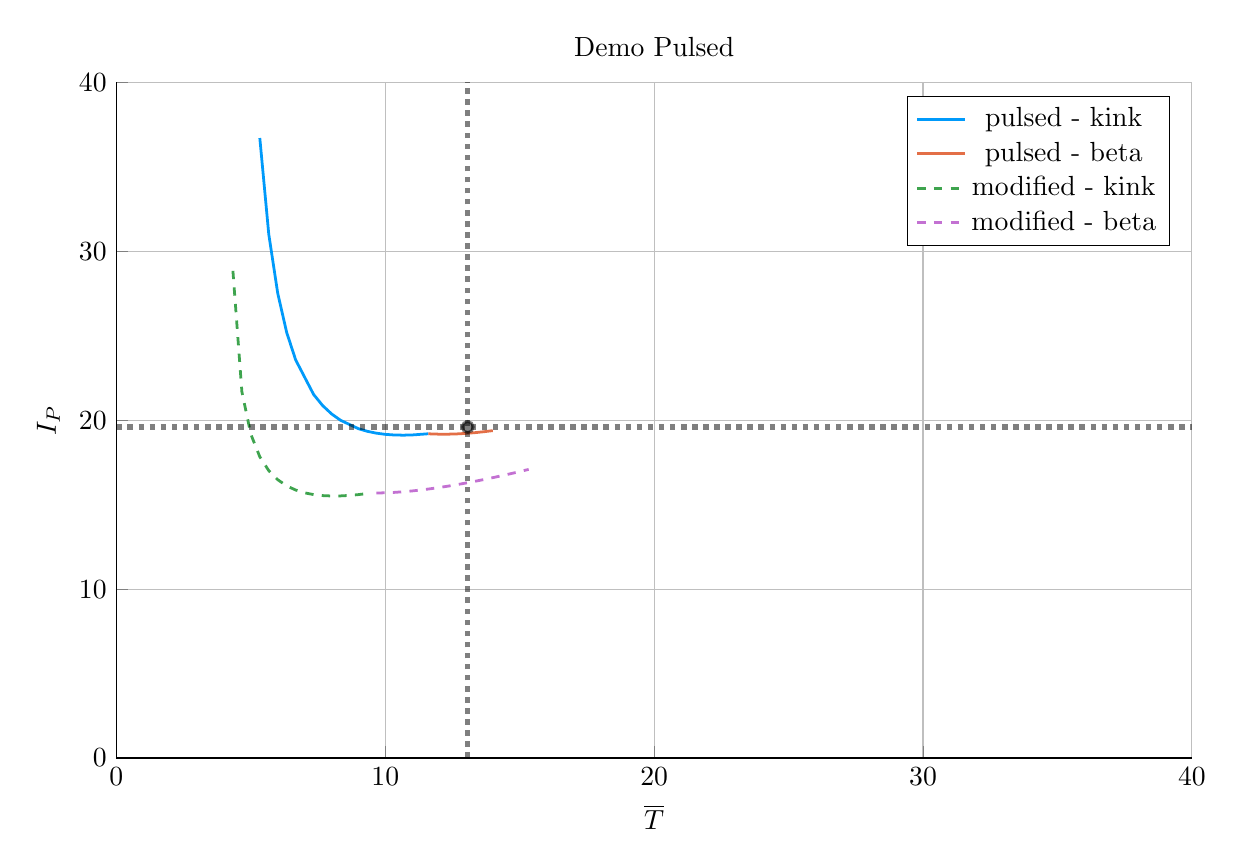
\begin{tikzpicture}[]
\begin{axis}[height = {101.6mm}, ylabel = {$I_P$}, title = {Demo Pulsed}, xmin = {0.0}, xmax = {40.0}, ymax = {40.0}, xlabel = {$\overline T$}, {unbounded coords=jump, scaled x ticks = false, xticklabel style={rotate = 0}, xmajorgrids = true, xtick = {0.0,10.0,20.0,30.0,40.0}, xticklabels = {0,10,20,30,40}, xtick align = inside, axis lines* = left, scaled y ticks = false, yticklabel style={rotate = 0}, ymajorgrids = true, ytick = {0.0,10.0,20.0,30.0,40.0}, yticklabels = {0,10,20,30,40}, ytick align = inside, axis lines* = left,     xshift = 0.0mm,
    yshift = 0.0mm,
    axis background/.style={fill={rgb,1:red,1.00000000;green,1.00000000;blue,1.00000000}}
}, ymin = {0.0}, width = {152.4mm}]\addplot+ [color = {rgb,1:red,0.00000000;green,0.60560316;blue,0.97868012},
draw opacity=1.0,
line width=1,
solid,mark = none,
mark size = 2.0,
mark options = {
    color = {rgb,1:red,0.00000000;green,0.00000000;blue,0.00000000}, draw opacity = 1.0,
    fill = {rgb,1:red,0.00000000;green,0.60560316;blue,0.97868012}, fill opacity = 1.0,
    line width = 1,
    rotate = 0,
    solid
}]coordinates {
(5.333333333333333, 36.71051032912112)
(5.666666666666667, 31.014995367356207)
(6.0, 27.51734786322149)
(6.333333333333333, 25.19534286389616)
(6.666666666666667, 23.57285610926683)
(7.333333333333333, 21.52905816503197)
(7.666666666666667, 20.874444053021588)
(8.0, 20.377542510464334)
(8.333333333333334, 19.99951688957442)
(9.0, 19.499202175706746)
(9.333333333333334, 19.343044014643887)
(9.666666666666666, 19.233955791269285)
(10.0, 19.16365729524907)
(10.333333333333334, 19.125701869840853)
(10.666666666666666, 19.11499858904485)
(11.0, 19.127475979338943)
(11.600962879632572, 19.198383823705257)
};
\addlegendentry{pulsed - kink}
\addplot+ [color = {rgb,1:red,0.88887350;green,0.43564919;blue,0.27812294},
draw opacity=1.0,
line width=1,
solid,mark = none,
mark size = 2.0,
mark options = {
    color = {rgb,1:red,0.00000000;green,0.00000000;blue,0.00000000}, draw opacity = 1.0,
    fill = {rgb,1:red,0.88887350;green,0.43564919;blue,0.27812294}, fill opacity = 1.0,
    line width = 1,
    rotate = 0,
    solid
}]coordinates {
(11.600962879632572, 19.198383823705257)
(11.666666666666666, 19.192414153878335)
(12.0, 19.174087186739918)
(12.333333333333334, 19.17397121853779)
(12.666666666666666, 19.189978018951553)
(13.0, 19.220357277326283)
(13.333333333333334, 19.263633100211838)
(13.666666666666666, 19.31855421750887)
(14.0, 19.384054548489104)
};
\addlegendentry{pulsed - beta}
\addplot+ [color = {rgb,1:red,0.24222430;green,0.64327509;blue,0.30444865},
draw opacity=1.0,
line width=1,
dashed,mark = none,
mark size = 2.0,
mark options = {
    color = {rgb,1:red,0.00000000;green,0.00000000;blue,0.00000000}, draw opacity = 1.0,
    fill = {rgb,1:red,0.24222430;green,0.64327509;blue,0.30444865}, fill opacity = 1.0,
    line width = 1,
    rotate = 0,
    solid
}]coordinates {
(4.333333333333333, 28.845639077165217)
(4.666666666666667, 21.687713986294685)
(5.0, 19.170340224057398)
(5.333333333333333, 17.83397336320386)
(5.666666666666667, 17.01478565989059)
(6.0, 16.477486603636205)
(6.333333333333333, 16.113958654578386)
(6.666666666666667, 15.866460603971907)
(7.0, 15.700928946757587)
(7.333333333333333, 15.59578560596909)
(7.666666666666667, 15.536607983152381)
(8.0, 15.513342675582972)
(8.333333333333334, 15.518740955012225)
(8.666666666666666, 15.547428978968492)
(9.0, 15.595329068459918)
(9.333333333333334, 15.659285368310089)
};
\addlegendentry{modified - kink}
\addplot+ [color = {rgb,1:red,0.76444018;green,0.44411178;blue,0.82429754},
draw opacity=1.0,
line width=1,
dashed,mark = none,
mark size = 2.0,
mark options = {
    color = {rgb,1:red,0.00000000;green,0.00000000;blue,0.00000000}, draw opacity = 1.0,
    fill = {rgb,1:red,0.76444018;green,0.44411178;blue,0.82429754}, fill opacity = 1.0,
    line width = 1,
    rotate = 0,
    solid
}]coordinates {
(9.666666666666666, 15.691192911261952)
(10.0, 15.70165788278533)
(10.333333333333334, 15.726578234093749)
(10.666666666666666, 15.764127054896537)
(11.0, 15.812802650736373)
(11.333333333333334, 15.871360766004056)
(11.666666666666666, 15.938763317563621)
(12.0, 16.014139065408)
(12.333333333333334, 16.09675304572932)
(12.666666666666666, 16.185982524147033)
(13.0, 16.281297862810217)
(13.333333333333334, 16.382247130746602)
(13.666666666666666, 16.488443597982137)
(14.0, 16.5995554722192)
(14.333333333333334, 16.715297396529092)
(14.666666666666666, 16.83542334285969)
(15.0, 16.959720624053933)
(15.333333333333334, 17.088004807739882)
};
\addlegendentry{modified - beta}
\addplot+ [color = {rgb,1:red,0.00000000;green,0.00000000;blue,0.00000000},
draw opacity=0.5,
line width=2,
dotted,mark = none,
mark size = 2.0,
mark options = {
    color = {rgb,1:red,0.00000000;green,0.00000000;blue,0.00000000}, draw opacity = 0.5,
    fill = {rgb,1:red,0.00000000;green,0.00000000;blue,0.00000000}, fill opacity = 0.5,
    line width = 1,
    rotate = 0,
    solid
},forget plot]coordinates {
(0.0, 19.6)
(40.0, 19.6)
};
\addplot+ [color = {rgb,1:red,0.00000000;green,0.00000000;blue,0.00000000},
draw opacity=0.5,
line width=2,
dotted,mark = none,
mark size = 2.0,
mark options = {
    color = {rgb,1:red,0.00000000;green,0.00000000;blue,0.00000000}, draw opacity = 0.5,
    fill = {rgb,1:red,0.00000000;green,0.00000000;blue,0.00000000}, fill opacity = 0.5,
    line width = 1,
    rotate = 0,
    solid
},forget plot]coordinates {
(13.065, 0.0)
(13.065, 40.0)
};
\addplot+[draw=none, color = {rgb,1:red,0.00000000;green,0.00000000;blue,0.00000000},
draw opacity=0.5,
line width=0,
solid,mark = *,
mark size = 2.0,
mark options = {
    color = {rgb,1:red,0.00000000;green,0.00000000;blue,0.00000000}, draw opacity = 0.5,
    fill = {rgb,1:red,0.00000000;green,0.00000000;blue,0.00000000}, fill opacity = 0.5,
    line width = 1,
    rotate = 0,
    solid
},forget plot] coordinates {
(13.065, 19.6)
};
\end{axis}

\end{tikzpicture}

    \end{adjustbox}
        \caption{$I_P$ vs $\overline T$}
    \end{subfigure}
    \hfill \hfill ~\\ ~\\ ~\\
    \caption{Demo Pulsed Model Comparison} ~\\
\end{figure*}

\begin{table}[h!]
\centering  
\caption{Demo Pulsed Variables}
\hfill
\begin{subtable}[t]{0.4\textwidth}
\centering  
\caption{Input Variables} ~\\
\begin{tabular}{ c|c } 

Input            & Value           \\
\hline
$H$              & 1.1             \\
$Q$              & 39.86           \\
$N_{G}$          & 1.2             \\
$\epsilon$       & 0.3226          \\
$\kappa_{95}$    & 1.59            \\
$\delta_{95}$    & 0.333           \\
$\nu_{n}$        & 0.27            \\
$\nu_{T}$        & 1.094           \\
$l_{i}$          & 1.155           \\
$A$              & 2.735           \\
$Z_{eff}$        & 2.584           \\
$f_{D}$          & 0.7753          \\
$\tau_{FT}$      & 7273          \\
$B_{CS}$         & 12.77           \\

\end{tabular}
\end{subtable}
\hfill
\begin{subtable}[t]{0.5\textwidth}
\centering  
\caption{Output Variables} ~\\
\begin{tabular}{ c|c|c } 

Output           & Original         & Fussy.jl        \\
\hline
$R_{0}$          & 9.072            & 8.1             \\
$B_{0}$          & 5.667            & 5.48            \\
$I_{P}$          & 19.6             & 19.26           \\
$\overline n$    & 0.7983           & 0.9795          \\
$\overline T$    & 13.06            & 13.28           \\
$\beta_{N}$       & 0.0259           & 0.0259          \\
$q_{95}$         & 3.247            & 2.853           \\
$P_{W}$          & 1.05             & 1.466           \\
$f_{BS}$         & 0.348            & 0.1637          \\
$f_{CD}$         & 0.096            & 0.1062          \\
$f_{IN}$         & 0.557            & 0.7302          \\
$\volume$         & 2502           & 1751          \\
$P_{F}$          & 2037           & 2376          \\
$\eta_{CD}$      & 0.2721           & -     

\end{tabular}
\end{subtable}
\hfill
\hfill
\end{table}

\section{Developing Prototype Reactors}

\begin{figure}[h!]
\centering
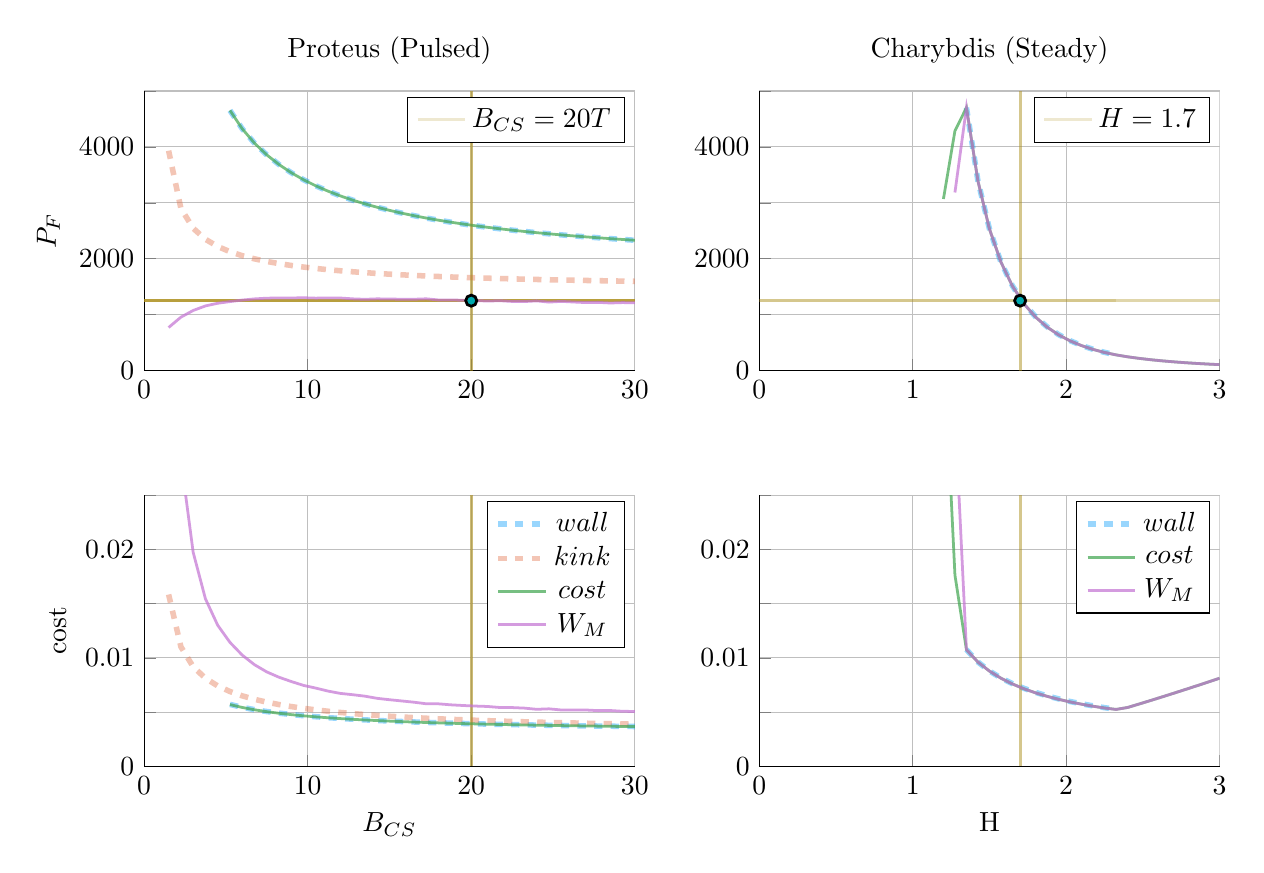
\begin{tikzpicture}[]
\begin{axis}[height = {51.32916666666667mm}, ylabel = {$P_F$}, title = {Proteus (Pulsed)}, xmin = {0}, xmax = {30.0}, ymax = {5000.0}, xlabel = {}, {unbounded coords=jump, scaled x ticks = false, xticklabel style={rotate = 0}, xmajorgrids = true, xtick = {0.0,10.0,20.0,30.0}, xticklabels = {0,10,20,30}, xtick align = inside, axis lines* = left, scaled y ticks = false, yticklabel style={rotate = 0}, ymajorgrids = true, ytick = {0,1000,2000,3000,4000,5000}, yticklabels = {0,,2000,,4000,}, ytick align = inside, axis lines* = left,     xshift = 0.0mm,
    yshift = 50.27mm,
    axis background/.style={fill={rgb,1:red,1.00000000;green,1.00000000;blue,1.00000000}}
}, ymin = {2.220446049250313e-16}, width = {78.14027777777778mm}]\addplot+ [color = {rgb,1:red,0.67554396;green,0.55566233;blue,0.09423434},
draw opacity=0.2,
line width=1,
solid,mark = none,
mark size = 2.0,
mark options = {
    color = {rgb,1:red,0.00000000;green,0.00000000;blue,0.00000000}, draw opacity = 1.0,
    fill = {rgb,1:red,0.67554396;green,0.55566233;blue,0.09423434}, fill opacity = 1.0,
    line width = 1,
    rotate = 0,
    solid
}]coordinates {
(20.0, 2.220446049250313e-16)
(20.0, 5000.0)
};
\addlegendentry{$B_{CS} = 20 T$}
\addplot+ [color = {rgb,1:red,0.67554396;green,0.55566233;blue,0.09423434},
draw opacity=0.2,
line width=1,
solid,mark = none,
mark size = 2.0,
mark options = {
    color = {rgb,1:red,0.00000000;green,0.00000000;blue,0.00000000}, draw opacity = 1.0,
    fill = {rgb,1:red,0.67554396;green,0.55566233;blue,0.09423434}, fill opacity = 1.0,
    line width = 1,
    rotate = 0,
    solid
},forget plot]coordinates {
(0.0, 1250.0)
(30.0, 1250.0)
};
\addplot+[draw=none, color = {rgb,1:red,0.00000048;green,0.66575898;blue,0.68099695},
draw opacity=1.0,
line width=0,
solid,mark = *,
mark size = 2.0,
mark options = {
    color = {rgb,1:red,0.00000000;green,0.00000000;blue,0.00000000}, draw opacity = 1.0,
    fill = {rgb,1:red,0.00000048;green,0.66575898;blue,0.68099695}, fill opacity = 1.0,
    line width = 1,
    rotate = 0,
    solid
},forget plot] coordinates {
(20, 1250)
};
\addplot+ [color = {rgb,1:red,0.67554396;green,0.55566233;blue,0.09423434},
draw opacity=0.2,
line width=1,
solid,mark = none,
mark size = 2.0,
mark options = {
    color = {rgb,1:red,0.00000000;green,0.00000000;blue,0.00000000}, draw opacity = 1.0,
    fill = {rgb,1:red,0.67554396;green,0.55566233;blue,0.09423434}, fill opacity = 1.0,
    line width = 1,
    rotate = 0,
    solid
},forget plot]coordinates {
(0.0, 1250.0)
(30.0, 1250.0)
};
\addplot+ [color = {rgb,1:red,0.00000000;green,0.60560316;blue,0.97868012},
draw opacity=0.4,
line width=2,
dashed,mark = none,
mark size = 2.0,
mark options = {
    color = {rgb,1:red,0.00000000;green,0.00000000;blue,0.00000000}, draw opacity = 1.0,
    fill = {rgb,1:red,0.00000000;green,0.60560316;blue,0.97868012}, fill opacity = 1.0,
    line width = 1,
    rotate = 0,
    solid
},forget plot]coordinates {
(5.25, 4651.734735476011)
(6.0, 4323.6250098364)
(6.75, 4065.99692078527)
(7.5, 3857.273578687972)
(8.25, 3684.1342593418663)
(9.0, 3537.844669896544)
(9.75, 3412.404653539425)
(10.5, 3303.536032694244)
(11.25, 3208.094051273514)
(12.0, 3123.707522754923)
(12.75, 3048.5495054628623)
(13.5, 2981.185980181023)
(14.25, 2920.472987010462)
(15.0, 2865.484885250518)
(15.75, 2815.463186166668)
(16.5, 2769.7793320244814)
(17.25, 2727.9071420752607)
(18.0, 2689.4020933235493)
(18.75, 2653.885520176901)
(19.5, 2621.0324111911764)
(20.25, 2590.561874678777)
(21.0, 2562.2296107375955)
(21.75, 2535.8219099446264)
(22.5, 2511.150826555893)
(23.25, 2488.050264495335)
(24.0, 2466.372779394113)
(24.75, 2445.986947213969)
(25.5, 2426.775184780072)
(26.25, 2408.6319334297787)
(27.0, 2391.4621364565396)
(27.75, 2375.1799557182867)
(28.5, 2359.707684182671)
(29.25, 2344.974819785335)
(30.0, 2330.917272823136)
};
\addplot+ [color = {rgb,1:red,0.67554396;green,0.55566233;blue,0.09423434},
draw opacity=0.2,
line width=1,
solid,mark = none,
mark size = 2.0,
mark options = {
    color = {rgb,1:red,0.00000000;green,0.00000000;blue,0.00000000}, draw opacity = 1.0,
    fill = {rgb,1:red,0.67554396;green,0.55566233;blue,0.09423434}, fill opacity = 1.0,
    line width = 1,
    rotate = 0,
    solid
},forget plot]coordinates {
(20.0, 2.220446049250313e-16)
(20.0, 5000.0)
};
\addplot+ [color = {rgb,1:red,0.67554396;green,0.55566233;blue,0.09423434},
draw opacity=0.2,
line width=1,
solid,mark = none,
mark size = 2.0,
mark options = {
    color = {rgb,1:red,0.00000000;green,0.00000000;blue,0.00000000}, draw opacity = 1.0,
    fill = {rgb,1:red,0.67554396;green,0.55566233;blue,0.09423434}, fill opacity = 1.0,
    line width = 1,
    rotate = 0,
    solid
},forget plot]coordinates {
(0.0, 1250.0)
(30.0, 1250.0)
};
\addplot+ [color = {rgb,1:red,0.67554396;green,0.55566233;blue,0.09423434},
draw opacity=0.2,
line width=1,
solid,mark = none,
mark size = 2.0,
mark options = {
    color = {rgb,1:red,0.00000000;green,0.00000000;blue,0.00000000}, draw opacity = 1.0,
    fill = {rgb,1:red,0.67554396;green,0.55566233;blue,0.09423434}, fill opacity = 1.0,
    line width = 1,
    rotate = 0,
    solid
},forget plot]coordinates {
(0.0, 1250.0)
(30.0, 1250.0)
};
\addplot+ [color = {rgb,1:red,0.88887350;green,0.43564919;blue,0.27812294},
draw opacity=0.4,
line width=2,
dashed,mark = none,
mark size = 2.0,
mark options = {
    color = {rgb,1:red,0.00000000;green,0.00000000;blue,0.00000000}, draw opacity = 1.0,
    fill = {rgb,1:red,0.88887350;green,0.43564919;blue,0.27812294}, fill opacity = 1.0,
    line width = 1,
    rotate = 0,
    solid
},forget plot]coordinates {
(1.5, 3931.6170696070676)
(2.25, 2900.7235747979908)
(3.0, 2544.8446560898715)
(3.75, 2348.228116500571)
(4.5, 2219.0134794713767)
(5.25, 2125.815532966674)
(6.0, 2054.566085735622)
(6.75, 1997.8824990557177)
(7.5, 1951.4633680592258)
(8.25, 1912.6074536455505)
(9.0, 1879.5196356674505)
(9.75, 1850.953068441656)
(10.5, 1826.0101459658863)
(11.25, 1804.02551415983)
(12.0, 1784.493638745381)
(12.75, 1767.0222758941622)
(13.5, 1751.3015387280175)
(14.25, 1737.0827328069474)
(15.0, 1724.1634044428295)
(15.75, 1712.376890482151)
(16.5, 1701.5841921715175)
(17.25, 1691.6685698179294)
(18.0, 1682.530881991843)
(18.75, 1674.0861755860074)
(19.5, 1666.2615100001372)
(20.25, 1658.9932835127363)
(21.0, 1652.2262595201232)
(21.75, 1645.91179207308)
(22.5, 1640.0070406407558)
(23.25, 1634.4738680952948)
(24.0, 1629.2785569006053)
(24.75, 1624.3908184475338)
(25.5, 1619.7835209277835)
(26.25, 1615.432247074283)
(27.0, 1611.314956936522)
(27.75, 1607.4117026157203)
(28.5, 1603.7043856927105)
(29.25, 1600.1765499289672)
(30.0, 1596.813203261599)
};
\addplot+ [color = {rgb,1:red,0.67554396;green,0.55566233;blue,0.09423434},
draw opacity=0.2,
line width=1,
solid,mark = none,
mark size = 2.0,
mark options = {
    color = {rgb,1:red,0.00000000;green,0.00000000;blue,0.00000000}, draw opacity = 1.0,
    fill = {rgb,1:red,0.67554396;green,0.55566233;blue,0.09423434}, fill opacity = 1.0,
    line width = 1,
    rotate = 0,
    solid
},forget plot]coordinates {
(20.0, 2.220446049250313e-16)
(20.0, 5000.0)
};
\addplot+ [color = {rgb,1:red,0.67554396;green,0.55566233;blue,0.09423434},
draw opacity=0.2,
line width=1,
solid,mark = none,
mark size = 2.0,
mark options = {
    color = {rgb,1:red,0.00000000;green,0.00000000;blue,0.00000000}, draw opacity = 1.0,
    fill = {rgb,1:red,0.67554396;green,0.55566233;blue,0.09423434}, fill opacity = 1.0,
    line width = 1,
    rotate = 0,
    solid
},forget plot]coordinates {
(0.0, 1250.0)
(30.0, 1250.0)
};
\addplot+ [color = {rgb,1:red,0.67554396;green,0.55566233;blue,0.09423434},
draw opacity=0.2,
line width=1,
solid,mark = none,
mark size = 2.0,
mark options = {
    color = {rgb,1:red,0.00000000;green,0.00000000;blue,0.00000000}, draw opacity = 1.0,
    fill = {rgb,1:red,0.67554396;green,0.55566233;blue,0.09423434}, fill opacity = 1.0,
    line width = 1,
    rotate = 0,
    solid
},forget plot]coordinates {
(0.0, 1250.0)
(30.0, 1250.0)
};
\addplot+ [color = {rgb,1:red,0.24222430;green,0.64327509;blue,0.30444865},
draw opacity=0.7,
line width=1,
solid,mark = none,
mark size = 2.0,
mark options = {
    color = {rgb,1:red,0.00000000;green,0.00000000;blue,0.00000000}, draw opacity = 1.0,
    fill = {rgb,1:red,0.24222430;green,0.64327509;blue,0.30444865}, fill opacity = 1.0,
    line width = 1,
    rotate = 0,
    solid
},forget plot]coordinates {
(5.25, 4651.856974626446)
(6.0, 4323.626574700689)
(6.75, 4065.9133365013354)
(7.5, 3857.1264771824617)
(8.25, 3683.9377449687768)
(9.0, 3537.608432111376)
(9.75, 3412.1356303067523)
(10.5, 3303.239361854739)
(11.25, 3207.7736468791713)
(12.0, 3123.3664382128795)
(12.75, 3048.1901722862794)
(13.5, 2980.810371417949)
(14.25, 2920.082728006143)
(15.0, 2865.081335141082)
(15.75, 2815.0474968726217)
(16.5, 2769.352491750233)
(17.25, 2727.4700069605415)
(18.0, 2688.955412764386)
(18.75, 2653.4299583736)
(19.5, 2620.5685580410595)
(20.25, 2590.0902617025704)
(21.0, 2561.7507209540713)
(21.75, 2535.3361812985195)
(22.5, 2510.65866319561)
(23.25, 2487.5520396570964)
(24.0, 2465.868837737164)
(24.75, 2445.477613655657)
(25.5, 2426.2607621440256)
(26.25, 2408.1127073411044)
(27.0, 2390.9383771738235)
(27.75, 2374.651919394813)
(28.5, 2359.1756148307045)
(29.25, 2344.438950143004)
(30.0, 2330.377825995788)
};
\addplot+ [color = {rgb,1:red,0.67554396;green,0.55566233;blue,0.09423434},
draw opacity=0.2,
line width=1,
solid,mark = none,
mark size = 2.0,
mark options = {
    color = {rgb,1:red,0.00000000;green,0.00000000;blue,0.00000000}, draw opacity = 1.0,
    fill = {rgb,1:red,0.67554396;green,0.55566233;blue,0.09423434}, fill opacity = 1.0,
    line width = 1,
    rotate = 0,
    solid
},forget plot]coordinates {
(20.0, 2.220446049250313e-16)
(20.0, 5000.0)
};
\addplot+ [color = {rgb,1:red,0.67554396;green,0.55566233;blue,0.09423434},
draw opacity=0.2,
line width=1,
solid,mark = none,
mark size = 2.0,
mark options = {
    color = {rgb,1:red,0.00000000;green,0.00000000;blue,0.00000000}, draw opacity = 1.0,
    fill = {rgb,1:red,0.67554396;green,0.55566233;blue,0.09423434}, fill opacity = 1.0,
    line width = 1,
    rotate = 0,
    solid
},forget plot]coordinates {
(0.0, 1250.0)
(30.0, 1250.0)
};
\addplot+ [color = {rgb,1:red,0.67554396;green,0.55566233;blue,0.09423434},
draw opacity=0.2,
line width=1,
solid,mark = none,
mark size = 2.0,
mark options = {
    color = {rgb,1:red,0.00000000;green,0.00000000;blue,0.00000000}, draw opacity = 1.0,
    fill = {rgb,1:red,0.67554396;green,0.55566233;blue,0.09423434}, fill opacity = 1.0,
    line width = 1,
    rotate = 0,
    solid
},forget plot]coordinates {
(0.0, 1250.0)
(30.0, 1250.0)
};
\addplot+ [color = {rgb,1:red,0.76444018;green,0.44411178;blue,0.82429754},
draw opacity=0.7,
line width=1,
solid,mark = none,
mark size = 2.0,
mark options = {
    color = {rgb,1:red,0.00000000;green,0.00000000;blue,0.00000000}, draw opacity = 1.0,
    fill = {rgb,1:red,0.76444018;green,0.44411178;blue,0.82429754}, fill opacity = 1.0,
    line width = 1,
    rotate = 0,
    solid
},forget plot]coordinates {
(1.5, 770.4535163440595)
(2.25, 954.8730192598816)
(3.0, 1074.7019495723541)
(3.75, 1156.024788273215)
(4.5, 1204.0200711633677)
(5.25, 1233.7948079824048)
(6.0, 1260.6547091987875)
(6.75, 1281.8429530808678)
(7.5, 1294.6082412516207)
(8.25, 1298.1292122440111)
(9.0, 1298.1210010392879)
(9.75, 1302.223238135332)
(10.5, 1295.054060000207)
(11.25, 1299.5652880713872)
(12.0, 1297.6289491073692)
(12.75, 1282.6829774082355)
(13.5, 1274.473146838615)
(14.25, 1282.8743293523935)
(15.0, 1279.4366420169024)
(15.75, 1276.1045609204925)
(16.5, 1275.52105613002)
(17.25, 1283.4690177878747)
(18.0, 1262.712514215648)
(18.75, 1262.7843385038082)
(19.5, 1257.6056644505838)
(20.25, 1251.4051011388665)
(21.0, 1243.4899440635038)
(21.75, 1249.4484707880504)
(22.5, 1236.3207332951713)
(23.25, 1234.0894652277675)
(24.0, 1246.6870760568188)
(24.75, 1224.0642650291306)
(25.5, 1237.4485384154398)
(26.25, 1226.0446362827531)
(27.0, 1215.9720878560222)
(27.75, 1219.8261291156418)
(28.5, 1208.2813208095588)
(29.25, 1215.812124675399)
(30.0, 1211.4870892754757)
};
\end{axis}
\begin{axis}[height = {51.32916666666667mm}, ylabel = {}, title = {Charybdis (Steady)}, xmin = {0}, xmax = {3.0}, ymax = {5000.0}, xlabel = {}, {unbounded coords=jump, scaled x ticks = false, xticklabel style={rotate = 0}, xmajorgrids = true, xtick = {0.0,1.0,2.0,3.0}, xticklabels = {0,1,2,3}, xtick align = inside, axis lines* = left, scaled y ticks = false, yticklabel style={rotate = 0}, ymajorgrids = true, ytick = {0,1000,2000,3000,4000,5000}, yticklabels = {0,,2000,,4000,}, ytick align = inside, axis lines* = left,     xshift = 78.14027777777778mm,
    yshift = 50.27mm,
    axis background/.style={fill={rgb,1:red,1.00000000;green,1.00000000;blue,1.00000000}}
}, ymin = {2.220446049250313e-16}, width = {74.25972222222222mm}]\addplot+ [color = {rgb,1:red,0.67554396;green,0.55566233;blue,0.09423434},
draw opacity=0.2,
line width=1,
solid,mark = none,
mark size = 2.0,
mark options = {
    color = {rgb,1:red,0.00000000;green,0.00000000;blue,0.00000000}, draw opacity = 1.0,
    fill = {rgb,1:red,0.67554396;green,0.55566233;blue,0.09423434}, fill opacity = 1.0,
    line width = 1,
    rotate = 0,
    solid
}]coordinates {
(1.7, 2.220446049250313e-16)
(1.7, 5000.0)
};
\addlegendentry{$H = 1.7$}
\addplot+ [color = {rgb,1:red,0.67554396;green,0.55566233;blue,0.09423434},
draw opacity=0.2,
line width=1,
solid,mark = none,
mark size = 2.0,
mark options = {
    color = {rgb,1:red,0.00000000;green,0.00000000;blue,0.00000000}, draw opacity = 1.0,
    fill = {rgb,1:red,0.67554396;green,0.55566233;blue,0.09423434}, fill opacity = 1.0,
    line width = 1,
    rotate = 0,
    solid
},forget plot]coordinates {
(0.0, 1250.0)
(2.325, 1250.0)
};
\addplot+[draw=none, color = {rgb,1:red,0.00000048;green,0.66575898;blue,0.68099695},
draw opacity=1.0,
line width=0,
solid,mark = *,
mark size = 2.0,
mark options = {
    color = {rgb,1:red,0.00000000;green,0.00000000;blue,0.00000000}, draw opacity = 1.0,
    fill = {rgb,1:red,0.00000048;green,0.66575898;blue,0.68099695}, fill opacity = 1.0,
    line width = 1,
    rotate = 0,
    solid
},forget plot] coordinates {
(1.7, 1250.0)
};
\addplot+ [color = {rgb,1:red,0.00000000;green,0.60560316;blue,0.97868012},
draw opacity=0.4,
line width=2,
dashed,mark = none,
mark size = 2.0,
mark options = {
    color = {rgb,1:red,0.00000000;green,0.00000000;blue,0.00000000}, draw opacity = 1.0,
    fill = {rgb,1:red,0.00000000;green,0.60560316;blue,0.97868012}, fill opacity = 1.0,
    line width = 1,
    rotate = 0,
    solid
},forget plot]coordinates {
(1.35, 4702.419771261358)
(1.425, 3389.739729501066)
(1.5, 2531.7367375233785)
(1.575, 1938.5570892600988)
(1.65, 1513.711721274854)
(1.725, 1200.1687454499686)
(1.8, 964.3328758303221)
(1.875, 784.1982422273053)
(1.95, 644.8519631594907)
(2.025, 535.8348429353653)
(2.1, 449.6995270356)
(2.175, 381.0209603225493)
(2.25, 325.79222945707494)
(2.325, 281.0170460687302)
};
\addplot+ [color = {rgb,1:red,0.67554396;green,0.55566233;blue,0.09423434},
draw opacity=0.2,
line width=1,
solid,mark = none,
mark size = 2.0,
mark options = {
    color = {rgb,1:red,0.00000000;green,0.00000000;blue,0.00000000}, draw opacity = 1.0,
    fill = {rgb,1:red,0.67554396;green,0.55566233;blue,0.09423434}, fill opacity = 1.0,
    line width = 1,
    rotate = 0,
    solid
},forget plot]coordinates {
(1.7, 2.220446049250313e-16)
(1.7, 5000.0)
};
\addplot+ [color = {rgb,1:red,0.67554396;green,0.55566233;blue,0.09423434},
draw opacity=0.2,
line width=1,
solid,mark = none,
mark size = 2.0,
mark options = {
    color = {rgb,1:red,0.00000000;green,0.00000000;blue,0.00000000}, draw opacity = 1.0,
    fill = {rgb,1:red,0.67554396;green,0.55566233;blue,0.09423434}, fill opacity = 1.0,
    line width = 1,
    rotate = 0,
    solid
},forget plot]coordinates {
(0.0, 1250.0)
(3.0, 1250.0)
};
\addplot+ [color = {rgb,1:red,0.24222430;green,0.64327509;blue,0.30444865},
draw opacity=0.7,
line width=1,
solid,mark = none,
mark size = 2.0,
mark options = {
    color = {rgb,1:red,0.00000000;green,0.00000000;blue,0.00000000}, draw opacity = 1.0,
    fill = {rgb,1:red,0.24222430;green,0.64327509;blue,0.30444865}, fill opacity = 1.0,
    line width = 1,
    rotate = 0,
    solid
},forget plot]coordinates {
(1.2, 3068.343606355172)
(1.275, 4286.260736815682)
(1.35, 4701.710701951617)
(1.425, 3388.877819042802)
(1.5, 2531.10959033651)
(1.575, 1938.9724494012169)
(1.65, 1509.401812434612)
(1.725, 1194.4826335617477)
(1.8, 958.6889855821258)
(1.875, 779.1702454071224)
(1.95, 640.597451863543)
(2.025, 532.3571298076668)
(2.1, 446.9177644738313)
(2.175, 378.82904019299)
(2.25, 324.08335892453823)
(2.325, 281.0958675842298)
(2.4, 246.5983680765812)
(2.475, 218.57873818292612)
(2.55, 194.68877419879524)
(2.625, 174.21242277866037)
(2.7, 156.57438414009331)
(2.775, 141.30840500712233)
(2.85, 128.03547590420067)
(2.925, 116.44528649040114)
(3.0, 106.28251642550786)
};
\addplot+ [color = {rgb,1:red,0.67554396;green,0.55566233;blue,0.09423434},
draw opacity=0.2,
line width=1,
solid,mark = none,
mark size = 2.0,
mark options = {
    color = {rgb,1:red,0.00000000;green,0.00000000;blue,0.00000000}, draw opacity = 1.0,
    fill = {rgb,1:red,0.67554396;green,0.55566233;blue,0.09423434}, fill opacity = 1.0,
    line width = 1,
    rotate = 0,
    solid
},forget plot]coordinates {
(1.7, 2.220446049250313e-16)
(1.7, 5000.0)
};
\addplot+ [color = {rgb,1:red,0.67554396;green,0.55566233;blue,0.09423434},
draw opacity=0.2,
line width=1,
solid,mark = none,
mark size = 2.0,
mark options = {
    color = {rgb,1:red,0.00000000;green,0.00000000;blue,0.00000000}, draw opacity = 1.0,
    fill = {rgb,1:red,0.67554396;green,0.55566233;blue,0.09423434}, fill opacity = 1.0,
    line width = 1,
    rotate = 0,
    solid
},forget plot]coordinates {
(0.0, 1250.0)
(3.0, 1250.0)
};
\addplot+ [color = {rgb,1:red,0.76444018;green,0.44411178;blue,0.82429754},
draw opacity=0.7,
line width=1,
solid,mark = none,
mark size = 2.0,
mark options = {
    color = {rgb,1:red,0.00000000;green,0.00000000;blue,0.00000000}, draw opacity = 1.0,
    fill = {rgb,1:red,0.76444018;green,0.44411178;blue,0.82429754}, fill opacity = 1.0,
    line width = 1,
    rotate = 0,
    solid
},forget plot]coordinates {
(1.275, 3184.7544513979055)
(1.35, 4702.336497990941)
(1.425, 3388.9574757185483)
(1.5, 2531.1205717652433)
(1.575, 1938.799888683301)
(1.65, 1508.8938538316263)
(1.725, 1193.8896388912244)
(1.8, 958.1150115203263)
(1.875, 778.6581601462384)
(1.95, 640.1615648471053)
(2.025, 531.9977422035347)
(2.1, 446.62839995026565)
(2.175, 378.60033344126833)
(2.25, 323.90523713971857)
(2.325, 280.72617729356347)
(2.4, 246.59420337797187)
(2.475, 218.57531693530026)
(2.55, 194.6859804122245)
(2.625, 174.2102899084507)
(2.7, 156.57254493780485)
(2.775, 141.30691976562986)
(2.85, 128.0342791712537)
(2.925, 116.44432378465737)
(3.0, 106.2817429069081)
};
\end{axis}
\begin{axis}[height = {50.27083333333333mm}, ylabel = {cost}, xmin = {0}, xmax = {30.0}, ymax = {0.025}, xlabel = {$B_{CS}$}, {unbounded coords=jump, scaled x ticks = false, xticklabel style={rotate = 0}, xmajorgrids = true, xtick = {0.0,10.0,20.0,30.0}, xticklabels = {0,10,20,30}, xtick align = inside, axis lines* = left, scaled y ticks = false, yticklabel style={rotate = 0}, ymajorgrids = true, ytick = {0.0,0.005,0.01,0.015,0.02,0.025}, yticklabels = {0,,0.01,,0.02,}, ytick align = inside, axis lines* = left,     xshift = 0.0mm,
    yshift = 0.0mm,
    axis background/.style={fill={rgb,1:red,1.00000000;green,1.00000000;blue,1.00000000}}
}, ymin = {2.220446049250313e-16}, width = {78.14027777777778mm}]\addplot+ [color = {rgb,1:red,0.67554396;green,0.55566233;blue,0.09423434},
draw opacity=0.2,
line width=1,
solid,mark = none,
mark size = 2.0,
mark options = {
    color = {rgb,1:red,0.00000000;green,0.00000000;blue,0.00000000}, draw opacity = 1.0,
    fill = {rgb,1:red,0.67554396;green,0.55566233;blue,0.09423434}, fill opacity = 1.0,
    line width = 1,
    rotate = 0,
    solid
},forget plot]coordinates {
(20.0, 2.220446049250313e-16)
(20.0, 0.025)
};
\addplot+ [color = {rgb,1:red,0.00000000;green,0.60560316;blue,0.97868012},
draw opacity=0.4,
line width=2,
dashed,mark = none,
mark size = 2.0,
mark options = {
    color = {rgb,1:red,0.00000000;green,0.00000000;blue,0.00000000}, draw opacity = 1.0,
    fill = {rgb,1:red,0.00000000;green,0.60560316;blue,0.97868012}, fill opacity = 1.0,
    line width = 1,
    rotate = 0,
    solid
}]coordinates {
(5.25, 0.005712169507610721)
(6.0, 0.0054444534313977866)
(6.75, 0.005230803362268402)
(7.5, 0.005055242790193239)
(8.25, 0.004907777182901757)
(9.0, 0.0047817748559315625)
(9.75, 0.004672630374322221)
(10.5, 0.004577026917421361)
(11.25, 0.004492503453970045)
(12.0, 0.004417187891782309)
(12.75, 0.004349625699874065)
(13.5, 0.004288666003441743)
(14.25, 0.004233383629634849)
(15.0, 0.004183024392188465)
(15.75, 0.0041369658312621765)
(16.5, 0.0040946884909867755)
(17.25, 0.00405575454151269)
(18.0, 0.004019791621043743)
(18.75, 0.003986480453414949)
(19.5, 0.003955545239870983)
(20.25, 0.003926746118584195)
(21.0, 0.0038998731854889943)
(21.75, 0.0038747417080940948)
(22.5, 0.0038511882607775326)
(23.25, 0.003829067578986908)
(24.0, 0.003808249979473855)
(24.75, 0.0037886192299880117)
(25.5, 0.0037700707786679946)
(26.25, 0.003752510273376433)
(27.0, 0.003735852316365348)
(27.75, 0.003720019411012883)
(28.5, 0.0037049410664172205)
(29.25, 0.003690553032237887)
(30.0, 0.003676796641638663)
};
\addlegendentry{$wall$}
\addplot+ [color = {rgb,1:red,0.67554396;green,0.55566233;blue,0.09423434},
draw opacity=0.2,
line width=1,
solid,mark = none,
mark size = 2.0,
mark options = {
    color = {rgb,1:red,0.00000000;green,0.00000000;blue,0.00000000}, draw opacity = 1.0,
    fill = {rgb,1:red,0.67554396;green,0.55566233;blue,0.09423434}, fill opacity = 1.0,
    line width = 1,
    rotate = 0,
    solid
},forget plot]coordinates {
(20.0, 2.220446049250313e-16)
(20.0, 0.025)
};
\addplot+ [color = {rgb,1:red,0.88887350;green,0.43564919;blue,0.27812294},
draw opacity=0.4,
line width=2,
dashed,mark = none,
mark size = 2.0,
mark options = {
    color = {rgb,1:red,0.00000000;green,0.00000000;blue,0.00000000}, draw opacity = 1.0,
    fill = {rgb,1:red,0.88887350;green,0.43564919;blue,0.27812294}, fill opacity = 1.0,
    line width = 1,
    rotate = 0,
    solid
}]coordinates {
(1.5, 0.015842084276554803)
(2.25, 0.011027723360657306)
(3.0, 0.009184398565447206)
(3.75, 0.008127289094349444)
(4.5, 0.00741869039022264)
(5.25, 0.006901347357456164)
(6.0, 0.006502613319842857)
(6.75, 0.00618357378444017)
(7.5, 0.005921212780220669)
(8.25, 0.005700909685618601)
(9.0, 0.005512859892710094)
(9.75, 0.005350203362180274)
(10.5, 0.005207971705396623)
(11.25, 0.005082463540278267)
(12.0, 0.004970854616305341)
(12.75, 0.004870945672054286)
(13.5, 0.004780993822536362)
(14.25, 0.004699596605104463)
(15.0, 0.004625609671370743)
(15.75, 0.004558089085527066)
(16.5, 0.004496246202265874)
(17.25, 0.00443941766214106)
(18.0, 0.004387039347241793)
(18.75, 0.004338627299893744)
(19.5, 0.004293765577662339)
(20.25, 0.00425209115915401)
(21.0, 0.00421328852908289)
(21.75, 0.004177079626068539)
(22.5, 0.004143219429166407)
(23.25, 0.004111489704198208)
(24.0, 0.004081697424729452)
(24.75, 0.004053669127067244)
(25.5, 0.0040272493764508255)
(26.25, 0.00400229825081617)
(27.0, 0.00397868942182741)
(27.75, 0.003956308530105813)
(28.5, 0.003935051802461753)
(29.25, 0.0039148248692859764)
(30.0, 0.0038955417483358588)
};
\addlegendentry{$kink$}
\addplot+ [color = {rgb,1:red,0.67554396;green,0.55566233;blue,0.09423434},
draw opacity=0.2,
line width=1,
solid,mark = none,
mark size = 2.0,
mark options = {
    color = {rgb,1:red,0.00000000;green,0.00000000;blue,0.00000000}, draw opacity = 1.0,
    fill = {rgb,1:red,0.67554396;green,0.55566233;blue,0.09423434}, fill opacity = 1.0,
    line width = 1,
    rotate = 0,
    solid
},forget plot]coordinates {
(20.0, 2.220446049250313e-16)
(20.0, 0.025)
};
\addplot+ [color = {rgb,1:red,0.24222430;green,0.64327509;blue,0.30444865},
draw opacity=0.7,
line width=1,
solid,mark = none,
mark size = 2.0,
mark options = {
    color = {rgb,1:red,0.00000000;green,0.00000000;blue,0.00000000}, draw opacity = 1.0,
    fill = {rgb,1:red,0.24222430;green,0.64327509;blue,0.30444865}, fill opacity = 1.0,
    line width = 1,
    rotate = 0,
    solid
}]coordinates {
(5.25, 0.005699108286967114)
(6.0, 0.005431918985170679)
(6.75, 0.005218695597593083)
(7.5, 0.00504348909712318)
(8.25, 0.004896322814082233)
(9.0, 0.004770577307210836)
(9.75, 0.0046616558552848835)
(10.5, 0.004566248011640114)
(11.25, 0.00448189757652828)
(12.0, 0.004406736153465555)
(12.75, 0.004339312108727203)
(13.5, 0.004278476921148212)
(14.25, 0.004223307271331157)
(15.0, 0.004173050519899408)
(15.75, 0.004127085500622218)
(16.5, 0.0040848938438373915)
(17.25, 0.004046038614993616)
(18.0, 0.004010148222137879)
(18.75, 0.00397690409614773)
(19.5, 0.003946030963240186)
(20.25, 0.003917289495264197)
(21.0, 0.003890470261769372)
(21.75, 0.003865388865284866)
(22.5, 0.003841882268902024)
(23.25, 0.003819805513198085)
(24.0, 0.003799029152446171)
(24.75, 0.003779437261914396)
(25.5, 0.003760925475183273)
(26.25, 0.0037433996492244382)
(27.0, 0.0037267745723733076)
(27.75, 0.0037109729093953285)
(28.5, 0.0036959243249772844)
(29.25, 0.0036815647050791557)
(30.0, 0.0036678355176402375)
};
\addlegendentry{$cost$}
\addplot+ [color = {rgb,1:red,0.67554396;green,0.55566233;blue,0.09423434},
draw opacity=0.2,
line width=1,
solid,mark = none,
mark size = 2.0,
mark options = {
    color = {rgb,1:red,0.00000000;green,0.00000000;blue,0.00000000}, draw opacity = 1.0,
    fill = {rgb,1:red,0.67554396;green,0.55566233;blue,0.09423434}, fill opacity = 1.0,
    line width = 1,
    rotate = 0,
    solid
},forget plot]coordinates {
(20.0, 2.220446049250313e-16)
(20.0, 0.025)
};
\addplot+ [color = {rgb,1:red,0.76444018;green,0.44411178;blue,0.82429754},
draw opacity=0.7,
line width=1,
solid,mark = none,
mark size = 2.0,
mark options = {
    color = {rgb,1:red,0.00000000;green,0.00000000;blue,0.00000000}, draw opacity = 1.0,
    fill = {rgb,1:red,0.76444018;green,0.44411178;blue,0.82429754}, fill opacity = 1.0,
    line width = 1,
    rotate = 0,
    solid
}]coordinates {
(1.5, 0.05223210501542239)
(2.25, 0.02833040148612962)
(3.0, 0.019732274618891227)
(3.75, 0.015446981617283367)
(4.5, 0.013008492254036925)
(5.25, 0.011429385904544741)
(6.0, 0.010255297100209866)
(6.75, 0.009370308159988431)
(7.5, 0.008707398302373198)
(8.25, 0.008214961790840908)
(9.0, 0.007821656853953102)
(9.75, 0.007463109307240802)
(10.5, 0.0072148694257092635)
(11.25, 0.006938470614651945)
(12.0, 0.006727619695413485)
(12.75, 0.006607789272603787)
(13.5, 0.006472556510230988)
(14.25, 0.006271680008440839)
(15.0, 0.006145123991398349)
(15.75, 0.006031078710959066)
(16.5, 0.005915472007059153)
(17.25, 0.005771538677745611)
(18.0, 0.005766296073041771)
(18.75, 0.005674040666347106)
(19.5, 0.0056123068722334)
(20.25, 0.00556107150454927)
(21.0, 0.005522751053130744)
(21.75, 0.005428199766117318)
(22.5, 0.005421656764476662)
(23.25, 0.005371407215177307)
(24.0, 0.00526158749530259)
(24.75, 0.0053056994490001605)
(25.5, 0.005198962345185956)
(26.25, 0.0052003537942846585)
(27.0, 0.005198849728449561)
(27.75, 0.005140344393809157)
(28.5, 0.005149300170841572)
(29.25, 0.0050795270300204465)
(30.0, 0.0050613944422245455)
};
\addlegendentry{$W_M$}
\end{axis}
\begin{axis}[height = {50.27083333333333mm}, ylabel = {}, xmin = {0}, xmax = {3.0}, ymax = {0.025}, xlabel = {H}, {unbounded coords=jump, scaled x ticks = false, xticklabel style={rotate = 0}, xmajorgrids = true, xtick = {0.0,1.0,2.0,3.0}, xticklabels = {0,1,2,3}, xtick align = inside, axis lines* = left, scaled y ticks = false, yticklabel style={rotate = 0}, ymajorgrids = true, ytick = {0.0,0.005,0.01,0.015,0.02,0.025}, yticklabels = {0,,0.01,,0.02,}, ytick align = inside, axis lines* = left,     xshift = 78.14027777777778mm,
    yshift = 0.0mm,
    axis background/.style={fill={rgb,1:red,1.00000000;green,1.00000000;blue,1.00000000}}
}, ymin = {2.220446049250313e-16}, width = {74.25972222222222mm}]\addplot+ [color = {rgb,1:red,0.67554396;green,0.55566233;blue,0.09423434},
draw opacity=0.2,
line width=1,
solid,mark = none,
mark size = 2.0,
mark options = {
    color = {rgb,1:red,0.00000000;green,0.00000000;blue,0.00000000}, draw opacity = 1.0,
    fill = {rgb,1:red,0.67554396;green,0.55566233;blue,0.09423434}, fill opacity = 1.0,
    line width = 1,
    rotate = 0,
    solid
},forget plot]coordinates {
(1.7, 2.220446049250313e-16)
(1.7, 0.025)
};
\addplot+ [color = {rgb,1:red,0.00000000;green,0.60560316;blue,0.97868012},
draw opacity=0.4,
line width=2,
dashed,mark = none,
mark size = 2.0,
mark options = {
    color = {rgb,1:red,0.00000000;green,0.00000000;blue,0.00000000}, draw opacity = 1.0,
    fill = {rgb,1:red,0.00000000;green,0.60560316;blue,0.97868012}, fill opacity = 1.0,
    line width = 1,
    rotate = 0,
    solid
}]coordinates {
(1.35, 0.010760789339450592)
(1.425, 0.009619732155513792)
(1.5, 0.008790232219442471)
(1.575, 0.008146191975740865)
(1.65, 0.007626898115139337)
(1.725, 0.007192476002664734)
(1.8, 0.006822575452014479)
(1.875, 0.006503593633824443)
(1.95, 0.0062261453756207365)
(2.025, 0.005983128714839427)
(2.1, 0.005769265207076111)
(2.175, 0.005580354114326208)
(2.25, 0.005412981470921174)
(2.325, 0.005264307742085152)
};
\addlegendentry{$wall$}
\addplot+ [color = {rgb,1:red,0.67554396;green,0.55566233;blue,0.09423434},
draw opacity=0.2,
line width=1,
solid,mark = none,
mark size = 2.0,
mark options = {
    color = {rgb,1:red,0.00000000;green,0.00000000;blue,0.00000000}, draw opacity = 1.0,
    fill = {rgb,1:red,0.67554396;green,0.55566233;blue,0.09423434}, fill opacity = 1.0,
    line width = 1,
    rotate = 0,
    solid
},forget plot]coordinates {
(1.7, 2.220446049250313e-16)
(1.7, 0.025)
};
\addplot+ [color = {rgb,1:red,0.24222430;green,0.64327509;blue,0.30444865},
draw opacity=0.7,
line width=1,
solid,mark = none,
mark size = 2.0,
mark options = {
    color = {rgb,1:red,0.00000000;green,0.00000000;blue,0.00000000}, draw opacity = 1.0,
    fill = {rgb,1:red,0.24222430;green,0.64327509;blue,0.30444865}, fill opacity = 1.0,
    line width = 1,
    rotate = 0,
    solid
}]coordinates {
(1.2, 0.03955604782212376)
(1.275, 0.017626268319405003)
(1.35, 0.010752340035232979)
(1.425, 0.009611551048557565)
(1.5, 0.0087828479937872)
(1.575, 0.008128572834245925)
(1.65, 0.007595410831335045)
(1.725, 0.0071543615675789905)
(1.8, 0.006781886166659966)
(1.875, 0.006462738781500925)
(1.95, 0.006186432417976108)
(2.025, 0.0059453885417352845)
(2.1, 0.005733897923299464)
(2.175, 0.0055475060627055185)
(2.25, 0.00538263545086886)
(2.325, 0.005253142678967394)
(2.4, 0.005427786793601137)
(2.475, 0.005746521058004576)
(2.55, 0.006071280283520698)
(2.625, 0.0064016264412292325)
(2.7, 0.0067371256054170785)
(2.775, 0.0070773474574213485)
(2.85, 0.00742187127058562)
(2.925, 0.007770286622950337)
(3.0, 0.00812219532133706)
};
\addlegendentry{$cost$}
\addplot+ [color = {rgb,1:red,0.67554396;green,0.55566233;blue,0.09423434},
draw opacity=0.2,
line width=1,
solid,mark = none,
mark size = 2.0,
mark options = {
    color = {rgb,1:red,0.00000000;green,0.00000000;blue,0.00000000}, draw opacity = 1.0,
    fill = {rgb,1:red,0.67554396;green,0.55566233;blue,0.09423434}, fill opacity = 1.0,
    line width = 1,
    rotate = 0,
    solid
},forget plot]coordinates {
(1.7, 2.220446049250313e-16)
(1.7, 0.025)
};
\addplot+ [color = {rgb,1:red,0.76444018;green,0.44411178;blue,0.82429754},
draw opacity=0.7,
line width=1,
solid,mark = none,
mark size = 2.0,
mark options = {
    color = {rgb,1:red,0.00000000;green,0.00000000;blue,0.00000000}, draw opacity = 1.0,
    fill = {rgb,1:red,0.76444018;green,0.44411178;blue,0.82429754}, fill opacity = 1.0,
    line width = 1,
    rotate = 0,
    solid
}]coordinates {
(1.275, 0.03264708523270401)
(1.35, 0.010753340743983937)
(1.425, 0.00961170510614119)
(1.5, 0.008782873413673694)
(1.575, 0.008128099556360414)
(1.65, 0.007593766537561769)
(1.725, 0.007152108504984691)
(1.8, 0.006779338556104632)
(1.875, 0.006460094676034919)
(1.95, 0.00618382358702477)
(2.025, 0.0059429032795105825)
(2.1, 0.0057315925106183425)
(2.175, 0.005545412165487934)
(2.25, 0.005380765853367499)
(2.325, 0.005248715055615644)
(2.4, 0.00542778246571542)
(2.475, 0.005746516116775585)
(2.55, 0.006071274753887745)
(2.625, 0.006401620641767468)
(2.7, 0.006737118898236894)
(2.775, 0.007077340266624284)
(2.85, 0.007421863685601813)
(2.925, 0.007770278683276702)
(3.0, 0.008122187063544624)
};
\addlegendentry{$W_M$}
\end{axis}

\end{tikzpicture}

\caption{How to Build a Fusion Reactor} ~ \\
\small As is convention in fusion engineering, a good design only relies on one miracle. For steady-state reactors, we assume we can get better confinement -- by increasing $H$. While in the pulsed case, the miracle is assuming strong magnets for the central solenoid -- $B_{CS}$.
\label{fig:circuit_diagram}
\end{figure}

%\end{document}

%\documentclass[11pt]{book}
%
%\setlength{\parindent}{0pt}
%\setlength{\parskip}{8pt}
%
%\usepackage{amsmath}
%\usepackage{amssymb}
%\usepackage{hyperref}
%\usepackage{cleveref}
%
%\renewcommand*{\thefootnote}{\fnsymbol{footnote}}
%
%\setcounter{chapter}{3}
%
%\begin{document}
%
%\section*{A Levelized Comparison of \\ Pulsed and Steady-State Tokamaks}
%
%\let\cleardoublepage\relax \tableofcontents \newpage

\chapter{Planning Future Work \added{for the Model}}

\added{This model may run and produce interesting results, but there is always more to be done. This chapter explores three potential fusion reactors that could help guide real world designs. These are: a stellarator (Ladon), a steady-state/pulsed \replaced{composite}{hybrid} (Janus), and a tokamak capable of reaching H, L, and I modes (Daedalus). The chapter then concludes by describing several possible model improvements, including: adding radiation sources, using pedestal profiles, and improving flux balance.}

\deleted{This model may run and produce interesting results, but there is always more to do. This chapter explores three potential fusion reactors that could help guide real world designs. It then goes into a laundry list of possible model improvements.}

\deleted{The three reactors covered are: a stellarator (Ladon), a steady-state/pulsed hybrid (Janus), and a tokamak capable of reaching H, L, and I modes (Daedalus).}

\section{Incorporating Stellarator Technology -- Ladon}

A stellarator is, at a basic level, a tokamak helically twisted along the length of its major circle (see \cref{fig:stellar_cutaway}). For a long time they were dismissed because of \replaced{their poor transport properties.}{the difficulty involved in building spiraled magnets.}  Recent technological improvements, though, have eased this situation -- as seen with the Wendelstein 7-X device in Germany. The problem now is engrained in the \replaced{underdeveloped}{missing} scaling laws stemming from a lack of machines and, more fundamentally, data points.\cite{tau_stellar}

\begin{figure}
	\centering
	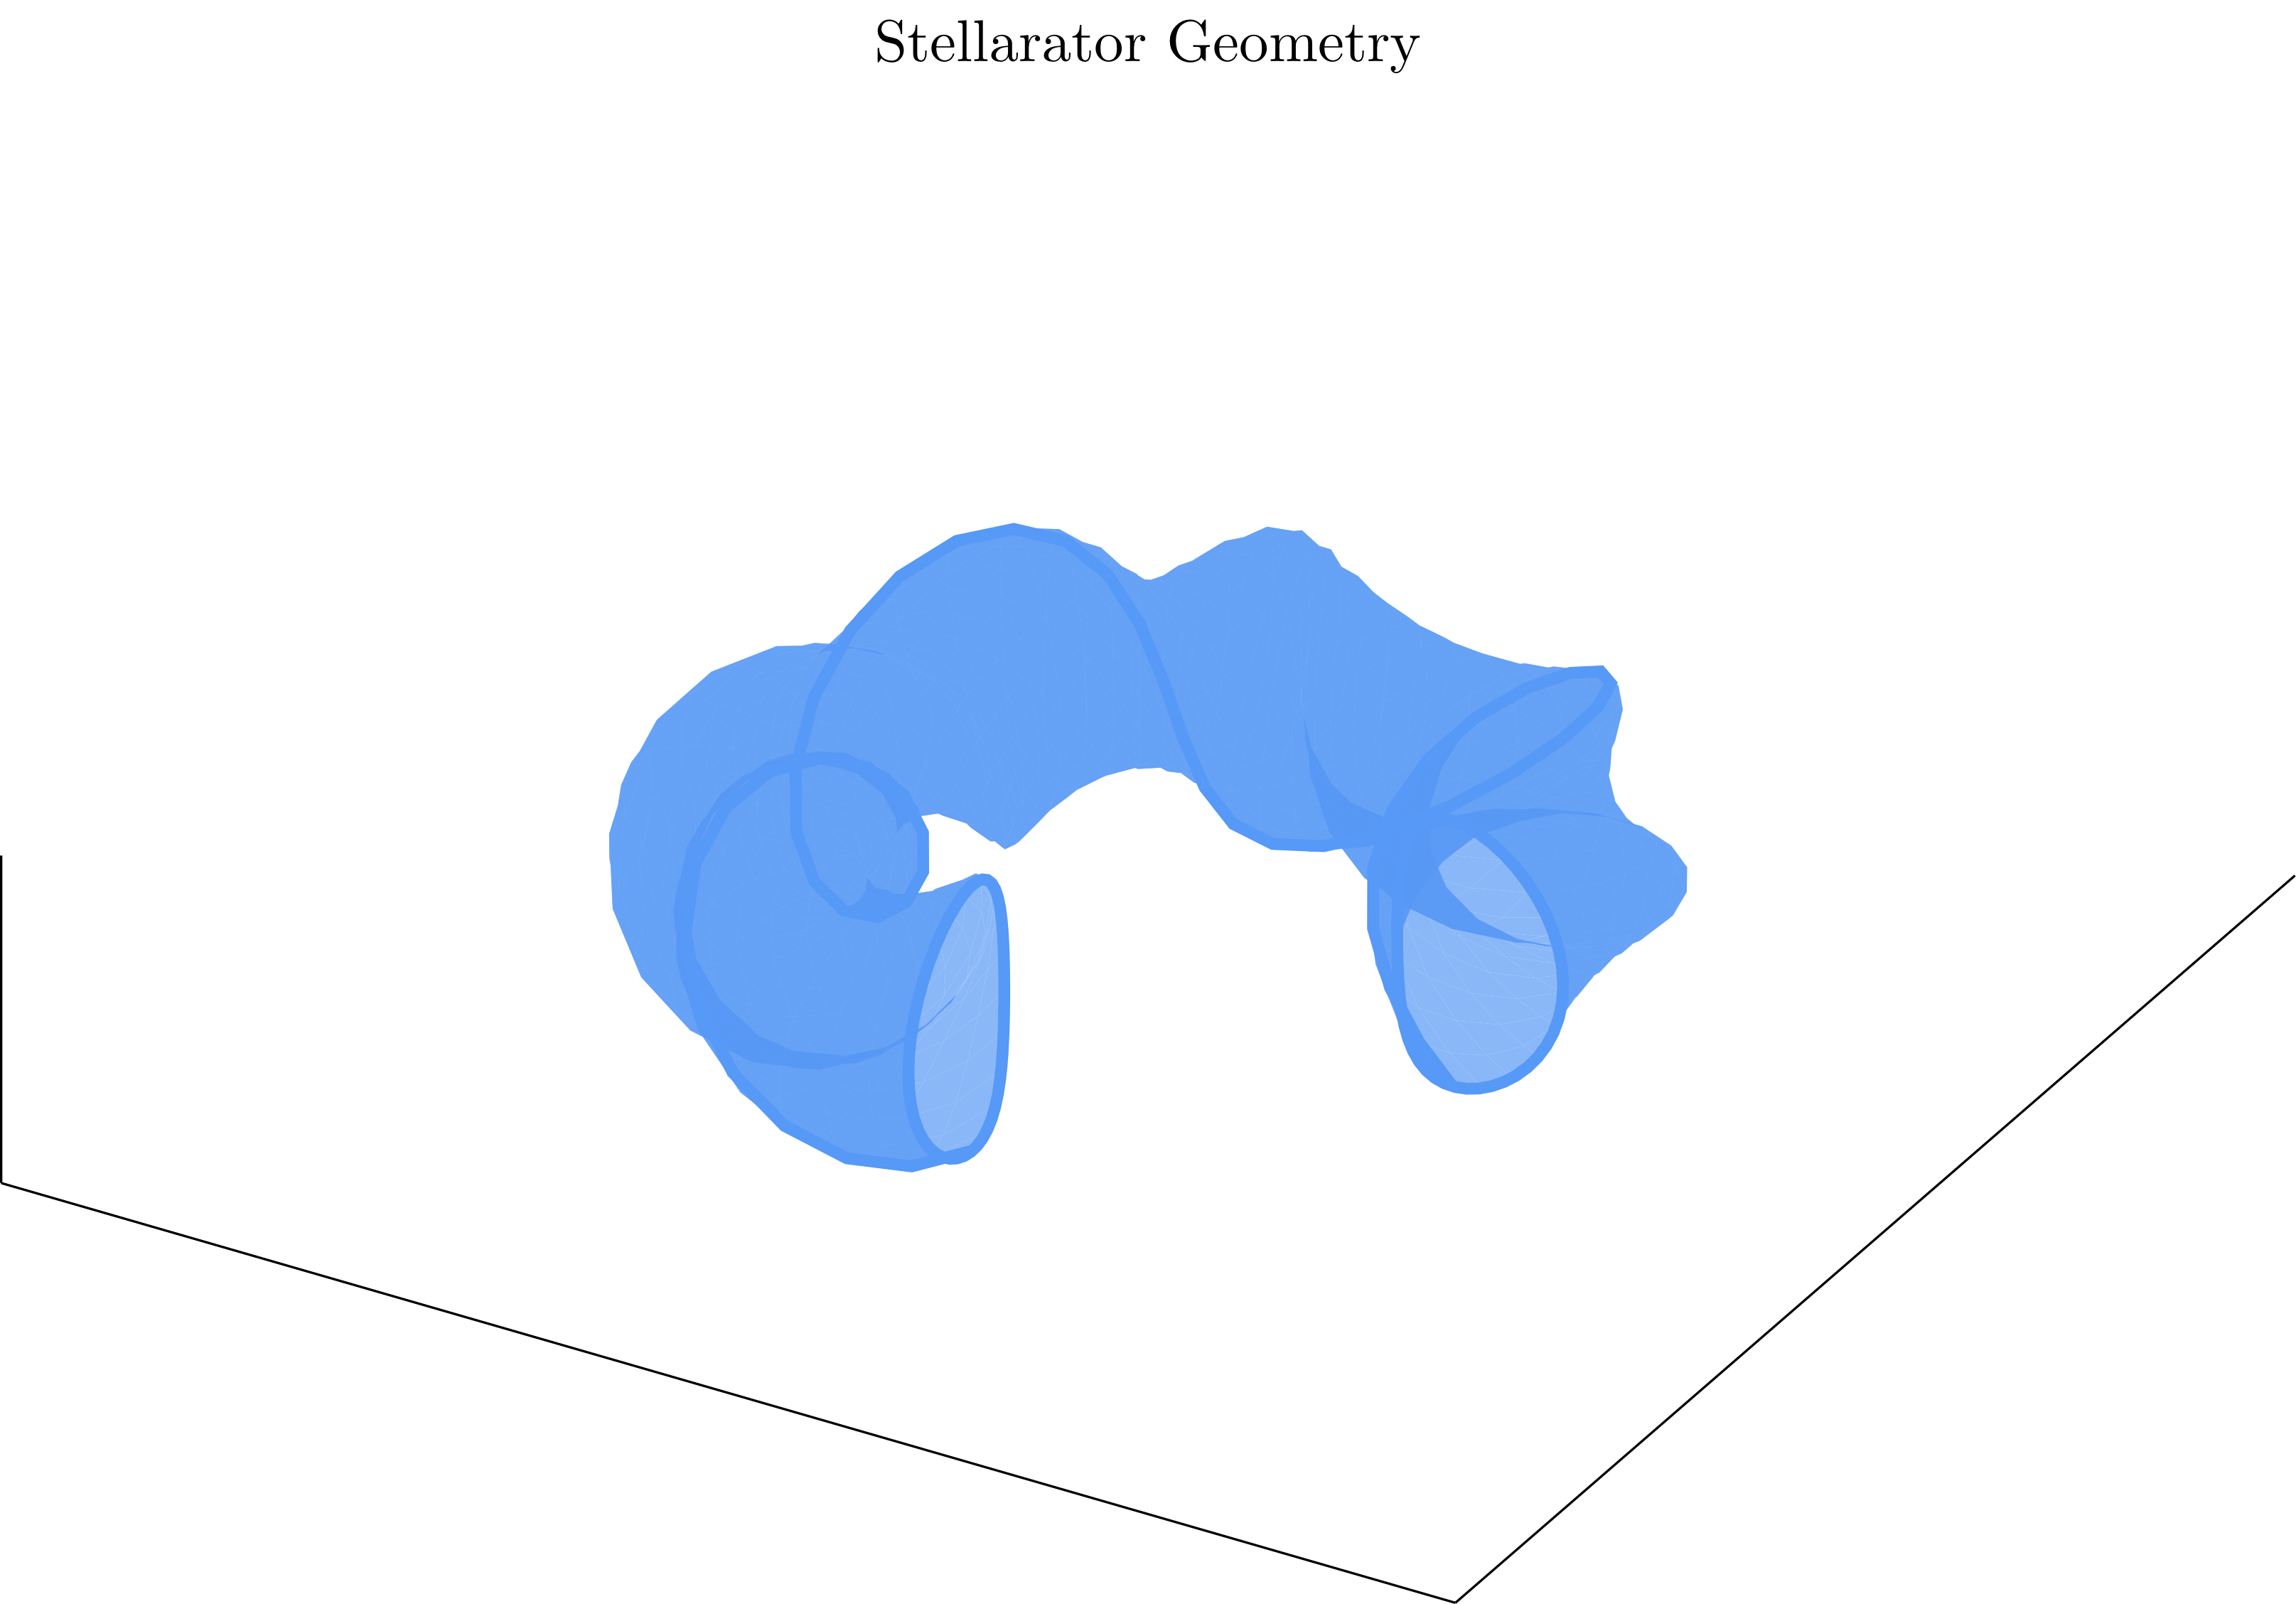
\includegraphics[width=0.725\textwidth]{images/stellarator}
	\caption{Cut-Away of Stellarator Reactor} ~\\
	\label{fig:stellar_cutaway} ~\\
	\small{A stellarator has a geometry similar to a tokamak, except it twists around its major axis. This eliminates the need for net current to keep the device in equilibrium.}
\end{figure}

\added{To model Ladon, this paper's proposed stellarator, one would need to replace at least: the Greenwald density limit and the confinement time scaling law. In place of the Greenwald density will likely be some other density or current limit, possibly the Bremsstrahlung density limit.\cite{stellar} This may require the density to be carried throughout analysis -- thus appearing explicitly in one column of \cref{table:eq}.}

\deleted{Optimistically, expanding this model would just involve developing a new confinement time scaling law and replacing the Greenwald density limit. The reason the Greenwald density limit is no longer important is because stability is much easier to maintain in a stellarator. Most likely, the density limit will now be governed by Bremsstrahlung radiation. If this were the case, each equation would need to be redivided using it. Ladon would be the reactor built using this enhancement.}

\section{Making a \replaced{Composite}{Hybrid} Reactor -- Janus}

The next interesting reactor would be a \replaced{composite}{hybrid} tokamak incorporating pulsed and steady-state operation: Janus. Fundamentally, this would involve current coming from both LHCD (steady-state), as well as inductive (pulsed) sources. How the two can coexist is shown in \cref{fig:cur_balance_final}. This was actually used in DEMO Pulsed, but the current drive was not handled self-consistently. Coupling these two current sources could reduce reliance on bootstrap current and lead to much more compact machines.

\begin{figure}
	\centering
	\begin{adjustbox}{width=0.75\textwidth}
		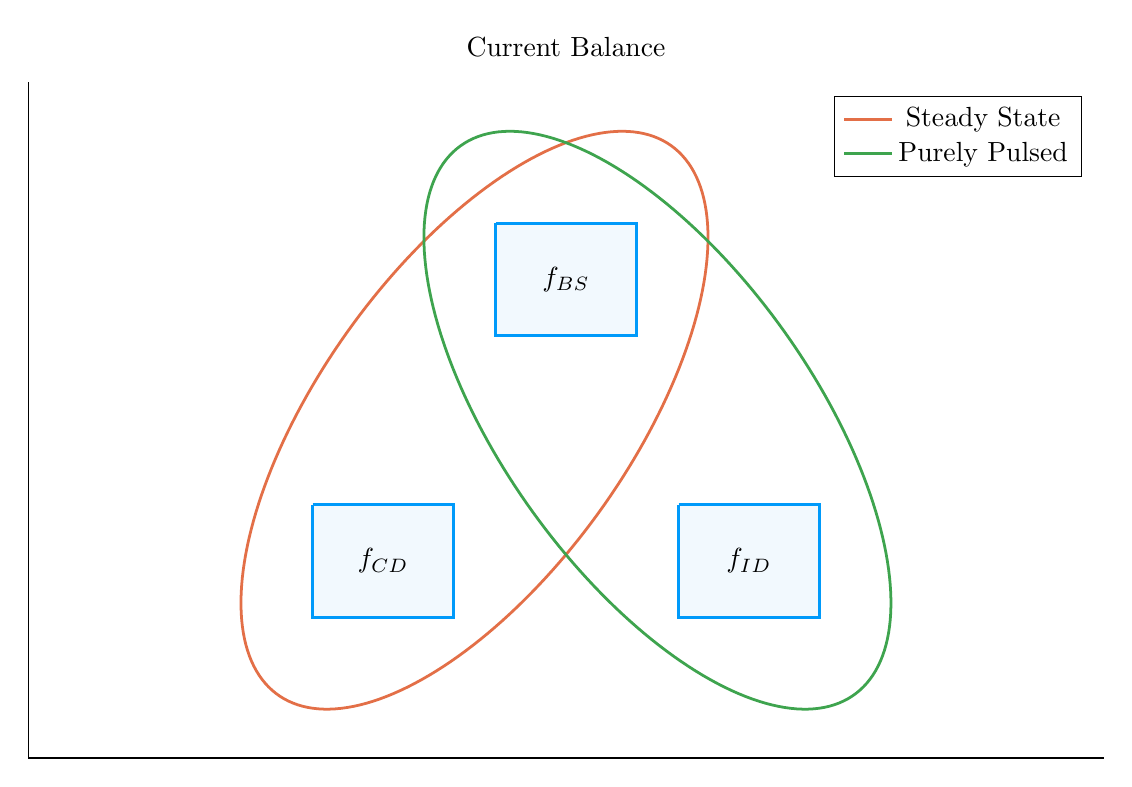
\begin{tikzpicture}[]
\begin{axis}[height = {101.6mm}, axis equal = {true}, ylabel = {}, title = {Current Balance}, xmin = {-5.773116112756781}, xmax = {5.773116112756781}, ymax = {6}, xlabel = {}, {unbounded coords=jump, scaled x ticks = false, xticklabel style={rotate = 0}, xmajorticks=false, xmajorgrids = false, axis lines* = left, scaled y ticks = false, yticklabel style={rotate = 0}, ymajorticks=false, ymajorgrids = false, axis lines* = left,     xshift = 0.0mm,
    yshift = 0.0mm,
    axis background/.style={fill={rgb,1:red,1.00000000;green,1.00000000;blue,1.00000000}}
}, ymin = {-6}, width = {152.4mm}]\addplot+ [color = {rgb,1:red,0.00000000;green,0.60560316;blue,0.97868012},
draw opacity=1.0,
line width=1,
solid,mark = none,
mark size = 2.0,
mark options = {
    color = {rgb,1:red,0.00000000;green,0.00000000;blue,0.00000000}, draw opacity = 1.0,
    fill = {rgb,1:red,0.00000000;green,0.60560316;blue,0.97868012}, fill opacity = 1.0,
    line width = 1,
    rotate = 0,
    solid
},fill = {rgb,1:red,0.00000000;green,0.60560316;blue,0.97868012}, fill opacity=0.05,forget plot]coordinates {
(-1.25, 3.5)
(1.25, 3.5)
(1.25, 1.5)
(-1.25, 1.5)
(-1.25, 3.5)
};
\addplot+ [color = {rgb,1:red,0.00000000;green,0.60560316;blue,0.97868012},
draw opacity=1.0,
line width=1,
solid,mark = none,
mark size = 2.0,
mark options = {
    color = {rgb,1:red,0.00000000;green,0.00000000;blue,0.00000000}, draw opacity = 1.0,
    fill = {rgb,1:red,0.00000000;green,0.60560316;blue,0.97868012}, fill opacity = 1.0,
    line width = 1,
    rotate = 0,
    solid
},fill = {rgb,1:red,0.00000000;green,0.60560316;blue,0.97868012}, fill opacity=0.05,forget plot]coordinates {
(-4.5, -1.5)
(-2.0, -1.5)
(-2.0, -3.5)
(-4.5, -3.5)
(-4.5, -1.5)
};
\addplot+ [color = {rgb,1:red,0.00000000;green,0.60560316;blue,0.97868012},
draw opacity=1.0,
line width=1,
solid,mark = none,
mark size = 2.0,
mark options = {
    color = {rgb,1:red,0.00000000;green,0.00000000;blue,0.00000000}, draw opacity = 1.0,
    fill = {rgb,1:red,0.00000000;green,0.60560316;blue,0.97868012}, fill opacity = 1.0,
    line width = 1,
    rotate = 0,
    solid
},fill = {rgb,1:red,0.00000000;green,0.60560316;blue,0.97868012}, fill opacity=0.05,forget plot]coordinates {
(2.0, -1.5)
(4.5, -1.5)
(4.5, -3.5)
(2.0, -3.5)
(2.0, -1.5)
};
\addplot+ [color = {rgb,1:red,0.88887350;green,0.43564919;blue,0.27812294},
draw opacity=1.0,
line width=1,
solid,mark = none,
mark size = 2.0,
mark options = {
    color = {rgb,1:red,0.00000000;green,0.00000000;blue,0.00000000}, draw opacity = 1.0,
    fill = {rgb,1:red,0.88887350;green,0.43564919;blue,0.27812294}, fill opacity = 1.0,
    line width = 1,
    rotate = 0,
    solid
}]coordinates {
(1.8698661812068136, 4.877080107549691)
(1.7975582266118808, 4.9252162522328415)
(1.7218385915440537, 4.9684428342438745)
(1.6427827549822935, 5.006716764385765)
(1.5604695215037632, 5.03999989037258)
(1.4749809427297138, 5.068259034860505)
(1.3864022355346433, 5.091466028519745)
(1.2948216971002622, 5.109597738114323)
(1.2003306168989445, 5.122636089561793)
(1.1030231856943935, 5.130568085949879)
(1.0029964016502424, 5.133385820492077)
(0.9003499736401737, 5.131086484409318)
(0.7951862218559462, 5.123672369729815)
(0.6876099758124048, 5.111150867004319)
(0.5777284698511354, 5.093534457939059)
(0.46565123624694493, 5.07084070295371)
(0.35148999602370634, 5.043092223676775)
(0.23535854758841435, 5.010316680395862)
(0.11737265329445545, 4.972546744485303)
(-0.00235007595282255, 4.929820065838624)
(-0.12369029793321751, 4.882179235338303)
(-0.2465270580745944, 4.829671742400261)
(-0.37073791002303214, 4.77234992763537)
(-0.49619903770001583, 4.710270930675205)
(-0.6227853787249911, 4.643496633214007)
(-0.7503707490802689, 4.572093597323671)
(-0.878827968893996, 4.496132999103221)
(-1.0080289892158198, 4.415690557728926)
(-1.137845019658864, 4.330846459975782)
(-1.26814665678079, 4.241685280285592)
(-1.3988040130759585, 4.148295896461316)
(-1.5296868464501256, 4.050771401071749)
(-1.6606646900485882, 3.949209008654826)
(-1.7916069823083864, 3.8437099588120507)
(-1.9223831971049103, 3.734379415290662)
(-2.0528629738631725, 3.6213263611541278)
(-2.1829162475040724, 3.5046634901454468)
(-2.3124133780960925, 3.3845070943515854)
(-2.4412252800831986, 3.26097694828099)
(-2.5692235509601344, 3.1341961894697543)
(-2.696280599266827, 3.004291195735447)
(-2.822269771774333, 2.8713914592009493)
(-2.947065479735527, 2.735629457213896)
(-3.0705433240746993, 2.597140520290374)
(-3.192580219391261, 2.4560626972145165)
(-3.3130545166539442, 2.3125366174284774)
(-3.4318461244632026, 2.166705350849943)
(-3.5488366287609345, 2.0187142652569277)
(-3.6639094108681878, 1.8687108813820061)
(-3.776949763733194, 1.7168447258604496)
(-3.8878450062738565, 1.5632671821788118)
(-3.9964845957006974, 1.4081313397725874)
(-4.1027602377083205, 1.2515918414233274)
(-4.206565994425528, 1.0938047291073505)
(-4.307798390016492, 0.9349272884497156)
(-4.4063565138277205, 0.7751178919384804)
(-4.502142120977991, 0.614535841055565)
(-4.595059730290983, 0.4533412074815748)
(-4.685016719472996, 0.29169467353285894)
(-4.771923417440856, 0.12975737198989234)
(-4.8556931937080146, -0.032309274523392384)
(-4.936242544739693, -0.1943437144491822)
(-5.013491177191022, -0.3561844283338884)
(-5.087362087945198, -0.5176700898342566)
(-5.157781640871865, -0.6786397265309694)
(-5.224679640229201, -0.8389328803894542)
(-5.287989400636577, -0.9983897677079463)
(-5.347647813547976, -1.1568514383933535)
(-5.403595410159981, -1.3141599344061687)
(-5.455776420691558, -1.4701584472164726)
(-5.504138829976595, -1.6246914741140965)
(-5.548634429313749, -1.7776049732170973)
(-5.589218864521925, -1.9287465170240605)
(-5.625851680153492, -2.0779654443571474)
(-5.658496359821148, -2.225113010544426)
(-5.687120362598258, -2.3700425356918093)
(-5.711695155456349, -2.5126095508967543)
(-5.732196241707455, -2.6526719422580065)
(-5.74860318542295, -2.7900900925378296)
(-5.760899631804527, -2.9247270203354994)
(-5.769073323487013, -3.0564485166333526)
(-5.773116112756781, -3.1851232785792454)
(-5.773023969673565, -3.3106230403720964)
(-5.768796986087595, -3.432822701120024)
(-5.760439375548035, -3.551600449543642)
(-5.747959469102832, -3.6668378854001826)
(-5.731369706994138, -3.778420137507439)
(-5.710686626257609, -3.8862359782498594)
(-5.685930844237935, -3.9901779344526522)
(-5.657127038037011, -4.090142394513381)
(-5.624303919915274, -4.186029711684261)
(-5.587494208670695, -4.2777443034022165)
(-5.546734597023965, -4.365194746567642)
(-5.502065715042401, -4.448293868676952)
(-5.453532089639006, -4.526958834718015)
(-5.4011821001870715, -4.601111229741906)
(-5.345067930294576, -4.67067713702862)
(-5.285245515786418, -4.735587211768881)
(-5.221774488946376, -4.795776750188546)
(-5.154718119074351, -4.851185754046737)
(-5.084143249418149, -4.901758990443393)
(-5.010120230542682, -4.947446046876624)
(-4.932722850202994, -4.98820138149499)
(-4.852028259791015, -5.023984368494613)
(-4.768116897429388, -5.054759338615853)
(-4.681072407788987, -5.080495614699213)
(-4.590981558710103, -5.101167542264987)
(-4.497934154710361, -5.116754515086211)
(-4.40202294746563, -5.127240995729401)
(-4.303343543353135, -5.132616531042591)
(-4.201994308148942, -5.132875762575277)
(-4.098076268974807, -5.1280184319198305)
(-3.9916930135921564, -5.118049380969083)
(-3.88295058714354, -5.102978547089826)
(-3.7719573864445346, -5.082820953217027)
(-3.658824051931438, -5.0575966928786364)
(-3.543663357372476, -5.02733091016593)
(-3.4265900974524626, -4.9920537746693245)
(-3.3077209733429527, -4.951800451404678)
(-3.1871744763719843, -4.906611065760036)
(-3.065070769909341, -4.8565306634977725)
(-2.941531569585093, -4.801609165851993)
(-2.816680021960811, -4.741901319765965)
(-2.690640581774395, -4.677466643319172)
(-2.5635388878808865, -4.608369366398399)
(-2.435501638012921, -4.5346783666719865)
(-2.306656462485676, -4.456467100931064)
(-2.1771317969721977, -4.373813531866238)
(-2.047056754475925, -4.286800050352669)
(-1.9165609966280504, -4.1955133933210735)
(-1.785774604437966, -4.100044557296444)
(-1.654827948625708, -4.00048870769076)
(-1.523851559665576, -3.896945083940012)
(-1.3929759976705065, -3.7895169005801836)
(-1.26233172224694, -3.678311244360763)
(-1.132048962449818, -3.5634389674983264)
(-1.0022575869674537, -3.4450145771766545)
(-0.8730869746655892, -3.323156121403477)
(-0.7446658856197179, -3.1979850713376368)
(-0.6171223327642645, -3.069626200204022)
(-0.49058345428648176, -2.938207458916877)
(-0.3651753868923626, -2.803859848535569)
(-0.24102314007082093, -2.666717289679875)
(-0.11825047148150092, -2.526916489034983)
(0.0030202364095237577, -2.384596803079324)
(0.12266809832327996, -2.2399000991709683)
(0.2405738466689491, -2.09297061413119)
(0.3566199504324037, -1.9439548104660527)
(0.4706907323336891, -1.7930012303693847)
(0.5826724841366269, -1.6402603476527216)
(0.6924535799956866, -1.4858844177497015)
(0.7999245877270309, -1.3300273259445707)
(0.9049783778929097, -1.1728444339759707)
(1.0075102305906167, -1.0144924251689658)
(1.1074179398395505, -0.8551291482497284)
(1.20460191546238, -0.6949134599984598)
(1.2989652823586764, -0.534005066897528)
(1.3904139770721349, -0.3725643659325606)
(1.478856841555075, -0.210752284705227)
(1.564205714036751, -0.04873012101713625)
(1.6463755169049392, 0.11334061791535466)
(1.725284341513138, 0.27529837645501054)
(1.8008535298288972, 0.4369817115859278)
(1.8730077528418523, 0.598229453843409)
(1.9416750856533156, 0.7588808679712085)
(2.0067870791725912, 0.9187758131459416)
(2.0682788283485025, 1.0777549026089095)
(2.126089036868173, 1.2356596625463219)
(2.1801600782585133, 1.3923326900594108)
(2.2304380533295443, 1.5476178100670777)
(2.2768728439022907, 1.7013602309846187)
(2.3194181627676604, 1.8534066990233193)
(2.358031599826549, 2.0036056509571933)
(2.392674664365143, 2.1518073652044736)
(2.423312823423304, 2.2978641110733555)
(2.4499155362177776, 2.4416302960231726)
(2.4724562845859026, 2.5829626107941834)
(2.490912599419497, 2.7217201722613846)
(2.505266083062553, 2.857764663869852)
(2.5155024276504205, 2.990960473511697)
(2.521611429372199, 3.12117482870718)
(2.5235869986421147, 3.2482779289551793)
(2.5214271661697554, 3.3721430751211794)
(2.515134084923101, 3.4926467957337035)
(2.5047140279823985, 3.609668970063368)
(2.4901773822870172, 3.7230929478618506)
(2.471538638281525, 3.8328056656413696)
(2.448816375471295, 3.9386977593788552)
(2.422033243902053, 4.040663673532358)
(2.391215941581816, 4.1386017662611385)
(2.356395187867742, 4.232414410744436)
(2.317605692844403, 4.322008092498024)
(2.274886122724018, 4.4072935025914814)
(2.2282790613031342, 4.488185626673267)
(2.1778309675141685, 4.564603829714885)
(2.123592129114139, 4.636471936389625)
(2.06561661255673, 4.70371830700579)
(2.0039622090976756, 4.766275908918702)
(1.9386903771871857, 4.824082383350291)
(1.869866181206814, 4.877080107549691)
};
\addlegendentry{Steady State}
\addplot+ [color = {rgb,1:red,0.24222430;green,0.64327509;blue,0.30444865},
draw opacity=1.0,
line width=1,
solid,mark = none,
mark size = 2.0,
mark options = {
    color = {rgb,1:red,0.00000000;green,0.00000000;blue,0.00000000}, draw opacity = 1.0,
    fill = {rgb,1:red,0.24222430;green,0.64327509;blue,0.30444865}, fill opacity = 1.0,
    line width = 1,
    rotate = 0,
    solid
}]coordinates {
(-1.8698661812068136, 4.877080107549691)
(-1.7975582266118808, 4.9252162522328415)
(-1.7218385915440537, 4.9684428342438745)
(-1.6427827549822935, 5.006716764385765)
(-1.5604695215037632, 5.03999989037258)
(-1.4749809427297138, 5.068259034860505)
(-1.3864022355346433, 5.091466028519745)
(-1.2948216971002622, 5.109597738114323)
(-1.2003306168989445, 5.122636089561793)
(-1.1030231856943935, 5.130568085949879)
(-1.0029964016502424, 5.133385820492077)
(-0.9003499736401737, 5.131086484409318)
(-0.7951862218559462, 5.123672369729815)
(-0.6876099758124048, 5.111150867004319)
(-0.5777284698511354, 5.093534457939059)
(-0.46565123624694493, 5.07084070295371)
(-0.35148999602370634, 5.043092223676775)
(-0.23535854758841435, 5.010316680395862)
(-0.11737265329445545, 4.972546744485303)
(0.00235007595282255, 4.929820065838624)
(0.12369029793321751, 4.882179235338303)
(0.2465270580745944, 4.829671742400261)
(0.37073791002303214, 4.77234992763537)
(0.49619903770001583, 4.710270930675205)
(0.6227853787249911, 4.643496633214007)
(0.7503707490802689, 4.572093597323671)
(0.878827968893996, 4.496132999103221)
(1.0080289892158198, 4.415690557728926)
(1.137845019658864, 4.330846459975782)
(1.26814665678079, 4.241685280285592)
(1.3988040130759585, 4.148295896461316)
(1.5296868464501256, 4.050771401071749)
(1.6606646900485882, 3.949209008654826)
(1.7916069823083864, 3.8437099588120507)
(1.9223831971049103, 3.734379415290662)
(2.0528629738631725, 3.6213263611541278)
(2.1829162475040724, 3.5046634901454468)
(2.3124133780960925, 3.3845070943515854)
(2.4412252800831986, 3.26097694828099)
(2.5692235509601344, 3.1341961894697543)
(2.696280599266827, 3.004291195735447)
(2.822269771774333, 2.8713914592009493)
(2.947065479735527, 2.735629457213896)
(3.0705433240746993, 2.597140520290374)
(3.192580219391261, 2.4560626972145165)
(3.3130545166539442, 2.3125366174284774)
(3.4318461244632026, 2.166705350849943)
(3.5488366287609345, 2.0187142652569277)
(3.6639094108681878, 1.8687108813820061)
(3.776949763733194, 1.7168447258604496)
(3.8878450062738565, 1.5632671821788118)
(3.9964845957006974, 1.4081313397725874)
(4.1027602377083205, 1.2515918414233274)
(4.206565994425528, 1.0938047291073505)
(4.307798390016492, 0.9349272884497156)
(4.4063565138277205, 0.7751178919384804)
(4.502142120977991, 0.614535841055565)
(4.595059730290983, 0.4533412074815748)
(4.685016719472996, 0.29169467353285894)
(4.771923417440856, 0.12975737198989234)
(4.8556931937080146, -0.032309274523392384)
(4.936242544739693, -0.1943437144491822)
(5.013491177191022, -0.3561844283338884)
(5.087362087945198, -0.5176700898342566)
(5.157781640871865, -0.6786397265309694)
(5.224679640229201, -0.8389328803894542)
(5.287989400636577, -0.9983897677079463)
(5.347647813547976, -1.1568514383933535)
(5.403595410159981, -1.3141599344061687)
(5.455776420691558, -1.4701584472164726)
(5.504138829976595, -1.6246914741140965)
(5.548634429313749, -1.7776049732170973)
(5.589218864521925, -1.9287465170240605)
(5.625851680153492, -2.0779654443571474)
(5.658496359821148, -2.225113010544426)
(5.687120362598258, -2.3700425356918093)
(5.711695155456349, -2.5126095508967543)
(5.732196241707455, -2.6526719422580065)
(5.74860318542295, -2.7900900925378296)
(5.760899631804527, -2.9247270203354994)
(5.769073323487013, -3.0564485166333526)
(5.773116112756781, -3.1851232785792454)
(5.773023969673565, -3.3106230403720964)
(5.768796986087595, -3.432822701120024)
(5.760439375548035, -3.551600449543642)
(5.747959469102832, -3.6668378854001826)
(5.731369706994138, -3.778420137507439)
(5.710686626257609, -3.8862359782498594)
(5.685930844237935, -3.9901779344526522)
(5.657127038037011, -4.090142394513381)
(5.624303919915274, -4.186029711684261)
(5.587494208670695, -4.2777443034022165)
(5.546734597023965, -4.365194746567642)
(5.502065715042401, -4.448293868676952)
(5.453532089639006, -4.526958834718015)
(5.4011821001870715, -4.601111229741906)
(5.345067930294576, -4.67067713702862)
(5.285245515786418, -4.735587211768881)
(5.221774488946376, -4.795776750188546)
(5.154718119074351, -4.851185754046737)
(5.084143249418149, -4.901758990443393)
(5.010120230542682, -4.947446046876624)
(4.932722850202994, -4.98820138149499)
(4.852028259791015, -5.023984368494613)
(4.768116897429388, -5.054759338615853)
(4.681072407788987, -5.080495614699213)
(4.590981558710103, -5.101167542264987)
(4.497934154710361, -5.116754515086211)
(4.40202294746563, -5.127240995729401)
(4.303343543353135, -5.132616531042591)
(4.201994308148942, -5.132875762575277)
(4.098076268974807, -5.1280184319198305)
(3.9916930135921564, -5.118049380969083)
(3.88295058714354, -5.102978547089826)
(3.7719573864445346, -5.082820953217027)
(3.658824051931438, -5.0575966928786364)
(3.543663357372476, -5.02733091016593)
(3.4265900974524626, -4.9920537746693245)
(3.3077209733429527, -4.951800451404678)
(3.1871744763719843, -4.906611065760036)
(3.065070769909341, -4.8565306634977725)
(2.941531569585093, -4.801609165851993)
(2.816680021960811, -4.741901319765965)
(2.690640581774395, -4.677466643319172)
(2.5635388878808865, -4.608369366398399)
(2.435501638012921, -4.5346783666719865)
(2.306656462485676, -4.456467100931064)
(2.1771317969721977, -4.373813531866238)
(2.047056754475925, -4.286800050352669)
(1.9165609966280504, -4.1955133933210735)
(1.785774604437966, -4.100044557296444)
(1.654827948625708, -4.00048870769076)
(1.523851559665576, -3.896945083940012)
(1.3929759976705065, -3.7895169005801836)
(1.26233172224694, -3.678311244360763)
(1.132048962449818, -3.5634389674983264)
(1.0022575869674537, -3.4450145771766545)
(0.8730869746655892, -3.323156121403477)
(0.7446658856197179, -3.1979850713376368)
(0.6171223327642645, -3.069626200204022)
(0.49058345428648176, -2.938207458916877)
(0.3651753868923626, -2.803859848535569)
(0.24102314007082093, -2.666717289679875)
(0.11825047148150092, -2.526916489034983)
(-0.0030202364095237577, -2.384596803079324)
(-0.12266809832327996, -2.2399000991709683)
(-0.2405738466689491, -2.09297061413119)
(-0.3566199504324037, -1.9439548104660527)
(-0.4706907323336891, -1.7930012303693847)
(-0.5826724841366269, -1.6402603476527216)
(-0.6924535799956866, -1.4858844177497015)
(-0.7999245877270309, -1.3300273259445707)
(-0.9049783778929097, -1.1728444339759707)
(-1.0075102305906167, -1.0144924251689658)
(-1.1074179398395505, -0.8551291482497284)
(-1.20460191546238, -0.6949134599984598)
(-1.2989652823586764, -0.534005066897528)
(-1.3904139770721349, -0.3725643659325606)
(-1.478856841555075, -0.210752284705227)
(-1.564205714036751, -0.04873012101713625)
(-1.6463755169049392, 0.11334061791535466)
(-1.725284341513138, 0.27529837645501054)
(-1.8008535298288972, 0.4369817115859278)
(-1.8730077528418523, 0.598229453843409)
(-1.9416750856533156, 0.7588808679712085)
(-2.0067870791725912, 0.9187758131459416)
(-2.0682788283485025, 1.0777549026089095)
(-2.126089036868173, 1.2356596625463219)
(-2.1801600782585133, 1.3923326900594108)
(-2.2304380533295443, 1.5476178100670777)
(-2.2768728439022907, 1.7013602309846187)
(-2.3194181627676604, 1.8534066990233193)
(-2.358031599826549, 2.0036056509571933)
(-2.392674664365143, 2.1518073652044736)
(-2.423312823423304, 2.2978641110733555)
(-2.4499155362177776, 2.4416302960231726)
(-2.4724562845859026, 2.5829626107941834)
(-2.490912599419497, 2.7217201722613846)
(-2.505266083062553, 2.857764663869852)
(-2.5155024276504205, 2.990960473511697)
(-2.521611429372199, 3.12117482870718)
(-2.5235869986421147, 3.2482779289551793)
(-2.5214271661697554, 3.3721430751211794)
(-2.515134084923101, 3.4926467957337035)
(-2.5047140279823985, 3.609668970063368)
(-2.4901773822870172, 3.7230929478618506)
(-2.471538638281525, 3.8328056656413696)
(-2.448816375471295, 3.9386977593788552)
(-2.422033243902053, 4.040663673532358)
(-2.391215941581816, 4.1386017662611385)
(-2.356395187867742, 4.232414410744436)
(-2.317605692844403, 4.322008092498024)
(-2.274886122724018, 4.4072935025914814)
(-2.2282790613031342, 4.488185626673267)
(-2.1778309675141685, 4.564603829714885)
(-2.123592129114139, 4.636471936389625)
(-2.06561661255673, 4.70371830700579)
(-2.0039622090976756, 4.766275908918702)
(-1.9386903771871857, 4.824082383350291)
(-1.869866181206814, 4.877080107549691)
};
\addlegendentry{Purely Pulsed}
\node at (axis cs:0, 2.5) [,
color={rgb,1:red,0.00000000;green,0.00000000;blue,0.00000000}, draw opacity=1.0,
rotate=0.0
] {$f_{BS}$};
\node at (axis cs:-3.25, -2.5) [,
color={rgb,1:red,0.00000000;green,0.00000000;blue,0.00000000}, draw opacity=1.0,
rotate=0.0
] {$f_{CD}$};
\node at (axis cs:3.25, -2.5) [,
color={rgb,1:red,0.00000000;green,0.00000000;blue,0.00000000}, draw opacity=1.0,
rotate=0.0
] {$f_{ID}$};
\end{axis}

\end{tikzpicture}

	\end{adjustbox}
%	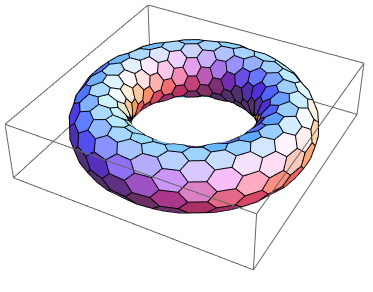
\includegraphics[width=0.75\textwidth]{images/test_image}
	\caption{Current Balance in a Tokamak} ~\\
	\small In a tokamak, there needs to be a certain amount of current -- and that current has to come from somewhere. All good reactors have an adequate bootstrap current. What provides the remaining current is what distinguishes steady state from pulsed operation.
	\label{fig:cur_balance_final}
\end{figure}

The arguments against this are mainly technical: why build two difficult auxiliary systems when one is needed -- especially when they probably work against each other. Although rational, \replaced{it may turn out that the larger current achievable with two sources leads to a smaller, more economic machine.}{the argument implicitly assumes a current is achievable through only one source (i.e.\ either through LHCD or from a central solenoid). Using two may allow for stronger plasma currents.}

\section{Bridging Confinement Scalings -- Daedalus}

The final potential reactor -- Daedalus -- is designed \replaced{so that it can be}{to collect as many scaling laws as possible. As a baseline, it should be able to} run in H-Mode, L-Mode, and I-Mode. Up until now, only H-Mode (high confinement) has been discussed due to its use in conventional reactor design. However, L-Mode (low) and I-Mode\cite{imode} (intermediate) may prove to produce more favorable scalings -- in terms of cost -- as more of reactor space is explored.

Because L-Mode is available on any machine, the first step is \added{actually} building under H-Mode. The goal then is to find reactors that can also reach I-Mode -- \replaced{simultaneously}{thus} improving the scaling law's fit and \added{possibly} making the actual reactor more \replaced{economic}{cost effective}.

Presented below are the three confinement scaling laws, as well as the generalized formula. As should be noted, the I-Mode scaling currently lacks a true radial dependence -- as it has only been found on two machines.\cite{imode} This is one reason Daedalus would be so valuable.\footnote{ In H-Mode and L-Mode's favor, they have been found on every machine that should see them. }

\begin{equation}
  \tau_E = K_\tau \, H \, \frac{
    I_P^{\,\alpha_I} \, R_0^{\,\alpha_R} \, a^{\,\alpha_a} \, \kappa^{\,\alpha_\kappa} \ \overline{n}^{\,\alpha_n} \, B_0^{\,\alpha_B} \, A^{\,\alpha_A}
  }{ P_{src} ^ {\,\alpha_P} }
  \tag{\ref{eq:tau_gen}}
\end{equation}

\begin{equation}
  \tau_E^H = 0.145 \, H \, \frac{
    I_P^{0.93} \, R_0^{1.39} \, a^{0.58} \, \kappa^{0.78} \ \overline{n}^{\, 0.41} \, B_0^{0.15} \, A^{0.19}
  }{ P_{src} ^ {\,0.69} }
  \tag{\ref{eq:tau_h}}
\end{equation}
\begin{equation}
  \tau_E^L = 0.048\, H \, \frac{
    I_P^{0.85} \, R_0^{1.2} \, a^{0.3} \, \kappa^{0.5} \ \overline{n}^{\, 0.1} \, B_0^{0.2} \, A^{0.5} }{ P_{src} ^ {\,0.5} }
\end{equation}
\myequations{ L-Mode Confinement Time Scaling Law -- $\tau_E^L$ }
\begin{equation}
  \tau_E^I = \frac{ 0.014 \, H }{ 0.68 ^ {\lambda_R} \cdot 0.22 ^ {\lambda_a} } \cdot \frac{ I_P^{0.69} \, R_0^{\lambda_R} \, a^{\lambda_a} \, \kappa^{0.0} \ \overline{n}^{\, 0.17} \, B_0^{0.77} \, A^{0.0} }{ P_{src} ^ {\,0.29} }
\end{equation}
\myequations{ I-Mode Confinement Time Scaling Law -- $\tau_E^I$ }
\begin{equation}
	\lambda_R + \lambda_a = 2.2
\end{equation}

A final point to make is reemphasizing that the I-Mode scaling law -- developed by the authors -- is \replaced{significantly underdeveloped.}{not battle-tested.} It is the target of ongoing research at the MIT PSFC.\cite{imode}

\section{Addressing Model Shortcomings}

Before moving on to the final conclusions, we will give a quick recap of \replaced{several of the more overly simplified phenomena in}{the more audacious simplifications used within} this fusion systems framework. These include: approximating temperature profiles as simple parabolas, neglecting all radiation except Bremsstrahlung, and handling flux sources at too basic a level. \added{This list is non-comprehensive, as more sophisticated analysis would also help: the divertor heat load, the neutron wall loading, etc.}

\subsection{Integrating Pedestal Temperature Profiles}

\replaced{One of the biggest shortcomings of this model is not handling plasma profiles self-consistently -- instead replacing them with simple parabolas.}{The most dubious simplification in the code at this point is modeling temperature profiles as parabolas.} Although these parabolas work for densities and L-Mode plasma temperatures, the same cannot be said about H-Mode temperatures. This is because they have a distinct pedestal region on the outer edge of the plasma.

The usage of pedestal temperatures -- discussed in \cref{chapter:profiles} -- improves two aspects of the model: the fusion power and the bootstrap current. These were shown in the results to be over-calculated and underestimated, respectively. Pedestals, having a lower core temperature, would decrease the total fusion power. As well, they would boost bootstrap current due to the quick drop near the plasma's edge (i.e.\ they have a large derivative there).

These improvements could easily be added to the code, because temperature was addressed as a difficult parameter to handle from the beginning.

\subsection{Expanding the Radiation Loss Term}

The next area that would be improved by more sophisticated theory would be the radiation loss term. From before, it was pointed out that the Bremsstrahlung radiation was the dominant term within the plasma core and, therefore, provided a first-order approximation. Drawing the radiation losses closer to real world values would involve adding line radiation and synchrotron radiation. The former of which would be needed as high-Z impurities become more important.

\subsection{Taking Flux Sources Seriously}

The final oversimplification in the model deals with the flux sources involved in a pulsed reactor -- existing at multiple level. First, the derivation of flux balance started with a simple transformer between a solenoid primary and a plasma secondary. \deleted{Even this initial step is probably too simple.}

After we developed an equation for flux balance, we compared it to ones in the literature (i.e.\ PROCESS) to build confidence in the model. To draw this equation closer to theirs, we then added a PF coil contribution a posteriori. This implicitly ignored coupling between most of the components. Thus leading to another source of error for the model. Moreover, this formula for PF coil contribution was much simpler than ones found in other fusion systems codes.

Even though this model may be extremely simple, it does remarkably well at matching more sophisticated codes -- and does so at a much faster pace. These suggestions were \deleted{all} just ways to \replaced{account for more realistic physics.}{draw results closer to real world values.}

%\end{document}

\chapter{Concluding Reactor Discussion}

\replaced{The goal of this document was to fairly compare pulsed and steady-state tokamaks -- using a single, comprehensive model. The main conclusion is that both modes of operation can produce economically competitive reactors, assuming some technological advancement. The advancement most supported by the results was in magnet technology, as MIT is currently exploring with high-temperature superconducting (HTS) tape.}{The goal of this document was to develop a simple fusion systems model that can work for both pulsed and steady-state tokamaks. The main conclusion was that the best way to build a more efficient, compact reactor is to invest in strong magnets -- as MIT is doing with high-temperature superconducting (HTS) tape. Further it was shown that to best utilize materials, the tape should be incorporated into the toroidal field coils for steady-state machines and in the central solenoid for pulsed ones.} \added{However a more fundamental result is that pulsed operation can be economically competitive and the United States should be putting a larger research effort behind it.}

\replaced{Although some skepticism should be allotted to these conclusions, it was shown that this simple algebraic solver was capable of matching more sophisticated frameworks with speed and ease. This model may not provide an engineer's level of rigor for cost measurements, but does produce empirically-drawn costing trends applicable to the target physics audience. Ultimately, it serves to complement higher dimension codes when researchers want to investigate new areas of reactor space.}{Although some skepticism should be allotted to these conclusions, it was shown that this simple algebraic solver matched sophisticated multiyear research studies with speed and ease. This model may not provide an engineer's rigor in measuring cost, but the same can be said for any code or theory. The fusion system is as nonlinear a problem as they come, but we still managed to build a framework that can hone even a well-trained physicist's intuition.}

\deleted{The final point to make is that this model actually predicts that HTS technology can provide the optimum magnetic field strength for a reactor. Once HTS doubles the maximum achievable teslas, the law of diminishing returns heavily kicks in. This of course assumes H-Mode D-T plasmas at the Greenwald density limit.}


\added{What the results truly show, though, is that no economic reactor can be built using existing technology -- regardless of whether it runs as pulsed or steady-state. This is why every design from the literature exceeds standard values for $H$ and $N_G$. Therefore, some technological advancement is needed. These may come from research and development into:}
\begin{itemize}[noitemsep,topsep=0pt]
	\item \added{building stronger magnets using HTS tape}
	\item \added{discovering reliable regimes of enhanced confinement}
	\item \added{producing higher bootstrap fractions with tailored profiles}
	\item \added{optimizing aspect ratio and elongation geometric parameters}
\end{itemize}

\added{As mentioned, using HTS tape to nearly double achievable magnet strengths is one such advancement capable of making reactors economically viable. To best utilize this resource, though, HTS tape should appear only in the TF coils for steady-state machines and in the central solenoid for pulsed ones. This was because the optimum toroidal field strength for pulsed machines was found to be achievable with conventional low-temperature superconducting (LTS) magnets.}

\added{Further, it was shown that past the regime of magnet strengths relevant to HTS, cost curves undergo considerably diminished returns. As such, HTS technology might be the final major magnet advancement in the current H-Mode, D-T plasma paradigm.}


\appendix

\chapter{Simulating with Fussy.jl}

Fussy.jl is a \underline{fus}ion \underline{sy}stems code written using the Julia language. The reason for choosing Julia over say Matlab and Python was due to metaprogramming concerns and its tight-knit  computational community, respectively. Incorporating the model used throughout this paper, the code is quick to run and matches more sophisticated frameworks with high fidelity.

This chapter will be broken down into three steps. The first is getting a user up and running with the code. Once the user gets to this point, hopefully they will wonder how the code is structured. This will be the second step. The final step will be explaining the various functions callable on reactor objects -- the atomic data structure for Fussy.jl.

\section{Getting the Code to Work}

The hardest step of any codebase is getting it up and running. These instructions should get a user to a point where they are a few internet searches away from a working copy of Fussy.jl. As an aide, you can view an interactive collection of Fussy.jl Jupyter notebooks at the following website:

{\centering \href{http://fusion.codes}{www.fusion.codes} \par }

Although \href{http://fusion.codes}{fusion.codes} is a nice tool for viewing this document's results, it is a little slow for producing new data -- and it also lacks a method for storing it. Therefore, an advanced user should first download a copy of Julia from:

{\centering \href{https://julialang.org/downloads}{julialang.org/downloads} \par }

Currently the Fussy.jl codebase is written using \texttt{v0.6}, but should be \texttt{v1.0} compatible by 2019. Using Julia nomenclature, Fussy.jl is a Julia package. It can be cloned using Julia conventions from the following Github repository:

{\centering \href{https://github.com/djsegal/Fussy.jl.git}{https://github.com/djsegal/Fussy.jl.git} \par }

Once the Fussy.jl package has been cloned into your Julia package library, you should be able to access it through the Julia REPL or a Jupyter notebook. You can now reproduce every plot in this text. A quick test to see if your code works is: \\

\texttt{using Fussy \\
cur\_reactor = Reactor(10) \\ \\
@assert cur\_reactor.T\_bar == 10
}

\section{Sorting out the Codebase}

Assuming the user got to this section, the code works and now you want to know what you can do with it. The place to start is in the \texttt{src} folder, again viewable online at:

{\centering \href{http://git.io/tokamak}{git.io/tokamak} \par }

Within the \texttt{src} folder are several subfolders as well as a few files (e.g. Fussy.jl and defaults.jl). In an attempt to not bore the reader, we will be painting with thick brushstrokes. Further, the \texttt{methods} subfolder will be the topic of the next section -- as most involve calls on a reactor object.

\subsection{Typing out Structures}

The place to start in any modeling framework is its data structures. These type definitions allow the building of nested hierarchies of constructed objects. The most atomic of these is the Reactor struct, but several other ones allow for solving broader scoped questions (i.e. Scans, Sensitivities, and Samplings.)

\subsubsection{The Reactor Structure}

Reactors are the most atomic data structure in this fusion systems model. They store all the fields needed to represent a reactor as it exists in reactor space. This obviously includes its temperature, current, and radius, but also includes derived quantities, such as the cost-per-watt and bootstrap fraction. They can be initialized, solved, updated, and honed. Most other data structures are just wrappers to hold these reactors -- they are described next.

\subsubsection{The Scan Structure}

A Scan object is a collection of reactors made from scanning a list of temperatures. For example, a scan of five temperatures from 5 keV to 25 keV would result in several arrays of five reactors. Most often, one of these lists would correspond to beta reactors, one to kink reactors, and one to wall loading reactors. There may then be fewer than five reactors in a list if some of the reactors are invalid or frankly unsolvable.

This is the data structure that produces the various comparison plots in the results section.

\subsubsection{The Sensitivity Structure}

Sensitivity studies are how computationalists test the effect of changing a variable over multiple values -- i.e. do a 20\% sensitivity around the H factor. Like Scans, Sensitivities store various lists of reactors, each corresponding to an interesting data point. These include limit reactors where the beta limit and kink limit are just satisfied or the beta limit and wall loading are just satisfied. Additionally, they include the minimum capital cost reactors and the minimum cost-per-watt ones. 

\subsubsection{The Sampling Structure}

The Sampling struct was created to do simple Monte Carlo runs over a reactor's fixed values. While sensitivities only allow one variable to change at a time, samplings randomly assign a list of variables to some neighborhood of possible values. These are how the colorful scatter plots are made. Succinctly, where sensitivity studies show local changes to variables, Monte Carlo samplings show global trends in reactor design.

\subsubsection{The Equation Structure}

In order to store the various equations from \cref{table:eq} is the Equation Struct. It stores the $\gamma$ exponents for: $R_0$, $B_0$, and $I_P$. It also stores the function representing G($\overline T$). Repeated these are the unknowns in:

\begin{equation}
	\tag{\ref{eq:rbi}}
	R_0^{\, \gamma_R} \cdot B_0^{\, \gamma_B} \cdot I_P^{\, \gamma_I} = G( \overline T )
\end{equation}

Concretely, there are 16 objects that use this struct -- one for each equation (e.g. for fusion power, the beta limit, and temperature assignment).

\subsubsection{The Equation Set Structure}

The step up from the Equation struct are the Equation Sets. These collections of three equations allow $R_0$, $B_0$, and maybe $I_P$ to be substituted out of the current balance root-solving equation. This is where \cref{eq:case_1_R,eq:case_1_B,eq:case_1_I,eq:case_1_gamma,eq:case_2_R,eq:case_2_B,eq:case_2_gamma} come into play.

\subsection{Referencing Input Decks and Solutions}

With more than twenty fixed variables in the model, the range of tokamak reactors is basically infinite. To help users build a net of designs to explore reactor space are seven input decks. These are the ones given in the results: Arc, Act I/II, Demo Steady/Pulsed, Proteus and Charybdis. Coupled with the non-prototype reactors are solution reactors that store various quantities from the original paper (e.g. $P_F$, $f_{BS}$, $R_0$). These are how the comparison tables were constructed.

\subsection{Acknowledging Utility Functions}

For the uninitiated, utility functions are grab bag functions that do not really belong in a codebase -- but do anyway. This sentiment does not mean they are worthless, just not fusion related at all. In Fussy.jl, the most notable are a normalized integral calculator, a filter that includes numeric tolerances, and a robust root solver. 

Although since incorporated into the official Roots.jl package, \texttt{find\_roots} allows finding an arbitrary number of roots within a bounded range. This was needed because many roots can be found at various levels of the reactor solving problem -- i.e. for $I_P$, $\overline T$, $\eta_{CD}$, etc.

\subsection{Mentioning Base Level Files}

In addition to subdirectories within the \texttt{src} folder are three files: Fussy.jl, abstracts.jl, and defaults.jl. Fussy.jl is the package's main file that actually stores the Fussy module. While, abstracts.jl stores various abstract structures that help clean up other files.

Finally, defaults.jl stores various default values that are important to the codebase. For example, this is where the various scaling law exponents are stored. It is also where the bounding values for the different root solving problems live. These include minimum and maximum values for: $I_P$, $\overline T$, $\eta_{CD}$.

Now that a majority of the files have been discussed, we can turn to the reactor methods. These constitute most of the interesting functionality within the codebase. 

\section{Delving into Reactor Methods}

The reactor is the most atomic data structure in this model. It therefore makes sense that it has many instance methods. These include all the coefficients, fluxes, powers, etc. It also includes methods that solve a reactor, perform a match on some field's value, or convert $\eta_{CD}$ to self-consistency. The various subdirectories within the \texttt{src/methods/reactors} folder will now be discussed.

\subsubsection{Calculations}

The calculation subdirectory of reactor methods are used to set various important values in the solver. For floating variables, these include: $\overline n$, $R_0$, $B_0$, and $I_P$. This folder also includes the calculation of the Bosch-Hale reactivity and the Ehst-Karney current drive efficiency. 

\subsubsection{Coefficients and Composites}

The coefficients and composites directories correspond to the model's fixed and floating coefficients, respectively. For clarity, fixed coefficients, including $K_n$ and $K_{CD}$, were labeled with a K. Whereas, floating coefficients then started with G's -- i.e. $G_{PB}$ and $G_V$.

\subsubsection{Fluxes and Powers}

Within flux balance and power balance were around a dozen terms or sub-terms. Although not directly used in the conservation equations, sub-terms are used to compare the model to ones from the literature. For clarity, fluxes include: $\Phi_{CS}$, $\Phi_{PF}$, $\Phi_{RU}$, $\Phi_{FT}$, $\Phi_{res}$, and $\Phi_{ind}$. The powers, then, include: $P_F$, $P_{BR}$, $P_\kappa$, $P_L$, $P_W$, etc. 

\subsubsection{Profiles}

The next collection of reactor methods are the various profiles. Most obviously, these include radial plasma profiles for density, temperature, and current. However, this folder also includes the magnetic field strength as a function of radius -- as was used within current drive efficiency calculations.

\subsubsection{Geometries}

Additionally, there are many geometric relations. These include the various tokamak thicknesses: a, b, c, d -- as well as the radius and height of the central solenoid. This group also includes the volume, perimeter, surface area, and cross-sectional area. As well as the many subscripted fields. For example, the elongation (i.e. $\kappa_{95}$) includes the following alternative definitions: $\kappa_X$, $\kappa_P$, and $\kappa_\tau$

\subsubsection{Formulas}

The final set of reactor methods are formulas that do not really fit anywhere else. If a method is not related to geometry, power, calculations, etc, it ends up here. For example, this group includes: $\beta_N$, $f_{BS}$, $C_W$, and $\tau_E$. Total, there are around 25 formulas.

At this point, you should now be an expert Fussy.jl user. Good luck!
\chapter{Selecting Plasma Profiles}

\label{chapter:profiles}

\begin{figure*}[h]
    \centering
    \hfill 
    \begin{subfigure}[t]{0.45\textwidth}
        \centering
		\begin{adjustbox}{width=\textwidth}
			\Large
			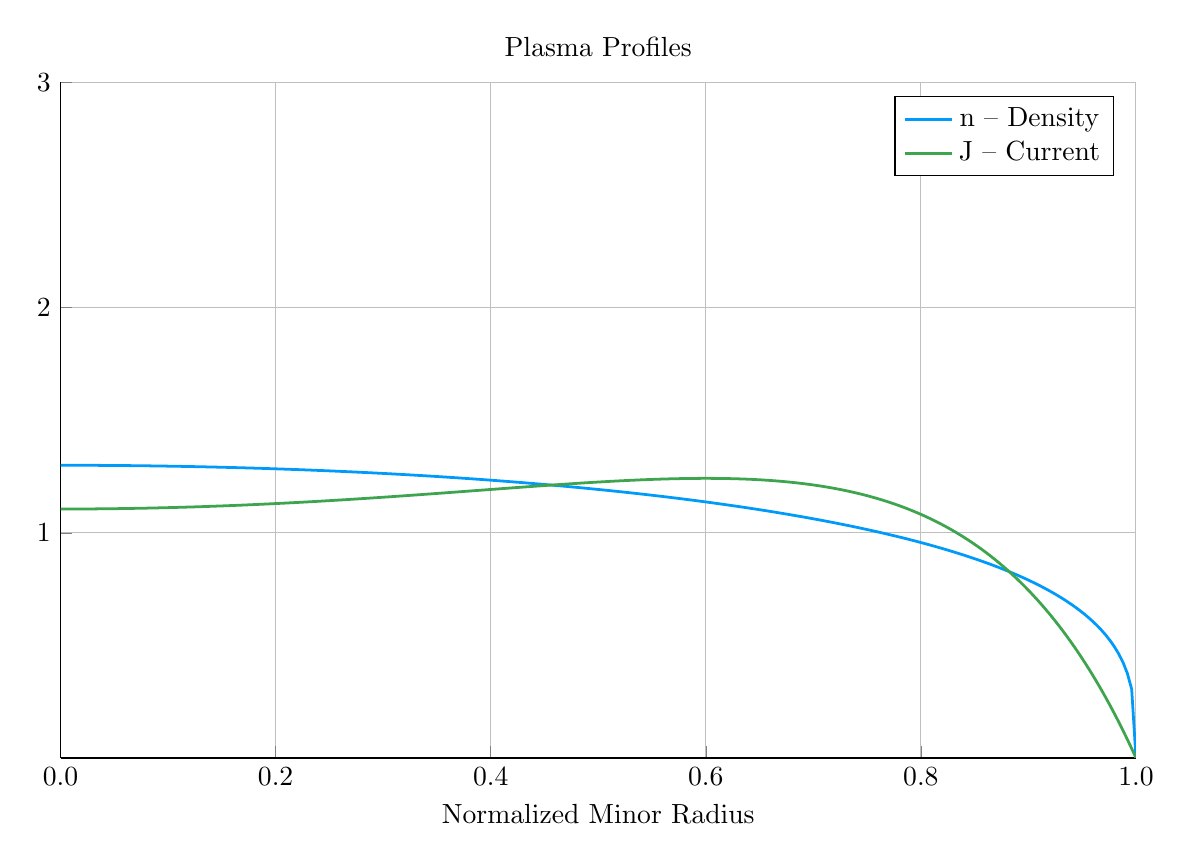
\begin{tikzpicture}[]
\begin{axis}[height = {101.6mm}, ylabel = {}, title = {Plasma Profiles}, xmin = {0.0}, xmax = {1.0}, ymax = {3}, xlabel = {Normalized Minor Radius}, {unbounded coords=jump, scaled x ticks = false, xticklabel style={rotate = 0}, xmajorgrids = true, xtick = {0.0,0.2,0.4,0.6000000000000001,0.8,1.0}, xticklabels = {0.0,0.2,0.4,0.6,0.8,1.0}, xtick align = inside, axis lines* = left, scaled y ticks = false, yticklabel style={rotate = 0}, ymajorgrids = true, ytick = {1.0,2.0,3.0}, yticklabels = {1,2,3}, ytick align = inside, axis lines* = left,     xshift = 0.0mm,
    yshift = 0.0mm,
    axis background/.style={fill={rgb,1:red,1.00000000;green,1.00000000;blue,1.00000000}}
}, ymin = {0}, width = {152.4mm}]\addplot+ [color = {rgb,1:red,0.00000000;green,0.60560316;blue,0.97868012},
draw opacity=1.0,
line width=1,
solid,mark = none,
mark size = 2.0,
mark options = {
    color = {rgb,1:red,0.00000000;green,0.00000000;blue,0.00000000}, draw opacity = 1.0,
    fill = {rgb,1:red,0.00000000;green,0.60560316;blue,0.97868012}, fill opacity = 1.0,
    line width = 1,
    rotate = 0,
    solid
}]coordinates {
(0.0, 1.3)
(0.004, 1.2999937599650557)
(0.008, 1.2999750394408758)
(0.012, 1.299943837169305)
(0.016, 1.2999001510530381)
(0.02, 1.2998439781550484)
(0.024, 1.2997753146977886)
(0.028, 1.2996941560621622)
(0.032, 1.2996004967862647)
(0.036, 1.2994943305638946)
(0.04, 1.2993756502428317)
(0.044, 1.2992444478228855)
(0.048, 1.2991007144537061)
(0.052, 1.2989444404323625)
(0.056, 1.2987756152006849)
(0.06, 1.2985942273423656)
(0.064, 1.2984002645798236)
(0.068, 1.2981937137708253)
(0.072, 1.2979745609048603)
(0.076, 1.2977427910992743)
(0.08, 1.2974983885951488)
(0.084, 1.2972413367529347)
(0.088, 1.2969716180478277)
(0.092, 1.2966892140648891)
(0.096, 1.2963941054939072)
(0.1, 1.2960862721239934)
(0.104, 1.2957656928379149)
(0.108, 1.2954323456061552)
(0.112, 1.295086207480701)
(0.116, 1.2947272545885533)
(0.12, 1.2943554621249538)
(0.124, 1.2939708043463278)
(0.128, 1.2935732545629344)
(0.132, 1.2931627851312222)
(0.136, 1.2927393674458851)
(0.14, 1.2923029719316104)
(0.144, 1.2918535680345185)
(0.148, 1.2913911242132843)
(0.152, 1.290915607929936)
(0.156, 1.2904269856403272)
(0.16, 1.2899252227842701)
(0.164, 1.289410283775332)
(0.168, 1.2888821319902795)
(0.172, 1.2883407297581677)
(0.176, 1.2877860383490682)
(0.18, 1.2872180179624235)
(0.184, 1.286636627715024)
(0.188, 1.286041825628597)
(0.192, 1.2854335686170009)
(0.196, 1.2848118124730112)
(0.2, 1.2841765118546966)
(0.204, 1.2835276202713661)
(0.208, 1.2828650900690854)
(0.212, 1.2821888724157464)
(0.216, 1.2814989172856817)
(0.22, 1.2807951734438123)
(0.224, 1.280077588429316)
(0.228, 1.2793461085388045)
(0.232, 1.2786006788089976)
(0.236, 1.2778412429988808)
(0.24, 1.2770677435713307)
(0.244, 1.2762801216741988)
(0.248, 1.275478317120833)
(0.252, 1.274662268370027)
(0.256, 1.2738319125053779)
(0.26, 1.2729871852140369)
(0.264, 1.2721280207648382)
(0.268, 1.2712543519857844)
(0.272, 1.2703661102408716)
(0.276, 1.2694632254062383)
(0.28, 1.268545625845612)
(0.284, 1.2676132383850391)
(0.288, 1.266665988286872)
(0.292, 1.2657037992229945)
(0.296, 1.2647265932472596)
(0.3, 1.2637342907671185)
(0.304, 1.262726810514414)
(0.308, 1.261704069515311)
(0.312, 1.2606659830593416)
(0.316, 1.2596124646675324)
(0.32, 1.2585434260595858)
(0.324, 1.257458777120088)
(0.328, 1.256358425863706)
(0.332, 1.2552422783993482)
(0.336, 1.2541102388932475)
(0.34, 1.2529622095309358)
(0.344, 1.2517980904780717)
(0.348, 1.2506177798400802)
(0.352, 1.24942117362057)
(0.356, 1.248208165678479)
(0.36, 1.2469786476839106)
(0.364, 1.2457325090726121)
(0.368, 1.2444696369990487)
(0.372, 1.2431899162880222)
(0.376, 1.2418932293847857)
(0.38, 1.2405794563035972)
(0.384, 1.239248474574658)
(0.388, 1.237900159189375)
(0.392, 1.2365343825438908)
(0.396, 1.2351510143808089)
(0.4, 1.2337499217290562)
(0.404, 1.2323309688418065)
(0.408, 1.2308940171323957)
(0.412, 1.229438925108151)
(0.416, 1.2279655483020526)
(0.42, 1.2264737392021483)
(0.424, 1.2249633471786308)
(0.428, 1.2234342184084848)
(0.432, 1.221886195797614)
(0.436, 1.2203191189003393)
(0.44, 1.2187328238361723)
(0.444, 1.2171271432037454)
(0.448, 1.2155019059917886)
(0.452, 1.2138569374870312)
(0.456, 1.212192059178898)
(0.46, 1.210507088660872)
(0.464, 1.208801839528379)
(0.468, 1.2070761212730492)
(0.472, 1.205329739173201)
(0.476, 1.2035624941803869)
(0.48, 1.2017741828018271)
(0.484, 1.1999645969785544)
(0.488, 1.1981335239590802)
(0.492, 1.1962807461683858)
(0.496, 1.1944060410720247)
(0.5, 1.1925091810351223)
(0.504, 1.190589933176035)
(0.508, 1.1886480592144295)
(0.512, 1.1866833153135188)
(0.516, 1.1846954519161883)
(0.52, 1.1826842135747218)
(0.524, 1.1806493387738237)
(0.528, 1.1785905597466213)
(0.532, 1.1765076022833005)
(0.536, 1.1744001855320279)
(0.54, 1.1722680217917714)
(0.544, 1.1701108162966227)
(0.548, 1.1679282669911981)
(0.552, 1.1657200642966656)
(0.556, 1.1634858908669246)
(0.56, 1.1612254213344295)
(0.564, 1.1589383220451273)
(0.568, 1.1566242507819302)
(0.572, 1.154282856476133)
(0.576, 1.1519137789061165)
(0.58, 1.1495166483826693)
(0.584, 1.1470910854201908)
(0.588, 1.1446367003930078)
(0.592, 1.142153093175977)
(0.596, 1.1396398527684999)
(0.6, 1.1370965569010092)
(0.604, 1.1345227716229302)
(0.608, 1.1319180508710498)
(0.612, 1.1292819360171518)
(0.616, 1.1266139553937018)
(0.62, 1.123913623796276)
(0.624, 1.1211804419613376)
(0.628, 1.1184138960178658)
(0.632, 1.1156134569112315)
(0.636, 1.1127785797976015)
(0.64, 1.1099087034070205)
(0.644, 1.1070032493731854)
(0.648, 1.1040616215277776)
(0.652, 1.1010832051570543)
(0.656, 1.0980673662182174)
(0.66, 1.0950134505129014)
(0.664, 1.0919207828148862)
(0.668, 1.0887886659489356)
(0.672, 1.0856163798173906)
(0.676, 1.082403180370883)
(0.68, 1.0791482985192302)
(0.684, 1.075850938978235)
(0.688, 1.0725102790477619)
(0.692, 1.0691254673160542)
(0.696, 1.0656956222848162)
(0.7, 1.0622198309091082)
(0.704, 1.0586971470455604)
(0.708, 1.055126589801824)
(0.712, 1.0515071417795323)
(0.716, 1.04783774720231)
(0.72, 1.0441173099195802)
(0.724, 1.0403446912760228)
(0.728, 1.03651870783555)
(0.732, 1.0326381289475657)
(0.736, 1.0287016741420443)
(0.74, 1.0247080103385948)
(0.744, 1.0206557488531367)
(0.748, 1.0165434421840995)
(0.752, 1.0123695805581145)
(0.756, 1.0081325882130072)
(0.76, 1.003830819393436)
(0.764, 0.9994625540317649)
(0.768, 0.9950259930836299)
(0.772, 0.990519253484107)
(0.776, 0.9859403626863661)
(0.78, 0.9812872527401133)
(0.784, 0.9765577538618856)
(0.788, 0.9717495874432898)
(0.792, 0.9668603584364187)
(0.796, 0.9618875470478029)
(0.8, 0.9568284996631833)
(0.804, 0.9516804189149115)
(0.808, 0.946440352791649)
(0.812, 0.9411051826759365)
(0.816, 0.9356716101787849)
(0.82, 0.9301361426212457)
(0.824, 0.9244950769904182)
(0.828, 0.9187444821708816)
(0.832, 0.9128801792212949)
(0.836, 0.9068977194288869)
(0.84, 0.900792359830521)
(0.844, 0.8945590358364464)
(0.848, 0.8881923305297794)
(0.852, 0.8816864401388146)
(0.856, 0.8750351350873486)
(0.86, 0.8682317159164477)
(0.864, 0.86126896323448)
(0.868, 0.8541390806843802)
(0.872, 0.8468336297096526)
(0.876, 0.8393434546426821)
(0.88, 0.8316585963161566)
(0.884, 0.8237681919917861)
(0.888, 0.81566035888456)
(0.892, 0.8073220579010558)
(0.896, 0.7987389333598728)
(0.9, 0.7898951233563103)
(0.904, 0.7807730339816926)
(0.908, 0.7713530686829113)
(0.912, 0.7616133014678136)
(0.916, 0.7515290791633757)
(0.92, 0.7410725331284098)
(0.924, 0.7302119741312908)
(0.928, 0.7189111346441375)
(0.932, 0.7071282092103691)
(0.936, 0.6948146236457978)
(0.94, 0.6819134341198397)
(0.944, 0.6683572117823803)
(0.948, 0.654065197526229)
(0.952, 0.6389393969490827)
(0.956, 0.6228590949732707)
(0.96, 0.6056729403361176)
(0.964, 0.5871871562979527)
(0.968, 0.5671473067124922)
(0.972, 0.5452087722509604)
(0.976, 0.520886146278826)
(0.98, 0.4934599473688843)
(0.984, 0.46178715390262587)
(0.988, 0.4238602013900372)
(0.992, 0.3755408186191309)
(0.996, 0.3052175562338072)
(1.0, 0.0)
};
\addlegendentry{n -- Density}
\addplot+ [color = {rgb,1:red,0.24222430;green,0.64327509;blue,0.30444865},
draw opacity=1.0,
line width=1,
solid,mark = none,
mark size = 2.0,
mark options = {
    color = {rgb,1:red,0.00000000;green,0.00000000;blue,0.00000000}, draw opacity = 1.0,
    fill = {rgb,1:red,0.24222430;green,0.64327509;blue,0.30444865}, fill opacity = 1.0,
    line width = 1,
    rotate = 0,
    solid
}]coordinates {
(0.0, 1.1055925931810484)
(0.004, 1.1056025434176453)
(0.008, 1.105632392966404)
(0.012, 1.1056821383432776)
(0.016, 1.1057517737383413)
(0.02, 1.1058412910110205)
(0.024, 1.1059506796834087)
(0.028, 1.106079926931665)
(0.032, 1.106229017575493)
(0.036, 1.1063979340656915)
(0.04, 1.106586656469768)
(0.044, 1.1067951624556105)
(0.048, 1.107023427273207)
(0.052, 1.1072714237343937)
(0.056, 1.1075391221906397)
(0.06, 1.107826490508826)
(0.064, 1.1081334940450354)
(0.068, 1.1084600956163122)
(0.072, 1.1088062554703932)
(0.076, 1.1091719312533783)
(0.08, 1.1095570779753314)
(0.084, 1.1099616479737875)
(0.088, 1.110385590875139)
(0.092, 1.1108288535538926)
(0.096, 1.1112913800897515)
(0.1, 1.1117731117225211)
(0.104, 1.1122739868047913)
(0.108, 1.112793940752376)
(0.112, 1.1133329059924844)
(0.116, 1.1138908119095834)
(0.12, 1.1144675847889256)
(0.124, 1.115063147757707)
(0.128, 1.1156774207238216)
(0.132, 1.1163103203121705)
(0.136, 1.1169617597984949)
(0.14, 1.1176316490406888)
(0.144, 1.11831989440755)
(0.148, 1.119026398704931)
(0.152, 1.11975106109924)
(0.156, 1.120493777038251)
(0.16, 1.1212544381691738)
(0.164, 1.1220329322539315)
(0.168, 1.1228291430816038)
(0.172, 1.1236429503779706)
(0.176, 1.1244742297121144)
(0.18, 1.1253228524000167)
(0.184, 1.1261886854050946)
(0.188, 1.127071591235615)
(0.192, 1.1279714278389303)
(0.196, 1.128888048492462)
(0.2, 1.1298213016913794)
(0.204, 1.1307710310328927)
(0.208, 1.131737075097102)
(0.212, 1.1327192673243216)
(0.216, 1.1337174358888118)
(0.22, 1.1347314035688367)
(0.224, 1.135760987612975)
(0.228, 1.136805999602598)
(0.232, 1.1378662453104351)
(0.236, 1.1389415245551366)
(0.24, 1.140031631051753)
(0.244, 1.1411363522580324)
(0.248, 1.1422554692164475)
(0.252, 1.143388756391854)
(0.256, 1.1445359815046836)
(0.26, 1.145696905359567)
(0.264, 1.146871281669287)
(0.268, 1.1480588568739498)
(0.272, 1.1492593699552682)
(0.276, 1.1504725522458386)
(0.28, 1.1516981272333027)
(0.284, 1.1529358103592642)
(0.288, 1.1541853088128475)
(0.292, 1.1554463213187653)
(0.296, 1.1567185379197655)
(0.3, 1.15800163975333)
(0.304, 1.1592952988224805)
(0.308, 1.160599177760553)
(0.312, 1.1619129295898027)
(0.316, 1.1632361974736778)
(0.32, 1.1645686144626213)
(0.324, 1.1659098032332398)
(0.328, 1.1672593758206753)
(0.332, 1.1686169333440195)
(0.336, 1.1699820657245965)
(0.34, 1.171354351396943)
(0.344, 1.1727333570123062)
(0.348, 1.1741186371344703)
(0.352, 1.1755097339277303)
(0.356, 1.176906176836817)
(0.36, 1.1783074822585666)
(0.364, 1.1797131532051435)
(0.368, 1.181122678958593)
(0.372, 1.1825355347165192)
(0.376, 1.1839511812286583)
(0.38, 1.1853690644241248)
(0.384, 1.1867886150290958)
(0.388, 1.1882092481746926)
(0.392, 1.1896303629948166)
(0.396, 1.1910513422136817)
(0.4, 1.1924715517227884)
(0.404, 1.1938903401470713)
(0.408, 1.1953070383999467)
(0.412, 1.1967209592269779)
(0.416, 1.198131396737873)
(0.42, 1.199537625926516)
(0.424, 1.2009389021787291)
(0.428, 1.2023344607674524)
(0.432, 1.2037235163350242)
(0.436, 1.205105262362225)
(0.44, 1.2064788706237588)
(0.444, 1.2078434906298132)
(0.448, 1.2091982490533475)
(0.452, 1.2105422491427469)
(0.456, 1.2118745701194584)
(0.46, 1.2131942665602276)
(0.464, 1.2145003677635429)
(0.468, 1.2157918770998737)
(0.472, 1.2170677713452926)
(0.476, 1.218326999998044)
(0.48, 1.219568484577629)
(0.484, 1.220791117905943)
(0.488, 1.2219937633700142)
(0.492, 1.2231752541658545)
(0.496, 1.2243343925229389)
(0.5, 1.2254699489088112)
(0.504, 1.2265806612132972)
(0.508, 1.227665233911794)
(0.512, 1.2287223372070952)
(0.516, 1.229750606149186)
(0.52, 1.2307486397324405)
(0.524, 1.2317149999696246)
(0.528, 1.2326482109421029)
(0.532, 1.2335467578256245)
(0.536, 1.234409085891052)
(0.54, 1.235233599479366)
(0.544, 1.2360186609502908)
(0.548, 1.2367625896038223)
(0.552, 1.2374636605739702)
(0.556, 1.2381201036939686)
(0.56, 1.2387301023322053)
(0.564, 1.2392917921981084)
(0.568, 1.2398032601171822)
(0.572, 1.2402625427743916)
(0.576, 1.2406676254250506)
(0.58, 1.241016440572357)
(0.584, 1.2413068666106932)
(0.588, 1.2415367264337844)
(0.592, 1.2417037860067774)
(0.596, 1.2418057529012922)
(0.6, 1.2418402747924557)
(0.604, 1.2418049379169072)
(0.608, 1.2416972654907381)
(0.612, 1.2415147160863034)
(0.616, 1.2412546819667964)
(0.62, 1.2409144873774753)
(0.624, 1.24049138679237)
(0.628, 1.2399825631152874)
(0.632, 1.239385125833895)
(0.636, 1.2386961091256128)
(0.64, 1.2379124699140391)
(0.644, 1.2370310858745734)
(0.648, 1.2360487533878732)
(0.652, 1.2349621854397481)
(0.656, 1.233768009466043)
(0.66, 1.2324627651410391)
(0.664, 1.2310429021078442)
(0.668, 1.2295047776492094)
(0.672, 1.2278446542971666)
(0.676, 1.2260586973798364)
(0.68, 1.224142972503699)
(0.684, 1.2220934429695933)
(0.688, 1.219905967120643)
(0.692, 1.2175762956202625)
(0.696, 1.2151000686583564)
(0.7, 1.2124728130837497)
(0.704, 1.2096899394608527)
(0.708, 1.206746739048499)
(0.712, 1.2036383806988336)
(0.716, 1.200359907674078)
(0.72, 1.1969062343789294)
(0.724, 1.1932721430062943)
(0.728, 1.1894522800939817)
(0.732, 1.1854411529899347)
(0.736, 1.181233126223481)
(0.74, 1.1768224177800433)
(0.744, 1.172203095276651)
(0.748, 1.1673690720355396)
(0.752, 1.162314103053033)
(0.756, 1.1570317808608346)
(0.76, 1.1515155312767646)
(0.764, 1.1457586090418983)
(0.768, 1.1397540933409778)
(0.772, 1.133494883202872)
(0.776, 1.1269736927777798)
(0.78, 1.1201830464877607)
(0.784, 1.1131152740470984)
(0.788, 1.1057625053488873)
(0.792, 1.0981166652141365)
(0.796, 1.0901694679995795)
(0.8, 1.0819124120602648)
(0.804, 1.0733367740628939)
(0.808, 1.064433603145756)
(0.812, 1.0551937149209845)
(0.816, 1.0456076853147525)
(0.82, 1.0356658442408755)
(0.824, 1.0253582691031793)
(0.828, 1.0146747781218477)
(0.832, 1.0036049234788245)
(0.836, 0.99213798427721)
(0.84, 0.980262959309437)
(0.844, 0.9679685596288679)
(0.848, 0.9552432009192925)
(0.852, 0.9420749956566505)
(0.856, 0.9284517450571373)
(0.86, 0.9143609308056804)
(0.864, 0.8997897065585966)
(0.868, 0.8847248892140719)
(0.872, 0.8691529499438978)
(0.876, 0.8530600049797328)
(0.88, 0.8364318061469402)
(0.884, 0.819253731138866)
(0.888, 0.8015107735241939)
(0.892, 0.783187532479819)
(0.896, 0.7642682022414483)
(0.9, 0.7447365612639053)
(0.904, 0.72457596108289)
(0.908, 0.7037693148696959)
(0.912, 0.6822990856701381)
(0.916, 0.6601472743186879)
(0.92, 0.6372954070185461)
(0.924, 0.6137245225781115)
(0.928, 0.5894151592940192)
(0.932, 0.564347341470635)
(0.936, 0.5385005655655922)
(0.94, 0.5118537859506463)
(0.944, 0.48438540027680593)
(0.948, 0.45607323443237957)
(0.952, 0.4268945270822218)
(0.956, 0.39682591377612964)
(0.96, 0.3658434106139833)
(0.964, 0.3339223974548356)
(0.968, 0.30103760065679763)
(0.972, 0.2671630753341644)
(0.976, 0.23227218711781)
(0.98, 0.19633759340448617)
(0.984, 0.15933122408020503)
(0.988, 0.12122426170246466)
(0.992, 0.08198712112559489)
(0.996, 0.04158942855305283)
(1.0, 0.0)
};
\addlegendentry{J -- Current}
\end{axis}

\end{tikzpicture}

		\end{adjustbox}
        \caption{Density and Current Profiles}
    \end{subfigure}
    \hfill
    \begin{subfigure}[t]{0.45\textwidth}
        \centering
		\begin{adjustbox}{width=\textwidth}
			\Large
			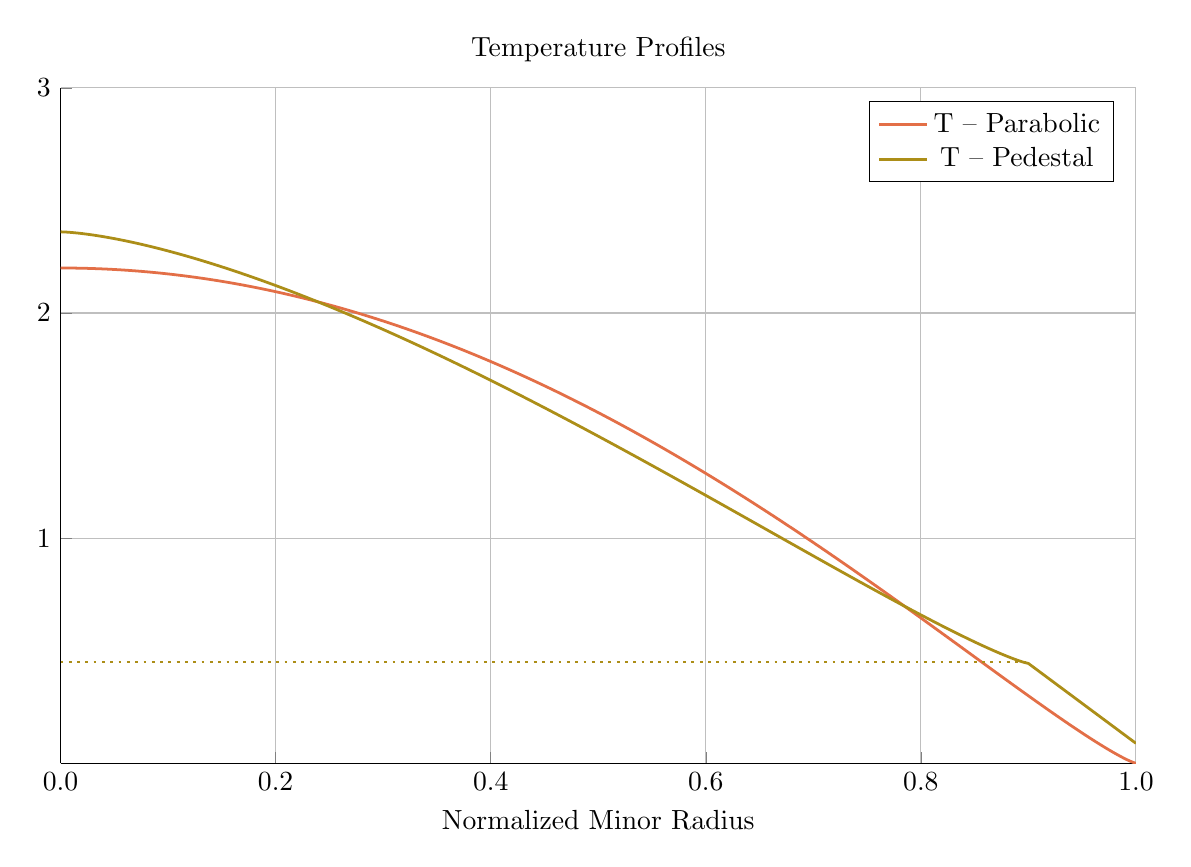
\begin{tikzpicture}[]
\begin{axis}[height = {101.6mm}, ylabel = {}, title = {Temperature Profiles}, xmin = {0.0}, xmax = {1.0}, ymax = {3}, xlabel = {Normalized Minor Radius}, {unbounded coords=jump, scaled x ticks = false, xticklabel style={rotate = 0}, xmajorgrids = true, xtick = {0.0,0.2,0.4,0.6000000000000001,0.8,1.0}, xticklabels = {0.0,0.2,0.4,0.6,0.8,1.0}, xtick align = inside, axis lines* = left, scaled y ticks = false, yticklabel style={rotate = 0}, ymajorgrids = true, ytick = {1.0,2.0,3.0}, yticklabels = {1,2,3}, ytick align = inside, axis lines* = left,     xshift = 0.0mm,
    yshift = 0.0mm,
    axis background/.style={fill={rgb,1:red,1.00000000;green,1.00000000;blue,1.00000000}}
}, ymin = {0}, width = {152.4mm}]\addplot+ [color = {rgb,1:red,0.88887350;green,0.43564919;blue,0.27812294},
draw opacity=1.0,
line width=1,
solid,mark = none,
mark size = 2.0,
mark options = {
    color = {rgb,1:red,0.00000000;green,0.00000000;blue,0.00000000}, draw opacity = 1.0,
    fill = {rgb,1:red,0.88887350;green,0.43564919;blue,0.27812294}, fill opacity = 1.0,
    line width = 1,
    rotate = 0,
    solid
}]coordinates {
(0.0, 2.2)
(0.004, 2.1999577600675844)
(0.008, 2.199831041081363)
(0.012, 2.199619845474514)
(0.016, 2.1993241773026853)
(0.02, 2.198944042244507)
(0.024, 2.1984794476023213)
(0.028, 2.1979304023031214)
(0.032, 2.1972969168996905)
(0.036, 2.196579003571959)
(0.04, 2.195776676128566)
(0.044, 2.194889950008634)
(0.048, 2.1939188422837517)
(0.052, 2.192863371660171)
(0.056, 2.1917235584812182)
(0.06, 2.1904994247299143)
(0.064, 2.189190994031813)
(0.068, 2.187798291658056)
(0.072, 2.1863213445286407)
(0.076, 2.1847601812159145)
(0.08, 2.1831148319482794)
(0.084, 2.1813853286141245)
(0.088, 2.179571704765981)
(0.092, 2.1776739956248985)
(0.096, 2.1756922380850554)
(0.1, 2.1736264707185855)
(0.104, 2.1714767337806498)
(0.108, 2.1692430692147298)
(0.112, 2.1669255206581606)
(0.116, 2.164524133447901)
(0.12, 2.1620389546265417)
(0.124, 2.1594700329485588)
(0.128, 2.1568174188868077)
(0.132, 2.154081164639269)
(0.136, 2.1512613241360428)
(0.14, 2.148357953046596)
(0.144, 2.1453711087872693)
(0.148, 2.1423008505290397)
(0.152, 2.139147239205551)
(0.156, 2.1359103375214086)
(0.16, 2.1325902099607443)
(0.164, 2.129186922796058)
(0.168, 2.1257005440973358)
(0.172, 2.1221311437414503)
(0.176, 2.1184787934218474)
(0.18, 2.1147435666585284)
(0.184, 2.1109255388083183)
(0.188, 2.1070247870754453)
(0.192, 2.1030413905224172)
(0.196, 2.098975430081212)
(0.2, 2.09482698856478)
(0.204, 2.090596150678874)
(0.208, 2.086283003034196)
(0.212, 2.0818876341588837)
(0.216, 2.0774101345113314)
(0.22, 2.072850596493357)
(0.224, 2.068209114463716)
(0.228, 2.063485784751976)
(0.232, 2.058680705672756)
(0.236, 2.053793977540332)
(0.24, 2.0488257026836245)
(0.244, 2.043775985461571)
(0.248, 2.038644932278893)
(0.252, 2.033432651602259)
(0.256, 2.0281392539768675)
(0.26, 2.022764852043437)
(0.264, 2.0173095605556335)
(0.268, 2.0117734963979244)
(0.272, 2.006156778603888)
(0.276, 2.0004595283749724)
(0.28, 1.9946818690997206)
(0.284, 1.9888239263734737)
(0.288, 1.9828858280185606)
(0.292, 1.976867704104986)
(0.296, 1.9707696869716258)
(0.3, 1.9645919112479475)
(0.304, 1.9583345138762616)
(0.308, 1.9519976341345224)
(0.312, 1.9455814136596863)
(0.316, 1.939085996471644)
(0.32, 1.932511528997742)
(0.324, 1.9258581600979061)
(0.328, 1.9191260410903783)
(0.332, 1.912315325778094)
(0.336, 1.9054261704757012)
(0.34, 1.8984587340372499)
(0.344, 1.8914131778845642)
(0.348, 1.8842896660363146)
(0.352, 1.8770883651378103)
(0.356, 1.8698094444915332)
(0.36, 1.8624530760884261)
(0.364, 1.8550194346399664)
(0.368, 1.8475086976110369)
(0.372, 1.839921045253621)
(0.376, 1.8322566606413475)
(0.38, 1.8245157297049002)
(0.384, 1.8166984412683274)
(0.388, 1.8088049870862715)
(0.392, 1.8008355618821434)
(0.396, 1.792790363387276)
(0.4, 1.7846695923810785)
(0.404, 1.776473452732227)
(0.408, 1.7682021514409176)
(0.412, 1.7598558986822177)
(0.416, 1.7514349078505493)
(0.42, 1.742939395605332)
(0.424, 1.7343695819178346)
(0.428, 1.725725690119258)
(0.432, 1.7170079469501018)
(0.436, 1.7082165826108464)
(0.44, 1.6993518308139948)
(0.444, 1.6904139288375197)
(0.448, 1.6814031175797635)
(0.452, 1.6723196416158315)
(0.456, 1.6631637492555364)
(0.46, 1.653935692602939)
(0.464, 1.6446357276175452)
(0.468, 1.6352641141772097)
(0.472, 1.6258211161428078)
(0.476, 1.6163070014247378)
(0.48, 1.606722042051314)
(0.484, 1.5970665142391203)
(0.488, 1.5873406984653924)
(0.492, 1.5775448795424998)
(0.496, 1.5676793466946068)
(0.5, 1.5577443936365882)
(0.504, 1.5477403186552856)
(0.508, 1.5376674246931867)
(0.512, 1.5275260194346267)
(0.516, 1.517316415394591)
(0.52, 1.5070389300102414)
(0.524, 1.4966938857352434)
(0.528, 1.4862816101370295)
(0.532, 1.4758024359970894)
(0.536, 1.465256701414425)
(0.54, 1.4546447499122863)
(0.544, 1.4439669305483216)
(0.548, 1.4332235980282817)
(0.552, 1.4224151128234246)
(0.556, 1.4115418412917677)
(0.56, 1.4006041558033582)
(0.564, 1.3896024348697198)
(0.568, 1.3785370632776597)
(0.572, 1.3674084322276236)
(0.576, 1.3562169394767907)
(0.58, 1.3449629894871216)
(0.584, 1.333646993578575)
(0.588, 1.3222693700877242)
(0.592, 1.3108305445320172)
(0.596, 1.2993309497799401)
(0.6, 1.2877710262273512)
(0.604, 1.2761512219802742)
(0.608, 1.2644719930444575)
(0.612, 1.2527338035220144)
(0.616, 1.2409371258154922)
(0.62, 1.2290824408397232)
(0.624, 1.2171702382418437)
(0.628, 1.2052010166298843)
(0.632, 1.1931752838103635)
(0.636, 1.1810935570353371)
(0.64, 1.1689563632593918)
(0.644, 1.156764239407098)
(0.648, 1.1445177326514693)
(0.652, 1.1322174007040144)
(0.656, 1.1198638121170017)
(0.66, 1.1074575465986056)
(0.664, 1.0949991953416336)
(0.668, 1.082489361366603)
(0.672, 1.0699286598799627)
(0.676, 1.0573177186483342)
(0.68, 1.044657178389695)
(0.684, 1.0319476931824922)
(0.688, 1.019189930893753)
(0.692, 1.0063845736273342)
(0.696, 0.9935323181935332)
(0.7, 0.980633876601379)
(0.704, 0.9676899765750238)
(0.708, 0.9547013620957563)
(0.712, 0.9416687939712927)
(0.716, 0.9285930504341149)
(0.72, 0.9154749277707805)
(0.724, 0.9023152409842818)
(0.728, 0.8891148244917015)
(0.732, 0.8758745328596077)
(0.736, 0.8625952415798288)
(0.74, 0.849277847888491)
(0.744, 0.8359232716314423)
(0.748, 0.822532456179475)
(0.752, 0.8091063693970627)
(0.756, 0.7956460046686752)
(0.76, 0.7821523819871128)
(0.764, 0.7686265491087244)
(0.768, 0.7550695827808527)
(0.772, 0.7414825900473649)
(0.776, 0.7278667096387308)
(0.78, 0.7142231134537544)
(0.784, 0.7005530081408239)
(0.788, 0.6868576367873601)
(0.792, 0.6731382807270975)
(0.796, 0.6593962614758839)
(0.8, 0.6456329428078906)
(0.804, 0.6318497329854856)
(0.808, 0.6180480871575735)
(0.812, 0.6042295099429783)
(0.816, 0.5903955582174578)
(0.82, 0.5765478441252689)
(0.824, 0.5626880383388612)
(0.828, 0.5488178735933505)
(0.832, 0.5349391485259877)
(0.836, 0.5210537318549578)
(0.84, 0.5071635669366619)
(0.844, 0.49327067674623953)
(0.848, 0.47937716933269775)
(0.852, 0.46548524380775297)
(0.856, 0.45159719693668826)
(0.86, 0.4377154304104124)
(0.864, 0.42384245889091393)
(0.868, 0.40998091893787963)
(0.872, 0.3961335789430169)
(0.876, 0.38230335022134865)
(0.88, 0.36849329943642983)
(0.884, 0.35470666257034567)
(0.888, 0.340946860691165)
(0.892, 0.3272175178224195)
(0.896, 0.31352248128407095)
(0.9, 0.2998658449561726)
(0.904, 0.28625197602028446)
(0.908, 0.2726855458667975)
(0.912, 0.25917156602852953)
(0.916, 0.24571543022609155)
(0.92, 0.23232296390814428)
(0.924, 0.21900048306792003)
(0.928, 0.20575486465742054)
(0.932, 0.1925936316637043)
(0.936, 0.17952505695042487)
(0.94, 0.16655829144594192)
(0.944, 0.15370352440467291)
(0.948, 0.14097218665156444)
(0.952, 0.12837721256189286)
(0.956, 0.11593338410667639)
(0.96, 0.10365779254585625)
(0.964, 0.09157047392306764)
(0.968, 0.07969531062880889)
(0.972, 0.06806135815914495)
(0.976, 0.056704888286093984)
(0.98, 0.04567272289384328)
(0.984, 0.035028106493367024)
(0.988, 0.024862215823612335)
(0.992, 0.0153206738078139)
(0.996, 0.0066847830139362754)
(1.0, 0.0)
};
\addlegendentry{T -- Parabolic}
\addplot+ [color = {rgb,1:red,0.67554396;green,0.55566233;blue,0.09423434},
draw opacity=1.0,
line width=1,
solid,mark = none,
mark size = 2.0,
mark options = {
    color = {rgb,1:red,0.00000000;green,0.00000000;blue,0.00000000}, draw opacity = 1.0,
    fill = {rgb,1:red,0.67554396;green,0.55566233;blue,0.09423434}, fill opacity = 1.0,
    line width = 1,
    rotate = 0,
    solid
}]coordinates {
(0.0, 2.3605919704710323)
(0.004, 2.359910398918797)
(0.008, 2.3586642994783618)
(0.012, 2.3570508613498493)
(0.016, 2.3551405297956594)
(0.02, 2.3529740696983454)
(0.024, 2.350579025743975)
(0.028, 2.3479756517769723)
(0.032, 2.3451796682823796)
(0.036, 2.342203747147281)
(0.04, 2.3390583928390996)
(0.044, 2.3357525032801973)
(0.048, 2.332293746279636)
(0.052, 2.328688822918463)
(0.056, 2.3249436581415552)
(0.06, 2.3210635425572748)
(0.064, 2.3170532404255844)
(0.068, 2.3129170735482543)
(0.072, 2.3086589875663335)
(0.076, 2.3042826051438894)
(0.08, 2.299791269197131)
(0.084, 2.295188078444673)
(0.088, 2.2904759169492626)
(0.092, 2.2856574788975115)
(0.096, 2.2807352895619175)
(0.1, 2.2757117231701707)
(0.104, 2.2705890182452353)
(0.108, 2.2653692908590712)
(0.112, 2.260054546151598)
(0.116, 2.2546466883966962)
(0.12, 2.2491475298430212)
(0.124, 2.243558798515241)
(0.128, 2.237882145128044)
(0.132, 2.2321191492388524)
(0.136, 2.2262713247439767)
(0.14, 2.220340124805883)
(0.144, 2.2143269462853388)
(0.148, 2.2082331337408316)
(0.152, 2.202059983048349)
(0.156, 2.1958087446868073)
(0.16, 2.189480626728042)
(0.164, 2.1830767975648464)
(0.168, 2.176598388406032)
(0.172, 2.1700464955636813)
(0.176, 2.163422182554496)
(0.18, 2.1567264820344176)
(0.184, 2.149960397583317)
(0.188, 2.14312490535454)
(0.192, 2.1362209556023704)
(0.196, 2.1292494740989305)
(0.2, 2.1222113634507807)
(0.204, 2.1151075043243255)
(0.208, 2.1079387565881396)
(0.212, 2.1007059603794906)
(0.216, 2.0934099371015487)
(0.22, 2.0860514903571366)
(0.224, 2.0786314068242686)
(0.228, 2.0711504570782133)
(0.232, 2.063609396364366)
(0.236, 2.0560089653257996)
(0.24, 2.0483498906890096)
(0.244, 2.040632885911039)
(0.248, 2.0328586517908898)
(0.252, 2.0250278770478602)
(0.256, 2.0171412388692334)
(0.26, 2.009199403429513)
(0.264, 2.00120302638324)
(0.268, 1.9931527533332325)
(0.272, 1.9850492202759686)
(0.276, 1.97689305402566)
(0.28, 1.9686848726184767)
(0.284, 1.9604252856982425)
(0.288, 1.9521148948848384)
(0.292, 1.9437542941264454)
(0.296, 1.9353440700366855)
(0.3, 1.9268848022176337)
(0.304, 1.9183770635696087)
(0.308, 1.9098214205885893)
(0.312, 1.9012184336520364)
(0.316, 1.8925686572938556)
(0.32, 1.883872640469185)
(0.324, 1.8751309268096423)
(0.328, 1.8663440548696335)
(0.332, 1.8575125583642822)
(0.336, 1.8486369663995004)
(0.34, 1.839717803694704)
(0.344, 1.8307555907986295)
(0.348, 1.8217508442986934)
(0.352, 1.812704077024307)
(0.356, 1.8036157982445404)
(0.36, 1.7944865138605)
(0.364, 1.7853167265927747)
(0.368, 1.776106936164285)
(0.372, 1.7668576394788444)
(0.376, 1.7575693307957496)
(0.38, 1.74824250190067)
(0.384, 1.7388776422731294)
(0.388, 1.7294752392508332)
(0.392, 1.7200357781911024)
(0.396, 1.7105597426296557)
(0.4, 1.7010476144369753)
(0.404, 1.6914998739724885)
(0.408, 1.6819170002367874)
(0.412, 1.6722994710220926)
(0.416, 1.6626477630611856)
(0.42, 1.6529623521750014)
(0.424, 1.6432437134190898)
(0.428, 1.633492321229143)
(0.432, 1.6237086495657764)
(0.436, 1.6138931720587668)
(0.44, 1.6040463621509233)
(0.444, 1.5941686932417938)
(0.448, 1.584260638831387)
(0.452, 1.5743226726641009)
(0.456, 1.5643552688730447)
(0.46, 1.5543589021249482)
(0.464, 1.544334047765842)
(0.468, 1.5342811819677138)
(0.472, 1.5242007818763206)
(0.476, 1.5140933257603746)
(0.48, 1.5039592931622903)
(0.484, 1.4937991650507099)
(0.488, 1.4836134239750187)
(0.492, 1.473402554222062)
(0.496, 1.4631670419753044)
(0.5, 1.4529073754766455)
(0.504, 1.4426240451911474)
(0.508, 1.4323175439749165)
(0.512, 1.4219883672464035)
(0.516, 1.4116370131613858)
(0.52, 1.4012639827919213)
(0.524, 1.3908697803095635)
(0.528, 1.3804549131731465)
(0.532, 1.3700198923214701)
(0.536, 1.359565232371216)
(0.54, 1.349091451820459)
(0.544, 1.3385990732581485)
(0.548, 1.328088623579961)
(0.552, 1.3175606342109392)
(0.556, 1.307015641335371)
(0.56, 1.2964541861343752)
(0.564, 1.2858768150316933)
(0.568, 1.2752840799482301)
(0.572, 1.2646765385659007)
(0.576, 1.2540547546013914)
(0.58, 1.2434192980904786)
(0.584, 1.2327707456835955)
(0.588, 1.222109680953382)
(0.592, 1.211436694715004)
(0.596, 1.200752385360086)
(0.6, 1.1900573592051713)
(0.604, 1.1793522308556705)
(0.608, 1.1686376235863563)
(0.612, 1.1579141697395272)
(0.616, 1.1471825111420575)
(0.62, 1.1364432995426441)
(0.624, 1.1256971970706737)
(0.628, 1.1149448767182386)
(0.632, 1.1041870228469695)
(0.636, 1.093424331721486)
(0.64, 1.0826575120714315)
(0.644, 1.0718872856842108)
(0.648, 1.061114388030769)
(0.652, 1.0503395689269308)
(0.656, 1.039563593233075)
(0.66, 1.0287872415951647)
(0.664, 1.0180113112304485)
(0.668, 1.0072366167614726)
(0.672, 0.9964639911023957)
(0.676, 0.9856942864020085)
(0.68, 0.9749283750483018)
(0.684, 0.9641671507399459)
(0.688, 0.9534115296306018)
(0.692, 0.9426624515526333)
(0.696, 0.9319208813275146)
(0.7, 0.9211878101710503)
(0.704, 0.9104642572024598)
(0.708, 0.8997512710674346)
(0.712, 0.8890499316865009)
(0.716, 0.8783613521413978)
(0.72, 0.8676866807137728)
(0.724, 0.8570271030923351)
(0.728, 0.8463838447667099)
(0.732, 0.8357581736286817)
(0.736, 0.8251514028043623)
(0.74, 0.8145648937441141)
(0.744, 0.8040000596009286)
(0.748, 0.7934583689324995)
(0.752, 0.7829413497675711)
(0.756, 0.7724505940834616)
(0.76, 0.7619877627491815)
(0.764, 0.7515545909975108)
(0.768, 0.741152894500166)
(0.772, 0.7307845761331225)
(0.776, 0.7204516335348546)
(0.78, 0.710156167579369)
(0.784, 0.6999003919093338)
(0.788, 0.6896866437035094)
(0.792, 0.6795173958885602)
(0.796, 0.6693952710502226)
(0.8, 0.6593230573553601)
(0.804, 0.6493037268683398)
(0.808, 0.6393404567373293)
(0.812, 0.6294366538454373)
(0.816, 0.6195959836776518)
(0.82, 0.6098224043609094)
(0.824, 0.6001202071108945)
(0.828, 0.5904940646939226)
(0.832, 0.58094909002811)
(0.836, 0.5714909077694643)
(0.84, 0.562125742755608)
(0.844, 0.5528605306710853)
(0.848, 0.5437030585117963)
(0.852, 0.5346621457948362)
(0.856, 0.5257478827341294)
(0.86, 0.516971950132737)
(0.864, 0.5083480600719166)
(0.868, 0.49989258164201933)
(0.872, 0.4916254625709785)
(0.876, 0.48357164972903754)
(0.88, 0.47576340897240366)
(0.884, 0.4682444150948954)
(0.888, 0.4610777748740693)
(0.892, 0.45436452608473005)
(0.896, 0.44830036952087016)
(0.9, 0.44361517600666117)
(0.904, 0.429419490374448)
(0.908, 0.41522380474223486)
(0.912, 0.4010281191100217)
(0.916, 0.38683243347780855)
(0.92, 0.3726367478455953)
(0.924, 0.3584410622133822)
(0.928, 0.34424537658116894)
(0.932, 0.3300496909489558)
(0.936, 0.3158540053167426)
(0.94, 0.30165831968452983)
(0.944, 0.28746263405231665)
(0.948, 0.27326694842010346)
(0.952, 0.2590712627878903)
(0.956, 0.24487557715567715)
(0.96, 0.23067989152346396)
(0.964, 0.21648420589125078)
(0.968, 0.2022885202590376)
(0.972, 0.18809283462682444)
(0.976, 0.17389714899461126)
(0.98, 0.1597014633623981)
(0.984, 0.14550577773018494)
(0.988, 0.13131009209797176)
(0.992, 0.11711440646575859)
(0.996, 0.1029187208335454)
(1.0, 0.08872303520133223)
};
\addlegendentry{T -- Pedestal}
\addplot+ [color = {rgb,1:red,0.67554396;green,0.55566233;blue,0.09423434},
draw opacity=1.0,
line width=1,
dotted,mark = none,
mark size = 2.0,
mark options = {
    color = {rgb,1:red,0.00000000;green,0.00000000;blue,0.00000000}, draw opacity = 1.0,
    fill = {rgb,1:red,0.67554396;green,0.55566233;blue,0.09423434}, fill opacity = 1.0,
    line width = 1,
    rotate = 0,
    solid
},forget plot]coordinates {
(0.0, 0.45)
(0.9, 0.45)
};
\end{axis}

\end{tikzpicture}

		\end{adjustbox}
        \caption{Temperature Profiles}
    \end{subfigure}
    \hfill \hfill ~\\ ~\\ ~\\
    \caption{Radial Plasma Profiles} ~\\
    \small The three most fundamental properties of a fusion plasma are its temperature, density, and current. These profiles allow the model to reduce from three dimensions to half of one.
\end{figure*}

\section{Density -- $n$}

The Density is important to us. We use it in the Greenwald density limit, so it should be clean in both line-averaged and volume-averaged forms. Because of its flat profile, a parabola is a good approximation for H-mode pulses:

\begin{equation}
	n(\rho) = \overline{n} \cdot \left(1 + \nu_n \right) \cdot \left( 1 - \rho^2  \right)^{\nu_n}
\end{equation}

The line average density is related to $\overline{n}$ through:

\begin{equation}
	\hat{n} =  \overline{n} \cdot \left( \frac{\pi ^ { \, 1/2} }{2} \right)  \cdot \, \frac{ \Gamma( \, \nu_n + 2 \, ) }{ \Gamma( \, \nu_n + 3/2 \, ) }
\end{equation}

The convenience of this function comes from how the volumetric average comes out.

To relate this to the volume integral, we use:

\begin{equation}
	\overline{x} = \frac{1}{\volume} \int x(\rho) \, d\volume
\end{equation}

For a normalized radial profile that does not depend on angle,

\begin{equation}
	\volume = \int_0^1 \rho \, d\rho = \sfrac{1}{2}
\end{equation}

Then, when $x = n$,

\begin{equation}
	\overline{n} = 2 \int_0^1 n(\rho) \rho \, d\rho = \overline{n}
\end{equation}

Additionally, the Greenwald Density limit that we will use throughout,
\begin{equation}
	\hat{n} = N_G \cdot \left( \frac{I_M}{\pi a^2} \right) 
\end{equation} 

can now be written in the following form:
\begin{equation}
	\overline{n} =K_{n} \cdot \left( \frac{I_M}{R_0^{\,2}} \right)
\end{equation} 
\begin{equation}
	K_n = \frac{2 \, N_G}{\epsilon^2 \pi ^ { \, 3/2} }\cdot \left( \frac{ \Gamma( \, \nu_n + 3/2 \, ) }{ \Gamma( \, \nu_n + 2 \, ) } \right)
\end{equation}

\section{Temperature -- $T$}

The Temperature is the swept variable in our model framework. Therefore, it's the one we can allow people to be the most cavalier with. Additionally, as temperature profiles are highly peaked, their pedestal region is sometimes wrongfully neglected with a parabola.

\begin{equation}
	T(\rho) = \overline{T} \cdot \left(1 + \nu_T \right) \cdot \left( 1 - \rho^2  \right)^{\nu_T}
\end{equation}

Therefore, our model sometimes treats the system as if it had a pedestal region. This is mainly for the bootstrap current and fusion power, which were previously known to misalign and overshoot, respectively.
\begin{equation}
	\tcboxmath{
	T(\rho) = 
	\begin{cases}
	    T_{para} \ , & x \in [0, \rho_{ped} ] \\
	    T_{line}   \ , & x \in ( \rho_{ped}, 1 ]
	\end{cases}
	}	
\end{equation}

Where the piecewise functions are given by,
\begin{equation}
	T_{para} = T_{ped} + ( T_{0} - T_{ped} ) \cdot \left( 1 - \left( \frac{\rho}{\rho_{ped}} \right)^{\lambda_T} \right)^{\nu_T}
\end{equation}
\begin{equation}
	T_{line} = T_{sep} + ( T_{ped} - T_{sep} ) \cdot \left( \frac{ 1 - \rho }{ 1 - \rho_{ped} } \right)
\end{equation}

This temperature profile is related to the volume-averaged temperature through,

\begin{equation}
	\overline{T} \cdot \volume = \int_0^{\rho_{ped}} T_{para}(\rho) \, \rho \, d\rho + \int_{\rho_{ped}}^1 T_{line}(\rho) \, \rho \, d\rho
\end{equation}

Starting with the second integral,

\begin{equation}
	\int_{\rho_{ped}}^1 T_{line}(\rho) \, \rho \, d\rho = \frac{1}{3} \cdot ( 1 - \rho_{ped} ) \cdot \left( \left( T_{sep} + \sfrac{ T_{ped} }{2} \right) + \rho_{ped} \cdot \left( T_{ped} + \sfrac{ T_{sep} }{2}  \right)  \right)
\end{equation}

The first integral can be handled by breaking it into to,
\begin{multline}
	\int_0^{\rho_{ped}} T_{para}(\rho) \, \rho \, d\rho = T_{ped} \cdot \int_0^{\rho_{ped}} \rho \, d\rho \ + \\ ( T_{0} - T_{ped} ) \cdot \int_0^{\rho_{ped}} \left( 1 - \left( \frac{\rho}{\rho_{ped}} \right)^{\lambda_T} \right)^{\nu_T}  \cdot \rho \, d\rho \ \ \  \
\end{multline}

The first sub-integral is then,
\begin{equation}
	T_{ped} \cdot \int_0^{\rho_{ped}} \rho \, d\rho = \frac{ T_{ped} \, \rho_{ped}^{\,2} }{2}
\end{equation}

Utilizing the following transformation,
\begin{equation}
	u = \frac{\rho}{\rho_{ped}}
\end{equation}
\begin{equation}
	d\rho = \rho_{ped} \, du
\end{equation}
\begin{equation}
	u( \rho=\rho_{ped} ) = 1
\end{equation}

The second sub-integral becomes (assuming independence from $T_0$ and $T_{ped}$),
\begin{equation}
	( T_{0} - T_{ped} ) \cdot \rho_{ped}^2 \cdot \int_0^{1} \left( 1 - u^{\,\lambda_T} \right)^{\nu_T}  \cdot u \, du
\end{equation}

Where:
\begin{equation}
	\int_0^{1} \left( 1 - u^{\,\lambda_T} \right)^{\nu_T}  \cdot u \, du =  \frac{ \Gamma \left( 1 + \nu_T  \right) \Gamma \left( \frac{2}{\lambda_T} \right) }{ \lambda_T \cdot \Gamma \left( 1 + \nu_T + \frac{2}{\lambda_T} \right) }
\end{equation}

We are now in a position to solve for $T_0$ in terms of $\overline{T}$:
\begin{equation}
	\tcboxmath{
	T_0 = T_{ped} + \frac{ \overline{T} - K_{TU} }{K_{TD}} }
\end{equation}
\begin{equation}
	K_{TU}  =  T_{ped} \, \rho_{ped}^{\,2}  \ +  \frac{ \left( 1 - \rho_{ped} \right ) }{3} \cdot \left( \left( 2 T_{sep} + T_{ped} \right) + \rho_{ped} \cdot \left( 2 T_{ped} + T_{sep}   \right)  \right) 
\end{equation}
\begin{equation}
	K_{TD} = \rho_{ped}^2 \cdot \left( \frac{ 2 }{ \lambda_T } \right) \, \cdot \frac{ \Gamma \left( 1 + \nu_T  \right) \Gamma \left( \frac{2}{\lambda_T} \right) }{ \Gamma \left( 1 + \nu_T + \frac{2}{\lambda_T} \right) }
\end{equation}

Which although not pretty, can be plugged into the original equation.

\section{Pressure -- $p$}

The first point to make is that we are not using the same temperature profile for the pressure as for the temperature. This is because it would lead to hypergeometric functions that are not worth the headache.

As most of the pressure is at the center, we use simple parabolic profile. This leads to:

\begin{equation}
	\overline{p} = 0.1581 \, ( 1 + f_D ) \, \frac{ (1 + \nu_n) \, (1 + \nu_T) }{1 + \nu_n + \nu_T } \, \overline{n} \, \overline{T} \ \ [atm]
\end{equation}

\section{Bootstrap Current -- $f_{BS}$}

We start with,

\begin{equation}
	f_{BS} = \frac{I_{BS}}{I_P} = \frac{ 2 \pi a^2 \kappa }{I_P} \int_0^1 J_B \, \rho \, d\rho
\end{equation}

Expanding the previous equation using the following relations,
\begin{equation}
	J_B = -4.85 \cdot R_0 \epsilon^{1/2} \cdot \left( \frac{ \rho^{1/2} n T }{ \sfrac{ \textnormal{d}\psi }{ \textnormal{d}\rho } } \right) \cdot \left( \frac{ \sfrac{ \textnormal{d}n }{ \textnormal{d}\rho } }{ n } + 0.54 \cdot \frac{ \sfrac{ \textnormal{d}T }{ \textnormal{d}\rho } }{ T } \right)
\end{equation}
\begin{equation}
	\frac{ \textnormal{d}\psi }{ \textnormal{d}\rho } = \frac{ \mu_0 R_0 I_P }{ \pi } \cdot \left( \frac{ \kappa}{1+\kappa^2} \right) \cdot b_p(\rho)
\end{equation}

Yields:
\begin{equation}
	f_{BS} = -K_{BS} \int_0^1 \left( 1 - \rho^2  \right)^{\nu_n} \cdot \left( \frac{ \rho^{3/2} }{ b_p(\rho) } \right) \cdot \left( \frac{T}{ n } \cdot  \frac{ \textnormal{d}n }{ \textnormal{d}\rho } + 0.54 \cdot  \frac{ \textnormal{d}T }{ \textnormal{d}\rho }  \right)
 \, d\rho
\end{equation}
\begin{equation}
	K_{BS} = K_n \cdot \left( \frac{ 2 \pi^2 \cdot 4.85 \cdot \epsilon^{5/2} }{\mu_0} \right) \cdot ( 1 + \nu_n ) \cdot ( 1 + \kappa^2 )
\end{equation}

Here, $b_p$ comes from:
\begin{equation}
	b_p(\rho) = \frac{ -e^{\gamma\rho^2} ( \gamma\rho^2 - 1 - \gamma ) - 1 - \gamma }{\rho \,( e^\gamma - 1 - \gamma ) }
\end{equation}

And the value of $\gamma$ comes from the the normalized internal inductance:

\begin{equation}
	l_i = \frac{4 \kappa}{1+\kappa^2}	 \int_0^1 b_p^2 \ \frac{d\rho}{\rho}
\end{equation}

With our profiles,
\begin{equation}
	-\left( \frac{T}{n} \cdot \frac{ \textnormal{d}n }{ \textnormal{d}\rho } \right) = 2 \nu_n \cdot \left( \frac{ T \cdot \rho }{ 1 - \rho^2 } \right)
\end{equation}

While treating temperature differently results in,
\begin{equation}
	-\left( \frac{ \textnormal{d}T }{ \textnormal{d}\rho } \right)_{para} =  \left( \frac{ T_0 - T_{ped} }{ \rho_{ped}^{ \, \lambda_T} } \right) \cdot ( \nu_T \lambda_T ) \cdot \rho^{\,\lambda_T-1} \cdot \left( 1 - \left( \frac{\rho}{\rho_{ped}} \right)^{\lambda_T} \right)^{\nu_T-1}
\end{equation}
\begin{equation}
	-\left( \frac{ \textnormal{d}T }{ \textnormal{d}\rho } \right)_{line} =  \left( \frac{ T_{ped} - T_{sep} }{1 - \rho_{ped} } \right) 
\end{equation}

Where we will be using the new symbol definition,
\begin{equation}
	\partial{T} = -\left( \frac{ \textnormal{d}T }{ \textnormal{d}\rho } \right)
\end{equation}

Which ultimately allows us to write,
\begin{empheq}[box=\tcbhighmath]{gather}
	f_{BS} = K_{BS} \int_0^1 H_{BS} \, d\rho \\
	H_{BS} = \left( 1 - \rho^2  \right)^{\nu_n-1} \cdot \left( \frac{ \rho^{3/2} }{ b_p(\rho) } \right) \cdot \bigg( 2 \nu_n \cdot \rho \cdot T + 0.54 \cdot \left( 1 - \rho^2 \right) \cdot \partial{T}   \bigg)
\end{empheq}

Where the values of $T$ are determined through,
\begin{equation}
	T_{para} = T_{ped} + ( T_{0} - T_{ped} ) \cdot \left( 1 - \left( \frac{\rho}{\rho_{ped}} \right)^{\lambda_T} \right)^{\nu_T}
\end{equation}
\begin{equation}
	T_{line} = T_{sep} + ( T_{ped} - T_{sep} ) \cdot \left( \frac{ 1 - \rho }{ 1 - \rho_{ped} } \right)
\end{equation}

And the values of $\partial{T}$ are:
\begin{equation}
	\partial{T}_{para} =  \left( \frac{ T_0 - T_{ped} }{ \rho_{ped}^{ \, \lambda_T} } \right) \cdot ( \nu_T \lambda_T ) \cdot \rho^{\,\lambda_T-1} \cdot \left( 1 - \left( \frac{\rho}{\rho_{ped}} \right)^{\lambda_T} \right)^{\nu_T-1}
\end{equation}
\begin{equation}
	\partial{T}_{line} =  \left( \frac{ T_{ped} - T_{sep} }{1 - \rho_{ped} } \right) 
\end{equation}

\section{Reactivity -- $(\sigma v)$}

When discussing reactivity, the place to start is talking about fusion power,
\begin{equation}
	P_F = \int E_F \, n_D \, n_T \, \langle \sigma v \rangle \, d \textbf{r}
\end{equation}

For the tokamak geometry given, volume integrals can be reduced to 0-D forms. 

An arbitrary $F(\rho)$ has that:
\begin{equation}
	F_V = 4 \, \pi ^2 \, R_0 \, a^2 \kappa \, g \int\limits_0^1 F(\rho) \rho d\rho
\end{equation}

Given that $E_F = 17.6$ MeV and,
\begin{equation}
	n_D = n_T = f_D \frac {n_e}{2} = \frac{f_D}{2} \cdot \, \left( \ \overline{n} \, ( 1 + \nu_n ) \, ( 1 - \rho^2 ) ^ {\, \nu_n} \, \right) 
\end{equation}

Fusion power can be expressed as,
\begin{equation}
	P_F = K_F \cdot ( \, \overline{n}^2 \, R_0^3 \, ) \cdot (\sigma v) \ \ \ [MW]
\end{equation}
\begin{equation}
	 (\sigma v) = 10^{21} \, (1+\nu_n)^2 \int\limits_0^1 ( 1 - \rho^2 ) ^ { \, 2 \nu_n} \langle \sigma v \rangle \, \rho \, d\rho
\end{equation}
\begin{equation}
	K_F = 278.3 \, ( f_D^2 \, \epsilon^2 \kappa \, g )
\end{equation}

The Bosch-Hale parametrization of the volumetric reaction rates is then given by,
\begin{equation}
	\tcboxmath{
	\langle \sigma v \rangle = C_1 \cdot \theta \cdot \textnormal{exp}(-3 \xi) \cdot \sqrt{ \frac{\xi  }{m_\mu  c^2 T^3} }  \ \ \, [ \, \sfrac{ \textnormal{m}^3 }{ \textnormal{s} } \, ] }
\end{equation}
\begin{equation} 
	\theta = T \cdot \left(1-\frac{T(C_2+T(C_4+TC_6))}{1+T(C_3+T(C_5+TC_7))}\right) ^{-1}
\end{equation}
\begin{equation}
	\xi = \left(\frac{B_G^2}{4\theta}\right)^{1/3}
\end{equation}

Where approximate DT volumetric reaction rate ($10\lesssim~T~\mathrm{[keV]}\lesssim20$)
\begin{equation}
		\langle\sigma v\rangle_\mathrm{DT} = 1.1\times10^{-24} \cdot  \, T^2   \ \ \ [ \, \sfrac{ \textnormal{m}^3 }{ \textnormal{s} } \, ]
\end{equation}

In our model, each appearance of T is set to the pedestal profile defined earlier.

\begin{table}[h!]\small
  \noindent
  \centering
  \begin{tabular}{c | c c | c | c}
    \multicolumn{5}{c}{Bosch-Hale parametrization coefficients for volumetric reaction rates}\\
    \hline
    & $^2$H(d,n)$^3$He & $^2$H(d,p)$^3$H & $^3H$(d,n)$^4$He & $^3$He(d,p)$^4$He\\
    \hline\hline
    B$_G$ [keV$^{1/2}$] & 31.3970 & 31.3970 & 34.3827   & 68.7508 \\
    $m_\mu c^2$ [keV]   & 937 814 & 937 814 & 1 124 656 & 1 124 572 \\
    \hline
            % 2H(d,n)                    % 2H(d,p)                   % 3H(d,n)                    % 3He(d,p)
    C$_1$& 5.43360$\times$10$^{-12}$  & 5.65718$\times$10$^{-12}$ & 1.17302$\times$10$^{-9}$  & 5.51036$\times$10$^{-10}$ \\ 
    C$_2$  & 5.85778$\times$10$^{-3}$   & 3.41267$\times$10$^{-3}$  & 1.51361$\times$10$^{-2}$  & 6.41918$\times$10$^{-3}$ \\
    C$_3$  & 7.68222$\times$10$^{-3}$   & 1.99167$\times$10$^{-3}$  & 7.51886$\times$10$^{-2}$  & -2.02896$\times$10$^{-3}$ \\
    C$_4$  & 0.0                        & 0.0                       & 4.60643$\times$10$^{-3}$  & -1.91080$\times$10$^{-5}$ \\
    C$_5$  & -2.96400$\times$10$^{-6}$  & 1.05060$\times$10$^{-5}$  & 1.35000$\times$10$^{-2}$  & 1.35776$\times$10$^{-4}$ \\
    C$_6$  & 0.0                        & 0.0                       & -1.06750$\times$10$^{-4}$ & 0.0 \\
    C$_7$& 0.0                      & 0.0                       & 1.36600$\times$10$^{-5}$  & 0.0 \\
    \hline
    Valid range (keV) & 0.2$<$T$_i<$100 & 0.2$<$T$_i<$100 & 0.2$<$T$_i<$100 & 0.5$<$T$_i<$190\\
    \hline
  \end{tabular}
  \label{table:rrParam}
\end{table}

\begin{table}[h!]\small
  \noindent
  \centering
  \begin{tabular}{c | c c | c | c}
    \multicolumn{5}{c}{Tabulated Bosch-Hale reaction rates [m$^3$~s$^{-1}$]}\\
    \hline
    T (keV) & $^2$H(d,n)$^3$He & $^2$H(d,p)$^3$H & $^3H$(d,n)$^4$He & $^3$He(d,p)$^4$He\\
    \hline\hline
    1.0& 9.933$\times$10$^{-29}$ & 1.017$\times$10$^{-28}$ & 6.857$\times$10$^{-27}$ & 3.057$\times$10$^{-32}$ \\
    1.5  & 8.284$\times$10$^{-28}$ & 8.431$\times$10$^{-28}$ & 6.923$\times$10$^{-26}$ & 1.317$\times$10$^{-30}$ \\
    2.0  & 3.110$\times$10$^{-27}$ & 3.150$\times$10$^{-27}$ & 2.977$\times$10$^{-25}$ & 1.399$\times$10$^{-29}$ \\
    3.0  & 1.602$\times$10$^{-26}$ & 1.608$\times$10$^{-26}$ & 1.867$\times$10$^{-24}$ & 2.676$\times$10$^{-28}$ \\
    4.0  & 4.447$\times$10$^{-26}$ & 4.428$\times$10$^{-26}$ & 5.974$\times$10$^{-24}$ & 1.710$\times$10$^{-27}$ \\
    5.0  & 9.128$\times$10$^{-26}$ & 9.024$\times$10$^{-26}$ & 1.366$\times$10$^{-23}$ & 6.377$\times$10$^{-27}$ \\
    8.0  & 3.457$\times$10$^{-25}$ & 3.354$\times$10$^{-25}$ & 6.222$\times$10$^{-23}$ & 7.504$\times$10$^{-26}$ \\
   10.0  & 6.023$\times$10$^{-25}$ & 5.781$\times$10$^{-25}$ & 1.136$\times$10$^{-22}$ & 2.126$\times$10$^{-25}$ \\
   12.0  & 9.175$\times$10$^{-25}$ & 8.723$\times$10$^{-25}$ & 1.747$\times$10$^{-22}$ & 4.715$\times$10$^{-25}$ \\
   15.0  & 1.481$\times$10$^{-24}$ & 1.390$\times$10$^{-24}$ & 2.740$\times$10$^{-22}$ & 1.175$\times$10$^{-24}$ \\
   20.0& 2.603$\times$10$^{-24}$ & 2.399$\times$10$^{-24}$ & 4.330$\times$10$^{-22}$ & 3.482$\times$10$^{-24}$ \\
   \hline
  \end{tabular}
  \label{table:rr}
\end{table}

\section{Volume Averaged Powers}

The first thing to consider in a fusion reactor is power balance. \\ It is what separates a profitable device from a toaster. It's given by:

\label{pwr_bal}
\begin{equation}
\tcboxmath{
P_\alpha + P_H = P_\kappa + P_B }
\end{equation}
\begin{equation}
	P_\alpha = \frac{P_F}{5}
\end{equation}
\begin{equation}
	P_H = \frac{P_F}{Q}
\end{equation}
\begin{equation}
	P_\kappa = \frac{3}{2 \, \tau_E} \int p \, d\textbf{r} \ \ \ \ [ \, 3D \, ]
\end{equation}
\begin{equation}
	P_B = 5.35e3 \, Z_{eff} \int n_{\overline{n}}^2 \, \sqrt{T} \, d\textbf{r} \ \ \ \ [ \, 3D \, ]
\end{equation}

As mentioned before, $P_F$ is handled by $(\sigma v)$ and therefore the lefthand-side uses the pedestal temperature profiles. However, for the same reasons as discussed earlier, the righthand-side ($P_\kappa$ and $P_B$) need to use the parabolic temperature profiles.

Using the parabolic profiles (for $n$ and $T$) gives for the Bremsstrahlung radiation,
\begin{equation}
	P_B = K_B \cdot \left( R_0^3 \ \overline{n}^2 \, \sqrt{\,\overline{T}} \ \right) \ \ [MW]
\end{equation}
\begin{equation}
	K_B = 0.1056 \cdot Z_{eff} \cdot ( \, \epsilon^2 \, \kappa \, g \, ) \cdot \frac{ (1+\nu_n)^2 \, (1+\nu_T)^{1/2} }{1+2 \, \nu_n + 0.5 \, \nu_T}
\end{equation}

And a similar exercise for the thermal conduction losses results in:
\begin{equation}
	P_\kappa = K_\kappa \cdot \left( \frac{ R_0 ^ 3 \ \overline{n}  \, \overline{T} }{\tau_E} \right) \ \ [MW]
\end{equation}
\begin{equation}
	K_\kappa = 0.4744 \cdot  ( 1 + f_D ) \cdot ( \, \epsilon^2 \, \kappa \, g \, ) \cdot \frac{ (1 + \nu_n) \, (1 + \nu_T) }{1 + \nu_n + \nu_T }
\end{equation}

\clearpage
\newpage







%% This defines the bibliography file (main.bib) and the bibliography style.
%% If you want to create a bibliography file by hand, change the contents of
%% this file to a `thebibliography' environment.  For more information
%% see section 4.3 of the LaTeX manual.
\addcontentsline{toc}{chapter}{References}
\begin{singlespace}
\bibliography{main}
%\bibliographystyle{plain}
\bibliographystyle{ieeetr}
\end{singlespace}


\end{document}
  